\documentclass[a4paper]{book}
\usepackage{makeidx}
\usepackage{natbib}
\usepackage{graphicx}
\usepackage{multicol}
\usepackage{float}
\usepackage{listings}
\usepackage{color}
\usepackage{ifthen}
\usepackage[table]{xcolor}
\usepackage{textcomp}
\usepackage{alltt}
\usepackage{ifpdf}
\ifpdf
\usepackage[pdftex,
            pagebackref=true,
            colorlinks=true,
            linkcolor=blue,
            unicode
           ]{hyperref}
\else
\usepackage[ps2pdf,
            pagebackref=true,
            colorlinks=true,
            linkcolor=blue,
            unicode
           ]{hyperref}
\usepackage{pspicture}
\fi
\usepackage[utf8]{inputenc}
\usepackage{mathptmx}
\usepackage[scaled=.90]{helvet}
\usepackage{courier}
\usepackage{sectsty}
\usepackage[titles]{tocloft}
\usepackage{doxygen}
\lstset{language=C++,inputencoding=utf8,basicstyle=\footnotesize,breaklines=true,breakatwhitespace=true,tabsize=8,numbers=left }
\makeindex
\setcounter{tocdepth}{3}
\renewcommand{\footrulewidth}{0.4pt}
\renewcommand{\familydefault}{\sfdefault}
\hfuzz=15pt
\setlength{\emergencystretch}{15pt}
\hbadness=750
\tolerance=750
\begin{document}
\hypersetup{pageanchor=false,citecolor=blue}
\begin{titlepage}
\vspace*{7cm}
\begin{center}
{\Large \-E\-P\-A\-X\-Developer\-Guide \\[1ex]\large 0.\-01 }\\
\vspace*{1cm}
{\large \-Generated by Doxygen 1.7.6.1}\\
\vspace*{0.5cm}
{\small Fri Feb 7 2014 09:40:40}\\
\end{center}
\end{titlepage}
\clearemptydoublepage
\pagenumbering{roman}
\tableofcontents
\clearemptydoublepage
\pagenumbering{arabic}
\hypersetup{pageanchor=true,citecolor=blue}
\chapter{\-Namespace \-Index}
\section{\-Namespace \-List}
\-Here is a list of all namespaces with brief descriptions\-:\begin{DoxyCompactList}
\item\contentsline{section}{\hyperlink{namespace_e_p_a_x}{\-E\-P\-A\-X} }{\pageref{namespace_e_p_a_x}}{}
\end{DoxyCompactList}

\chapter{\-Class \-Index}
\section{\-Class \-Hierarchy}
\-This inheritance list is sorted roughly, but not completely, alphabetically\-:\begin{DoxyCompactList}
\item \contentsline{section}{\-E\-P\-A\-X\-:\-:dyn\-\_\-bitset}{\pageref{class_e_p_a_x_1_1dyn__bitset}}{}
\item \contentsline{section}{\-E\-P\-A\-X\-Export}{\pageref{class_e_p_a_x_export}}{}
\begin{DoxyCompactList}
\item \contentsline{section}{\-E\-P\-A\-X\-:\-:\-Basic\-Block}{\pageref{class_e_p_a_x_1_1_basic_block}}{}
\item \contentsline{section}{\-E\-P\-A\-X\-:\-:\-Binary}{\pageref{class_e_p_a_x_1_1_binary}}{}
\item \contentsline{section}{\-E\-P\-A\-X\-:\-:\-Control\-Flow}{\pageref{class_e_p_a_x_1_1_control_flow}}{}
\item \contentsline{section}{\-E\-P\-A\-X\-:\-:\-Function}{\pageref{class_e_p_a_x_1_1_function}}{}
\item \contentsline{section}{\-E\-P\-A\-X\-:\-:\-Instruction}{\pageref{class_e_p_a_x_1_1_instruction}}{}
\item \contentsline{section}{\-E\-P\-A\-X\-:\-:\-Loop}{\pageref{class_e_p_a_x_1_1_loop}}{}
\item \contentsline{section}{\-E\-P\-A\-X\-:\-:\-Section}{\pageref{class_e_p_a_x_1_1_section}}{}
\begin{DoxyCompactList}
\item \contentsline{section}{\-E\-P\-A\-X\-:\-:\-String\-Table}{\pageref{class_e_p_a_x_1_1_string_table}}{}
\begin{DoxyCompactList}
\item \contentsline{section}{\-E\-P\-A\-X\-:\-:\-Elf\-:\-:\-Elf\-String\-Table}{\pageref{class_e_p_a_x_1_1_elf_1_1_elf_string_table}}{}
\end{DoxyCompactList}
\item \contentsline{section}{\-E\-P\-A\-X\-:\-:\-Symbol\-Table}{\pageref{class_e_p_a_x_1_1_symbol_table}}{}
\begin{DoxyCompactList}
\item \contentsline{section}{\-E\-P\-A\-X\-:\-:\-Elf\-:\-:\-Elf\-Symbol\-Table}{\pageref{class_e_p_a_x_1_1_elf_1_1_elf_symbol_table}}{}
\end{DoxyCompactList}
\end{DoxyCompactList}
\item \contentsline{section}{\-E\-P\-A\-X\-:\-:\-Symbol}{\pageref{class_e_p_a_x_1_1_symbol}}{}
\begin{DoxyCompactList}
\item \contentsline{section}{\-E\-P\-A\-X\-:\-:\-Elf\-:\-:\-Elf\-Symbol}{\pageref{class_e_p_a_x_1_1_elf_1_1_elf_symbol}}{}
\begin{DoxyCompactList}
\item \contentsline{section}{\-E\-P\-A\-X\-:\-:\-Elf\-:\-:\-Elf\-Symbol32}{\pageref{class_e_p_a_x_1_1_elf_1_1_elf_symbol32}}{}
\item \contentsline{section}{\-E\-P\-A\-X\-:\-:\-Elf\-:\-:\-Elf\-Symbol64}{\pageref{class_e_p_a_x_1_1_elf_1_1_elf_symbol64}}{}
\end{DoxyCompactList}
\end{DoxyCompactList}
\end{DoxyCompactList}
\item \contentsline{section}{\-E\-P\-A\-X\-:\-:\-File\-Base}{\pageref{class_e_p_a_x_1_1_file_base}}{}
\begin{DoxyCompactList}
\item \contentsline{section}{\-E\-P\-A\-X\-:\-:\-Detached\-Text}{\pageref{class_e_p_a_x_1_1_detached_text}}{}
\begin{DoxyCompactList}
\item \contentsline{section}{\-E\-P\-A\-X\-:\-:\-Function}{\pageref{class_e_p_a_x_1_1_function}}{}
\end{DoxyCompactList}
\item \contentsline{section}{\-E\-P\-A\-X\-:\-:\-Elf\-:\-:\-File\-Header}{\pageref{class_e_p_a_x_1_1_elf_1_1_file_header}}{}
\begin{DoxyCompactList}
\item \contentsline{section}{\-E\-P\-A\-X\-:\-:\-Elf\-:\-:\-File\-Header32}{\pageref{class_e_p_a_x_1_1_elf_1_1_file_header32}}{}
\item \contentsline{section}{\-E\-P\-A\-X\-:\-:\-Elf\-:\-:\-File\-Header64}{\pageref{class_e_p_a_x_1_1_elf_1_1_file_header64}}{}
\end{DoxyCompactList}
\item \contentsline{section}{\-E\-P\-A\-X\-:\-:\-Elf\-:\-:\-Program\-Header}{\pageref{class_e_p_a_x_1_1_elf_1_1_program_header}}{}
\begin{DoxyCompactList}
\item \contentsline{section}{\-E\-P\-A\-X\-:\-:\-Elf\-:\-:\-Program\-Header32}{\pageref{class_e_p_a_x_1_1_elf_1_1_program_header32}}{}
\item \contentsline{section}{\-E\-P\-A\-X\-:\-:\-Elf\-:\-:\-Program\-Header64}{\pageref{class_e_p_a_x_1_1_elf_1_1_program_header64}}{}
\end{DoxyCompactList}
\item \contentsline{section}{\-E\-P\-A\-X\-:\-:\-Elf\-:\-:\-Section\-Header}{\pageref{class_e_p_a_x_1_1_elf_1_1_section_header}}{}
\begin{DoxyCompactList}
\item \contentsline{section}{\-E\-P\-A\-X\-:\-:\-Elf\-:\-:\-Section\-Header32}{\pageref{class_e_p_a_x_1_1_elf_1_1_section_header32}}{}
\item \contentsline{section}{\-E\-P\-A\-X\-:\-:\-Elf\-:\-:\-Section\-Header64}{\pageref{class_e_p_a_x_1_1_elf_1_1_section_header64}}{}
\end{DoxyCompactList}
\item \contentsline{section}{\-E\-P\-A\-X\-:\-:\-Mach\-O\-:\-:\-Mach\-Header}{\pageref{class_e_p_a_x_1_1_mach_o_1_1_mach_header}}{}
\begin{DoxyCompactList}
\item \contentsline{section}{\-E\-P\-A\-X\-:\-:\-Mach\-O\-:\-:\-Mach\-Header32}{\pageref{class_e_p_a_x_1_1_mach_o_1_1_mach_header32}}{}
\item \contentsline{section}{\-E\-P\-A\-X\-:\-:\-Mach\-O\-:\-:\-Mach\-Header64}{\pageref{class_e_p_a_x_1_1_mach_o_1_1_mach_header64}}{}
\end{DoxyCompactList}
\item \contentsline{section}{\-E\-P\-A\-X\-:\-:\-Section}{\pageref{class_e_p_a_x_1_1_section}}{}
\item \contentsline{section}{\-E\-P\-A\-X\-:\-:\-Symbol}{\pageref{class_e_p_a_x_1_1_symbol}}{}
\end{DoxyCompactList}
\item \contentsline{section}{\-E\-P\-A\-X\-:\-:\-Index\-Base}{\pageref{class_e_p_a_x_1_1_index_base}}{}
\begin{DoxyCompactList}
\item \contentsline{section}{\-E\-P\-A\-X\-:\-:\-Basic\-Block}{\pageref{class_e_p_a_x_1_1_basic_block}}{}
\item \contentsline{section}{\-E\-P\-A\-X\-:\-:\-Detached\-Text}{\pageref{class_e_p_a_x_1_1_detached_text}}{}
\item \contentsline{section}{\-E\-P\-A\-X\-:\-:\-Elf\-:\-:\-Program\-Header}{\pageref{class_e_p_a_x_1_1_elf_1_1_program_header}}{}
\item \contentsline{section}{\-E\-P\-A\-X\-:\-:\-Elf\-:\-:\-Section\-Header}{\pageref{class_e_p_a_x_1_1_elf_1_1_section_header}}{}
\item \contentsline{section}{\-E\-P\-A\-X\-:\-:\-Instruction}{\pageref{class_e_p_a_x_1_1_instruction}}{}
\item \contentsline{section}{\-E\-P\-A\-X\-:\-:\-Loop}{\pageref{class_e_p_a_x_1_1_loop}}{}
\item \contentsline{section}{\-E\-P\-A\-X\-:\-:\-Section}{\pageref{class_e_p_a_x_1_1_section}}{}
\item \contentsline{section}{\-E\-P\-A\-X\-:\-:\-Symbol}{\pageref{class_e_p_a_x_1_1_symbol}}{}
\end{DoxyCompactList}
\item \contentsline{section}{\-E\-P\-A\-X\-:\-:\-Memory\-Base}{\pageref{class_e_p_a_x_1_1_memory_base}}{}
\begin{DoxyCompactList}
\item \contentsline{section}{\-E\-P\-A\-X\-:\-:\-Basic\-Block}{\pageref{class_e_p_a_x_1_1_basic_block}}{}
\item \contentsline{section}{\-E\-P\-A\-X\-:\-:\-Detached\-Text}{\pageref{class_e_p_a_x_1_1_detached_text}}{}
\item \contentsline{section}{\-E\-P\-A\-X\-:\-:\-Elf\-:\-:\-Program\-Header}{\pageref{class_e_p_a_x_1_1_elf_1_1_program_header}}{}
\item \contentsline{section}{\-E\-P\-A\-X\-:\-:\-Instruction}{\pageref{class_e_p_a_x_1_1_instruction}}{}
\item \contentsline{section}{\-E\-P\-A\-X\-:\-:\-Section}{\pageref{class_e_p_a_x_1_1_section}}{}
\item \contentsline{section}{\-E\-P\-A\-X\-:\-:\-Symbol}{\pageref{class_e_p_a_x_1_1_symbol}}{}
\end{DoxyCompactList}
\item \contentsline{section}{\-E\-P\-A\-X\-:\-:\-Name\-Base}{\pageref{class_e_p_a_x_1_1_name_base}}{}
\begin{DoxyCompactList}
\item \contentsline{section}{\-E\-P\-A\-X\-:\-:\-Base\-Binary}{\pageref{class_e_p_a_x_1_1_base_binary}}{}
\begin{DoxyCompactList}
\item \contentsline{section}{\-E\-P\-A\-X\-:\-:\-Elf\-:\-:\-Elf\-Binary}{\pageref{class_e_p_a_x_1_1_elf_1_1_elf_binary}}{}
\begin{DoxyCompactList}
\item \contentsline{section}{\-E\-P\-A\-X\-:\-:\-Elf\-:\-:\-Elf\-Binary32}{\pageref{class_e_p_a_x_1_1_elf_1_1_elf_binary32}}{}
\item \contentsline{section}{\-E\-P\-A\-X\-:\-:\-Elf\-:\-:\-Elf\-Binary64}{\pageref{class_e_p_a_x_1_1_elf_1_1_elf_binary64}}{}
\end{DoxyCompactList}
\item \contentsline{section}{\-E\-P\-A\-X\-:\-:\-Mach\-O\-:\-:\-Mach\-O\-Binary}{\pageref{class_e_p_a_x_1_1_mach_o_1_1_mach_o_binary}}{}
\begin{DoxyCompactList}
\item \contentsline{section}{\-E\-P\-A\-X\-:\-:\-Mach\-O\-:\-:\-Mach\-O\-Binary32}{\pageref{class_e_p_a_x_1_1_mach_o_1_1_mach_o_binary32}}{}
\item \contentsline{section}{\-E\-P\-A\-X\-:\-:\-Mach\-O\-:\-:\-Mach\-O\-Binary64}{\pageref{class_e_p_a_x_1_1_mach_o_1_1_mach_o_binary64}}{}
\end{DoxyCompactList}
\end{DoxyCompactList}
\item \contentsline{section}{\-E\-P\-A\-X\-:\-:\-Elf\-:\-:\-Section\-Header}{\pageref{class_e_p_a_x_1_1_elf_1_1_section_header}}{}
\item \contentsline{section}{\-E\-P\-A\-X\-:\-:\-Input\-File}{\pageref{class_e_p_a_x_1_1_input_file}}{}
\item \contentsline{section}{\-E\-P\-A\-X\-:\-:\-Section}{\pageref{class_e_p_a_x_1_1_section}}{}
\item \contentsline{section}{\-E\-P\-A\-X\-:\-:\-Symbol}{\pageref{class_e_p_a_x_1_1_symbol}}{}
\end{DoxyCompactList}
\item \contentsline{section}{\-E\-P\-A\-X\-:\-:\-Symbol\-Base}{\pageref{class_e_p_a_x_1_1_symbol_base}}{}
\begin{DoxyCompactList}
\item \contentsline{section}{\-E\-P\-A\-X\-:\-:\-Function}{\pageref{class_e_p_a_x_1_1_function}}{}
\end{DoxyCompactList}
\end{DoxyCompactList}

\chapter{\-Class \-Index}
\section{\-Class \-List}
\-Here are the classes, structs, unions and interfaces with brief descriptions\-:\begin{DoxyCompactList}
\item\contentsline{section}{\hyperlink{class_e_p_a_x_1_1_base_binary}{\-E\-P\-A\-X\-::\-Base\-Binary} }{\pageref{class_e_p_a_x_1_1_base_binary}}{}
\item\contentsline{section}{\hyperlink{class_e_p_a_x_1_1_basic_block}{\-E\-P\-A\-X\-::\-Basic\-Block} }{\pageref{class_e_p_a_x_1_1_basic_block}}{}
\item\contentsline{section}{\hyperlink{class_e_p_a_x_1_1_binary}{\-E\-P\-A\-X\-::\-Binary} }{\pageref{class_e_p_a_x_1_1_binary}}{}
\item\contentsline{section}{\hyperlink{class_e_p_a_x_1_1_control_flow}{\-E\-P\-A\-X\-::\-Control\-Flow} }{\pageref{class_e_p_a_x_1_1_control_flow}}{}
\item\contentsline{section}{\hyperlink{class_e_p_a_x_1_1_detached_text}{\-E\-P\-A\-X\-::\-Detached\-Text} }{\pageref{class_e_p_a_x_1_1_detached_text}}{}
\item\contentsline{section}{\hyperlink{class_e_p_a_x_1_1dyn__bitset}{\-E\-P\-A\-X\-::dyn\-\_\-bitset} }{\pageref{class_e_p_a_x_1_1dyn__bitset}}{}
\item\contentsline{section}{\hyperlink{class_e_p_a_x_1_1_elf_1_1_elf_binary}{\-E\-P\-A\-X\-::\-Elf\-::\-Elf\-Binary} }{\pageref{class_e_p_a_x_1_1_elf_1_1_elf_binary}}{}
\item\contentsline{section}{\hyperlink{class_e_p_a_x_1_1_elf_1_1_elf_binary32}{\-E\-P\-A\-X\-::\-Elf\-::\-Elf\-Binary32} }{\pageref{class_e_p_a_x_1_1_elf_1_1_elf_binary32}}{}
\item\contentsline{section}{\hyperlink{class_e_p_a_x_1_1_elf_1_1_elf_binary64}{\-E\-P\-A\-X\-::\-Elf\-::\-Elf\-Binary64} }{\pageref{class_e_p_a_x_1_1_elf_1_1_elf_binary64}}{}
\item\contentsline{section}{\hyperlink{class_e_p_a_x_1_1_elf_1_1_elf_string_table}{\-E\-P\-A\-X\-::\-Elf\-::\-Elf\-String\-Table} }{\pageref{class_e_p_a_x_1_1_elf_1_1_elf_string_table}}{}
\item\contentsline{section}{\hyperlink{class_e_p_a_x_1_1_elf_1_1_elf_symbol}{\-E\-P\-A\-X\-::\-Elf\-::\-Elf\-Symbol} }{\pageref{class_e_p_a_x_1_1_elf_1_1_elf_symbol}}{}
\item\contentsline{section}{\hyperlink{class_e_p_a_x_1_1_elf_1_1_elf_symbol32}{\-E\-P\-A\-X\-::\-Elf\-::\-Elf\-Symbol32} }{\pageref{class_e_p_a_x_1_1_elf_1_1_elf_symbol32}}{}
\item\contentsline{section}{\hyperlink{class_e_p_a_x_1_1_elf_1_1_elf_symbol64}{\-E\-P\-A\-X\-::\-Elf\-::\-Elf\-Symbol64} }{\pageref{class_e_p_a_x_1_1_elf_1_1_elf_symbol64}}{}
\item\contentsline{section}{\hyperlink{class_e_p_a_x_1_1_elf_1_1_elf_symbol_table}{\-E\-P\-A\-X\-::\-Elf\-::\-Elf\-Symbol\-Table} }{\pageref{class_e_p_a_x_1_1_elf_1_1_elf_symbol_table}}{}
\item\contentsline{section}{\hyperlink{class_e_p_a_x_export}{\-E\-P\-A\-X\-Export} }{\pageref{class_e_p_a_x_export}}{}
\item\contentsline{section}{\hyperlink{class_e_p_a_x_1_1_file_base}{\-E\-P\-A\-X\-::\-File\-Base} }{\pageref{class_e_p_a_x_1_1_file_base}}{}
\item\contentsline{section}{\hyperlink{class_e_p_a_x_1_1_elf_1_1_file_header}{\-E\-P\-A\-X\-::\-Elf\-::\-File\-Header} }{\pageref{class_e_p_a_x_1_1_elf_1_1_file_header}}{}
\item\contentsline{section}{\hyperlink{class_e_p_a_x_1_1_elf_1_1_file_header32}{\-E\-P\-A\-X\-::\-Elf\-::\-File\-Header32} }{\pageref{class_e_p_a_x_1_1_elf_1_1_file_header32}}{}
\item\contentsline{section}{\hyperlink{class_e_p_a_x_1_1_elf_1_1_file_header64}{\-E\-P\-A\-X\-::\-Elf\-::\-File\-Header64} }{\pageref{class_e_p_a_x_1_1_elf_1_1_file_header64}}{}
\item\contentsline{section}{\hyperlink{class_e_p_a_x_1_1_function}{\-E\-P\-A\-X\-::\-Function} }{\pageref{class_e_p_a_x_1_1_function}}{}
\item\contentsline{section}{\hyperlink{class_e_p_a_x_1_1_index_base}{\-E\-P\-A\-X\-::\-Index\-Base} }{\pageref{class_e_p_a_x_1_1_index_base}}{}
\item\contentsline{section}{\hyperlink{class_e_p_a_x_1_1_input_file}{\-E\-P\-A\-X\-::\-Input\-File} }{\pageref{class_e_p_a_x_1_1_input_file}}{}
\item\contentsline{section}{\hyperlink{class_e_p_a_x_1_1_instruction}{\-E\-P\-A\-X\-::\-Instruction} }{\pageref{class_e_p_a_x_1_1_instruction}}{}
\item\contentsline{section}{\hyperlink{class_e_p_a_x_1_1_loop}{\-E\-P\-A\-X\-::\-Loop} }{\pageref{class_e_p_a_x_1_1_loop}}{}
\item\contentsline{section}{\hyperlink{class_e_p_a_x_1_1_mach_o_1_1_mach_header}{\-E\-P\-A\-X\-::\-Mach\-O\-::\-Mach\-Header} }{\pageref{class_e_p_a_x_1_1_mach_o_1_1_mach_header}}{}
\item\contentsline{section}{\hyperlink{class_e_p_a_x_1_1_mach_o_1_1_mach_header32}{\-E\-P\-A\-X\-::\-Mach\-O\-::\-Mach\-Header32} }{\pageref{class_e_p_a_x_1_1_mach_o_1_1_mach_header32}}{}
\item\contentsline{section}{\hyperlink{class_e_p_a_x_1_1_mach_o_1_1_mach_header64}{\-E\-P\-A\-X\-::\-Mach\-O\-::\-Mach\-Header64} }{\pageref{class_e_p_a_x_1_1_mach_o_1_1_mach_header64}}{}
\item\contentsline{section}{\hyperlink{class_e_p_a_x_1_1_mach_o_1_1_mach_o_binary}{\-E\-P\-A\-X\-::\-Mach\-O\-::\-Mach\-O\-Binary} }{\pageref{class_e_p_a_x_1_1_mach_o_1_1_mach_o_binary}}{}
\item\contentsline{section}{\hyperlink{class_e_p_a_x_1_1_mach_o_1_1_mach_o_binary32}{\-E\-P\-A\-X\-::\-Mach\-O\-::\-Mach\-O\-Binary32} }{\pageref{class_e_p_a_x_1_1_mach_o_1_1_mach_o_binary32}}{}
\item\contentsline{section}{\hyperlink{class_e_p_a_x_1_1_mach_o_1_1_mach_o_binary64}{\-E\-P\-A\-X\-::\-Mach\-O\-::\-Mach\-O\-Binary64} }{\pageref{class_e_p_a_x_1_1_mach_o_1_1_mach_o_binary64}}{}
\item\contentsline{section}{\hyperlink{class_e_p_a_x_1_1_memory_base}{\-E\-P\-A\-X\-::\-Memory\-Base} }{\pageref{class_e_p_a_x_1_1_memory_base}}{}
\item\contentsline{section}{\hyperlink{class_e_p_a_x_1_1_name_base}{\-E\-P\-A\-X\-::\-Name\-Base} }{\pageref{class_e_p_a_x_1_1_name_base}}{}
\item\contentsline{section}{\hyperlink{class_e_p_a_x_1_1_elf_1_1_program_header}{\-E\-P\-A\-X\-::\-Elf\-::\-Program\-Header} }{\pageref{class_e_p_a_x_1_1_elf_1_1_program_header}}{}
\item\contentsline{section}{\hyperlink{class_e_p_a_x_1_1_elf_1_1_program_header32}{\-E\-P\-A\-X\-::\-Elf\-::\-Program\-Header32} }{\pageref{class_e_p_a_x_1_1_elf_1_1_program_header32}}{}
\item\contentsline{section}{\hyperlink{class_e_p_a_x_1_1_elf_1_1_program_header64}{\-E\-P\-A\-X\-::\-Elf\-::\-Program\-Header64} }{\pageref{class_e_p_a_x_1_1_elf_1_1_program_header64}}{}
\item\contentsline{section}{\hyperlink{class_e_p_a_x_1_1_section}{\-E\-P\-A\-X\-::\-Section} }{\pageref{class_e_p_a_x_1_1_section}}{}
\item\contentsline{section}{\hyperlink{class_e_p_a_x_1_1_elf_1_1_section_header}{\-E\-P\-A\-X\-::\-Elf\-::\-Section\-Header} }{\pageref{class_e_p_a_x_1_1_elf_1_1_section_header}}{}
\item\contentsline{section}{\hyperlink{class_e_p_a_x_1_1_elf_1_1_section_header32}{\-E\-P\-A\-X\-::\-Elf\-::\-Section\-Header32} }{\pageref{class_e_p_a_x_1_1_elf_1_1_section_header32}}{}
\item\contentsline{section}{\hyperlink{class_e_p_a_x_1_1_elf_1_1_section_header64}{\-E\-P\-A\-X\-::\-Elf\-::\-Section\-Header64} }{\pageref{class_e_p_a_x_1_1_elf_1_1_section_header64}}{}
\item\contentsline{section}{\hyperlink{class_e_p_a_x_1_1_string_table}{\-E\-P\-A\-X\-::\-String\-Table} }{\pageref{class_e_p_a_x_1_1_string_table}}{}
\item\contentsline{section}{\hyperlink{class_e_p_a_x_1_1_symbol}{\-E\-P\-A\-X\-::\-Symbol} }{\pageref{class_e_p_a_x_1_1_symbol}}{}
\item\contentsline{section}{\hyperlink{class_e_p_a_x_1_1_symbol_base}{\-E\-P\-A\-X\-::\-Symbol\-Base} }{\pageref{class_e_p_a_x_1_1_symbol_base}}{}
\item\contentsline{section}{\hyperlink{class_e_p_a_x_1_1_symbol_table}{\-E\-P\-A\-X\-::\-Symbol\-Table} }{\pageref{class_e_p_a_x_1_1_symbol_table}}{}
\end{DoxyCompactList}

\chapter{\-File \-Index}
\section{\-File \-List}
\-Here is a list of all files with brief descriptions\-:\begin{DoxyCompactList}
\item\contentsline{section}{\hyperlink{_interface_8hpp}{\-Interface.\-hpp} }{\pageref{_interface_8hpp}}{}
\end{DoxyCompactList}

\chapter{\-Namespace \-Documentation}
\hypertarget{namespacec__interface}{\section{c\-\_\-interface \-Namespace \-Reference}
\label{namespacec__interface}\index{c\-\_\-interface@{c\-\_\-interface}}
}
\subsection*{\-Functions}
\begin{DoxyCompactItemize}
\item 
def \hyperlink{namespacec__interface_a6cae10e3b8e6fefde461535df0509daf}{file\-\_\-exists}
\item 
def \hyperlink{namespacec__interface_a4353ae5aa05f8b4906e8f0972a08323e}{error\-\_\-die}
\item 
def \hyperlink{namespacec__interface_a221475e56fb40595c0b4e4f3bdf1a50e}{print\-\_\-usage}
\item 
def \hyperlink{namespacec__interface_ada56d40be47ea8c6dbb029d21cbac7b3}{char\-\_\-range}
\item 
def \hyperlink{namespacec__interface_adf5bf7321e43bee21161d0ba89b6b860}{main}
\end{DoxyCompactItemize}
\subsection*{\-Variables}
\begin{DoxyCompactItemize}
\item 
list \hyperlink{namespacec__interface_af7966bd14d7b360eb7b080c5c3cc0762}{objs} = \mbox{[}'\-B\-I\-N', '\-S\-E\-C\-T', '\-F\-U\-N\-C', '\-C\-F\-G', '\-L\-O\-O\-P', '\-B\-B\-L', '\-I\-N\-S\-N', '\-S\-Y\-M', '\-F\-L\-O\-W'\mbox{]}
\item 
dictionary \hyperlink{namespacec__interface_a8150d507b0012268bb303d926c37811a}{other} = \{\}
\item 
dictionary \hyperlink{namespacec__interface_aa349e727735aa1197b768ede0f719a40}{remove} = \{\}
\end{DoxyCompactItemize}


\subsection{\-Function \-Documentation}
\hypertarget{namespacec__interface_ada56d40be47ea8c6dbb029d21cbac7b3}{\index{c\-\_\-interface@{c\-\_\-interface}!char\-\_\-range@{char\-\_\-range}}
\index{char\-\_\-range@{char\-\_\-range}!c_interface@{c\-\_\-interface}}
\subsubsection[{char\-\_\-range}]{\setlength{\rightskip}{0pt plus 5cm}def {\bf c\-\_\-interface.\-char\-\_\-range} (
\begin{DoxyParamCaption}
\item[{}]{c1, }
\item[{}]{c2}
\end{DoxyParamCaption}
)}}\label{namespacec__interface_ada56d40be47ea8c6dbb029d21cbac7b3}


\-Definition at line 39 of file c\-\_\-interface.\-py.

\hypertarget{namespacec__interface_a4353ae5aa05f8b4906e8f0972a08323e}{\index{c\-\_\-interface@{c\-\_\-interface}!error\-\_\-die@{error\-\_\-die}}
\index{error\-\_\-die@{error\-\_\-die}!c_interface@{c\-\_\-interface}}
\subsubsection[{error\-\_\-die}]{\setlength{\rightskip}{0pt plus 5cm}def {\bf c\-\_\-interface.\-error\-\_\-die} (
\begin{DoxyParamCaption}
\item[{}]{msg = {\ttfamily ''}}
\end{DoxyParamCaption}
)}}\label{namespacec__interface_a4353ae5aa05f8b4906e8f0972a08323e}


\-Definition at line 30 of file c\-\_\-interface.\-py.

\hypertarget{namespacec__interface_a6cae10e3b8e6fefde461535df0509daf}{\index{c\-\_\-interface@{c\-\_\-interface}!file\-\_\-exists@{file\-\_\-exists}}
\index{file\-\_\-exists@{file\-\_\-exists}!c_interface@{c\-\_\-interface}}
\subsubsection[{file\-\_\-exists}]{\setlength{\rightskip}{0pt plus 5cm}def {\bf c\-\_\-interface.\-file\-\_\-exists} (
\begin{DoxyParamCaption}
\item[{}]{f}
\end{DoxyParamCaption}
)}}\label{namespacec__interface_a6cae10e3b8e6fefde461535df0509daf}


\-Definition at line 25 of file c\-\_\-interface.\-py.

\hypertarget{namespacec__interface_adf5bf7321e43bee21161d0ba89b6b860}{\index{c\-\_\-interface@{c\-\_\-interface}!main@{main}}
\index{main@{main}!c_interface@{c\-\_\-interface}}
\subsubsection[{main}]{\setlength{\rightskip}{0pt plus 5cm}def {\bf c\-\_\-interface.\-main} (
\begin{DoxyParamCaption}
{}
\end{DoxyParamCaption}
)}}\label{namespacec__interface_adf5bf7321e43bee21161d0ba89b6b860}


\-Definition at line 43 of file c\-\_\-interface.\-py.

\hypertarget{namespacec__interface_a221475e56fb40595c0b4e4f3bdf1a50e}{\index{c\-\_\-interface@{c\-\_\-interface}!print\-\_\-usage@{print\-\_\-usage}}
\index{print\-\_\-usage@{print\-\_\-usage}!c_interface@{c\-\_\-interface}}
\subsubsection[{print\-\_\-usage}]{\setlength{\rightskip}{0pt plus 5cm}def {\bf c\-\_\-interface.\-print\-\_\-usage} (
\begin{DoxyParamCaption}
\item[{}]{msg = {\ttfamily ''}}
\end{DoxyParamCaption}
)}}\label{namespacec__interface_a221475e56fb40595c0b4e4f3bdf1a50e}


\-Definition at line 35 of file c\-\_\-interface.\-py.



\subsection{\-Variable \-Documentation}
\hypertarget{namespacec__interface_af7966bd14d7b360eb7b080c5c3cc0762}{\index{c\-\_\-interface@{c\-\_\-interface}!objs@{objs}}
\index{objs@{objs}!c_interface@{c\-\_\-interface}}
\subsubsection[{objs}]{\setlength{\rightskip}{0pt plus 5cm}list {\bf c\-\_\-interface\-::objs} = \mbox{[}'\-B\-I\-N', '\-S\-E\-C\-T', '\-F\-U\-N\-C', '\-C\-F\-G', '\-L\-O\-O\-P', '\-B\-B\-L', '\-I\-N\-S\-N', '\-S\-Y\-M', '\-F\-L\-O\-W'\mbox{]}}}\label{namespacec__interface_af7966bd14d7b360eb7b080c5c3cc0762}


\-Definition at line 7 of file c\-\_\-interface.\-py.

\hypertarget{namespacec__interface_a8150d507b0012268bb303d926c37811a}{\index{c\-\_\-interface@{c\-\_\-interface}!other@{other}}
\index{other@{other}!c_interface@{c\-\_\-interface}}
\subsubsection[{other}]{\setlength{\rightskip}{0pt plus 5cm}dictionary {\bf c\-\_\-interface\-::other} = \{\}}}\label{namespacec__interface_a8150d507b0012268bb303d926c37811a}


\-Definition at line 8 of file c\-\_\-interface.\-py.

\hypertarget{namespacec__interface_aa349e727735aa1197b768ede0f719a40}{\index{c\-\_\-interface@{c\-\_\-interface}!remove@{remove}}
\index{remove@{remove}!c_interface@{c\-\_\-interface}}
\subsubsection[{remove}]{\setlength{\rightskip}{0pt plus 5cm}dictionary {\bf c\-\_\-interface\-::remove} = \{\}}}\label{namespacec__interface_aa349e727735aa1197b768ede0f719a40}


\-Definition at line 20 of file c\-\_\-interface.\-py.


\hypertarget{namespace_e_p_a_x}{\section{\-E\-P\-A\-X \-Namespace \-Reference}
\label{namespace_e_p_a_x}\index{\-E\-P\-A\-X@{\-E\-P\-A\-X}}
}
\subsection*{\-Namespaces}
\begin{DoxyCompactItemize}
\item 
namespace \hyperlink{namespace_e_p_a_x_1_1_elf}{\-Elf}
\item 
namespace \hyperlink{namespace_e_p_a_x_1_1_mach_o}{\-Mach\-O}
\end{DoxyCompactItemize}
\subsection*{\-Classes}
\begin{DoxyCompactItemize}
\item 
class \hyperlink{class_e_p_a_x_1_1_file_base}{\-File\-Base}
\item 
class \hyperlink{class_e_p_a_x_1_1_memory_base}{\-Memory\-Base}
\item 
class \hyperlink{class_e_p_a_x_1_1_symbol_base}{\-Symbol\-Base}
\item 
class \hyperlink{class_e_p_a_x_1_1_index_base}{\-Index\-Base}
\item 
class \hyperlink{class_e_p_a_x_1_1_name_base}{\-Name\-Base}
\item 
class \hyperlink{class_e_p_a_x_1_1_base_binary}{\-Base\-Binary}
\item 
class \hyperlink{class_e_p_a_x_1_1_basic_block}{\-Basic\-Block}
\item 
class \hyperlink{class_e_p_a_x_1_1_binary}{\-Binary}
\item 
class \hyperlink{class_e_p_a_x_1_1_control_flow}{\-Control\-Flow}
\item 
class \hyperlink{class_e_p_a_x_1_1dyn__bitset}{dyn\-\_\-bitset}
\item 
class \hyperlink{class_e_p_a_x_1_1_detached_text}{\-Detached\-Text}
\item 
class \hyperlink{class_e_p_a_x_1_1_function}{\-Function}
\item 
class \hyperlink{class_e_p_a_x_1_1_input_file}{\-Input\-File}
\item 
class \hyperlink{class_e_p_a_x_1_1_instruction}{\-Instruction}
\item 
class \hyperlink{class_e_p_a_x_1_1_loop}{\-Loop}
\item 
class \hyperlink{class_e_p_a_x_1_1_section}{\-Section}
\item 
class \hyperlink{class_e_p_a_x_1_1_symbol}{\-Symbol}
\item 
class \hyperlink{class_e_p_a_x_1_1_symbol_table}{\-Symbol\-Table}
\item 
class \hyperlink{class_e_p_a_x_1_1_string_table}{\-String\-Table}
\end{DoxyCompactItemize}
\subsection*{\-Typedefs}
\begin{DoxyCompactItemize}
\item 
typedef \hyperlink{class_e_p_a_x_1_1_binary}{\-Binary} $\ast$ \hyperlink{namespace_e_p_a_x_ad71db9d891528e4a8b303787dff8ac0b}{\-B\-I\-N}
\item 
typedef \hyperlink{class_e_p_a_x_1_1_section}{\-Section} $\ast$ \hyperlink{namespace_e_p_a_x_a6c4fe59392073737d60d4b99f37ba154}{\-S\-E\-C\-T}
\item 
typedef \hyperlink{class_e_p_a_x_1_1_function}{\-Function} $\ast$ \hyperlink{namespace_e_p_a_x_a5b05cc89d633ec2241cb3af828c03024}{\-F\-U\-N\-C}
\item 
typedef \hyperlink{class_e_p_a_x_1_1_control_flow}{\-Control\-Flow} $\ast$ \hyperlink{namespace_e_p_a_x_a6edfef502c4f06240ec12097855e17dd}{\-C\-F\-G}
\item 
typedef \hyperlink{class_e_p_a_x_1_1_loop}{\-Loop} $\ast$ \hyperlink{namespace_e_p_a_x_ac236645423e99e8ccc784040ff1f881e}{\-L\-O\-O\-P}
\item 
typedef \hyperlink{class_e_p_a_x_1_1_basic_block}{\-Basic\-Block} $\ast$ \hyperlink{namespace_e_p_a_x_a0ad4f6573b03fa5c375bed0e68d4fab0}{\-B\-B\-L}
\item 
typedef \hyperlink{class_e_p_a_x_1_1_instruction}{\-Instruction} $\ast$ \hyperlink{namespace_e_p_a_x_a601da5f2ead9a877d566da6cfc9026eb}{\-I\-N\-S\-N}
\item 
typedef \hyperlink{class_e_p_a_x_1_1_symbol}{\-Symbol} $\ast$ \hyperlink{namespace_e_p_a_x_acad75cfc5d20dbf9de18b17dfe451b42}{\-S\-Y\-M}
\item 
typedef \-Flow\-Equation $\ast$ \hyperlink{namespace_e_p_a_x_a289a37f4d34ed51ee92cbd8c601db421}{\-F\-L\-O\-W}
\end{DoxyCompactItemize}
\subsection*{\-Enumerations}
\begin{DoxyCompactItemize}
\item 
enum \hyperlink{namespace_e_p_a_x_a4be639c006ef14def4708b37ee6dd67d}{\-Binary\-Format} \{ \*
\hyperlink{namespace_e_p_a_x_a4be639c006ef14def4708b37ee6dd67da3182433e867539e77037333d404acc33}{\-Binary\-Format\-\_\-undefined} =  0, 
\hyperlink{namespace_e_p_a_x_a4be639c006ef14def4708b37ee6dd67daf60db782258907c0e3454e681be52862}{\-Binary\-Format\-\_\-\-Elf32}, 
\hyperlink{namespace_e_p_a_x_a4be639c006ef14def4708b37ee6dd67dad53669d0075b37070148384d8e265711}{\-Binary\-Format\-\_\-\-Elf64}, 
\hyperlink{namespace_e_p_a_x_a4be639c006ef14def4708b37ee6dd67daff850adc3def047f2845b81403253a55}{\-Binary\-Format\-\_\-\-Mach\-O32}, 
\*
\hyperlink{namespace_e_p_a_x_a4be639c006ef14def4708b37ee6dd67da21aab72c33c950664305259647addd2e}{\-Binary\-Format\-\_\-\-Mach\-O64}, 
\hyperlink{namespace_e_p_a_x_a4be639c006ef14def4708b37ee6dd67dae60e7b8f7668c532959c02a911c74d4b}{\-Binary\-Format\-\_\-\-P\-E}, 
\hyperlink{namespace_e_p_a_x_a4be639c006ef14def4708b37ee6dd67da45985e8a809b9a9fb3bbee4f74cb4c01}{\-Binary\-Format\-\_\-total}
 \}
\end{DoxyCompactItemize}
\subsection*{\-Functions}
\begin{DoxyCompactItemize}
\item 
bool \hyperlink{namespace_e_p_a_x_aef55d3382820337f1f2759dca145b428}{compare\-Memory} (\hyperlink{class_e_p_a_x_1_1_memory_base}{\-Memory\-Base} $\ast$m1, \hyperlink{class_e_p_a_x_1_1_memory_base}{\-Memory\-Base} $\ast$m2)
\item 
void \hyperlink{namespace_e_p_a_x_a5752705510b295071dfd27e79b938e0d}{\-D\-F\-S} (std\-::vector$<$ \hyperlink{class_e_p_a_x_1_1_basic_block}{\-Basic\-Block} $\ast$ $>$ \&backedg, \hyperlink{class_e_p_a_x_1_1_basic_block}{\-Basic\-Block} $\ast$start, \hyperlink{class_e_p_a_x_1_1dyn__bitset}{dyn\-\_\-bitset} \&v, \hyperlink{class_e_p_a_x_1_1dyn__bitset}{dyn\-\_\-bitset} \&c)
\item 
void \hyperlink{namespace_e_p_a_x_ab8ccb9381b8e727c3e5621289773dff0}{find\-Dominators} (std\-::vector$<$ \hyperlink{class_e_p_a_x_1_1dyn__bitset}{dyn\-\_\-bitset} $\ast$ $>$ \&dominators, \hyperlink{class_e_p_a_x_1_1_basic_block}{\-Basic\-Block} $\ast$start, std\-::vector$<$ \hyperlink{class_e_p_a_x_1_1_basic_block}{\-Basic\-Block} $\ast$ $>$ \&bbs)
\item 
void \hyperlink{namespace_e_p_a_x_abeda76fae888011a629ecfeee0f3bdbe}{find\-Back\-Edges} (std\-::vector$<$ \hyperlink{class_e_p_a_x_1_1_basic_block}{\-Basic\-Block} $\ast$ $>$ \&backedg, \hyperlink{class_e_p_a_x_1_1_basic_block}{\-Basic\-Block} $\ast$start, std\-::vector$<$ \hyperlink{class_e_p_a_x_1_1_basic_block}{\-Basic\-Block} $\ast$ $>$ bbs)
\item 
\hyperlink{namespace_e_p_a_x_ad71db9d891528e4a8b303787dff8ac0b}{\-B\-I\-N} \hyperlink{namespace_e_p_a_x_a68500dbda3daf6e66dc6bf0067ec34b7}{\-B\-I\-N\-\_\-create} (std\-::string file\-Name)
\item 
std\-::string \hyperlink{namespace_e_p_a_x_af6914ca60796cbbf43e9996bed07763d}{\-B\-I\-N\-\_\-get\-Name} (\hyperlink{namespace_e_p_a_x_ad71db9d891528e4a8b303787dff8ac0b}{\-B\-I\-N} bin)
\item 
void \hyperlink{namespace_e_p_a_x_a8df16d3fb7f820014a3d6105514420a5}{\-B\-I\-N\-\_\-destroy} (\hyperlink{namespace_e_p_a_x_ad71db9d891528e4a8b303787dff8ac0b}{\-B\-I\-N} bin)
\item 
void \hyperlink{namespace_e_p_a_x_afbd9f1c546839fb945653279303f2b71}{\-B\-I\-N\-\_\-run} (\hyperlink{namespace_e_p_a_x_ad71db9d891528e4a8b303787dff8ac0b}{\-B\-I\-N} bin, int argc, char $\ast$argv\mbox{[}$\,$\mbox{]})
\item 
\hyperlink{namespace_e_p_a_x_a5b05cc89d633ec2241cb3af828c03024}{\-F\-U\-N\-C} \hyperlink{namespace_e_p_a_x_a40aa644870b9dea8ae37b804724534fb}{\-B\-I\-N\-\_\-first\-Func} (\hyperlink{namespace_e_p_a_x_ad71db9d891528e4a8b303787dff8ac0b}{\-B\-I\-N} bin)
\item 
\hyperlink{namespace_e_p_a_x_a5b05cc89d633ec2241cb3af828c03024}{\-F\-U\-N\-C} \hyperlink{namespace_e_p_a_x_aa71e749763e7bb1f923858e3141349e1}{\-B\-I\-N\-\_\-next\-Func} (\hyperlink{namespace_e_p_a_x_ad71db9d891528e4a8b303787dff8ac0b}{\-B\-I\-N} bin, \hyperlink{namespace_e_p_a_x_a5b05cc89d633ec2241cb3af828c03024}{\-F\-U\-N\-C} func)
\item 
bool \hyperlink{namespace_e_p_a_x_ab584e84ccd83e8c3a381df43cf935087}{\-B\-I\-N\-\_\-is\-Last\-Func} (\hyperlink{namespace_e_p_a_x_ad71db9d891528e4a8b303787dff8ac0b}{\-B\-I\-N} bin, \hyperlink{namespace_e_p_a_x_a5b05cc89d633ec2241cb3af828c03024}{\-F\-U\-N\-C} func)
\item 
uint32\-\_\-t \hyperlink{namespace_e_p_a_x_a34c62237f68d75bc1741dd752f769bd7}{\-B\-I\-N\-\_\-count\-Func} (\hyperlink{namespace_e_p_a_x_ad71db9d891528e4a8b303787dff8ac0b}{\-B\-I\-N} bin)
\item 
bool \hyperlink{namespace_e_p_a_x_aa3b4c872835797815fc1a3c4414a042b}{\-B\-I\-N\-\_\-is\-Executable} (\hyperlink{namespace_e_p_a_x_ad71db9d891528e4a8b303787dff8ac0b}{\-B\-I\-N} bin)
\item 
uint32\-\_\-t \hyperlink{namespace_e_p_a_x_a911161a84c22b522a7198e84c21addef}{\-B\-I\-N\-\_\-file\-Size} (\hyperlink{namespace_e_p_a_x_ad71db9d891528e4a8b303787dff8ac0b}{\-B\-I\-N} bin)
\item 
void \hyperlink{namespace_e_p_a_x_a83802d152a35f151ed90b556ad0e6399}{\-B\-I\-N\-\_\-print\-Static\-File} (\hyperlink{namespace_e_p_a_x_ad71db9d891528e4a8b303787dff8ac0b}{\-B\-I\-N} bin, std\-::string fname)
\item 
\hyperlink{namespace_e_p_a_x_a5b05cc89d633ec2241cb3af828c03024}{\-F\-U\-N\-C} \hyperlink{namespace_e_p_a_x_aa4717cb67238e53b20f5562b04e3c53d}{\-B\-I\-N\-\_\-find\-Func} (\hyperlink{namespace_e_p_a_x_ad71db9d891528e4a8b303787dff8ac0b}{\-B\-I\-N} bin, uint64\-\_\-t addr)
\item 
\hyperlink{namespace_e_p_a_x_a5b05cc89d633ec2241cb3af828c03024}{\-F\-U\-N\-C} \hyperlink{namespace_e_p_a_x_a349bd4305d0560dbb1bff601ec634423}{\-F\-U\-N\-C\-\_\-create} (uint8\-\_\-t $\ast$bytes, uint32\-\_\-t size)
\item 
void \hyperlink{namespace_e_p_a_x_a661aa46a759a43e5d871372294500030}{\-F\-U\-N\-C\-\_\-destroy} (\hyperlink{namespace_e_p_a_x_a5b05cc89d633ec2241cb3af828c03024}{\-F\-U\-N\-C} func)
\item 
void \hyperlink{namespace_e_p_a_x_a76df7a31941ac5d79d74ff25e39eaeab}{\-F\-U\-N\-C\-\_\-print} (\hyperlink{namespace_e_p_a_x_a5b05cc89d633ec2241cb3af828c03024}{\-F\-U\-N\-C} func)
\item 
std\-::string \hyperlink{namespace_e_p_a_x_a936650368bfe6e19721ebd681f74ffa3}{\-F\-U\-N\-C\-\_\-name} (\hyperlink{namespace_e_p_a_x_a5b05cc89d633ec2241cb3af828c03024}{\-F\-U\-N\-C} func)
\item 
uint32\-\_\-t \hyperlink{namespace_e_p_a_x_a5b37b2f8b8b1ebd3047a9604b77aa76a}{\-F\-U\-N\-C\-\_\-size} (\hyperlink{namespace_e_p_a_x_a5b05cc89d633ec2241cb3af828c03024}{\-F\-U\-N\-C} func)
\item 
uint64\-\_\-t \hyperlink{namespace_e_p_a_x_a5c258325decee9b0a23b7990a17afa2f}{\-F\-U\-N\-C\-\_\-addr} (\hyperlink{namespace_e_p_a_x_a5b05cc89d633ec2241cb3af828c03024}{\-F\-U\-N\-C} func)
\item 
std\-::string \hyperlink{namespace_e_p_a_x_a39739003523680adf73ed7ed87e942c5}{\-F\-U\-N\-C\-\_\-sec\-Name} (\hyperlink{namespace_e_p_a_x_a5b05cc89d633ec2241cb3af828c03024}{\-F\-U\-N\-C} func)
\item 
\hyperlink{namespace_e_p_a_x_ad71db9d891528e4a8b303787dff8ac0b}{\-B\-I\-N} \hyperlink{namespace_e_p_a_x_adbcaca9d4ee50185bb1411c4fd08a363}{\-F\-U\-N\-C\-\_\-bin} (\hyperlink{namespace_e_p_a_x_a5b05cc89d633ec2241cb3af828c03024}{\-F\-U\-N\-C} func)
\item 
uint32\-\_\-t \hyperlink{namespace_e_p_a_x_a8f76374258b736961b5639bda6995dce}{\-F\-U\-N\-C\-\_\-count\-Bbl} (\hyperlink{namespace_e_p_a_x_a5b05cc89d633ec2241cb3af828c03024}{\-F\-U\-N\-C} func)
\item 
\hyperlink{namespace_e_p_a_x_a0ad4f6573b03fa5c375bed0e68d4fab0}{\-B\-B\-L} \hyperlink{namespace_e_p_a_x_a470fc4dbe2581ab80d711a4fad19b622}{\-F\-U\-N\-C\-\_\-find\-Bbl} (\hyperlink{namespace_e_p_a_x_a5b05cc89d633ec2241cb3af828c03024}{\-F\-U\-N\-C} func, uint64\-\_\-t addr)
\item 
\hyperlink{namespace_e_p_a_x_a0ad4f6573b03fa5c375bed0e68d4fab0}{\-B\-B\-L} \hyperlink{namespace_e_p_a_x_a9b124903dac64c103c7279863e2909b5}{\-F\-U\-N\-C\-\_\-first\-Bbl} (\hyperlink{namespace_e_p_a_x_a5b05cc89d633ec2241cb3af828c03024}{\-F\-U\-N\-C} func)
\item 
\hyperlink{namespace_e_p_a_x_a0ad4f6573b03fa5c375bed0e68d4fab0}{\-B\-B\-L} \hyperlink{namespace_e_p_a_x_a47f4ceea61874416a382b7a44e1b8ec3}{\-F\-U\-N\-C\-\_\-next\-Bbl} (\hyperlink{namespace_e_p_a_x_a5b05cc89d633ec2241cb3af828c03024}{\-F\-U\-N\-C} func, \hyperlink{namespace_e_p_a_x_a0ad4f6573b03fa5c375bed0e68d4fab0}{\-B\-B\-L} bbl)
\item 
bool \hyperlink{namespace_e_p_a_x_a71eb98e3e6cf284cfe8f03a7d0801f7c}{\-F\-U\-N\-C\-\_\-is\-Last\-Bbl} (\hyperlink{namespace_e_p_a_x_a5b05cc89d633ec2241cb3af828c03024}{\-F\-U\-N\-C} func, \hyperlink{namespace_e_p_a_x_a0ad4f6573b03fa5c375bed0e68d4fab0}{\-B\-B\-L} bbl)
\item 
uint32\-\_\-t \hyperlink{namespace_e_p_a_x_addb0add86b6e8ad05daf12e17d697c4a}{\-F\-U\-N\-C\-\_\-count\-Insn} (\hyperlink{namespace_e_p_a_x_a5b05cc89d633ec2241cb3af828c03024}{\-F\-U\-N\-C} func)
\item 
\hyperlink{namespace_e_p_a_x_a601da5f2ead9a877d566da6cfc9026eb}{\-I\-N\-S\-N} \hyperlink{namespace_e_p_a_x_a327e3b3f02444f7c66dab479b7620354}{\-F\-U\-N\-C\-\_\-find\-Insn} (\hyperlink{namespace_e_p_a_x_a5b05cc89d633ec2241cb3af828c03024}{\-F\-U\-N\-C} func, uint64\-\_\-t addr)
\item 
\hyperlink{namespace_e_p_a_x_a601da5f2ead9a877d566da6cfc9026eb}{\-I\-N\-S\-N} \hyperlink{namespace_e_p_a_x_a3dd9ce87396bb246839d0ec21c9f5b21}{\-F\-U\-N\-C\-\_\-first\-Insn} (\hyperlink{namespace_e_p_a_x_a5b05cc89d633ec2241cb3af828c03024}{\-F\-U\-N\-C} func)
\item 
\hyperlink{namespace_e_p_a_x_a601da5f2ead9a877d566da6cfc9026eb}{\-I\-N\-S\-N} \hyperlink{namespace_e_p_a_x_a145f1ce40606d3b366f8b4705c2026a2}{\-F\-U\-N\-C\-\_\-next\-Insn} (\hyperlink{namespace_e_p_a_x_a5b05cc89d633ec2241cb3af828c03024}{\-F\-U\-N\-C} func, \hyperlink{namespace_e_p_a_x_a601da5f2ead9a877d566da6cfc9026eb}{\-I\-N\-S\-N} insn)
\item 
bool \hyperlink{namespace_e_p_a_x_af0c27ad1ac87e63188bc038a0b414158}{\-F\-U\-N\-C\-\_\-is\-Last\-Insn} (\hyperlink{namespace_e_p_a_x_a5b05cc89d633ec2241cb3af828c03024}{\-F\-U\-N\-C} func, \hyperlink{namespace_e_p_a_x_a601da5f2ead9a877d566da6cfc9026eb}{\-I\-N\-S\-N} insn)
\item 
\hyperlink{namespace_e_p_a_x_a6edfef502c4f06240ec12097855e17dd}{\-C\-F\-G} \hyperlink{namespace_e_p_a_x_a596ee3e43b9dd3619accda65c795196f}{\-F\-U\-N\-C\-\_\-cfg} (\hyperlink{namespace_e_p_a_x_a5b05cc89d633ec2241cb3af828c03024}{\-F\-U\-N\-C} func)
\item 
uint32\-\_\-t \hyperlink{namespace_e_p_a_x_a720c03d407153acf3d865472a8b02c67}{\-F\-U\-N\-C\-\_\-count\-Targets} (\hyperlink{namespace_e_p_a_x_a5b05cc89d633ec2241cb3af828c03024}{\-F\-U\-N\-C} func)
\item 
uint32\-\_\-t \hyperlink{namespace_e_p_a_x_a885d02ec5f424dba1843a0fe9151b259}{\-F\-U\-N\-C\-\_\-targets} (\hyperlink{namespace_e_p_a_x_a5b05cc89d633ec2241cb3af828c03024}{\-F\-U\-N\-C} func, std\-::vector$<$ \hyperlink{namespace_e_p_a_x_a5b05cc89d633ec2241cb3af828c03024}{\-F\-U\-N\-C} $>$ \&func\-List)
\item 
uint32\-\_\-t \hyperlink{namespace_e_p_a_x_a54a9a341cf427538ba7fff7440552029}{\-C\-F\-G\-\_\-count\-Loop} (\hyperlink{namespace_e_p_a_x_a6edfef502c4f06240ec12097855e17dd}{\-C\-F\-G} cfg)
\item 
\hyperlink{namespace_e_p_a_x_ac236645423e99e8ccc784040ff1f881e}{\-L\-O\-O\-P} \hyperlink{namespace_e_p_a_x_a2074303b5d993b837aeca2eaf5eeba93}{\-C\-F\-G\-\_\-find\-Loop} (\hyperlink{namespace_e_p_a_x_a6edfef502c4f06240ec12097855e17dd}{\-C\-F\-G} cfg, uint64\-\_\-t addr)
\item 
\hyperlink{namespace_e_p_a_x_ac236645423e99e8ccc784040ff1f881e}{\-L\-O\-O\-P} \hyperlink{namespace_e_p_a_x_a9f6859da3e0f26714de039f65aa9a1ba}{\-C\-F\-G\-\_\-first\-Loop} (\hyperlink{namespace_e_p_a_x_a6edfef502c4f06240ec12097855e17dd}{\-C\-F\-G} cfg)
\item 
\hyperlink{namespace_e_p_a_x_ac236645423e99e8ccc784040ff1f881e}{\-L\-O\-O\-P} \hyperlink{namespace_e_p_a_x_ae7cdc3a7daff14e58341508c038b8b46}{\-C\-F\-G\-\_\-next\-Loop} (\hyperlink{namespace_e_p_a_x_a6edfef502c4f06240ec12097855e17dd}{\-C\-F\-G} cfg, \hyperlink{namespace_e_p_a_x_ac236645423e99e8ccc784040ff1f881e}{\-L\-O\-O\-P} loop)
\item 
bool \hyperlink{namespace_e_p_a_x_a37a23556b1f2779ba46b743e67d652ff}{\-C\-F\-G\-\_\-is\-Last\-Loop} (\hyperlink{namespace_e_p_a_x_a6edfef502c4f06240ec12097855e17dd}{\-C\-F\-G} cfg, \hyperlink{namespace_e_p_a_x_ac236645423e99e8ccc784040ff1f881e}{\-L\-O\-O\-P} loop)
\item 
\hyperlink{namespace_e_p_a_x_a6edfef502c4f06240ec12097855e17dd}{\-C\-F\-G} \hyperlink{namespace_e_p_a_x_a57f2035c3219eb2a060e09f6c818f198}{\-L\-O\-O\-P\-\_\-cfg} (\hyperlink{namespace_e_p_a_x_ac236645423e99e8ccc784040ff1f881e}{\-L\-O\-O\-P} loop)
\item 
\hyperlink{namespace_e_p_a_x_a5b05cc89d633ec2241cb3af828c03024}{\-F\-U\-N\-C} \hyperlink{namespace_e_p_a_x_a94294b6d245c0d7cfb704e7a01516f1c}{\-L\-O\-O\-P\-\_\-func} (\hyperlink{namespace_e_p_a_x_ac236645423e99e8ccc784040ff1f881e}{\-L\-O\-O\-P} loop)
\item 
uint32\-\_\-t \hyperlink{namespace_e_p_a_x_abdf304f94200c8d774135557f7c1296b}{\-L\-O\-O\-P\-\_\-size} (\hyperlink{namespace_e_p_a_x_ac236645423e99e8ccc784040ff1f881e}{\-L\-O\-O\-P} loop)
\item 
uint32\-\_\-t \hyperlink{namespace_e_p_a_x_a7b98c99a632a12145b19bfade17308e7}{\-L\-O\-O\-P\-\_\-count\-Bbl} (\hyperlink{namespace_e_p_a_x_ac236645423e99e8ccc784040ff1f881e}{\-L\-O\-O\-P} loop)
\item 
\hyperlink{namespace_e_p_a_x_a0ad4f6573b03fa5c375bed0e68d4fab0}{\-B\-B\-L} \hyperlink{namespace_e_p_a_x_ad82d4c1acb743db14b2476214a778079}{\-L\-O\-O\-P\-\_\-find\-Bbl} (\hyperlink{namespace_e_p_a_x_ac236645423e99e8ccc784040ff1f881e}{\-L\-O\-O\-P} loop, uint64\-\_\-t addr)
\item 
\hyperlink{namespace_e_p_a_x_a0ad4f6573b03fa5c375bed0e68d4fab0}{\-B\-B\-L} \hyperlink{namespace_e_p_a_x_a6b9e75c45e3cb864db99583d88f8e816}{\-L\-O\-O\-P\-\_\-first\-Bbl} (\hyperlink{namespace_e_p_a_x_ac236645423e99e8ccc784040ff1f881e}{\-L\-O\-O\-P} loop)
\item 
\hyperlink{namespace_e_p_a_x_a0ad4f6573b03fa5c375bed0e68d4fab0}{\-B\-B\-L} \hyperlink{namespace_e_p_a_x_ad4cd439532c10a473b3af726890cd6f2}{\-L\-O\-O\-P\-\_\-next\-Bbl} (\hyperlink{namespace_e_p_a_x_ac236645423e99e8ccc784040ff1f881e}{\-L\-O\-O\-P} loop, \hyperlink{namespace_e_p_a_x_a0ad4f6573b03fa5c375bed0e68d4fab0}{\-B\-B\-L} bbl)
\item 
bool \hyperlink{namespace_e_p_a_x_a454f4e0f7be8107f0d2c10567fe0d019}{\-L\-O\-O\-P\-\_\-is\-Last\-Bbl} (\hyperlink{namespace_e_p_a_x_ac236645423e99e8ccc784040ff1f881e}{\-L\-O\-O\-P} loop, \hyperlink{namespace_e_p_a_x_a0ad4f6573b03fa5c375bed0e68d4fab0}{\-B\-B\-L} bbl)
\item 
uint32\-\_\-t \hyperlink{namespace_e_p_a_x_ae66ccc27713c07236294b6a1fb201354}{\-L\-O\-O\-P\-\_\-count\-Insn} (\hyperlink{namespace_e_p_a_x_ac236645423e99e8ccc784040ff1f881e}{\-L\-O\-O\-P} loop)
\item 
\hyperlink{namespace_e_p_a_x_a601da5f2ead9a877d566da6cfc9026eb}{\-I\-N\-S\-N} \hyperlink{namespace_e_p_a_x_a231dbea6084a2f5ce35bc46c01020c91}{\-L\-O\-O\-P\-\_\-find\-Insn} (\hyperlink{namespace_e_p_a_x_ac236645423e99e8ccc784040ff1f881e}{\-L\-O\-O\-P} loop, uint64\-\_\-t addr)
\item 
\hyperlink{namespace_e_p_a_x_a601da5f2ead9a877d566da6cfc9026eb}{\-I\-N\-S\-N} \hyperlink{namespace_e_p_a_x_a3b0698af1d614968710c24f8b364f4ef}{\-L\-O\-O\-P\-\_\-first\-Insn} (\hyperlink{namespace_e_p_a_x_ac236645423e99e8ccc784040ff1f881e}{\-L\-O\-O\-P} loop)
\item 
\hyperlink{namespace_e_p_a_x_a601da5f2ead9a877d566da6cfc9026eb}{\-I\-N\-S\-N} \hyperlink{namespace_e_p_a_x_ac3169a4cb9dda70bb837ddcab42566ae}{\-L\-O\-O\-P\-\_\-next\-Insn} (\hyperlink{namespace_e_p_a_x_ac236645423e99e8ccc784040ff1f881e}{\-L\-O\-O\-P} loop, \hyperlink{namespace_e_p_a_x_a601da5f2ead9a877d566da6cfc9026eb}{\-I\-N\-S\-N} insn)
\item 
bool \hyperlink{namespace_e_p_a_x_a2548faca0cd72cd585cf39b0c32262b5}{\-L\-O\-O\-P\-\_\-is\-Last\-Insn} (\hyperlink{namespace_e_p_a_x_ac236645423e99e8ccc784040ff1f881e}{\-L\-O\-O\-P} loop, \hyperlink{namespace_e_p_a_x_a601da5f2ead9a877d566da6cfc9026eb}{\-I\-N\-S\-N} insn)
\item 
\hyperlink{namespace_e_p_a_x_a0ad4f6573b03fa5c375bed0e68d4fab0}{\-B\-B\-L} \hyperlink{namespace_e_p_a_x_ae8b4e880feb5c2176e80f080d6ef8a9b}{\-L\-O\-O\-P\-\_\-head} (\hyperlink{namespace_e_p_a_x_ac236645423e99e8ccc784040ff1f881e}{\-L\-O\-O\-P} loop)
\item 
\hyperlink{namespace_e_p_a_x_a0ad4f6573b03fa5c375bed0e68d4fab0}{\-B\-B\-L} \hyperlink{namespace_e_p_a_x_a51a87aa43f27e1c634c9515f6fd510fb}{\-L\-O\-O\-P\-\_\-tail} (\hyperlink{namespace_e_p_a_x_ac236645423e99e8ccc784040ff1f881e}{\-L\-O\-O\-P} loop)
\item 
uint32\-\_\-t \hyperlink{namespace_e_p_a_x_aae01d41cf0c4f34ac24db95e0efd4df3}{\-L\-O\-O\-P\-\_\-count\-Exits} (\hyperlink{namespace_e_p_a_x_ac236645423e99e8ccc784040ff1f881e}{\-L\-O\-O\-P} loop)
\item 
uint32\-\_\-t \hyperlink{namespace_e_p_a_x_a155b2e53ab6fe3ad6b78b028b773b171}{\-L\-O\-O\-P\-\_\-exits} (\hyperlink{namespace_e_p_a_x_ac236645423e99e8ccc784040ff1f881e}{\-L\-O\-O\-P} loop, std\-::vector$<$ \hyperlink{namespace_e_p_a_x_a601da5f2ead9a877d566da6cfc9026eb}{\-E\-P\-A\-X\-::\-I\-N\-S\-N} $>$ \&insn\-List)
\item 
bool \hyperlink{namespace_e_p_a_x_adcf5a5412d67c5a3a4ae4aa3c8aa1498}{\-L\-O\-O\-P\-\_\-is\-Inner\-Loop} (\hyperlink{namespace_e_p_a_x_ac236645423e99e8ccc784040ff1f881e}{\-L\-O\-O\-P} loop1, \hyperlink{namespace_e_p_a_x_ac236645423e99e8ccc784040ff1f881e}{\-L\-O\-O\-P} loop2)
\item 
\hyperlink{namespace_e_p_a_x_ac236645423e99e8ccc784040ff1f881e}{\-L\-O\-O\-P} \hyperlink{namespace_e_p_a_x_ae59c1fe1b7a28c2f8c73593999c3eb77}{\-L\-O\-O\-P\-\_\-parent} (\hyperlink{namespace_e_p_a_x_ac236645423e99e8ccc784040ff1f881e}{\-L\-O\-O\-P} loop)
\item 
uint32\-\_\-t \hyperlink{namespace_e_p_a_x_ab4763dab5b758823eea993ec7b9c6f40}{\-L\-O\-O\-P\-\_\-index} (\hyperlink{namespace_e_p_a_x_ac236645423e99e8ccc784040ff1f881e}{\-L\-O\-O\-P} loop)
\item 
uint32\-\_\-t \hyperlink{namespace_e_p_a_x_a97473ca1f7ba4b714fb78e4bd024c5f2}{\-L\-O\-O\-P\-\_\-depth} (\hyperlink{namespace_e_p_a_x_ac236645423e99e8ccc784040ff1f881e}{\-L\-O\-O\-P} loop)
\item 
bool \hyperlink{namespace_e_p_a_x_a0fbf67e181120081bc763df0a6a7419e}{\-B\-B\-L\-\_\-is\-Head} (\hyperlink{namespace_e_p_a_x_a0ad4f6573b03fa5c375bed0e68d4fab0}{\-B\-B\-L} bbl, \hyperlink{namespace_e_p_a_x_a601da5f2ead9a877d566da6cfc9026eb}{\-I\-N\-S\-N} insn)
\item 
bool \hyperlink{namespace_e_p_a_x_ade8cd00d01f6efb5d1fbbb912fae91b4}{\-B\-B\-L\-\_\-is\-Tail} (\hyperlink{namespace_e_p_a_x_a0ad4f6573b03fa5c375bed0e68d4fab0}{\-B\-B\-L} bbl, \hyperlink{namespace_e_p_a_x_a601da5f2ead9a877d566da6cfc9026eb}{\-I\-N\-S\-N} insn)
\item 
\hyperlink{namespace_e_p_a_x_a601da5f2ead9a877d566da6cfc9026eb}{\-I\-N\-S\-N} \hyperlink{namespace_e_p_a_x_a28444e0dbe8d9105a8737fc429b352f2}{\-B\-B\-L\-\_\-head} (\hyperlink{namespace_e_p_a_x_a0ad4f6573b03fa5c375bed0e68d4fab0}{\-B\-B\-L} bbl)
\item 
\hyperlink{namespace_e_p_a_x_a601da5f2ead9a877d566da6cfc9026eb}{\-I\-N\-S\-N} \hyperlink{namespace_e_p_a_x_a3cb39eafd1bba241ad89bc43180c0b80}{\-B\-B\-L\-\_\-tail} (\hyperlink{namespace_e_p_a_x_a0ad4f6573b03fa5c375bed0e68d4fab0}{\-B\-B\-L} bbl)
\item 
\hyperlink{namespace_e_p_a_x_a5b05cc89d633ec2241cb3af828c03024}{\-F\-U\-N\-C} \hyperlink{namespace_e_p_a_x_a25db62a0c469406c77b2c95391f6f5a9}{\-B\-B\-L\-\_\-func} (\hyperlink{namespace_e_p_a_x_a0ad4f6573b03fa5c375bed0e68d4fab0}{\-B\-B\-L} bbl)
\item 
\hyperlink{namespace_e_p_a_x_ac236645423e99e8ccc784040ff1f881e}{\-L\-O\-O\-P} \hyperlink{namespace_e_p_a_x_a5c9b5e6ff0101132a1236de3c273eae1}{\-B\-B\-L\-\_\-loop} (\hyperlink{namespace_e_p_a_x_a0ad4f6573b03fa5c375bed0e68d4fab0}{\-B\-B\-L} bbl)
\item 
uint32\-\_\-t \hyperlink{namespace_e_p_a_x_a299e464f40fa0feebf8acb255e5cb73b}{\-B\-B\-L\-\_\-size} (\hyperlink{namespace_e_p_a_x_a0ad4f6573b03fa5c375bed0e68d4fab0}{\-B\-B\-L} bbl)
\item 
uint64\-\_\-t \hyperlink{namespace_e_p_a_x_ab186f92cd67ba3027c6baaddb5f8dc3a}{\-B\-B\-L\-\_\-addr} (\hyperlink{namespace_e_p_a_x_a0ad4f6573b03fa5c375bed0e68d4fab0}{\-B\-B\-L} bbl)
\item 
uint32\-\_\-t \hyperlink{namespace_e_p_a_x_a68e86603f8333b45334d126228f1887b}{\-B\-B\-L\-\_\-count\-Insn} (\hyperlink{namespace_e_p_a_x_a0ad4f6573b03fa5c375bed0e68d4fab0}{\-B\-B\-L} bbl)
\item 
\hyperlink{namespace_e_p_a_x_a601da5f2ead9a877d566da6cfc9026eb}{\-I\-N\-S\-N} \hyperlink{namespace_e_p_a_x_ae365455b9f876c505ef7b57d7085f788}{\-B\-B\-L\-\_\-find\-Insn} (\hyperlink{namespace_e_p_a_x_a0ad4f6573b03fa5c375bed0e68d4fab0}{\-B\-B\-L} bbl, uint64\-\_\-t addr)
\item 
\hyperlink{namespace_e_p_a_x_a601da5f2ead9a877d566da6cfc9026eb}{\-I\-N\-S\-N} \hyperlink{namespace_e_p_a_x_a12456a3f644f733fea42a1789f25e253}{\-B\-B\-L\-\_\-first\-Insn} (\hyperlink{namespace_e_p_a_x_a0ad4f6573b03fa5c375bed0e68d4fab0}{\-B\-B\-L} bbl)
\item 
\hyperlink{namespace_e_p_a_x_a601da5f2ead9a877d566da6cfc9026eb}{\-I\-N\-S\-N} \hyperlink{namespace_e_p_a_x_a6a61743efee9f1d514f700439188ae35}{\-B\-B\-L\-\_\-next\-Insn} (\hyperlink{namespace_e_p_a_x_a0ad4f6573b03fa5c375bed0e68d4fab0}{\-B\-B\-L} bbl, \hyperlink{namespace_e_p_a_x_a601da5f2ead9a877d566da6cfc9026eb}{\-I\-N\-S\-N} insn)
\item 
bool \hyperlink{namespace_e_p_a_x_a74200da4cf0db88248f6c349d85799bf}{\-B\-B\-L\-\_\-is\-Last\-Insn} (\hyperlink{namespace_e_p_a_x_a0ad4f6573b03fa5c375bed0e68d4fab0}{\-B\-B\-L} bbl, \hyperlink{namespace_e_p_a_x_a601da5f2ead9a877d566da6cfc9026eb}{\-I\-N\-S\-N} insn)
\item 
uint32\-\_\-t \hyperlink{namespace_e_p_a_x_a48ec506044b94cd90da90048d6bedb20}{\-B\-B\-L\-\_\-count\-Targets} (\hyperlink{namespace_e_p_a_x_a0ad4f6573b03fa5c375bed0e68d4fab0}{\-B\-B\-L} bbl)
\item 
uint32\-\_\-t \hyperlink{namespace_e_p_a_x_ad4eb35cea61f32b54be0ff4126a6ac3d}{\-B\-B\-L\-\_\-targets} (\hyperlink{namespace_e_p_a_x_a0ad4f6573b03fa5c375bed0e68d4fab0}{\-B\-B\-L} bbl, std\-::vector$<$ \hyperlink{namespace_e_p_a_x_a0ad4f6573b03fa5c375bed0e68d4fab0}{\-E\-P\-A\-X\-::\-B\-B\-L} $>$ \&bbl\-List)
\item 
bool \hyperlink{namespace_e_p_a_x_ad737f9e0fcf37a929d40989b8b04afc7}{\-B\-B\-L\-\_\-has\-Fallthrough\-Target} (\hyperlink{namespace_e_p_a_x_a0ad4f6573b03fa5c375bed0e68d4fab0}{\-B\-B\-L} bbl)
\item 
\hyperlink{namespace_e_p_a_x_a0ad4f6573b03fa5c375bed0e68d4fab0}{\-B\-B\-L} \hyperlink{namespace_e_p_a_x_a406a64b3b42d7c7e85d2f505b9d72fb2}{\-B\-B\-L\-\_\-fallthrough\-Target} (\hyperlink{namespace_e_p_a_x_a0ad4f6573b03fa5c375bed0e68d4fab0}{\-B\-B\-L} bbl)
\item 
uint32\-\_\-t \hyperlink{namespace_e_p_a_x_af4bf20df6784bc507a3a87749657b5c8}{\-B\-B\-L\-\_\-count\-Jump\-Targets} (\hyperlink{namespace_e_p_a_x_a0ad4f6573b03fa5c375bed0e68d4fab0}{\-B\-B\-L} bbl)
\item 
uint32\-\_\-t \hyperlink{namespace_e_p_a_x_aeb19b9c8d8f808a3aeb9d9890f95491a}{\-B\-B\-L\-\_\-jump\-Targets} (\hyperlink{namespace_e_p_a_x_a0ad4f6573b03fa5c375bed0e68d4fab0}{\-B\-B\-L} bbl, std\-::vector$<$ \hyperlink{namespace_e_p_a_x_a0ad4f6573b03fa5c375bed0e68d4fab0}{\-E\-P\-A\-X\-::\-B\-B\-L} $>$ \&bbl\-List)
\item 
uint32\-\_\-t \hyperlink{namespace_e_p_a_x_aa23a09b89b8217fde08a9969c60a315c}{\-B\-B\-L\-\_\-count\-Sources} (\hyperlink{namespace_e_p_a_x_a0ad4f6573b03fa5c375bed0e68d4fab0}{\-B\-B\-L} bbl)
\item 
uint32\-\_\-t \hyperlink{namespace_e_p_a_x_a343520ef70235a8d8885c3ea5dddcfb3}{\-B\-B\-L\-\_\-sources} (\hyperlink{namespace_e_p_a_x_a0ad4f6573b03fa5c375bed0e68d4fab0}{\-B\-B\-L} bbl, std\-::vector$<$ \hyperlink{namespace_e_p_a_x_a0ad4f6573b03fa5c375bed0e68d4fab0}{\-E\-P\-A\-X\-::\-B\-B\-L} $>$ \&bbl\-List)
\item 
uint32\-\_\-t \hyperlink{namespace_e_p_a_x_a614cdfc7733f9ba151a7be30277808c4}{\-I\-N\-S\-N\-\_\-targets} (\hyperlink{namespace_e_p_a_x_a601da5f2ead9a877d566da6cfc9026eb}{\-I\-N\-S\-N} insn, std\-::vector$<$ uint64\-\_\-t $>$ \&tlist)
\item 
\hyperlink{namespace_e_p_a_x_a0ad4f6573b03fa5c375bed0e68d4fab0}{\-B\-B\-L} \hyperlink{namespace_e_p_a_x_a50bbfd9bb7bc673f43c980bdfb33b6bc}{\-I\-N\-S\-N\-\_\-bbl} (\hyperlink{namespace_e_p_a_x_a601da5f2ead9a877d566da6cfc9026eb}{\-I\-N\-S\-N} insn)
\item 
\hyperlink{namespace_e_p_a_x_a5b05cc89d633ec2241cb3af828c03024}{\-F\-U\-N\-C} \hyperlink{namespace_e_p_a_x_a454c39a6a6075713f08d459276daf3c5}{\-I\-N\-S\-N\-\_\-func} (\hyperlink{namespace_e_p_a_x_a601da5f2ead9a877d566da6cfc9026eb}{\-I\-N\-S\-N} insn)
\item 
\hyperlink{namespace_e_p_a_x_ac236645423e99e8ccc784040ff1f881e}{\-L\-O\-O\-P} \hyperlink{namespace_e_p_a_x_aa1f4ced523c0a0cb562e877d46fdc8b1}{\-I\-N\-S\-N\-\_\-loop} (\hyperlink{namespace_e_p_a_x_a601da5f2ead9a877d566da6cfc9026eb}{\-I\-N\-S\-N} insn)
\item 
uint64\-\_\-t \hyperlink{namespace_e_p_a_x_a07290c51b68be1f32d0411e5c0f612dc}{\-I\-N\-S\-N\-\_\-addr} (\hyperlink{namespace_e_p_a_x_a601da5f2ead9a877d566da6cfc9026eb}{\-I\-N\-S\-N} insn)
\item 
std\-::string \hyperlink{namespace_e_p_a_x_a6606e3913aeb19f5d863723e6ae63e7f}{\-I\-N\-S\-N\-\_\-string} (\hyperlink{namespace_e_p_a_x_a601da5f2ead9a877d566da6cfc9026eb}{\-I\-N\-S\-N} insn)
\item 
uint64\-\_\-t \hyperlink{namespace_e_p_a_x_a9fb272028d299f7ce5c49e9e2f6d362b}{\-I\-N\-S\-N\-\_\-call\-Target} (\hyperlink{namespace_e_p_a_x_a601da5f2ead9a877d566da6cfc9026eb}{\-I\-N\-S\-N} insn)
\item 
bool \hyperlink{namespace_e_p_a_x_a52a202189d478fbc50c54ed887ef001f}{\-I\-N\-S\-N\-\_\-is\-Branch} (\hyperlink{namespace_e_p_a_x_a601da5f2ead9a877d566da6cfc9026eb}{\-I\-N\-S\-N} insn)
\item 
bool \hyperlink{namespace_e_p_a_x_a995404839753a8da4b2fe7d27d9b32d2}{\-I\-N\-S\-N\-\_\-is\-Fpop} (\hyperlink{namespace_e_p_a_x_a601da5f2ead9a877d566da6cfc9026eb}{\-I\-N\-S\-N} insn)
\item 
bool \hyperlink{namespace_e_p_a_x_ad79c932f05a0e9b3a54d6625072ab087}{\-I\-N\-S\-N\-\_\-is\-Memop} (\hyperlink{namespace_e_p_a_x_a601da5f2ead9a877d566da6cfc9026eb}{\-I\-N\-S\-N} insn)
\item 
uint32\-\_\-t \hyperlink{namespace_e_p_a_x_ac633c15baaafa3d0fc43e61a7701dc77}{\-I\-N\-S\-N\-\_\-size} (\hyperlink{namespace_e_p_a_x_a601da5f2ead9a877d566da6cfc9026eb}{\-I\-N\-S\-N} insn)
\item 
std\-::string \hyperlink{namespace_e_p_a_x_aea916ea62f9be2c075a9fdc65675d68e}{\-I\-N\-S\-N\-\_\-cond\-Name} (\hyperlink{namespace_e_p_a_x_a601da5f2ead9a877d566da6cfc9026eb}{\-I\-N\-S\-N} insn)
\item 
bool \hyperlink{namespace_e_p_a_x_a753a61ab7cbf2d2cf3894f87b05575d2}{\-I\-N\-S\-N\-\_\-falls\-Through} (\hyperlink{namespace_e_p_a_x_a601da5f2ead9a877d566da6cfc9026eb}{\-I\-N\-S\-N} insn)
\item 
uint32\-\_\-t \hyperlink{namespace_e_p_a_x_a14b8ff0be25a61fa32905f2114ab278e}{\-I\-N\-S\-N\-\_\-source\-Register\-Size\-In\-Bits} (\hyperlink{namespace_e_p_a_x_a601da5f2ead9a877d566da6cfc9026eb}{\-I\-N\-S\-N} insn)
\item 
uint32\-\_\-t \hyperlink{namespace_e_p_a_x_a0a072c84ca3855c0bd6abf775ccbe448}{\-I\-N\-S\-N\-\_\-source\-Datatype\-Size\-In\-Bits} (\hyperlink{namespace_e_p_a_x_a601da5f2ead9a877d566da6cfc9026eb}{\-I\-N\-S\-N} insn)
\item 
void \hyperlink{namespace_e_p_a_x_a3d3f6035b509ee30f07ab3fecdd374e8}{\-B\-I\-N\-\_\-run} (\hyperlink{namespace_e_p_a_x_ad71db9d891528e4a8b303787dff8ac0b}{\-B\-I\-N} bin, int argc, char $\ast$$\ast$argv)
\item 
void \hyperlink{namespace_e_p_a_x_a39671871fe999507b8954f9ba594b529}{\-F\-U\-N\-C\-\_\-\-Destroy} (\hyperlink{namespace_e_p_a_x_a5b05cc89d633ec2241cb3af828c03024}{\-F\-U\-N\-C} func)
\item 
uint32\-\_\-t \hyperlink{namespace_e_p_a_x_a0562acd48d56e4abcd0be7a04412039e}{\-L\-O\-O\-P\-\_\-exits} (\hyperlink{namespace_e_p_a_x_ac236645423e99e8ccc784040ff1f881e}{\-L\-O\-O\-P} loop, std\-::vector$<$ \hyperlink{namespace_e_p_a_x_a601da5f2ead9a877d566da6cfc9026eb}{\-I\-N\-S\-N} $>$ \&insn\-List)
\item 
uint32\-\_\-t \hyperlink{namespace_e_p_a_x_a578637b1f975f74d475e0e4b5fdf6527}{\-B\-B\-L\-\_\-targets} (\hyperlink{namespace_e_p_a_x_a0ad4f6573b03fa5c375bed0e68d4fab0}{\-B\-B\-L} bbl, std\-::vector$<$ \hyperlink{namespace_e_p_a_x_a0ad4f6573b03fa5c375bed0e68d4fab0}{\-B\-B\-L} $>$ \&bbl\-List)
\item 
uint32\-\_\-t \hyperlink{namespace_e_p_a_x_a6f2365a9c52698332312d510f1310568}{\-B\-B\-L\-\_\-jump\-Targets} (\hyperlink{namespace_e_p_a_x_a0ad4f6573b03fa5c375bed0e68d4fab0}{\-B\-B\-L} bbl, std\-::vector$<$ \hyperlink{namespace_e_p_a_x_a0ad4f6573b03fa5c375bed0e68d4fab0}{\-B\-B\-L} $>$ \&bbl\-List)
\item 
uint32\-\_\-t \hyperlink{namespace_e_p_a_x_ab69107bac3121671c9fe14992c88daab}{\-B\-B\-L\-\_\-sources} (\hyperlink{namespace_e_p_a_x_a0ad4f6573b03fa5c375bed0e68d4fab0}{\-B\-B\-L} bbl, std\-::vector$<$ \hyperlink{namespace_e_p_a_x_a0ad4f6573b03fa5c375bed0e68d4fab0}{\-B\-B\-L} $>$ \&bbl\-List)
\end{DoxyCompactItemize}


\subsection{\-Typedef \-Documentation}
\hypertarget{namespace_e_p_a_x_a0ad4f6573b03fa5c375bed0e68d4fab0}{\index{\-E\-P\-A\-X@{\-E\-P\-A\-X}!\-B\-B\-L@{\-B\-B\-L}}
\index{\-B\-B\-L@{\-B\-B\-L}!EPAX@{\-E\-P\-A\-X}}
\subsubsection[{\-B\-B\-L}]{\setlength{\rightskip}{0pt plus 5cm}typedef {\bf \-Basic\-Block}$\ast$ {\bf \-E\-P\-A\-X\-::\-B\-B\-L}}}\label{namespace_e_p_a_x_a0ad4f6573b03fa5c375bed0e68d4fab0}


\-Definition at line 52 of file \-Interface.\-hpp.

\hypertarget{namespace_e_p_a_x_ad71db9d891528e4a8b303787dff8ac0b}{\index{\-E\-P\-A\-X@{\-E\-P\-A\-X}!\-B\-I\-N@{\-B\-I\-N}}
\index{\-B\-I\-N@{\-B\-I\-N}!EPAX@{\-E\-P\-A\-X}}
\subsubsection[{\-B\-I\-N}]{\setlength{\rightskip}{0pt plus 5cm}typedef {\bf \-Binary}$\ast$ {\bf \-E\-P\-A\-X\-::\-B\-I\-N}}}\label{namespace_e_p_a_x_ad71db9d891528e4a8b303787dff8ac0b}


\-Definition at line 43 of file \-Interface.\-hpp.

\hypertarget{namespace_e_p_a_x_a6edfef502c4f06240ec12097855e17dd}{\index{\-E\-P\-A\-X@{\-E\-P\-A\-X}!\-C\-F\-G@{\-C\-F\-G}}
\index{\-C\-F\-G@{\-C\-F\-G}!EPAX@{\-E\-P\-A\-X}}
\subsubsection[{\-C\-F\-G}]{\setlength{\rightskip}{0pt plus 5cm}typedef {\bf \-Control\-Flow}$\ast$ {\bf \-E\-P\-A\-X\-::\-C\-F\-G}}}\label{namespace_e_p_a_x_a6edfef502c4f06240ec12097855e17dd}


\-Definition at line 50 of file \-Interface.\-hpp.

\hypertarget{namespace_e_p_a_x_a289a37f4d34ed51ee92cbd8c601db421}{\index{\-E\-P\-A\-X@{\-E\-P\-A\-X}!\-F\-L\-O\-W@{\-F\-L\-O\-W}}
\index{\-F\-L\-O\-W@{\-F\-L\-O\-W}!EPAX@{\-E\-P\-A\-X}}
\subsubsection[{\-F\-L\-O\-W}]{\setlength{\rightskip}{0pt plus 5cm}typedef \-Flow\-Equation$\ast$ {\bf \-E\-P\-A\-X\-::\-F\-L\-O\-W}}}\label{namespace_e_p_a_x_a289a37f4d34ed51ee92cbd8c601db421}


\-Definition at line 55 of file \-Interface.\-hpp.

\hypertarget{namespace_e_p_a_x_a5b05cc89d633ec2241cb3af828c03024}{\index{\-E\-P\-A\-X@{\-E\-P\-A\-X}!\-F\-U\-N\-C@{\-F\-U\-N\-C}}
\index{\-F\-U\-N\-C@{\-F\-U\-N\-C}!EPAX@{\-E\-P\-A\-X}}
\subsubsection[{\-F\-U\-N\-C}]{\setlength{\rightskip}{0pt plus 5cm}typedef {\bf \-Function}$\ast$ {\bf \-E\-P\-A\-X\-::\-F\-U\-N\-C}}}\label{namespace_e_p_a_x_a5b05cc89d633ec2241cb3af828c03024}


\-Definition at line 49 of file \-Interface.\-hpp.

\hypertarget{namespace_e_p_a_x_a601da5f2ead9a877d566da6cfc9026eb}{\index{\-E\-P\-A\-X@{\-E\-P\-A\-X}!\-I\-N\-S\-N@{\-I\-N\-S\-N}}
\index{\-I\-N\-S\-N@{\-I\-N\-S\-N}!EPAX@{\-E\-P\-A\-X}}
\subsubsection[{\-I\-N\-S\-N}]{\setlength{\rightskip}{0pt plus 5cm}typedef {\bf \-Instruction}$\ast$ {\bf \-E\-P\-A\-X\-::\-I\-N\-S\-N}}}\label{namespace_e_p_a_x_a601da5f2ead9a877d566da6cfc9026eb}


\-Definition at line 53 of file \-Interface.\-hpp.

\hypertarget{namespace_e_p_a_x_ac236645423e99e8ccc784040ff1f881e}{\index{\-E\-P\-A\-X@{\-E\-P\-A\-X}!\-L\-O\-O\-P@{\-L\-O\-O\-P}}
\index{\-L\-O\-O\-P@{\-L\-O\-O\-P}!EPAX@{\-E\-P\-A\-X}}
\subsubsection[{\-L\-O\-O\-P}]{\setlength{\rightskip}{0pt plus 5cm}typedef {\bf \-Loop}$\ast$ {\bf \-E\-P\-A\-X\-::\-L\-O\-O\-P}}}\label{namespace_e_p_a_x_ac236645423e99e8ccc784040ff1f881e}


\-Definition at line 51 of file \-Interface.\-hpp.

\hypertarget{namespace_e_p_a_x_a6c4fe59392073737d60d4b99f37ba154}{\index{\-E\-P\-A\-X@{\-E\-P\-A\-X}!\-S\-E\-C\-T@{\-S\-E\-C\-T}}
\index{\-S\-E\-C\-T@{\-S\-E\-C\-T}!EPAX@{\-E\-P\-A\-X}}
\subsubsection[{\-S\-E\-C\-T}]{\setlength{\rightskip}{0pt plus 5cm}typedef {\bf \-Section}$\ast$ {\bf \-E\-P\-A\-X\-::\-S\-E\-C\-T}}}\label{namespace_e_p_a_x_a6c4fe59392073737d60d4b99f37ba154}


\-Definition at line 48 of file \-Interface.\-hpp.

\hypertarget{namespace_e_p_a_x_acad75cfc5d20dbf9de18b17dfe451b42}{\index{\-E\-P\-A\-X@{\-E\-P\-A\-X}!\-S\-Y\-M@{\-S\-Y\-M}}
\index{\-S\-Y\-M@{\-S\-Y\-M}!EPAX@{\-E\-P\-A\-X}}
\subsubsection[{\-S\-Y\-M}]{\setlength{\rightskip}{0pt plus 5cm}typedef {\bf \-Symbol}$\ast$ {\bf \-E\-P\-A\-X\-::\-S\-Y\-M}}}\label{namespace_e_p_a_x_acad75cfc5d20dbf9de18b17dfe451b42}


\-Definition at line 54 of file \-Interface.\-hpp.



\subsection{\-Enumeration \-Type \-Documentation}
\hypertarget{namespace_e_p_a_x_a4be639c006ef14def4708b37ee6dd67d}{\index{\-E\-P\-A\-X@{\-E\-P\-A\-X}!\-Binary\-Format@{\-Binary\-Format}}
\index{\-Binary\-Format@{\-Binary\-Format}!EPAX@{\-E\-P\-A\-X}}
\subsubsection[{\-Binary\-Format}]{\setlength{\rightskip}{0pt plus 5cm}enum {\bf \-E\-P\-A\-X\-::\-Binary\-Format}}}\label{namespace_e_p_a_x_a4be639c006ef14def4708b37ee6dd67d}
\hyperlink{class_e_p_a_x_1_1_binary}{\-Binary} format \begin{Desc}
\item[\-Enumerator\-: ]\par
\begin{description}
\index{\-Binary\-Format\-\_\-undefined@{\-Binary\-Format\-\_\-undefined}!\-E\-P\-A\-X@{\-E\-P\-A\-X}}\index{\-E\-P\-A\-X@{\-E\-P\-A\-X}!\-Binary\-Format\-\_\-undefined@{\-Binary\-Format\-\_\-undefined}}\item[{\em 
\hypertarget{namespace_e_p_a_x_a4be639c006ef14def4708b37ee6dd67da3182433e867539e77037333d404acc33}{\-Binary\-Format\-\_\-undefined}\label{namespace_e_p_a_x_a4be639c006ef14def4708b37ee6dd67da3182433e867539e77037333d404acc33}
}]\index{\-Binary\-Format\-\_\-\-Elf32@{\-Binary\-Format\-\_\-\-Elf32}!\-E\-P\-A\-X@{\-E\-P\-A\-X}}\index{\-E\-P\-A\-X@{\-E\-P\-A\-X}!\-Binary\-Format\-\_\-\-Elf32@{\-Binary\-Format\-\_\-\-Elf32}}\item[{\em 
\hypertarget{namespace_e_p_a_x_a4be639c006ef14def4708b37ee6dd67daf60db782258907c0e3454e681be52862}{\-Binary\-Format\-\_\-\-Elf32}\label{namespace_e_p_a_x_a4be639c006ef14def4708b37ee6dd67daf60db782258907c0e3454e681be52862}
}]\index{\-Binary\-Format\-\_\-\-Elf64@{\-Binary\-Format\-\_\-\-Elf64}!\-E\-P\-A\-X@{\-E\-P\-A\-X}}\index{\-E\-P\-A\-X@{\-E\-P\-A\-X}!\-Binary\-Format\-\_\-\-Elf64@{\-Binary\-Format\-\_\-\-Elf64}}\item[{\em 
\hypertarget{namespace_e_p_a_x_a4be639c006ef14def4708b37ee6dd67dad53669d0075b37070148384d8e265711}{\-Binary\-Format\-\_\-\-Elf64}\label{namespace_e_p_a_x_a4be639c006ef14def4708b37ee6dd67dad53669d0075b37070148384d8e265711}
}]\index{\-Binary\-Format\-\_\-\-Mach\-O32@{\-Binary\-Format\-\_\-\-Mach\-O32}!\-E\-P\-A\-X@{\-E\-P\-A\-X}}\index{\-E\-P\-A\-X@{\-E\-P\-A\-X}!\-Binary\-Format\-\_\-\-Mach\-O32@{\-Binary\-Format\-\_\-\-Mach\-O32}}\item[{\em 
\hypertarget{namespace_e_p_a_x_a4be639c006ef14def4708b37ee6dd67daff850adc3def047f2845b81403253a55}{\-Binary\-Format\-\_\-\-Mach\-O32}\label{namespace_e_p_a_x_a4be639c006ef14def4708b37ee6dd67daff850adc3def047f2845b81403253a55}
}]\index{\-Binary\-Format\-\_\-\-Mach\-O64@{\-Binary\-Format\-\_\-\-Mach\-O64}!\-E\-P\-A\-X@{\-E\-P\-A\-X}}\index{\-E\-P\-A\-X@{\-E\-P\-A\-X}!\-Binary\-Format\-\_\-\-Mach\-O64@{\-Binary\-Format\-\_\-\-Mach\-O64}}\item[{\em 
\hypertarget{namespace_e_p_a_x_a4be639c006ef14def4708b37ee6dd67da21aab72c33c950664305259647addd2e}{\-Binary\-Format\-\_\-\-Mach\-O64}\label{namespace_e_p_a_x_a4be639c006ef14def4708b37ee6dd67da21aab72c33c950664305259647addd2e}
}]\index{\-Binary\-Format\-\_\-\-P\-E@{\-Binary\-Format\-\_\-\-P\-E}!\-E\-P\-A\-X@{\-E\-P\-A\-X}}\index{\-E\-P\-A\-X@{\-E\-P\-A\-X}!\-Binary\-Format\-\_\-\-P\-E@{\-Binary\-Format\-\_\-\-P\-E}}\item[{\em 
\hypertarget{namespace_e_p_a_x_a4be639c006ef14def4708b37ee6dd67dae60e7b8f7668c532959c02a911c74d4b}{\-Binary\-Format\-\_\-\-P\-E}\label{namespace_e_p_a_x_a4be639c006ef14def4708b37ee6dd67dae60e7b8f7668c532959c02a911c74d4b}
}]\index{\-Binary\-Format\-\_\-total@{\-Binary\-Format\-\_\-total}!\-E\-P\-A\-X@{\-E\-P\-A\-X}}\index{\-E\-P\-A\-X@{\-E\-P\-A\-X}!\-Binary\-Format\-\_\-total@{\-Binary\-Format\-\_\-total}}\item[{\em 
\hypertarget{namespace_e_p_a_x_a4be639c006ef14def4708b37ee6dd67da45985e8a809b9a9fb3bbee4f74cb4c01}{\-Binary\-Format\-\_\-total}\label{namespace_e_p_a_x_a4be639c006ef14def4708b37ee6dd67da45985e8a809b9a9fb3bbee4f74cb4c01}
}]\end{description}
\end{Desc}



\-Definition at line 34 of file \-Binary.\-hpp.



\subsection{\-Function \-Documentation}
\hypertarget{namespace_e_p_a_x_ab186f92cd67ba3027c6baaddb5f8dc3a}{\index{\-E\-P\-A\-X@{\-E\-P\-A\-X}!\-B\-B\-L\-\_\-addr@{\-B\-B\-L\-\_\-addr}}
\index{\-B\-B\-L\-\_\-addr@{\-B\-B\-L\-\_\-addr}!EPAX@{\-E\-P\-A\-X}}
\subsubsection[{\-B\-B\-L\-\_\-addr}]{\setlength{\rightskip}{0pt plus 5cm}uint64\-\_\-t {\bf \-E\-P\-A\-X\-::\-B\-B\-L\-\_\-addr} (
\begin{DoxyParamCaption}
\item[{\-B\-B\-L}]{bbl}
\end{DoxyParamCaption}
)}}\label{namespace_e_p_a_x_ab186f92cd67ba3027c6baaddb5f8dc3a}


\-Definition at line 624 of file \-Interface.\-cpp.

\hypertarget{namespace_e_p_a_x_a68e86603f8333b45334d126228f1887b}{\index{\-E\-P\-A\-X@{\-E\-P\-A\-X}!\-B\-B\-L\-\_\-count\-Insn@{\-B\-B\-L\-\_\-count\-Insn}}
\index{\-B\-B\-L\-\_\-count\-Insn@{\-B\-B\-L\-\_\-count\-Insn}!EPAX@{\-E\-P\-A\-X}}
\subsubsection[{\-B\-B\-L\-\_\-count\-Insn}]{\setlength{\rightskip}{0pt plus 5cm}uint32\-\_\-t {\bf \-E\-P\-A\-X\-::\-B\-B\-L\-\_\-count\-Insn} (
\begin{DoxyParamCaption}
\item[{\-B\-B\-L}]{bbl}
\end{DoxyParamCaption}
)}}\label{namespace_e_p_a_x_a68e86603f8333b45334d126228f1887b}
\-Get the number of \-I\-N\-S\-Ns in a \-B\-B\-L


\begin{DoxyParams}{\-Parameters}
{\em bbl} & a \-B\-B\-L object \\
\hline
\end{DoxyParams}
\begin{DoxyReturn}{\-Returns}
the number of \-I\-N\-S\-Ns in a \-B\-B\-L 
\end{DoxyReturn}


\-Definition at line 629 of file \-Interface.\-cpp.

\hypertarget{namespace_e_p_a_x_af4bf20df6784bc507a3a87749657b5c8}{\index{\-E\-P\-A\-X@{\-E\-P\-A\-X}!\-B\-B\-L\-\_\-count\-Jump\-Targets@{\-B\-B\-L\-\_\-count\-Jump\-Targets}}
\index{\-B\-B\-L\-\_\-count\-Jump\-Targets@{\-B\-B\-L\-\_\-count\-Jump\-Targets}!EPAX@{\-E\-P\-A\-X}}
\subsubsection[{\-B\-B\-L\-\_\-count\-Jump\-Targets}]{\setlength{\rightskip}{0pt plus 5cm}uint32\-\_\-t {\bf \-E\-P\-A\-X\-::\-B\-B\-L\-\_\-count\-Jump\-Targets} (
\begin{DoxyParamCaption}
\item[{\-B\-B\-L}]{bbl}
\end{DoxyParamCaption}
)}}\label{namespace_e_p_a_x_af4bf20df6784bc507a3a87749657b5c8}
\-Counts the number of non-\/fallthrough targets for a \-B\-B\-L


\begin{DoxyParams}{\-Parameters}
{\em bbl} & a \-B\-B\-L object \\
\hline
\end{DoxyParams}
\begin{DoxyReturn}{\-Returns}
the number of targets for bbl that are not fallthrough targets 
\end{DoxyReturn}


\-Definition at line 680 of file \-Interface.\-cpp.

\hypertarget{namespace_e_p_a_x_aa23a09b89b8217fde08a9969c60a315c}{\index{\-E\-P\-A\-X@{\-E\-P\-A\-X}!\-B\-B\-L\-\_\-count\-Sources@{\-B\-B\-L\-\_\-count\-Sources}}
\index{\-B\-B\-L\-\_\-count\-Sources@{\-B\-B\-L\-\_\-count\-Sources}!EPAX@{\-E\-P\-A\-X}}
\subsubsection[{\-B\-B\-L\-\_\-count\-Sources}]{\setlength{\rightskip}{0pt plus 5cm}uint32\-\_\-t {\bf \-E\-P\-A\-X\-::\-B\-B\-L\-\_\-count\-Sources} (
\begin{DoxyParamCaption}
\item[{\-B\-B\-L}]{bbl}
\end{DoxyParamCaption}
)}}\label{namespace_e_p_a_x_aa23a09b89b8217fde08a9969c60a315c}
\-Counts the number of control source blocks for a \-B\-B\-L


\begin{DoxyParams}{\-Parameters}
{\em bbl} & a \-B\-B\-L object \\
\hline
\end{DoxyParams}
\begin{DoxyReturn}{\-Returns}
the number of control source blocks for bbl 
\end{DoxyReturn}


\-Definition at line 690 of file \-Interface.\-cpp.

\hypertarget{namespace_e_p_a_x_a48ec506044b94cd90da90048d6bedb20}{\index{\-E\-P\-A\-X@{\-E\-P\-A\-X}!\-B\-B\-L\-\_\-count\-Targets@{\-B\-B\-L\-\_\-count\-Targets}}
\index{\-B\-B\-L\-\_\-count\-Targets@{\-B\-B\-L\-\_\-count\-Targets}!EPAX@{\-E\-P\-A\-X}}
\subsubsection[{\-B\-B\-L\-\_\-count\-Targets}]{\setlength{\rightskip}{0pt plus 5cm}uint32\-\_\-t {\bf \-E\-P\-A\-X\-::\-B\-B\-L\-\_\-count\-Targets} (
\begin{DoxyParamCaption}
\item[{\-B\-B\-L}]{bbl}
\end{DoxyParamCaption}
)}}\label{namespace_e_p_a_x_a48ec506044b94cd90da90048d6bedb20}
\-Gets the number of control flow targets for a \-B\-B\-L


\begin{DoxyParams}{\-Parameters}
{\em bbl} & a \-B\-B\-L object \\
\hline
\end{DoxyParams}
\begin{DoxyReturn}{\-Returns}
the number of \-B\-B\-Ls that are control flow targets for bbl 
\end{DoxyReturn}


\-Definition at line 656 of file \-Interface.\-cpp.

\hypertarget{namespace_e_p_a_x_a406a64b3b42d7c7e85d2f505b9d72fb2}{\index{\-E\-P\-A\-X@{\-E\-P\-A\-X}!\-B\-B\-L\-\_\-fallthrough\-Target@{\-B\-B\-L\-\_\-fallthrough\-Target}}
\index{\-B\-B\-L\-\_\-fallthrough\-Target@{\-B\-B\-L\-\_\-fallthrough\-Target}!EPAX@{\-E\-P\-A\-X}}
\subsubsection[{\-B\-B\-L\-\_\-fallthrough\-Target}]{\setlength{\rightskip}{0pt plus 5cm}{\bf \-B\-B\-L} {\bf \-E\-P\-A\-X\-::\-B\-B\-L\-\_\-fallthrough\-Target} (
\begin{DoxyParamCaption}
\item[{\-B\-B\-L}]{bbl}
\end{DoxyParamCaption}
)}}\label{namespace_e_p_a_x_a406a64b3b42d7c7e85d2f505b9d72fb2}
\-Gets the fallthrough target for a \-B\-B\-L


\begin{DoxyParams}{\-Parameters}
{\em bbl} & a \-B\-B\-L object \\
\hline
\end{DoxyParams}
\begin{DoxyReturn}{\-Returns}
the \-B\-B\-L that is the fallthrough target of bbl, or \-N\-U\-L\-L if no such \-B\-B\-L exists 
\end{DoxyReturn}


\-Definition at line 675 of file \-Interface.\-cpp.

\hypertarget{namespace_e_p_a_x_ae365455b9f876c505ef7b57d7085f788}{\index{\-E\-P\-A\-X@{\-E\-P\-A\-X}!\-B\-B\-L\-\_\-find\-Insn@{\-B\-B\-L\-\_\-find\-Insn}}
\index{\-B\-B\-L\-\_\-find\-Insn@{\-B\-B\-L\-\_\-find\-Insn}!EPAX@{\-E\-P\-A\-X}}
\subsubsection[{\-B\-B\-L\-\_\-find\-Insn}]{\setlength{\rightskip}{0pt plus 5cm}{\bf \-I\-N\-S\-N} {\bf \-E\-P\-A\-X\-::\-B\-B\-L\-\_\-find\-Insn} (
\begin{DoxyParamCaption}
\item[{\-B\-B\-L}]{bbl, }
\item[{uint64\-\_\-t}]{addr}
\end{DoxyParamCaption}
)}}\label{namespace_e_p_a_x_ae365455b9f876c505ef7b57d7085f788}
\-Find the \-I\-N\-S\-N within a \-B\-B\-L at a given address


\begin{DoxyParams}{\-Parameters}
{\em bbl} & a \-B\-B\-L object \\
\hline
{\em addr} & a virtual address \\
\hline
\end{DoxyParams}
\begin{DoxyReturn}{\-Returns}
the \-I\-N\-S\-N within \-B\-B\-L that intersects with addr, or \-N\-U\-L\-L if no such \-I\-N\-S\-N exists 
\end{DoxyReturn}


\-Definition at line 634 of file \-Interface.\-cpp.

\hypertarget{namespace_e_p_a_x_a12456a3f644f733fea42a1789f25e253}{\index{\-E\-P\-A\-X@{\-E\-P\-A\-X}!\-B\-B\-L\-\_\-first\-Insn@{\-B\-B\-L\-\_\-first\-Insn}}
\index{\-B\-B\-L\-\_\-first\-Insn@{\-B\-B\-L\-\_\-first\-Insn}!EPAX@{\-E\-P\-A\-X}}
\subsubsection[{\-B\-B\-L\-\_\-first\-Insn}]{\setlength{\rightskip}{0pt plus 5cm}{\bf \-I\-N\-S\-N} {\bf \-E\-P\-A\-X\-::\-B\-B\-L\-\_\-first\-Insn} (
\begin{DoxyParamCaption}
\item[{\-B\-B\-L}]{bbl}
\end{DoxyParamCaption}
)}}\label{namespace_e_p_a_x_a12456a3f644f733fea42a1789f25e253}
\-Get the first \-I\-N\-S\-N object in a \-B\-B\-L


\begin{DoxyParams}{\-Parameters}
{\em bbl} & a \-B\-B\-L object \\
\hline
\end{DoxyParams}
\begin{DoxyReturn}{\-Returns}
the first \-I\-N\-S\-N in bbl 
\end{DoxyReturn}


\-Definition at line 639 of file \-Interface.\-cpp.

\hypertarget{namespace_e_p_a_x_a25db62a0c469406c77b2c95391f6f5a9}{\index{\-E\-P\-A\-X@{\-E\-P\-A\-X}!\-B\-B\-L\-\_\-func@{\-B\-B\-L\-\_\-func}}
\index{\-B\-B\-L\-\_\-func@{\-B\-B\-L\-\_\-func}!EPAX@{\-E\-P\-A\-X}}
\subsubsection[{\-B\-B\-L\-\_\-func}]{\setlength{\rightskip}{0pt plus 5cm}{\bf \-F\-U\-N\-C} {\bf \-E\-P\-A\-X\-::\-B\-B\-L\-\_\-func} (
\begin{DoxyParamCaption}
\item[{\-B\-B\-L}]{bbl}
\end{DoxyParamCaption}
)}}\label{namespace_e_p_a_x_a25db62a0c469406c77b2c95391f6f5a9}
\-Get the function containing a \-B\-B\-L


\begin{DoxyParams}{\-Parameters}
{\em bbl} & a \-B\-B\-L object \\
\hline
\end{DoxyParams}
\begin{DoxyReturn}{\-Returns}
the \-F\-U\-N\-C containing bbl 
\end{DoxyReturn}


\-Definition at line 609 of file \-Interface.\-cpp.

\hypertarget{namespace_e_p_a_x_ad737f9e0fcf37a929d40989b8b04afc7}{\index{\-E\-P\-A\-X@{\-E\-P\-A\-X}!\-B\-B\-L\-\_\-has\-Fallthrough\-Target@{\-B\-B\-L\-\_\-has\-Fallthrough\-Target}}
\index{\-B\-B\-L\-\_\-has\-Fallthrough\-Target@{\-B\-B\-L\-\_\-has\-Fallthrough\-Target}!EPAX@{\-E\-P\-A\-X}}
\subsubsection[{\-B\-B\-L\-\_\-has\-Fallthrough\-Target}]{\setlength{\rightskip}{0pt plus 5cm}bool {\bf \-E\-P\-A\-X\-::\-B\-B\-L\-\_\-has\-Fallthrough\-Target} (
\begin{DoxyParamCaption}
\item[{\-B\-B\-L}]{bbl}
\end{DoxyParamCaption}
)}}\label{namespace_e_p_a_x_ad737f9e0fcf37a929d40989b8b04afc7}
\-Tells whether control can fall through the end of a \-B\-B\-L


\begin{DoxyParams}{\-Parameters}
{\em bbl} & a \-B\-B\-L object \\
\hline
\end{DoxyParams}
\begin{DoxyReturn}{\-Returns}
true iff control can fall through the end of bbl 
\end{DoxyReturn}


\-Definition at line 670 of file \-Interface.\-cpp.

\hypertarget{namespace_e_p_a_x_a28444e0dbe8d9105a8737fc429b352f2}{\index{\-E\-P\-A\-X@{\-E\-P\-A\-X}!\-B\-B\-L\-\_\-head@{\-B\-B\-L\-\_\-head}}
\index{\-B\-B\-L\-\_\-head@{\-B\-B\-L\-\_\-head}!EPAX@{\-E\-P\-A\-X}}
\subsubsection[{\-B\-B\-L\-\_\-head}]{\setlength{\rightskip}{0pt plus 5cm}{\bf \-I\-N\-S\-N} {\bf \-E\-P\-A\-X\-::\-B\-B\-L\-\_\-head} (
\begin{DoxyParamCaption}
\item[{\-B\-B\-L}]{bbl}
\end{DoxyParamCaption}
)}}\label{namespace_e_p_a_x_a28444e0dbe8d9105a8737fc429b352f2}
\-Get the head \-I\-N\-S\-N of a \-B\-B\-L


\begin{DoxyParams}{\-Parameters}
{\em bbl} & a \-B\-B\-L object \\
\hline
\end{DoxyParams}
\begin{DoxyReturn}{\-Returns}
the head \-I\-N\-S\-N of bbl 
\end{DoxyReturn}


\-Definition at line 599 of file \-Interface.\-cpp.

\hypertarget{namespace_e_p_a_x_a0fbf67e181120081bc763df0a6a7419e}{\index{\-E\-P\-A\-X@{\-E\-P\-A\-X}!\-B\-B\-L\-\_\-is\-Head@{\-B\-B\-L\-\_\-is\-Head}}
\index{\-B\-B\-L\-\_\-is\-Head@{\-B\-B\-L\-\_\-is\-Head}!EPAX@{\-E\-P\-A\-X}}
\subsubsection[{\-B\-B\-L\-\_\-is\-Head}]{\setlength{\rightskip}{0pt plus 5cm}bool {\bf \-E\-P\-A\-X\-::\-B\-B\-L\-\_\-is\-Head} (
\begin{DoxyParamCaption}
\item[{\-B\-B\-L}]{bbl, }
\item[{\-I\-N\-S\-N}]{insn}
\end{DoxyParamCaption}
)}}\label{namespace_e_p_a_x_a0fbf67e181120081bc763df0a6a7419e}
\-Is an insn the head of a \-B\-B\-L


\begin{DoxyParams}{\-Parameters}
{\em bbl} & a \-B\-B\-L object \\
\hline
{\em insn} & an \-I\-N\-S\-N object \\
\hline
\end{DoxyParams}
\begin{DoxyReturn}{\-Returns}
true iff insn is the head of bbl 
\end{DoxyReturn}


\-Definition at line 563 of file \-Interface.\-cpp.

\hypertarget{namespace_e_p_a_x_a74200da4cf0db88248f6c349d85799bf}{\index{\-E\-P\-A\-X@{\-E\-P\-A\-X}!\-B\-B\-L\-\_\-is\-Last\-Insn@{\-B\-B\-L\-\_\-is\-Last\-Insn}}
\index{\-B\-B\-L\-\_\-is\-Last\-Insn@{\-B\-B\-L\-\_\-is\-Last\-Insn}!EPAX@{\-E\-P\-A\-X}}
\subsubsection[{\-B\-B\-L\-\_\-is\-Last\-Insn}]{\setlength{\rightskip}{0pt plus 5cm}bool {\bf \-E\-P\-A\-X\-::\-B\-B\-L\-\_\-is\-Last\-Insn} (
\begin{DoxyParamCaption}
\item[{\-B\-B\-L}]{bbl, }
\item[{\-I\-N\-S\-N}]{insn}
\end{DoxyParamCaption}
)}}\label{namespace_e_p_a_x_a74200da4cf0db88248f6c349d85799bf}
\-Tests whether a \-I\-N\-S\-N is the last in a \-B\-B\-L


\begin{DoxyParams}{\-Parameters}
{\em bbl} & a \-B\-B\-L object \\
\hline
{\em insn} & a \-I\-N\-S\-N object \\
\hline
\end{DoxyParams}
\begin{DoxyReturn}{\-Returns}
true iff insn is the last \-I\-N\-S\-N object in bbl, false otherwise 
\end{DoxyReturn}


\-Definition at line 650 of file \-Interface.\-cpp.

\hypertarget{namespace_e_p_a_x_ade8cd00d01f6efb5d1fbbb912fae91b4}{\index{\-E\-P\-A\-X@{\-E\-P\-A\-X}!\-B\-B\-L\-\_\-is\-Tail@{\-B\-B\-L\-\_\-is\-Tail}}
\index{\-B\-B\-L\-\_\-is\-Tail@{\-B\-B\-L\-\_\-is\-Tail}!EPAX@{\-E\-P\-A\-X}}
\subsubsection[{\-B\-B\-L\-\_\-is\-Tail}]{\setlength{\rightskip}{0pt plus 5cm}bool {\bf \-E\-P\-A\-X\-::\-B\-B\-L\-\_\-is\-Tail} (
\begin{DoxyParamCaption}
\item[{\-B\-B\-L}]{bbl, }
\item[{\-I\-N\-S\-N}]{insn}
\end{DoxyParamCaption}
)}}\label{namespace_e_p_a_x_ade8cd00d01f6efb5d1fbbb912fae91b4}
\-Is an insn the tail of a \-B\-B\-L


\begin{DoxyParams}{\-Parameters}
{\em bbl} & a \-B\-B\-L object \\
\hline
{\em insn} & an \-I\-N\-S\-N object \\
\hline
\end{DoxyParams}
\begin{DoxyReturn}{\-Returns}
true iff insn is the tail of bbl 
\end{DoxyReturn}


\-Definition at line 581 of file \-Interface.\-cpp.

\hypertarget{namespace_e_p_a_x_aeb19b9c8d8f808a3aeb9d9890f95491a}{\index{\-E\-P\-A\-X@{\-E\-P\-A\-X}!\-B\-B\-L\-\_\-jump\-Targets@{\-B\-B\-L\-\_\-jump\-Targets}}
\index{\-B\-B\-L\-\_\-jump\-Targets@{\-B\-B\-L\-\_\-jump\-Targets}!EPAX@{\-E\-P\-A\-X}}
\subsubsection[{\-B\-B\-L\-\_\-jump\-Targets}]{\setlength{\rightskip}{0pt plus 5cm}uint32\-\_\-t {\bf \-E\-P\-A\-X\-::\-B\-B\-L\-\_\-jump\-Targets} (
\begin{DoxyParamCaption}
\item[{\-B\-B\-L}]{bbl, }
\item[{std\-::vector$<$ {\bf \-E\-P\-A\-X\-::\-B\-B\-L} $>$ \&}]{bbl\-List}
\end{DoxyParamCaption}
)}}\label{namespace_e_p_a_x_aeb19b9c8d8f808a3aeb9d9890f95491a}


\-Definition at line 685 of file \-Interface.\-cpp.

\hypertarget{namespace_e_p_a_x_a6f2365a9c52698332312d510f1310568}{\index{\-E\-P\-A\-X@{\-E\-P\-A\-X}!\-B\-B\-L\-\_\-jump\-Targets@{\-B\-B\-L\-\_\-jump\-Targets}}
\index{\-B\-B\-L\-\_\-jump\-Targets@{\-B\-B\-L\-\_\-jump\-Targets}!EPAX@{\-E\-P\-A\-X}}
\subsubsection[{\-B\-B\-L\-\_\-jump\-Targets}]{\setlength{\rightskip}{0pt plus 5cm}uint32\-\_\-t {\bf \-E\-P\-A\-X\-::\-B\-B\-L\-\_\-jump\-Targets} (
\begin{DoxyParamCaption}
\item[{\-B\-B\-L}]{bbl, }
\item[{std\-::vector$<$ \-B\-B\-L $>$ \&}]{bbl\-List}
\end{DoxyParamCaption}
)}}\label{namespace_e_p_a_x_a6f2365a9c52698332312d510f1310568}
\-Gets the non-\/fallthrough targets for a \-B\-B\-L


\begin{DoxyParams}{\-Parameters}
{\em bbl} & a \-B\-B\-L object \\
\hline
{\em (out)} & the non-\/fallthrough targets for bbl \\
\hline
\end{DoxyParams}
\begin{DoxyReturn}{\-Returns}
the number of non-\/fallthrough targets for bbl 
\end{DoxyReturn}
\hypertarget{namespace_e_p_a_x_a5c9b5e6ff0101132a1236de3c273eae1}{\index{\-E\-P\-A\-X@{\-E\-P\-A\-X}!\-B\-B\-L\-\_\-loop@{\-B\-B\-L\-\_\-loop}}
\index{\-B\-B\-L\-\_\-loop@{\-B\-B\-L\-\_\-loop}!EPAX@{\-E\-P\-A\-X}}
\subsubsection[{\-B\-B\-L\-\_\-loop}]{\setlength{\rightskip}{0pt plus 5cm}{\bf \-L\-O\-O\-P} {\bf \-E\-P\-A\-X\-::\-B\-B\-L\-\_\-loop} (
\begin{DoxyParamCaption}
\item[{\-B\-B\-L}]{bbl}
\end{DoxyParamCaption}
)}}\label{namespace_e_p_a_x_a5c9b5e6ff0101132a1236de3c273eae1}
\-Get the loop containing a \-B\-B\-L


\begin{DoxyParams}{\-Parameters}
{\em bbl} & a \-B\-B\-L object \\
\hline
\end{DoxyParams}
\begin{DoxyReturn}{\-Returns}
the \-L\-O\-O\-P containing bbl, of \-N\-U\-L\-L if no such \-L\-O\-O\-P exists 
\end{DoxyReturn}


\-Definition at line 614 of file \-Interface.\-cpp.

\hypertarget{namespace_e_p_a_x_a6a61743efee9f1d514f700439188ae35}{\index{\-E\-P\-A\-X@{\-E\-P\-A\-X}!\-B\-B\-L\-\_\-next\-Insn@{\-B\-B\-L\-\_\-next\-Insn}}
\index{\-B\-B\-L\-\_\-next\-Insn@{\-B\-B\-L\-\_\-next\-Insn}!EPAX@{\-E\-P\-A\-X}}
\subsubsection[{\-B\-B\-L\-\_\-next\-Insn}]{\setlength{\rightskip}{0pt plus 5cm}{\bf \-I\-N\-S\-N} {\bf \-E\-P\-A\-X\-::\-B\-B\-L\-\_\-next\-Insn} (
\begin{DoxyParamCaption}
\item[{\-B\-B\-L}]{bbl, }
\item[{\-I\-N\-S\-N}]{insn}
\end{DoxyParamCaption}
)}}\label{namespace_e_p_a_x_a6a61743efee9f1d514f700439188ae35}
\-Get the next \-I\-N\-S\-N object in a \-B\-B\-L


\begin{DoxyParams}{\-Parameters}
{\em bbl} & a \-B\-B\-L object \\
\hline
{\em insn} & a \-I\-N\-S\-N object \\
\hline
\end{DoxyParams}
\begin{DoxyReturn}{\-Returns}
the \-I\-N\-S\-N from bbl that is subsequent to insn, or \-N\-U\-L\-L if no such \-I\-N\-S\-N exists 
\end{DoxyReturn}


\-Definition at line 644 of file \-Interface.\-cpp.

\hypertarget{namespace_e_p_a_x_a299e464f40fa0feebf8acb255e5cb73b}{\index{\-E\-P\-A\-X@{\-E\-P\-A\-X}!\-B\-B\-L\-\_\-size@{\-B\-B\-L\-\_\-size}}
\index{\-B\-B\-L\-\_\-size@{\-B\-B\-L\-\_\-size}!EPAX@{\-E\-P\-A\-X}}
\subsubsection[{\-B\-B\-L\-\_\-size}]{\setlength{\rightskip}{0pt plus 5cm}uint32\-\_\-t {\bf \-E\-P\-A\-X\-::\-B\-B\-L\-\_\-size} (
\begin{DoxyParamCaption}
\item[{\-B\-B\-L}]{bbl}
\end{DoxyParamCaption}
)}}\label{namespace_e_p_a_x_a299e464f40fa0feebf8acb255e5cb73b}
\-Get the size of a \-B\-B\-L


\begin{DoxyParams}{\-Parameters}
{\em bbl} & a \-B\-B\-L object \\
\hline
\end{DoxyParams}
\begin{DoxyReturn}{\-Returns}
the size in bytes of bbl 
\end{DoxyReturn}


\-Definition at line 619 of file \-Interface.\-cpp.

\hypertarget{namespace_e_p_a_x_a343520ef70235a8d8885c3ea5dddcfb3}{\index{\-E\-P\-A\-X@{\-E\-P\-A\-X}!\-B\-B\-L\-\_\-sources@{\-B\-B\-L\-\_\-sources}}
\index{\-B\-B\-L\-\_\-sources@{\-B\-B\-L\-\_\-sources}!EPAX@{\-E\-P\-A\-X}}
\subsubsection[{\-B\-B\-L\-\_\-sources}]{\setlength{\rightskip}{0pt plus 5cm}uint32\-\_\-t {\bf \-E\-P\-A\-X\-::\-B\-B\-L\-\_\-sources} (
\begin{DoxyParamCaption}
\item[{\-B\-B\-L}]{bbl, }
\item[{std\-::vector$<$ {\bf \-E\-P\-A\-X\-::\-B\-B\-L} $>$ \&}]{bbl\-List}
\end{DoxyParamCaption}
)}}\label{namespace_e_p_a_x_a343520ef70235a8d8885c3ea5dddcfb3}


\-Definition at line 695 of file \-Interface.\-cpp.

\hypertarget{namespace_e_p_a_x_ab69107bac3121671c9fe14992c88daab}{\index{\-E\-P\-A\-X@{\-E\-P\-A\-X}!\-B\-B\-L\-\_\-sources@{\-B\-B\-L\-\_\-sources}}
\index{\-B\-B\-L\-\_\-sources@{\-B\-B\-L\-\_\-sources}!EPAX@{\-E\-P\-A\-X}}
\subsubsection[{\-B\-B\-L\-\_\-sources}]{\setlength{\rightskip}{0pt plus 5cm}uint32\-\_\-t {\bf \-E\-P\-A\-X\-::\-B\-B\-L\-\_\-sources} (
\begin{DoxyParamCaption}
\item[{\-B\-B\-L}]{bbl, }
\item[{std\-::vector$<$ \-B\-B\-L $>$ \&}]{bbl\-List}
\end{DoxyParamCaption}
)}}\label{namespace_e_p_a_x_ab69107bac3121671c9fe14992c88daab}
\-Gets the control source blocks for a \-B\-B\-L


\begin{DoxyParams}{\-Parameters}
{\em bbl} & a \-B\-B\-L object \\
\hline
{\em (out)} & bbl\-List the control source blocks for bbl \\
\hline
\end{DoxyParams}
\begin{DoxyReturn}{\-Returns}
the number of control source blocks for bbl 
\end{DoxyReturn}
\hypertarget{namespace_e_p_a_x_a3cb39eafd1bba241ad89bc43180c0b80}{\index{\-E\-P\-A\-X@{\-E\-P\-A\-X}!\-B\-B\-L\-\_\-tail@{\-B\-B\-L\-\_\-tail}}
\index{\-B\-B\-L\-\_\-tail@{\-B\-B\-L\-\_\-tail}!EPAX@{\-E\-P\-A\-X}}
\subsubsection[{\-B\-B\-L\-\_\-tail}]{\setlength{\rightskip}{0pt plus 5cm}{\bf \-I\-N\-S\-N} {\bf \-E\-P\-A\-X\-::\-B\-B\-L\-\_\-tail} (
\begin{DoxyParamCaption}
\item[{\-B\-B\-L}]{bbl}
\end{DoxyParamCaption}
)}}\label{namespace_e_p_a_x_a3cb39eafd1bba241ad89bc43180c0b80}
\-Get the tail \-I\-N\-S\-N of a \-B\-B\-L


\begin{DoxyParams}{\-Parameters}
{\em bbl} & a \-B\-B\-L object \\
\hline
\end{DoxyParams}
\begin{DoxyReturn}{\-Returns}
the tail \-I\-N\-S\-N of bbl 
\end{DoxyReturn}


\-Definition at line 604 of file \-Interface.\-cpp.

\hypertarget{namespace_e_p_a_x_ad4eb35cea61f32b54be0ff4126a6ac3d}{\index{\-E\-P\-A\-X@{\-E\-P\-A\-X}!\-B\-B\-L\-\_\-targets@{\-B\-B\-L\-\_\-targets}}
\index{\-B\-B\-L\-\_\-targets@{\-B\-B\-L\-\_\-targets}!EPAX@{\-E\-P\-A\-X}}
\subsubsection[{\-B\-B\-L\-\_\-targets}]{\setlength{\rightskip}{0pt plus 5cm}uint32\-\_\-t {\bf \-E\-P\-A\-X\-::\-B\-B\-L\-\_\-targets} (
\begin{DoxyParamCaption}
\item[{\-B\-B\-L}]{bbl, }
\item[{std\-::vector$<$ {\bf \-E\-P\-A\-X\-::\-B\-B\-L} $>$ \&}]{bbl\-List}
\end{DoxyParamCaption}
)}}\label{namespace_e_p_a_x_ad4eb35cea61f32b54be0ff4126a6ac3d}


\-Definition at line 661 of file \-Interface.\-cpp.

\hypertarget{namespace_e_p_a_x_a578637b1f975f74d475e0e4b5fdf6527}{\index{\-E\-P\-A\-X@{\-E\-P\-A\-X}!\-B\-B\-L\-\_\-targets@{\-B\-B\-L\-\_\-targets}}
\index{\-B\-B\-L\-\_\-targets@{\-B\-B\-L\-\_\-targets}!EPAX@{\-E\-P\-A\-X}}
\subsubsection[{\-B\-B\-L\-\_\-targets}]{\setlength{\rightskip}{0pt plus 5cm}uint32\-\_\-t {\bf \-E\-P\-A\-X\-::\-B\-B\-L\-\_\-targets} (
\begin{DoxyParamCaption}
\item[{\-B\-B\-L}]{bbl, }
\item[{std\-::vector$<$ \-B\-B\-L $>$ \&}]{bbl\-List}
\end{DoxyParamCaption}
)}}\label{namespace_e_p_a_x_a578637b1f975f74d475e0e4b5fdf6527}
\-Gets the control flow targets for a \-B\-B\-L


\begin{DoxyParams}{\-Parameters}
{\em bbl} & a \-B\-B\-L object \\
\hline
{\em (out)} & the \-B\-B\-Ls that are control flow targets for bbl \\
\hline
\end{DoxyParams}
\begin{DoxyReturn}{\-Returns}
the number of \-B\-B\-Ls that are control targets for bbl 
\end{DoxyReturn}
\hypertarget{namespace_e_p_a_x_a34c62237f68d75bc1741dd752f769bd7}{\index{\-E\-P\-A\-X@{\-E\-P\-A\-X}!\-B\-I\-N\-\_\-count\-Func@{\-B\-I\-N\-\_\-count\-Func}}
\index{\-B\-I\-N\-\_\-count\-Func@{\-B\-I\-N\-\_\-count\-Func}!EPAX@{\-E\-P\-A\-X}}
\subsubsection[{\-B\-I\-N\-\_\-count\-Func}]{\setlength{\rightskip}{0pt plus 5cm}uint32\-\_\-t {\bf \-E\-P\-A\-X\-::\-B\-I\-N\-\_\-count\-Func} (
\begin{DoxyParamCaption}
\item[{\-B\-I\-N}]{bin}
\end{DoxyParamCaption}
)}}\label{namespace_e_p_a_x_a34c62237f68d75bc1741dd752f769bd7}
\-Count the functions in a \-B\-I\-N


\begin{DoxyParams}{\-Parameters}
{\em bin} & a \-B\-I\-N \\
\hline
\end{DoxyParams}
\begin{DoxyReturn}{\-Returns}
the number of \-F\-U\-N\-Cs in bin 
\end{DoxyReturn}


\-Definition at line 94 of file \-Interface.\-cpp.

\hypertarget{namespace_e_p_a_x_a68500dbda3daf6e66dc6bf0067ec34b7}{\index{\-E\-P\-A\-X@{\-E\-P\-A\-X}!\-B\-I\-N\-\_\-create@{\-B\-I\-N\-\_\-create}}
\index{\-B\-I\-N\-\_\-create@{\-B\-I\-N\-\_\-create}!EPAX@{\-E\-P\-A\-X}}
\subsubsection[{\-B\-I\-N\-\_\-create}]{\setlength{\rightskip}{0pt plus 5cm}{\bf \-B\-I\-N} {\bf \-E\-P\-A\-X\-::\-B\-I\-N\-\_\-create} (
\begin{DoxyParamCaption}
\item[{std\-::string}]{file\-Name}
\end{DoxyParamCaption}
)}}\label{namespace_e_p_a_x_a68500dbda3daf6e66dc6bf0067ec34b7}
\-Creates a \-B\-I\-N object


\begin{DoxyParams}{\-Parameters}
{\em file\-Name} & \-The name of a binary file. \-Allowed formats are\-: \-E\-L\-F, \hyperlink{namespace_e_p_a_x_1_1_mach_o}{\-Mach\-O} \\
\hline
\end{DoxyParams}
\begin{DoxyReturn}{\-Returns}
a \-B\-I\-N object created using the input parameter 
\end{DoxyReturn}


\-Definition at line 43 of file \-Interface.\-cpp.

\hypertarget{namespace_e_p_a_x_a8df16d3fb7f820014a3d6105514420a5}{\index{\-E\-P\-A\-X@{\-E\-P\-A\-X}!\-B\-I\-N\-\_\-destroy@{\-B\-I\-N\-\_\-destroy}}
\index{\-B\-I\-N\-\_\-destroy@{\-B\-I\-N\-\_\-destroy}!EPAX@{\-E\-P\-A\-X}}
\subsubsection[{\-B\-I\-N\-\_\-destroy}]{\setlength{\rightskip}{0pt plus 5cm}void {\bf \-E\-P\-A\-X\-::\-B\-I\-N\-\_\-destroy} (
\begin{DoxyParamCaption}
\item[{\-B\-I\-N}]{bin}
\end{DoxyParamCaption}
)}}\label{namespace_e_p_a_x_a8df16d3fb7f820014a3d6105514420a5}
frees all memory associated with a \-B\-I\-N object


\begin{DoxyParams}{\-Parameters}
{\em bin} & a \-B\-I\-N object, which is set to \-N\-U\-L\-L during this operation. \\
\hline
\end{DoxyParams}
\begin{DoxyReturn}{\-Returns}
none 
\end{DoxyReturn}


\-Definition at line 52 of file \-Interface.\-cpp.

\hypertarget{namespace_e_p_a_x_a911161a84c22b522a7198e84c21addef}{\index{\-E\-P\-A\-X@{\-E\-P\-A\-X}!\-B\-I\-N\-\_\-file\-Size@{\-B\-I\-N\-\_\-file\-Size}}
\index{\-B\-I\-N\-\_\-file\-Size@{\-B\-I\-N\-\_\-file\-Size}!EPAX@{\-E\-P\-A\-X}}
\subsubsection[{\-B\-I\-N\-\_\-file\-Size}]{\setlength{\rightskip}{0pt plus 5cm}uint32\-\_\-t {\bf \-E\-P\-A\-X\-::\-B\-I\-N\-\_\-file\-Size} (
\begin{DoxyParamCaption}
\item[{\-B\-I\-N}]{bin}
\end{DoxyParamCaption}
)}}\label{namespace_e_p_a_x_a911161a84c22b522a7198e84c21addef}
\-Find the file size of a \-B\-I\-N


\begin{DoxyParams}{\-Parameters}
{\em bin} & a \-B\-I\-N \\
\hline
\end{DoxyParams}
\begin{DoxyReturn}{\-Returns}
the size of the file used to create bin 
\end{DoxyReturn}


\-Definition at line 104 of file \-Interface.\-cpp.

\hypertarget{namespace_e_p_a_x_aa4717cb67238e53b20f5562b04e3c53d}{\index{\-E\-P\-A\-X@{\-E\-P\-A\-X}!\-B\-I\-N\-\_\-find\-Func@{\-B\-I\-N\-\_\-find\-Func}}
\index{\-B\-I\-N\-\_\-find\-Func@{\-B\-I\-N\-\_\-find\-Func}!EPAX@{\-E\-P\-A\-X}}
\subsubsection[{\-B\-I\-N\-\_\-find\-Func}]{\setlength{\rightskip}{0pt plus 5cm}{\bf \-F\-U\-N\-C} {\bf \-E\-P\-A\-X\-::\-B\-I\-N\-\_\-find\-Func} (
\begin{DoxyParamCaption}
\item[{\-B\-I\-N}]{bin, }
\item[{uint64\-\_\-t}]{addr}
\end{DoxyParamCaption}
)}}\label{namespace_e_p_a_x_aa4717cb67238e53b20f5562b04e3c53d}
\-Find the function at a given virtual address


\begin{DoxyParams}{\-Parameters}
{\em bin} & a \-B\-I\-N \\
\hline
{\em addr} & a virtual address \\
\hline
\end{DoxyParams}
\begin{DoxyReturn}{\-Returns}
the \-F\-U\-N\-C at addr in bin 
\end{DoxyReturn}


\-Definition at line 262 of file \-Interface.\-cpp.

\hypertarget{namespace_e_p_a_x_a40aa644870b9dea8ae37b804724534fb}{\index{\-E\-P\-A\-X@{\-E\-P\-A\-X}!\-B\-I\-N\-\_\-first\-Func@{\-B\-I\-N\-\_\-first\-Func}}
\index{\-B\-I\-N\-\_\-first\-Func@{\-B\-I\-N\-\_\-first\-Func}!EPAX@{\-E\-P\-A\-X}}
\subsubsection[{\-B\-I\-N\-\_\-first\-Func}]{\setlength{\rightskip}{0pt plus 5cm}{\bf \-F\-U\-N\-C} {\bf \-E\-P\-A\-X\-::\-B\-I\-N\-\_\-first\-Func} (
\begin{DoxyParamCaption}
\item[{\-B\-I\-N}]{bin}
\end{DoxyParamCaption}
)}}\label{namespace_e_p_a_x_a40aa644870b9dea8ae37b804724534fb}
\-Gets the first function in a \-B\-I\-N object


\begin{DoxyParams}{\-Parameters}
{\em bin} & a \-B\-I\-N object \\
\hline
\end{DoxyParams}
\begin{DoxyReturn}{\-Returns}
the first logical function in binary 
\end{DoxyReturn}


\-Definition at line 69 of file \-Interface.\-cpp.

\hypertarget{namespace_e_p_a_x_af6914ca60796cbbf43e9996bed07763d}{\index{\-E\-P\-A\-X@{\-E\-P\-A\-X}!\-B\-I\-N\-\_\-get\-Name@{\-B\-I\-N\-\_\-get\-Name}}
\index{\-B\-I\-N\-\_\-get\-Name@{\-B\-I\-N\-\_\-get\-Name}!EPAX@{\-E\-P\-A\-X}}
\subsubsection[{\-B\-I\-N\-\_\-get\-Name}]{\setlength{\rightskip}{0pt plus 5cm}std\-::string {\bf \-E\-P\-A\-X\-::\-B\-I\-N\-\_\-get\-Name} (
\begin{DoxyParamCaption}
\item[{\-B\-I\-N}]{bin}
\end{DoxyParamCaption}
)}}\label{namespace_e_p_a_x_af6914ca60796cbbf43e9996bed07763d}
returns the name of a \-B\-I\-N object


\begin{DoxyParams}{\-Parameters}
{\em bin} & a \-B\-I\-N \\
\hline
\end{DoxyParams}
\begin{DoxyReturn}{\-Returns}
the name of the file used to create bin 
\end{DoxyReturn}


\-Definition at line 47 of file \-Interface.\-cpp.

\hypertarget{namespace_e_p_a_x_aa3b4c872835797815fc1a3c4414a042b}{\index{\-E\-P\-A\-X@{\-E\-P\-A\-X}!\-B\-I\-N\-\_\-is\-Executable@{\-B\-I\-N\-\_\-is\-Executable}}
\index{\-B\-I\-N\-\_\-is\-Executable@{\-B\-I\-N\-\_\-is\-Executable}!EPAX@{\-E\-P\-A\-X}}
\subsubsection[{\-B\-I\-N\-\_\-is\-Executable}]{\setlength{\rightskip}{0pt plus 5cm}bool {\bf \-E\-P\-A\-X\-::\-B\-I\-N\-\_\-is\-Executable} (
\begin{DoxyParamCaption}
\item[{\-B\-I\-N}]{bin}
\end{DoxyParamCaption}
)}}\label{namespace_e_p_a_x_aa3b4c872835797815fc1a3c4414a042b}
\-Is the \-B\-I\-N executable


\begin{DoxyParams}{\-Parameters}
{\em bin} & a \-B\-I\-N \\
\hline
\end{DoxyParams}
\begin{DoxyReturn}{\-Returns}
true iff bin is an executable file 
\end{DoxyReturn}


\-Definition at line 99 of file \-Interface.\-cpp.

\hypertarget{namespace_e_p_a_x_ab584e84ccd83e8c3a381df43cf935087}{\index{\-E\-P\-A\-X@{\-E\-P\-A\-X}!\-B\-I\-N\-\_\-is\-Last\-Func@{\-B\-I\-N\-\_\-is\-Last\-Func}}
\index{\-B\-I\-N\-\_\-is\-Last\-Func@{\-B\-I\-N\-\_\-is\-Last\-Func}!EPAX@{\-E\-P\-A\-X}}
\subsubsection[{\-B\-I\-N\-\_\-is\-Last\-Func}]{\setlength{\rightskip}{0pt plus 5cm}bool {\bf \-E\-P\-A\-X\-::\-B\-I\-N\-\_\-is\-Last\-Func} (
\begin{DoxyParamCaption}
\item[{\-B\-I\-N}]{bin, }
\item[{\-F\-U\-N\-C}]{func}
\end{DoxyParamCaption}
)}}\label{namespace_e_p_a_x_ab584e84ccd83e8c3a381df43cf935087}
\-Is a \-F\-U\-N\-C the last logical function in its \-B\-I\-N


\begin{DoxyParams}{\-Parameters}
{\em bin} & a \-B\-I\-N \\
\hline
{\em func} & a \-F\-U\-N\-C from bin \\
\hline
\end{DoxyParams}
\begin{DoxyReturn}{\-Returns}
true iff func is the last logical function in bin 
\end{DoxyReturn}


\-Definition at line 88 of file \-Interface.\-cpp.

\hypertarget{namespace_e_p_a_x_aa71e749763e7bb1f923858e3141349e1}{\index{\-E\-P\-A\-X@{\-E\-P\-A\-X}!\-B\-I\-N\-\_\-next\-Func@{\-B\-I\-N\-\_\-next\-Func}}
\index{\-B\-I\-N\-\_\-next\-Func@{\-B\-I\-N\-\_\-next\-Func}!EPAX@{\-E\-P\-A\-X}}
\subsubsection[{\-B\-I\-N\-\_\-next\-Func}]{\setlength{\rightskip}{0pt plus 5cm}{\bf \-F\-U\-N\-C} {\bf \-E\-P\-A\-X\-::\-B\-I\-N\-\_\-next\-Func} (
\begin{DoxyParamCaption}
\item[{\-B\-I\-N}]{bin, }
\item[{\-F\-U\-N\-C}]{func}
\end{DoxyParamCaption}
)}}\label{namespace_e_p_a_x_aa71e749763e7bb1f923858e3141349e1}
\-Gets the next logical function in a \-B\-I\-N object


\begin{DoxyParams}{\-Parameters}
{\em bin} & a \-B\-I\-N object \\
\hline
{\em func} & a \-F\-U\-N\-C from binary \\
\hline
\end{DoxyParams}
\begin{DoxyReturn}{\-Returns}
the logical function following func from bin, or \-N\-U\-L\-L if func is the last such function 
\end{DoxyReturn}


\-Definition at line 78 of file \-Interface.\-cpp.

\hypertarget{namespace_e_p_a_x_a83802d152a35f151ed90b556ad0e6399}{\index{\-E\-P\-A\-X@{\-E\-P\-A\-X}!\-B\-I\-N\-\_\-print\-Static\-File@{\-B\-I\-N\-\_\-print\-Static\-File}}
\index{\-B\-I\-N\-\_\-print\-Static\-File@{\-B\-I\-N\-\_\-print\-Static\-File}!EPAX@{\-E\-P\-A\-X}}
\subsubsection[{\-B\-I\-N\-\_\-print\-Static\-File}]{\setlength{\rightskip}{0pt plus 5cm}void {\bf \-E\-P\-A\-X\-::\-B\-I\-N\-\_\-print\-Static\-File} (
\begin{DoxyParamCaption}
\item[{\-B\-I\-N}]{bin, }
\item[{std\-::string}]{fname}
\end{DoxyParamCaption}
)}}\label{namespace_e_p_a_x_a83802d152a35f151ed90b556ad0e6399}
\-Print a static file containing detailed information about the structures found in a \-B\-I\-N


\begin{DoxyParams}{\-Parameters}
{\em bin} & a \-B\-I\-N \\
\hline
{\em fname} & the name of the output file to catch static analysis \\
\hline
\end{DoxyParams}
\begin{DoxyReturn}{\-Returns}
none 
\end{DoxyReturn}


\-Definition at line 109 of file \-Interface.\-cpp.

\hypertarget{namespace_e_p_a_x_afbd9f1c546839fb945653279303f2b71}{\index{\-E\-P\-A\-X@{\-E\-P\-A\-X}!\-B\-I\-N\-\_\-run@{\-B\-I\-N\-\_\-run}}
\index{\-B\-I\-N\-\_\-run@{\-B\-I\-N\-\_\-run}!EPAX@{\-E\-P\-A\-X}}
\subsubsection[{\-B\-I\-N\-\_\-run}]{\setlength{\rightskip}{0pt plus 5cm}void {\bf \-E\-P\-A\-X\-::\-B\-I\-N\-\_\-run} (
\begin{DoxyParamCaption}
\item[{\-B\-I\-N}]{bin, }
\item[{int}]{argc, }
\item[{char $\ast$}]{argv\mbox{[}$\,$\mbox{]}}
\end{DoxyParamCaption}
)}}\label{namespace_e_p_a_x_afbd9f1c546839fb945653279303f2b71}


\-Definition at line 60 of file \-Interface.\-cpp.

\hypertarget{namespace_e_p_a_x_a3d3f6035b509ee30f07ab3fecdd374e8}{\index{\-E\-P\-A\-X@{\-E\-P\-A\-X}!\-B\-I\-N\-\_\-run@{\-B\-I\-N\-\_\-run}}
\index{\-B\-I\-N\-\_\-run@{\-B\-I\-N\-\_\-run}!EPAX@{\-E\-P\-A\-X}}
\subsubsection[{\-B\-I\-N\-\_\-run}]{\setlength{\rightskip}{0pt plus 5cm}void {\bf \-E\-P\-A\-X\-::\-B\-I\-N\-\_\-run} (
\begin{DoxyParamCaption}
\item[{\-B\-I\-N}]{bin, }
\item[{int}]{argc, }
\item[{char $\ast$$\ast$}]{argv}
\end{DoxyParamCaption}
)}}\label{namespace_e_p_a_x_a3d3f6035b509ee30f07ab3fecdd374e8}
\-Runs a the program represented by \-B\-I\-N with arguments; does not return.


\begin{DoxyParams}{\-Parameters}
{\em bin} & a \-B\-I\-N object for which \-B\-I\-N\-\_\-is\-Executable returns true \\
\hline
{\em argc} & the number of program arguments \\
\hline
{\em argv} & the program arguments \\
\hline
\end{DoxyParams}
\begin{DoxyReturn}{\-Returns}
none 
\end{DoxyReturn}
\hypertarget{namespace_e_p_a_x_a54a9a341cf427538ba7fff7440552029}{\index{\-E\-P\-A\-X@{\-E\-P\-A\-X}!\-C\-F\-G\-\_\-count\-Loop@{\-C\-F\-G\-\_\-count\-Loop}}
\index{\-C\-F\-G\-\_\-count\-Loop@{\-C\-F\-G\-\_\-count\-Loop}!EPAX@{\-E\-P\-A\-X}}
\subsubsection[{\-C\-F\-G\-\_\-count\-Loop}]{\setlength{\rightskip}{0pt plus 5cm}uint32\-\_\-t {\bf \-E\-P\-A\-X\-::\-C\-F\-G\-\_\-count\-Loop} (
\begin{DoxyParamCaption}
\item[{\-C\-F\-G}]{cfg}
\end{DoxyParamCaption}
)}}\label{namespace_e_p_a_x_a54a9a341cf427538ba7fff7440552029}
\-Count the number of loops in a \-C\-F\-G


\begin{DoxyParams}{\-Parameters}
{\em cfg} & a \-C\-F\-G object \\
\hline
\end{DoxyParams}
\begin{DoxyReturn}{\-Returns}
the number of loops in cfg 
\end{DoxyReturn}


\-Definition at line 399 of file \-Interface.\-cpp.

\hypertarget{namespace_e_p_a_x_a2074303b5d993b837aeca2eaf5eeba93}{\index{\-E\-P\-A\-X@{\-E\-P\-A\-X}!\-C\-F\-G\-\_\-find\-Loop@{\-C\-F\-G\-\_\-find\-Loop}}
\index{\-C\-F\-G\-\_\-find\-Loop@{\-C\-F\-G\-\_\-find\-Loop}!EPAX@{\-E\-P\-A\-X}}
\subsubsection[{\-C\-F\-G\-\_\-find\-Loop}]{\setlength{\rightskip}{0pt plus 5cm}{\bf \-L\-O\-O\-P} {\bf \-E\-P\-A\-X\-::\-C\-F\-G\-\_\-find\-Loop} (
\begin{DoxyParamCaption}
\item[{\-C\-F\-G}]{cfg, }
\item[{uint64\-\_\-t}]{addr}
\end{DoxyParamCaption}
)}}\label{namespace_e_p_a_x_a2074303b5d993b837aeca2eaf5eeba93}
\-Find the \-L\-O\-O\-P within a \-C\-F\-G ad a given address


\begin{DoxyParams}{\-Parameters}
{\em cfg} & a \-C\-F\-G object \\
\hline
{\em addr} & a virtual address \\
\hline
\end{DoxyParams}
\begin{DoxyReturn}{\-Returns}
the loop within cfg at addr, or \-N\-U\-L\-L if no such loop exists 
\end{DoxyReturn}


\-Definition at line 404 of file \-Interface.\-cpp.

\hypertarget{namespace_e_p_a_x_a9f6859da3e0f26714de039f65aa9a1ba}{\index{\-E\-P\-A\-X@{\-E\-P\-A\-X}!\-C\-F\-G\-\_\-first\-Loop@{\-C\-F\-G\-\_\-first\-Loop}}
\index{\-C\-F\-G\-\_\-first\-Loop@{\-C\-F\-G\-\_\-first\-Loop}!EPAX@{\-E\-P\-A\-X}}
\subsubsection[{\-C\-F\-G\-\_\-first\-Loop}]{\setlength{\rightskip}{0pt plus 5cm}{\bf \-L\-O\-O\-P} {\bf \-E\-P\-A\-X\-::\-C\-F\-G\-\_\-first\-Loop} (
\begin{DoxyParamCaption}
\item[{\-C\-F\-G}]{cfg}
\end{DoxyParamCaption}
)}}\label{namespace_e_p_a_x_a9f6859da3e0f26714de039f65aa9a1ba}
\-Get the first loop in a \-C\-F\-G


\begin{DoxyParams}{\-Parameters}
{\em cfg} & a \-C\-F\-G object \\
\hline
\end{DoxyParams}
\begin{DoxyReturn}{\-Returns}
the first loop in cfg 
\end{DoxyReturn}


\-Definition at line 409 of file \-Interface.\-cpp.

\hypertarget{namespace_e_p_a_x_a37a23556b1f2779ba46b743e67d652ff}{\index{\-E\-P\-A\-X@{\-E\-P\-A\-X}!\-C\-F\-G\-\_\-is\-Last\-Loop@{\-C\-F\-G\-\_\-is\-Last\-Loop}}
\index{\-C\-F\-G\-\_\-is\-Last\-Loop@{\-C\-F\-G\-\_\-is\-Last\-Loop}!EPAX@{\-E\-P\-A\-X}}
\subsubsection[{\-C\-F\-G\-\_\-is\-Last\-Loop}]{\setlength{\rightskip}{0pt plus 5cm}bool {\bf \-E\-P\-A\-X\-::\-C\-F\-G\-\_\-is\-Last\-Loop} (
\begin{DoxyParamCaption}
\item[{\-C\-F\-G}]{cfg, }
\item[{\-L\-O\-O\-P}]{loop}
\end{DoxyParamCaption}
)}}\label{namespace_e_p_a_x_a37a23556b1f2779ba46b743e67d652ff}
\-Tests whether a \-L\-O\-O\-P is the last in a \-C\-F\-G


\begin{DoxyParams}{\-Parameters}
{\em cfg} & a \-C\-F\-G object \\
\hline
{\em loop} & a \-L\-O\-O\-P object \\
\hline
\end{DoxyParams}
\begin{DoxyReturn}{\-Returns}
true iff loop is the last \-L\-O\-O\-P in cfg 
\end{DoxyReturn}


\-Definition at line 420 of file \-Interface.\-cpp.

\hypertarget{namespace_e_p_a_x_ae7cdc3a7daff14e58341508c038b8b46}{\index{\-E\-P\-A\-X@{\-E\-P\-A\-X}!\-C\-F\-G\-\_\-next\-Loop@{\-C\-F\-G\-\_\-next\-Loop}}
\index{\-C\-F\-G\-\_\-next\-Loop@{\-C\-F\-G\-\_\-next\-Loop}!EPAX@{\-E\-P\-A\-X}}
\subsubsection[{\-C\-F\-G\-\_\-next\-Loop}]{\setlength{\rightskip}{0pt plus 5cm}{\bf \-L\-O\-O\-P} {\bf \-E\-P\-A\-X\-::\-C\-F\-G\-\_\-next\-Loop} (
\begin{DoxyParamCaption}
\item[{\-C\-F\-G}]{cfg, }
\item[{\-L\-O\-O\-P}]{loop}
\end{DoxyParamCaption}
)}}\label{namespace_e_p_a_x_ae7cdc3a7daff14e58341508c038b8b46}
\-Get the next loop in a \-C\-F\-G


\begin{DoxyParams}{\-Parameters}
{\em cfg} & a \-C\-F\-G object \\
\hline
{\em loop} & a \-L\-O\-O\-P object \\
\hline
\end{DoxyParams}
\begin{DoxyReturn}{\-Returns}
the successor to loop within cfg, or \-N\-U\-L\-L if no such \-L\-O\-O\-P exists 
\end{DoxyReturn}


\-Definition at line 414 of file \-Interface.\-cpp.

\hypertarget{namespace_e_p_a_x_aef55d3382820337f1f2759dca145b428}{\index{\-E\-P\-A\-X@{\-E\-P\-A\-X}!compare\-Memory@{compare\-Memory}}
\index{compare\-Memory@{compare\-Memory}!EPAX@{\-E\-P\-A\-X}}
\subsubsection[{compare\-Memory}]{\setlength{\rightskip}{0pt plus 5cm}bool {\bf \-E\-P\-A\-X\-::compare\-Memory} (
\begin{DoxyParamCaption}
\item[{\-Memory\-Base $\ast$}]{m1, }
\item[{\-Memory\-Base $\ast$}]{m2}
\end{DoxyParamCaption}
)}}\label{namespace_e_p_a_x_aef55d3382820337f1f2759dca145b428}


\-Definition at line 35 of file \-Base\-Class.\-cpp.

\hypertarget{namespace_e_p_a_x_a5752705510b295071dfd27e79b938e0d}{\index{\-E\-P\-A\-X@{\-E\-P\-A\-X}!\-D\-F\-S@{\-D\-F\-S}}
\index{\-D\-F\-S@{\-D\-F\-S}!EPAX@{\-E\-P\-A\-X}}
\subsubsection[{\-D\-F\-S}]{\setlength{\rightskip}{0pt plus 5cm}void {\bf \-E\-P\-A\-X\-::\-D\-F\-S} (
\begin{DoxyParamCaption}
\item[{std\-::vector$<$ \-Basic\-Block $\ast$ $>$ \&}]{backedg, }
\item[{\-Basic\-Block $\ast$}]{start, }
\item[{dyn\-\_\-bitset \&}]{v, }
\item[{dyn\-\_\-bitset \&}]{c}
\end{DoxyParamCaption}
)}}\label{namespace_e_p_a_x_a5752705510b295071dfd27e79b938e0d}


\-Definition at line 58 of file \-Control\-Flow.\-cpp.

\hypertarget{namespace_e_p_a_x_abeda76fae888011a629ecfeee0f3bdbe}{\index{\-E\-P\-A\-X@{\-E\-P\-A\-X}!find\-Back\-Edges@{find\-Back\-Edges}}
\index{find\-Back\-Edges@{find\-Back\-Edges}!EPAX@{\-E\-P\-A\-X}}
\subsubsection[{find\-Back\-Edges}]{\setlength{\rightskip}{0pt plus 5cm}void {\bf \-E\-P\-A\-X\-::find\-Back\-Edges} (
\begin{DoxyParamCaption}
\item[{std\-::vector$<$ \-Basic\-Block $\ast$ $>$ \&}]{backedg, }
\item[{\-Basic\-Block $\ast$}]{start, }
\item[{std\-::vector$<$ \-Basic\-Block $\ast$ $>$}]{bbs}
\end{DoxyParamCaption}
)}}\label{namespace_e_p_a_x_abeda76fae888011a629ecfeee0f3bdbe}


\-Definition at line 131 of file \-Control\-Flow.\-cpp.

\hypertarget{namespace_e_p_a_x_ab8ccb9381b8e727c3e5621289773dff0}{\index{\-E\-P\-A\-X@{\-E\-P\-A\-X}!find\-Dominators@{find\-Dominators}}
\index{find\-Dominators@{find\-Dominators}!EPAX@{\-E\-P\-A\-X}}
\subsubsection[{find\-Dominators}]{\setlength{\rightskip}{0pt plus 5cm}void {\bf \-E\-P\-A\-X\-::find\-Dominators} (
\begin{DoxyParamCaption}
\item[{std\-::vector$<$ dyn\-\_\-bitset $\ast$ $>$ \&}]{dominators, }
\item[{\-Basic\-Block $\ast$}]{start, }
\item[{std\-::vector$<$ \-Basic\-Block $\ast$ $>$ \&}]{bbs}
\end{DoxyParamCaption}
)}}\label{namespace_e_p_a_x_ab8ccb9381b8e727c3e5621289773dff0}


\-Definition at line 78 of file \-Control\-Flow.\-cpp.

\hypertarget{namespace_e_p_a_x_a5c258325decee9b0a23b7990a17afa2f}{\index{\-E\-P\-A\-X@{\-E\-P\-A\-X}!\-F\-U\-N\-C\-\_\-addr@{\-F\-U\-N\-C\-\_\-addr}}
\index{\-F\-U\-N\-C\-\_\-addr@{\-F\-U\-N\-C\-\_\-addr}!EPAX@{\-E\-P\-A\-X}}
\subsubsection[{\-F\-U\-N\-C\-\_\-addr}]{\setlength{\rightskip}{0pt plus 5cm}uint64\-\_\-t {\bf \-E\-P\-A\-X\-::\-F\-U\-N\-C\-\_\-addr} (
\begin{DoxyParamCaption}
\item[{\-F\-U\-N\-C}]{func}
\end{DoxyParamCaption}
)}}\label{namespace_e_p_a_x_a5c258325decee9b0a23b7990a17afa2f}
\-Get the virtual address of a \-F\-U\-N\-C


\begin{DoxyParams}{\-Parameters}
{\em func} & a \-F\-U\-N\-C object \\
\hline
\end{DoxyParams}
\begin{DoxyReturn}{\-Returns}
the virtual address of func 
\end{DoxyReturn}


\-Definition at line 291 of file \-Interface.\-cpp.

\hypertarget{namespace_e_p_a_x_adbcaca9d4ee50185bb1411c4fd08a363}{\index{\-E\-P\-A\-X@{\-E\-P\-A\-X}!\-F\-U\-N\-C\-\_\-bin@{\-F\-U\-N\-C\-\_\-bin}}
\index{\-F\-U\-N\-C\-\_\-bin@{\-F\-U\-N\-C\-\_\-bin}!EPAX@{\-E\-P\-A\-X}}
\subsubsection[{\-F\-U\-N\-C\-\_\-bin}]{\setlength{\rightskip}{0pt plus 5cm}{\bf \-B\-I\-N} {\bf \-E\-P\-A\-X\-::\-F\-U\-N\-C\-\_\-bin} (
\begin{DoxyParamCaption}
\item[{\-F\-U\-N\-C}]{func}
\end{DoxyParamCaption}
)}}\label{namespace_e_p_a_x_adbcaca9d4ee50185bb1411c4fd08a363}
\-Get the \-B\-I\-N object that contains a \-F\-U\-N\-C


\begin{DoxyParams}{\-Parameters}
{\em func} & a \-F\-U\-N\-C object \\
\hline
\end{DoxyParams}
\begin{DoxyReturn}{\-Returns}
the \-B\-I\-N object associated with func 
\end{DoxyReturn}


\-Definition at line 301 of file \-Interface.\-cpp.

\hypertarget{namespace_e_p_a_x_a596ee3e43b9dd3619accda65c795196f}{\index{\-E\-P\-A\-X@{\-E\-P\-A\-X}!\-F\-U\-N\-C\-\_\-cfg@{\-F\-U\-N\-C\-\_\-cfg}}
\index{\-F\-U\-N\-C\-\_\-cfg@{\-F\-U\-N\-C\-\_\-cfg}!EPAX@{\-E\-P\-A\-X}}
\subsubsection[{\-F\-U\-N\-C\-\_\-cfg}]{\setlength{\rightskip}{0pt plus 5cm}{\bf \-C\-F\-G} {\bf \-E\-P\-A\-X\-::\-F\-U\-N\-C\-\_\-cfg} (
\begin{DoxyParamCaption}
\item[{\-F\-U\-N\-C}]{func}
\end{DoxyParamCaption}
)}}\label{namespace_e_p_a_x_a596ee3e43b9dd3619accda65c795196f}
\-Get the \-C\-F\-G attached to a \-F\-U\-N\-C


\begin{DoxyParams}{\-Parameters}
{\em func} & a \-F\-U\-N\-C object \\
\hline
\end{DoxyParams}
\begin{DoxyReturn}{\-Returns}
the \-C\-F\-G attached to func 
\end{DoxyReturn}


\-Definition at line 384 of file \-Interface.\-cpp.

\hypertarget{namespace_e_p_a_x_a8f76374258b736961b5639bda6995dce}{\index{\-E\-P\-A\-X@{\-E\-P\-A\-X}!\-F\-U\-N\-C\-\_\-count\-Bbl@{\-F\-U\-N\-C\-\_\-count\-Bbl}}
\index{\-F\-U\-N\-C\-\_\-count\-Bbl@{\-F\-U\-N\-C\-\_\-count\-Bbl}!EPAX@{\-E\-P\-A\-X}}
\subsubsection[{\-F\-U\-N\-C\-\_\-count\-Bbl}]{\setlength{\rightskip}{0pt plus 5cm}uint32\-\_\-t {\bf \-E\-P\-A\-X\-::\-F\-U\-N\-C\-\_\-count\-Bbl} (
\begin{DoxyParamCaption}
\item[{\-F\-U\-N\-C}]{func}
\end{DoxyParamCaption}
)}}\label{namespace_e_p_a_x_a8f76374258b736961b5639bda6995dce}
\-Get the number of \-B\-B\-L objects in a \-F\-U\-N\-C


\begin{DoxyParams}{\-Parameters}
{\em func} & a \-F\-U\-N\-C object \\
\hline
\end{DoxyParams}
\begin{DoxyReturn}{\-Returns}
the number of \-B\-B\-L objects in func 
\end{DoxyReturn}


\-Definition at line 306 of file \-Interface.\-cpp.

\hypertarget{namespace_e_p_a_x_addb0add86b6e8ad05daf12e17d697c4a}{\index{\-E\-P\-A\-X@{\-E\-P\-A\-X}!\-F\-U\-N\-C\-\_\-count\-Insn@{\-F\-U\-N\-C\-\_\-count\-Insn}}
\index{\-F\-U\-N\-C\-\_\-count\-Insn@{\-F\-U\-N\-C\-\_\-count\-Insn}!EPAX@{\-E\-P\-A\-X}}
\subsubsection[{\-F\-U\-N\-C\-\_\-count\-Insn}]{\setlength{\rightskip}{0pt plus 5cm}uint32\-\_\-t {\bf \-E\-P\-A\-X\-::\-F\-U\-N\-C\-\_\-count\-Insn} (
\begin{DoxyParamCaption}
\item[{\-F\-U\-N\-C}]{func}
\end{DoxyParamCaption}
)}}\label{namespace_e_p_a_x_addb0add86b6e8ad05daf12e17d697c4a}
\-Get the number of \-I\-N\-S\-Ns in a \-F\-U\-N\-C


\begin{DoxyParams}{\-Parameters}
{\em func} & a \-F\-U\-N\-C object \\
\hline
\end{DoxyParams}
\begin{DoxyReturn}{\-Returns}
the number of \-I\-N\-S\-Ns in a \-F\-U\-N\-C 
\end{DoxyReturn}


\-Definition at line 333 of file \-Interface.\-cpp.

\hypertarget{namespace_e_p_a_x_a720c03d407153acf3d865472a8b02c67}{\index{\-E\-P\-A\-X@{\-E\-P\-A\-X}!\-F\-U\-N\-C\-\_\-count\-Targets@{\-F\-U\-N\-C\-\_\-count\-Targets}}
\index{\-F\-U\-N\-C\-\_\-count\-Targets@{\-F\-U\-N\-C\-\_\-count\-Targets}!EPAX@{\-E\-P\-A\-X}}
\subsubsection[{\-F\-U\-N\-C\-\_\-count\-Targets}]{\setlength{\rightskip}{0pt plus 5cm}uint32\-\_\-t {\bf \-E\-P\-A\-X\-::\-F\-U\-N\-C\-\_\-count\-Targets} (
\begin{DoxyParamCaption}
\item[{\-F\-U\-N\-C}]{func}
\end{DoxyParamCaption}
)}}\label{namespace_e_p_a_x_a720c03d407153acf3d865472a8b02c67}
\-Get the number of targets of (functions called by) a \-F\-U\-N\-C


\begin{DoxyParams}{\-Parameters}
{\em func} & a \-F\-U\-N\-C object \\
\hline
\end{DoxyParams}
\begin{DoxyReturn}{\-Returns}
the number of unique targets of the text of func 
\end{DoxyReturn}


\-Definition at line 389 of file \-Interface.\-cpp.

\hypertarget{namespace_e_p_a_x_a349bd4305d0560dbb1bff601ec634423}{\index{\-E\-P\-A\-X@{\-E\-P\-A\-X}!\-F\-U\-N\-C\-\_\-create@{\-F\-U\-N\-C\-\_\-create}}
\index{\-F\-U\-N\-C\-\_\-create@{\-F\-U\-N\-C\-\_\-create}!EPAX@{\-E\-P\-A\-X}}
\subsubsection[{\-F\-U\-N\-C\-\_\-create}]{\setlength{\rightskip}{0pt plus 5cm}{\bf \-F\-U\-N\-C} {\bf \-E\-P\-A\-X\-::\-F\-U\-N\-C\-\_\-create} (
\begin{DoxyParamCaption}
\item[{uint8\-\_\-t $\ast$}]{bytes, }
\item[{uint32\-\_\-t}]{size}
\end{DoxyParamCaption}
)}}\label{namespace_e_p_a_x_a349bd4305d0560dbb1bff601ec634423}
\-Generate a function using the supplied bytes. \-Note that the size of the function found may be smaller than the size of the input buffer supplied. \-Use \-F\-U\-N\-C\-\_\-size on the returned \-F\-U\-N\-C to find its size.


\begin{DoxyParams}{\-Parameters}
{\em bytes} & a buffer of raw instruction bytes \\
\hline
{\em size} & the size of the buffer \\
\hline
\end{DoxyParams}
\begin{DoxyReturn}{\-Returns}
a \-F\-U\-N\-C generated using the bytes supplied in buf 
\end{DoxyReturn}


\-Definition at line 267 of file \-Interface.\-cpp.

\hypertarget{namespace_e_p_a_x_a39671871fe999507b8954f9ba594b529}{\index{\-E\-P\-A\-X@{\-E\-P\-A\-X}!\-F\-U\-N\-C\-\_\-\-Destroy@{\-F\-U\-N\-C\-\_\-\-Destroy}}
\index{\-F\-U\-N\-C\-\_\-\-Destroy@{\-F\-U\-N\-C\-\_\-\-Destroy}!EPAX@{\-E\-P\-A\-X}}
\subsubsection[{\-F\-U\-N\-C\-\_\-\-Destroy}]{\setlength{\rightskip}{0pt plus 5cm}void {\bf \-E\-P\-A\-X\-::\-F\-U\-N\-C\-\_\-\-Destroy} (
\begin{DoxyParamCaption}
\item[{\-F\-U\-N\-C}]{func}
\end{DoxyParamCaption}
)}}\label{namespace_e_p_a_x_a39671871fe999507b8954f9ba594b529}
\-Destroy a function; note that it is an error to destroy a function that was not created with \-F\-U\-N\-C\-\_\-create


\begin{DoxyParams}{\-Parameters}
{\em func} & a \-F\-U\-N\-C object that was created with \-F\-U\-N\-C\-\_\-\-Create \\
\hline
\end{DoxyParams}
\begin{DoxyReturn}{\-Returns}
none 
\end{DoxyReturn}
\hypertarget{namespace_e_p_a_x_a661aa46a759a43e5d871372294500030}{\index{\-E\-P\-A\-X@{\-E\-P\-A\-X}!\-F\-U\-N\-C\-\_\-destroy@{\-F\-U\-N\-C\-\_\-destroy}}
\index{\-F\-U\-N\-C\-\_\-destroy@{\-F\-U\-N\-C\-\_\-destroy}!EPAX@{\-E\-P\-A\-X}}
\subsubsection[{\-F\-U\-N\-C\-\_\-destroy}]{\setlength{\rightskip}{0pt plus 5cm}void {\bf \-E\-P\-A\-X\-::\-F\-U\-N\-C\-\_\-destroy} (
\begin{DoxyParamCaption}
\item[{\-F\-U\-N\-C}]{func}
\end{DoxyParamCaption}
)}}\label{namespace_e_p_a_x_a661aa46a759a43e5d871372294500030}


\-Definition at line 271 of file \-Interface.\-cpp.

\hypertarget{namespace_e_p_a_x_a470fc4dbe2581ab80d711a4fad19b622}{\index{\-E\-P\-A\-X@{\-E\-P\-A\-X}!\-F\-U\-N\-C\-\_\-find\-Bbl@{\-F\-U\-N\-C\-\_\-find\-Bbl}}
\index{\-F\-U\-N\-C\-\_\-find\-Bbl@{\-F\-U\-N\-C\-\_\-find\-Bbl}!EPAX@{\-E\-P\-A\-X}}
\subsubsection[{\-F\-U\-N\-C\-\_\-find\-Bbl}]{\setlength{\rightskip}{0pt plus 5cm}{\bf \-B\-B\-L} {\bf \-E\-P\-A\-X\-::\-F\-U\-N\-C\-\_\-find\-Bbl} (
\begin{DoxyParamCaption}
\item[{\-F\-U\-N\-C}]{func, }
\item[{uint64\-\_\-t}]{addr}
\end{DoxyParamCaption}
)}}\label{namespace_e_p_a_x_a470fc4dbe2581ab80d711a4fad19b622}
\-Find the \-B\-B\-L within a \-F\-U\-N\-C at a given address


\begin{DoxyParams}{\-Parameters}
{\em func} & a \-F\-U\-N\-C object \\
\hline
{\em addr} & a virtual address \\
\hline
\end{DoxyParams}
\begin{DoxyReturn}{\-Returns}
the \-B\-B\-L within \-F\-U\-N\-C that intersects with addr, or \-N\-U\-L\-L if no such \-B\-B\-L exists 
\end{DoxyReturn}


\-Definition at line 311 of file \-Interface.\-cpp.

\hypertarget{namespace_e_p_a_x_a327e3b3f02444f7c66dab479b7620354}{\index{\-E\-P\-A\-X@{\-E\-P\-A\-X}!\-F\-U\-N\-C\-\_\-find\-Insn@{\-F\-U\-N\-C\-\_\-find\-Insn}}
\index{\-F\-U\-N\-C\-\_\-find\-Insn@{\-F\-U\-N\-C\-\_\-find\-Insn}!EPAX@{\-E\-P\-A\-X}}
\subsubsection[{\-F\-U\-N\-C\-\_\-find\-Insn}]{\setlength{\rightskip}{0pt plus 5cm}{\bf \-I\-N\-S\-N} {\bf \-E\-P\-A\-X\-::\-F\-U\-N\-C\-\_\-find\-Insn} (
\begin{DoxyParamCaption}
\item[{\-F\-U\-N\-C}]{func, }
\item[{uint64\-\_\-t}]{addr}
\end{DoxyParamCaption}
)}}\label{namespace_e_p_a_x_a327e3b3f02444f7c66dab479b7620354}
\-Find the \-I\-N\-S\-N within a \-F\-U\-N\-C at a given address


\begin{DoxyParams}{\-Parameters}
{\em func} & a \-F\-U\-N\-C object \\
\hline
{\em addr} & a virtual address \\
\hline
\end{DoxyParams}
\begin{DoxyReturn}{\-Returns}
the \-I\-N\-S\-N within \-F\-U\-N\-C that intersects with addr, or \-N\-U\-L\-L if no such \-I\-N\-S\-N exists 
\end{DoxyReturn}


\-Definition at line 338 of file \-Interface.\-cpp.

\hypertarget{namespace_e_p_a_x_a9b124903dac64c103c7279863e2909b5}{\index{\-E\-P\-A\-X@{\-E\-P\-A\-X}!\-F\-U\-N\-C\-\_\-first\-Bbl@{\-F\-U\-N\-C\-\_\-first\-Bbl}}
\index{\-F\-U\-N\-C\-\_\-first\-Bbl@{\-F\-U\-N\-C\-\_\-first\-Bbl}!EPAX@{\-E\-P\-A\-X}}
\subsubsection[{\-F\-U\-N\-C\-\_\-first\-Bbl}]{\setlength{\rightskip}{0pt plus 5cm}{\bf \-B\-B\-L} {\bf \-E\-P\-A\-X\-::\-F\-U\-N\-C\-\_\-first\-Bbl} (
\begin{DoxyParamCaption}
\item[{\-F\-U\-N\-C}]{func}
\end{DoxyParamCaption}
)}}\label{namespace_e_p_a_x_a9b124903dac64c103c7279863e2909b5}
\-Get the first \-B\-B\-L object in a \-F\-U\-N\-C


\begin{DoxyParams}{\-Parameters}
{\em func} & a \-F\-U\-N\-C object \\
\hline
\end{DoxyParams}
\begin{DoxyReturn}{\-Returns}
the first \-B\-B\-L in func 
\end{DoxyReturn}


\-Definition at line 316 of file \-Interface.\-cpp.

\hypertarget{namespace_e_p_a_x_a3dd9ce87396bb246839d0ec21c9f5b21}{\index{\-E\-P\-A\-X@{\-E\-P\-A\-X}!\-F\-U\-N\-C\-\_\-first\-Insn@{\-F\-U\-N\-C\-\_\-first\-Insn}}
\index{\-F\-U\-N\-C\-\_\-first\-Insn@{\-F\-U\-N\-C\-\_\-first\-Insn}!EPAX@{\-E\-P\-A\-X}}
\subsubsection[{\-F\-U\-N\-C\-\_\-first\-Insn}]{\setlength{\rightskip}{0pt plus 5cm}{\bf \-I\-N\-S\-N} {\bf \-E\-P\-A\-X\-::\-F\-U\-N\-C\-\_\-first\-Insn} (
\begin{DoxyParamCaption}
\item[{\-F\-U\-N\-C}]{func}
\end{DoxyParamCaption}
)}}\label{namespace_e_p_a_x_a3dd9ce87396bb246839d0ec21c9f5b21}
\-Get the first \-I\-N\-S\-N object in a \-F\-U\-N\-C


\begin{DoxyParams}{\-Parameters}
{\em func} & a \-F\-U\-N\-C object \\
\hline
\end{DoxyParams}
\begin{DoxyReturn}{\-Returns}
the first \-I\-N\-S\-N in func 
\end{DoxyReturn}


\-Definition at line 343 of file \-Interface.\-cpp.

\hypertarget{namespace_e_p_a_x_a71eb98e3e6cf284cfe8f03a7d0801f7c}{\index{\-E\-P\-A\-X@{\-E\-P\-A\-X}!\-F\-U\-N\-C\-\_\-is\-Last\-Bbl@{\-F\-U\-N\-C\-\_\-is\-Last\-Bbl}}
\index{\-F\-U\-N\-C\-\_\-is\-Last\-Bbl@{\-F\-U\-N\-C\-\_\-is\-Last\-Bbl}!EPAX@{\-E\-P\-A\-X}}
\subsubsection[{\-F\-U\-N\-C\-\_\-is\-Last\-Bbl}]{\setlength{\rightskip}{0pt plus 5cm}bool {\bf \-E\-P\-A\-X\-::\-F\-U\-N\-C\-\_\-is\-Last\-Bbl} (
\begin{DoxyParamCaption}
\item[{\-F\-U\-N\-C}]{func, }
\item[{\-B\-B\-L}]{bbl}
\end{DoxyParamCaption}
)}}\label{namespace_e_p_a_x_a71eb98e3e6cf284cfe8f03a7d0801f7c}
\-Tests whether a \-B\-B\-L is the last in a \-F\-U\-N\-C


\begin{DoxyParams}{\-Parameters}
{\em func} & a \-F\-U\-N\-C object \\
\hline
{\em bbl} & a \-B\-B\-L object \\
\hline
\end{DoxyParams}
\begin{DoxyReturn}{\-Returns}
true iff bbl is the last \-B\-B\-L object in func, false otherwise 
\end{DoxyReturn}


\-Definition at line 327 of file \-Interface.\-cpp.

\hypertarget{namespace_e_p_a_x_af0c27ad1ac87e63188bc038a0b414158}{\index{\-E\-P\-A\-X@{\-E\-P\-A\-X}!\-F\-U\-N\-C\-\_\-is\-Last\-Insn@{\-F\-U\-N\-C\-\_\-is\-Last\-Insn}}
\index{\-F\-U\-N\-C\-\_\-is\-Last\-Insn@{\-F\-U\-N\-C\-\_\-is\-Last\-Insn}!EPAX@{\-E\-P\-A\-X}}
\subsubsection[{\-F\-U\-N\-C\-\_\-is\-Last\-Insn}]{\setlength{\rightskip}{0pt plus 5cm}bool {\bf \-E\-P\-A\-X\-::\-F\-U\-N\-C\-\_\-is\-Last\-Insn} (
\begin{DoxyParamCaption}
\item[{\-F\-U\-N\-C}]{func, }
\item[{\-I\-N\-S\-N}]{insn}
\end{DoxyParamCaption}
)}}\label{namespace_e_p_a_x_af0c27ad1ac87e63188bc038a0b414158}
\-Tests whether a \-I\-N\-S\-N is the last in a \-F\-U\-N\-C


\begin{DoxyParams}{\-Parameters}
{\em func} & a \-F\-U\-N\-C object \\
\hline
{\em insn} & a \-I\-N\-S\-N object \\
\hline
\end{DoxyParams}
\begin{DoxyReturn}{\-Returns}
true iff insn is the last \-I\-N\-S\-N object in func, false otherwise 
\end{DoxyReturn}


\-Definition at line 368 of file \-Interface.\-cpp.

\hypertarget{namespace_e_p_a_x_a936650368bfe6e19721ebd681f74ffa3}{\index{\-E\-P\-A\-X@{\-E\-P\-A\-X}!\-F\-U\-N\-C\-\_\-name@{\-F\-U\-N\-C\-\_\-name}}
\index{\-F\-U\-N\-C\-\_\-name@{\-F\-U\-N\-C\-\_\-name}!EPAX@{\-E\-P\-A\-X}}
\subsubsection[{\-F\-U\-N\-C\-\_\-name}]{\setlength{\rightskip}{0pt plus 5cm}std\-::string {\bf \-E\-P\-A\-X\-::\-F\-U\-N\-C\-\_\-name} (
\begin{DoxyParamCaption}
\item[{\-F\-U\-N\-C}]{func}
\end{DoxyParamCaption}
)}}\label{namespace_e_p_a_x_a936650368bfe6e19721ebd681f74ffa3}
\-Get the name of a \-F\-U\-N\-C


\begin{DoxyParams}{\-Parameters}
{\em func} & a \-F\-U\-N\-C object \\
\hline
\end{DoxyParams}
\begin{DoxyReturn}{\-Returns}
the name of func, or \-N\-U\-L\-L if no name can be found 
\end{DoxyReturn}


\-Definition at line 281 of file \-Interface.\-cpp.

\hypertarget{namespace_e_p_a_x_a47f4ceea61874416a382b7a44e1b8ec3}{\index{\-E\-P\-A\-X@{\-E\-P\-A\-X}!\-F\-U\-N\-C\-\_\-next\-Bbl@{\-F\-U\-N\-C\-\_\-next\-Bbl}}
\index{\-F\-U\-N\-C\-\_\-next\-Bbl@{\-F\-U\-N\-C\-\_\-next\-Bbl}!EPAX@{\-E\-P\-A\-X}}
\subsubsection[{\-F\-U\-N\-C\-\_\-next\-Bbl}]{\setlength{\rightskip}{0pt plus 5cm}{\bf \-B\-B\-L} {\bf \-E\-P\-A\-X\-::\-F\-U\-N\-C\-\_\-next\-Bbl} (
\begin{DoxyParamCaption}
\item[{\-F\-U\-N\-C}]{func, }
\item[{\-B\-B\-L}]{bbl}
\end{DoxyParamCaption}
)}}\label{namespace_e_p_a_x_a47f4ceea61874416a382b7a44e1b8ec3}
\-Get the next \-B\-B\-L object in a \-F\-U\-N\-C


\begin{DoxyParams}{\-Parameters}
{\em func} & a \-F\-U\-N\-C object \\
\hline
{\em bbl} & a \-B\-B\-L object \\
\hline
\end{DoxyParams}
\begin{DoxyReturn}{\-Returns}
the \-B\-B\-L from func that is subsequent to bbl, or \-N\-U\-L\-L if no such \-B\-B\-L exists 
\end{DoxyReturn}


\-Definition at line 321 of file \-Interface.\-cpp.

\hypertarget{namespace_e_p_a_x_a145f1ce40606d3b366f8b4705c2026a2}{\index{\-E\-P\-A\-X@{\-E\-P\-A\-X}!\-F\-U\-N\-C\-\_\-next\-Insn@{\-F\-U\-N\-C\-\_\-next\-Insn}}
\index{\-F\-U\-N\-C\-\_\-next\-Insn@{\-F\-U\-N\-C\-\_\-next\-Insn}!EPAX@{\-E\-P\-A\-X}}
\subsubsection[{\-F\-U\-N\-C\-\_\-next\-Insn}]{\setlength{\rightskip}{0pt plus 5cm}{\bf \-I\-N\-S\-N} {\bf \-E\-P\-A\-X\-::\-F\-U\-N\-C\-\_\-next\-Insn} (
\begin{DoxyParamCaption}
\item[{\-F\-U\-N\-C}]{func, }
\item[{\-I\-N\-S\-N}]{insn}
\end{DoxyParamCaption}
)}}\label{namespace_e_p_a_x_a145f1ce40606d3b366f8b4705c2026a2}
\-Get the next \-I\-N\-S\-N object in a \-F\-U\-N\-C


\begin{DoxyParams}{\-Parameters}
{\em func} & a \-F\-U\-N\-C object \\
\hline
{\em insn} & a \-I\-N\-S\-N object \\
\hline
\end{DoxyParams}
\begin{DoxyReturn}{\-Returns}
the \-I\-N\-S\-N from func that is subsequent to insn, or \-N\-U\-L\-L if no such \-I\-N\-S\-N exists 
\end{DoxyReturn}


\-Definition at line 348 of file \-Interface.\-cpp.

\hypertarget{namespace_e_p_a_x_a76df7a31941ac5d79d74ff25e39eaeab}{\index{\-E\-P\-A\-X@{\-E\-P\-A\-X}!\-F\-U\-N\-C\-\_\-print@{\-F\-U\-N\-C\-\_\-print}}
\index{\-F\-U\-N\-C\-\_\-print@{\-F\-U\-N\-C\-\_\-print}!EPAX@{\-E\-P\-A\-X}}
\subsubsection[{\-F\-U\-N\-C\-\_\-print}]{\setlength{\rightskip}{0pt plus 5cm}void {\bf \-E\-P\-A\-X\-::\-F\-U\-N\-C\-\_\-print} (
\begin{DoxyParamCaption}
\item[{\-F\-U\-N\-C}]{func}
\end{DoxyParamCaption}
)}}\label{namespace_e_p_a_x_a76df7a31941ac5d79d74ff25e39eaeab}
\-Print a \-F\-U\-N\-C


\begin{DoxyParams}{\-Parameters}
{\em func} & a \-F\-U\-N\-C object \\
\hline
\end{DoxyParams}
\begin{DoxyReturn}{\-Returns}
none 
\end{DoxyReturn}


\-Definition at line 276 of file \-Interface.\-cpp.

\hypertarget{namespace_e_p_a_x_a39739003523680adf73ed7ed87e942c5}{\index{\-E\-P\-A\-X@{\-E\-P\-A\-X}!\-F\-U\-N\-C\-\_\-sec\-Name@{\-F\-U\-N\-C\-\_\-sec\-Name}}
\index{\-F\-U\-N\-C\-\_\-sec\-Name@{\-F\-U\-N\-C\-\_\-sec\-Name}!EPAX@{\-E\-P\-A\-X}}
\subsubsection[{\-F\-U\-N\-C\-\_\-sec\-Name}]{\setlength{\rightskip}{0pt plus 5cm}std\-::string {\bf \-E\-P\-A\-X\-::\-F\-U\-N\-C\-\_\-sec\-Name} (
\begin{DoxyParamCaption}
\item[{\-F\-U\-N\-C}]{func}
\end{DoxyParamCaption}
)}}\label{namespace_e_p_a_x_a39739003523680adf73ed7ed87e942c5}
\-Get the name of the section that contains a \-F\-U\-N\-C


\begin{DoxyParams}{\-Parameters}
{\em func} & a \-F\-U\-N\-C object \\
\hline
\end{DoxyParams}
\begin{DoxyReturn}{\-Returns}
the name of the section containing func, or \-N\-U\-L\-L if it is unknown 
\end{DoxyReturn}


\-Definition at line 296 of file \-Interface.\-cpp.

\hypertarget{namespace_e_p_a_x_a5b37b2f8b8b1ebd3047a9604b77aa76a}{\index{\-E\-P\-A\-X@{\-E\-P\-A\-X}!\-F\-U\-N\-C\-\_\-size@{\-F\-U\-N\-C\-\_\-size}}
\index{\-F\-U\-N\-C\-\_\-size@{\-F\-U\-N\-C\-\_\-size}!EPAX@{\-E\-P\-A\-X}}
\subsubsection[{\-F\-U\-N\-C\-\_\-size}]{\setlength{\rightskip}{0pt plus 5cm}uint32\-\_\-t {\bf \-E\-P\-A\-X\-::\-F\-U\-N\-C\-\_\-size} (
\begin{DoxyParamCaption}
\item[{\-F\-U\-N\-C}]{func}
\end{DoxyParamCaption}
)}}\label{namespace_e_p_a_x_a5b37b2f8b8b1ebd3047a9604b77aa76a}
\-Get the size of a \-F\-U\-N\-C


\begin{DoxyParams}{\-Parameters}
{\em func} & a \-F\-U\-N\-C object \\
\hline
\end{DoxyParams}
\begin{DoxyReturn}{\-Returns}
the size of func in bytes 
\end{DoxyReturn}


\-Definition at line 286 of file \-Interface.\-cpp.

\hypertarget{namespace_e_p_a_x_a885d02ec5f424dba1843a0fe9151b259}{\index{\-E\-P\-A\-X@{\-E\-P\-A\-X}!\-F\-U\-N\-C\-\_\-targets@{\-F\-U\-N\-C\-\_\-targets}}
\index{\-F\-U\-N\-C\-\_\-targets@{\-F\-U\-N\-C\-\_\-targets}!EPAX@{\-E\-P\-A\-X}}
\subsubsection[{\-F\-U\-N\-C\-\_\-targets}]{\setlength{\rightskip}{0pt plus 5cm}uint32\-\_\-t {\bf \-E\-P\-A\-X\-::\-F\-U\-N\-C\-\_\-targets} (
\begin{DoxyParamCaption}
\item[{\-F\-U\-N\-C}]{func, }
\item[{std\-::vector$<$ \-F\-U\-N\-C $>$ \&}]{func\-List}
\end{DoxyParamCaption}
)}}\label{namespace_e_p_a_x_a885d02ec5f424dba1843a0fe9151b259}
\-Get the unique targets of (functions called by) a \-F\-U\-N\-C


\begin{DoxyParams}{\-Parameters}
{\em func} & a \-F\-U\-N\-C object \\
\hline
{\em (out)} & func\-List the unique targets of func \\
\hline
\end{DoxyParams}
\begin{DoxyReturn}{\-Returns}
the number of unique targets of func 
\end{DoxyReturn}


\-Definition at line 394 of file \-Interface.\-cpp.

\hypertarget{namespace_e_p_a_x_a07290c51b68be1f32d0411e5c0f612dc}{\index{\-E\-P\-A\-X@{\-E\-P\-A\-X}!\-I\-N\-S\-N\-\_\-addr@{\-I\-N\-S\-N\-\_\-addr}}
\index{\-I\-N\-S\-N\-\_\-addr@{\-I\-N\-S\-N\-\_\-addr}!EPAX@{\-E\-P\-A\-X}}
\subsubsection[{\-I\-N\-S\-N\-\_\-addr}]{\setlength{\rightskip}{0pt plus 5cm}uint64\-\_\-t {\bf \-E\-P\-A\-X\-::\-I\-N\-S\-N\-\_\-addr} (
\begin{DoxyParamCaption}
\item[{\-I\-N\-S\-N}]{insn}
\end{DoxyParamCaption}
)}}\label{namespace_e_p_a_x_a07290c51b68be1f32d0411e5c0f612dc}
\-Get the virtual address of an \-I\-N\-S\-N


\begin{DoxyParams}{\-Parameters}
{\em insn} & an \-I\-N\-S\-N object \\
\hline
\end{DoxyParams}
\begin{DoxyReturn}{\-Returns}
the virtual address of insn 
\end{DoxyReturn}


\-Definition at line 731 of file \-Interface.\-cpp.

\hypertarget{namespace_e_p_a_x_a50bbfd9bb7bc673f43c980bdfb33b6bc}{\index{\-E\-P\-A\-X@{\-E\-P\-A\-X}!\-I\-N\-S\-N\-\_\-bbl@{\-I\-N\-S\-N\-\_\-bbl}}
\index{\-I\-N\-S\-N\-\_\-bbl@{\-I\-N\-S\-N\-\_\-bbl}!EPAX@{\-E\-P\-A\-X}}
\subsubsection[{\-I\-N\-S\-N\-\_\-bbl}]{\setlength{\rightskip}{0pt plus 5cm}{\bf \-B\-B\-L} {\bf \-E\-P\-A\-X\-::\-I\-N\-S\-N\-\_\-bbl} (
\begin{DoxyParamCaption}
\item[{\-I\-N\-S\-N}]{insn}
\end{DoxyParamCaption}
)}}\label{namespace_e_p_a_x_a50bbfd9bb7bc673f43c980bdfb33b6bc}
\-Get the basic block of an \-I\-N\-S\-N


\begin{DoxyParams}{\-Parameters}
{\em insn} & an \-I\-N\-S\-N object \\
\hline
\end{DoxyParams}
\begin{DoxyReturn}{\-Returns}
the \-B\-B\-L that contains insn, or \-N\-U\-L\-L if no such \-B\-B\-L exists 
\end{DoxyReturn}


\-Definition at line 711 of file \-Interface.\-cpp.

\hypertarget{namespace_e_p_a_x_a9fb272028d299f7ce5c49e9e2f6d362b}{\index{\-E\-P\-A\-X@{\-E\-P\-A\-X}!\-I\-N\-S\-N\-\_\-call\-Target@{\-I\-N\-S\-N\-\_\-call\-Target}}
\index{\-I\-N\-S\-N\-\_\-call\-Target@{\-I\-N\-S\-N\-\_\-call\-Target}!EPAX@{\-E\-P\-A\-X}}
\subsubsection[{\-I\-N\-S\-N\-\_\-call\-Target}]{\setlength{\rightskip}{0pt plus 5cm}uint64\-\_\-t {\bf \-E\-P\-A\-X\-::\-I\-N\-S\-N\-\_\-call\-Target} (
\begin{DoxyParamCaption}
\item[{\-I\-N\-S\-N}]{insn}
\end{DoxyParamCaption}
)}}\label{namespace_e_p_a_x_a9fb272028d299f7ce5c49e9e2f6d362b}
\-Get the call target of an \-I\-N\-S\-N


\begin{DoxyParams}{\-Parameters}
{\em insn} & an \-I\-N\-S\-N object \\
\hline
\end{DoxyParams}
\begin{DoxyReturn}{\-Returns}
the address of the call target of insn, or 0 if the target cannot be found 
\end{DoxyReturn}


\-Definition at line 741 of file \-Interface.\-cpp.

\hypertarget{namespace_e_p_a_x_aea916ea62f9be2c075a9fdc65675d68e}{\index{\-E\-P\-A\-X@{\-E\-P\-A\-X}!\-I\-N\-S\-N\-\_\-cond\-Name@{\-I\-N\-S\-N\-\_\-cond\-Name}}
\index{\-I\-N\-S\-N\-\_\-cond\-Name@{\-I\-N\-S\-N\-\_\-cond\-Name}!EPAX@{\-E\-P\-A\-X}}
\subsubsection[{\-I\-N\-S\-N\-\_\-cond\-Name}]{\setlength{\rightskip}{0pt plus 5cm}std\-::string {\bf \-E\-P\-A\-X\-::\-I\-N\-S\-N\-\_\-cond\-Name} (
\begin{DoxyParamCaption}
\item[{\-I\-N\-S\-N}]{insn}
\end{DoxyParamCaption}
)}}\label{namespace_e_p_a_x_aea916ea62f9be2c075a9fdc65675d68e}
\-Get the string rep of the predicate condition of an \-I\-N\-S\-N


\begin{DoxyParams}{\-Parameters}
{\em insn} & an \-I\-N\-S\-N object \\
\hline
\end{DoxyParams}
\begin{DoxyReturn}{\-Returns}
the string representation of the predicate condition of insn 
\end{DoxyReturn}


\-Definition at line 774 of file \-Interface.\-cpp.

\hypertarget{namespace_e_p_a_x_a753a61ab7cbf2d2cf3894f87b05575d2}{\index{\-E\-P\-A\-X@{\-E\-P\-A\-X}!\-I\-N\-S\-N\-\_\-falls\-Through@{\-I\-N\-S\-N\-\_\-falls\-Through}}
\index{\-I\-N\-S\-N\-\_\-falls\-Through@{\-I\-N\-S\-N\-\_\-falls\-Through}!EPAX@{\-E\-P\-A\-X}}
\subsubsection[{\-I\-N\-S\-N\-\_\-falls\-Through}]{\setlength{\rightskip}{0pt plus 5cm}bool {\bf \-E\-P\-A\-X\-::\-I\-N\-S\-N\-\_\-falls\-Through} (
\begin{DoxyParamCaption}
\item[{\-I\-N\-S\-N}]{insn}
\end{DoxyParamCaption}
)}}\label{namespace_e_p_a_x_a753a61ab7cbf2d2cf3894f87b05575d2}
\-Can control fall through an \-I\-N\-S\-N


\begin{DoxyParams}{\-Parameters}
{\em insn} & an \-I\-N\-S\-N object \\
\hline
\end{DoxyParams}
\begin{DoxyReturn}{\-Returns}
true iff control can fall through insn 
\end{DoxyReturn}


\-Definition at line 780 of file \-Interface.\-cpp.

\hypertarget{namespace_e_p_a_x_a454c39a6a6075713f08d459276daf3c5}{\index{\-E\-P\-A\-X@{\-E\-P\-A\-X}!\-I\-N\-S\-N\-\_\-func@{\-I\-N\-S\-N\-\_\-func}}
\index{\-I\-N\-S\-N\-\_\-func@{\-I\-N\-S\-N\-\_\-func}!EPAX@{\-E\-P\-A\-X}}
\subsubsection[{\-I\-N\-S\-N\-\_\-func}]{\setlength{\rightskip}{0pt plus 5cm}{\bf \-F\-U\-N\-C} {\bf \-E\-P\-A\-X\-::\-I\-N\-S\-N\-\_\-func} (
\begin{DoxyParamCaption}
\item[{\-I\-N\-S\-N}]{insn}
\end{DoxyParamCaption}
)}}\label{namespace_e_p_a_x_a454c39a6a6075713f08d459276daf3c5}
\-Get the function of an \-I\-N\-S\-N


\begin{DoxyParams}{\-Parameters}
{\em insn} & an \-I\-N\-S\-N object \\
\hline
\end{DoxyParams}
\begin{DoxyReturn}{\-Returns}
the \-F\-U\-N\-C that contains insn, or \-N\-U\-L\-L if no such \-F\-U\-N\-C exists 
\end{DoxyReturn}


\-Definition at line 716 of file \-Interface.\-cpp.

\hypertarget{namespace_e_p_a_x_a52a202189d478fbc50c54ed887ef001f}{\index{\-E\-P\-A\-X@{\-E\-P\-A\-X}!\-I\-N\-S\-N\-\_\-is\-Branch@{\-I\-N\-S\-N\-\_\-is\-Branch}}
\index{\-I\-N\-S\-N\-\_\-is\-Branch@{\-I\-N\-S\-N\-\_\-is\-Branch}!EPAX@{\-E\-P\-A\-X}}
\subsubsection[{\-I\-N\-S\-N\-\_\-is\-Branch}]{\setlength{\rightskip}{0pt plus 5cm}bool {\bf \-E\-P\-A\-X\-::\-I\-N\-S\-N\-\_\-is\-Branch} (
\begin{DoxyParamCaption}
\item[{\-I\-N\-S\-N}]{insn}
\end{DoxyParamCaption}
)}}\label{namespace_e_p_a_x_a52a202189d478fbc50c54ed887ef001f}
\-Is an \-I\-N\-S\-N a branch


\begin{DoxyParams}{\-Parameters}
{\em insn} & an \-I\-N\-S\-N object \\
\hline
\end{DoxyParams}
\begin{DoxyReturn}{\-Returns}
true iff insn is a branch instruction of any kind 
\end{DoxyReturn}


\-Definition at line 754 of file \-Interface.\-cpp.

\hypertarget{namespace_e_p_a_x_a995404839753a8da4b2fe7d27d9b32d2}{\index{\-E\-P\-A\-X@{\-E\-P\-A\-X}!\-I\-N\-S\-N\-\_\-is\-Fpop@{\-I\-N\-S\-N\-\_\-is\-Fpop}}
\index{\-I\-N\-S\-N\-\_\-is\-Fpop@{\-I\-N\-S\-N\-\_\-is\-Fpop}!EPAX@{\-E\-P\-A\-X}}
\subsubsection[{\-I\-N\-S\-N\-\_\-is\-Fpop}]{\setlength{\rightskip}{0pt plus 5cm}bool {\bf \-E\-P\-A\-X\-::\-I\-N\-S\-N\-\_\-is\-Fpop} (
\begin{DoxyParamCaption}
\item[{\-I\-N\-S\-N}]{insn}
\end{DoxyParamCaption}
)}}\label{namespace_e_p_a_x_a995404839753a8da4b2fe7d27d9b32d2}
\-Is an \-I\-N\-S\-N an fp op 
\begin{DoxyParams}{\-Parameters}
{\em insn} & an \-I\-N\-S\-N object \\
\hline
\end{DoxyParams}
\begin{DoxyReturn}{\-Returns}
true iff either source or destination operands is fp data 
\end{DoxyReturn}


\-Definition at line 759 of file \-Interface.\-cpp.

\hypertarget{namespace_e_p_a_x_ad79c932f05a0e9b3a54d6625072ab087}{\index{\-E\-P\-A\-X@{\-E\-P\-A\-X}!\-I\-N\-S\-N\-\_\-is\-Memop@{\-I\-N\-S\-N\-\_\-is\-Memop}}
\index{\-I\-N\-S\-N\-\_\-is\-Memop@{\-I\-N\-S\-N\-\_\-is\-Memop}!EPAX@{\-E\-P\-A\-X}}
\subsubsection[{\-I\-N\-S\-N\-\_\-is\-Memop}]{\setlength{\rightskip}{0pt plus 5cm}bool {\bf \-E\-P\-A\-X\-::\-I\-N\-S\-N\-\_\-is\-Memop} (
\begin{DoxyParamCaption}
\item[{\-I\-N\-S\-N}]{insn}
\end{DoxyParamCaption}
)}}\label{namespace_e_p_a_x_ad79c932f05a0e9b3a54d6625072ab087}
\-Is an \-I\-N\-S\-N a mem op 
\begin{DoxyParams}{\-Parameters}
{\em insn} & an \-I\-N\-S\-N object \\
\hline
\end{DoxyParams}
\begin{DoxyReturn}{\-Returns}
true iff the insns touches memory 
\end{DoxyReturn}


\-Definition at line 764 of file \-Interface.\-cpp.

\hypertarget{namespace_e_p_a_x_aa1f4ced523c0a0cb562e877d46fdc8b1}{\index{\-E\-P\-A\-X@{\-E\-P\-A\-X}!\-I\-N\-S\-N\-\_\-loop@{\-I\-N\-S\-N\-\_\-loop}}
\index{\-I\-N\-S\-N\-\_\-loop@{\-I\-N\-S\-N\-\_\-loop}!EPAX@{\-E\-P\-A\-X}}
\subsubsection[{\-I\-N\-S\-N\-\_\-loop}]{\setlength{\rightskip}{0pt plus 5cm}{\bf \-L\-O\-O\-P} {\bf \-E\-P\-A\-X\-::\-I\-N\-S\-N\-\_\-loop} (
\begin{DoxyParamCaption}
\item[{\-I\-N\-S\-N}]{insn}
\end{DoxyParamCaption}
)}}\label{namespace_e_p_a_x_aa1f4ced523c0a0cb562e877d46fdc8b1}
\-Get the loop of an \-I\-N\-S\-N


\begin{DoxyParams}{\-Parameters}
{\em insn} & an \-I\-N\-S\-N object \\
\hline
\end{DoxyParams}
\begin{DoxyReturn}{\-Returns}
the \-L\-O\-O\-P that contains insn, or \-N\-U\-L\-L if no such \-L\-O\-O\-P exists 
\end{DoxyReturn}


\-Definition at line 726 of file \-Interface.\-cpp.

\hypertarget{namespace_e_p_a_x_ac633c15baaafa3d0fc43e61a7701dc77}{\index{\-E\-P\-A\-X@{\-E\-P\-A\-X}!\-I\-N\-S\-N\-\_\-size@{\-I\-N\-S\-N\-\_\-size}}
\index{\-I\-N\-S\-N\-\_\-size@{\-I\-N\-S\-N\-\_\-size}!EPAX@{\-E\-P\-A\-X}}
\subsubsection[{\-I\-N\-S\-N\-\_\-size}]{\setlength{\rightskip}{0pt plus 5cm}uint32\-\_\-t {\bf \-E\-P\-A\-X\-::\-I\-N\-S\-N\-\_\-size} (
\begin{DoxyParamCaption}
\item[{\-I\-N\-S\-N}]{insn}
\end{DoxyParamCaption}
)}}\label{namespace_e_p_a_x_ac633c15baaafa3d0fc43e61a7701dc77}
\-Get the size in of an \-I\-N\-S\-N in bytes


\begin{DoxyParams}{\-Parameters}
{\em insn} & an \-I\-N\-S\-N object \\
\hline
\end{DoxyParams}
\begin{DoxyReturn}{\-Returns}
the size (in bytes) of insn 
\end{DoxyReturn}


\-Definition at line 769 of file \-Interface.\-cpp.

\hypertarget{namespace_e_p_a_x_a0a072c84ca3855c0bd6abf775ccbe448}{\index{\-E\-P\-A\-X@{\-E\-P\-A\-X}!\-I\-N\-S\-N\-\_\-source\-Datatype\-Size\-In\-Bits@{\-I\-N\-S\-N\-\_\-source\-Datatype\-Size\-In\-Bits}}
\index{\-I\-N\-S\-N\-\_\-source\-Datatype\-Size\-In\-Bits@{\-I\-N\-S\-N\-\_\-source\-Datatype\-Size\-In\-Bits}!EPAX@{\-E\-P\-A\-X}}
\subsubsection[{\-I\-N\-S\-N\-\_\-source\-Datatype\-Size\-In\-Bits}]{\setlength{\rightskip}{0pt plus 5cm}uint32\-\_\-t {\bf \-E\-P\-A\-X\-::\-I\-N\-S\-N\-\_\-source\-Datatype\-Size\-In\-Bits} (
\begin{DoxyParamCaption}
\item[{\-I\-N\-S\-N}]{insn}
\end{DoxyParamCaption}
)}}\label{namespace_e_p_a_x_a0a072c84ca3855c0bd6abf775ccbe448}
\-Size of source datatype in bits


\begin{DoxyParams}{\-Parameters}
{\em insn} & an \-I\-N\-S\-N object \\
\hline
\end{DoxyParams}
\begin{DoxyReturn}{\-Returns}
the number of bits in a source operand 
\end{DoxyReturn}


\-Definition at line 790 of file \-Interface.\-cpp.

\hypertarget{namespace_e_p_a_x_a14b8ff0be25a61fa32905f2114ab278e}{\index{\-E\-P\-A\-X@{\-E\-P\-A\-X}!\-I\-N\-S\-N\-\_\-source\-Register\-Size\-In\-Bits@{\-I\-N\-S\-N\-\_\-source\-Register\-Size\-In\-Bits}}
\index{\-I\-N\-S\-N\-\_\-source\-Register\-Size\-In\-Bits@{\-I\-N\-S\-N\-\_\-source\-Register\-Size\-In\-Bits}!EPAX@{\-E\-P\-A\-X}}
\subsubsection[{\-I\-N\-S\-N\-\_\-source\-Register\-Size\-In\-Bits}]{\setlength{\rightskip}{0pt plus 5cm}uint32\-\_\-t {\bf \-E\-P\-A\-X\-::\-I\-N\-S\-N\-\_\-source\-Register\-Size\-In\-Bits} (
\begin{DoxyParamCaption}
\item[{\-I\-N\-S\-N}]{insn}
\end{DoxyParamCaption}
)}}\label{namespace_e_p_a_x_a14b8ff0be25a61fa32905f2114ab278e}
\-Size of a source register in bits


\begin{DoxyParams}{\-Parameters}
{\em insn} & an \-I\-N\-S\-N object \\
\hline
\end{DoxyParams}
\begin{DoxyReturn}{\-Returns}
the number of bits in a source register 
\end{DoxyReturn}


\-Definition at line 785 of file \-Interface.\-cpp.

\hypertarget{namespace_e_p_a_x_a6606e3913aeb19f5d863723e6ae63e7f}{\index{\-E\-P\-A\-X@{\-E\-P\-A\-X}!\-I\-N\-S\-N\-\_\-string@{\-I\-N\-S\-N\-\_\-string}}
\index{\-I\-N\-S\-N\-\_\-string@{\-I\-N\-S\-N\-\_\-string}!EPAX@{\-E\-P\-A\-X}}
\subsubsection[{\-I\-N\-S\-N\-\_\-string}]{\setlength{\rightskip}{0pt plus 5cm}std\-::string {\bf \-E\-P\-A\-X\-::\-I\-N\-S\-N\-\_\-string} (
\begin{DoxyParamCaption}
\item[{\-I\-N\-S\-N}]{insn}
\end{DoxyParamCaption}
)}}\label{namespace_e_p_a_x_a6606e3913aeb19f5d863723e6ae63e7f}
\-Get a string representation of an \-I\-N\-S\-N


\begin{DoxyParams}{\-Parameters}
{\em insn} & an \-I\-N\-S\-N object \\
\hline
\end{DoxyParams}
\begin{DoxyReturn}{\-Returns}
the decoded string representation of insn 
\end{DoxyReturn}


\-Definition at line 736 of file \-Interface.\-cpp.

\hypertarget{namespace_e_p_a_x_a614cdfc7733f9ba151a7be30277808c4}{\index{\-E\-P\-A\-X@{\-E\-P\-A\-X}!\-I\-N\-S\-N\-\_\-targets@{\-I\-N\-S\-N\-\_\-targets}}
\index{\-I\-N\-S\-N\-\_\-targets@{\-I\-N\-S\-N\-\_\-targets}!EPAX@{\-E\-P\-A\-X}}
\subsubsection[{\-I\-N\-S\-N\-\_\-targets}]{\setlength{\rightskip}{0pt plus 5cm}uint32\-\_\-t {\bf \-E\-P\-A\-X\-::\-I\-N\-S\-N\-\_\-targets} (
\begin{DoxyParamCaption}
\item[{\-I\-N\-S\-N}]{insn, }
\item[{std\-::vector$<$ uint64\-\_\-t $>$ \&}]{tlist}
\end{DoxyParamCaption}
)}}\label{namespace_e_p_a_x_a614cdfc7733f9ba151a7be30277808c4}
\-Get the control target \-I\-N\-S\-Ns for an \-I\-N\-S\-N


\begin{DoxyParams}{\-Parameters}
{\em insn} & an \-I\-N\-S\-N object \\
\hline
{\em tlist} & (out) the target \-I\-N\-S\-Ns of insn \\
\hline
\end{DoxyParams}
\begin{DoxyReturn}{\-Returns}
the number of control targets of insn 
\end{DoxyReturn}


\-Definition at line 704 of file \-Interface.\-cpp.

\hypertarget{namespace_e_p_a_x_a57f2035c3219eb2a060e09f6c818f198}{\index{\-E\-P\-A\-X@{\-E\-P\-A\-X}!\-L\-O\-O\-P\-\_\-cfg@{\-L\-O\-O\-P\-\_\-cfg}}
\index{\-L\-O\-O\-P\-\_\-cfg@{\-L\-O\-O\-P\-\_\-cfg}!EPAX@{\-E\-P\-A\-X}}
\subsubsection[{\-L\-O\-O\-P\-\_\-cfg}]{\setlength{\rightskip}{0pt plus 5cm}{\bf \-C\-F\-G} {\bf \-E\-P\-A\-X\-::\-L\-O\-O\-P\-\_\-cfg} (
\begin{DoxyParamCaption}
\item[{\-L\-O\-O\-P}]{loop}
\end{DoxyParamCaption}
)}}\label{namespace_e_p_a_x_a57f2035c3219eb2a060e09f6c818f198}
\-Get the \-C\-F\-G associated with a \-L\-O\-O\-P


\begin{DoxyParams}{\-Parameters}
{\em loop} & a \-L\-O\-O\-P object \\
\hline
\end{DoxyParams}
\begin{DoxyReturn}{\-Returns}
the \-C\-F\-G associated with loop 
\end{DoxyReturn}


\-Definition at line 426 of file \-Interface.\-cpp.

\hypertarget{namespace_e_p_a_x_a7b98c99a632a12145b19bfade17308e7}{\index{\-E\-P\-A\-X@{\-E\-P\-A\-X}!\-L\-O\-O\-P\-\_\-count\-Bbl@{\-L\-O\-O\-P\-\_\-count\-Bbl}}
\index{\-L\-O\-O\-P\-\_\-count\-Bbl@{\-L\-O\-O\-P\-\_\-count\-Bbl}!EPAX@{\-E\-P\-A\-X}}
\subsubsection[{\-L\-O\-O\-P\-\_\-count\-Bbl}]{\setlength{\rightskip}{0pt plus 5cm}uint32\-\_\-t {\bf \-E\-P\-A\-X\-::\-L\-O\-O\-P\-\_\-count\-Bbl} (
\begin{DoxyParamCaption}
\item[{\-L\-O\-O\-P}]{loop}
\end{DoxyParamCaption}
)}}\label{namespace_e_p_a_x_a7b98c99a632a12145b19bfade17308e7}
\-Get the number of \-B\-B\-L objects in a \-L\-O\-O\-P


\begin{DoxyParams}{\-Parameters}
{\em loop} & a \-L\-O\-O\-P object \\
\hline
\end{DoxyParams}
\begin{DoxyReturn}{\-Returns}
the number of \-B\-B\-L objects in loop 
\end{DoxyReturn}


\-Definition at line 445 of file \-Interface.\-cpp.

\hypertarget{namespace_e_p_a_x_aae01d41cf0c4f34ac24db95e0efd4df3}{\index{\-E\-P\-A\-X@{\-E\-P\-A\-X}!\-L\-O\-O\-P\-\_\-count\-Exits@{\-L\-O\-O\-P\-\_\-count\-Exits}}
\index{\-L\-O\-O\-P\-\_\-count\-Exits@{\-L\-O\-O\-P\-\_\-count\-Exits}!EPAX@{\-E\-P\-A\-X}}
\subsubsection[{\-L\-O\-O\-P\-\_\-count\-Exits}]{\setlength{\rightskip}{0pt plus 5cm}uint32\-\_\-t {\bf \-E\-P\-A\-X\-::\-L\-O\-O\-P\-\_\-count\-Exits} (
\begin{DoxyParamCaption}
\item[{\-L\-O\-O\-P}]{loop}
\end{DoxyParamCaption}
)}}\label{namespace_e_p_a_x_aae01d41cf0c4f34ac24db95e0efd4df3}
\-Get the number of exit points from a \-L\-O\-O\-P


\begin{DoxyParams}{\-Parameters}
{\em loop} & a \-L\-O\-O\-P object \\
\hline
\end{DoxyParams}
\begin{DoxyReturn}{\-Returns}
the number of exit points in loop 
\end{DoxyReturn}


\-Definition at line 532 of file \-Interface.\-cpp.

\hypertarget{namespace_e_p_a_x_ae66ccc27713c07236294b6a1fb201354}{\index{\-E\-P\-A\-X@{\-E\-P\-A\-X}!\-L\-O\-O\-P\-\_\-count\-Insn@{\-L\-O\-O\-P\-\_\-count\-Insn}}
\index{\-L\-O\-O\-P\-\_\-count\-Insn@{\-L\-O\-O\-P\-\_\-count\-Insn}!EPAX@{\-E\-P\-A\-X}}
\subsubsection[{\-L\-O\-O\-P\-\_\-count\-Insn}]{\setlength{\rightskip}{0pt plus 5cm}uint32\-\_\-t {\bf \-E\-P\-A\-X\-::\-L\-O\-O\-P\-\_\-count\-Insn} (
\begin{DoxyParamCaption}
\item[{\-L\-O\-O\-P}]{loop}
\end{DoxyParamCaption}
)}}\label{namespace_e_p_a_x_ae66ccc27713c07236294b6a1fb201354}
\-Get the number of \-I\-N\-S\-Ns in a \-L\-O\-O\-P


\begin{DoxyParams}{\-Parameters}
{\em loop} & a \-L\-O\-O\-P object \\
\hline
\end{DoxyParams}
\begin{DoxyReturn}{\-Returns}
the number of \-I\-N\-S\-Ns in a \-L\-O\-O\-P 
\end{DoxyReturn}


\-Definition at line 472 of file \-Interface.\-cpp.

\hypertarget{namespace_e_p_a_x_a97473ca1f7ba4b714fb78e4bd024c5f2}{\index{\-E\-P\-A\-X@{\-E\-P\-A\-X}!\-L\-O\-O\-P\-\_\-depth@{\-L\-O\-O\-P\-\_\-depth}}
\index{\-L\-O\-O\-P\-\_\-depth@{\-L\-O\-O\-P\-\_\-depth}!EPAX@{\-E\-P\-A\-X}}
\subsubsection[{\-L\-O\-O\-P\-\_\-depth}]{\setlength{\rightskip}{0pt plus 5cm}uint32\-\_\-t {\bf \-E\-P\-A\-X\-::\-L\-O\-O\-P\-\_\-depth} (
\begin{DoxyParamCaption}
\item[{\-L\-O\-O\-P}]{loop}
\end{DoxyParamCaption}
)}}\label{namespace_e_p_a_x_a97473ca1f7ba4b714fb78e4bd024c5f2}
\-Get the depth of a \-L\-O\-O\-P


\begin{DoxyParams}{\-Parameters}
{\em loop} & a \-L\-O\-O\-P object \\
\hline
\end{DoxyParams}
\begin{DoxyReturn}{\-Returns}
the depth of loop 
\end{DoxyReturn}


\-Definition at line 558 of file \-Interface.\-cpp.

\hypertarget{namespace_e_p_a_x_a0562acd48d56e4abcd0be7a04412039e}{\index{\-E\-P\-A\-X@{\-E\-P\-A\-X}!\-L\-O\-O\-P\-\_\-exits@{\-L\-O\-O\-P\-\_\-exits}}
\index{\-L\-O\-O\-P\-\_\-exits@{\-L\-O\-O\-P\-\_\-exits}!EPAX@{\-E\-P\-A\-X}}
\subsubsection[{\-L\-O\-O\-P\-\_\-exits}]{\setlength{\rightskip}{0pt plus 5cm}uint32\-\_\-t {\bf \-E\-P\-A\-X\-::\-L\-O\-O\-P\-\_\-exits} (
\begin{DoxyParamCaption}
\item[{\-L\-O\-O\-P}]{loop, }
\item[{std\-::vector$<$ \-I\-N\-S\-N $>$ \&}]{insn\-List}
\end{DoxyParamCaption}
)}}\label{namespace_e_p_a_x_a0562acd48d56e4abcd0be7a04412039e}
\-Get the instructions that are exit points from a particular \-L\-O\-O\-P


\begin{DoxyParams}{\-Parameters}
{\em loop} & a \-L\-O\-O\-P object \\
\hline
{\em (out)} & insn\-List loop's exit points \\
\hline
\end{DoxyParams}
\begin{DoxyReturn}{\-Returns}
the number of exit points in loop 
\end{DoxyReturn}
\hypertarget{namespace_e_p_a_x_a155b2e53ab6fe3ad6b78b028b773b171}{\index{\-E\-P\-A\-X@{\-E\-P\-A\-X}!\-L\-O\-O\-P\-\_\-exits@{\-L\-O\-O\-P\-\_\-exits}}
\index{\-L\-O\-O\-P\-\_\-exits@{\-L\-O\-O\-P\-\_\-exits}!EPAX@{\-E\-P\-A\-X}}
\subsubsection[{\-L\-O\-O\-P\-\_\-exits}]{\setlength{\rightskip}{0pt plus 5cm}uint32\-\_\-t {\bf \-E\-P\-A\-X\-::\-L\-O\-O\-P\-\_\-exits} (
\begin{DoxyParamCaption}
\item[{\-L\-O\-O\-P}]{loop, }
\item[{std\-::vector$<$ {\bf \-E\-P\-A\-X\-::\-I\-N\-S\-N} $>$ \&}]{insn\-List}
\end{DoxyParamCaption}
)}}\label{namespace_e_p_a_x_a155b2e53ab6fe3ad6b78b028b773b171}


\-Definition at line 537 of file \-Interface.\-cpp.

\hypertarget{namespace_e_p_a_x_ad82d4c1acb743db14b2476214a778079}{\index{\-E\-P\-A\-X@{\-E\-P\-A\-X}!\-L\-O\-O\-P\-\_\-find\-Bbl@{\-L\-O\-O\-P\-\_\-find\-Bbl}}
\index{\-L\-O\-O\-P\-\_\-find\-Bbl@{\-L\-O\-O\-P\-\_\-find\-Bbl}!EPAX@{\-E\-P\-A\-X}}
\subsubsection[{\-L\-O\-O\-P\-\_\-find\-Bbl}]{\setlength{\rightskip}{0pt plus 5cm}{\bf \-B\-B\-L} {\bf \-E\-P\-A\-X\-::\-L\-O\-O\-P\-\_\-find\-Bbl} (
\begin{DoxyParamCaption}
\item[{\-L\-O\-O\-P}]{loop, }
\item[{uint64\-\_\-t}]{addr}
\end{DoxyParamCaption}
)}}\label{namespace_e_p_a_x_ad82d4c1acb743db14b2476214a778079}
\-Find the \-B\-B\-L within a \-L\-O\-O\-P at a given address


\begin{DoxyParams}{\-Parameters}
{\em loop} & a \-L\-O\-O\-P object \\
\hline
{\em addr} & a virtual address \\
\hline
\end{DoxyParams}
\begin{DoxyReturn}{\-Returns}
the \-B\-B\-L within \-L\-O\-O\-P that intersects with addr, or \-N\-U\-L\-L if no such \-B\-B\-L exists 
\end{DoxyReturn}


\-Definition at line 450 of file \-Interface.\-cpp.

\hypertarget{namespace_e_p_a_x_a231dbea6084a2f5ce35bc46c01020c91}{\index{\-E\-P\-A\-X@{\-E\-P\-A\-X}!\-L\-O\-O\-P\-\_\-find\-Insn@{\-L\-O\-O\-P\-\_\-find\-Insn}}
\index{\-L\-O\-O\-P\-\_\-find\-Insn@{\-L\-O\-O\-P\-\_\-find\-Insn}!EPAX@{\-E\-P\-A\-X}}
\subsubsection[{\-L\-O\-O\-P\-\_\-find\-Insn}]{\setlength{\rightskip}{0pt plus 5cm}{\bf \-I\-N\-S\-N} {\bf \-E\-P\-A\-X\-::\-L\-O\-O\-P\-\_\-find\-Insn} (
\begin{DoxyParamCaption}
\item[{\-L\-O\-O\-P}]{loop, }
\item[{uint64\-\_\-t}]{addr}
\end{DoxyParamCaption}
)}}\label{namespace_e_p_a_x_a231dbea6084a2f5ce35bc46c01020c91}
\-Find the \-I\-N\-S\-N within a \-L\-O\-O\-P at a given address


\begin{DoxyParams}{\-Parameters}
{\em loop} & a \-L\-O\-O\-P object \\
\hline
{\em addr} & a virtual address \\
\hline
\end{DoxyParams}
\begin{DoxyReturn}{\-Returns}
the \-I\-N\-S\-N within \-L\-O\-O\-P that intersects with addr, or \-N\-U\-L\-L if no such \-I\-N\-S\-N exists 
\end{DoxyReturn}


\-Definition at line 477 of file \-Interface.\-cpp.

\hypertarget{namespace_e_p_a_x_a6b9e75c45e3cb864db99583d88f8e816}{\index{\-E\-P\-A\-X@{\-E\-P\-A\-X}!\-L\-O\-O\-P\-\_\-first\-Bbl@{\-L\-O\-O\-P\-\_\-first\-Bbl}}
\index{\-L\-O\-O\-P\-\_\-first\-Bbl@{\-L\-O\-O\-P\-\_\-first\-Bbl}!EPAX@{\-E\-P\-A\-X}}
\subsubsection[{\-L\-O\-O\-P\-\_\-first\-Bbl}]{\setlength{\rightskip}{0pt plus 5cm}{\bf \-B\-B\-L} {\bf \-E\-P\-A\-X\-::\-L\-O\-O\-P\-\_\-first\-Bbl} (
\begin{DoxyParamCaption}
\item[{\-L\-O\-O\-P}]{loop}
\end{DoxyParamCaption}
)}}\label{namespace_e_p_a_x_a6b9e75c45e3cb864db99583d88f8e816}
\-Get the first \-B\-B\-L object in a \-L\-O\-O\-P


\begin{DoxyParams}{\-Parameters}
{\em loop} & a \-L\-O\-O\-P object \\
\hline
\end{DoxyParams}
\begin{DoxyReturn}{\-Returns}
the first \-B\-B\-L in loop 
\end{DoxyReturn}


\-Definition at line 455 of file \-Interface.\-cpp.

\hypertarget{namespace_e_p_a_x_a3b0698af1d614968710c24f8b364f4ef}{\index{\-E\-P\-A\-X@{\-E\-P\-A\-X}!\-L\-O\-O\-P\-\_\-first\-Insn@{\-L\-O\-O\-P\-\_\-first\-Insn}}
\index{\-L\-O\-O\-P\-\_\-first\-Insn@{\-L\-O\-O\-P\-\_\-first\-Insn}!EPAX@{\-E\-P\-A\-X}}
\subsubsection[{\-L\-O\-O\-P\-\_\-first\-Insn}]{\setlength{\rightskip}{0pt plus 5cm}{\bf \-I\-N\-S\-N} {\bf \-E\-P\-A\-X\-::\-L\-O\-O\-P\-\_\-first\-Insn} (
\begin{DoxyParamCaption}
\item[{\-L\-O\-O\-P}]{loop}
\end{DoxyParamCaption}
)}}\label{namespace_e_p_a_x_a3b0698af1d614968710c24f8b364f4ef}
\-Get the first \-I\-N\-S\-N object in a \-L\-O\-O\-P


\begin{DoxyParams}{\-Parameters}
{\em loop} & a \-L\-O\-O\-P object \\
\hline
\end{DoxyParams}
\begin{DoxyReturn}{\-Returns}
the first \-I\-N\-S\-N in loop 
\end{DoxyReturn}


\-Definition at line 482 of file \-Interface.\-cpp.

\hypertarget{namespace_e_p_a_x_a94294b6d245c0d7cfb704e7a01516f1c}{\index{\-E\-P\-A\-X@{\-E\-P\-A\-X}!\-L\-O\-O\-P\-\_\-func@{\-L\-O\-O\-P\-\_\-func}}
\index{\-L\-O\-O\-P\-\_\-func@{\-L\-O\-O\-P\-\_\-func}!EPAX@{\-E\-P\-A\-X}}
\subsubsection[{\-L\-O\-O\-P\-\_\-func}]{\setlength{\rightskip}{0pt plus 5cm}{\bf \-F\-U\-N\-C} {\bf \-E\-P\-A\-X\-::\-L\-O\-O\-P\-\_\-func} (
\begin{DoxyParamCaption}
\item[{\-L\-O\-O\-P}]{loop}
\end{DoxyParamCaption}
)}}\label{namespace_e_p_a_x_a94294b6d245c0d7cfb704e7a01516f1c}
\-Get the \-F\-U\-N\-C associated with a \-L\-O\-O\-P


\begin{DoxyParams}{\-Parameters}
{\em loop} & a \-L\-O\-O\-P object \\
\hline
\end{DoxyParams}
\begin{DoxyReturn}{\-Returns}
the \-F\-U\-N\-C associated with loop 
\end{DoxyReturn}


\-Definition at line 431 of file \-Interface.\-cpp.

\hypertarget{namespace_e_p_a_x_ae8b4e880feb5c2176e80f080d6ef8a9b}{\index{\-E\-P\-A\-X@{\-E\-P\-A\-X}!\-L\-O\-O\-P\-\_\-head@{\-L\-O\-O\-P\-\_\-head}}
\index{\-L\-O\-O\-P\-\_\-head@{\-L\-O\-O\-P\-\_\-head}!EPAX@{\-E\-P\-A\-X}}
\subsubsection[{\-L\-O\-O\-P\-\_\-head}]{\setlength{\rightskip}{0pt plus 5cm}{\bf \-B\-B\-L} {\bf \-E\-P\-A\-X\-::\-L\-O\-O\-P\-\_\-head} (
\begin{DoxyParamCaption}
\item[{\-L\-O\-O\-P}]{loop}
\end{DoxyParamCaption}
)}}\label{namespace_e_p_a_x_ae8b4e880feb5c2176e80f080d6ef8a9b}
\-Get the head basic block from a \-L\-O\-O\-P


\begin{DoxyParams}{\-Parameters}
{\em loop} & a \-L\-O\-O\-P object \\
\hline
\end{DoxyParams}
\begin{DoxyReturn}{\-Returns}
the head (target of the back edge) \-B\-B\-L in loop 
\end{DoxyReturn}


\-Definition at line 522 of file \-Interface.\-cpp.

\hypertarget{namespace_e_p_a_x_ab4763dab5b758823eea993ec7b9c6f40}{\index{\-E\-P\-A\-X@{\-E\-P\-A\-X}!\-L\-O\-O\-P\-\_\-index@{\-L\-O\-O\-P\-\_\-index}}
\index{\-L\-O\-O\-P\-\_\-index@{\-L\-O\-O\-P\-\_\-index}!EPAX@{\-E\-P\-A\-X}}
\subsubsection[{\-L\-O\-O\-P\-\_\-index}]{\setlength{\rightskip}{0pt plus 5cm}uint32\-\_\-t {\bf \-E\-P\-A\-X\-::\-L\-O\-O\-P\-\_\-index} (
\begin{DoxyParamCaption}
\item[{\-L\-O\-O\-P}]{loop}
\end{DoxyParamCaption}
)}}\label{namespace_e_p_a_x_ab4763dab5b758823eea993ec7b9c6f40}
\-Get the index of a \-L\-O\-O\-P


\begin{DoxyParams}{\-Parameters}
{\em loop} & a \-L\-O\-O\-P object \\
\hline
\end{DoxyParams}
\begin{DoxyReturn}{\-Returns}
the index of loop, which is unique within the containing \-F\-U\-N\-C/\-C\-F\-G 
\end{DoxyReturn}


\-Definition at line 553 of file \-Interface.\-cpp.

\hypertarget{namespace_e_p_a_x_adcf5a5412d67c5a3a4ae4aa3c8aa1498}{\index{\-E\-P\-A\-X@{\-E\-P\-A\-X}!\-L\-O\-O\-P\-\_\-is\-Inner\-Loop@{\-L\-O\-O\-P\-\_\-is\-Inner\-Loop}}
\index{\-L\-O\-O\-P\-\_\-is\-Inner\-Loop@{\-L\-O\-O\-P\-\_\-is\-Inner\-Loop}!EPAX@{\-E\-P\-A\-X}}
\subsubsection[{\-L\-O\-O\-P\-\_\-is\-Inner\-Loop}]{\setlength{\rightskip}{0pt plus 5cm}bool {\bf \-E\-P\-A\-X\-::\-L\-O\-O\-P\-\_\-is\-Inner\-Loop} (
\begin{DoxyParamCaption}
\item[{\-L\-O\-O\-P}]{loop1, }
\item[{\-L\-O\-O\-P}]{loop2}
\end{DoxyParamCaption}
)}}\label{namespace_e_p_a_x_adcf5a5412d67c5a3a4ae4aa3c8aa1498}
\-Find out whether a \-L\-O\-O\-P is an inner loop of another \-L\-O\-O\-P


\begin{DoxyParams}{\-Parameters}
{\em loop} & a \-L\-O\-O\-P object \\
\hline
{\em other} & a \-L\-O\-O\-P object \\
\hline
\end{DoxyParams}
\begin{DoxyReturn}{\-Returns}
true iff loop2 is an inner loop of loop1 
\end{DoxyReturn}


\-Definition at line 542 of file \-Interface.\-cpp.

\hypertarget{namespace_e_p_a_x_a454f4e0f7be8107f0d2c10567fe0d019}{\index{\-E\-P\-A\-X@{\-E\-P\-A\-X}!\-L\-O\-O\-P\-\_\-is\-Last\-Bbl@{\-L\-O\-O\-P\-\_\-is\-Last\-Bbl}}
\index{\-L\-O\-O\-P\-\_\-is\-Last\-Bbl@{\-L\-O\-O\-P\-\_\-is\-Last\-Bbl}!EPAX@{\-E\-P\-A\-X}}
\subsubsection[{\-L\-O\-O\-P\-\_\-is\-Last\-Bbl}]{\setlength{\rightskip}{0pt plus 5cm}bool {\bf \-E\-P\-A\-X\-::\-L\-O\-O\-P\-\_\-is\-Last\-Bbl} (
\begin{DoxyParamCaption}
\item[{\-L\-O\-O\-P}]{loop, }
\item[{\-B\-B\-L}]{bbl}
\end{DoxyParamCaption}
)}}\label{namespace_e_p_a_x_a454f4e0f7be8107f0d2c10567fe0d019}
\-Tests whether a \-B\-B\-L is the last in a \-L\-O\-O\-P


\begin{DoxyParams}{\-Parameters}
{\em loop} & a \-L\-O\-O\-P object \\
\hline
{\em bbl} & a \-B\-B\-L object \\
\hline
\end{DoxyParams}
\begin{DoxyReturn}{\-Returns}
true iff bbl is the last \-B\-B\-L object in loop, false otherwise 
\end{DoxyReturn}


\-Definition at line 466 of file \-Interface.\-cpp.

\hypertarget{namespace_e_p_a_x_a2548faca0cd72cd585cf39b0c32262b5}{\index{\-E\-P\-A\-X@{\-E\-P\-A\-X}!\-L\-O\-O\-P\-\_\-is\-Last\-Insn@{\-L\-O\-O\-P\-\_\-is\-Last\-Insn}}
\index{\-L\-O\-O\-P\-\_\-is\-Last\-Insn@{\-L\-O\-O\-P\-\_\-is\-Last\-Insn}!EPAX@{\-E\-P\-A\-X}}
\subsubsection[{\-L\-O\-O\-P\-\_\-is\-Last\-Insn}]{\setlength{\rightskip}{0pt plus 5cm}bool {\bf \-E\-P\-A\-X\-::\-L\-O\-O\-P\-\_\-is\-Last\-Insn} (
\begin{DoxyParamCaption}
\item[{\-L\-O\-O\-P}]{loop, }
\item[{\-I\-N\-S\-N}]{insn}
\end{DoxyParamCaption}
)}}\label{namespace_e_p_a_x_a2548faca0cd72cd585cf39b0c32262b5}
\-Tests whether a \-I\-N\-S\-N is the last in a \-L\-O\-O\-P


\begin{DoxyParams}{\-Parameters}
{\em loop} & a \-L\-O\-O\-P object \\
\hline
{\em insn} & a \-I\-N\-S\-N object \\
\hline
\end{DoxyParams}
\begin{DoxyReturn}{\-Returns}
true iff insn is the last \-I\-N\-S\-N object in loop, false otherwise 
\end{DoxyReturn}


\-Definition at line 510 of file \-Interface.\-cpp.

\hypertarget{namespace_e_p_a_x_ad4cd439532c10a473b3af726890cd6f2}{\index{\-E\-P\-A\-X@{\-E\-P\-A\-X}!\-L\-O\-O\-P\-\_\-next\-Bbl@{\-L\-O\-O\-P\-\_\-next\-Bbl}}
\index{\-L\-O\-O\-P\-\_\-next\-Bbl@{\-L\-O\-O\-P\-\_\-next\-Bbl}!EPAX@{\-E\-P\-A\-X}}
\subsubsection[{\-L\-O\-O\-P\-\_\-next\-Bbl}]{\setlength{\rightskip}{0pt plus 5cm}{\bf \-B\-B\-L} {\bf \-E\-P\-A\-X\-::\-L\-O\-O\-P\-\_\-next\-Bbl} (
\begin{DoxyParamCaption}
\item[{\-L\-O\-O\-P}]{loop, }
\item[{\-B\-B\-L}]{bbl}
\end{DoxyParamCaption}
)}}\label{namespace_e_p_a_x_ad4cd439532c10a473b3af726890cd6f2}
\-Get the next \-B\-B\-L object in a \-L\-O\-O\-P


\begin{DoxyParams}{\-Parameters}
{\em loop} & a \-L\-O\-O\-P object \\
\hline
{\em bbl} & a \-B\-B\-L object \\
\hline
\end{DoxyParams}
\begin{DoxyReturn}{\-Returns}
the \-B\-B\-L from loop that is subsequent to bbl, or \-N\-U\-L\-L if no such \-B\-B\-L exists 
\end{DoxyReturn}


\-Definition at line 460 of file \-Interface.\-cpp.

\hypertarget{namespace_e_p_a_x_ac3169a4cb9dda70bb837ddcab42566ae}{\index{\-E\-P\-A\-X@{\-E\-P\-A\-X}!\-L\-O\-O\-P\-\_\-next\-Insn@{\-L\-O\-O\-P\-\_\-next\-Insn}}
\index{\-L\-O\-O\-P\-\_\-next\-Insn@{\-L\-O\-O\-P\-\_\-next\-Insn}!EPAX@{\-E\-P\-A\-X}}
\subsubsection[{\-L\-O\-O\-P\-\_\-next\-Insn}]{\setlength{\rightskip}{0pt plus 5cm}{\bf \-I\-N\-S\-N} {\bf \-E\-P\-A\-X\-::\-L\-O\-O\-P\-\_\-next\-Insn} (
\begin{DoxyParamCaption}
\item[{\-L\-O\-O\-P}]{loop, }
\item[{\-I\-N\-S\-N}]{insn}
\end{DoxyParamCaption}
)}}\label{namespace_e_p_a_x_ac3169a4cb9dda70bb837ddcab42566ae}
\-Get the next \-I\-N\-S\-N object in a \-L\-O\-O\-P


\begin{DoxyParams}{\-Parameters}
{\em loop} & a \-L\-O\-O\-P object \\
\hline
{\em insn} & a \-I\-N\-S\-N object \\
\hline
\end{DoxyParams}
\begin{DoxyReturn}{\-Returns}
the \-I\-N\-S\-N from loop that is subsequent to insn, or \-N\-U\-L\-L if no such \-I\-N\-S\-N exists 
\end{DoxyReturn}


\-Definition at line 491 of file \-Interface.\-cpp.

\hypertarget{namespace_e_p_a_x_ae59c1fe1b7a28c2f8c73593999c3eb77}{\index{\-E\-P\-A\-X@{\-E\-P\-A\-X}!\-L\-O\-O\-P\-\_\-parent@{\-L\-O\-O\-P\-\_\-parent}}
\index{\-L\-O\-O\-P\-\_\-parent@{\-L\-O\-O\-P\-\_\-parent}!EPAX@{\-E\-P\-A\-X}}
\subsubsection[{\-L\-O\-O\-P\-\_\-parent}]{\setlength{\rightskip}{0pt plus 5cm}{\bf \-L\-O\-O\-P} {\bf \-E\-P\-A\-X\-::\-L\-O\-O\-P\-\_\-parent} (
\begin{DoxyParamCaption}
\item[{\-L\-O\-O\-P}]{loop}
\end{DoxyParamCaption}
)}}\label{namespace_e_p_a_x_ae59c1fe1b7a28c2f8c73593999c3eb77}
\-Get the parent \-L\-O\-O\-P of a \-L\-O\-O\-P


\begin{DoxyParams}{\-Parameters}
{\em loop} & a \-L\-O\-O\-P object \\
\hline
\end{DoxyParams}
\begin{DoxyReturn}{\-Returns}
the parent \-L\-O\-O\-P of loop, or \-N\-U\-L\-L no such loop exists 
\end{DoxyReturn}


\-Definition at line 547 of file \-Interface.\-cpp.

\hypertarget{namespace_e_p_a_x_abdf304f94200c8d774135557f7c1296b}{\index{\-E\-P\-A\-X@{\-E\-P\-A\-X}!\-L\-O\-O\-P\-\_\-size@{\-L\-O\-O\-P\-\_\-size}}
\index{\-L\-O\-O\-P\-\_\-size@{\-L\-O\-O\-P\-\_\-size}!EPAX@{\-E\-P\-A\-X}}
\subsubsection[{\-L\-O\-O\-P\-\_\-size}]{\setlength{\rightskip}{0pt plus 5cm}uint32\-\_\-t {\bf \-E\-P\-A\-X\-::\-L\-O\-O\-P\-\_\-size} (
\begin{DoxyParamCaption}
\item[{\-L\-O\-O\-P}]{loop}
\end{DoxyParamCaption}
)}}\label{namespace_e_p_a_x_abdf304f94200c8d774135557f7c1296b}
\-Get the size of a \-L\-O\-O\-P


\begin{DoxyParams}{\-Parameters}
{\em loop} & a \-L\-O\-O\-P object \\
\hline
\end{DoxyParams}
\begin{DoxyReturn}{\-Returns}
the size in bytes of loop 
\end{DoxyReturn}


\-Definition at line 440 of file \-Interface.\-cpp.

\hypertarget{namespace_e_p_a_x_a51a87aa43f27e1c634c9515f6fd510fb}{\index{\-E\-P\-A\-X@{\-E\-P\-A\-X}!\-L\-O\-O\-P\-\_\-tail@{\-L\-O\-O\-P\-\_\-tail}}
\index{\-L\-O\-O\-P\-\_\-tail@{\-L\-O\-O\-P\-\_\-tail}!EPAX@{\-E\-P\-A\-X}}
\subsubsection[{\-L\-O\-O\-P\-\_\-tail}]{\setlength{\rightskip}{0pt plus 5cm}{\bf \-B\-B\-L} {\bf \-E\-P\-A\-X\-::\-L\-O\-O\-P\-\_\-tail} (
\begin{DoxyParamCaption}
\item[{\-L\-O\-O\-P}]{loop}
\end{DoxyParamCaption}
)}}\label{namespace_e_p_a_x_a51a87aa43f27e1c634c9515f6fd510fb}
\-Get the tail basic block from a \-L\-O\-O\-P


\begin{DoxyParams}{\-Parameters}
{\em loop} & a \-L\-O\-O\-P object \\
\hline
\end{DoxyParams}
\begin{DoxyReturn}{\-Returns}
the tail (source of the back edge) \-B\-B\-L in loop 
\end{DoxyReturn}


\-Definition at line 527 of file \-Interface.\-cpp.


\hypertarget{namespace_e_p_a_x_1_1_elf}{\section{\-E\-P\-A\-X\-:\-:\-Elf \-Namespace \-Reference}
\label{namespace_e_p_a_x_1_1_elf}\index{\-E\-P\-A\-X\-::\-Elf@{\-E\-P\-A\-X\-::\-Elf}}
}
\subsection*{\-Classes}
\begin{DoxyCompactItemize}
\item 
class \hyperlink{class_e_p_a_x_1_1_elf_1_1_elf_binary}{\-Elf\-Binary}
\item 
class \hyperlink{class_e_p_a_x_1_1_elf_1_1_elf_binary32}{\-Elf\-Binary32}
\item 
class \hyperlink{class_e_p_a_x_1_1_elf_1_1_elf_binary64}{\-Elf\-Binary64}
\item 
class \hyperlink{class_e_p_a_x_1_1_elf_1_1_file_header}{\-File\-Header}
\item 
class \hyperlink{class_e_p_a_x_1_1_elf_1_1_file_header32}{\-File\-Header32}
\item 
class \hyperlink{class_e_p_a_x_1_1_elf_1_1_file_header64}{\-File\-Header64}
\item 
class \hyperlink{class_e_p_a_x_1_1_elf_1_1_elf_symbol}{\-Elf\-Symbol}
\item 
class \hyperlink{class_e_p_a_x_1_1_elf_1_1_elf_symbol32}{\-Elf\-Symbol32}
\item 
class \hyperlink{class_e_p_a_x_1_1_elf_1_1_elf_symbol64}{\-Elf\-Symbol64}
\item 
class \hyperlink{class_e_p_a_x_1_1_elf_1_1_elf_string_table}{\-Elf\-String\-Table}
\item 
class \hyperlink{class_e_p_a_x_1_1_elf_1_1_elf_symbol_table}{\-Elf\-Symbol\-Table}
\item 
class \hyperlink{class_e_p_a_x_1_1_elf_1_1_section_header}{\-Section\-Header}
\item 
class \hyperlink{class_e_p_a_x_1_1_elf_1_1_section_header32}{\-Section\-Header32}
\item 
class \hyperlink{class_e_p_a_x_1_1_elf_1_1_section_header64}{\-Section\-Header64}
\item 
class \hyperlink{class_e_p_a_x_1_1_elf_1_1_program_header}{\-Program\-Header}
\item 
class \hyperlink{class_e_p_a_x_1_1_elf_1_1_program_header32}{\-Program\-Header32}
\item 
class \hyperlink{class_e_p_a_x_1_1_elf_1_1_program_header64}{\-Program\-Header64}
\end{DoxyCompactItemize}

\hypertarget{namespace_e_p_a_x_1_1_mach_o}{\section{\-E\-P\-A\-X\-:\-:\-Mach\-O \-Namespace \-Reference}
\label{namespace_e_p_a_x_1_1_mach_o}\index{\-E\-P\-A\-X\-::\-Mach\-O@{\-E\-P\-A\-X\-::\-Mach\-O}}
}
\subsection*{\-Classes}
\begin{DoxyCompactItemize}
\item 
class \hyperlink{class_e_p_a_x_1_1_mach_o_1_1_mach_o_binary}{\-Mach\-O\-Binary}
\item 
class \hyperlink{class_e_p_a_x_1_1_mach_o_1_1_mach_o_binary32}{\-Mach\-O\-Binary32}
\item 
class \hyperlink{class_e_p_a_x_1_1_mach_o_1_1_mach_o_binary64}{\-Mach\-O\-Binary64}
\item 
class \hyperlink{class_e_p_a_x_1_1_mach_o_1_1_mach_header}{\-Mach\-Header}
\item 
class \hyperlink{class_e_p_a_x_1_1_mach_o_1_1_mach_header32}{\-Mach\-Header32}
\item 
class \hyperlink{class_e_p_a_x_1_1_mach_o_1_1_mach_header64}{\-Mach\-Header64}
\end{DoxyCompactItemize}

\chapter{\-Class \-Documentation}
\hypertarget{class_e_p_a_x_1_1_base_binary}{\section{\-E\-P\-A\-X\-:\-:\-Base\-Binary \-Class \-Reference}
\label{class_e_p_a_x_1_1_base_binary}\index{\-E\-P\-A\-X\-::\-Base\-Binary@{\-E\-P\-A\-X\-::\-Base\-Binary}}
}


{\ttfamily \#include $<$\-Base\-Class.\-hpp$>$}

\-Inheritance diagram for \-E\-P\-A\-X\-:\-:\-Base\-Binary\-:\begin{figure}[H]
\begin{center}
\leavevmode
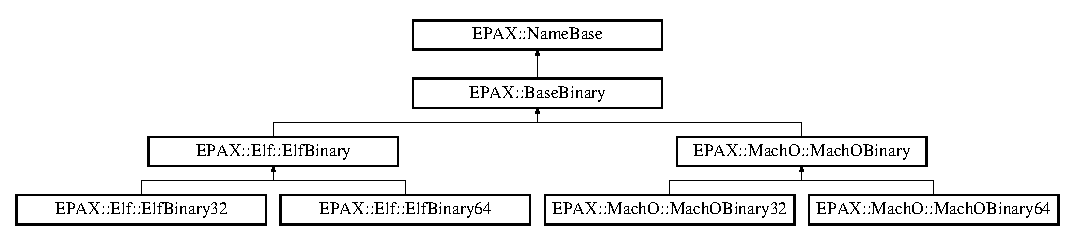
\includegraphics[height=2.786070cm]{class_e_p_a_x_1_1_base_binary}
\end{center}
\end{figure}
\subsection*{\-Public \-Member \-Functions}
\begin{DoxyCompactItemize}
\item 
\hyperlink{class_e_p_a_x_1_1_base_binary_ac58ab3c2bd58ffc732e5fa1a2b46e353}{\-Base\-Binary} (std\-::string n)
\item 
virtual \hyperlink{class_e_p_a_x_1_1_base_binary_a5d7991e869ded6715c7ddb68d5ce714b}{$\sim$\-Base\-Binary} ()
\item 
virtual \hyperlink{namespace_e_p_a_x_a4be639c006ef14def4708b37ee6dd67d}{\-Binary\-Format} \hyperlink{class_e_p_a_x_1_1_base_binary_a456741cd16605e5035ab89ab813f4373}{get\-Format} ()=0
\item 
virtual uint64\-\_\-t \hyperlink{class_e_p_a_x_1_1_base_binary_ad23fe3f3a6f5b387df2f4eb7e4a4f23d}{get\-Start\-Addr} ()=0
\item 
virtual void \hyperlink{class_e_p_a_x_1_1_base_binary_a8883d3b0580cae0f5a1960c6fbfd6a1f}{emit} (std\-::string n)=0
\item 
virtual bool \hyperlink{class_e_p_a_x_1_1_base_binary_a3e00d0fecc2defaab16a3ee4b72a32ca}{verify} ()=0
\item 
virtual bool \hyperlink{class_e_p_a_x_1_1_base_binary_ac544fc0d096ca8a555b30fe7126ae846}{is\-A\-R\-M} ()=0
\item 
virtual void \hyperlink{class_e_p_a_x_1_1_base_binary_a501175cac7fb1650bf378d6b4729c1ec}{describe} ()=0
\item 
virtual bool \hyperlink{class_e_p_a_x_1_1_base_binary_ac71bc6c28fe40456ddf626a8bbca257f}{is32\-Bit} ()=0
\item 
virtual bool \hyperlink{class_e_p_a_x_1_1_base_binary_a303cdafe0782ed63d8115bc225f169ee}{is64\-Bit} ()=0
\item 
virtual bool \hyperlink{class_e_p_a_x_1_1_base_binary_aeeb90ae234b0f661ef387ee31d3c4762}{is\-Executable} ()=0
\item 
virtual uint64\-\_\-t \hyperlink{class_e_p_a_x_1_1_base_binary_a3ebaa616622aaca98685ece5d59c05d8}{function\-End\-Address} (\hyperlink{class_e_p_a_x_1_1_function}{\-Function} $\ast$f, \hyperlink{class_e_p_a_x_1_1_function}{\-Function} $\ast$nextf)=0
\item 
uint32\-\_\-t \hyperlink{class_e_p_a_x_1_1_base_binary_ad13288de154013c2746bb08e3eedc935}{count\-Functions} ()
\item 
\hyperlink{class_e_p_a_x_1_1_function}{\-Function} $\ast$ \hyperlink{class_e_p_a_x_1_1_base_binary_a3c55ae83f63c176d8eddb3abb230e45a}{get\-First\-Function} ()
\item 
\hyperlink{class_e_p_a_x_1_1_function}{\-Function} $\ast$ \hyperlink{class_e_p_a_x_1_1_base_binary_a5ee395af9e7b93bb91798d15e8d21ce3}{get\-Next\-Function} (\hyperlink{class_e_p_a_x_1_1_function}{\-Function} $\ast$f)
\item 
bool \hyperlink{class_e_p_a_x_1_1_base_binary_a5a1956b1b159ac86cff862a4d74ee507}{is\-Last\-Function} (\hyperlink{class_e_p_a_x_1_1_function}{\-Function} $\ast$f)
\item 
\hyperlink{class_e_p_a_x_1_1_function}{\-Function} $\ast$ \hyperlink{class_e_p_a_x_1_1_base_binary_a2b97925db9ec8c520c4e1c18c8497a46}{find\-Function} (uint64\-\_\-t addr)
\item 
\hyperlink{class_e_p_a_x_1_1_input_file}{\-Input\-File} $\ast$ \hyperlink{class_e_p_a_x_1_1_base_binary_aeb9024c02d54cb2ce202d8387e636ddc}{get\-Input\-File} ()
\item 
virtual uint64\-\_\-t \hyperlink{class_e_p_a_x_1_1_base_binary_a1170c08c3540fdbfca516f4404de0c82}{get\-File\-Size} ()
\item 
virtual uint32\-\_\-t \hyperlink{class_e_p_a_x_1_1_base_binary_a50fc9adca69e89638154291291376dd7}{get\-I\-D} ()
\item 
virtual bool \hyperlink{class_e_p_a_x_1_1_base_binary_aa0f29bfa881c2199911465c64e421be6}{inside\-Text\-Range} (uint64\-\_\-t a)=0
\item 
virtual void \hyperlink{class_e_p_a_x_1_1_base_binary_a9ef8978bbd895a198b68cc04974c57cc}{print\-Sections} (std\-::ostream \&stream=std\-::cout)=0
\item 
virtual void \hyperlink{class_e_p_a_x_1_1_base_binary_a879d43acc68de4f468c26d5cfe4ab59d}{print\-Functions} (std\-::ostream \&stream=std\-::cout)=0
\end{DoxyCompactItemize}
\subsection*{\-Static \-Public \-Member \-Functions}
\begin{DoxyCompactItemize}
\item 
static const char $\ast$ \hyperlink{class_e_p_a_x_1_1_base_binary_a96e7dba2e794a751e8a462e1223bfc20}{get\-Format\-Name} (\hyperlink{namespace_e_p_a_x_a4be639c006ef14def4708b37ee6dd67d}{\-Binary\-Format} f)
\end{DoxyCompactItemize}
\subsection*{\-Protected \-Member \-Functions}
\begin{DoxyCompactItemize}
\item 
virtual void \hyperlink{class_e_p_a_x_1_1_base_binary_abcd76218158ab20a2f81d68a537b21cb}{find\-Functions} ()=0
\item 
void \hyperlink{class_e_p_a_x_1_1_base_binary_ad41eddf1063ab540878c90f788428aea}{lazy\-Functions} ()
\item 
virtual void \hyperlink{class_e_p_a_x_1_1_base_binary_adc22abd64f6a873fbce30c79508322fe}{find\-Symbols} ()=0
\item 
void \hyperlink{class_e_p_a_x_1_1_base_binary_aabbaef763d108e78d0d29c3bedbc0d35}{lazy\-Symbols} ()
\end{DoxyCompactItemize}
\subsection*{\-Protected \-Attributes}
\begin{DoxyCompactItemize}
\item 
\hyperlink{class_e_p_a_x_1_1_input_file}{\-Input\-File} $\ast$ \hyperlink{class_e_p_a_x_1_1_base_binary_a9e75692a1d1b71186a49dd77d8b74a65}{inputfile}
\item 
bool \hyperlink{class_e_p_a_x_1_1_base_binary_a3c83e522df1f2d99e5e0f81d7cd36fcc}{foundfunctions}
\item 
std\-::vector$<$ \hyperlink{class_e_p_a_x_1_1_function}{\-Function} $\ast$ $>$ $\ast$ \hyperlink{class_e_p_a_x_1_1_base_binary_aa26b782267daf58809b05047ff677a3e}{functions}
\item 
bool \hyperlink{class_e_p_a_x_1_1_base_binary_a941c0d2bd1b8fa811d8a516c603685af}{foundsymbols}
\item 
std\-::vector$<$ \hyperlink{class_e_p_a_x_1_1_symbol_table}{\-Symbol\-Table} $\ast$ $>$ $\ast$ \hyperlink{class_e_p_a_x_1_1_base_binary_ab2b5f8e146dba5f2f0ff32e34b6712bd}{symtabs}
\item 
std\-::vector$<$ \hyperlink{class_e_p_a_x_1_1_string_table}{\-String\-Table} $\ast$ $>$ $\ast$ \hyperlink{class_e_p_a_x_1_1_base_binary_a48e7fd1954b46f6bf7885dd70ae0ac78}{strtabs}
\end{DoxyCompactItemize}


\subsection{\-Detailed \-Description}


\-Definition at line 132 of file \-Base\-Class.\-hpp.



\subsection{\-Constructor \& \-Destructor \-Documentation}
\hypertarget{class_e_p_a_x_1_1_base_binary_ac58ab3c2bd58ffc732e5fa1a2b46e353}{\index{\-E\-P\-A\-X\-::\-Base\-Binary@{\-E\-P\-A\-X\-::\-Base\-Binary}!\-Base\-Binary@{\-Base\-Binary}}
\index{\-Base\-Binary@{\-Base\-Binary}!EPAX::BaseBinary@{\-E\-P\-A\-X\-::\-Base\-Binary}}
\subsubsection[{\-Base\-Binary}]{\setlength{\rightskip}{0pt plus 5cm}{\bf \-E\-P\-A\-X\-::\-Base\-Binary\-::\-Base\-Binary} (
\begin{DoxyParamCaption}
\item[{std\-::string}]{n}
\end{DoxyParamCaption}
)}}\label{class_e_p_a_x_1_1_base_binary_ac58ab3c2bd58ffc732e5fa1a2b46e353}


\-Definition at line 58 of file \-Base\-Class.\-cpp.

\hypertarget{class_e_p_a_x_1_1_base_binary_a5d7991e869ded6715c7ddb68d5ce714b}{\index{\-E\-P\-A\-X\-::\-Base\-Binary@{\-E\-P\-A\-X\-::\-Base\-Binary}!$\sim$\-Base\-Binary@{$\sim$\-Base\-Binary}}
\index{$\sim$\-Base\-Binary@{$\sim$\-Base\-Binary}!EPAX::BaseBinary@{\-E\-P\-A\-X\-::\-Base\-Binary}}
\subsubsection[{$\sim$\-Base\-Binary}]{\setlength{\rightskip}{0pt plus 5cm}{\bf \-E\-P\-A\-X\-::\-Base\-Binary\-::$\sim$\-Base\-Binary} (
\begin{DoxyParamCaption}
{}
\end{DoxyParamCaption}
)\hspace{0.3cm}{\ttfamily  \mbox{[}virtual\mbox{]}}}}\label{class_e_p_a_x_1_1_base_binary_a5d7991e869ded6715c7ddb68d5ce714b}


\-Definition at line 67 of file \-Base\-Class.\-cpp.



\subsection{\-Member \-Function \-Documentation}
\hypertarget{class_e_p_a_x_1_1_base_binary_ad13288de154013c2746bb08e3eedc935}{\index{\-E\-P\-A\-X\-::\-Base\-Binary@{\-E\-P\-A\-X\-::\-Base\-Binary}!count\-Functions@{count\-Functions}}
\index{count\-Functions@{count\-Functions}!EPAX::BaseBinary@{\-E\-P\-A\-X\-::\-Base\-Binary}}
\subsubsection[{count\-Functions}]{\setlength{\rightskip}{0pt plus 5cm}uint32\-\_\-t {\bf \-E\-P\-A\-X\-::\-Base\-Binary\-::count\-Functions} (
\begin{DoxyParamCaption}
{}
\end{DoxyParamCaption}
)}}\label{class_e_p_a_x_1_1_base_binary_ad13288de154013c2746bb08e3eedc935}


\-Definition at line 125 of file \-Base\-Class.\-cpp.

\hypertarget{class_e_p_a_x_1_1_base_binary_a501175cac7fb1650bf378d6b4729c1ec}{\index{\-E\-P\-A\-X\-::\-Base\-Binary@{\-E\-P\-A\-X\-::\-Base\-Binary}!describe@{describe}}
\index{describe@{describe}!EPAX::BaseBinary@{\-E\-P\-A\-X\-::\-Base\-Binary}}
\subsubsection[{describe}]{\setlength{\rightskip}{0pt plus 5cm}virtual void {\bf \-E\-P\-A\-X\-::\-Base\-Binary\-::describe} (
\begin{DoxyParamCaption}
{}
\end{DoxyParamCaption}
)\hspace{0.3cm}{\ttfamily  \mbox{[}pure virtual\mbox{]}}}}\label{class_e_p_a_x_1_1_base_binary_a501175cac7fb1650bf378d6b4729c1ec}


\-Implemented in \hyperlink{class_e_p_a_x_1_1_elf_1_1_elf_binary_aa6846ae0eedb4620e26e3b466efec629}{\-E\-P\-A\-X\-::\-Elf\-::\-Elf\-Binary}, and \hyperlink{class_e_p_a_x_1_1_mach_o_1_1_mach_o_binary_a7142994ba41ef1a5fad2d34e75278764}{\-E\-P\-A\-X\-::\-Mach\-O\-::\-Mach\-O\-Binary}.

\hypertarget{class_e_p_a_x_1_1_base_binary_a8883d3b0580cae0f5a1960c6fbfd6a1f}{\index{\-E\-P\-A\-X\-::\-Base\-Binary@{\-E\-P\-A\-X\-::\-Base\-Binary}!emit@{emit}}
\index{emit@{emit}!EPAX::BaseBinary@{\-E\-P\-A\-X\-::\-Base\-Binary}}
\subsubsection[{emit}]{\setlength{\rightskip}{0pt plus 5cm}virtual void {\bf \-E\-P\-A\-X\-::\-Base\-Binary\-::emit} (
\begin{DoxyParamCaption}
\item[{std\-::string}]{n}
\end{DoxyParamCaption}
)\hspace{0.3cm}{\ttfamily  \mbox{[}pure virtual\mbox{]}}}}\label{class_e_p_a_x_1_1_base_binary_a8883d3b0580cae0f5a1960c6fbfd6a1f}


\-Implemented in \hyperlink{class_e_p_a_x_1_1_elf_1_1_elf_binary_ac929a0c398ce61c8ac80df79dbb6a1d9}{\-E\-P\-A\-X\-::\-Elf\-::\-Elf\-Binary}, and \hyperlink{class_e_p_a_x_1_1_mach_o_1_1_mach_o_binary_a3a4b9b3138d22d2455fbddb4c694f532}{\-E\-P\-A\-X\-::\-Mach\-O\-::\-Mach\-O\-Binary}.

\hypertarget{class_e_p_a_x_1_1_base_binary_a2b97925db9ec8c520c4e1c18c8497a46}{\index{\-E\-P\-A\-X\-::\-Base\-Binary@{\-E\-P\-A\-X\-::\-Base\-Binary}!find\-Function@{find\-Function}}
\index{find\-Function@{find\-Function}!EPAX::BaseBinary@{\-E\-P\-A\-X\-::\-Base\-Binary}}
\subsubsection[{find\-Function}]{\setlength{\rightskip}{0pt plus 5cm}{\bf \-Function} $\ast$ {\bf \-E\-P\-A\-X\-::\-Base\-Binary\-::find\-Function} (
\begin{DoxyParamCaption}
\item[{uint64\-\_\-t}]{addr}
\end{DoxyParamCaption}
)}}\label{class_e_p_a_x_1_1_base_binary_a2b97925db9ec8c520c4e1c18c8497a46}


\-Definition at line 153 of file \-Base\-Class.\-cpp.

\hypertarget{class_e_p_a_x_1_1_base_binary_abcd76218158ab20a2f81d68a537b21cb}{\index{\-E\-P\-A\-X\-::\-Base\-Binary@{\-E\-P\-A\-X\-::\-Base\-Binary}!find\-Functions@{find\-Functions}}
\index{find\-Functions@{find\-Functions}!EPAX::BaseBinary@{\-E\-P\-A\-X\-::\-Base\-Binary}}
\subsubsection[{find\-Functions}]{\setlength{\rightskip}{0pt plus 5cm}virtual void {\bf \-E\-P\-A\-X\-::\-Base\-Binary\-::find\-Functions} (
\begin{DoxyParamCaption}
{}
\end{DoxyParamCaption}
)\hspace{0.3cm}{\ttfamily  \mbox{[}protected, pure virtual\mbox{]}}}}\label{class_e_p_a_x_1_1_base_binary_abcd76218158ab20a2f81d68a537b21cb}
\-Finds and internally stores all functions in the image

\begin{DoxyReturn}{\-Returns}
none 
\end{DoxyReturn}


\-Implemented in \hyperlink{class_e_p_a_x_1_1_elf_1_1_elf_binary_a57b3bc6b92a7964835e424d610523240}{\-E\-P\-A\-X\-::\-Elf\-::\-Elf\-Binary}, and \hyperlink{class_e_p_a_x_1_1_mach_o_1_1_mach_o_binary_a06e7ed071e394bd70b2a371b1360f591}{\-E\-P\-A\-X\-::\-Mach\-O\-::\-Mach\-O\-Binary}.

\hypertarget{class_e_p_a_x_1_1_base_binary_adc22abd64f6a873fbce30c79508322fe}{\index{\-E\-P\-A\-X\-::\-Base\-Binary@{\-E\-P\-A\-X\-::\-Base\-Binary}!find\-Symbols@{find\-Symbols}}
\index{find\-Symbols@{find\-Symbols}!EPAX::BaseBinary@{\-E\-P\-A\-X\-::\-Base\-Binary}}
\subsubsection[{find\-Symbols}]{\setlength{\rightskip}{0pt plus 5cm}virtual void {\bf \-E\-P\-A\-X\-::\-Base\-Binary\-::find\-Symbols} (
\begin{DoxyParamCaption}
{}
\end{DoxyParamCaption}
)\hspace{0.3cm}{\ttfamily  \mbox{[}protected, pure virtual\mbox{]}}}}\label{class_e_p_a_x_1_1_base_binary_adc22abd64f6a873fbce30c79508322fe}
\-Finds and internally stores all symbols in the image

\begin{DoxyReturn}{\-Returns}
none 
\end{DoxyReturn}


\-Implemented in \hyperlink{class_e_p_a_x_1_1_elf_1_1_elf_binary_a393e4e2eeea3224d1b61c6a8412c9da5}{\-E\-P\-A\-X\-::\-Elf\-::\-Elf\-Binary}, and \hyperlink{class_e_p_a_x_1_1_mach_o_1_1_mach_o_binary_a4c92ec8fe5a4c63d57b101f1e35f9291}{\-E\-P\-A\-X\-::\-Mach\-O\-::\-Mach\-O\-Binary}.

\hypertarget{class_e_p_a_x_1_1_base_binary_a3ebaa616622aaca98685ece5d59c05d8}{\index{\-E\-P\-A\-X\-::\-Base\-Binary@{\-E\-P\-A\-X\-::\-Base\-Binary}!function\-End\-Address@{function\-End\-Address}}
\index{function\-End\-Address@{function\-End\-Address}!EPAX::BaseBinary@{\-E\-P\-A\-X\-::\-Base\-Binary}}
\subsubsection[{function\-End\-Address}]{\setlength{\rightskip}{0pt plus 5cm}virtual uint64\-\_\-t {\bf \-E\-P\-A\-X\-::\-Base\-Binary\-::function\-End\-Address} (
\begin{DoxyParamCaption}
\item[{{\bf \-Function} $\ast$}]{f, }
\item[{{\bf \-Function} $\ast$}]{nextf}
\end{DoxyParamCaption}
)\hspace{0.3cm}{\ttfamily  \mbox{[}pure virtual\mbox{]}}}}\label{class_e_p_a_x_1_1_base_binary_a3ebaa616622aaca98685ece5d59c05d8}


\-Implemented in \hyperlink{class_e_p_a_x_1_1_elf_1_1_elf_binary_a7cba4b5796d98043e281f46437abb6d9}{\-E\-P\-A\-X\-::\-Elf\-::\-Elf\-Binary}, and \hyperlink{class_e_p_a_x_1_1_mach_o_1_1_mach_o_binary_a5b58a3105ffe8aff09dc2c20421e8744}{\-E\-P\-A\-X\-::\-Mach\-O\-::\-Mach\-O\-Binary}.

\hypertarget{class_e_p_a_x_1_1_base_binary_a1170c08c3540fdbfca516f4404de0c82}{\index{\-E\-P\-A\-X\-::\-Base\-Binary@{\-E\-P\-A\-X\-::\-Base\-Binary}!get\-File\-Size@{get\-File\-Size}}
\index{get\-File\-Size@{get\-File\-Size}!EPAX::BaseBinary@{\-E\-P\-A\-X\-::\-Base\-Binary}}
\subsubsection[{get\-File\-Size}]{\setlength{\rightskip}{0pt plus 5cm}uint64\-\_\-t {\bf \-E\-P\-A\-X\-::\-Base\-Binary\-::get\-File\-Size} (
\begin{DoxyParamCaption}
{}
\end{DoxyParamCaption}
)\hspace{0.3cm}{\ttfamily  \mbox{[}virtual\mbox{]}}}}\label{class_e_p_a_x_1_1_base_binary_a1170c08c3540fdbfca516f4404de0c82}


\-Definition at line 149 of file \-Base\-Class.\-cpp.

\hypertarget{class_e_p_a_x_1_1_base_binary_a3c55ae83f63c176d8eddb3abb230e45a}{\index{\-E\-P\-A\-X\-::\-Base\-Binary@{\-E\-P\-A\-X\-::\-Base\-Binary}!get\-First\-Function@{get\-First\-Function}}
\index{get\-First\-Function@{get\-First\-Function}!EPAX::BaseBinary@{\-E\-P\-A\-X\-::\-Base\-Binary}}
\subsubsection[{get\-First\-Function}]{\setlength{\rightskip}{0pt plus 5cm}{\bf \-Function} $\ast$ {\bf \-E\-P\-A\-X\-::\-Base\-Binary\-::get\-First\-Function} (
\begin{DoxyParamCaption}
{}
\end{DoxyParamCaption}
)}}\label{class_e_p_a_x_1_1_base_binary_a3c55ae83f63c176d8eddb3abb230e45a}


\-Definition at line 115 of file \-Base\-Class.\-cpp.

\hypertarget{class_e_p_a_x_1_1_base_binary_a456741cd16605e5035ab89ab813f4373}{\index{\-E\-P\-A\-X\-::\-Base\-Binary@{\-E\-P\-A\-X\-::\-Base\-Binary}!get\-Format@{get\-Format}}
\index{get\-Format@{get\-Format}!EPAX::BaseBinary@{\-E\-P\-A\-X\-::\-Base\-Binary}}
\subsubsection[{get\-Format}]{\setlength{\rightskip}{0pt plus 5cm}virtual {\bf \-Binary\-Format} {\bf \-E\-P\-A\-X\-::\-Base\-Binary\-::get\-Format} (
\begin{DoxyParamCaption}
{}
\end{DoxyParamCaption}
)\hspace{0.3cm}{\ttfamily  \mbox{[}pure virtual\mbox{]}}}}\label{class_e_p_a_x_1_1_base_binary_a456741cd16605e5035ab89ab813f4373}


\-Implemented in \hyperlink{class_e_p_a_x_1_1_elf_1_1_elf_binary64_a8d4ac63ef8a488fb6ad98fd24ad36d07}{\-E\-P\-A\-X\-::\-Elf\-::\-Elf\-Binary64}, \hyperlink{class_e_p_a_x_1_1_elf_1_1_elf_binary32_ad3c232fe03109e9a59e5456420d4fed3}{\-E\-P\-A\-X\-::\-Elf\-::\-Elf\-Binary32}, \hyperlink{class_e_p_a_x_1_1_mach_o_1_1_mach_o_binary64_ab2aa03d22ba0339c415a9dc9e6a0912b}{\-E\-P\-A\-X\-::\-Mach\-O\-::\-Mach\-O\-Binary64}, \hyperlink{class_e_p_a_x_1_1_mach_o_1_1_mach_o_binary32_a37eab3a09ee0f670f2633a56c890100e}{\-E\-P\-A\-X\-::\-Mach\-O\-::\-Mach\-O\-Binary32}, \hyperlink{class_e_p_a_x_1_1_elf_1_1_elf_binary_a2f8cfe8d4567e4aefbeb0717da3f0e9c}{\-E\-P\-A\-X\-::\-Elf\-::\-Elf\-Binary}, and \hyperlink{class_e_p_a_x_1_1_mach_o_1_1_mach_o_binary_a435106c1f40d1ec16ac539fbdecd88bd}{\-E\-P\-A\-X\-::\-Mach\-O\-::\-Mach\-O\-Binary}.

\hypertarget{class_e_p_a_x_1_1_base_binary_a96e7dba2e794a751e8a462e1223bfc20}{\index{\-E\-P\-A\-X\-::\-Base\-Binary@{\-E\-P\-A\-X\-::\-Base\-Binary}!get\-Format\-Name@{get\-Format\-Name}}
\index{get\-Format\-Name@{get\-Format\-Name}!EPAX::BaseBinary@{\-E\-P\-A\-X\-::\-Base\-Binary}}
\subsubsection[{get\-Format\-Name}]{\setlength{\rightskip}{0pt plus 5cm}const char $\ast$ {\bf \-E\-P\-A\-X\-::\-Base\-Binary\-::get\-Format\-Name} (
\begin{DoxyParamCaption}
\item[{{\bf \-Binary\-Format}}]{f}
\end{DoxyParamCaption}
)\hspace{0.3cm}{\ttfamily  \mbox{[}static\mbox{]}}}}\label{class_e_p_a_x_1_1_base_binary_a96e7dba2e794a751e8a462e1223bfc20}


\-Definition at line 98 of file \-Base\-Class.\-cpp.

\hypertarget{class_e_p_a_x_1_1_base_binary_a50fc9adca69e89638154291291376dd7}{\index{\-E\-P\-A\-X\-::\-Base\-Binary@{\-E\-P\-A\-X\-::\-Base\-Binary}!get\-I\-D@{get\-I\-D}}
\index{get\-I\-D@{get\-I\-D}!EPAX::BaseBinary@{\-E\-P\-A\-X\-::\-Base\-Binary}}
\subsubsection[{get\-I\-D}]{\setlength{\rightskip}{0pt plus 5cm}virtual uint32\-\_\-t {\bf \-E\-P\-A\-X\-::\-Base\-Binary\-::get\-I\-D} (
\begin{DoxyParamCaption}
{}
\end{DoxyParamCaption}
)\hspace{0.3cm}{\ttfamily  \mbox{[}inline, virtual\mbox{]}}}}\label{class_e_p_a_x_1_1_base_binary_a50fc9adca69e89638154291291376dd7}


\-Definition at line 190 of file \-Base\-Class.\-hpp.

\hypertarget{class_e_p_a_x_1_1_base_binary_aeb9024c02d54cb2ce202d8387e636ddc}{\index{\-E\-P\-A\-X\-::\-Base\-Binary@{\-E\-P\-A\-X\-::\-Base\-Binary}!get\-Input\-File@{get\-Input\-File}}
\index{get\-Input\-File@{get\-Input\-File}!EPAX::BaseBinary@{\-E\-P\-A\-X\-::\-Base\-Binary}}
\subsubsection[{get\-Input\-File}]{\setlength{\rightskip}{0pt plus 5cm}{\bf \-Input\-File}$\ast$ {\bf \-E\-P\-A\-X\-::\-Base\-Binary\-::get\-Input\-File} (
\begin{DoxyParamCaption}
{}
\end{DoxyParamCaption}
)\hspace{0.3cm}{\ttfamily  \mbox{[}inline\mbox{]}}}}\label{class_e_p_a_x_1_1_base_binary_aeb9024c02d54cb2ce202d8387e636ddc}


\-Definition at line 186 of file \-Base\-Class.\-hpp.

\hypertarget{class_e_p_a_x_1_1_base_binary_a5ee395af9e7b93bb91798d15e8d21ce3}{\index{\-E\-P\-A\-X\-::\-Base\-Binary@{\-E\-P\-A\-X\-::\-Base\-Binary}!get\-Next\-Function@{get\-Next\-Function}}
\index{get\-Next\-Function@{get\-Next\-Function}!EPAX::BaseBinary@{\-E\-P\-A\-X\-::\-Base\-Binary}}
\subsubsection[{get\-Next\-Function}]{\setlength{\rightskip}{0pt plus 5cm}{\bf \-Function} $\ast$ {\bf \-E\-P\-A\-X\-::\-Base\-Binary\-::get\-Next\-Function} (
\begin{DoxyParamCaption}
\item[{{\bf \-Function} $\ast$}]{f}
\end{DoxyParamCaption}
)}}\label{class_e_p_a_x_1_1_base_binary_a5ee395af9e7b93bb91798d15e8d21ce3}


\-Definition at line 130 of file \-Base\-Class.\-cpp.

\hypertarget{class_e_p_a_x_1_1_base_binary_ad23fe3f3a6f5b387df2f4eb7e4a4f23d}{\index{\-E\-P\-A\-X\-::\-Base\-Binary@{\-E\-P\-A\-X\-::\-Base\-Binary}!get\-Start\-Addr@{get\-Start\-Addr}}
\index{get\-Start\-Addr@{get\-Start\-Addr}!EPAX::BaseBinary@{\-E\-P\-A\-X\-::\-Base\-Binary}}
\subsubsection[{get\-Start\-Addr}]{\setlength{\rightskip}{0pt plus 5cm}virtual uint64\-\_\-t {\bf \-E\-P\-A\-X\-::\-Base\-Binary\-::get\-Start\-Addr} (
\begin{DoxyParamCaption}
{}
\end{DoxyParamCaption}
)\hspace{0.3cm}{\ttfamily  \mbox{[}pure virtual\mbox{]}}}}\label{class_e_p_a_x_1_1_base_binary_ad23fe3f3a6f5b387df2f4eb7e4a4f23d}


\-Implemented in \hyperlink{class_e_p_a_x_1_1_elf_1_1_elf_binary_af4d56ab5e4f25b17f236c1712dd7c2bb}{\-E\-P\-A\-X\-::\-Elf\-::\-Elf\-Binary}, and \hyperlink{class_e_p_a_x_1_1_mach_o_1_1_mach_o_binary_a426e6fdd744908571c46e10608211df4}{\-E\-P\-A\-X\-::\-Mach\-O\-::\-Mach\-O\-Binary}.

\hypertarget{class_e_p_a_x_1_1_base_binary_aa0f29bfa881c2199911465c64e421be6}{\index{\-E\-P\-A\-X\-::\-Base\-Binary@{\-E\-P\-A\-X\-::\-Base\-Binary}!inside\-Text\-Range@{inside\-Text\-Range}}
\index{inside\-Text\-Range@{inside\-Text\-Range}!EPAX::BaseBinary@{\-E\-P\-A\-X\-::\-Base\-Binary}}
\subsubsection[{inside\-Text\-Range}]{\setlength{\rightskip}{0pt plus 5cm}virtual bool {\bf \-E\-P\-A\-X\-::\-Base\-Binary\-::inside\-Text\-Range} (
\begin{DoxyParamCaption}
\item[{uint64\-\_\-t}]{a}
\end{DoxyParamCaption}
)\hspace{0.3cm}{\ttfamily  \mbox{[}pure virtual\mbox{]}}}}\label{class_e_p_a_x_1_1_base_binary_aa0f29bfa881c2199911465c64e421be6}


\-Implemented in \hyperlink{class_e_p_a_x_1_1_elf_1_1_elf_binary_ae52abd95dd6d7f77d3e6da0e629c86e5}{\-E\-P\-A\-X\-::\-Elf\-::\-Elf\-Binary}, and \hyperlink{class_e_p_a_x_1_1_mach_o_1_1_mach_o_binary_a37bd8cd22a68dc0fe4836c5781568725}{\-E\-P\-A\-X\-::\-Mach\-O\-::\-Mach\-O\-Binary}.

\hypertarget{class_e_p_a_x_1_1_base_binary_ac71bc6c28fe40456ddf626a8bbca257f}{\index{\-E\-P\-A\-X\-::\-Base\-Binary@{\-E\-P\-A\-X\-::\-Base\-Binary}!is32\-Bit@{is32\-Bit}}
\index{is32\-Bit@{is32\-Bit}!EPAX::BaseBinary@{\-E\-P\-A\-X\-::\-Base\-Binary}}
\subsubsection[{is32\-Bit}]{\setlength{\rightskip}{0pt plus 5cm}virtual bool {\bf \-E\-P\-A\-X\-::\-Base\-Binary\-::is32\-Bit} (
\begin{DoxyParamCaption}
{}
\end{DoxyParamCaption}
)\hspace{0.3cm}{\ttfamily  \mbox{[}pure virtual\mbox{]}}}}\label{class_e_p_a_x_1_1_base_binary_ac71bc6c28fe40456ddf626a8bbca257f}


\-Implemented in \hyperlink{class_e_p_a_x_1_1_elf_1_1_elf_binary_a813a2985bd91b6e7640a2221235fdb4e}{\-E\-P\-A\-X\-::\-Elf\-::\-Elf\-Binary}, and \hyperlink{class_e_p_a_x_1_1_mach_o_1_1_mach_o_binary_a6c3c547d72fe13a51b702fcfc6c1c271}{\-E\-P\-A\-X\-::\-Mach\-O\-::\-Mach\-O\-Binary}.

\hypertarget{class_e_p_a_x_1_1_base_binary_a303cdafe0782ed63d8115bc225f169ee}{\index{\-E\-P\-A\-X\-::\-Base\-Binary@{\-E\-P\-A\-X\-::\-Base\-Binary}!is64\-Bit@{is64\-Bit}}
\index{is64\-Bit@{is64\-Bit}!EPAX::BaseBinary@{\-E\-P\-A\-X\-::\-Base\-Binary}}
\subsubsection[{is64\-Bit}]{\setlength{\rightskip}{0pt plus 5cm}virtual bool {\bf \-E\-P\-A\-X\-::\-Base\-Binary\-::is64\-Bit} (
\begin{DoxyParamCaption}
{}
\end{DoxyParamCaption}
)\hspace{0.3cm}{\ttfamily  \mbox{[}pure virtual\mbox{]}}}}\label{class_e_p_a_x_1_1_base_binary_a303cdafe0782ed63d8115bc225f169ee}


\-Implemented in \hyperlink{class_e_p_a_x_1_1_elf_1_1_elf_binary_a07de5ed756446ede40d3f1328eedfa0b}{\-E\-P\-A\-X\-::\-Elf\-::\-Elf\-Binary}, and \hyperlink{class_e_p_a_x_1_1_mach_o_1_1_mach_o_binary_a892a753783fa1feaa3f98fcad476da8a}{\-E\-P\-A\-X\-::\-Mach\-O\-::\-Mach\-O\-Binary}.

\hypertarget{class_e_p_a_x_1_1_base_binary_ac544fc0d096ca8a555b30fe7126ae846}{\index{\-E\-P\-A\-X\-::\-Base\-Binary@{\-E\-P\-A\-X\-::\-Base\-Binary}!is\-A\-R\-M@{is\-A\-R\-M}}
\index{is\-A\-R\-M@{is\-A\-R\-M}!EPAX::BaseBinary@{\-E\-P\-A\-X\-::\-Base\-Binary}}
\subsubsection[{is\-A\-R\-M}]{\setlength{\rightskip}{0pt plus 5cm}virtual bool {\bf \-E\-P\-A\-X\-::\-Base\-Binary\-::is\-A\-R\-M} (
\begin{DoxyParamCaption}
{}
\end{DoxyParamCaption}
)\hspace{0.3cm}{\ttfamily  \mbox{[}pure virtual\mbox{]}}}}\label{class_e_p_a_x_1_1_base_binary_ac544fc0d096ca8a555b30fe7126ae846}


\-Implemented in \hyperlink{class_e_p_a_x_1_1_elf_1_1_elf_binary_a48ca78d2f324eef54c478532d1d38636}{\-E\-P\-A\-X\-::\-Elf\-::\-Elf\-Binary}, and \hyperlink{class_e_p_a_x_1_1_mach_o_1_1_mach_o_binary_a7d857ef9a99dc9d553e7e764234db957}{\-E\-P\-A\-X\-::\-Mach\-O\-::\-Mach\-O\-Binary}.

\hypertarget{class_e_p_a_x_1_1_base_binary_aeeb90ae234b0f661ef387ee31d3c4762}{\index{\-E\-P\-A\-X\-::\-Base\-Binary@{\-E\-P\-A\-X\-::\-Base\-Binary}!is\-Executable@{is\-Executable}}
\index{is\-Executable@{is\-Executable}!EPAX::BaseBinary@{\-E\-P\-A\-X\-::\-Base\-Binary}}
\subsubsection[{is\-Executable}]{\setlength{\rightskip}{0pt plus 5cm}virtual bool {\bf \-E\-P\-A\-X\-::\-Base\-Binary\-::is\-Executable} (
\begin{DoxyParamCaption}
{}
\end{DoxyParamCaption}
)\hspace{0.3cm}{\ttfamily  \mbox{[}pure virtual\mbox{]}}}}\label{class_e_p_a_x_1_1_base_binary_aeeb90ae234b0f661ef387ee31d3c4762}


\-Implemented in \hyperlink{class_e_p_a_x_1_1_elf_1_1_elf_binary_a683bf66639d6fb4c4d9e9904a563494e}{\-E\-P\-A\-X\-::\-Elf\-::\-Elf\-Binary}, and \hyperlink{class_e_p_a_x_1_1_mach_o_1_1_mach_o_binary_a6031c2f4420ec57b008d33a27f490a51}{\-E\-P\-A\-X\-::\-Mach\-O\-::\-Mach\-O\-Binary}.

\hypertarget{class_e_p_a_x_1_1_base_binary_a5a1956b1b159ac86cff862a4d74ee507}{\index{\-E\-P\-A\-X\-::\-Base\-Binary@{\-E\-P\-A\-X\-::\-Base\-Binary}!is\-Last\-Function@{is\-Last\-Function}}
\index{is\-Last\-Function@{is\-Last\-Function}!EPAX::BaseBinary@{\-E\-P\-A\-X\-::\-Base\-Binary}}
\subsubsection[{is\-Last\-Function}]{\setlength{\rightskip}{0pt plus 5cm}bool {\bf \-E\-P\-A\-X\-::\-Base\-Binary\-::is\-Last\-Function} (
\begin{DoxyParamCaption}
\item[{{\bf \-Function} $\ast$}]{f}
\end{DoxyParamCaption}
)}}\label{class_e_p_a_x_1_1_base_binary_a5a1956b1b159ac86cff862a4d74ee507}


\-Definition at line 138 of file \-Base\-Class.\-cpp.

\hypertarget{class_e_p_a_x_1_1_base_binary_ad41eddf1063ab540878c90f788428aea}{\index{\-E\-P\-A\-X\-::\-Base\-Binary@{\-E\-P\-A\-X\-::\-Base\-Binary}!lazy\-Functions@{lazy\-Functions}}
\index{lazy\-Functions@{lazy\-Functions}!EPAX::BaseBinary@{\-E\-P\-A\-X\-::\-Base\-Binary}}
\subsubsection[{lazy\-Functions}]{\setlength{\rightskip}{0pt plus 5cm}void {\bf \-E\-P\-A\-X\-::\-Base\-Binary\-::lazy\-Functions} (
\begin{DoxyParamCaption}
{}
\end{DoxyParamCaption}
)\hspace{0.3cm}{\ttfamily  \mbox{[}protected\mbox{]}}}}\label{class_e_p_a_x_1_1_base_binary_ad41eddf1063ab540878c90f788428aea}


\-Definition at line 103 of file \-Base\-Class.\-cpp.

\hypertarget{class_e_p_a_x_1_1_base_binary_aabbaef763d108e78d0d29c3bedbc0d35}{\index{\-E\-P\-A\-X\-::\-Base\-Binary@{\-E\-P\-A\-X\-::\-Base\-Binary}!lazy\-Symbols@{lazy\-Symbols}}
\index{lazy\-Symbols@{lazy\-Symbols}!EPAX::BaseBinary@{\-E\-P\-A\-X\-::\-Base\-Binary}}
\subsubsection[{lazy\-Symbols}]{\setlength{\rightskip}{0pt plus 5cm}void {\bf \-E\-P\-A\-X\-::\-Base\-Binary\-::lazy\-Symbols} (
\begin{DoxyParamCaption}
{}
\end{DoxyParamCaption}
)\hspace{0.3cm}{\ttfamily  \mbox{[}protected\mbox{]}}}}\label{class_e_p_a_x_1_1_base_binary_aabbaef763d108e78d0d29c3bedbc0d35}


\-Definition at line 109 of file \-Base\-Class.\-cpp.

\hypertarget{class_e_p_a_x_1_1_base_binary_a879d43acc68de4f468c26d5cfe4ab59d}{\index{\-E\-P\-A\-X\-::\-Base\-Binary@{\-E\-P\-A\-X\-::\-Base\-Binary}!print\-Functions@{print\-Functions}}
\index{print\-Functions@{print\-Functions}!EPAX::BaseBinary@{\-E\-P\-A\-X\-::\-Base\-Binary}}
\subsubsection[{print\-Functions}]{\setlength{\rightskip}{0pt plus 5cm}virtual void {\bf \-E\-P\-A\-X\-::\-Base\-Binary\-::print\-Functions} (
\begin{DoxyParamCaption}
\item[{std\-::ostream \&}]{stream = {\ttfamily std\-:\-:cout}}
\end{DoxyParamCaption}
)\hspace{0.3cm}{\ttfamily  \mbox{[}pure virtual\mbox{]}}}}\label{class_e_p_a_x_1_1_base_binary_a879d43acc68de4f468c26d5cfe4ab59d}


\-Implemented in \hyperlink{class_e_p_a_x_1_1_elf_1_1_elf_binary_aac1eb1e8571502f6005ac54d4b6e5920}{\-E\-P\-A\-X\-::\-Elf\-::\-Elf\-Binary}, and \hyperlink{class_e_p_a_x_1_1_mach_o_1_1_mach_o_binary_ad6b3af54bfd54fa0f37f22efc94fc985}{\-E\-P\-A\-X\-::\-Mach\-O\-::\-Mach\-O\-Binary}.

\hypertarget{class_e_p_a_x_1_1_base_binary_a9ef8978bbd895a198b68cc04974c57cc}{\index{\-E\-P\-A\-X\-::\-Base\-Binary@{\-E\-P\-A\-X\-::\-Base\-Binary}!print\-Sections@{print\-Sections}}
\index{print\-Sections@{print\-Sections}!EPAX::BaseBinary@{\-E\-P\-A\-X\-::\-Base\-Binary}}
\subsubsection[{print\-Sections}]{\setlength{\rightskip}{0pt plus 5cm}virtual void {\bf \-E\-P\-A\-X\-::\-Base\-Binary\-::print\-Sections} (
\begin{DoxyParamCaption}
\item[{std\-::ostream \&}]{stream = {\ttfamily std\-:\-:cout}}
\end{DoxyParamCaption}
)\hspace{0.3cm}{\ttfamily  \mbox{[}pure virtual\mbox{]}}}}\label{class_e_p_a_x_1_1_base_binary_a9ef8978bbd895a198b68cc04974c57cc}


\-Implemented in \hyperlink{class_e_p_a_x_1_1_elf_1_1_elf_binary_ae200e871cf5c040ed1d8ed074eb1e5c2}{\-E\-P\-A\-X\-::\-Elf\-::\-Elf\-Binary}, and \hyperlink{class_e_p_a_x_1_1_mach_o_1_1_mach_o_binary_a654a69dcd9a459f5e78b740047b94fa0}{\-E\-P\-A\-X\-::\-Mach\-O\-::\-Mach\-O\-Binary}.

\hypertarget{class_e_p_a_x_1_1_base_binary_a3e00d0fecc2defaab16a3ee4b72a32ca}{\index{\-E\-P\-A\-X\-::\-Base\-Binary@{\-E\-P\-A\-X\-::\-Base\-Binary}!verify@{verify}}
\index{verify@{verify}!EPAX::BaseBinary@{\-E\-P\-A\-X\-::\-Base\-Binary}}
\subsubsection[{verify}]{\setlength{\rightskip}{0pt plus 5cm}virtual bool {\bf \-E\-P\-A\-X\-::\-Base\-Binary\-::verify} (
\begin{DoxyParamCaption}
{}
\end{DoxyParamCaption}
)\hspace{0.3cm}{\ttfamily  \mbox{[}pure virtual\mbox{]}}}}\label{class_e_p_a_x_1_1_base_binary_a3e00d0fecc2defaab16a3ee4b72a32ca}


\-Implemented in \hyperlink{class_e_p_a_x_1_1_elf_1_1_elf_binary_a9955c801d73bcc62ce60a884f4d36464}{\-E\-P\-A\-X\-::\-Elf\-::\-Elf\-Binary}, and \hyperlink{class_e_p_a_x_1_1_mach_o_1_1_mach_o_binary_aa0eb9a16309170238ca0d3cc027a116b}{\-E\-P\-A\-X\-::\-Mach\-O\-::\-Mach\-O\-Binary}.



\subsection{\-Member \-Data \-Documentation}
\hypertarget{class_e_p_a_x_1_1_base_binary_a3c83e522df1f2d99e5e0f81d7cd36fcc}{\index{\-E\-P\-A\-X\-::\-Base\-Binary@{\-E\-P\-A\-X\-::\-Base\-Binary}!foundfunctions@{foundfunctions}}
\index{foundfunctions@{foundfunctions}!EPAX::BaseBinary@{\-E\-P\-A\-X\-::\-Base\-Binary}}
\subsubsection[{foundfunctions}]{\setlength{\rightskip}{0pt plus 5cm}bool {\bf \-E\-P\-A\-X\-::\-Base\-Binary\-::foundfunctions}\hspace{0.3cm}{\ttfamily  \mbox{[}protected\mbox{]}}}}\label{class_e_p_a_x_1_1_base_binary_a3c83e522df1f2d99e5e0f81d7cd36fcc}


\-Definition at line 147 of file \-Base\-Class.\-hpp.

\hypertarget{class_e_p_a_x_1_1_base_binary_a941c0d2bd1b8fa811d8a516c603685af}{\index{\-E\-P\-A\-X\-::\-Base\-Binary@{\-E\-P\-A\-X\-::\-Base\-Binary}!foundsymbols@{foundsymbols}}
\index{foundsymbols@{foundsymbols}!EPAX::BaseBinary@{\-E\-P\-A\-X\-::\-Base\-Binary}}
\subsubsection[{foundsymbols}]{\setlength{\rightskip}{0pt plus 5cm}bool {\bf \-E\-P\-A\-X\-::\-Base\-Binary\-::foundsymbols}\hspace{0.3cm}{\ttfamily  \mbox{[}protected\mbox{]}}}}\label{class_e_p_a_x_1_1_base_binary_a941c0d2bd1b8fa811d8a516c603685af}


\-Definition at line 157 of file \-Base\-Class.\-hpp.

\hypertarget{class_e_p_a_x_1_1_base_binary_aa26b782267daf58809b05047ff677a3e}{\index{\-E\-P\-A\-X\-::\-Base\-Binary@{\-E\-P\-A\-X\-::\-Base\-Binary}!functions@{functions}}
\index{functions@{functions}!EPAX::BaseBinary@{\-E\-P\-A\-X\-::\-Base\-Binary}}
\subsubsection[{functions}]{\setlength{\rightskip}{0pt plus 5cm}std\-::vector$<${\bf \-Function}$\ast$$>$$\ast$ {\bf \-E\-P\-A\-X\-::\-Base\-Binary\-::functions}\hspace{0.3cm}{\ttfamily  \mbox{[}protected\mbox{]}}}}\label{class_e_p_a_x_1_1_base_binary_aa26b782267daf58809b05047ff677a3e}


\-Definition at line 148 of file \-Base\-Class.\-hpp.

\hypertarget{class_e_p_a_x_1_1_base_binary_a9e75692a1d1b71186a49dd77d8b74a65}{\index{\-E\-P\-A\-X\-::\-Base\-Binary@{\-E\-P\-A\-X\-::\-Base\-Binary}!inputfile@{inputfile}}
\index{inputfile@{inputfile}!EPAX::BaseBinary@{\-E\-P\-A\-X\-::\-Base\-Binary}}
\subsubsection[{inputfile}]{\setlength{\rightskip}{0pt plus 5cm}{\bf \-Input\-File}$\ast$ {\bf \-E\-P\-A\-X\-::\-Base\-Binary\-::inputfile}\hspace{0.3cm}{\ttfamily  \mbox{[}protected\mbox{]}}}}\label{class_e_p_a_x_1_1_base_binary_a9e75692a1d1b71186a49dd77d8b74a65}
\-The image file 

\-Definition at line 138 of file \-Base\-Class.\-hpp.

\hypertarget{class_e_p_a_x_1_1_base_binary_a48e7fd1954b46f6bf7885dd70ae0ac78}{\index{\-E\-P\-A\-X\-::\-Base\-Binary@{\-E\-P\-A\-X\-::\-Base\-Binary}!strtabs@{strtabs}}
\index{strtabs@{strtabs}!EPAX::BaseBinary@{\-E\-P\-A\-X\-::\-Base\-Binary}}
\subsubsection[{strtabs}]{\setlength{\rightskip}{0pt plus 5cm}std\-::vector$<${\bf \-String\-Table}$\ast$$>$$\ast$ {\bf \-E\-P\-A\-X\-::\-Base\-Binary\-::strtabs}\hspace{0.3cm}{\ttfamily  \mbox{[}protected\mbox{]}}}}\label{class_e_p_a_x_1_1_base_binary_a48e7fd1954b46f6bf7885dd70ae0ac78}


\-Definition at line 159 of file \-Base\-Class.\-hpp.

\hypertarget{class_e_p_a_x_1_1_base_binary_ab2b5f8e146dba5f2f0ff32e34b6712bd}{\index{\-E\-P\-A\-X\-::\-Base\-Binary@{\-E\-P\-A\-X\-::\-Base\-Binary}!symtabs@{symtabs}}
\index{symtabs@{symtabs}!EPAX::BaseBinary@{\-E\-P\-A\-X\-::\-Base\-Binary}}
\subsubsection[{symtabs}]{\setlength{\rightskip}{0pt plus 5cm}std\-::vector$<${\bf \-Symbol\-Table}$\ast$$>$$\ast$ {\bf \-E\-P\-A\-X\-::\-Base\-Binary\-::symtabs}\hspace{0.3cm}{\ttfamily  \mbox{[}protected\mbox{]}}}}\label{class_e_p_a_x_1_1_base_binary_ab2b5f8e146dba5f2f0ff32e34b6712bd}


\-Definition at line 158 of file \-Base\-Class.\-hpp.



\-The documentation for this class was generated from the following files\-:\begin{DoxyCompactItemize}
\item 
\hyperlink{_base_class_8hpp}{\-Base\-Class.\-hpp}\item 
\hyperlink{_base_class_8cpp}{\-Base\-Class.\-cpp}\end{DoxyCompactItemize}

\hypertarget{class_e_p_a_x_1_1_basic_block}{\section{\-E\-P\-A\-X\-:\-:\-Basic\-Block \-Class \-Reference}
\label{class_e_p_a_x_1_1_basic_block}\index{\-E\-P\-A\-X\-::\-Basic\-Block@{\-E\-P\-A\-X\-::\-Basic\-Block}}
}


{\ttfamily \#include $<$\-Basic\-Block.\-hpp$>$}

\-Inheritance diagram for \-E\-P\-A\-X\-:\-:\-Basic\-Block\-:\begin{figure}[H]
\begin{center}
\leavevmode
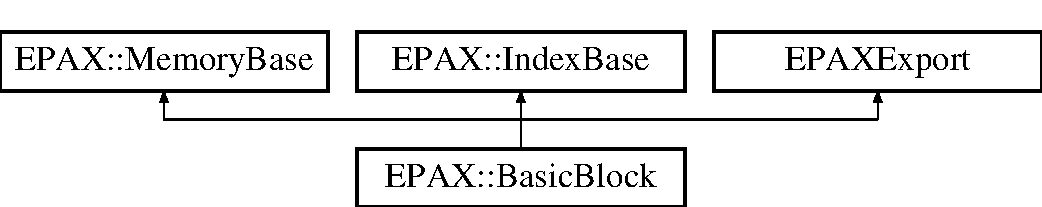
\includegraphics[height=2.000000cm]{class_e_p_a_x_1_1_basic_block}
\end{center}
\end{figure}
\subsection*{\-Public \-Member \-Functions}
\begin{DoxyCompactItemize}
\item 
\hyperlink{class_e_p_a_x_1_1_basic_block_adf527ffb872f3969f891d6506973fac7}{\-Basic\-Block} (\hyperlink{class_e_p_a_x_1_1_function}{\-Function} $\ast$f, uint64\-\_\-t a, uint32\-\_\-t i)
\item 
virtual \hyperlink{class_e_p_a_x_1_1_basic_block_ad142c305b9158af0a3eb0d7dceb95b3f}{$\sim$\-Basic\-Block} ()
\item 
uint32\-\_\-t \hyperlink{class_e_p_a_x_1_1_basic_block_a72cd48f6ceb9f2d0085ff56b6936f21d}{count\-Instructions} ()
\item 
void \hyperlink{class_e_p_a_x_1_1_basic_block_a113ee43c4b6d28faabc9a07cd6ffdbef}{add\-Instruction} (\hyperlink{class_e_p_a_x_1_1_instruction}{\-Instruction} $\ast$insn)
\item 
\hyperlink{class_e_p_a_x_1_1_instruction}{\-Instruction} $\ast$ \hyperlink{class_e_p_a_x_1_1_basic_block_af786852087748a3b29b562936da3e8ba}{get\-Instruction} (uint32\-\_\-t idx)
\item 
\hyperlink{class_e_p_a_x_1_1_instruction}{\-Instruction} $\ast$ \hyperlink{class_e_p_a_x_1_1_basic_block_ac27e14d15376e0741deb54ad108f8c32}{head} ()
\item 
\hyperlink{class_e_p_a_x_1_1_instruction}{\-Instruction} $\ast$ \hyperlink{class_e_p_a_x_1_1_basic_block_a3e4a6d47bdb5fbb33d6bfbca91a1166e}{tail} ()
\item 
\hyperlink{class_e_p_a_x_1_1_instruction}{\-Instruction} $\ast$ \hyperlink{class_e_p_a_x_1_1_basic_block_a840f0766e1a9f722c5fa45b9f80ea851}{find\-Instruction} (uint64\-\_\-t addr)
\item 
void \hyperlink{class_e_p_a_x_1_1_basic_block_a818a061ab831a990433768592a0d0e34}{add\-Source} (\hyperlink{class_e_p_a_x_1_1_basic_block}{\-Basic\-Block} $\ast$bb)
\item 
void \hyperlink{class_e_p_a_x_1_1_basic_block_ac8a478ce07ea5579259e8e8f3c96224c}{add\-Target} (\hyperlink{class_e_p_a_x_1_1_basic_block}{\-Basic\-Block} $\ast$bb)
\item 
uint32\-\_\-t \hyperlink{class_e_p_a_x_1_1_basic_block_a315a66b3a674593333254f214894be5d}{count\-Sources} ()
\item 
uint32\-\_\-t \hyperlink{class_e_p_a_x_1_1_basic_block_a2d9e1867b5d1dbbd0ab8d6feb3b0f236}{count\-Targets} ()
\item 
\hyperlink{class_e_p_a_x_1_1_basic_block}{\-Basic\-Block} $\ast$ \hyperlink{class_e_p_a_x_1_1_basic_block_a9b7d0cd1393c05a1953a220656397e32}{get\-Source} (uint32\-\_\-t idx)
\item 
\hyperlink{class_e_p_a_x_1_1_basic_block}{\-Basic\-Block} $\ast$ \hyperlink{class_e_p_a_x_1_1_basic_block_a512b57294aa6304a46dbe6078a3136c6}{get\-Target} (uint32\-\_\-t idx)
\item 
bool \hyperlink{class_e_p_a_x_1_1_basic_block_a88793cef3edbefc895901a79a13960af}{is\-Reachable} ()
\item 
void \hyperlink{class_e_p_a_x_1_1_basic_block_a66989faa2f50f05ef54f590804da67d6}{set\-Unreachable} ()
\item 
\hyperlink{class_e_p_a_x_1_1_function}{\-Function} $\ast$ \hyperlink{class_e_p_a_x_1_1_basic_block_a4093d6913b2268f3598001afdcea64be}{get\-Function} ()
\item 
\hyperlink{class_e_p_a_x_1_1_loop}{\-Loop} $\ast$ \hyperlink{class_e_p_a_x_1_1_basic_block_a52b1b3f29e3e9a3b2e5bf5fc0b9057b4}{get\-Loop} ()
\item 
void \hyperlink{class_e_p_a_x_1_1_basic_block_a068cccb297ebae18119a804a2474e45a}{set\-Loop} (\hyperlink{class_e_p_a_x_1_1_loop}{\-Loop} $\ast$l)
\item 
\hyperlink{class_e_p_a_x_1_1_control_flow}{\-Control\-Flow} $\ast$ \hyperlink{class_e_p_a_x_1_1_basic_block_a4ec01047f0b018b4f0e13815c1fd7d38}{get\-Control\-Flow} ()
\item 
bool \hyperlink{class_e_p_a_x_1_1_basic_block_a3629d78dc7e8602a3368662f7c1aff8b}{is\-Fall\-Through} ()
\item 
void \hyperlink{class_e_p_a_x_1_1_basic_block_a9c896274d03999978e255ab2332c649c}{print} (std\-::ostream \&stream=std\-::cout)
\end{DoxyCompactItemize}


\subsection{\-Detailed \-Description}


\-Definition at line 38 of file \-Basic\-Block.\-hpp.



\subsection{\-Constructor \& \-Destructor \-Documentation}
\hypertarget{class_e_p_a_x_1_1_basic_block_adf527ffb872f3969f891d6506973fac7}{\index{\-E\-P\-A\-X\-::\-Basic\-Block@{\-E\-P\-A\-X\-::\-Basic\-Block}!\-Basic\-Block@{\-Basic\-Block}}
\index{\-Basic\-Block@{\-Basic\-Block}!EPAX::BasicBlock@{\-E\-P\-A\-X\-::\-Basic\-Block}}
\subsubsection[{\-Basic\-Block}]{\setlength{\rightskip}{0pt plus 5cm}{\bf \-E\-P\-A\-X\-::\-Basic\-Block\-::\-Basic\-Block} (
\begin{DoxyParamCaption}
\item[{{\bf \-Function} $\ast$}]{f, }
\item[{uint64\-\_\-t}]{a, }
\item[{uint32\-\_\-t}]{i}
\end{DoxyParamCaption}
)}}\label{class_e_p_a_x_1_1_basic_block_adf527ffb872f3969f891d6506973fac7}


\-Definition at line 33 of file \-Basic\-Block.\-cpp.

\hypertarget{class_e_p_a_x_1_1_basic_block_ad142c305b9158af0a3eb0d7dceb95b3f}{\index{\-E\-P\-A\-X\-::\-Basic\-Block@{\-E\-P\-A\-X\-::\-Basic\-Block}!$\sim$\-Basic\-Block@{$\sim$\-Basic\-Block}}
\index{$\sim$\-Basic\-Block@{$\sim$\-Basic\-Block}!EPAX::BasicBlock@{\-E\-P\-A\-X\-::\-Basic\-Block}}
\subsubsection[{$\sim$\-Basic\-Block}]{\setlength{\rightskip}{0pt plus 5cm}{\bf \-E\-P\-A\-X\-::\-Basic\-Block\-::$\sim$\-Basic\-Block} (
\begin{DoxyParamCaption}
{}
\end{DoxyParamCaption}
)\hspace{0.3cm}{\ttfamily  \mbox{[}virtual\mbox{]}}}}\label{class_e_p_a_x_1_1_basic_block_ad142c305b9158af0a3eb0d7dceb95b3f}


\-Definition at line 43 of file \-Basic\-Block.\-cpp.



\subsection{\-Member \-Function \-Documentation}
\hypertarget{class_e_p_a_x_1_1_basic_block_a113ee43c4b6d28faabc9a07cd6ffdbef}{\index{\-E\-P\-A\-X\-::\-Basic\-Block@{\-E\-P\-A\-X\-::\-Basic\-Block}!add\-Instruction@{add\-Instruction}}
\index{add\-Instruction@{add\-Instruction}!EPAX::BasicBlock@{\-E\-P\-A\-X\-::\-Basic\-Block}}
\subsubsection[{add\-Instruction}]{\setlength{\rightskip}{0pt plus 5cm}void {\bf \-E\-P\-A\-X\-::\-Basic\-Block\-::add\-Instruction} (
\begin{DoxyParamCaption}
\item[{{\bf \-Instruction} $\ast$}]{insn}
\end{DoxyParamCaption}
)}}\label{class_e_p_a_x_1_1_basic_block_a113ee43c4b6d28faabc9a07cd6ffdbef}


\-Definition at line 138 of file \-Basic\-Block.\-cpp.

\hypertarget{class_e_p_a_x_1_1_basic_block_a818a061ab831a990433768592a0d0e34}{\index{\-E\-P\-A\-X\-::\-Basic\-Block@{\-E\-P\-A\-X\-::\-Basic\-Block}!add\-Source@{add\-Source}}
\index{add\-Source@{add\-Source}!EPAX::BasicBlock@{\-E\-P\-A\-X\-::\-Basic\-Block}}
\subsubsection[{add\-Source}]{\setlength{\rightskip}{0pt plus 5cm}void {\bf \-E\-P\-A\-X\-::\-Basic\-Block\-::add\-Source} (
\begin{DoxyParamCaption}
\item[{{\bf \-Basic\-Block} $\ast$}]{bb}
\end{DoxyParamCaption}
)}}\label{class_e_p_a_x_1_1_basic_block_a818a061ab831a990433768592a0d0e34}


\-Definition at line 50 of file \-Basic\-Block.\-cpp.

\hypertarget{class_e_p_a_x_1_1_basic_block_ac8a478ce07ea5579259e8e8f3c96224c}{\index{\-E\-P\-A\-X\-::\-Basic\-Block@{\-E\-P\-A\-X\-::\-Basic\-Block}!add\-Target@{add\-Target}}
\index{add\-Target@{add\-Target}!EPAX::BasicBlock@{\-E\-P\-A\-X\-::\-Basic\-Block}}
\subsubsection[{add\-Target}]{\setlength{\rightskip}{0pt plus 5cm}void {\bf \-E\-P\-A\-X\-::\-Basic\-Block\-::add\-Target} (
\begin{DoxyParamCaption}
\item[{{\bf \-Basic\-Block} $\ast$}]{bb}
\end{DoxyParamCaption}
)}}\label{class_e_p_a_x_1_1_basic_block_ac8a478ce07ea5579259e8e8f3c96224c}


\-Definition at line 54 of file \-Basic\-Block.\-cpp.

\hypertarget{class_e_p_a_x_1_1_basic_block_a72cd48f6ceb9f2d0085ff56b6936f21d}{\index{\-E\-P\-A\-X\-::\-Basic\-Block@{\-E\-P\-A\-X\-::\-Basic\-Block}!count\-Instructions@{count\-Instructions}}
\index{count\-Instructions@{count\-Instructions}!EPAX::BasicBlock@{\-E\-P\-A\-X\-::\-Basic\-Block}}
\subsubsection[{count\-Instructions}]{\setlength{\rightskip}{0pt plus 5cm}uint32\-\_\-t {\bf \-E\-P\-A\-X\-::\-Basic\-Block\-::count\-Instructions} (
\begin{DoxyParamCaption}
{}
\end{DoxyParamCaption}
)}}\label{class_e_p_a_x_1_1_basic_block_a72cd48f6ceb9f2d0085ff56b6936f21d}


\-Definition at line 134 of file \-Basic\-Block.\-cpp.

\hypertarget{class_e_p_a_x_1_1_basic_block_a315a66b3a674593333254f214894be5d}{\index{\-E\-P\-A\-X\-::\-Basic\-Block@{\-E\-P\-A\-X\-::\-Basic\-Block}!count\-Sources@{count\-Sources}}
\index{count\-Sources@{count\-Sources}!EPAX::BasicBlock@{\-E\-P\-A\-X\-::\-Basic\-Block}}
\subsubsection[{count\-Sources}]{\setlength{\rightskip}{0pt plus 5cm}uint32\-\_\-t {\bf \-E\-P\-A\-X\-::\-Basic\-Block\-::count\-Sources} (
\begin{DoxyParamCaption}
{}
\end{DoxyParamCaption}
)\hspace{0.3cm}{\ttfamily  \mbox{[}inline\mbox{]}}}}\label{class_e_p_a_x_1_1_basic_block_a315a66b3a674593333254f214894be5d}


\-Definition at line 64 of file \-Basic\-Block.\-hpp.

\hypertarget{class_e_p_a_x_1_1_basic_block_a2d9e1867b5d1dbbd0ab8d6feb3b0f236}{\index{\-E\-P\-A\-X\-::\-Basic\-Block@{\-E\-P\-A\-X\-::\-Basic\-Block}!count\-Targets@{count\-Targets}}
\index{count\-Targets@{count\-Targets}!EPAX::BasicBlock@{\-E\-P\-A\-X\-::\-Basic\-Block}}
\subsubsection[{count\-Targets}]{\setlength{\rightskip}{0pt plus 5cm}uint32\-\_\-t {\bf \-E\-P\-A\-X\-::\-Basic\-Block\-::count\-Targets} (
\begin{DoxyParamCaption}
{}
\end{DoxyParamCaption}
)\hspace{0.3cm}{\ttfamily  \mbox{[}inline\mbox{]}}}}\label{class_e_p_a_x_1_1_basic_block_a2d9e1867b5d1dbbd0ab8d6feb3b0f236}


\-Definition at line 65 of file \-Basic\-Block.\-hpp.

\hypertarget{class_e_p_a_x_1_1_basic_block_a840f0766e1a9f722c5fa45b9f80ea851}{\index{\-E\-P\-A\-X\-::\-Basic\-Block@{\-E\-P\-A\-X\-::\-Basic\-Block}!find\-Instruction@{find\-Instruction}}
\index{find\-Instruction@{find\-Instruction}!EPAX::BasicBlock@{\-E\-P\-A\-X\-::\-Basic\-Block}}
\subsubsection[{find\-Instruction}]{\setlength{\rightskip}{0pt plus 5cm}{\bf \-Instruction} $\ast$ {\bf \-E\-P\-A\-X\-::\-Basic\-Block\-::find\-Instruction} (
\begin{DoxyParamCaption}
\item[{uint64\-\_\-t}]{addr}
\end{DoxyParamCaption}
)}}\label{class_e_p_a_x_1_1_basic_block_a840f0766e1a9f722c5fa45b9f80ea851}


\-Definition at line 86 of file \-Basic\-Block.\-cpp.

\hypertarget{class_e_p_a_x_1_1_basic_block_a4ec01047f0b018b4f0e13815c1fd7d38}{\index{\-E\-P\-A\-X\-::\-Basic\-Block@{\-E\-P\-A\-X\-::\-Basic\-Block}!get\-Control\-Flow@{get\-Control\-Flow}}
\index{get\-Control\-Flow@{get\-Control\-Flow}!EPAX::BasicBlock@{\-E\-P\-A\-X\-::\-Basic\-Block}}
\subsubsection[{get\-Control\-Flow}]{\setlength{\rightskip}{0pt plus 5cm}{\bf \-Control\-Flow} $\ast$ {\bf \-E\-P\-A\-X\-::\-Basic\-Block\-::get\-Control\-Flow} (
\begin{DoxyParamCaption}
{}
\end{DoxyParamCaption}
)}}\label{class_e_p_a_x_1_1_basic_block_a4ec01047f0b018b4f0e13815c1fd7d38}


\-Definition at line 150 of file \-Basic\-Block.\-cpp.

\hypertarget{class_e_p_a_x_1_1_basic_block_a4093d6913b2268f3598001afdcea64be}{\index{\-E\-P\-A\-X\-::\-Basic\-Block@{\-E\-P\-A\-X\-::\-Basic\-Block}!get\-Function@{get\-Function}}
\index{get\-Function@{get\-Function}!EPAX::BasicBlock@{\-E\-P\-A\-X\-::\-Basic\-Block}}
\subsubsection[{get\-Function}]{\setlength{\rightskip}{0pt plus 5cm}{\bf \-Function}$\ast$ {\bf \-E\-P\-A\-X\-::\-Basic\-Block\-::get\-Function} (
\begin{DoxyParamCaption}
{}
\end{DoxyParamCaption}
)\hspace{0.3cm}{\ttfamily  \mbox{[}inline\mbox{]}}}}\label{class_e_p_a_x_1_1_basic_block_a4093d6913b2268f3598001afdcea64be}


\-Definition at line 72 of file \-Basic\-Block.\-hpp.

\hypertarget{class_e_p_a_x_1_1_basic_block_af786852087748a3b29b562936da3e8ba}{\index{\-E\-P\-A\-X\-::\-Basic\-Block@{\-E\-P\-A\-X\-::\-Basic\-Block}!get\-Instruction@{get\-Instruction}}
\index{get\-Instruction@{get\-Instruction}!EPAX::BasicBlock@{\-E\-P\-A\-X\-::\-Basic\-Block}}
\subsubsection[{get\-Instruction}]{\setlength{\rightskip}{0pt plus 5cm}{\bf \-Instruction} $\ast$ {\bf \-E\-P\-A\-X\-::\-Basic\-Block\-::get\-Instruction} (
\begin{DoxyParamCaption}
\item[{uint32\-\_\-t}]{idx}
\end{DoxyParamCaption}
)}}\label{class_e_p_a_x_1_1_basic_block_af786852087748a3b29b562936da3e8ba}


\-Definition at line 143 of file \-Basic\-Block.\-cpp.

\hypertarget{class_e_p_a_x_1_1_basic_block_a52b1b3f29e3e9a3b2e5bf5fc0b9057b4}{\index{\-E\-P\-A\-X\-::\-Basic\-Block@{\-E\-P\-A\-X\-::\-Basic\-Block}!get\-Loop@{get\-Loop}}
\index{get\-Loop@{get\-Loop}!EPAX::BasicBlock@{\-E\-P\-A\-X\-::\-Basic\-Block}}
\subsubsection[{get\-Loop}]{\setlength{\rightskip}{0pt plus 5cm}{\bf \-Loop}$\ast$ {\bf \-E\-P\-A\-X\-::\-Basic\-Block\-::get\-Loop} (
\begin{DoxyParamCaption}
{}
\end{DoxyParamCaption}
)\hspace{0.3cm}{\ttfamily  \mbox{[}inline\mbox{]}}}}\label{class_e_p_a_x_1_1_basic_block_a52b1b3f29e3e9a3b2e5bf5fc0b9057b4}


\-Definition at line 74 of file \-Basic\-Block.\-hpp.

\hypertarget{class_e_p_a_x_1_1_basic_block_a9b7d0cd1393c05a1953a220656397e32}{\index{\-E\-P\-A\-X\-::\-Basic\-Block@{\-E\-P\-A\-X\-::\-Basic\-Block}!get\-Source@{get\-Source}}
\index{get\-Source@{get\-Source}!EPAX::BasicBlock@{\-E\-P\-A\-X\-::\-Basic\-Block}}
\subsubsection[{get\-Source}]{\setlength{\rightskip}{0pt plus 5cm}{\bf \-Basic\-Block} $\ast$ {\bf \-E\-P\-A\-X\-::\-Basic\-Block\-::get\-Source} (
\begin{DoxyParamCaption}
\item[{uint32\-\_\-t}]{idx}
\end{DoxyParamCaption}
)}}\label{class_e_p_a_x_1_1_basic_block_a9b7d0cd1393c05a1953a220656397e32}


\-Definition at line 58 of file \-Basic\-Block.\-cpp.

\hypertarget{class_e_p_a_x_1_1_basic_block_a512b57294aa6304a46dbe6078a3136c6}{\index{\-E\-P\-A\-X\-::\-Basic\-Block@{\-E\-P\-A\-X\-::\-Basic\-Block}!get\-Target@{get\-Target}}
\index{get\-Target@{get\-Target}!EPAX::BasicBlock@{\-E\-P\-A\-X\-::\-Basic\-Block}}
\subsubsection[{get\-Target}]{\setlength{\rightskip}{0pt plus 5cm}{\bf \-Basic\-Block} $\ast$ {\bf \-E\-P\-A\-X\-::\-Basic\-Block\-::get\-Target} (
\begin{DoxyParamCaption}
\item[{uint32\-\_\-t}]{idx}
\end{DoxyParamCaption}
)}}\label{class_e_p_a_x_1_1_basic_block_a512b57294aa6304a46dbe6078a3136c6}


\-Definition at line 65 of file \-Basic\-Block.\-cpp.

\hypertarget{class_e_p_a_x_1_1_basic_block_ac27e14d15376e0741deb54ad108f8c32}{\index{\-E\-P\-A\-X\-::\-Basic\-Block@{\-E\-P\-A\-X\-::\-Basic\-Block}!head@{head}}
\index{head@{head}!EPAX::BasicBlock@{\-E\-P\-A\-X\-::\-Basic\-Block}}
\subsubsection[{head}]{\setlength{\rightskip}{0pt plus 5cm}{\bf \-Instruction} $\ast$ {\bf \-E\-P\-A\-X\-::\-Basic\-Block\-::head} (
\begin{DoxyParamCaption}
{}
\end{DoxyParamCaption}
)}}\label{class_e_p_a_x_1_1_basic_block_ac27e14d15376e0741deb54ad108f8c32}


\-Definition at line 72 of file \-Basic\-Block.\-cpp.

\hypertarget{class_e_p_a_x_1_1_basic_block_a3629d78dc7e8602a3368662f7c1aff8b}{\index{\-E\-P\-A\-X\-::\-Basic\-Block@{\-E\-P\-A\-X\-::\-Basic\-Block}!is\-Fall\-Through@{is\-Fall\-Through}}
\index{is\-Fall\-Through@{is\-Fall\-Through}!EPAX::BasicBlock@{\-E\-P\-A\-X\-::\-Basic\-Block}}
\subsubsection[{is\-Fall\-Through}]{\setlength{\rightskip}{0pt plus 5cm}bool {\bf \-E\-P\-A\-X\-::\-Basic\-Block\-::is\-Fall\-Through} (
\begin{DoxyParamCaption}
{}
\end{DoxyParamCaption}
)}}\label{class_e_p_a_x_1_1_basic_block_a3629d78dc7e8602a3368662f7c1aff8b}


\-Definition at line 157 of file \-Basic\-Block.\-cpp.

\hypertarget{class_e_p_a_x_1_1_basic_block_a88793cef3edbefc895901a79a13960af}{\index{\-E\-P\-A\-X\-::\-Basic\-Block@{\-E\-P\-A\-X\-::\-Basic\-Block}!is\-Reachable@{is\-Reachable}}
\index{is\-Reachable@{is\-Reachable}!EPAX::BasicBlock@{\-E\-P\-A\-X\-::\-Basic\-Block}}
\subsubsection[{is\-Reachable}]{\setlength{\rightskip}{0pt plus 5cm}bool {\bf \-E\-P\-A\-X\-::\-Basic\-Block\-::is\-Reachable} (
\begin{DoxyParamCaption}
{}
\end{DoxyParamCaption}
)\hspace{0.3cm}{\ttfamily  \mbox{[}inline\mbox{]}}}}\label{class_e_p_a_x_1_1_basic_block_a88793cef3edbefc895901a79a13960af}


\-Definition at line 69 of file \-Basic\-Block.\-hpp.

\hypertarget{class_e_p_a_x_1_1_basic_block_a9c896274d03999978e255ab2332c649c}{\index{\-E\-P\-A\-X\-::\-Basic\-Block@{\-E\-P\-A\-X\-::\-Basic\-Block}!print@{print}}
\index{print@{print}!EPAX::BasicBlock@{\-E\-P\-A\-X\-::\-Basic\-Block}}
\subsubsection[{print}]{\setlength{\rightskip}{0pt plus 5cm}void {\bf \-E\-P\-A\-X\-::\-Basic\-Block\-::print} (
\begin{DoxyParamCaption}
\item[{std\-::ostream \&}]{stream = {\ttfamily std\-:\-:cout}}
\end{DoxyParamCaption}
)}}\label{class_e_p_a_x_1_1_basic_block_a9c896274d03999978e255ab2332c649c}


\-Definition at line 100 of file \-Basic\-Block.\-cpp.

\hypertarget{class_e_p_a_x_1_1_basic_block_a068cccb297ebae18119a804a2474e45a}{\index{\-E\-P\-A\-X\-::\-Basic\-Block@{\-E\-P\-A\-X\-::\-Basic\-Block}!set\-Loop@{set\-Loop}}
\index{set\-Loop@{set\-Loop}!EPAX::BasicBlock@{\-E\-P\-A\-X\-::\-Basic\-Block}}
\subsubsection[{set\-Loop}]{\setlength{\rightskip}{0pt plus 5cm}void {\bf \-E\-P\-A\-X\-::\-Basic\-Block\-::set\-Loop} (
\begin{DoxyParamCaption}
\item[{{\bf \-Loop} $\ast$}]{l}
\end{DoxyParamCaption}
)\hspace{0.3cm}{\ttfamily  \mbox{[}inline\mbox{]}}}}\label{class_e_p_a_x_1_1_basic_block_a068cccb297ebae18119a804a2474e45a}


\-Definition at line 75 of file \-Basic\-Block.\-hpp.

\hypertarget{class_e_p_a_x_1_1_basic_block_a66989faa2f50f05ef54f590804da67d6}{\index{\-E\-P\-A\-X\-::\-Basic\-Block@{\-E\-P\-A\-X\-::\-Basic\-Block}!set\-Unreachable@{set\-Unreachable}}
\index{set\-Unreachable@{set\-Unreachable}!EPAX::BasicBlock@{\-E\-P\-A\-X\-::\-Basic\-Block}}
\subsubsection[{set\-Unreachable}]{\setlength{\rightskip}{0pt plus 5cm}void {\bf \-E\-P\-A\-X\-::\-Basic\-Block\-::set\-Unreachable} (
\begin{DoxyParamCaption}
{}
\end{DoxyParamCaption}
)\hspace{0.3cm}{\ttfamily  \mbox{[}inline\mbox{]}}}}\label{class_e_p_a_x_1_1_basic_block_a66989faa2f50f05ef54f590804da67d6}


\-Definition at line 70 of file \-Basic\-Block.\-hpp.

\hypertarget{class_e_p_a_x_1_1_basic_block_a3e4a6d47bdb5fbb33d6bfbca91a1166e}{\index{\-E\-P\-A\-X\-::\-Basic\-Block@{\-E\-P\-A\-X\-::\-Basic\-Block}!tail@{tail}}
\index{tail@{tail}!EPAX::BasicBlock@{\-E\-P\-A\-X\-::\-Basic\-Block}}
\subsubsection[{tail}]{\setlength{\rightskip}{0pt plus 5cm}{\bf \-Instruction} $\ast$ {\bf \-E\-P\-A\-X\-::\-Basic\-Block\-::tail} (
\begin{DoxyParamCaption}
{}
\end{DoxyParamCaption}
)}}\label{class_e_p_a_x_1_1_basic_block_a3e4a6d47bdb5fbb33d6bfbca91a1166e}


\-Definition at line 79 of file \-Basic\-Block.\-cpp.



\-The documentation for this class was generated from the following files\-:\begin{DoxyCompactItemize}
\item 
\hyperlink{_basic_block_8hpp}{\-Basic\-Block.\-hpp}\item 
\hyperlink{_basic_block_8cpp}{\-Basic\-Block.\-cpp}\end{DoxyCompactItemize}

\hypertarget{class_e_p_a_x_1_1_binary}{\section{\-E\-P\-A\-X\-:\-:\-Binary \-Class \-Reference}
\label{class_e_p_a_x_1_1_binary}\index{\-E\-P\-A\-X\-::\-Binary@{\-E\-P\-A\-X\-::\-Binary}}
}


{\ttfamily \#include $<$\-Binary.\-hpp$>$}

\-Inheritance diagram for \-E\-P\-A\-X\-:\-:\-Binary\-:\begin{figure}[H]
\begin{center}
\leavevmode
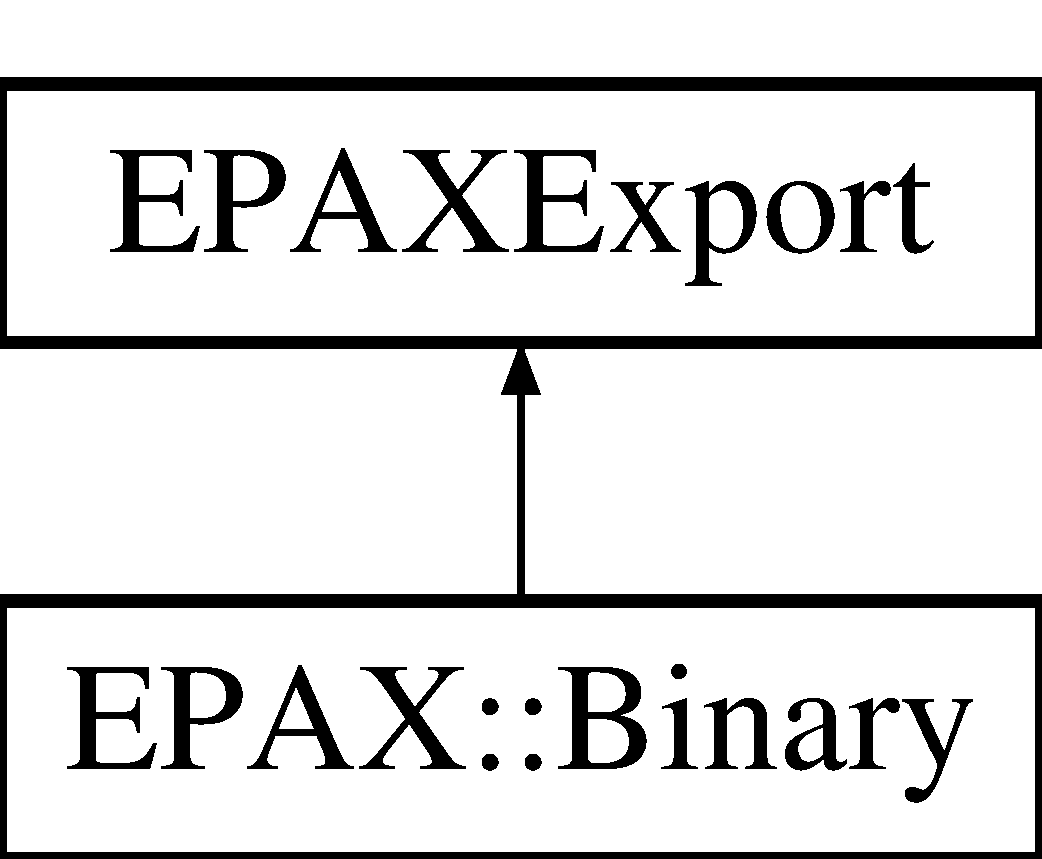
\includegraphics[height=2.000000cm]{class_e_p_a_x_1_1_binary}
\end{center}
\end{figure}
\subsection*{\-Public \-Member \-Functions}
\begin{DoxyCompactItemize}
\item 
\hyperlink{class_e_p_a_x_1_1_binary_ad423337a4b3db46476c82649fc66ecc1}{\-Binary} (std\-::string n)
\item 
\hyperlink{class_e_p_a_x_1_1_binary_ac675512e9efc0881ab5e83a215adfdd6}{\-Binary} (std\-::string n, \hyperlink{namespace_e_p_a_x_a4be639c006ef14def4708b37ee6dd67d}{\-Binary\-Format} f)
\item 
virtual \hyperlink{class_e_p_a_x_1_1_binary_a70f9599a0d1bca21d5754e642047da73}{$\sim$\-Binary} ()
\item 
void \hyperlink{class_e_p_a_x_1_1_binary_a81b916828abd97f8d2e100219f794ca8}{run\-Basic} (int argc, char $\ast$argv\mbox{[}$\,$\mbox{]})
\item 
uint64\-\_\-t \hyperlink{class_e_p_a_x_1_1_binary_a1a0fffa95568cc49ca69d92475866123}{get\-Start\-Addr} ()
\item 
std\-::string \hyperlink{class_e_p_a_x_1_1_binary_a98a84a6650f61a8d991bf9097d9a989b}{get\-Name} ()
\item 
\hyperlink{namespace_e_p_a_x_a4be639c006ef14def4708b37ee6dd67d}{\-Binary\-Format} \hyperlink{class_e_p_a_x_1_1_binary_a77cec506fbd4bc57e5bd0eed0d808902}{get\-Format} ()
\item 
const char $\ast$ \hyperlink{class_e_p_a_x_1_1_binary_aa7cc363e1e514cc97050e85e03c9ed84}{get\-Format\-Name} ()
\item 
uint32\-\_\-t \hyperlink{class_e_p_a_x_1_1_binary_a122d78f5264e90338d9833b181839c95}{count\-Functions} ()
\item 
\hyperlink{class_e_p_a_x_1_1_function}{\-Function} $\ast$ \hyperlink{class_e_p_a_x_1_1_binary_a5616364ee9c96da558b94af2ad299788}{get\-First\-Function} ()
\item 
\hyperlink{class_e_p_a_x_1_1_function}{\-Function} $\ast$ \hyperlink{class_e_p_a_x_1_1_binary_af69f8f6130b81c4c8c09dd380fa62d8d}{get\-Next\-Function} (\hyperlink{class_e_p_a_x_1_1_function}{\-Function} $\ast$f)
\item 
bool \hyperlink{class_e_p_a_x_1_1_binary_a034e51a36f35dd0da6f81d728328e3df}{is\-Last\-Function} (\hyperlink{class_e_p_a_x_1_1_function}{\-Function} $\ast$f)
\item 
\hyperlink{class_e_p_a_x_1_1_function}{\-Function} $\ast$ \hyperlink{class_e_p_a_x_1_1_binary_aed61687c67d986596865c8cd068cfd2f}{find\-Function} (uint64\-\_\-t addr)
\item 
bool \hyperlink{class_e_p_a_x_1_1_binary_a6a4f7d1494137b9f3a3926b620864847}{is\-Executable} ()
\item 
void \hyperlink{class_e_p_a_x_1_1_binary_a05b4aa5fe82b7cc1ef774148f5f57a37}{print\-Static\-File} (std\-::string \&fname)
\item 
void \hyperlink{class_e_p_a_x_1_1_binary_a7d64388704852033519f660d3e5d125f}{print\-Static\-File} (const char $\ast$fname)
\item 
uint32\-\_\-t \hyperlink{class_e_p_a_x_1_1_binary_a875b74e881fb5560eee2bb0e1b8fec43}{get\-File\-Size} ()
\end{DoxyCompactItemize}
\subsection*{\-Static \-Public \-Member \-Functions}
\begin{DoxyCompactItemize}
\item 
static \hyperlink{namespace_e_p_a_x_a4be639c006ef14def4708b37ee6dd67d}{\-Binary\-Format} \hyperlink{class_e_p_a_x_1_1_binary_a915cea1ebad14a5d96f4695f1cc7e1d7}{detect\-Format} (std\-::string n)
\end{DoxyCompactItemize}


\subsection{\-Detailed \-Description}
\-A thin wrapper around the classes which will hold all of the useful information about program binaryies. \-The idea is that this class will provide a single interface on top of any number of different formats. 

\-Definition at line 51 of file \-Binary.\-hpp.



\subsection{\-Constructor \& \-Destructor \-Documentation}
\hypertarget{class_e_p_a_x_1_1_binary_ad423337a4b3db46476c82649fc66ecc1}{\index{\-E\-P\-A\-X\-::\-Binary@{\-E\-P\-A\-X\-::\-Binary}!\-Binary@{\-Binary}}
\index{\-Binary@{\-Binary}!EPAX::Binary@{\-E\-P\-A\-X\-::\-Binary}}
\subsubsection[{\-Binary}]{\setlength{\rightskip}{0pt plus 5cm}{\bf \-E\-P\-A\-X\-::\-Binary\-::\-Binary} (
\begin{DoxyParamCaption}
\item[{std\-::string}]{n}
\end{DoxyParamCaption}
)}}\label{class_e_p_a_x_1_1_binary_ad423337a4b3db46476c82649fc66ecc1}
\-Constructs an \hyperlink{class_e_p_a_x_1_1_binary}{\-Binary} object.


\begin{DoxyParams}{\-Parameters}
{\em n} & \-The name of a file. \-Format will be set based on the file's contents. \\
\hline
\end{DoxyParams}


\-Definition at line 35 of file \-Binary.\-cpp.

\hypertarget{class_e_p_a_x_1_1_binary_ac675512e9efc0881ab5e83a215adfdd6}{\index{\-E\-P\-A\-X\-::\-Binary@{\-E\-P\-A\-X\-::\-Binary}!\-Binary@{\-Binary}}
\index{\-Binary@{\-Binary}!EPAX::Binary@{\-E\-P\-A\-X\-::\-Binary}}
\subsubsection[{\-Binary}]{\setlength{\rightskip}{0pt plus 5cm}{\bf \-E\-P\-A\-X\-::\-Binary\-::\-Binary} (
\begin{DoxyParamCaption}
\item[{std\-::string}]{n, }
\item[{{\bf \-Binary\-Format}}]{f}
\end{DoxyParamCaption}
)}}\label{class_e_p_a_x_1_1_binary_ac675512e9efc0881ab5e83a215adfdd6}
\-Constructs an \hyperlink{class_e_p_a_x_1_1_binary}{\-Binary} object.


\begin{DoxyParams}{\-Parameters}
{\em n} & \-The name of a file. \\
\hline
{\em f} & \-The format of the file. \\
\hline
\end{DoxyParams}


\-Definition at line 41 of file \-Binary.\-cpp.

\hypertarget{class_e_p_a_x_1_1_binary_a70f9599a0d1bca21d5754e642047da73}{\index{\-E\-P\-A\-X\-::\-Binary@{\-E\-P\-A\-X\-::\-Binary}!$\sim$\-Binary@{$\sim$\-Binary}}
\index{$\sim$\-Binary@{$\sim$\-Binary}!EPAX::Binary@{\-E\-P\-A\-X\-::\-Binary}}
\subsubsection[{$\sim$\-Binary}]{\setlength{\rightskip}{0pt plus 5cm}{\bf \-E\-P\-A\-X\-::\-Binary\-::$\sim$\-Binary} (
\begin{DoxyParamCaption}
{}
\end{DoxyParamCaption}
)\hspace{0.3cm}{\ttfamily  \mbox{[}virtual\mbox{]}}}}\label{class_e_p_a_x_1_1_binary_a70f9599a0d1bca21d5754e642047da73}
\-Destroys an \hyperlink{class_e_p_a_x_1_1_binary}{\-Binary} instance. \-Should not be called directly. 

\-Definition at line 47 of file \-Binary.\-cpp.



\subsection{\-Member \-Function \-Documentation}
\hypertarget{class_e_p_a_x_1_1_binary_a122d78f5264e90338d9833b181839c95}{\index{\-E\-P\-A\-X\-::\-Binary@{\-E\-P\-A\-X\-::\-Binary}!count\-Functions@{count\-Functions}}
\index{count\-Functions@{count\-Functions}!EPAX::Binary@{\-E\-P\-A\-X\-::\-Binary}}
\subsubsection[{count\-Functions}]{\setlength{\rightskip}{0pt plus 5cm}uint32\-\_\-t {\bf \-E\-P\-A\-X\-::\-Binary\-::count\-Functions} (
\begin{DoxyParamCaption}
{}
\end{DoxyParamCaption}
)}}\label{class_e_p_a_x_1_1_binary_a122d78f5264e90338d9833b181839c95}
\-Counts the functions in the binary

\begin{DoxyReturn}{\-Returns}
the number of functions in the binary 
\end{DoxyReturn}


\-Definition at line 225 of file \-Binary.\-cpp.

\hypertarget{class_e_p_a_x_1_1_binary_a915cea1ebad14a5d96f4695f1cc7e1d7}{\index{\-E\-P\-A\-X\-::\-Binary@{\-E\-P\-A\-X\-::\-Binary}!detect\-Format@{detect\-Format}}
\index{detect\-Format@{detect\-Format}!EPAX::Binary@{\-E\-P\-A\-X\-::\-Binary}}
\subsubsection[{detect\-Format}]{\setlength{\rightskip}{0pt plus 5cm}{\bf \-Binary\-Format} {\bf \-E\-P\-A\-X\-::\-Binary\-::detect\-Format} (
\begin{DoxyParamCaption}
\item[{std\-::string}]{n}
\end{DoxyParamCaption}
)\hspace{0.3cm}{\ttfamily  \mbox{[}static\mbox{]}}}}\label{class_e_p_a_x_1_1_binary_a915cea1ebad14a5d96f4695f1cc7e1d7}
\-Attempts to guess the format of an binary file

\begin{DoxyReturn}{\-Returns}
the format of the binary file, or \-Binary\-Format\-\_\-undefined(0) if the format cannot be found 
\end{DoxyReturn}


\-Definition at line 160 of file \-Binary.\-cpp.

\hypertarget{class_e_p_a_x_1_1_binary_aed61687c67d986596865c8cd068cfd2f}{\index{\-E\-P\-A\-X\-::\-Binary@{\-E\-P\-A\-X\-::\-Binary}!find\-Function@{find\-Function}}
\index{find\-Function@{find\-Function}!EPAX::Binary@{\-E\-P\-A\-X\-::\-Binary}}
\subsubsection[{find\-Function}]{\setlength{\rightskip}{0pt plus 5cm}{\bf \-Function} $\ast$ {\bf \-E\-P\-A\-X\-::\-Binary\-::find\-Function} (
\begin{DoxyParamCaption}
\item[{uint64\-\_\-t}]{addr}
\end{DoxyParamCaption}
)}}\label{class_e_p_a_x_1_1_binary_aed61687c67d986596865c8cd068cfd2f}


\-Definition at line 221 of file \-Binary.\-cpp.

\hypertarget{class_e_p_a_x_1_1_binary_a875b74e881fb5560eee2bb0e1b8fec43}{\index{\-E\-P\-A\-X\-::\-Binary@{\-E\-P\-A\-X\-::\-Binary}!get\-File\-Size@{get\-File\-Size}}
\index{get\-File\-Size@{get\-File\-Size}!EPAX::Binary@{\-E\-P\-A\-X\-::\-Binary}}
\subsubsection[{get\-File\-Size}]{\setlength{\rightskip}{0pt plus 5cm}uint32\-\_\-t {\bf \-E\-P\-A\-X\-::\-Binary\-::get\-File\-Size} (
\begin{DoxyParamCaption}
{}
\end{DoxyParamCaption}
)}}\label{class_e_p_a_x_1_1_binary_a875b74e881fb5560eee2bb0e1b8fec43}


\-Definition at line 233 of file \-Binary.\-cpp.

\hypertarget{class_e_p_a_x_1_1_binary_a5616364ee9c96da558b94af2ad299788}{\index{\-E\-P\-A\-X\-::\-Binary@{\-E\-P\-A\-X\-::\-Binary}!get\-First\-Function@{get\-First\-Function}}
\index{get\-First\-Function@{get\-First\-Function}!EPAX::Binary@{\-E\-P\-A\-X\-::\-Binary}}
\subsubsection[{get\-First\-Function}]{\setlength{\rightskip}{0pt plus 5cm}{\bf \-Function} $\ast$ {\bf \-E\-P\-A\-X\-::\-Binary\-::get\-First\-Function} (
\begin{DoxyParamCaption}
{}
\end{DoxyParamCaption}
)}}\label{class_e_p_a_x_1_1_binary_a5616364ee9c96da558b94af2ad299788}
\-Gets the first function in the binary

\begin{DoxyReturn}{\-Returns}
the first function in the binary 
\end{DoxyReturn}


\-Definition at line 209 of file \-Binary.\-cpp.

\hypertarget{class_e_p_a_x_1_1_binary_a77cec506fbd4bc57e5bd0eed0d808902}{\index{\-E\-P\-A\-X\-::\-Binary@{\-E\-P\-A\-X\-::\-Binary}!get\-Format@{get\-Format}}
\index{get\-Format@{get\-Format}!EPAX::Binary@{\-E\-P\-A\-X\-::\-Binary}}
\subsubsection[{get\-Format}]{\setlength{\rightskip}{0pt plus 5cm}{\bf \-Binary\-Format} {\bf \-E\-P\-A\-X\-::\-Binary\-::get\-Format} (
\begin{DoxyParamCaption}
{}
\end{DoxyParamCaption}
)\hspace{0.3cm}{\ttfamily  \mbox{[}inline\mbox{]}}}}\label{class_e_p_a_x_1_1_binary_a77cec506fbd4bc57e5bd0eed0d808902}
\-Gets the format of the binary.

\begin{DoxyReturn}{\-Returns}
the format of this binary 
\end{DoxyReturn}


\-Definition at line 106 of file \-Binary.\-hpp.

\hypertarget{class_e_p_a_x_1_1_binary_aa7cc363e1e514cc97050e85e03c9ed84}{\index{\-E\-P\-A\-X\-::\-Binary@{\-E\-P\-A\-X\-::\-Binary}!get\-Format\-Name@{get\-Format\-Name}}
\index{get\-Format\-Name@{get\-Format\-Name}!EPAX::Binary@{\-E\-P\-A\-X\-::\-Binary}}
\subsubsection[{get\-Format\-Name}]{\setlength{\rightskip}{0pt plus 5cm}const char $\ast$ {\bf \-E\-P\-A\-X\-::\-Binary\-::get\-Format\-Name} (
\begin{DoxyParamCaption}
{}
\end{DoxyParamCaption}
)}}\label{class_e_p_a_x_1_1_binary_aa7cc363e1e514cc97050e85e03c9ed84}
\-Gets a string representation of the format of this binary.

@ return a string representation of the format of this binary 

\-Definition at line 123 of file \-Binary.\-cpp.

\hypertarget{class_e_p_a_x_1_1_binary_a98a84a6650f61a8d991bf9097d9a989b}{\index{\-E\-P\-A\-X\-::\-Binary@{\-E\-P\-A\-X\-::\-Binary}!get\-Name@{get\-Name}}
\index{get\-Name@{get\-Name}!EPAX::Binary@{\-E\-P\-A\-X\-::\-Binary}}
\subsubsection[{get\-Name}]{\setlength{\rightskip}{0pt plus 5cm}std\-::string {\bf \-E\-P\-A\-X\-::\-Binary\-::get\-Name} (
\begin{DoxyParamCaption}
{}
\end{DoxyParamCaption}
)}}\label{class_e_p_a_x_1_1_binary_a98a84a6650f61a8d991bf9097d9a989b}


\-Definition at line 205 of file \-Binary.\-cpp.

\hypertarget{class_e_p_a_x_1_1_binary_af69f8f6130b81c4c8c09dd380fa62d8d}{\index{\-E\-P\-A\-X\-::\-Binary@{\-E\-P\-A\-X\-::\-Binary}!get\-Next\-Function@{get\-Next\-Function}}
\index{get\-Next\-Function@{get\-Next\-Function}!EPAX::Binary@{\-E\-P\-A\-X\-::\-Binary}}
\subsubsection[{get\-Next\-Function}]{\setlength{\rightskip}{0pt plus 5cm}{\bf \-Function} $\ast$ {\bf \-E\-P\-A\-X\-::\-Binary\-::get\-Next\-Function} (
\begin{DoxyParamCaption}
\item[{{\bf \-Function} $\ast$}]{f}
\end{DoxyParamCaption}
)}}\label{class_e_p_a_x_1_1_binary_af69f8f6130b81c4c8c09dd380fa62d8d}
\-Gets the next function in the binary


\begin{DoxyParams}{\-Parameters}
{\em f} & a function in the binary\\
\hline
\end{DoxyParams}
\begin{DoxyReturn}{\-Returns}
the function following f 
\end{DoxyReturn}


\-Definition at line 213 of file \-Binary.\-cpp.

\hypertarget{class_e_p_a_x_1_1_binary_a1a0fffa95568cc49ca69d92475866123}{\index{\-E\-P\-A\-X\-::\-Binary@{\-E\-P\-A\-X\-::\-Binary}!get\-Start\-Addr@{get\-Start\-Addr}}
\index{get\-Start\-Addr@{get\-Start\-Addr}!EPAX::Binary@{\-E\-P\-A\-X\-::\-Binary}}
\subsubsection[{get\-Start\-Addr}]{\setlength{\rightskip}{0pt plus 5cm}uint64\-\_\-t {\bf \-E\-P\-A\-X\-::\-Binary\-::get\-Start\-Addr} (
\begin{DoxyParamCaption}
{}
\end{DoxyParamCaption}
)}}\label{class_e_p_a_x_1_1_binary_a1a0fffa95568cc49ca69d92475866123}


\-Definition at line 201 of file \-Binary.\-cpp.

\hypertarget{class_e_p_a_x_1_1_binary_a6a4f7d1494137b9f3a3926b620864847}{\index{\-E\-P\-A\-X\-::\-Binary@{\-E\-P\-A\-X\-::\-Binary}!is\-Executable@{is\-Executable}}
\index{is\-Executable@{is\-Executable}!EPAX::Binary@{\-E\-P\-A\-X\-::\-Binary}}
\subsubsection[{is\-Executable}]{\setlength{\rightskip}{0pt plus 5cm}bool {\bf \-E\-P\-A\-X\-::\-Binary\-::is\-Executable} (
\begin{DoxyParamCaption}
{}
\end{DoxyParamCaption}
)}}\label{class_e_p_a_x_1_1_binary_a6a4f7d1494137b9f3a3926b620864847}


\-Definition at line 229 of file \-Binary.\-cpp.

\hypertarget{class_e_p_a_x_1_1_binary_a034e51a36f35dd0da6f81d728328e3df}{\index{\-E\-P\-A\-X\-::\-Binary@{\-E\-P\-A\-X\-::\-Binary}!is\-Last\-Function@{is\-Last\-Function}}
\index{is\-Last\-Function@{is\-Last\-Function}!EPAX::Binary@{\-E\-P\-A\-X\-::\-Binary}}
\subsubsection[{is\-Last\-Function}]{\setlength{\rightskip}{0pt plus 5cm}bool {\bf \-E\-P\-A\-X\-::\-Binary\-::is\-Last\-Function} (
\begin{DoxyParamCaption}
\item[{{\bf \-Function} $\ast$}]{f}
\end{DoxyParamCaption}
)}}\label{class_e_p_a_x_1_1_binary_a034e51a36f35dd0da6f81d728328e3df}
\-Tells whether this is the last function in the binary


\begin{DoxyParams}{\-Parameters}
{\em f} & a function in the binary\\
\hline
\end{DoxyParams}
\begin{DoxyReturn}{\-Returns}
true iff f is the last function in the binary 
\end{DoxyReturn}


\-Definition at line 217 of file \-Binary.\-cpp.

\hypertarget{class_e_p_a_x_1_1_binary_a05b4aa5fe82b7cc1ef774148f5f57a37}{\index{\-E\-P\-A\-X\-::\-Binary@{\-E\-P\-A\-X\-::\-Binary}!print\-Static\-File@{print\-Static\-File}}
\index{print\-Static\-File@{print\-Static\-File}!EPAX::Binary@{\-E\-P\-A\-X\-::\-Binary}}
\subsubsection[{print\-Static\-File}]{\setlength{\rightskip}{0pt plus 5cm}void {\bf \-E\-P\-A\-X\-::\-Binary\-::print\-Static\-File} (
\begin{DoxyParamCaption}
\item[{std\-::string \&}]{fname}
\end{DoxyParamCaption}
)}}\label{class_e_p_a_x_1_1_binary_a05b4aa5fe82b7cc1ef774148f5f57a37}


\-Definition at line 53 of file \-Binary.\-cpp.

\hypertarget{class_e_p_a_x_1_1_binary_a7d64388704852033519f660d3e5d125f}{\index{\-E\-P\-A\-X\-::\-Binary@{\-E\-P\-A\-X\-::\-Binary}!print\-Static\-File@{print\-Static\-File}}
\index{print\-Static\-File@{print\-Static\-File}!EPAX::Binary@{\-E\-P\-A\-X\-::\-Binary}}
\subsubsection[{print\-Static\-File}]{\setlength{\rightskip}{0pt plus 5cm}void {\bf \-E\-P\-A\-X\-::\-Binary\-::print\-Static\-File} (
\begin{DoxyParamCaption}
\item[{const char $\ast$}]{fname}
\end{DoxyParamCaption}
)}}\label{class_e_p_a_x_1_1_binary_a7d64388704852033519f660d3e5d125f}


\-Definition at line 57 of file \-Binary.\-cpp.

\hypertarget{class_e_p_a_x_1_1_binary_a81b916828abd97f8d2e100219f794ca8}{\index{\-E\-P\-A\-X\-::\-Binary@{\-E\-P\-A\-X\-::\-Binary}!run\-Basic@{run\-Basic}}
\index{run\-Basic@{run\-Basic}!EPAX::Binary@{\-E\-P\-A\-X\-::\-Binary}}
\subsubsection[{run\-Basic}]{\setlength{\rightskip}{0pt plus 5cm}void {\bf \-E\-P\-A\-X\-::\-Binary\-::run\-Basic} (
\begin{DoxyParamCaption}
\item[{int}]{argc, }
\item[{char $\ast$}]{argv\mbox{[}$\,$\mbox{]}}
\end{DoxyParamCaption}
)}}\label{class_e_p_a_x_1_1_binary_a81b916828abd97f8d2e100219f794ca8}


\-Definition at line 69 of file \-Binary.\-cpp.



\-The documentation for this class was generated from the following files\-:\begin{DoxyCompactItemize}
\item 
\hyperlink{_binary_8hpp}{\-Binary.\-hpp}\item 
\hyperlink{_binary_8cpp}{\-Binary.\-cpp}\end{DoxyCompactItemize}

\hypertarget{class_e_p_a_x_1_1_control_flow}{\section{\-E\-P\-A\-X\-:\-:\-Control\-Flow \-Class \-Reference}
\label{class_e_p_a_x_1_1_control_flow}\index{\-E\-P\-A\-X\-::\-Control\-Flow@{\-E\-P\-A\-X\-::\-Control\-Flow}}
}


{\ttfamily \#include $<$\-Control\-Flow.\-hpp$>$}

\-Inheritance diagram for \-E\-P\-A\-X\-:\-:\-Control\-Flow\-:\begin{figure}[H]
\begin{center}
\leavevmode
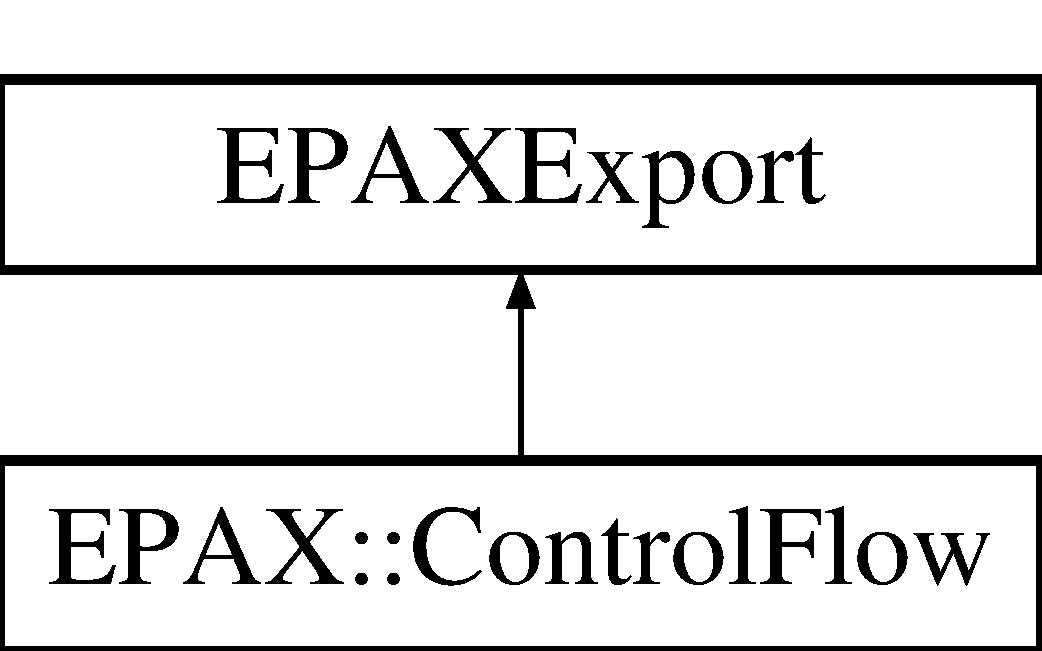
\includegraphics[height=2.000000cm]{class_e_p_a_x_1_1_control_flow}
\end{center}
\end{figure}
\subsection*{\-Public \-Member \-Functions}
\begin{DoxyCompactItemize}
\item 
\hyperlink{class_e_p_a_x_1_1_control_flow_aae2b7a80785816f4edc564f740e575c7}{\-Control\-Flow} (\hyperlink{class_e_p_a_x_1_1_function}{\-Function} $\ast$f, std\-::vector$<$ \hyperlink{class_e_p_a_x_1_1_basic_block}{\-Basic\-Block} $\ast$ $>$ bbs)
\item 
virtual \hyperlink{class_e_p_a_x_1_1_control_flow_a8823aec1b9b95147997176c3d649961f}{$\sim$\-Control\-Flow} ()
\item 
\hyperlink{class_e_p_a_x_1_1_function}{\-Function} $\ast$ \hyperlink{class_e_p_a_x_1_1_control_flow_ae8d9d902fd8c7d55d3a8492b9221ca90}{get\-Function} ()
\item 
void \hyperlink{class_e_p_a_x_1_1_control_flow_a5946e49014e4f689b6e9ec1f4d40d574}{print} (std\-::ostream \&stream=std\-::cout)
\item 
void \hyperlink{class_e_p_a_x_1_1_control_flow_a63fa0089dbc656ac9b862f6ac7e6f97a}{dot\-\_\-print} (std\-::ostream \&stream=std\-::cout)
\item 
uint32\-\_\-t \hyperlink{class_e_p_a_x_1_1_control_flow_a9c9e7392073a46b804756be6ad9e3b20}{count\-Basic\-Blocks} ()
\item 
\hyperlink{class_e_p_a_x_1_1_basic_block}{\-Basic\-Block} $\ast$ \hyperlink{class_e_p_a_x_1_1_control_flow_ae7c4d1a074d965533fd4b41acadf183e}{find\-Basic\-Block} (uint64\-\_\-t addr)
\item 
\hyperlink{class_e_p_a_x_1_1_basic_block}{\-Basic\-Block} $\ast$ \hyperlink{class_e_p_a_x_1_1_control_flow_ac0dfd67d0514dc086a13ba3969d8ae71}{get\-Basic\-Block} (uint32\-\_\-t idx)
\item 
uint32\-\_\-t \hyperlink{class_e_p_a_x_1_1_control_flow_ad68be1fbfb8a262bfb4812e1ccc769d8}{count\-Instructions} ()
\item 
\hyperlink{class_e_p_a_x_1_1_instruction}{\-Instruction} $\ast$ \hyperlink{class_e_p_a_x_1_1_control_flow_a4340905b7507964731967fd00ca5ce6f}{find\-Instruction} (uint64\-\_\-t addr)
\item 
\hyperlink{class_e_p_a_x_1_1_instruction}{\-Instruction} $\ast$ \hyperlink{class_e_p_a_x_1_1_control_flow_acdd2cfc96f19c5d0aa6ef884b0379808}{get\-Instruction} (uint32\-\_\-t idx)
\item 
uint32\-\_\-t \hyperlink{class_e_p_a_x_1_1_control_flow_aac44b527eddbacb18362a17efa5a3627}{count\-Loops} ()
\item 
\hyperlink{class_e_p_a_x_1_1_loop}{\-Loop} $\ast$ \hyperlink{class_e_p_a_x_1_1_control_flow_a21c1c89f5abaca190a3001e78fc0f4de}{find\-Loop} (uint64\-\_\-t addr)
\item 
\hyperlink{class_e_p_a_x_1_1_loop}{\-Loop} $\ast$ \hyperlink{class_e_p_a_x_1_1_control_flow_a71b3bbea4d16dc52483c53db0e87b365}{get\-Loop} (uint32\-\_\-t idx)
\item 
\hyperlink{class_e_p_a_x_1_1_loop}{\-Loop} $\ast$ \hyperlink{class_e_p_a_x_1_1_control_flow_aba17ac8471189701a17143e272360f1b}{get\-Parent\-Of} (\hyperlink{class_e_p_a_x_1_1_loop}{\-Loop} $\ast$loop)
\end{DoxyCompactItemize}


\subsection{\-Detailed \-Description}


\-Definition at line 37 of file \-Control\-Flow.\-hpp.



\subsection{\-Constructor \& \-Destructor \-Documentation}
\hypertarget{class_e_p_a_x_1_1_control_flow_aae2b7a80785816f4edc564f740e575c7}{\index{\-E\-P\-A\-X\-::\-Control\-Flow@{\-E\-P\-A\-X\-::\-Control\-Flow}!\-Control\-Flow@{\-Control\-Flow}}
\index{\-Control\-Flow@{\-Control\-Flow}!EPAX::ControlFlow@{\-E\-P\-A\-X\-::\-Control\-Flow}}
\subsubsection[{\-Control\-Flow}]{\setlength{\rightskip}{0pt plus 5cm}{\bf \-E\-P\-A\-X\-::\-Control\-Flow\-::\-Control\-Flow} (
\begin{DoxyParamCaption}
\item[{{\bf \-Function} $\ast$}]{f, }
\item[{std\-::vector$<$ {\bf \-Basic\-Block} $\ast$ $>$}]{bbs}
\end{DoxyParamCaption}
)}}\label{class_e_p_a_x_1_1_control_flow_aae2b7a80785816f4edc564f740e575c7}


\-Definition at line 35 of file \-Control\-Flow.\-cpp.

\hypertarget{class_e_p_a_x_1_1_control_flow_a8823aec1b9b95147997176c3d649961f}{\index{\-E\-P\-A\-X\-::\-Control\-Flow@{\-E\-P\-A\-X\-::\-Control\-Flow}!$\sim$\-Control\-Flow@{$\sim$\-Control\-Flow}}
\index{$\sim$\-Control\-Flow@{$\sim$\-Control\-Flow}!EPAX::ControlFlow@{\-E\-P\-A\-X\-::\-Control\-Flow}}
\subsubsection[{$\sim$\-Control\-Flow}]{\setlength{\rightskip}{0pt plus 5cm}{\bf \-E\-P\-A\-X\-::\-Control\-Flow\-::$\sim$\-Control\-Flow} (
\begin{DoxyParamCaption}
{}
\end{DoxyParamCaption}
)\hspace{0.3cm}{\ttfamily  \mbox{[}virtual\mbox{]}}}}\label{class_e_p_a_x_1_1_control_flow_a8823aec1b9b95147997176c3d649961f}


\-Definition at line 42 of file \-Control\-Flow.\-cpp.



\subsection{\-Member \-Function \-Documentation}
\hypertarget{class_e_p_a_x_1_1_control_flow_a9c9e7392073a46b804756be6ad9e3b20}{\index{\-E\-P\-A\-X\-::\-Control\-Flow@{\-E\-P\-A\-X\-::\-Control\-Flow}!count\-Basic\-Blocks@{count\-Basic\-Blocks}}
\index{count\-Basic\-Blocks@{count\-Basic\-Blocks}!EPAX::ControlFlow@{\-E\-P\-A\-X\-::\-Control\-Flow}}
\subsubsection[{count\-Basic\-Blocks}]{\setlength{\rightskip}{0pt plus 5cm}uint32\-\_\-t {\bf \-E\-P\-A\-X\-::\-Control\-Flow\-::count\-Basic\-Blocks} (
\begin{DoxyParamCaption}
{}
\end{DoxyParamCaption}
)}}\label{class_e_p_a_x_1_1_control_flow_a9c9e7392073a46b804756be6ad9e3b20}


\-Definition at line 300 of file \-Control\-Flow.\-cpp.

\hypertarget{class_e_p_a_x_1_1_control_flow_ad68be1fbfb8a262bfb4812e1ccc769d8}{\index{\-E\-P\-A\-X\-::\-Control\-Flow@{\-E\-P\-A\-X\-::\-Control\-Flow}!count\-Instructions@{count\-Instructions}}
\index{count\-Instructions@{count\-Instructions}!EPAX::ControlFlow@{\-E\-P\-A\-X\-::\-Control\-Flow}}
\subsubsection[{count\-Instructions}]{\setlength{\rightskip}{0pt plus 5cm}uint32\-\_\-t {\bf \-E\-P\-A\-X\-::\-Control\-Flow\-::count\-Instructions} (
\begin{DoxyParamCaption}
{}
\end{DoxyParamCaption}
)}}\label{class_e_p_a_x_1_1_control_flow_ad68be1fbfb8a262bfb4812e1ccc769d8}


\-Definition at line 322 of file \-Control\-Flow.\-cpp.

\hypertarget{class_e_p_a_x_1_1_control_flow_aac44b527eddbacb18362a17efa5a3627}{\index{\-E\-P\-A\-X\-::\-Control\-Flow@{\-E\-P\-A\-X\-::\-Control\-Flow}!count\-Loops@{count\-Loops}}
\index{count\-Loops@{count\-Loops}!EPAX::ControlFlow@{\-E\-P\-A\-X\-::\-Control\-Flow}}
\subsubsection[{count\-Loops}]{\setlength{\rightskip}{0pt plus 5cm}uint32\-\_\-t {\bf \-E\-P\-A\-X\-::\-Control\-Flow\-::count\-Loops} (
\begin{DoxyParamCaption}
{}
\end{DoxyParamCaption}
)}}\label{class_e_p_a_x_1_1_control_flow_aac44b527eddbacb18362a17efa5a3627}


\-Definition at line 344 of file \-Control\-Flow.\-cpp.

\hypertarget{class_e_p_a_x_1_1_control_flow_a63fa0089dbc656ac9b862f6ac7e6f97a}{\index{\-E\-P\-A\-X\-::\-Control\-Flow@{\-E\-P\-A\-X\-::\-Control\-Flow}!dot\-\_\-print@{dot\-\_\-print}}
\index{dot\-\_\-print@{dot\-\_\-print}!EPAX::ControlFlow@{\-E\-P\-A\-X\-::\-Control\-Flow}}
\subsubsection[{dot\-\_\-print}]{\setlength{\rightskip}{0pt plus 5cm}void {\bf \-E\-P\-A\-X\-::\-Control\-Flow\-::dot\-\_\-print} (
\begin{DoxyParamCaption}
\item[{std\-::ostream \&}]{stream = {\ttfamily std\-:\-:cout}}
\end{DoxyParamCaption}
)}}\label{class_e_p_a_x_1_1_control_flow_a63fa0089dbc656ac9b862f6ac7e6f97a}


\-Definition at line 275 of file \-Control\-Flow.\-cpp.

\hypertarget{class_e_p_a_x_1_1_control_flow_ae7c4d1a074d965533fd4b41acadf183e}{\index{\-E\-P\-A\-X\-::\-Control\-Flow@{\-E\-P\-A\-X\-::\-Control\-Flow}!find\-Basic\-Block@{find\-Basic\-Block}}
\index{find\-Basic\-Block@{find\-Basic\-Block}!EPAX::ControlFlow@{\-E\-P\-A\-X\-::\-Control\-Flow}}
\subsubsection[{find\-Basic\-Block}]{\setlength{\rightskip}{0pt plus 5cm}{\bf \-Basic\-Block} $\ast$ {\bf \-E\-P\-A\-X\-::\-Control\-Flow\-::find\-Basic\-Block} (
\begin{DoxyParamCaption}
\item[{uint64\-\_\-t}]{addr}
\end{DoxyParamCaption}
)}}\label{class_e_p_a_x_1_1_control_flow_ae7c4d1a074d965533fd4b41acadf183e}


\-Definition at line 304 of file \-Control\-Flow.\-cpp.

\hypertarget{class_e_p_a_x_1_1_control_flow_a4340905b7507964731967fd00ca5ce6f}{\index{\-E\-P\-A\-X\-::\-Control\-Flow@{\-E\-P\-A\-X\-::\-Control\-Flow}!find\-Instruction@{find\-Instruction}}
\index{find\-Instruction@{find\-Instruction}!EPAX::ControlFlow@{\-E\-P\-A\-X\-::\-Control\-Flow}}
\subsubsection[{find\-Instruction}]{\setlength{\rightskip}{0pt plus 5cm}{\bf \-Instruction} $\ast$ {\bf \-E\-P\-A\-X\-::\-Control\-Flow\-::find\-Instruction} (
\begin{DoxyParamCaption}
\item[{uint64\-\_\-t}]{addr}
\end{DoxyParamCaption}
)}}\label{class_e_p_a_x_1_1_control_flow_a4340905b7507964731967fd00ca5ce6f}


\-Definition at line 326 of file \-Control\-Flow.\-cpp.

\hypertarget{class_e_p_a_x_1_1_control_flow_a21c1c89f5abaca190a3001e78fc0f4de}{\index{\-E\-P\-A\-X\-::\-Control\-Flow@{\-E\-P\-A\-X\-::\-Control\-Flow}!find\-Loop@{find\-Loop}}
\index{find\-Loop@{find\-Loop}!EPAX::ControlFlow@{\-E\-P\-A\-X\-::\-Control\-Flow}}
\subsubsection[{find\-Loop}]{\setlength{\rightskip}{0pt plus 5cm}{\bf \-Loop} $\ast$ {\bf \-E\-P\-A\-X\-::\-Control\-Flow\-::find\-Loop} (
\begin{DoxyParamCaption}
\item[{uint64\-\_\-t}]{addr}
\end{DoxyParamCaption}
)}}\label{class_e_p_a_x_1_1_control_flow_a21c1c89f5abaca190a3001e78fc0f4de}


\-Definition at line 348 of file \-Control\-Flow.\-cpp.

\hypertarget{class_e_p_a_x_1_1_control_flow_ac0dfd67d0514dc086a13ba3969d8ae71}{\index{\-E\-P\-A\-X\-::\-Control\-Flow@{\-E\-P\-A\-X\-::\-Control\-Flow}!get\-Basic\-Block@{get\-Basic\-Block}}
\index{get\-Basic\-Block@{get\-Basic\-Block}!EPAX::ControlFlow@{\-E\-P\-A\-X\-::\-Control\-Flow}}
\subsubsection[{get\-Basic\-Block}]{\setlength{\rightskip}{0pt plus 5cm}{\bf \-Basic\-Block} $\ast$ {\bf \-E\-P\-A\-X\-::\-Control\-Flow\-::get\-Basic\-Block} (
\begin{DoxyParamCaption}
\item[{uint32\-\_\-t}]{idx}
\end{DoxyParamCaption}
)}}\label{class_e_p_a_x_1_1_control_flow_ac0dfd67d0514dc086a13ba3969d8ae71}


\-Definition at line 315 of file \-Control\-Flow.\-cpp.

\hypertarget{class_e_p_a_x_1_1_control_flow_ae8d9d902fd8c7d55d3a8492b9221ca90}{\index{\-E\-P\-A\-X\-::\-Control\-Flow@{\-E\-P\-A\-X\-::\-Control\-Flow}!get\-Function@{get\-Function}}
\index{get\-Function@{get\-Function}!EPAX::ControlFlow@{\-E\-P\-A\-X\-::\-Control\-Flow}}
\subsubsection[{get\-Function}]{\setlength{\rightskip}{0pt plus 5cm}{\bf \-Function}$\ast$ {\bf \-E\-P\-A\-X\-::\-Control\-Flow\-::get\-Function} (
\begin{DoxyParamCaption}
{}
\end{DoxyParamCaption}
)\hspace{0.3cm}{\ttfamily  \mbox{[}inline\mbox{]}}}}\label{class_e_p_a_x_1_1_control_flow_ae8d9d902fd8c7d55d3a8492b9221ca90}


\-Definition at line 52 of file \-Control\-Flow.\-hpp.

\hypertarget{class_e_p_a_x_1_1_control_flow_acdd2cfc96f19c5d0aa6ef884b0379808}{\index{\-E\-P\-A\-X\-::\-Control\-Flow@{\-E\-P\-A\-X\-::\-Control\-Flow}!get\-Instruction@{get\-Instruction}}
\index{get\-Instruction@{get\-Instruction}!EPAX::ControlFlow@{\-E\-P\-A\-X\-::\-Control\-Flow}}
\subsubsection[{get\-Instruction}]{\setlength{\rightskip}{0pt plus 5cm}{\bf \-Instruction} $\ast$ {\bf \-E\-P\-A\-X\-::\-Control\-Flow\-::get\-Instruction} (
\begin{DoxyParamCaption}
\item[{uint32\-\_\-t}]{idx}
\end{DoxyParamCaption}
)}}\label{class_e_p_a_x_1_1_control_flow_acdd2cfc96f19c5d0aa6ef884b0379808}


\-Definition at line 337 of file \-Control\-Flow.\-cpp.

\hypertarget{class_e_p_a_x_1_1_control_flow_a71b3bbea4d16dc52483c53db0e87b365}{\index{\-E\-P\-A\-X\-::\-Control\-Flow@{\-E\-P\-A\-X\-::\-Control\-Flow}!get\-Loop@{get\-Loop}}
\index{get\-Loop@{get\-Loop}!EPAX::ControlFlow@{\-E\-P\-A\-X\-::\-Control\-Flow}}
\subsubsection[{get\-Loop}]{\setlength{\rightskip}{0pt plus 5cm}{\bf \-Loop} $\ast$ {\bf \-E\-P\-A\-X\-::\-Control\-Flow\-::get\-Loop} (
\begin{DoxyParamCaption}
\item[{uint32\-\_\-t}]{idx}
\end{DoxyParamCaption}
)}}\label{class_e_p_a_x_1_1_control_flow_a71b3bbea4d16dc52483c53db0e87b365}


\-Definition at line 368 of file \-Control\-Flow.\-cpp.

\hypertarget{class_e_p_a_x_1_1_control_flow_aba17ac8471189701a17143e272360f1b}{\index{\-E\-P\-A\-X\-::\-Control\-Flow@{\-E\-P\-A\-X\-::\-Control\-Flow}!get\-Parent\-Of@{get\-Parent\-Of}}
\index{get\-Parent\-Of@{get\-Parent\-Of}!EPAX::ControlFlow@{\-E\-P\-A\-X\-::\-Control\-Flow}}
\subsubsection[{get\-Parent\-Of}]{\setlength{\rightskip}{0pt plus 5cm}{\bf \-Loop} $\ast$ {\bf \-E\-P\-A\-X\-::\-Control\-Flow\-::get\-Parent\-Of} (
\begin{DoxyParamCaption}
\item[{{\bf \-Loop} $\ast$}]{loop}
\end{DoxyParamCaption}
)}}\label{class_e_p_a_x_1_1_control_flow_aba17ac8471189701a17143e272360f1b}


\-Definition at line 291 of file \-Control\-Flow.\-cpp.

\hypertarget{class_e_p_a_x_1_1_control_flow_a5946e49014e4f689b6e9ec1f4d40d574}{\index{\-E\-P\-A\-X\-::\-Control\-Flow@{\-E\-P\-A\-X\-::\-Control\-Flow}!print@{print}}
\index{print@{print}!EPAX::ControlFlow@{\-E\-P\-A\-X\-::\-Control\-Flow}}
\subsubsection[{print}]{\setlength{\rightskip}{0pt plus 5cm}void {\bf \-E\-P\-A\-X\-::\-Control\-Flow\-::print} (
\begin{DoxyParamCaption}
\item[{std\-::ostream \&}]{stream = {\ttfamily std\-:\-:cout}}
\end{DoxyParamCaption}
)}}\label{class_e_p_a_x_1_1_control_flow_a5946e49014e4f689b6e9ec1f4d40d574}


\-Definition at line 267 of file \-Control\-Flow.\-cpp.



\-The documentation for this class was generated from the following files\-:\begin{DoxyCompactItemize}
\item 
\hyperlink{_control_flow_8hpp}{\-Control\-Flow.\-hpp}\item 
\hyperlink{_control_flow_8cpp}{\-Control\-Flow.\-cpp}\end{DoxyCompactItemize}

\hypertarget{class_e_p_a_x_1_1_detached_text}{\section{\-E\-P\-A\-X\-:\-:\-Detached\-Text \-Class \-Reference}
\label{class_e_p_a_x_1_1_detached_text}\index{\-E\-P\-A\-X\-::\-Detached\-Text@{\-E\-P\-A\-X\-::\-Detached\-Text}}
}


{\ttfamily \#include $<$\-Function.\-hpp$>$}

\-Inheritance diagram for \-E\-P\-A\-X\-:\-:\-Detached\-Text\-:\begin{figure}[H]
\begin{center}
\leavevmode
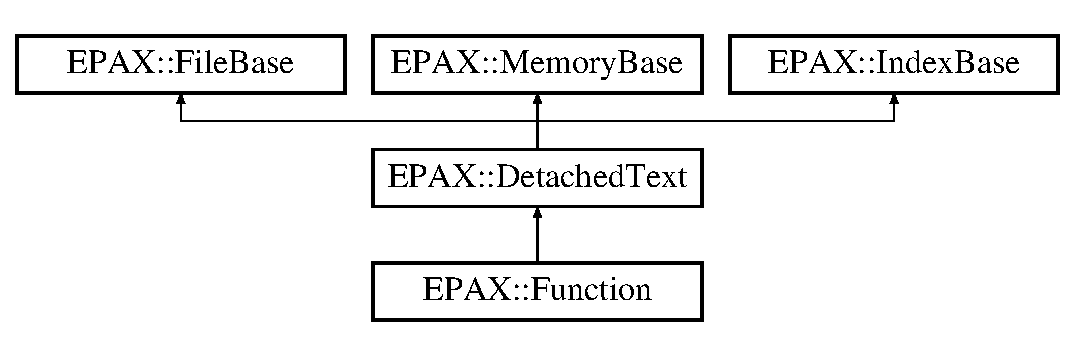
\includegraphics[height=3.000000cm]{class_e_p_a_x_1_1_detached_text}
\end{center}
\end{figure}
\subsection*{\-Public \-Member \-Functions}
\begin{DoxyCompactItemize}
\item 
\hyperlink{class_e_p_a_x_1_1_detached_text_ae79447b52406259983750894d291dcef}{\-Detached\-Text} (\hyperlink{class_e_p_a_x_1_1_base_binary}{\-Base\-Binary} $\ast$b, uint64\-\_\-t o, uint64\-\_\-t s, uint64\-\_\-t a, uint32\-\_\-t i)
\item 
virtual \hyperlink{class_e_p_a_x_1_1_detached_text_ac55a477e1fbdb7ed76f148c56fd782df}{$\sim$\-Detached\-Text} ()
\item 
virtual void \hyperlink{class_e_p_a_x_1_1_detached_text_a8a32ccd60ccd9a710a84301b4c483902}{print} (std\-::ostream \&stream=std\-::cout)
\end{DoxyCompactItemize}
\subsection*{\-Protected \-Attributes}
\begin{DoxyCompactItemize}
\item 
std\-::vector$<$ void $\ast$ $>$ \hyperlink{class_e_p_a_x_1_1_detached_text_afd3624b03921f90ff4c2cd2a1d172e76}{instructions}
\end{DoxyCompactItemize}


\subsection{\-Detailed \-Description}


\-Definition at line 43 of file \-Function.\-hpp.



\subsection{\-Constructor \& \-Destructor \-Documentation}
\hypertarget{class_e_p_a_x_1_1_detached_text_ae79447b52406259983750894d291dcef}{\index{\-E\-P\-A\-X\-::\-Detached\-Text@{\-E\-P\-A\-X\-::\-Detached\-Text}!\-Detached\-Text@{\-Detached\-Text}}
\index{\-Detached\-Text@{\-Detached\-Text}!EPAX::DetachedText@{\-E\-P\-A\-X\-::\-Detached\-Text}}
\subsubsection[{\-Detached\-Text}]{\setlength{\rightskip}{0pt plus 5cm}{\bf \-E\-P\-A\-X\-::\-Detached\-Text\-::\-Detached\-Text} (
\begin{DoxyParamCaption}
\item[{{\bf \-Base\-Binary} $\ast$}]{b, }
\item[{uint64\-\_\-t}]{o, }
\item[{uint64\-\_\-t}]{s, }
\item[{uint64\-\_\-t}]{a, }
\item[{uint32\-\_\-t}]{i}
\end{DoxyParamCaption}
)}}\label{class_e_p_a_x_1_1_detached_text_ae79447b52406259983750894d291dcef}


\-Definition at line 36 of file \-Function.\-cpp.

\hypertarget{class_e_p_a_x_1_1_detached_text_ac55a477e1fbdb7ed76f148c56fd782df}{\index{\-E\-P\-A\-X\-::\-Detached\-Text@{\-E\-P\-A\-X\-::\-Detached\-Text}!$\sim$\-Detached\-Text@{$\sim$\-Detached\-Text}}
\index{$\sim$\-Detached\-Text@{$\sim$\-Detached\-Text}!EPAX::DetachedText@{\-E\-P\-A\-X\-::\-Detached\-Text}}
\subsubsection[{$\sim$\-Detached\-Text}]{\setlength{\rightskip}{0pt plus 5cm}virtual {\bf \-E\-P\-A\-X\-::\-Detached\-Text\-::$\sim$\-Detached\-Text} (
\begin{DoxyParamCaption}
{}
\end{DoxyParamCaption}
)\hspace{0.3cm}{\ttfamily  \mbox{[}inline, virtual\mbox{]}}}}\label{class_e_p_a_x_1_1_detached_text_ac55a477e1fbdb7ed76f148c56fd782df}


\-Definition at line 49 of file \-Function.\-hpp.



\subsection{\-Member \-Function \-Documentation}
\hypertarget{class_e_p_a_x_1_1_detached_text_a8a32ccd60ccd9a710a84301b4c483902}{\index{\-E\-P\-A\-X\-::\-Detached\-Text@{\-E\-P\-A\-X\-::\-Detached\-Text}!print@{print}}
\index{print@{print}!EPAX::DetachedText@{\-E\-P\-A\-X\-::\-Detached\-Text}}
\subsubsection[{print}]{\setlength{\rightskip}{0pt plus 5cm}virtual void {\bf \-E\-P\-A\-X\-::\-Detached\-Text\-::print} (
\begin{DoxyParamCaption}
\item[{std\-::ostream \&}]{stream = {\ttfamily std\-:\-:cout}}
\end{DoxyParamCaption}
)\hspace{0.3cm}{\ttfamily  \mbox{[}inline, virtual\mbox{]}}}}\label{class_e_p_a_x_1_1_detached_text_a8a32ccd60ccd9a710a84301b4c483902}


\-Reimplemented in \hyperlink{class_e_p_a_x_1_1_function_a82cd9c2c9b4210f2c189e60f13445b77}{\-E\-P\-A\-X\-::\-Function}.



\-Definition at line 51 of file \-Function.\-hpp.



\subsection{\-Member \-Data \-Documentation}
\hypertarget{class_e_p_a_x_1_1_detached_text_afd3624b03921f90ff4c2cd2a1d172e76}{\index{\-E\-P\-A\-X\-::\-Detached\-Text@{\-E\-P\-A\-X\-::\-Detached\-Text}!instructions@{instructions}}
\index{instructions@{instructions}!EPAX::DetachedText@{\-E\-P\-A\-X\-::\-Detached\-Text}}
\subsubsection[{instructions}]{\setlength{\rightskip}{0pt plus 5cm}std\-::vector$<$void$\ast$$>$ {\bf \-E\-P\-A\-X\-::\-Detached\-Text\-::instructions}\hspace{0.3cm}{\ttfamily  \mbox{[}protected\mbox{]}}}}\label{class_e_p_a_x_1_1_detached_text_afd3624b03921f90ff4c2cd2a1d172e76}


\-Definition at line 45 of file \-Function.\-hpp.



\-The documentation for this class was generated from the following files\-:\begin{DoxyCompactItemize}
\item 
\hyperlink{_function_8hpp}{\-Function.\-hpp}\item 
\hyperlink{_function_8cpp}{\-Function.\-cpp}\end{DoxyCompactItemize}

\hypertarget{class_e_p_a_x_1_1dyn__bitset}{\section{\-E\-P\-A\-X\-:\-:dyn\-\_\-bitset \-Class \-Reference}
\label{class_e_p_a_x_1_1dyn__bitset}\index{\-E\-P\-A\-X\-::dyn\-\_\-bitset@{\-E\-P\-A\-X\-::dyn\-\_\-bitset}}
}


{\ttfamily \#include $<$\-Data\-Struct.\-hpp$>$}

\subsection*{\-Public \-Member \-Functions}
\begin{DoxyCompactItemize}
\item 
\hyperlink{class_e_p_a_x_1_1dyn__bitset_a482f0733c5e7b388a68d480ab581c15d}{dyn\-\_\-bitset} (uint32\-\_\-t s)
\item 
\hyperlink{class_e_p_a_x_1_1dyn__bitset_ab6c3c124802be52c47e77217633a8c19}{$\sim$dyn\-\_\-bitset} ()
\item 
uint32\-\_\-t \hyperlink{class_e_p_a_x_1_1dyn__bitset_a95c5e511a3a35c3534693f2f3577ce9e}{size} ()
\item 
void \hyperlink{class_e_p_a_x_1_1dyn__bitset_a5dd33f74e4d5f0314412ec8bbd2eb4c4}{clear} ()
\item 
void \hyperlink{class_e_p_a_x_1_1dyn__bitset_a8da97b017dea3fde6c37080a3cef8b34}{set} (uint32\-\_\-t idx)
\item 
void \hyperlink{class_e_p_a_x_1_1dyn__bitset_a58d45e3ac927a7a6f3b3c90167ce3b63}{set} ()
\item 
bool \hyperlink{class_e_p_a_x_1_1dyn__bitset_aa1ecee19c2e95ec42bc9fbcdb18e9717}{has} (uint32\-\_\-t idx)
\item 
const \hyperlink{class_e_p_a_x_1_1dyn__bitset}{dyn\-\_\-bitset} \& \hyperlink{class_e_p_a_x_1_1dyn__bitset_a8c06eb9f7b0bf7a307a618b6627d157c}{operator\&=} (const \hyperlink{class_e_p_a_x_1_1dyn__bitset}{dyn\-\_\-bitset} \&a)
\item 
const \hyperlink{class_e_p_a_x_1_1dyn__bitset}{dyn\-\_\-bitset} \& \hyperlink{class_e_p_a_x_1_1dyn__bitset_a1601d2a9ac9ac5a13d29ef158fc8f6fd}{operator$|$=} (const \hyperlink{class_e_p_a_x_1_1dyn__bitset}{dyn\-\_\-bitset} \&a)
\item 
const \hyperlink{class_e_p_a_x_1_1dyn__bitset}{dyn\-\_\-bitset} \& \hyperlink{class_e_p_a_x_1_1dyn__bitset_a74cee72a00dbc067c1496f2f1f5cdbd4}{operator=} (const \hyperlink{class_e_p_a_x_1_1dyn__bitset}{dyn\-\_\-bitset} \&a)
\item 
bool \hyperlink{class_e_p_a_x_1_1dyn__bitset_a27405cf690eca04e413f38b7fd2fe2f9}{operator==} (const \hyperlink{class_e_p_a_x_1_1dyn__bitset}{dyn\-\_\-bitset} \&a)
\item 
bool \hyperlink{class_e_p_a_x_1_1dyn__bitset_a620d1d5222f87563b153c26086b858ea}{operator!=} (const \hyperlink{class_e_p_a_x_1_1dyn__bitset}{dyn\-\_\-bitset} \&a)
\item 
void \hyperlink{class_e_p_a_x_1_1dyn__bitset_a42ae36208d99f40148f41aed21538ea2}{print} ()
\end{DoxyCompactItemize}
\subsection*{\-Public \-Attributes}
\begin{DoxyCompactItemize}
\item 
uint8\-\_\-t $\ast$ \hyperlink{class_e_p_a_x_1_1dyn__bitset_a2f3910cc9d2a1d3e607a1d2e453d84e4}{\-\_\-elements}
\item 
uint32\-\_\-t \hyperlink{class_e_p_a_x_1_1dyn__bitset_a7129eb0bab6e6e491887103d3527690b}{\-\_\-size}
\end{DoxyCompactItemize}


\subsection{\-Detailed \-Description}


\-Definition at line 32 of file \-Data\-Struct.\-hpp.



\subsection{\-Constructor \& \-Destructor \-Documentation}
\hypertarget{class_e_p_a_x_1_1dyn__bitset_a482f0733c5e7b388a68d480ab581c15d}{\index{\-E\-P\-A\-X\-::dyn\-\_\-bitset@{\-E\-P\-A\-X\-::dyn\-\_\-bitset}!dyn\-\_\-bitset@{dyn\-\_\-bitset}}
\index{dyn\-\_\-bitset@{dyn\-\_\-bitset}!EPAX::dyn_bitset@{\-E\-P\-A\-X\-::dyn\-\_\-bitset}}
\subsubsection[{dyn\-\_\-bitset}]{\setlength{\rightskip}{0pt plus 5cm}{\bf \-E\-P\-A\-X\-::dyn\-\_\-bitset\-::dyn\-\_\-bitset} (
\begin{DoxyParamCaption}
\item[{uint32\-\_\-t}]{s}
\end{DoxyParamCaption}
)\hspace{0.3cm}{\ttfamily  \mbox{[}inline\mbox{]}}}}\label{class_e_p_a_x_1_1dyn__bitset_a482f0733c5e7b388a68d480ab581c15d}


\-Definition at line 49 of file \-Data\-Struct.\-hpp.

\hypertarget{class_e_p_a_x_1_1dyn__bitset_ab6c3c124802be52c47e77217633a8c19}{\index{\-E\-P\-A\-X\-::dyn\-\_\-bitset@{\-E\-P\-A\-X\-::dyn\-\_\-bitset}!$\sim$dyn\-\_\-bitset@{$\sim$dyn\-\_\-bitset}}
\index{$\sim$dyn\-\_\-bitset@{$\sim$dyn\-\_\-bitset}!EPAX::dyn_bitset@{\-E\-P\-A\-X\-::dyn\-\_\-bitset}}
\subsubsection[{$\sim$dyn\-\_\-bitset}]{\setlength{\rightskip}{0pt plus 5cm}{\bf \-E\-P\-A\-X\-::dyn\-\_\-bitset\-::$\sim$dyn\-\_\-bitset} (
\begin{DoxyParamCaption}
{}
\end{DoxyParamCaption}
)\hspace{0.3cm}{\ttfamily  \mbox{[}inline\mbox{]}}}}\label{class_e_p_a_x_1_1dyn__bitset_ab6c3c124802be52c47e77217633a8c19}


\-Definition at line 54 of file \-Data\-Struct.\-hpp.



\subsection{\-Member \-Function \-Documentation}
\hypertarget{class_e_p_a_x_1_1dyn__bitset_a5dd33f74e4d5f0314412ec8bbd2eb4c4}{\index{\-E\-P\-A\-X\-::dyn\-\_\-bitset@{\-E\-P\-A\-X\-::dyn\-\_\-bitset}!clear@{clear}}
\index{clear@{clear}!EPAX::dyn_bitset@{\-E\-P\-A\-X\-::dyn\-\_\-bitset}}
\subsubsection[{clear}]{\setlength{\rightskip}{0pt plus 5cm}void {\bf \-E\-P\-A\-X\-::dyn\-\_\-bitset\-::clear} (
\begin{DoxyParamCaption}
{}
\end{DoxyParamCaption}
)\hspace{0.3cm}{\ttfamily  \mbox{[}inline\mbox{]}}}}\label{class_e_p_a_x_1_1dyn__bitset_a5dd33f74e4d5f0314412ec8bbd2eb4c4}


\-Definition at line 64 of file \-Data\-Struct.\-hpp.

\hypertarget{class_e_p_a_x_1_1dyn__bitset_aa1ecee19c2e95ec42bc9fbcdb18e9717}{\index{\-E\-P\-A\-X\-::dyn\-\_\-bitset@{\-E\-P\-A\-X\-::dyn\-\_\-bitset}!has@{has}}
\index{has@{has}!EPAX::dyn_bitset@{\-E\-P\-A\-X\-::dyn\-\_\-bitset}}
\subsubsection[{has}]{\setlength{\rightskip}{0pt plus 5cm}bool {\bf \-E\-P\-A\-X\-::dyn\-\_\-bitset\-::has} (
\begin{DoxyParamCaption}
\item[{uint32\-\_\-t}]{idx}
\end{DoxyParamCaption}
)\hspace{0.3cm}{\ttfamily  \mbox{[}inline\mbox{]}}}}\label{class_e_p_a_x_1_1dyn__bitset_aa1ecee19c2e95ec42bc9fbcdb18e9717}


\-Definition at line 81 of file \-Data\-Struct.\-hpp.

\hypertarget{class_e_p_a_x_1_1dyn__bitset_a620d1d5222f87563b153c26086b858ea}{\index{\-E\-P\-A\-X\-::dyn\-\_\-bitset@{\-E\-P\-A\-X\-::dyn\-\_\-bitset}!operator!=@{operator!=}}
\index{operator!=@{operator!=}!EPAX::dyn_bitset@{\-E\-P\-A\-X\-::dyn\-\_\-bitset}}
\subsubsection[{operator!=}]{\setlength{\rightskip}{0pt plus 5cm}bool \-E\-P\-A\-X\-::dyn\-\_\-bitset\-::operator!= (
\begin{DoxyParamCaption}
\item[{const {\bf dyn\-\_\-bitset} \&}]{a}
\end{DoxyParamCaption}
)\hspace{0.3cm}{\ttfamily  \mbox{[}inline\mbox{]}}}}\label{class_e_p_a_x_1_1dyn__bitset_a620d1d5222f87563b153c26086b858ea}


\-Definition at line 120 of file \-Data\-Struct.\-hpp.

\hypertarget{class_e_p_a_x_1_1dyn__bitset_a8c06eb9f7b0bf7a307a618b6627d157c}{\index{\-E\-P\-A\-X\-::dyn\-\_\-bitset@{\-E\-P\-A\-X\-::dyn\-\_\-bitset}!operator\&=@{operator\&=}}
\index{operator\&=@{operator\&=}!EPAX::dyn_bitset@{\-E\-P\-A\-X\-::dyn\-\_\-bitset}}
\subsubsection[{operator\&=}]{\setlength{\rightskip}{0pt plus 5cm}const {\bf dyn\-\_\-bitset}\& \-E\-P\-A\-X\-::dyn\-\_\-bitset\-::operator\&= (
\begin{DoxyParamCaption}
\item[{const {\bf dyn\-\_\-bitset} \&}]{a}
\end{DoxyParamCaption}
)\hspace{0.3cm}{\ttfamily  \mbox{[}inline\mbox{]}}}}\label{class_e_p_a_x_1_1dyn__bitset_a8c06eb9f7b0bf7a307a618b6627d157c}


\-Definition at line 86 of file \-Data\-Struct.\-hpp.

\hypertarget{class_e_p_a_x_1_1dyn__bitset_a74cee72a00dbc067c1496f2f1f5cdbd4}{\index{\-E\-P\-A\-X\-::dyn\-\_\-bitset@{\-E\-P\-A\-X\-::dyn\-\_\-bitset}!operator=@{operator=}}
\index{operator=@{operator=}!EPAX::dyn_bitset@{\-E\-P\-A\-X\-::dyn\-\_\-bitset}}
\subsubsection[{operator=}]{\setlength{\rightskip}{0pt plus 5cm}const {\bf dyn\-\_\-bitset}\& \-E\-P\-A\-X\-::dyn\-\_\-bitset\-::operator= (
\begin{DoxyParamCaption}
\item[{const {\bf dyn\-\_\-bitset} \&}]{a}
\end{DoxyParamCaption}
)\hspace{0.3cm}{\ttfamily  \mbox{[}inline\mbox{]}}}}\label{class_e_p_a_x_1_1dyn__bitset_a74cee72a00dbc067c1496f2f1f5cdbd4}


\-Definition at line 102 of file \-Data\-Struct.\-hpp.

\hypertarget{class_e_p_a_x_1_1dyn__bitset_a27405cf690eca04e413f38b7fd2fe2f9}{\index{\-E\-P\-A\-X\-::dyn\-\_\-bitset@{\-E\-P\-A\-X\-::dyn\-\_\-bitset}!operator==@{operator==}}
\index{operator==@{operator==}!EPAX::dyn_bitset@{\-E\-P\-A\-X\-::dyn\-\_\-bitset}}
\subsubsection[{operator==}]{\setlength{\rightskip}{0pt plus 5cm}bool \-E\-P\-A\-X\-::dyn\-\_\-bitset\-::operator== (
\begin{DoxyParamCaption}
\item[{const {\bf dyn\-\_\-bitset} \&}]{a}
\end{DoxyParamCaption}
)\hspace{0.3cm}{\ttfamily  \mbox{[}inline\mbox{]}}}}\label{class_e_p_a_x_1_1dyn__bitset_a27405cf690eca04e413f38b7fd2fe2f9}


\-Definition at line 110 of file \-Data\-Struct.\-hpp.

\hypertarget{class_e_p_a_x_1_1dyn__bitset_a1601d2a9ac9ac5a13d29ef158fc8f6fd}{\index{\-E\-P\-A\-X\-::dyn\-\_\-bitset@{\-E\-P\-A\-X\-::dyn\-\_\-bitset}!operator$|$=@{operator$|$=}}
\index{operator$|$=@{operator$|$=}!EPAX::dyn_bitset@{\-E\-P\-A\-X\-::dyn\-\_\-bitset}}
\subsubsection[{operator$|$=}]{\setlength{\rightskip}{0pt plus 5cm}const {\bf dyn\-\_\-bitset}\& \-E\-P\-A\-X\-::dyn\-\_\-bitset\-::operator$|$= (
\begin{DoxyParamCaption}
\item[{const {\bf dyn\-\_\-bitset} \&}]{a}
\end{DoxyParamCaption}
)\hspace{0.3cm}{\ttfamily  \mbox{[}inline\mbox{]}}}}\label{class_e_p_a_x_1_1dyn__bitset_a1601d2a9ac9ac5a13d29ef158fc8f6fd}


\-Definition at line 94 of file \-Data\-Struct.\-hpp.

\hypertarget{class_e_p_a_x_1_1dyn__bitset_a42ae36208d99f40148f41aed21538ea2}{\index{\-E\-P\-A\-X\-::dyn\-\_\-bitset@{\-E\-P\-A\-X\-::dyn\-\_\-bitset}!print@{print}}
\index{print@{print}!EPAX::dyn_bitset@{\-E\-P\-A\-X\-::dyn\-\_\-bitset}}
\subsubsection[{print}]{\setlength{\rightskip}{0pt plus 5cm}void {\bf \-E\-P\-A\-X\-::dyn\-\_\-bitset\-::print} (
\begin{DoxyParamCaption}
{}
\end{DoxyParamCaption}
)\hspace{0.3cm}{\ttfamily  \mbox{[}inline\mbox{]}}}}\label{class_e_p_a_x_1_1dyn__bitset_a42ae36208d99f40148f41aed21538ea2}


\-Definition at line 124 of file \-Data\-Struct.\-hpp.

\hypertarget{class_e_p_a_x_1_1dyn__bitset_a8da97b017dea3fde6c37080a3cef8b34}{\index{\-E\-P\-A\-X\-::dyn\-\_\-bitset@{\-E\-P\-A\-X\-::dyn\-\_\-bitset}!set@{set}}
\index{set@{set}!EPAX::dyn_bitset@{\-E\-P\-A\-X\-::dyn\-\_\-bitset}}
\subsubsection[{set}]{\setlength{\rightskip}{0pt plus 5cm}void {\bf \-E\-P\-A\-X\-::dyn\-\_\-bitset\-::set} (
\begin{DoxyParamCaption}
\item[{uint32\-\_\-t}]{idx}
\end{DoxyParamCaption}
)\hspace{0.3cm}{\ttfamily  \mbox{[}inline\mbox{]}}}}\label{class_e_p_a_x_1_1dyn__bitset_a8da97b017dea3fde6c37080a3cef8b34}


\-Definition at line 70 of file \-Data\-Struct.\-hpp.

\hypertarget{class_e_p_a_x_1_1dyn__bitset_a58d45e3ac927a7a6f3b3c90167ce3b63}{\index{\-E\-P\-A\-X\-::dyn\-\_\-bitset@{\-E\-P\-A\-X\-::dyn\-\_\-bitset}!set@{set}}
\index{set@{set}!EPAX::dyn_bitset@{\-E\-P\-A\-X\-::dyn\-\_\-bitset}}
\subsubsection[{set}]{\setlength{\rightskip}{0pt plus 5cm}void {\bf \-E\-P\-A\-X\-::dyn\-\_\-bitset\-::set} (
\begin{DoxyParamCaption}
{}
\end{DoxyParamCaption}
)\hspace{0.3cm}{\ttfamily  \mbox{[}inline\mbox{]}}}}\label{class_e_p_a_x_1_1dyn__bitset_a58d45e3ac927a7a6f3b3c90167ce3b63}


\-Definition at line 75 of file \-Data\-Struct.\-hpp.

\hypertarget{class_e_p_a_x_1_1dyn__bitset_a95c5e511a3a35c3534693f2f3577ce9e}{\index{\-E\-P\-A\-X\-::dyn\-\_\-bitset@{\-E\-P\-A\-X\-::dyn\-\_\-bitset}!size@{size}}
\index{size@{size}!EPAX::dyn_bitset@{\-E\-P\-A\-X\-::dyn\-\_\-bitset}}
\subsubsection[{size}]{\setlength{\rightskip}{0pt plus 5cm}uint32\-\_\-t {\bf \-E\-P\-A\-X\-::dyn\-\_\-bitset\-::size} (
\begin{DoxyParamCaption}
{}
\end{DoxyParamCaption}
)\hspace{0.3cm}{\ttfamily  \mbox{[}inline\mbox{]}}}}\label{class_e_p_a_x_1_1dyn__bitset_a95c5e511a3a35c3534693f2f3577ce9e}


\-Definition at line 60 of file \-Data\-Struct.\-hpp.



\subsection{\-Member \-Data \-Documentation}
\hypertarget{class_e_p_a_x_1_1dyn__bitset_a2f3910cc9d2a1d3e607a1d2e453d84e4}{\index{\-E\-P\-A\-X\-::dyn\-\_\-bitset@{\-E\-P\-A\-X\-::dyn\-\_\-bitset}!\-\_\-elements@{\-\_\-elements}}
\index{\-\_\-elements@{\-\_\-elements}!EPAX::dyn_bitset@{\-E\-P\-A\-X\-::dyn\-\_\-bitset}}
\subsubsection[{\-\_\-elements}]{\setlength{\rightskip}{0pt plus 5cm}uint8\-\_\-t$\ast$ {\bf \-E\-P\-A\-X\-::dyn\-\_\-bitset\-::\-\_\-elements}}}\label{class_e_p_a_x_1_1dyn__bitset_a2f3910cc9d2a1d3e607a1d2e453d84e4}


\-Definition at line 34 of file \-Data\-Struct.\-hpp.

\hypertarget{class_e_p_a_x_1_1dyn__bitset_a7129eb0bab6e6e491887103d3527690b}{\index{\-E\-P\-A\-X\-::dyn\-\_\-bitset@{\-E\-P\-A\-X\-::dyn\-\_\-bitset}!\-\_\-size@{\-\_\-size}}
\index{\-\_\-size@{\-\_\-size}!EPAX::dyn_bitset@{\-E\-P\-A\-X\-::dyn\-\_\-bitset}}
\subsubsection[{\-\_\-size}]{\setlength{\rightskip}{0pt plus 5cm}uint32\-\_\-t {\bf \-E\-P\-A\-X\-::dyn\-\_\-bitset\-::\-\_\-size}}}\label{class_e_p_a_x_1_1dyn__bitset_a7129eb0bab6e6e491887103d3527690b}


\-Definition at line 35 of file \-Data\-Struct.\-hpp.



\-The documentation for this class was generated from the following file\-:\begin{DoxyCompactItemize}
\item 
\hyperlink{_data_struct_8hpp}{\-Data\-Struct.\-hpp}\end{DoxyCompactItemize}

\hypertarget{class_e_p_a_x_1_1_elf_1_1_elf_binary}{\section{\-E\-P\-A\-X\-:\-:\-Elf\-:\-:\-Elf\-Binary \-Class \-Reference}
\label{class_e_p_a_x_1_1_elf_1_1_elf_binary}\index{\-E\-P\-A\-X\-::\-Elf\-::\-Elf\-Binary@{\-E\-P\-A\-X\-::\-Elf\-::\-Elf\-Binary}}
}


{\ttfamily \#include $<$\-Elf\-Binary.\-hpp$>$}

\-Inheritance diagram for \-E\-P\-A\-X\-:\-:\-Elf\-:\-:\-Elf\-Binary\-:\begin{figure}[H]
\begin{center}
\leavevmode
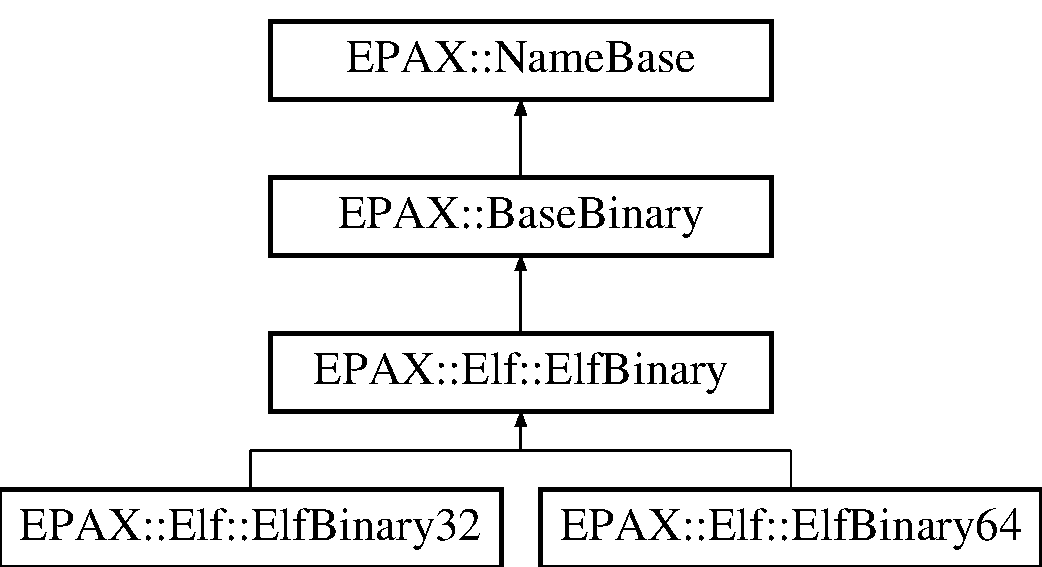
\includegraphics[height=4.000000cm]{class_e_p_a_x_1_1_elf_1_1_elf_binary}
\end{center}
\end{figure}
\subsection*{\-Public \-Member \-Functions}
\begin{DoxyCompactItemize}
\item 
\hyperlink{class_e_p_a_x_1_1_elf_1_1_elf_binary_aea424db302d99d3330aa5c6331834a45}{\-Elf\-Binary} (std\-::string n)
\item 
virtual \hyperlink{class_e_p_a_x_1_1_elf_1_1_elf_binary_ab7e61b25803a678994e693ce134c9389}{$\sim$\-Elf\-Binary} ()
\item 
virtual \hyperlink{namespace_e_p_a_x_a4be639c006ef14def4708b37ee6dd67d}{\-Binary\-Format} \hyperlink{class_e_p_a_x_1_1_elf_1_1_elf_binary_a2f8cfe8d4567e4aefbeb0717da3f0e9c}{get\-Format} ()=0
\item 
uint64\-\_\-t \hyperlink{class_e_p_a_x_1_1_elf_1_1_elf_binary_af4d56ab5e4f25b17f236c1712dd7c2bb}{get\-Start\-Addr} ()
\item 
void \hyperlink{class_e_p_a_x_1_1_elf_1_1_elf_binary_ac929a0c398ce61c8ac80df79dbb6a1d9}{emit} (std\-::string n)
\item 
bool \hyperlink{class_e_p_a_x_1_1_elf_1_1_elf_binary_a9955c801d73bcc62ce60a884f4d36464}{verify} ()
\item 
bool \hyperlink{class_e_p_a_x_1_1_elf_1_1_elf_binary_a48ca78d2f324eef54c478532d1d38636}{is\-A\-R\-M} ()
\item 
void \hyperlink{class_e_p_a_x_1_1_elf_1_1_elf_binary_aa6846ae0eedb4620e26e3b466efec629}{describe} ()
\item 
void \hyperlink{class_e_p_a_x_1_1_elf_1_1_elf_binary_a57b3bc6b92a7964835e424d610523240}{find\-Functions} ()
\item 
void \hyperlink{class_e_p_a_x_1_1_elf_1_1_elf_binary_a393e4e2eeea3224d1b61c6a8412c9da5}{find\-Symbols} ()
\item 
void \hyperlink{class_e_p_a_x_1_1_elf_1_1_elf_binary_ad4a57cb23543cb8b37d9b4fa61f07a0c}{find\-Sections} ()
\item 
void \hyperlink{class_e_p_a_x_1_1_elf_1_1_elf_binary_ae357dea8fe42fff9b8ae321dc94b0503}{find\-Segments} ()
\item 
bool \hyperlink{class_e_p_a_x_1_1_elf_1_1_elf_binary_a813a2985bd91b6e7640a2221235fdb4e}{is32\-Bit} ()
\item 
bool \hyperlink{class_e_p_a_x_1_1_elf_1_1_elf_binary_a07de5ed756446ede40d3f1328eedfa0b}{is64\-Bit} ()
\item 
bool \hyperlink{class_e_p_a_x_1_1_elf_1_1_elf_binary_a683bf66639d6fb4c4d9e9904a563494e}{is\-Executable} ()
\item 
\hyperlink{class_e_p_a_x_1_1_elf_1_1_elf_string_table}{\-Elf\-String\-Table} $\ast$ \hyperlink{class_e_p_a_x_1_1_elf_1_1_elf_binary_ae14d70c8ea2a3e9eaa1be65661c56efb}{find\-Stringtable} (uint32\-\_\-t i)
\item 
bool \hyperlink{class_e_p_a_x_1_1_elf_1_1_elf_binary_ae52abd95dd6d7f77d3e6da0e629c86e5}{inside\-Text\-Range} (uint64\-\_\-t a)
\item 
void \hyperlink{class_e_p_a_x_1_1_elf_1_1_elf_binary_ae200e871cf5c040ed1d8ed074eb1e5c2}{print\-Sections} (std\-::ostream \&stream=std\-::cout)
\item 
void \hyperlink{class_e_p_a_x_1_1_elf_1_1_elf_binary_aac1eb1e8571502f6005ac54d4b6e5920}{print\-Functions} (std\-::ostream \&stream=std\-::cout)
\item 
uint64\-\_\-t \hyperlink{class_e_p_a_x_1_1_elf_1_1_elf_binary_add93e2899e35ec753660479b1aa6969f}{vaddr\-To\-File} (uint64\-\_\-t v)
\item 
uint64\-\_\-t \hyperlink{class_e_p_a_x_1_1_elf_1_1_elf_binary_a7cba4b5796d98043e281f46437abb6d9}{function\-End\-Address} (\hyperlink{class_e_p_a_x_1_1_function}{\-Function} $\ast$f, \hyperlink{class_e_p_a_x_1_1_function}{\-Function} $\ast$nextf)
\end{DoxyCompactItemize}
\subsection*{\-Protected \-Attributes}
\begin{DoxyCompactItemize}
\item 
\hyperlink{class_e_p_a_x_1_1_elf_1_1_file_header}{\-File\-Header} $\ast$ \hyperlink{class_e_p_a_x_1_1_elf_1_1_elf_binary_aa0f3e41ca81ccff7704a1a25d2ec3a45}{fileheader}
\item 
bool \hyperlink{class_e_p_a_x_1_1_elf_1_1_elf_binary_a0fff68c4ab05d176acf716fc878a20ab}{foundsections}
\item 
std\-::vector$<$ \hyperlink{class_e_p_a_x_1_1_elf_1_1_section_header}{\-Section\-Header} $\ast$ $>$ $\ast$ \hyperlink{class_e_p_a_x_1_1_elf_1_1_elf_binary_afbb96059b56ec958d3901a1562343224}{sections}
\item 
bool \hyperlink{class_e_p_a_x_1_1_elf_1_1_elf_binary_a07d9f4abb56b2522a17f6db39373a53a}{foundsegments}
\item 
std\-::vector$<$ \hyperlink{class_e_p_a_x_1_1_elf_1_1_program_header}{\-Program\-Header} $\ast$ $>$ $\ast$ \hyperlink{class_e_p_a_x_1_1_elf_1_1_elf_binary_a75dbde6b29cdcd5297e18645c165d7d5}{segments}
\end{DoxyCompactItemize}


\subsection{\-Detailed \-Description}


\-Definition at line 42 of file \-Elf\-Binary.\-hpp.



\subsection{\-Constructor \& \-Destructor \-Documentation}
\hypertarget{class_e_p_a_x_1_1_elf_1_1_elf_binary_aea424db302d99d3330aa5c6331834a45}{\index{\-E\-P\-A\-X\-::\-Elf\-::\-Elf\-Binary@{\-E\-P\-A\-X\-::\-Elf\-::\-Elf\-Binary}!\-Elf\-Binary@{\-Elf\-Binary}}
\index{\-Elf\-Binary@{\-Elf\-Binary}!EPAX::Elf::ElfBinary@{\-E\-P\-A\-X\-::\-Elf\-::\-Elf\-Binary}}
\subsubsection[{\-Elf\-Binary}]{\setlength{\rightskip}{0pt plus 5cm}{\bf \-E\-P\-A\-X\-::\-Elf\-::\-Elf\-Binary\-::\-Elf\-Binary} (
\begin{DoxyParamCaption}
\item[{std\-::string}]{n}
\end{DoxyParamCaption}
)}}\label{class_e_p_a_x_1_1_elf_1_1_elf_binary_aea424db302d99d3330aa5c6331834a45}


\-Definition at line 47 of file \-Elf\-Binary.\-cpp.

\hypertarget{class_e_p_a_x_1_1_elf_1_1_elf_binary_ab7e61b25803a678994e693ce134c9389}{\index{\-E\-P\-A\-X\-::\-Elf\-::\-Elf\-Binary@{\-E\-P\-A\-X\-::\-Elf\-::\-Elf\-Binary}!$\sim$\-Elf\-Binary@{$\sim$\-Elf\-Binary}}
\index{$\sim$\-Elf\-Binary@{$\sim$\-Elf\-Binary}!EPAX::Elf::ElfBinary@{\-E\-P\-A\-X\-::\-Elf\-::\-Elf\-Binary}}
\subsubsection[{$\sim$\-Elf\-Binary}]{\setlength{\rightskip}{0pt plus 5cm}{\bf \-E\-P\-A\-X\-::\-Elf\-::\-Elf\-Binary\-::$\sim$\-Elf\-Binary} (
\begin{DoxyParamCaption}
{}
\end{DoxyParamCaption}
)\hspace{0.3cm}{\ttfamily  \mbox{[}virtual\mbox{]}}}}\label{class_e_p_a_x_1_1_elf_1_1_elf_binary_ab7e61b25803a678994e693ce134c9389}


\-Definition at line 55 of file \-Elf\-Binary.\-cpp.



\subsection{\-Member \-Function \-Documentation}
\hypertarget{class_e_p_a_x_1_1_elf_1_1_elf_binary_aa6846ae0eedb4620e26e3b466efec629}{\index{\-E\-P\-A\-X\-::\-Elf\-::\-Elf\-Binary@{\-E\-P\-A\-X\-::\-Elf\-::\-Elf\-Binary}!describe@{describe}}
\index{describe@{describe}!EPAX::Elf::ElfBinary@{\-E\-P\-A\-X\-::\-Elf\-::\-Elf\-Binary}}
\subsubsection[{describe}]{\setlength{\rightskip}{0pt plus 5cm}void {\bf \-E\-P\-A\-X\-::\-Elf\-::\-Elf\-Binary\-::describe} (
\begin{DoxyParamCaption}
{}
\end{DoxyParamCaption}
)\hspace{0.3cm}{\ttfamily  \mbox{[}virtual\mbox{]}}}}\label{class_e_p_a_x_1_1_elf_1_1_elf_binary_aa6846ae0eedb4620e26e3b466efec629}


\-Implements \hyperlink{class_e_p_a_x_1_1_base_binary_a501175cac7fb1650bf378d6b4729c1ec}{\-E\-P\-A\-X\-::\-Base\-Binary}.



\-Definition at line 120 of file \-Elf\-Binary.\-cpp.

\hypertarget{class_e_p_a_x_1_1_elf_1_1_elf_binary_ac929a0c398ce61c8ac80df79dbb6a1d9}{\index{\-E\-P\-A\-X\-::\-Elf\-::\-Elf\-Binary@{\-E\-P\-A\-X\-::\-Elf\-::\-Elf\-Binary}!emit@{emit}}
\index{emit@{emit}!EPAX::Elf::ElfBinary@{\-E\-P\-A\-X\-::\-Elf\-::\-Elf\-Binary}}
\subsubsection[{emit}]{\setlength{\rightskip}{0pt plus 5cm}void {\bf \-E\-P\-A\-X\-::\-Elf\-::\-Elf\-Binary\-::emit} (
\begin{DoxyParamCaption}
\item[{std\-::string}]{n}
\end{DoxyParamCaption}
)\hspace{0.3cm}{\ttfamily  \mbox{[}virtual\mbox{]}}}}\label{class_e_p_a_x_1_1_elf_1_1_elf_binary_ac929a0c398ce61c8ac80df79dbb6a1d9}


\-Implements \hyperlink{class_e_p_a_x_1_1_base_binary_a8883d3b0580cae0f5a1960c6fbfd6a1f}{\-E\-P\-A\-X\-::\-Base\-Binary}.



\-Definition at line 144 of file \-Elf\-Binary.\-cpp.

\hypertarget{class_e_p_a_x_1_1_elf_1_1_elf_binary_a57b3bc6b92a7964835e424d610523240}{\index{\-E\-P\-A\-X\-::\-Elf\-::\-Elf\-Binary@{\-E\-P\-A\-X\-::\-Elf\-::\-Elf\-Binary}!find\-Functions@{find\-Functions}}
\index{find\-Functions@{find\-Functions}!EPAX::Elf::ElfBinary@{\-E\-P\-A\-X\-::\-Elf\-::\-Elf\-Binary}}
\subsubsection[{find\-Functions}]{\setlength{\rightskip}{0pt plus 5cm}void {\bf \-E\-P\-A\-X\-::\-Elf\-::\-Elf\-Binary\-::find\-Functions} (
\begin{DoxyParamCaption}
{}
\end{DoxyParamCaption}
)\hspace{0.3cm}{\ttfamily  \mbox{[}virtual\mbox{]}}}}\label{class_e_p_a_x_1_1_elf_1_1_elf_binary_a57b3bc6b92a7964835e424d610523240}
\-Finds and internally stores all functions in the image

\begin{DoxyReturn}{\-Returns}
none 
\end{DoxyReturn}


\-Implements \hyperlink{class_e_p_a_x_1_1_base_binary_abcd76218158ab20a2f81d68a537b21cb}{\-E\-P\-A\-X\-::\-Base\-Binary}.



\-Definition at line 158 of file \-Elf\-Binary.\-cpp.

\hypertarget{class_e_p_a_x_1_1_elf_1_1_elf_binary_ad4a57cb23543cb8b37d9b4fa61f07a0c}{\index{\-E\-P\-A\-X\-::\-Elf\-::\-Elf\-Binary@{\-E\-P\-A\-X\-::\-Elf\-::\-Elf\-Binary}!find\-Sections@{find\-Sections}}
\index{find\-Sections@{find\-Sections}!EPAX::Elf::ElfBinary@{\-E\-P\-A\-X\-::\-Elf\-::\-Elf\-Binary}}
\subsubsection[{find\-Sections}]{\setlength{\rightskip}{0pt plus 5cm}void {\bf \-E\-P\-A\-X\-::\-Elf\-::\-Elf\-Binary\-::find\-Sections} (
\begin{DoxyParamCaption}
{}
\end{DoxyParamCaption}
)}}\label{class_e_p_a_x_1_1_elf_1_1_elf_binary_ad4a57cb23543cb8b37d9b4fa61f07a0c}


\-Definition at line 278 of file \-Elf\-Binary.\-cpp.

\hypertarget{class_e_p_a_x_1_1_elf_1_1_elf_binary_ae357dea8fe42fff9b8ae321dc94b0503}{\index{\-E\-P\-A\-X\-::\-Elf\-::\-Elf\-Binary@{\-E\-P\-A\-X\-::\-Elf\-::\-Elf\-Binary}!find\-Segments@{find\-Segments}}
\index{find\-Segments@{find\-Segments}!EPAX::Elf::ElfBinary@{\-E\-P\-A\-X\-::\-Elf\-::\-Elf\-Binary}}
\subsubsection[{find\-Segments}]{\setlength{\rightskip}{0pt plus 5cm}void {\bf \-E\-P\-A\-X\-::\-Elf\-::\-Elf\-Binary\-::find\-Segments} (
\begin{DoxyParamCaption}
{}
\end{DoxyParamCaption}
)}}\label{class_e_p_a_x_1_1_elf_1_1_elf_binary_ae357dea8fe42fff9b8ae321dc94b0503}


\-Definition at line 299 of file \-Elf\-Binary.\-cpp.

\hypertarget{class_e_p_a_x_1_1_elf_1_1_elf_binary_ae14d70c8ea2a3e9eaa1be65661c56efb}{\index{\-E\-P\-A\-X\-::\-Elf\-::\-Elf\-Binary@{\-E\-P\-A\-X\-::\-Elf\-::\-Elf\-Binary}!find\-Stringtable@{find\-Stringtable}}
\index{find\-Stringtable@{find\-Stringtable}!EPAX::Elf::ElfBinary@{\-E\-P\-A\-X\-::\-Elf\-::\-Elf\-Binary}}
\subsubsection[{find\-Stringtable}]{\setlength{\rightskip}{0pt plus 5cm}{\bf \-Elf\-String\-Table} $\ast$ {\bf \-E\-P\-A\-X\-::\-Elf\-::\-Elf\-Binary\-::find\-Stringtable} (
\begin{DoxyParamCaption}
\item[{uint32\-\_\-t}]{i}
\end{DoxyParamCaption}
)}}\label{class_e_p_a_x_1_1_elf_1_1_elf_binary_ae14d70c8ea2a3e9eaa1be65661c56efb}


\-Definition at line 220 of file \-Elf\-Binary.\-cpp.

\hypertarget{class_e_p_a_x_1_1_elf_1_1_elf_binary_a393e4e2eeea3224d1b61c6a8412c9da5}{\index{\-E\-P\-A\-X\-::\-Elf\-::\-Elf\-Binary@{\-E\-P\-A\-X\-::\-Elf\-::\-Elf\-Binary}!find\-Symbols@{find\-Symbols}}
\index{find\-Symbols@{find\-Symbols}!EPAX::Elf::ElfBinary@{\-E\-P\-A\-X\-::\-Elf\-::\-Elf\-Binary}}
\subsubsection[{find\-Symbols}]{\setlength{\rightskip}{0pt plus 5cm}void {\bf \-E\-P\-A\-X\-::\-Elf\-::\-Elf\-Binary\-::find\-Symbols} (
\begin{DoxyParamCaption}
{}
\end{DoxyParamCaption}
)\hspace{0.3cm}{\ttfamily  \mbox{[}virtual\mbox{]}}}}\label{class_e_p_a_x_1_1_elf_1_1_elf_binary_a393e4e2eeea3224d1b61c6a8412c9da5}
\-Finds and internally stores all symbols in the image

\begin{DoxyReturn}{\-Returns}
none 
\end{DoxyReturn}


\-Implements \hyperlink{class_e_p_a_x_1_1_base_binary_adc22abd64f6a873fbce30c79508322fe}{\-E\-P\-A\-X\-::\-Base\-Binary}.



\-Definition at line 230 of file \-Elf\-Binary.\-cpp.

\hypertarget{class_e_p_a_x_1_1_elf_1_1_elf_binary_a7cba4b5796d98043e281f46437abb6d9}{\index{\-E\-P\-A\-X\-::\-Elf\-::\-Elf\-Binary@{\-E\-P\-A\-X\-::\-Elf\-::\-Elf\-Binary}!function\-End\-Address@{function\-End\-Address}}
\index{function\-End\-Address@{function\-End\-Address}!EPAX::Elf::ElfBinary@{\-E\-P\-A\-X\-::\-Elf\-::\-Elf\-Binary}}
\subsubsection[{function\-End\-Address}]{\setlength{\rightskip}{0pt plus 5cm}uint64\-\_\-t {\bf \-E\-P\-A\-X\-::\-Elf\-::\-Elf\-Binary\-::function\-End\-Address} (
\begin{DoxyParamCaption}
\item[{{\bf \-Function} $\ast$}]{f, }
\item[{{\bf \-Function} $\ast$}]{nextf}
\end{DoxyParamCaption}
)\hspace{0.3cm}{\ttfamily  \mbox{[}virtual\mbox{]}}}}\label{class_e_p_a_x_1_1_elf_1_1_elf_binary_a7cba4b5796d98043e281f46437abb6d9}


\-Implements \hyperlink{class_e_p_a_x_1_1_base_binary_a3ebaa616622aaca98685ece5d59c05d8}{\-E\-P\-A\-X\-::\-Base\-Binary}.



\-Definition at line 88 of file \-Elf\-Binary.\-cpp.

\hypertarget{class_e_p_a_x_1_1_elf_1_1_elf_binary_a2f8cfe8d4567e4aefbeb0717da3f0e9c}{\index{\-E\-P\-A\-X\-::\-Elf\-::\-Elf\-Binary@{\-E\-P\-A\-X\-::\-Elf\-::\-Elf\-Binary}!get\-Format@{get\-Format}}
\index{get\-Format@{get\-Format}!EPAX::Elf::ElfBinary@{\-E\-P\-A\-X\-::\-Elf\-::\-Elf\-Binary}}
\subsubsection[{get\-Format}]{\setlength{\rightskip}{0pt plus 5cm}virtual {\bf \-Binary\-Format} {\bf \-E\-P\-A\-X\-::\-Elf\-::\-Elf\-Binary\-::get\-Format} (
\begin{DoxyParamCaption}
{}
\end{DoxyParamCaption}
)\hspace{0.3cm}{\ttfamily  \mbox{[}pure virtual\mbox{]}}}}\label{class_e_p_a_x_1_1_elf_1_1_elf_binary_a2f8cfe8d4567e4aefbeb0717da3f0e9c}


\-Implements \hyperlink{class_e_p_a_x_1_1_base_binary_a456741cd16605e5035ab89ab813f4373}{\-E\-P\-A\-X\-::\-Base\-Binary}.



\-Implemented in \hyperlink{class_e_p_a_x_1_1_elf_1_1_elf_binary64_a8d4ac63ef8a488fb6ad98fd24ad36d07}{\-E\-P\-A\-X\-::\-Elf\-::\-Elf\-Binary64}, and \hyperlink{class_e_p_a_x_1_1_elf_1_1_elf_binary32_ad3c232fe03109e9a59e5456420d4fed3}{\-E\-P\-A\-X\-::\-Elf\-::\-Elf\-Binary32}.

\hypertarget{class_e_p_a_x_1_1_elf_1_1_elf_binary_af4d56ab5e4f25b17f236c1712dd7c2bb}{\index{\-E\-P\-A\-X\-::\-Elf\-::\-Elf\-Binary@{\-E\-P\-A\-X\-::\-Elf\-::\-Elf\-Binary}!get\-Start\-Addr@{get\-Start\-Addr}}
\index{get\-Start\-Addr@{get\-Start\-Addr}!EPAX::Elf::ElfBinary@{\-E\-P\-A\-X\-::\-Elf\-::\-Elf\-Binary}}
\subsubsection[{get\-Start\-Addr}]{\setlength{\rightskip}{0pt plus 5cm}uint64\-\_\-t {\bf \-E\-P\-A\-X\-::\-Elf\-::\-Elf\-Binary\-::get\-Start\-Addr} (
\begin{DoxyParamCaption}
{}
\end{DoxyParamCaption}
)\hspace{0.3cm}{\ttfamily  \mbox{[}virtual\mbox{]}}}}\label{class_e_p_a_x_1_1_elf_1_1_elf_binary_af4d56ab5e4f25b17f236c1712dd7c2bb}


\-Implements \hyperlink{class_e_p_a_x_1_1_base_binary_ad23fe3f3a6f5b387df2f4eb7e4a4f23d}{\-E\-P\-A\-X\-::\-Base\-Binary}.



\-Definition at line 108 of file \-Elf\-Binary.\-cpp.

\hypertarget{class_e_p_a_x_1_1_elf_1_1_elf_binary_ae52abd95dd6d7f77d3e6da0e629c86e5}{\index{\-E\-P\-A\-X\-::\-Elf\-::\-Elf\-Binary@{\-E\-P\-A\-X\-::\-Elf\-::\-Elf\-Binary}!inside\-Text\-Range@{inside\-Text\-Range}}
\index{inside\-Text\-Range@{inside\-Text\-Range}!EPAX::Elf::ElfBinary@{\-E\-P\-A\-X\-::\-Elf\-::\-Elf\-Binary}}
\subsubsection[{inside\-Text\-Range}]{\setlength{\rightskip}{0pt plus 5cm}bool {\bf \-E\-P\-A\-X\-::\-Elf\-::\-Elf\-Binary\-::inside\-Text\-Range} (
\begin{DoxyParamCaption}
\item[{uint64\-\_\-t}]{a}
\end{DoxyParamCaption}
)\hspace{0.3cm}{\ttfamily  \mbox{[}virtual\mbox{]}}}}\label{class_e_p_a_x_1_1_elf_1_1_elf_binary_ae52abd95dd6d7f77d3e6da0e629c86e5}


\-Implements \hyperlink{class_e_p_a_x_1_1_base_binary_aa0f29bfa881c2199911465c64e421be6}{\-E\-P\-A\-X\-::\-Base\-Binary}.



\-Definition at line 78 of file \-Elf\-Binary.\-cpp.

\hypertarget{class_e_p_a_x_1_1_elf_1_1_elf_binary_a813a2985bd91b6e7640a2221235fdb4e}{\index{\-E\-P\-A\-X\-::\-Elf\-::\-Elf\-Binary@{\-E\-P\-A\-X\-::\-Elf\-::\-Elf\-Binary}!is32\-Bit@{is32\-Bit}}
\index{is32\-Bit@{is32\-Bit}!EPAX::Elf::ElfBinary@{\-E\-P\-A\-X\-::\-Elf\-::\-Elf\-Binary}}
\subsubsection[{is32\-Bit}]{\setlength{\rightskip}{0pt plus 5cm}bool {\bf \-E\-P\-A\-X\-::\-Elf\-::\-Elf\-Binary\-::is32\-Bit} (
\begin{DoxyParamCaption}
{}
\end{DoxyParamCaption}
)\hspace{0.3cm}{\ttfamily  \mbox{[}virtual\mbox{]}}}}\label{class_e_p_a_x_1_1_elf_1_1_elf_binary_a813a2985bd91b6e7640a2221235fdb4e}


\-Implements \hyperlink{class_e_p_a_x_1_1_base_binary_ac71bc6c28fe40456ddf626a8bbca257f}{\-E\-P\-A\-X\-::\-Base\-Binary}.



\-Definition at line 136 of file \-Elf\-Binary.\-cpp.

\hypertarget{class_e_p_a_x_1_1_elf_1_1_elf_binary_a07de5ed756446ede40d3f1328eedfa0b}{\index{\-E\-P\-A\-X\-::\-Elf\-::\-Elf\-Binary@{\-E\-P\-A\-X\-::\-Elf\-::\-Elf\-Binary}!is64\-Bit@{is64\-Bit}}
\index{is64\-Bit@{is64\-Bit}!EPAX::Elf::ElfBinary@{\-E\-P\-A\-X\-::\-Elf\-::\-Elf\-Binary}}
\subsubsection[{is64\-Bit}]{\setlength{\rightskip}{0pt plus 5cm}bool {\bf \-E\-P\-A\-X\-::\-Elf\-::\-Elf\-Binary\-::is64\-Bit} (
\begin{DoxyParamCaption}
{}
\end{DoxyParamCaption}
)\hspace{0.3cm}{\ttfamily  \mbox{[}virtual\mbox{]}}}}\label{class_e_p_a_x_1_1_elf_1_1_elf_binary_a07de5ed756446ede40d3f1328eedfa0b}


\-Implements \hyperlink{class_e_p_a_x_1_1_base_binary_a303cdafe0782ed63d8115bc225f169ee}{\-E\-P\-A\-X\-::\-Base\-Binary}.



\-Definition at line 140 of file \-Elf\-Binary.\-cpp.

\hypertarget{class_e_p_a_x_1_1_elf_1_1_elf_binary_a48ca78d2f324eef54c478532d1d38636}{\index{\-E\-P\-A\-X\-::\-Elf\-::\-Elf\-Binary@{\-E\-P\-A\-X\-::\-Elf\-::\-Elf\-Binary}!is\-A\-R\-M@{is\-A\-R\-M}}
\index{is\-A\-R\-M@{is\-A\-R\-M}!EPAX::Elf::ElfBinary@{\-E\-P\-A\-X\-::\-Elf\-::\-Elf\-Binary}}
\subsubsection[{is\-A\-R\-M}]{\setlength{\rightskip}{0pt plus 5cm}bool {\bf \-E\-P\-A\-X\-::\-Elf\-::\-Elf\-Binary\-::is\-A\-R\-M} (
\begin{DoxyParamCaption}
{}
\end{DoxyParamCaption}
)\hspace{0.3cm}{\ttfamily  \mbox{[}virtual\mbox{]}}}}\label{class_e_p_a_x_1_1_elf_1_1_elf_binary_a48ca78d2f324eef54c478532d1d38636}


\-Implements \hyperlink{class_e_p_a_x_1_1_base_binary_ac544fc0d096ca8a555b30fe7126ae846}{\-E\-P\-A\-X\-::\-Base\-Binary}.



\-Definition at line 116 of file \-Elf\-Binary.\-cpp.

\hypertarget{class_e_p_a_x_1_1_elf_1_1_elf_binary_a683bf66639d6fb4c4d9e9904a563494e}{\index{\-E\-P\-A\-X\-::\-Elf\-::\-Elf\-Binary@{\-E\-P\-A\-X\-::\-Elf\-::\-Elf\-Binary}!is\-Executable@{is\-Executable}}
\index{is\-Executable@{is\-Executable}!EPAX::Elf::ElfBinary@{\-E\-P\-A\-X\-::\-Elf\-::\-Elf\-Binary}}
\subsubsection[{is\-Executable}]{\setlength{\rightskip}{0pt plus 5cm}bool {\bf \-E\-P\-A\-X\-::\-Elf\-::\-Elf\-Binary\-::is\-Executable} (
\begin{DoxyParamCaption}
{}
\end{DoxyParamCaption}
)\hspace{0.3cm}{\ttfamily  \mbox{[}virtual\mbox{]}}}}\label{class_e_p_a_x_1_1_elf_1_1_elf_binary_a683bf66639d6fb4c4d9e9904a563494e}


\-Implements \hyperlink{class_e_p_a_x_1_1_base_binary_aeeb90ae234b0f661ef387ee31d3c4762}{\-E\-P\-A\-X\-::\-Base\-Binary}.



\-Definition at line 458 of file \-Elf\-Binary.\-cpp.

\hypertarget{class_e_p_a_x_1_1_elf_1_1_elf_binary_aac1eb1e8571502f6005ac54d4b6e5920}{\index{\-E\-P\-A\-X\-::\-Elf\-::\-Elf\-Binary@{\-E\-P\-A\-X\-::\-Elf\-::\-Elf\-Binary}!print\-Functions@{print\-Functions}}
\index{print\-Functions@{print\-Functions}!EPAX::Elf::ElfBinary@{\-E\-P\-A\-X\-::\-Elf\-::\-Elf\-Binary}}
\subsubsection[{print\-Functions}]{\setlength{\rightskip}{0pt plus 5cm}void {\bf \-E\-P\-A\-X\-::\-Elf\-::\-Elf\-Binary\-::print\-Functions} (
\begin{DoxyParamCaption}
\item[{std\-::ostream \&}]{stream = {\ttfamily std\-:\-:cout}}
\end{DoxyParamCaption}
)\hspace{0.3cm}{\ttfamily  \mbox{[}virtual\mbox{]}}}}\label{class_e_p_a_x_1_1_elf_1_1_elf_binary_aac1eb1e8571502f6005ac54d4b6e5920}


\-Implements \hyperlink{class_e_p_a_x_1_1_base_binary_a879d43acc68de4f468c26d5cfe4ab59d}{\-E\-P\-A\-X\-::\-Base\-Binary}.



\-Definition at line 210 of file \-Elf\-Binary.\-cpp.

\hypertarget{class_e_p_a_x_1_1_elf_1_1_elf_binary_ae200e871cf5c040ed1d8ed074eb1e5c2}{\index{\-E\-P\-A\-X\-::\-Elf\-::\-Elf\-Binary@{\-E\-P\-A\-X\-::\-Elf\-::\-Elf\-Binary}!print\-Sections@{print\-Sections}}
\index{print\-Sections@{print\-Sections}!EPAX::Elf::ElfBinary@{\-E\-P\-A\-X\-::\-Elf\-::\-Elf\-Binary}}
\subsubsection[{print\-Sections}]{\setlength{\rightskip}{0pt plus 5cm}void {\bf \-E\-P\-A\-X\-::\-Elf\-::\-Elf\-Binary\-::print\-Sections} (
\begin{DoxyParamCaption}
\item[{std\-::ostream \&}]{stream = {\ttfamily std\-:\-:cout}}
\end{DoxyParamCaption}
)\hspace{0.3cm}{\ttfamily  \mbox{[}virtual\mbox{]}}}}\label{class_e_p_a_x_1_1_elf_1_1_elf_binary_ae200e871cf5c040ed1d8ed074eb1e5c2}


\-Implements \hyperlink{class_e_p_a_x_1_1_base_binary_a9ef8978bbd895a198b68cc04974c57cc}{\-E\-P\-A\-X\-::\-Base\-Binary}.



\-Definition at line 704 of file \-Elf\-Binary.\-cpp.

\hypertarget{class_e_p_a_x_1_1_elf_1_1_elf_binary_add93e2899e35ec753660479b1aa6969f}{\index{\-E\-P\-A\-X\-::\-Elf\-::\-Elf\-Binary@{\-E\-P\-A\-X\-::\-Elf\-::\-Elf\-Binary}!vaddr\-To\-File@{vaddr\-To\-File}}
\index{vaddr\-To\-File@{vaddr\-To\-File}!EPAX::Elf::ElfBinary@{\-E\-P\-A\-X\-::\-Elf\-::\-Elf\-Binary}}
\subsubsection[{vaddr\-To\-File}]{\setlength{\rightskip}{0pt plus 5cm}uint64\-\_\-t {\bf \-E\-P\-A\-X\-::\-Elf\-::\-Elf\-Binary\-::vaddr\-To\-File} (
\begin{DoxyParamCaption}
\item[{uint64\-\_\-t}]{v}
\end{DoxyParamCaption}
)}}\label{class_e_p_a_x_1_1_elf_1_1_elf_binary_add93e2899e35ec753660479b1aa6969f}


\-Definition at line 148 of file \-Elf\-Binary.\-cpp.

\hypertarget{class_e_p_a_x_1_1_elf_1_1_elf_binary_a9955c801d73bcc62ce60a884f4d36464}{\index{\-E\-P\-A\-X\-::\-Elf\-::\-Elf\-Binary@{\-E\-P\-A\-X\-::\-Elf\-::\-Elf\-Binary}!verify@{verify}}
\index{verify@{verify}!EPAX::Elf::ElfBinary@{\-E\-P\-A\-X\-::\-Elf\-::\-Elf\-Binary}}
\subsubsection[{verify}]{\setlength{\rightskip}{0pt plus 5cm}bool {\bf \-E\-P\-A\-X\-::\-Elf\-::\-Elf\-Binary\-::verify} (
\begin{DoxyParamCaption}
{}
\end{DoxyParamCaption}
)\hspace{0.3cm}{\ttfamily  \mbox{[}virtual\mbox{]}}}}\label{class_e_p_a_x_1_1_elf_1_1_elf_binary_a9955c801d73bcc62ce60a884f4d36464}


\-Implements \hyperlink{class_e_p_a_x_1_1_base_binary_a3e00d0fecc2defaab16a3ee4b72a32ca}{\-E\-P\-A\-X\-::\-Base\-Binary}.



\-Definition at line 112 of file \-Elf\-Binary.\-cpp.



\subsection{\-Member \-Data \-Documentation}
\hypertarget{class_e_p_a_x_1_1_elf_1_1_elf_binary_aa0f3e41ca81ccff7704a1a25d2ec3a45}{\index{\-E\-P\-A\-X\-::\-Elf\-::\-Elf\-Binary@{\-E\-P\-A\-X\-::\-Elf\-::\-Elf\-Binary}!fileheader@{fileheader}}
\index{fileheader@{fileheader}!EPAX::Elf::ElfBinary@{\-E\-P\-A\-X\-::\-Elf\-::\-Elf\-Binary}}
\subsubsection[{fileheader}]{\setlength{\rightskip}{0pt plus 5cm}{\bf \-File\-Header}$\ast$ {\bf \-E\-P\-A\-X\-::\-Elf\-::\-Elf\-Binary\-::fileheader}\hspace{0.3cm}{\ttfamily  \mbox{[}protected\mbox{]}}}}\label{class_e_p_a_x_1_1_elf_1_1_elf_binary_aa0f3e41ca81ccff7704a1a25d2ec3a45}


\-Definition at line 44 of file \-Elf\-Binary.\-hpp.

\hypertarget{class_e_p_a_x_1_1_elf_1_1_elf_binary_a0fff68c4ab05d176acf716fc878a20ab}{\index{\-E\-P\-A\-X\-::\-Elf\-::\-Elf\-Binary@{\-E\-P\-A\-X\-::\-Elf\-::\-Elf\-Binary}!foundsections@{foundsections}}
\index{foundsections@{foundsections}!EPAX::Elf::ElfBinary@{\-E\-P\-A\-X\-::\-Elf\-::\-Elf\-Binary}}
\subsubsection[{foundsections}]{\setlength{\rightskip}{0pt plus 5cm}bool {\bf \-E\-P\-A\-X\-::\-Elf\-::\-Elf\-Binary\-::foundsections}\hspace{0.3cm}{\ttfamily  \mbox{[}protected\mbox{]}}}}\label{class_e_p_a_x_1_1_elf_1_1_elf_binary_a0fff68c4ab05d176acf716fc878a20ab}


\-Definition at line 46 of file \-Elf\-Binary.\-hpp.

\hypertarget{class_e_p_a_x_1_1_elf_1_1_elf_binary_a07d9f4abb56b2522a17f6db39373a53a}{\index{\-E\-P\-A\-X\-::\-Elf\-::\-Elf\-Binary@{\-E\-P\-A\-X\-::\-Elf\-::\-Elf\-Binary}!foundsegments@{foundsegments}}
\index{foundsegments@{foundsegments}!EPAX::Elf::ElfBinary@{\-E\-P\-A\-X\-::\-Elf\-::\-Elf\-Binary}}
\subsubsection[{foundsegments}]{\setlength{\rightskip}{0pt plus 5cm}bool {\bf \-E\-P\-A\-X\-::\-Elf\-::\-Elf\-Binary\-::foundsegments}\hspace{0.3cm}{\ttfamily  \mbox{[}protected\mbox{]}}}}\label{class_e_p_a_x_1_1_elf_1_1_elf_binary_a07d9f4abb56b2522a17f6db39373a53a}


\-Definition at line 48 of file \-Elf\-Binary.\-hpp.

\hypertarget{class_e_p_a_x_1_1_elf_1_1_elf_binary_afbb96059b56ec958d3901a1562343224}{\index{\-E\-P\-A\-X\-::\-Elf\-::\-Elf\-Binary@{\-E\-P\-A\-X\-::\-Elf\-::\-Elf\-Binary}!sections@{sections}}
\index{sections@{sections}!EPAX::Elf::ElfBinary@{\-E\-P\-A\-X\-::\-Elf\-::\-Elf\-Binary}}
\subsubsection[{sections}]{\setlength{\rightskip}{0pt plus 5cm}std\-::vector$<${\bf \-Section\-Header}$\ast$$>$$\ast$ {\bf \-E\-P\-A\-X\-::\-Elf\-::\-Elf\-Binary\-::sections}\hspace{0.3cm}{\ttfamily  \mbox{[}protected\mbox{]}}}}\label{class_e_p_a_x_1_1_elf_1_1_elf_binary_afbb96059b56ec958d3901a1562343224}


\-Definition at line 47 of file \-Elf\-Binary.\-hpp.

\hypertarget{class_e_p_a_x_1_1_elf_1_1_elf_binary_a75dbde6b29cdcd5297e18645c165d7d5}{\index{\-E\-P\-A\-X\-::\-Elf\-::\-Elf\-Binary@{\-E\-P\-A\-X\-::\-Elf\-::\-Elf\-Binary}!segments@{segments}}
\index{segments@{segments}!EPAX::Elf::ElfBinary@{\-E\-P\-A\-X\-::\-Elf\-::\-Elf\-Binary}}
\subsubsection[{segments}]{\setlength{\rightskip}{0pt plus 5cm}std\-::vector$<${\bf \-Program\-Header}$\ast$$>$$\ast$ {\bf \-E\-P\-A\-X\-::\-Elf\-::\-Elf\-Binary\-::segments}\hspace{0.3cm}{\ttfamily  \mbox{[}protected\mbox{]}}}}\label{class_e_p_a_x_1_1_elf_1_1_elf_binary_a75dbde6b29cdcd5297e18645c165d7d5}


\-Definition at line 49 of file \-Elf\-Binary.\-hpp.



\-The documentation for this class was generated from the following files\-:\begin{DoxyCompactItemize}
\item 
\hyperlink{_elf_binary_8hpp}{\-Elf\-Binary.\-hpp}\item 
\hyperlink{_elf_binary_8cpp}{\-Elf\-Binary.\-cpp}\end{DoxyCompactItemize}

\hypertarget{class_e_p_a_x_1_1_elf_1_1_elf_binary32}{\section{\-E\-P\-A\-X\-:\-:\-Elf\-:\-:\-Elf\-Binary32 \-Class \-Reference}
\label{class_e_p_a_x_1_1_elf_1_1_elf_binary32}\index{\-E\-P\-A\-X\-::\-Elf\-::\-Elf\-Binary32@{\-E\-P\-A\-X\-::\-Elf\-::\-Elf\-Binary32}}
}


{\ttfamily \#include $<$\-Elf\-Binary.\-hpp$>$}

\-Inheritance diagram for \-E\-P\-A\-X\-:\-:\-Elf\-:\-:\-Elf\-Binary32\-:\begin{figure}[H]
\begin{center}
\leavevmode
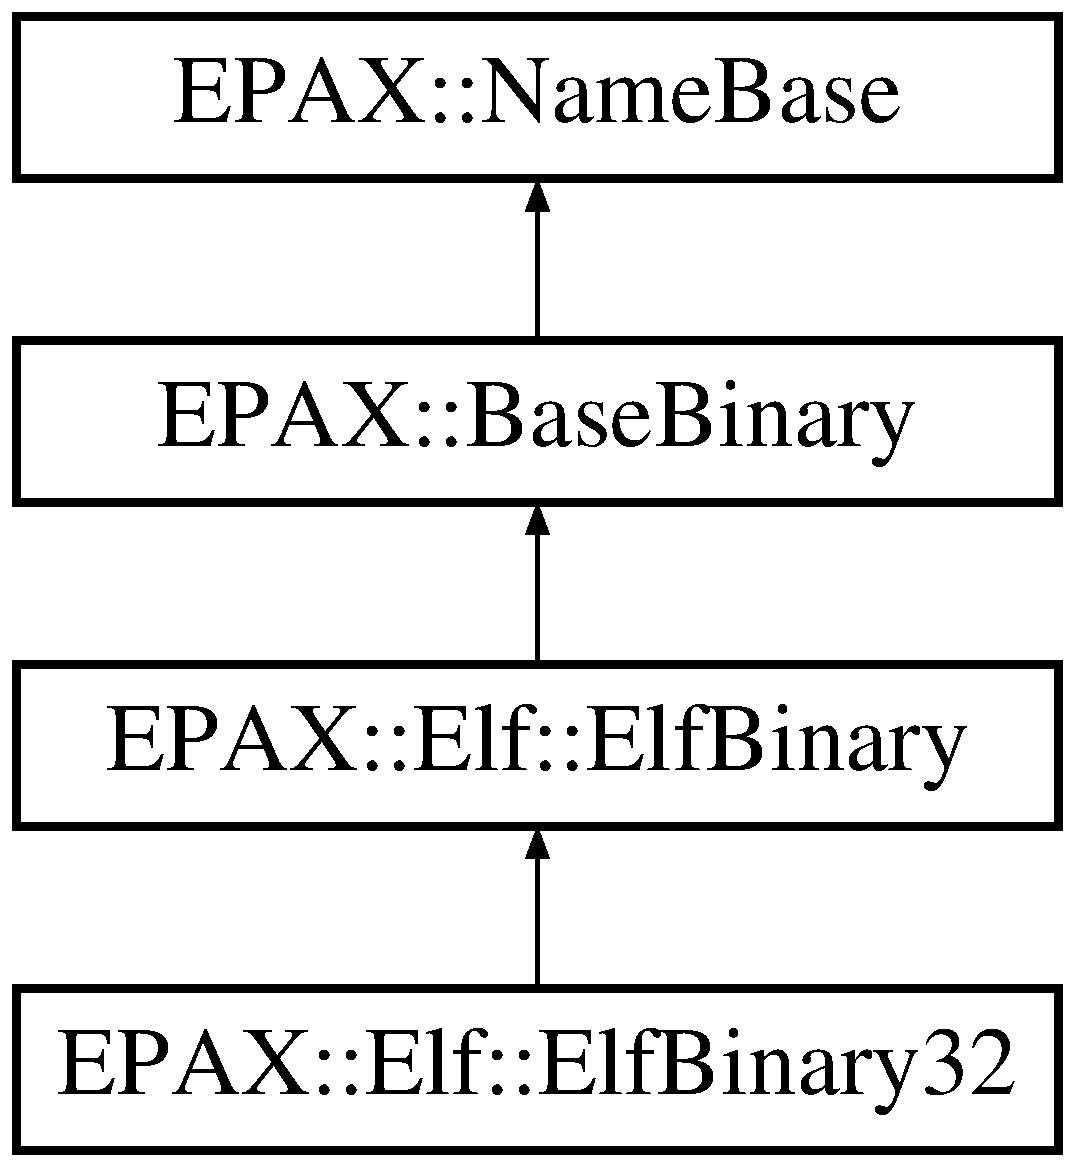
\includegraphics[height=4.000000cm]{class_e_p_a_x_1_1_elf_1_1_elf_binary32}
\end{center}
\end{figure}
\subsection*{\-Public \-Member \-Functions}
\begin{DoxyCompactItemize}
\item 
\hyperlink{class_e_p_a_x_1_1_elf_1_1_elf_binary32_a745eda06077bee1c3968ac6d8185d86e}{\-Elf\-Binary32} (std\-::string n)
\item 
virtual \hyperlink{class_e_p_a_x_1_1_elf_1_1_elf_binary32_a44ba58a5202e5fda219d6008ff90d153}{$\sim$\-Elf\-Binary32} ()
\item 
\hyperlink{namespace_e_p_a_x_a4be639c006ef14def4708b37ee6dd67d}{\-Binary\-Format} \hyperlink{class_e_p_a_x_1_1_elf_1_1_elf_binary32_ad3c232fe03109e9a59e5456420d4fed3}{get\-Format} ()
\end{DoxyCompactItemize}


\subsection{\-Detailed \-Description}


\-Definition at line 84 of file \-Elf\-Binary.\-hpp.



\subsection{\-Constructor \& \-Destructor \-Documentation}
\hypertarget{class_e_p_a_x_1_1_elf_1_1_elf_binary32_a745eda06077bee1c3968ac6d8185d86e}{\index{\-E\-P\-A\-X\-::\-Elf\-::\-Elf\-Binary32@{\-E\-P\-A\-X\-::\-Elf\-::\-Elf\-Binary32}!\-Elf\-Binary32@{\-Elf\-Binary32}}
\index{\-Elf\-Binary32@{\-Elf\-Binary32}!EPAX::Elf::ElfBinary32@{\-E\-P\-A\-X\-::\-Elf\-::\-Elf\-Binary32}}
\subsubsection[{\-Elf\-Binary32}]{\setlength{\rightskip}{0pt plus 5cm}{\bf \-E\-P\-A\-X\-::\-Elf\-::\-Elf\-Binary32\-::\-Elf\-Binary32} (
\begin{DoxyParamCaption}
\item[{std\-::string}]{n}
\end{DoxyParamCaption}
)}}\label{class_e_p_a_x_1_1_elf_1_1_elf_binary32_a745eda06077bee1c3968ac6d8185d86e}


\-Definition at line 124 of file \-Elf\-Binary.\-cpp.

\hypertarget{class_e_p_a_x_1_1_elf_1_1_elf_binary32_a44ba58a5202e5fda219d6008ff90d153}{\index{\-E\-P\-A\-X\-::\-Elf\-::\-Elf\-Binary32@{\-E\-P\-A\-X\-::\-Elf\-::\-Elf\-Binary32}!$\sim$\-Elf\-Binary32@{$\sim$\-Elf\-Binary32}}
\index{$\sim$\-Elf\-Binary32@{$\sim$\-Elf\-Binary32}!EPAX::Elf::ElfBinary32@{\-E\-P\-A\-X\-::\-Elf\-::\-Elf\-Binary32}}
\subsubsection[{$\sim$\-Elf\-Binary32}]{\setlength{\rightskip}{0pt plus 5cm}virtual {\bf \-E\-P\-A\-X\-::\-Elf\-::\-Elf\-Binary32\-::$\sim$\-Elf\-Binary32} (
\begin{DoxyParamCaption}
{}
\end{DoxyParamCaption}
)\hspace{0.3cm}{\ttfamily  \mbox{[}inline, virtual\mbox{]}}}}\label{class_e_p_a_x_1_1_elf_1_1_elf_binary32_a44ba58a5202e5fda219d6008ff90d153}


\-Definition at line 87 of file \-Elf\-Binary.\-hpp.



\subsection{\-Member \-Function \-Documentation}
\hypertarget{class_e_p_a_x_1_1_elf_1_1_elf_binary32_ad3c232fe03109e9a59e5456420d4fed3}{\index{\-E\-P\-A\-X\-::\-Elf\-::\-Elf\-Binary32@{\-E\-P\-A\-X\-::\-Elf\-::\-Elf\-Binary32}!get\-Format@{get\-Format}}
\index{get\-Format@{get\-Format}!EPAX::Elf::ElfBinary32@{\-E\-P\-A\-X\-::\-Elf\-::\-Elf\-Binary32}}
\subsubsection[{get\-Format}]{\setlength{\rightskip}{0pt plus 5cm}{\bf \-Binary\-Format} {\bf \-E\-P\-A\-X\-::\-Elf\-::\-Elf\-Binary32\-::get\-Format} (
\begin{DoxyParamCaption}
{}
\end{DoxyParamCaption}
)\hspace{0.3cm}{\ttfamily  \mbox{[}inline, virtual\mbox{]}}}}\label{class_e_p_a_x_1_1_elf_1_1_elf_binary32_ad3c232fe03109e9a59e5456420d4fed3}


\-Implements \hyperlink{class_e_p_a_x_1_1_elf_1_1_elf_binary_a2f8cfe8d4567e4aefbeb0717da3f0e9c}{\-E\-P\-A\-X\-::\-Elf\-::\-Elf\-Binary}.



\-Definition at line 89 of file \-Elf\-Binary.\-hpp.



\-The documentation for this class was generated from the following files\-:\begin{DoxyCompactItemize}
\item 
\hyperlink{_elf_binary_8hpp}{\-Elf\-Binary.\-hpp}\item 
\hyperlink{_elf_binary_8cpp}{\-Elf\-Binary.\-cpp}\end{DoxyCompactItemize}

\hypertarget{class_e_p_a_x_1_1_elf_1_1_elf_binary64}{\section{\-E\-P\-A\-X\-:\-:\-Elf\-:\-:\-Elf\-Binary64 \-Class \-Reference}
\label{class_e_p_a_x_1_1_elf_1_1_elf_binary64}\index{\-E\-P\-A\-X\-::\-Elf\-::\-Elf\-Binary64@{\-E\-P\-A\-X\-::\-Elf\-::\-Elf\-Binary64}}
}


{\ttfamily \#include $<$\-Elf\-Binary.\-hpp$>$}

\-Inheritance diagram for \-E\-P\-A\-X\-:\-:\-Elf\-:\-:\-Elf\-Binary64\-:\begin{figure}[H]
\begin{center}
\leavevmode
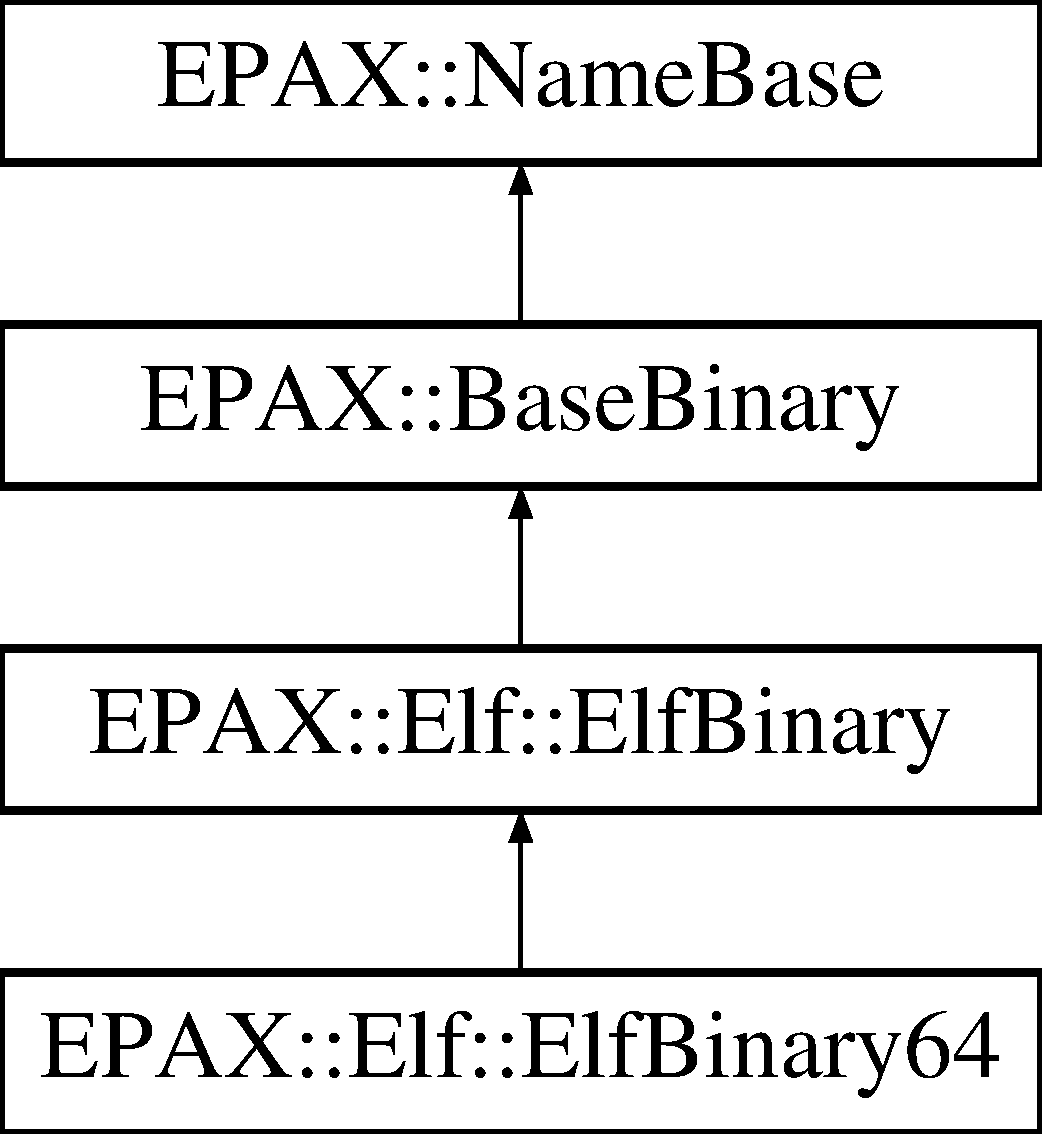
\includegraphics[height=4.000000cm]{class_e_p_a_x_1_1_elf_1_1_elf_binary64}
\end{center}
\end{figure}
\subsection*{\-Public \-Member \-Functions}
\begin{DoxyCompactItemize}
\item 
\hyperlink{class_e_p_a_x_1_1_elf_1_1_elf_binary64_a47d6997a1bbad96ade4b7d73533ffffb}{\-Elf\-Binary64} (std\-::string n)
\item 
virtual \hyperlink{class_e_p_a_x_1_1_elf_1_1_elf_binary64_a31c48ee0193933b69f0af9dacc881b07}{$\sim$\-Elf\-Binary64} ()
\item 
\hyperlink{namespace_e_p_a_x_a4be639c006ef14def4708b37ee6dd67d}{\-Binary\-Format} \hyperlink{class_e_p_a_x_1_1_elf_1_1_elf_binary64_a8d4ac63ef8a488fb6ad98fd24ad36d07}{get\-Format} ()
\end{DoxyCompactItemize}


\subsection{\-Detailed \-Description}


\-Definition at line 92 of file \-Elf\-Binary.\-hpp.



\subsection{\-Constructor \& \-Destructor \-Documentation}
\hypertarget{class_e_p_a_x_1_1_elf_1_1_elf_binary64_a47d6997a1bbad96ade4b7d73533ffffb}{\index{\-E\-P\-A\-X\-::\-Elf\-::\-Elf\-Binary64@{\-E\-P\-A\-X\-::\-Elf\-::\-Elf\-Binary64}!\-Elf\-Binary64@{\-Elf\-Binary64}}
\index{\-Elf\-Binary64@{\-Elf\-Binary64}!EPAX::Elf::ElfBinary64@{\-E\-P\-A\-X\-::\-Elf\-::\-Elf\-Binary64}}
\subsubsection[{\-Elf\-Binary64}]{\setlength{\rightskip}{0pt plus 5cm}{\bf \-E\-P\-A\-X\-::\-Elf\-::\-Elf\-Binary64\-::\-Elf\-Binary64} (
\begin{DoxyParamCaption}
\item[{std\-::string}]{n}
\end{DoxyParamCaption}
)}}\label{class_e_p_a_x_1_1_elf_1_1_elf_binary64_a47d6997a1bbad96ade4b7d73533ffffb}


\-Definition at line 130 of file \-Elf\-Binary.\-cpp.

\hypertarget{class_e_p_a_x_1_1_elf_1_1_elf_binary64_a31c48ee0193933b69f0af9dacc881b07}{\index{\-E\-P\-A\-X\-::\-Elf\-::\-Elf\-Binary64@{\-E\-P\-A\-X\-::\-Elf\-::\-Elf\-Binary64}!$\sim$\-Elf\-Binary64@{$\sim$\-Elf\-Binary64}}
\index{$\sim$\-Elf\-Binary64@{$\sim$\-Elf\-Binary64}!EPAX::Elf::ElfBinary64@{\-E\-P\-A\-X\-::\-Elf\-::\-Elf\-Binary64}}
\subsubsection[{$\sim$\-Elf\-Binary64}]{\setlength{\rightskip}{0pt plus 5cm}virtual {\bf \-E\-P\-A\-X\-::\-Elf\-::\-Elf\-Binary64\-::$\sim$\-Elf\-Binary64} (
\begin{DoxyParamCaption}
{}
\end{DoxyParamCaption}
)\hspace{0.3cm}{\ttfamily  \mbox{[}inline, virtual\mbox{]}}}}\label{class_e_p_a_x_1_1_elf_1_1_elf_binary64_a31c48ee0193933b69f0af9dacc881b07}


\-Definition at line 95 of file \-Elf\-Binary.\-hpp.



\subsection{\-Member \-Function \-Documentation}
\hypertarget{class_e_p_a_x_1_1_elf_1_1_elf_binary64_a8d4ac63ef8a488fb6ad98fd24ad36d07}{\index{\-E\-P\-A\-X\-::\-Elf\-::\-Elf\-Binary64@{\-E\-P\-A\-X\-::\-Elf\-::\-Elf\-Binary64}!get\-Format@{get\-Format}}
\index{get\-Format@{get\-Format}!EPAX::Elf::ElfBinary64@{\-E\-P\-A\-X\-::\-Elf\-::\-Elf\-Binary64}}
\subsubsection[{get\-Format}]{\setlength{\rightskip}{0pt plus 5cm}{\bf \-Binary\-Format} {\bf \-E\-P\-A\-X\-::\-Elf\-::\-Elf\-Binary64\-::get\-Format} (
\begin{DoxyParamCaption}
{}
\end{DoxyParamCaption}
)\hspace{0.3cm}{\ttfamily  \mbox{[}inline, virtual\mbox{]}}}}\label{class_e_p_a_x_1_1_elf_1_1_elf_binary64_a8d4ac63ef8a488fb6ad98fd24ad36d07}


\-Implements \hyperlink{class_e_p_a_x_1_1_elf_1_1_elf_binary_a2f8cfe8d4567e4aefbeb0717da3f0e9c}{\-E\-P\-A\-X\-::\-Elf\-::\-Elf\-Binary}.



\-Definition at line 97 of file \-Elf\-Binary.\-hpp.



\-The documentation for this class was generated from the following files\-:\begin{DoxyCompactItemize}
\item 
\hyperlink{_elf_binary_8hpp}{\-Elf\-Binary.\-hpp}\item 
\hyperlink{_elf_binary_8cpp}{\-Elf\-Binary.\-cpp}\end{DoxyCompactItemize}

\hypertarget{class_e_p_a_x_1_1_elf_1_1_elf_string_table}{\section{\-E\-P\-A\-X\-:\-:\-Elf\-:\-:\-Elf\-String\-Table \-Class \-Reference}
\label{class_e_p_a_x_1_1_elf_1_1_elf_string_table}\index{\-E\-P\-A\-X\-::\-Elf\-::\-Elf\-String\-Table@{\-E\-P\-A\-X\-::\-Elf\-::\-Elf\-String\-Table}}
}


{\ttfamily \#include $<$\-Elf\-Binary.\-hpp$>$}

\-Inheritance diagram for \-E\-P\-A\-X\-:\-:\-Elf\-:\-:\-Elf\-String\-Table\-:\begin{figure}[H]
\begin{center}
\leavevmode
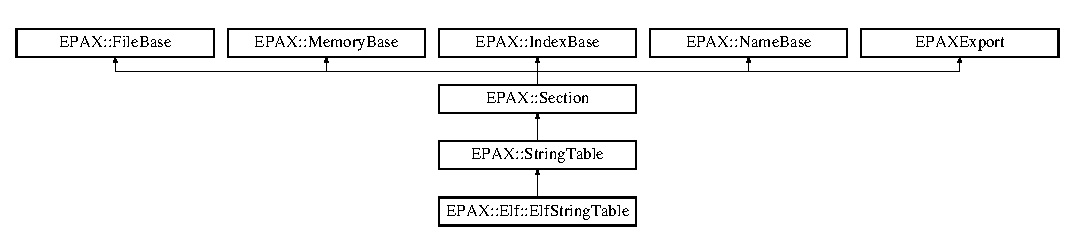
\includegraphics[height=2.800000cm]{class_e_p_a_x_1_1_elf_1_1_elf_string_table}
\end{center}
\end{figure}
\subsection*{\-Public \-Member \-Functions}
\begin{DoxyCompactItemize}
\item 
\hyperlink{class_e_p_a_x_1_1_elf_1_1_elf_string_table_a24ad50d1642c3c432e3623c0b633f59d}{\-Elf\-String\-Table} (\hyperlink{class_e_p_a_x_1_1_base_binary}{\-Base\-Binary} $\ast$b, uint64\-\_\-t o, uint64\-\_\-t fs, uint64\-\_\-t ma, uint64\-\_\-t ms, uint32\-\_\-t i, std\-::string n)
\item 
\hyperlink{class_e_p_a_x_1_1_elf_1_1_elf_string_table_a7eb7c7cf0000dbc952084bf544cef094}{$\sim$\-Elf\-String\-Table} ()
\item 
char $\ast$ \hyperlink{class_e_p_a_x_1_1_elf_1_1_elf_string_table_a5090981e577dceb27e8dd6c63f1992ba}{get\-String\-At} (uint32\-\_\-t i)
\item 
void \hyperlink{class_e_p_a_x_1_1_elf_1_1_elf_string_table_a025f9dab1825e838634d998481bfa1cf}{print} (std\-::ostream \&stream=std\-::cout)
\end{DoxyCompactItemize}


\subsection{\-Detailed \-Description}


\-Definition at line 223 of file \-Elf\-Binary.\-hpp.



\subsection{\-Constructor \& \-Destructor \-Documentation}
\hypertarget{class_e_p_a_x_1_1_elf_1_1_elf_string_table_a24ad50d1642c3c432e3623c0b633f59d}{\index{\-E\-P\-A\-X\-::\-Elf\-::\-Elf\-String\-Table@{\-E\-P\-A\-X\-::\-Elf\-::\-Elf\-String\-Table}!\-Elf\-String\-Table@{\-Elf\-String\-Table}}
\index{\-Elf\-String\-Table@{\-Elf\-String\-Table}!EPAX::Elf::ElfStringTable@{\-E\-P\-A\-X\-::\-Elf\-::\-Elf\-String\-Table}}
\subsubsection[{\-Elf\-String\-Table}]{\setlength{\rightskip}{0pt plus 5cm}{\bf \-E\-P\-A\-X\-::\-Elf\-::\-Elf\-String\-Table\-::\-Elf\-String\-Table} (
\begin{DoxyParamCaption}
\item[{{\bf \-Base\-Binary} $\ast$}]{b, }
\item[{uint64\-\_\-t}]{o, }
\item[{uint64\-\_\-t}]{fs, }
\item[{uint64\-\_\-t}]{ma, }
\item[{uint64\-\_\-t}]{ms, }
\item[{uint32\-\_\-t}]{i, }
\item[{std\-::string}]{n}
\end{DoxyParamCaption}
)}}\label{class_e_p_a_x_1_1_elf_1_1_elf_string_table_a24ad50d1642c3c432e3623c0b633f59d}


\-Definition at line 629 of file \-Elf\-Binary.\-cpp.

\hypertarget{class_e_p_a_x_1_1_elf_1_1_elf_string_table_a7eb7c7cf0000dbc952084bf544cef094}{\index{\-E\-P\-A\-X\-::\-Elf\-::\-Elf\-String\-Table@{\-E\-P\-A\-X\-::\-Elf\-::\-Elf\-String\-Table}!$\sim$\-Elf\-String\-Table@{$\sim$\-Elf\-String\-Table}}
\index{$\sim$\-Elf\-String\-Table@{$\sim$\-Elf\-String\-Table}!EPAX::Elf::ElfStringTable@{\-E\-P\-A\-X\-::\-Elf\-::\-Elf\-String\-Table}}
\subsubsection[{$\sim$\-Elf\-String\-Table}]{\setlength{\rightskip}{0pt plus 5cm}{\bf \-E\-P\-A\-X\-::\-Elf\-::\-Elf\-String\-Table\-::$\sim$\-Elf\-String\-Table} (
\begin{DoxyParamCaption}
{}
\end{DoxyParamCaption}
)}}\label{class_e_p_a_x_1_1_elf_1_1_elf_string_table_a7eb7c7cf0000dbc952084bf544cef094}


\-Definition at line 638 of file \-Elf\-Binary.\-cpp.



\subsection{\-Member \-Function \-Documentation}
\hypertarget{class_e_p_a_x_1_1_elf_1_1_elf_string_table_a5090981e577dceb27e8dd6c63f1992ba}{\index{\-E\-P\-A\-X\-::\-Elf\-::\-Elf\-String\-Table@{\-E\-P\-A\-X\-::\-Elf\-::\-Elf\-String\-Table}!get\-String\-At@{get\-String\-At}}
\index{get\-String\-At@{get\-String\-At}!EPAX::Elf::ElfStringTable@{\-E\-P\-A\-X\-::\-Elf\-::\-Elf\-String\-Table}}
\subsubsection[{get\-String\-At}]{\setlength{\rightskip}{0pt plus 5cm}char $\ast$ {\bf \-E\-P\-A\-X\-::\-Elf\-::\-Elf\-String\-Table\-::get\-String\-At} (
\begin{DoxyParamCaption}
\item[{uint32\-\_\-t}]{i}
\end{DoxyParamCaption}
)\hspace{0.3cm}{\ttfamily  \mbox{[}virtual\mbox{]}}}}\label{class_e_p_a_x_1_1_elf_1_1_elf_string_table_a5090981e577dceb27e8dd6c63f1992ba}


\-Implements \hyperlink{class_e_p_a_x_1_1_string_table_a1931cd14e2e3e1be340386f8bbbc6d2a}{\-E\-P\-A\-X\-::\-String\-Table}.



\-Definition at line 644 of file \-Elf\-Binary.\-cpp.

\hypertarget{class_e_p_a_x_1_1_elf_1_1_elf_string_table_a025f9dab1825e838634d998481bfa1cf}{\index{\-E\-P\-A\-X\-::\-Elf\-::\-Elf\-String\-Table@{\-E\-P\-A\-X\-::\-Elf\-::\-Elf\-String\-Table}!print@{print}}
\index{print@{print}!EPAX::Elf::ElfStringTable@{\-E\-P\-A\-X\-::\-Elf\-::\-Elf\-String\-Table}}
\subsubsection[{print}]{\setlength{\rightskip}{0pt plus 5cm}void {\bf \-E\-P\-A\-X\-::\-Elf\-::\-Elf\-String\-Table\-::print} (
\begin{DoxyParamCaption}
\item[{std\-::ostream \&}]{stream = {\ttfamily std\-:\-:cout}}
\end{DoxyParamCaption}
)\hspace{0.3cm}{\ttfamily  \mbox{[}virtual\mbox{]}}}}\label{class_e_p_a_x_1_1_elf_1_1_elf_string_table_a025f9dab1825e838634d998481bfa1cf}


\-Reimplemented from \hyperlink{class_e_p_a_x_1_1_section_ad79a91be22efd4499b78d2554ebc8285}{\-E\-P\-A\-X\-::\-Section}.



\-Definition at line 508 of file \-Elf\-Binary.\-cpp.



\-The documentation for this class was generated from the following files\-:\begin{DoxyCompactItemize}
\item 
\hyperlink{_elf_binary_8hpp}{\-Elf\-Binary.\-hpp}\item 
\hyperlink{_elf_binary_8cpp}{\-Elf\-Binary.\-cpp}\end{DoxyCompactItemize}

\hypertarget{class_e_p_a_x_1_1_elf_1_1_elf_symbol}{\section{\-E\-P\-A\-X\-:\-:\-Elf\-:\-:\-Elf\-Symbol \-Class \-Reference}
\label{class_e_p_a_x_1_1_elf_1_1_elf_symbol}\index{\-E\-P\-A\-X\-::\-Elf\-::\-Elf\-Symbol@{\-E\-P\-A\-X\-::\-Elf\-::\-Elf\-Symbol}}
}


{\ttfamily \#include $<$\-Elf\-Binary.\-hpp$>$}

\-Inheritance diagram for \-E\-P\-A\-X\-:\-:\-Elf\-:\-:\-Elf\-Symbol\-:\begin{figure}[H]
\begin{center}
\leavevmode
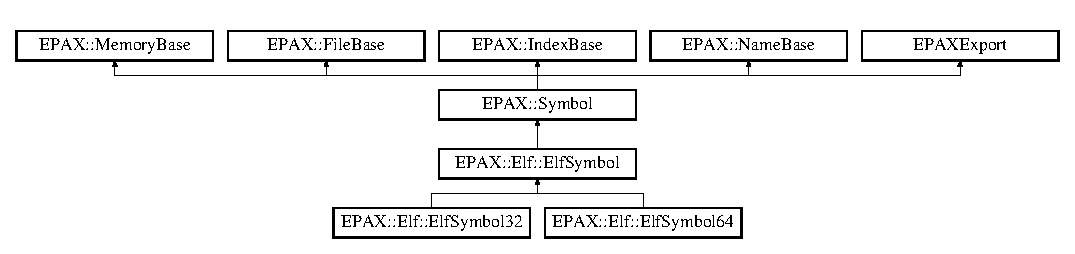
\includegraphics[height=2.966887cm]{class_e_p_a_x_1_1_elf_1_1_elf_symbol}
\end{center}
\end{figure}
\subsection*{\-Public \-Member \-Functions}
\begin{DoxyCompactItemize}
\item 
\hyperlink{class_e_p_a_x_1_1_elf_1_1_elf_symbol_a3907cf60c70f5abf4c5c9522c7f63a74}{\-Elf\-Symbol} (\hyperlink{class_e_p_a_x_1_1_base_binary}{\-Base\-Binary} $\ast$b, uint64\-\_\-t o, uint64\-\_\-t s, uint32\-\_\-t i)
\item 
virtual \hyperlink{class_e_p_a_x_1_1_elf_1_1_elf_symbol_af409dbd1b83de98f977c7d8eea73e66f}{$\sim$\-Elf\-Symbol} ()
\item 
void \hyperlink{class_e_p_a_x_1_1_elf_1_1_elf_symbol_a19338c302c20a71a101be47205a44908}{print} (std\-::ostream \&stream=std\-::cout)
\item 
virtual uint64\-\_\-t \hyperlink{class_e_p_a_x_1_1_elf_1_1_elf_symbol_a84ccb1d566bee093da094e2c4b617ba7}{get\-Name\-Index} ()=0
\item 
virtual uint64\-\_\-t \hyperlink{class_e_p_a_x_1_1_elf_1_1_elf_symbol_a20b9df356b7d4ef1481dc8fdeaf4b2fc}{get\-Value} ()=0
\item 
virtual uint32\-\_\-t \hyperlink{class_e_p_a_x_1_1_elf_1_1_elf_symbol_a92184692a8f808802963e1a7ca9606d7}{get\-Section} ()=0
\item 
virtual uint32\-\_\-t \hyperlink{class_e_p_a_x_1_1_elf_1_1_elf_symbol_a38fb6985ad991affbb10051eac2aa75e}{get\-Size} ()=0
\item 
virtual uint32\-\_\-t \hyperlink{class_e_p_a_x_1_1_elf_1_1_elf_symbol_a540aabaf19398d8512f7bdb9255fa9d6}{get\-Type} ()=0
\item 
virtual uint32\-\_\-t \hyperlink{class_e_p_a_x_1_1_elf_1_1_elf_symbol_a3bed4c1dcd7d20cdd492c16977e59b93}{get\-Binding} ()=0
\item 
virtual uint64\-\_\-t \hyperlink{class_e_p_a_x_1_1_elf_1_1_elf_symbol_a31b56e39f50f311ab23e878faba5d5b4}{get\-Visibility} ()=0
\item 
bool \hyperlink{class_e_p_a_x_1_1_elf_1_1_elf_symbol_ad6142f5f07372bffd2f0b9a482696821}{is\-Function} ()
\item 
bool \hyperlink{class_e_p_a_x_1_1_elf_1_1_elf_symbol_a4f27b2be55f35a4c9a75b5e52bce6e23}{is\-Thumb\-Function} ()
\item 
uint64\-\_\-t \hyperlink{class_e_p_a_x_1_1_elf_1_1_elf_symbol_a81a2839b65f94ce09a1f65a70bb268e1}{get\-Function\-Address} ()
\end{DoxyCompactItemize}
\subsection*{\-Protected \-Attributes}
\begin{DoxyCompactItemize}
\item 
\hyperlink{_e_p_a_x_common_internal_8hpp_a17755bdd71c02e656c667b16de61dd7b}{rawbyte\-\_\-t} $\ast$ \hyperlink{class_e_p_a_x_1_1_elf_1_1_elf_symbol_a3c57705558738ca7aa9803260ff9da9e}{entry}
\end{DoxyCompactItemize}


\subsection{\-Detailed \-Description}


\-Definition at line 170 of file \-Elf\-Binary.\-hpp.



\subsection{\-Constructor \& \-Destructor \-Documentation}
\hypertarget{class_e_p_a_x_1_1_elf_1_1_elf_symbol_a3907cf60c70f5abf4c5c9522c7f63a74}{\index{\-E\-P\-A\-X\-::\-Elf\-::\-Elf\-Symbol@{\-E\-P\-A\-X\-::\-Elf\-::\-Elf\-Symbol}!\-Elf\-Symbol@{\-Elf\-Symbol}}
\index{\-Elf\-Symbol@{\-Elf\-Symbol}!EPAX::Elf::ElfSymbol@{\-E\-P\-A\-X\-::\-Elf\-::\-Elf\-Symbol}}
\subsubsection[{\-Elf\-Symbol}]{\setlength{\rightskip}{0pt plus 5cm}{\bf \-E\-P\-A\-X\-::\-Elf\-::\-Elf\-Symbol\-::\-Elf\-Symbol} (
\begin{DoxyParamCaption}
\item[{{\bf \-Base\-Binary} $\ast$}]{b, }
\item[{uint64\-\_\-t}]{o, }
\item[{uint64\-\_\-t}]{s, }
\item[{uint32\-\_\-t}]{i}
\end{DoxyParamCaption}
)}}\label{class_e_p_a_x_1_1_elf_1_1_elf_symbol_a3907cf60c70f5abf4c5c9522c7f63a74}


\-Definition at line 496 of file \-Elf\-Binary.\-cpp.

\hypertarget{class_e_p_a_x_1_1_elf_1_1_elf_symbol_af409dbd1b83de98f977c7d8eea73e66f}{\index{\-E\-P\-A\-X\-::\-Elf\-::\-Elf\-Symbol@{\-E\-P\-A\-X\-::\-Elf\-::\-Elf\-Symbol}!$\sim$\-Elf\-Symbol@{$\sim$\-Elf\-Symbol}}
\index{$\sim$\-Elf\-Symbol@{$\sim$\-Elf\-Symbol}!EPAX::Elf::ElfSymbol@{\-E\-P\-A\-X\-::\-Elf\-::\-Elf\-Symbol}}
\subsubsection[{$\sim$\-Elf\-Symbol}]{\setlength{\rightskip}{0pt plus 5cm}{\bf \-E\-P\-A\-X\-::\-Elf\-::\-Elf\-Symbol\-::$\sim$\-Elf\-Symbol} (
\begin{DoxyParamCaption}
{}
\end{DoxyParamCaption}
)\hspace{0.3cm}{\ttfamily  \mbox{[}virtual\mbox{]}}}}\label{class_e_p_a_x_1_1_elf_1_1_elf_symbol_af409dbd1b83de98f977c7d8eea73e66f}


\-Definition at line 502 of file \-Elf\-Binary.\-cpp.



\subsection{\-Member \-Function \-Documentation}
\hypertarget{class_e_p_a_x_1_1_elf_1_1_elf_symbol_a3bed4c1dcd7d20cdd492c16977e59b93}{\index{\-E\-P\-A\-X\-::\-Elf\-::\-Elf\-Symbol@{\-E\-P\-A\-X\-::\-Elf\-::\-Elf\-Symbol}!get\-Binding@{get\-Binding}}
\index{get\-Binding@{get\-Binding}!EPAX::Elf::ElfSymbol@{\-E\-P\-A\-X\-::\-Elf\-::\-Elf\-Symbol}}
\subsubsection[{get\-Binding}]{\setlength{\rightskip}{0pt plus 5cm}virtual uint32\-\_\-t {\bf \-E\-P\-A\-X\-::\-Elf\-::\-Elf\-Symbol\-::get\-Binding} (
\begin{DoxyParamCaption}
{}
\end{DoxyParamCaption}
)\hspace{0.3cm}{\ttfamily  \mbox{[}pure virtual\mbox{]}}}}\label{class_e_p_a_x_1_1_elf_1_1_elf_symbol_a3bed4c1dcd7d20cdd492c16977e59b93}


\-Implemented in \hyperlink{class_e_p_a_x_1_1_elf_1_1_elf_symbol64_a341e642319d9b9f70ee9dfebdcad4f5b}{\-E\-P\-A\-X\-::\-Elf\-::\-Elf\-Symbol64}, and \hyperlink{class_e_p_a_x_1_1_elf_1_1_elf_symbol32_a9361f33bf04cbfd6623392f1905aaef6}{\-E\-P\-A\-X\-::\-Elf\-::\-Elf\-Symbol32}.

\hypertarget{class_e_p_a_x_1_1_elf_1_1_elf_symbol_a81a2839b65f94ce09a1f65a70bb268e1}{\index{\-E\-P\-A\-X\-::\-Elf\-::\-Elf\-Symbol@{\-E\-P\-A\-X\-::\-Elf\-::\-Elf\-Symbol}!get\-Function\-Address@{get\-Function\-Address}}
\index{get\-Function\-Address@{get\-Function\-Address}!EPAX::Elf::ElfSymbol@{\-E\-P\-A\-X\-::\-Elf\-::\-Elf\-Symbol}}
\subsubsection[{get\-Function\-Address}]{\setlength{\rightskip}{0pt plus 5cm}uint64\-\_\-t {\bf \-E\-P\-A\-X\-::\-Elf\-::\-Elf\-Symbol\-::get\-Function\-Address} (
\begin{DoxyParamCaption}
{}
\end{DoxyParamCaption}
)}}\label{class_e_p_a_x_1_1_elf_1_1_elf_symbol_a81a2839b65f94ce09a1f65a70bb268e1}


\-Definition at line 620 of file \-Elf\-Binary.\-cpp.

\hypertarget{class_e_p_a_x_1_1_elf_1_1_elf_symbol_a84ccb1d566bee093da094e2c4b617ba7}{\index{\-E\-P\-A\-X\-::\-Elf\-::\-Elf\-Symbol@{\-E\-P\-A\-X\-::\-Elf\-::\-Elf\-Symbol}!get\-Name\-Index@{get\-Name\-Index}}
\index{get\-Name\-Index@{get\-Name\-Index}!EPAX::Elf::ElfSymbol@{\-E\-P\-A\-X\-::\-Elf\-::\-Elf\-Symbol}}
\subsubsection[{get\-Name\-Index}]{\setlength{\rightskip}{0pt plus 5cm}virtual uint64\-\_\-t {\bf \-E\-P\-A\-X\-::\-Elf\-::\-Elf\-Symbol\-::get\-Name\-Index} (
\begin{DoxyParamCaption}
{}
\end{DoxyParamCaption}
)\hspace{0.3cm}{\ttfamily  \mbox{[}pure virtual\mbox{]}}}}\label{class_e_p_a_x_1_1_elf_1_1_elf_symbol_a84ccb1d566bee093da094e2c4b617ba7}


\-Implemented in \hyperlink{class_e_p_a_x_1_1_elf_1_1_elf_symbol64_a6e8651a83dfdd485e87e013b4a4790e2}{\-E\-P\-A\-X\-::\-Elf\-::\-Elf\-Symbol64}, and \hyperlink{class_e_p_a_x_1_1_elf_1_1_elf_symbol32_a319c4e22fbb4b99667707a8b0d9412d1}{\-E\-P\-A\-X\-::\-Elf\-::\-Elf\-Symbol32}.

\hypertarget{class_e_p_a_x_1_1_elf_1_1_elf_symbol_a92184692a8f808802963e1a7ca9606d7}{\index{\-E\-P\-A\-X\-::\-Elf\-::\-Elf\-Symbol@{\-E\-P\-A\-X\-::\-Elf\-::\-Elf\-Symbol}!get\-Section@{get\-Section}}
\index{get\-Section@{get\-Section}!EPAX::Elf::ElfSymbol@{\-E\-P\-A\-X\-::\-Elf\-::\-Elf\-Symbol}}
\subsubsection[{get\-Section}]{\setlength{\rightskip}{0pt plus 5cm}virtual uint32\-\_\-t {\bf \-E\-P\-A\-X\-::\-Elf\-::\-Elf\-Symbol\-::get\-Section} (
\begin{DoxyParamCaption}
{}
\end{DoxyParamCaption}
)\hspace{0.3cm}{\ttfamily  \mbox{[}pure virtual\mbox{]}}}}\label{class_e_p_a_x_1_1_elf_1_1_elf_symbol_a92184692a8f808802963e1a7ca9606d7}


\-Implemented in \hyperlink{class_e_p_a_x_1_1_elf_1_1_elf_symbol64_ad2acb7dbbf88685b5bfcfbed2ac1dba4}{\-E\-P\-A\-X\-::\-Elf\-::\-Elf\-Symbol64}, and \hyperlink{class_e_p_a_x_1_1_elf_1_1_elf_symbol32_a5ae0934c001dc2a81dbd88fb1d0ad786}{\-E\-P\-A\-X\-::\-Elf\-::\-Elf\-Symbol32}.

\hypertarget{class_e_p_a_x_1_1_elf_1_1_elf_symbol_a38fb6985ad991affbb10051eac2aa75e}{\index{\-E\-P\-A\-X\-::\-Elf\-::\-Elf\-Symbol@{\-E\-P\-A\-X\-::\-Elf\-::\-Elf\-Symbol}!get\-Size@{get\-Size}}
\index{get\-Size@{get\-Size}!EPAX::Elf::ElfSymbol@{\-E\-P\-A\-X\-::\-Elf\-::\-Elf\-Symbol}}
\subsubsection[{get\-Size}]{\setlength{\rightskip}{0pt plus 5cm}virtual uint32\-\_\-t {\bf \-E\-P\-A\-X\-::\-Elf\-::\-Elf\-Symbol\-::get\-Size} (
\begin{DoxyParamCaption}
{}
\end{DoxyParamCaption}
)\hspace{0.3cm}{\ttfamily  \mbox{[}pure virtual\mbox{]}}}}\label{class_e_p_a_x_1_1_elf_1_1_elf_symbol_a38fb6985ad991affbb10051eac2aa75e}


\-Implemented in \hyperlink{class_e_p_a_x_1_1_elf_1_1_elf_symbol64_a26225a3989efc89a50fa934c53f47276}{\-E\-P\-A\-X\-::\-Elf\-::\-Elf\-Symbol64}, and \hyperlink{class_e_p_a_x_1_1_elf_1_1_elf_symbol32_ae5ef1d81c0a3d126441e147104f8ea85}{\-E\-P\-A\-X\-::\-Elf\-::\-Elf\-Symbol32}.

\hypertarget{class_e_p_a_x_1_1_elf_1_1_elf_symbol_a540aabaf19398d8512f7bdb9255fa9d6}{\index{\-E\-P\-A\-X\-::\-Elf\-::\-Elf\-Symbol@{\-E\-P\-A\-X\-::\-Elf\-::\-Elf\-Symbol}!get\-Type@{get\-Type}}
\index{get\-Type@{get\-Type}!EPAX::Elf::ElfSymbol@{\-E\-P\-A\-X\-::\-Elf\-::\-Elf\-Symbol}}
\subsubsection[{get\-Type}]{\setlength{\rightskip}{0pt plus 5cm}virtual uint32\-\_\-t {\bf \-E\-P\-A\-X\-::\-Elf\-::\-Elf\-Symbol\-::get\-Type} (
\begin{DoxyParamCaption}
{}
\end{DoxyParamCaption}
)\hspace{0.3cm}{\ttfamily  \mbox{[}pure virtual\mbox{]}}}}\label{class_e_p_a_x_1_1_elf_1_1_elf_symbol_a540aabaf19398d8512f7bdb9255fa9d6}


\-Implemented in \hyperlink{class_e_p_a_x_1_1_elf_1_1_elf_symbol64_a397faa7562b27ba2d543328a69e17077}{\-E\-P\-A\-X\-::\-Elf\-::\-Elf\-Symbol64}, and \hyperlink{class_e_p_a_x_1_1_elf_1_1_elf_symbol32_a870365328bf8943618c3a3f907f26b24}{\-E\-P\-A\-X\-::\-Elf\-::\-Elf\-Symbol32}.

\hypertarget{class_e_p_a_x_1_1_elf_1_1_elf_symbol_a20b9df356b7d4ef1481dc8fdeaf4b2fc}{\index{\-E\-P\-A\-X\-::\-Elf\-::\-Elf\-Symbol@{\-E\-P\-A\-X\-::\-Elf\-::\-Elf\-Symbol}!get\-Value@{get\-Value}}
\index{get\-Value@{get\-Value}!EPAX::Elf::ElfSymbol@{\-E\-P\-A\-X\-::\-Elf\-::\-Elf\-Symbol}}
\subsubsection[{get\-Value}]{\setlength{\rightskip}{0pt plus 5cm}virtual uint64\-\_\-t {\bf \-E\-P\-A\-X\-::\-Elf\-::\-Elf\-Symbol\-::get\-Value} (
\begin{DoxyParamCaption}
{}
\end{DoxyParamCaption}
)\hspace{0.3cm}{\ttfamily  \mbox{[}pure virtual\mbox{]}}}}\label{class_e_p_a_x_1_1_elf_1_1_elf_symbol_a20b9df356b7d4ef1481dc8fdeaf4b2fc}


\-Implemented in \hyperlink{class_e_p_a_x_1_1_elf_1_1_elf_symbol64_a47e49dde9967bc7cf3f8caeb3b1880fd}{\-E\-P\-A\-X\-::\-Elf\-::\-Elf\-Symbol64}, and \hyperlink{class_e_p_a_x_1_1_elf_1_1_elf_symbol32_a2b4bb23d3d59280ccbbdf0b239bc4ce2}{\-E\-P\-A\-X\-::\-Elf\-::\-Elf\-Symbol32}.

\hypertarget{class_e_p_a_x_1_1_elf_1_1_elf_symbol_a31b56e39f50f311ab23e878faba5d5b4}{\index{\-E\-P\-A\-X\-::\-Elf\-::\-Elf\-Symbol@{\-E\-P\-A\-X\-::\-Elf\-::\-Elf\-Symbol}!get\-Visibility@{get\-Visibility}}
\index{get\-Visibility@{get\-Visibility}!EPAX::Elf::ElfSymbol@{\-E\-P\-A\-X\-::\-Elf\-::\-Elf\-Symbol}}
\subsubsection[{get\-Visibility}]{\setlength{\rightskip}{0pt plus 5cm}virtual uint64\-\_\-t {\bf \-E\-P\-A\-X\-::\-Elf\-::\-Elf\-Symbol\-::get\-Visibility} (
\begin{DoxyParamCaption}
{}
\end{DoxyParamCaption}
)\hspace{0.3cm}{\ttfamily  \mbox{[}pure virtual\mbox{]}}}}\label{class_e_p_a_x_1_1_elf_1_1_elf_symbol_a31b56e39f50f311ab23e878faba5d5b4}


\-Implemented in \hyperlink{class_e_p_a_x_1_1_elf_1_1_elf_symbol64_a0df4c678ba3e7c3e756c6a81152244fa}{\-E\-P\-A\-X\-::\-Elf\-::\-Elf\-Symbol64}, and \hyperlink{class_e_p_a_x_1_1_elf_1_1_elf_symbol32_a547bb437518ff680a5b35c36ebc5e39a}{\-E\-P\-A\-X\-::\-Elf\-::\-Elf\-Symbol32}.

\hypertarget{class_e_p_a_x_1_1_elf_1_1_elf_symbol_ad6142f5f07372bffd2f0b9a482696821}{\index{\-E\-P\-A\-X\-::\-Elf\-::\-Elf\-Symbol@{\-E\-P\-A\-X\-::\-Elf\-::\-Elf\-Symbol}!is\-Function@{is\-Function}}
\index{is\-Function@{is\-Function}!EPAX::Elf::ElfSymbol@{\-E\-P\-A\-X\-::\-Elf\-::\-Elf\-Symbol}}
\subsubsection[{is\-Function}]{\setlength{\rightskip}{0pt plus 5cm}bool {\bf \-E\-P\-A\-X\-::\-Elf\-::\-Elf\-Symbol\-::is\-Function} (
\begin{DoxyParamCaption}
{}
\end{DoxyParamCaption}
)\hspace{0.3cm}{\ttfamily  \mbox{[}virtual\mbox{]}}}}\label{class_e_p_a_x_1_1_elf_1_1_elf_symbol_ad6142f5f07372bffd2f0b9a482696821}


\-Implements \hyperlink{class_e_p_a_x_1_1_symbol_a1dc3c27cb8debeda55cad9d3e04a7be5}{\-E\-P\-A\-X\-::\-Symbol}.



\-Definition at line 612 of file \-Elf\-Binary.\-cpp.

\hypertarget{class_e_p_a_x_1_1_elf_1_1_elf_symbol_a4f27b2be55f35a4c9a75b5e52bce6e23}{\index{\-E\-P\-A\-X\-::\-Elf\-::\-Elf\-Symbol@{\-E\-P\-A\-X\-::\-Elf\-::\-Elf\-Symbol}!is\-Thumb\-Function@{is\-Thumb\-Function}}
\index{is\-Thumb\-Function@{is\-Thumb\-Function}!EPAX::Elf::ElfSymbol@{\-E\-P\-A\-X\-::\-Elf\-::\-Elf\-Symbol}}
\subsubsection[{is\-Thumb\-Function}]{\setlength{\rightskip}{0pt plus 5cm}bool {\bf \-E\-P\-A\-X\-::\-Elf\-::\-Elf\-Symbol\-::is\-Thumb\-Function} (
\begin{DoxyParamCaption}
{}
\end{DoxyParamCaption}
)\hspace{0.3cm}{\ttfamily  \mbox{[}virtual\mbox{]}}}}\label{class_e_p_a_x_1_1_elf_1_1_elf_symbol_a4f27b2be55f35a4c9a75b5e52bce6e23}


\-Implements \hyperlink{class_e_p_a_x_1_1_symbol_a58d8007f908063fc4602c042a739bd8f}{\-E\-P\-A\-X\-::\-Symbol}.



\-Definition at line 616 of file \-Elf\-Binary.\-cpp.

\hypertarget{class_e_p_a_x_1_1_elf_1_1_elf_symbol_a19338c302c20a71a101be47205a44908}{\index{\-E\-P\-A\-X\-::\-Elf\-::\-Elf\-Symbol@{\-E\-P\-A\-X\-::\-Elf\-::\-Elf\-Symbol}!print@{print}}
\index{print@{print}!EPAX::Elf::ElfSymbol@{\-E\-P\-A\-X\-::\-Elf\-::\-Elf\-Symbol}}
\subsubsection[{print}]{\setlength{\rightskip}{0pt plus 5cm}void {\bf \-E\-P\-A\-X\-::\-Elf\-::\-Elf\-Symbol\-::print} (
\begin{DoxyParamCaption}
\item[{std\-::ostream \&}]{stream = {\ttfamily std\-:\-:cout}}
\end{DoxyParamCaption}
)}}\label{class_e_p_a_x_1_1_elf_1_1_elf_symbol_a19338c302c20a71a101be47205a44908}


\-Definition at line 526 of file \-Elf\-Binary.\-cpp.



\subsection{\-Member \-Data \-Documentation}
\hypertarget{class_e_p_a_x_1_1_elf_1_1_elf_symbol_a3c57705558738ca7aa9803260ff9da9e}{\index{\-E\-P\-A\-X\-::\-Elf\-::\-Elf\-Symbol@{\-E\-P\-A\-X\-::\-Elf\-::\-Elf\-Symbol}!entry@{entry}}
\index{entry@{entry}!EPAX::Elf::ElfSymbol@{\-E\-P\-A\-X\-::\-Elf\-::\-Elf\-Symbol}}
\subsubsection[{entry}]{\setlength{\rightskip}{0pt plus 5cm}{\bf rawbyte\-\_\-t}$\ast$ {\bf \-E\-P\-A\-X\-::\-Elf\-::\-Elf\-Symbol\-::entry}\hspace{0.3cm}{\ttfamily  \mbox{[}protected\mbox{]}}}}\label{class_e_p_a_x_1_1_elf_1_1_elf_symbol_a3c57705558738ca7aa9803260ff9da9e}


\-Definition at line 172 of file \-Elf\-Binary.\-hpp.



\-The documentation for this class was generated from the following files\-:\begin{DoxyCompactItemize}
\item 
\hyperlink{_elf_binary_8hpp}{\-Elf\-Binary.\-hpp}\item 
\hyperlink{_elf_binary_8cpp}{\-Elf\-Binary.\-cpp}\end{DoxyCompactItemize}

\hypertarget{class_e_p_a_x_1_1_elf_1_1_elf_symbol32}{\section{\-E\-P\-A\-X\-:\-:\-Elf\-:\-:\-Elf\-Symbol32 \-Class \-Reference}
\label{class_e_p_a_x_1_1_elf_1_1_elf_symbol32}\index{\-E\-P\-A\-X\-::\-Elf\-::\-Elf\-Symbol32@{\-E\-P\-A\-X\-::\-Elf\-::\-Elf\-Symbol32}}
}


{\ttfamily \#include $<$\-Elf\-Binary.\-hpp$>$}

\-Inheritance diagram for \-E\-P\-A\-X\-:\-:\-Elf\-:\-:\-Elf\-Symbol32\-:\begin{figure}[H]
\begin{center}
\leavevmode
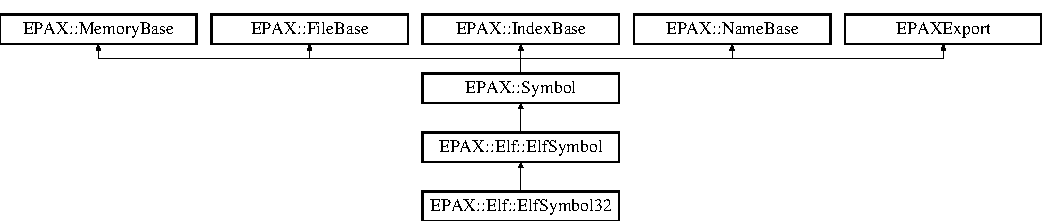
\includegraphics[height=2.966887cm]{class_e_p_a_x_1_1_elf_1_1_elf_symbol32}
\end{center}
\end{figure}
\subsection*{\-Public \-Member \-Functions}
\begin{DoxyCompactItemize}
\item 
\hyperlink{class_e_p_a_x_1_1_elf_1_1_elf_symbol32_a5abc8b081298263bef61b466cbfac2d1}{\-Elf\-Symbol32} (\hyperlink{class_e_p_a_x_1_1_base_binary}{\-Base\-Binary} $\ast$b, uint64\-\_\-t o, uint32\-\_\-t i)
\item 
virtual \hyperlink{class_e_p_a_x_1_1_elf_1_1_elf_symbol32_a355036bd959ec61140192aac8a486750}{$\sim$\-Elf\-Symbol32} ()
\item 
uint64\-\_\-t \hyperlink{class_e_p_a_x_1_1_elf_1_1_elf_symbol32_a319c4e22fbb4b99667707a8b0d9412d1}{get\-Name\-Index} ()
\item 
uint64\-\_\-t \hyperlink{class_e_p_a_x_1_1_elf_1_1_elf_symbol32_a2b4bb23d3d59280ccbbdf0b239bc4ce2}{get\-Value} ()
\item 
uint32\-\_\-t \hyperlink{class_e_p_a_x_1_1_elf_1_1_elf_symbol32_a5ae0934c001dc2a81dbd88fb1d0ad786}{get\-Section} ()
\item 
uint32\-\_\-t \hyperlink{class_e_p_a_x_1_1_elf_1_1_elf_symbol32_ae5ef1d81c0a3d126441e147104f8ea85}{get\-Size} ()
\item 
uint32\-\_\-t \hyperlink{class_e_p_a_x_1_1_elf_1_1_elf_symbol32_a870365328bf8943618c3a3f907f26b24}{get\-Type} ()
\item 
uint32\-\_\-t \hyperlink{class_e_p_a_x_1_1_elf_1_1_elf_symbol32_a9361f33bf04cbfd6623392f1905aaef6}{get\-Binding} ()
\item 
uint64\-\_\-t \hyperlink{class_e_p_a_x_1_1_elf_1_1_elf_symbol32_a547bb437518ff680a5b35c36ebc5e39a}{get\-Visibility} ()
\end{DoxyCompactItemize}


\subsection{\-Detailed \-Description}


\-Definition at line 193 of file \-Elf\-Binary.\-hpp.



\subsection{\-Constructor \& \-Destructor \-Documentation}
\hypertarget{class_e_p_a_x_1_1_elf_1_1_elf_symbol32_a5abc8b081298263bef61b466cbfac2d1}{\index{\-E\-P\-A\-X\-::\-Elf\-::\-Elf\-Symbol32@{\-E\-P\-A\-X\-::\-Elf\-::\-Elf\-Symbol32}!\-Elf\-Symbol32@{\-Elf\-Symbol32}}
\index{\-Elf\-Symbol32@{\-Elf\-Symbol32}!EPAX::Elf::ElfSymbol32@{\-E\-P\-A\-X\-::\-Elf\-::\-Elf\-Symbol32}}
\subsubsection[{\-Elf\-Symbol32}]{\setlength{\rightskip}{0pt plus 5cm}{\bf \-E\-P\-A\-X\-::\-Elf\-::\-Elf\-Symbol32\-::\-Elf\-Symbol32} (
\begin{DoxyParamCaption}
\item[{{\bf \-Base\-Binary} $\ast$}]{b, }
\item[{uint64\-\_\-t}]{o, }
\item[{uint32\-\_\-t}]{i}
\end{DoxyParamCaption}
)}}\label{class_e_p_a_x_1_1_elf_1_1_elf_symbol32_a5abc8b081298263bef61b466cbfac2d1}


\-Definition at line 542 of file \-Elf\-Binary.\-cpp.

\hypertarget{class_e_p_a_x_1_1_elf_1_1_elf_symbol32_a355036bd959ec61140192aac8a486750}{\index{\-E\-P\-A\-X\-::\-Elf\-::\-Elf\-Symbol32@{\-E\-P\-A\-X\-::\-Elf\-::\-Elf\-Symbol32}!$\sim$\-Elf\-Symbol32@{$\sim$\-Elf\-Symbol32}}
\index{$\sim$\-Elf\-Symbol32@{$\sim$\-Elf\-Symbol32}!EPAX::Elf::ElfSymbol32@{\-E\-P\-A\-X\-::\-Elf\-::\-Elf\-Symbol32}}
\subsubsection[{$\sim$\-Elf\-Symbol32}]{\setlength{\rightskip}{0pt plus 5cm}virtual {\bf \-E\-P\-A\-X\-::\-Elf\-::\-Elf\-Symbol32\-::$\sim$\-Elf\-Symbol32} (
\begin{DoxyParamCaption}
{}
\end{DoxyParamCaption}
)\hspace{0.3cm}{\ttfamily  \mbox{[}inline, virtual\mbox{]}}}}\label{class_e_p_a_x_1_1_elf_1_1_elf_symbol32_a355036bd959ec61140192aac8a486750}


\-Definition at line 196 of file \-Elf\-Binary.\-hpp.



\subsection{\-Member \-Function \-Documentation}
\hypertarget{class_e_p_a_x_1_1_elf_1_1_elf_symbol32_a9361f33bf04cbfd6623392f1905aaef6}{\index{\-E\-P\-A\-X\-::\-Elf\-::\-Elf\-Symbol32@{\-E\-P\-A\-X\-::\-Elf\-::\-Elf\-Symbol32}!get\-Binding@{get\-Binding}}
\index{get\-Binding@{get\-Binding}!EPAX::Elf::ElfSymbol32@{\-E\-P\-A\-X\-::\-Elf\-::\-Elf\-Symbol32}}
\subsubsection[{get\-Binding}]{\setlength{\rightskip}{0pt plus 5cm}uint32\-\_\-t {\bf \-E\-P\-A\-X\-::\-Elf\-::\-Elf\-Symbol32\-::get\-Binding} (
\begin{DoxyParamCaption}
{}
\end{DoxyParamCaption}
)\hspace{0.3cm}{\ttfamily  \mbox{[}virtual\mbox{]}}}}\label{class_e_p_a_x_1_1_elf_1_1_elf_symbol32_a9361f33bf04cbfd6623392f1905aaef6}


\-Implements \hyperlink{class_e_p_a_x_1_1_elf_1_1_elf_symbol_a3bed4c1dcd7d20cdd492c16977e59b93}{\-E\-P\-A\-X\-::\-Elf\-::\-Elf\-Symbol}.



\-Definition at line 596 of file \-Elf\-Binary.\-cpp.

\hypertarget{class_e_p_a_x_1_1_elf_1_1_elf_symbol32_a319c4e22fbb4b99667707a8b0d9412d1}{\index{\-E\-P\-A\-X\-::\-Elf\-::\-Elf\-Symbol32@{\-E\-P\-A\-X\-::\-Elf\-::\-Elf\-Symbol32}!get\-Name\-Index@{get\-Name\-Index}}
\index{get\-Name\-Index@{get\-Name\-Index}!EPAX::Elf::ElfSymbol32@{\-E\-P\-A\-X\-::\-Elf\-::\-Elf\-Symbol32}}
\subsubsection[{get\-Name\-Index}]{\setlength{\rightskip}{0pt plus 5cm}uint64\-\_\-t {\bf \-E\-P\-A\-X\-::\-Elf\-::\-Elf\-Symbol32\-::get\-Name\-Index} (
\begin{DoxyParamCaption}
{}
\end{DoxyParamCaption}
)\hspace{0.3cm}{\ttfamily  \mbox{[}virtual\mbox{]}}}}\label{class_e_p_a_x_1_1_elf_1_1_elf_symbol32_a319c4e22fbb4b99667707a8b0d9412d1}


\-Implements \hyperlink{class_e_p_a_x_1_1_elf_1_1_elf_symbol_a84ccb1d566bee093da094e2c4b617ba7}{\-E\-P\-A\-X\-::\-Elf\-::\-Elf\-Symbol}.



\-Definition at line 556 of file \-Elf\-Binary.\-cpp.

\hypertarget{class_e_p_a_x_1_1_elf_1_1_elf_symbol32_a5ae0934c001dc2a81dbd88fb1d0ad786}{\index{\-E\-P\-A\-X\-::\-Elf\-::\-Elf\-Symbol32@{\-E\-P\-A\-X\-::\-Elf\-::\-Elf\-Symbol32}!get\-Section@{get\-Section}}
\index{get\-Section@{get\-Section}!EPAX::Elf::ElfSymbol32@{\-E\-P\-A\-X\-::\-Elf\-::\-Elf\-Symbol32}}
\subsubsection[{get\-Section}]{\setlength{\rightskip}{0pt plus 5cm}uint32\-\_\-t {\bf \-E\-P\-A\-X\-::\-Elf\-::\-Elf\-Symbol32\-::get\-Section} (
\begin{DoxyParamCaption}
{}
\end{DoxyParamCaption}
)\hspace{0.3cm}{\ttfamily  \mbox{[}virtual\mbox{]}}}}\label{class_e_p_a_x_1_1_elf_1_1_elf_symbol32_a5ae0934c001dc2a81dbd88fb1d0ad786}


\-Implements \hyperlink{class_e_p_a_x_1_1_elf_1_1_elf_symbol_a92184692a8f808802963e1a7ca9606d7}{\-E\-P\-A\-X\-::\-Elf\-::\-Elf\-Symbol}.



\-Definition at line 580 of file \-Elf\-Binary.\-cpp.

\hypertarget{class_e_p_a_x_1_1_elf_1_1_elf_symbol32_ae5ef1d81c0a3d126441e147104f8ea85}{\index{\-E\-P\-A\-X\-::\-Elf\-::\-Elf\-Symbol32@{\-E\-P\-A\-X\-::\-Elf\-::\-Elf\-Symbol32}!get\-Size@{get\-Size}}
\index{get\-Size@{get\-Size}!EPAX::Elf::ElfSymbol32@{\-E\-P\-A\-X\-::\-Elf\-::\-Elf\-Symbol32}}
\subsubsection[{get\-Size}]{\setlength{\rightskip}{0pt plus 5cm}uint32\-\_\-t {\bf \-E\-P\-A\-X\-::\-Elf\-::\-Elf\-Symbol32\-::get\-Size} (
\begin{DoxyParamCaption}
{}
\end{DoxyParamCaption}
)\hspace{0.3cm}{\ttfamily  \mbox{[}virtual\mbox{]}}}}\label{class_e_p_a_x_1_1_elf_1_1_elf_symbol32_ae5ef1d81c0a3d126441e147104f8ea85}


\-Implements \hyperlink{class_e_p_a_x_1_1_elf_1_1_elf_symbol_a38fb6985ad991affbb10051eac2aa75e}{\-E\-P\-A\-X\-::\-Elf\-::\-Elf\-Symbol}.



\-Definition at line 572 of file \-Elf\-Binary.\-cpp.

\hypertarget{class_e_p_a_x_1_1_elf_1_1_elf_symbol32_a870365328bf8943618c3a3f907f26b24}{\index{\-E\-P\-A\-X\-::\-Elf\-::\-Elf\-Symbol32@{\-E\-P\-A\-X\-::\-Elf\-::\-Elf\-Symbol32}!get\-Type@{get\-Type}}
\index{get\-Type@{get\-Type}!EPAX::Elf::ElfSymbol32@{\-E\-P\-A\-X\-::\-Elf\-::\-Elf\-Symbol32}}
\subsubsection[{get\-Type}]{\setlength{\rightskip}{0pt plus 5cm}uint32\-\_\-t {\bf \-E\-P\-A\-X\-::\-Elf\-::\-Elf\-Symbol32\-::get\-Type} (
\begin{DoxyParamCaption}
{}
\end{DoxyParamCaption}
)\hspace{0.3cm}{\ttfamily  \mbox{[}virtual\mbox{]}}}}\label{class_e_p_a_x_1_1_elf_1_1_elf_symbol32_a870365328bf8943618c3a3f907f26b24}


\-Implements \hyperlink{class_e_p_a_x_1_1_elf_1_1_elf_symbol_a540aabaf19398d8512f7bdb9255fa9d6}{\-E\-P\-A\-X\-::\-Elf\-::\-Elf\-Symbol}.



\-Definition at line 588 of file \-Elf\-Binary.\-cpp.

\hypertarget{class_e_p_a_x_1_1_elf_1_1_elf_symbol32_a2b4bb23d3d59280ccbbdf0b239bc4ce2}{\index{\-E\-P\-A\-X\-::\-Elf\-::\-Elf\-Symbol32@{\-E\-P\-A\-X\-::\-Elf\-::\-Elf\-Symbol32}!get\-Value@{get\-Value}}
\index{get\-Value@{get\-Value}!EPAX::Elf::ElfSymbol32@{\-E\-P\-A\-X\-::\-Elf\-::\-Elf\-Symbol32}}
\subsubsection[{get\-Value}]{\setlength{\rightskip}{0pt plus 5cm}uint64\-\_\-t {\bf \-E\-P\-A\-X\-::\-Elf\-::\-Elf\-Symbol32\-::get\-Value} (
\begin{DoxyParamCaption}
{}
\end{DoxyParamCaption}
)\hspace{0.3cm}{\ttfamily  \mbox{[}virtual\mbox{]}}}}\label{class_e_p_a_x_1_1_elf_1_1_elf_symbol32_a2b4bb23d3d59280ccbbdf0b239bc4ce2}


\-Implements \hyperlink{class_e_p_a_x_1_1_elf_1_1_elf_symbol_a20b9df356b7d4ef1481dc8fdeaf4b2fc}{\-E\-P\-A\-X\-::\-Elf\-::\-Elf\-Symbol}.



\-Definition at line 564 of file \-Elf\-Binary.\-cpp.

\hypertarget{class_e_p_a_x_1_1_elf_1_1_elf_symbol32_a547bb437518ff680a5b35c36ebc5e39a}{\index{\-E\-P\-A\-X\-::\-Elf\-::\-Elf\-Symbol32@{\-E\-P\-A\-X\-::\-Elf\-::\-Elf\-Symbol32}!get\-Visibility@{get\-Visibility}}
\index{get\-Visibility@{get\-Visibility}!EPAX::Elf::ElfSymbol32@{\-E\-P\-A\-X\-::\-Elf\-::\-Elf\-Symbol32}}
\subsubsection[{get\-Visibility}]{\setlength{\rightskip}{0pt plus 5cm}uint64\-\_\-t {\bf \-E\-P\-A\-X\-::\-Elf\-::\-Elf\-Symbol32\-::get\-Visibility} (
\begin{DoxyParamCaption}
{}
\end{DoxyParamCaption}
)\hspace{0.3cm}{\ttfamily  \mbox{[}virtual\mbox{]}}}}\label{class_e_p_a_x_1_1_elf_1_1_elf_symbol32_a547bb437518ff680a5b35c36ebc5e39a}


\-Implements \hyperlink{class_e_p_a_x_1_1_elf_1_1_elf_symbol_a31b56e39f50f311ab23e878faba5d5b4}{\-E\-P\-A\-X\-::\-Elf\-::\-Elf\-Symbol}.



\-Definition at line 604 of file \-Elf\-Binary.\-cpp.



\-The documentation for this class was generated from the following files\-:\begin{DoxyCompactItemize}
\item 
\hyperlink{_elf_binary_8hpp}{\-Elf\-Binary.\-hpp}\item 
\hyperlink{_elf_binary_8cpp}{\-Elf\-Binary.\-cpp}\end{DoxyCompactItemize}

\hypertarget{class_e_p_a_x_1_1_elf_1_1_elf_symbol64}{\section{\-E\-P\-A\-X\-:\-:\-Elf\-:\-:\-Elf\-Symbol64 \-Class \-Reference}
\label{class_e_p_a_x_1_1_elf_1_1_elf_symbol64}\index{\-E\-P\-A\-X\-::\-Elf\-::\-Elf\-Symbol64@{\-E\-P\-A\-X\-::\-Elf\-::\-Elf\-Symbol64}}
}


{\ttfamily \#include $<$\-Elf\-Binary.\-hpp$>$}

\-Inheritance diagram for \-E\-P\-A\-X\-:\-:\-Elf\-:\-:\-Elf\-Symbol64\-:\begin{figure}[H]
\begin{center}
\leavevmode
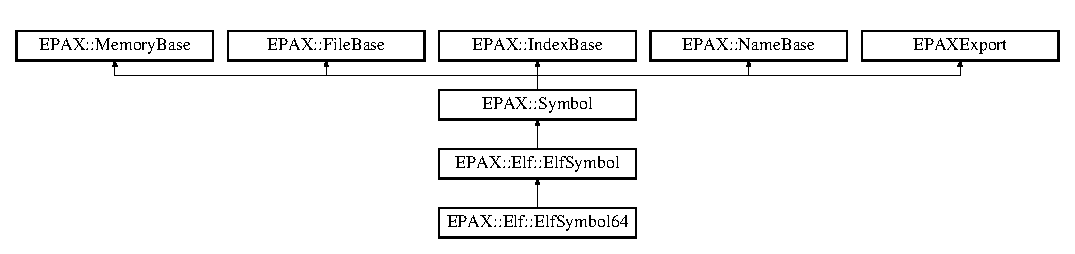
\includegraphics[height=2.966887cm]{class_e_p_a_x_1_1_elf_1_1_elf_symbol64}
\end{center}
\end{figure}
\subsection*{\-Public \-Member \-Functions}
\begin{DoxyCompactItemize}
\item 
\hyperlink{class_e_p_a_x_1_1_elf_1_1_elf_symbol64_a6a2d4c76afce4bb068cff341c55f88a3}{\-Elf\-Symbol64} (\hyperlink{class_e_p_a_x_1_1_base_binary}{\-Base\-Binary} $\ast$b, uint64\-\_\-t o, uint32\-\_\-t i)
\item 
virtual \hyperlink{class_e_p_a_x_1_1_elf_1_1_elf_symbol64_a1f755b0726bba59f8965d37449658121}{$\sim$\-Elf\-Symbol64} ()
\item 
uint64\-\_\-t \hyperlink{class_e_p_a_x_1_1_elf_1_1_elf_symbol64_a6e8651a83dfdd485e87e013b4a4790e2}{get\-Name\-Index} ()
\item 
uint64\-\_\-t \hyperlink{class_e_p_a_x_1_1_elf_1_1_elf_symbol64_a47e49dde9967bc7cf3f8caeb3b1880fd}{get\-Value} ()
\item 
uint32\-\_\-t \hyperlink{class_e_p_a_x_1_1_elf_1_1_elf_symbol64_ad2acb7dbbf88685b5bfcfbed2ac1dba4}{get\-Section} ()
\item 
uint32\-\_\-t \hyperlink{class_e_p_a_x_1_1_elf_1_1_elf_symbol64_a26225a3989efc89a50fa934c53f47276}{get\-Size} ()
\item 
uint32\-\_\-t \hyperlink{class_e_p_a_x_1_1_elf_1_1_elf_symbol64_a397faa7562b27ba2d543328a69e17077}{get\-Type} ()
\item 
uint32\-\_\-t \hyperlink{class_e_p_a_x_1_1_elf_1_1_elf_symbol64_a341e642319d9b9f70ee9dfebdcad4f5b}{get\-Binding} ()
\item 
uint64\-\_\-t \hyperlink{class_e_p_a_x_1_1_elf_1_1_elf_symbol64_a0df4c678ba3e7c3e756c6a81152244fa}{get\-Visibility} ()
\end{DoxyCompactItemize}


\subsection{\-Detailed \-Description}


\-Definition at line 208 of file \-Elf\-Binary.\-hpp.



\subsection{\-Constructor \& \-Destructor \-Documentation}
\hypertarget{class_e_p_a_x_1_1_elf_1_1_elf_symbol64_a6a2d4c76afce4bb068cff341c55f88a3}{\index{\-E\-P\-A\-X\-::\-Elf\-::\-Elf\-Symbol64@{\-E\-P\-A\-X\-::\-Elf\-::\-Elf\-Symbol64}!\-Elf\-Symbol64@{\-Elf\-Symbol64}}
\index{\-Elf\-Symbol64@{\-Elf\-Symbol64}!EPAX::Elf::ElfSymbol64@{\-E\-P\-A\-X\-::\-Elf\-::\-Elf\-Symbol64}}
\subsubsection[{\-Elf\-Symbol64}]{\setlength{\rightskip}{0pt plus 5cm}{\bf \-E\-P\-A\-X\-::\-Elf\-::\-Elf\-Symbol64\-::\-Elf\-Symbol64} (
\begin{DoxyParamCaption}
\item[{{\bf \-Base\-Binary} $\ast$}]{b, }
\item[{uint64\-\_\-t}]{o, }
\item[{uint32\-\_\-t}]{i}
\end{DoxyParamCaption}
)}}\label{class_e_p_a_x_1_1_elf_1_1_elf_symbol64_a6a2d4c76afce4bb068cff341c55f88a3}


\-Definition at line 549 of file \-Elf\-Binary.\-cpp.

\hypertarget{class_e_p_a_x_1_1_elf_1_1_elf_symbol64_a1f755b0726bba59f8965d37449658121}{\index{\-E\-P\-A\-X\-::\-Elf\-::\-Elf\-Symbol64@{\-E\-P\-A\-X\-::\-Elf\-::\-Elf\-Symbol64}!$\sim$\-Elf\-Symbol64@{$\sim$\-Elf\-Symbol64}}
\index{$\sim$\-Elf\-Symbol64@{$\sim$\-Elf\-Symbol64}!EPAX::Elf::ElfSymbol64@{\-E\-P\-A\-X\-::\-Elf\-::\-Elf\-Symbol64}}
\subsubsection[{$\sim$\-Elf\-Symbol64}]{\setlength{\rightskip}{0pt plus 5cm}virtual {\bf \-E\-P\-A\-X\-::\-Elf\-::\-Elf\-Symbol64\-::$\sim$\-Elf\-Symbol64} (
\begin{DoxyParamCaption}
{}
\end{DoxyParamCaption}
)\hspace{0.3cm}{\ttfamily  \mbox{[}inline, virtual\mbox{]}}}}\label{class_e_p_a_x_1_1_elf_1_1_elf_symbol64_a1f755b0726bba59f8965d37449658121}


\-Definition at line 211 of file \-Elf\-Binary.\-hpp.



\subsection{\-Member \-Function \-Documentation}
\hypertarget{class_e_p_a_x_1_1_elf_1_1_elf_symbol64_a341e642319d9b9f70ee9dfebdcad4f5b}{\index{\-E\-P\-A\-X\-::\-Elf\-::\-Elf\-Symbol64@{\-E\-P\-A\-X\-::\-Elf\-::\-Elf\-Symbol64}!get\-Binding@{get\-Binding}}
\index{get\-Binding@{get\-Binding}!EPAX::Elf::ElfSymbol64@{\-E\-P\-A\-X\-::\-Elf\-::\-Elf\-Symbol64}}
\subsubsection[{get\-Binding}]{\setlength{\rightskip}{0pt plus 5cm}uint32\-\_\-t {\bf \-E\-P\-A\-X\-::\-Elf\-::\-Elf\-Symbol64\-::get\-Binding} (
\begin{DoxyParamCaption}
{}
\end{DoxyParamCaption}
)\hspace{0.3cm}{\ttfamily  \mbox{[}virtual\mbox{]}}}}\label{class_e_p_a_x_1_1_elf_1_1_elf_symbol64_a341e642319d9b9f70ee9dfebdcad4f5b}


\-Implements \hyperlink{class_e_p_a_x_1_1_elf_1_1_elf_symbol_a3bed4c1dcd7d20cdd492c16977e59b93}{\-E\-P\-A\-X\-::\-Elf\-::\-Elf\-Symbol}.



\-Definition at line 600 of file \-Elf\-Binary.\-cpp.

\hypertarget{class_e_p_a_x_1_1_elf_1_1_elf_symbol64_a6e8651a83dfdd485e87e013b4a4790e2}{\index{\-E\-P\-A\-X\-::\-Elf\-::\-Elf\-Symbol64@{\-E\-P\-A\-X\-::\-Elf\-::\-Elf\-Symbol64}!get\-Name\-Index@{get\-Name\-Index}}
\index{get\-Name\-Index@{get\-Name\-Index}!EPAX::Elf::ElfSymbol64@{\-E\-P\-A\-X\-::\-Elf\-::\-Elf\-Symbol64}}
\subsubsection[{get\-Name\-Index}]{\setlength{\rightskip}{0pt plus 5cm}uint64\-\_\-t {\bf \-E\-P\-A\-X\-::\-Elf\-::\-Elf\-Symbol64\-::get\-Name\-Index} (
\begin{DoxyParamCaption}
{}
\end{DoxyParamCaption}
)\hspace{0.3cm}{\ttfamily  \mbox{[}virtual\mbox{]}}}}\label{class_e_p_a_x_1_1_elf_1_1_elf_symbol64_a6e8651a83dfdd485e87e013b4a4790e2}


\-Implements \hyperlink{class_e_p_a_x_1_1_elf_1_1_elf_symbol_a84ccb1d566bee093da094e2c4b617ba7}{\-E\-P\-A\-X\-::\-Elf\-::\-Elf\-Symbol}.



\-Definition at line 560 of file \-Elf\-Binary.\-cpp.

\hypertarget{class_e_p_a_x_1_1_elf_1_1_elf_symbol64_ad2acb7dbbf88685b5bfcfbed2ac1dba4}{\index{\-E\-P\-A\-X\-::\-Elf\-::\-Elf\-Symbol64@{\-E\-P\-A\-X\-::\-Elf\-::\-Elf\-Symbol64}!get\-Section@{get\-Section}}
\index{get\-Section@{get\-Section}!EPAX::Elf::ElfSymbol64@{\-E\-P\-A\-X\-::\-Elf\-::\-Elf\-Symbol64}}
\subsubsection[{get\-Section}]{\setlength{\rightskip}{0pt plus 5cm}uint32\-\_\-t {\bf \-E\-P\-A\-X\-::\-Elf\-::\-Elf\-Symbol64\-::get\-Section} (
\begin{DoxyParamCaption}
{}
\end{DoxyParamCaption}
)\hspace{0.3cm}{\ttfamily  \mbox{[}virtual\mbox{]}}}}\label{class_e_p_a_x_1_1_elf_1_1_elf_symbol64_ad2acb7dbbf88685b5bfcfbed2ac1dba4}


\-Implements \hyperlink{class_e_p_a_x_1_1_elf_1_1_elf_symbol_a92184692a8f808802963e1a7ca9606d7}{\-E\-P\-A\-X\-::\-Elf\-::\-Elf\-Symbol}.



\-Definition at line 584 of file \-Elf\-Binary.\-cpp.

\hypertarget{class_e_p_a_x_1_1_elf_1_1_elf_symbol64_a26225a3989efc89a50fa934c53f47276}{\index{\-E\-P\-A\-X\-::\-Elf\-::\-Elf\-Symbol64@{\-E\-P\-A\-X\-::\-Elf\-::\-Elf\-Symbol64}!get\-Size@{get\-Size}}
\index{get\-Size@{get\-Size}!EPAX::Elf::ElfSymbol64@{\-E\-P\-A\-X\-::\-Elf\-::\-Elf\-Symbol64}}
\subsubsection[{get\-Size}]{\setlength{\rightskip}{0pt plus 5cm}uint32\-\_\-t {\bf \-E\-P\-A\-X\-::\-Elf\-::\-Elf\-Symbol64\-::get\-Size} (
\begin{DoxyParamCaption}
{}
\end{DoxyParamCaption}
)\hspace{0.3cm}{\ttfamily  \mbox{[}virtual\mbox{]}}}}\label{class_e_p_a_x_1_1_elf_1_1_elf_symbol64_a26225a3989efc89a50fa934c53f47276}


\-Implements \hyperlink{class_e_p_a_x_1_1_elf_1_1_elf_symbol_a38fb6985ad991affbb10051eac2aa75e}{\-E\-P\-A\-X\-::\-Elf\-::\-Elf\-Symbol}.



\-Definition at line 576 of file \-Elf\-Binary.\-cpp.

\hypertarget{class_e_p_a_x_1_1_elf_1_1_elf_symbol64_a397faa7562b27ba2d543328a69e17077}{\index{\-E\-P\-A\-X\-::\-Elf\-::\-Elf\-Symbol64@{\-E\-P\-A\-X\-::\-Elf\-::\-Elf\-Symbol64}!get\-Type@{get\-Type}}
\index{get\-Type@{get\-Type}!EPAX::Elf::ElfSymbol64@{\-E\-P\-A\-X\-::\-Elf\-::\-Elf\-Symbol64}}
\subsubsection[{get\-Type}]{\setlength{\rightskip}{0pt plus 5cm}uint32\-\_\-t {\bf \-E\-P\-A\-X\-::\-Elf\-::\-Elf\-Symbol64\-::get\-Type} (
\begin{DoxyParamCaption}
{}
\end{DoxyParamCaption}
)\hspace{0.3cm}{\ttfamily  \mbox{[}virtual\mbox{]}}}}\label{class_e_p_a_x_1_1_elf_1_1_elf_symbol64_a397faa7562b27ba2d543328a69e17077}


\-Implements \hyperlink{class_e_p_a_x_1_1_elf_1_1_elf_symbol_a540aabaf19398d8512f7bdb9255fa9d6}{\-E\-P\-A\-X\-::\-Elf\-::\-Elf\-Symbol}.



\-Definition at line 592 of file \-Elf\-Binary.\-cpp.

\hypertarget{class_e_p_a_x_1_1_elf_1_1_elf_symbol64_a47e49dde9967bc7cf3f8caeb3b1880fd}{\index{\-E\-P\-A\-X\-::\-Elf\-::\-Elf\-Symbol64@{\-E\-P\-A\-X\-::\-Elf\-::\-Elf\-Symbol64}!get\-Value@{get\-Value}}
\index{get\-Value@{get\-Value}!EPAX::Elf::ElfSymbol64@{\-E\-P\-A\-X\-::\-Elf\-::\-Elf\-Symbol64}}
\subsubsection[{get\-Value}]{\setlength{\rightskip}{0pt plus 5cm}uint64\-\_\-t {\bf \-E\-P\-A\-X\-::\-Elf\-::\-Elf\-Symbol64\-::get\-Value} (
\begin{DoxyParamCaption}
{}
\end{DoxyParamCaption}
)\hspace{0.3cm}{\ttfamily  \mbox{[}virtual\mbox{]}}}}\label{class_e_p_a_x_1_1_elf_1_1_elf_symbol64_a47e49dde9967bc7cf3f8caeb3b1880fd}


\-Implements \hyperlink{class_e_p_a_x_1_1_elf_1_1_elf_symbol_a20b9df356b7d4ef1481dc8fdeaf4b2fc}{\-E\-P\-A\-X\-::\-Elf\-::\-Elf\-Symbol}.



\-Definition at line 568 of file \-Elf\-Binary.\-cpp.

\hypertarget{class_e_p_a_x_1_1_elf_1_1_elf_symbol64_a0df4c678ba3e7c3e756c6a81152244fa}{\index{\-E\-P\-A\-X\-::\-Elf\-::\-Elf\-Symbol64@{\-E\-P\-A\-X\-::\-Elf\-::\-Elf\-Symbol64}!get\-Visibility@{get\-Visibility}}
\index{get\-Visibility@{get\-Visibility}!EPAX::Elf::ElfSymbol64@{\-E\-P\-A\-X\-::\-Elf\-::\-Elf\-Symbol64}}
\subsubsection[{get\-Visibility}]{\setlength{\rightskip}{0pt plus 5cm}uint64\-\_\-t {\bf \-E\-P\-A\-X\-::\-Elf\-::\-Elf\-Symbol64\-::get\-Visibility} (
\begin{DoxyParamCaption}
{}
\end{DoxyParamCaption}
)\hspace{0.3cm}{\ttfamily  \mbox{[}virtual\mbox{]}}}}\label{class_e_p_a_x_1_1_elf_1_1_elf_symbol64_a0df4c678ba3e7c3e756c6a81152244fa}


\-Implements \hyperlink{class_e_p_a_x_1_1_elf_1_1_elf_symbol_a31b56e39f50f311ab23e878faba5d5b4}{\-E\-P\-A\-X\-::\-Elf\-::\-Elf\-Symbol}.



\-Definition at line 608 of file \-Elf\-Binary.\-cpp.



\-The documentation for this class was generated from the following files\-:\begin{DoxyCompactItemize}
\item 
\hyperlink{_elf_binary_8hpp}{\-Elf\-Binary.\-hpp}\item 
\hyperlink{_elf_binary_8cpp}{\-Elf\-Binary.\-cpp}\end{DoxyCompactItemize}

\hypertarget{class_e_p_a_x_1_1_elf_1_1_elf_symbol_table}{\section{\-E\-P\-A\-X\-:\-:\-Elf\-:\-:\-Elf\-Symbol\-Table \-Class \-Reference}
\label{class_e_p_a_x_1_1_elf_1_1_elf_symbol_table}\index{\-E\-P\-A\-X\-::\-Elf\-::\-Elf\-Symbol\-Table@{\-E\-P\-A\-X\-::\-Elf\-::\-Elf\-Symbol\-Table}}
}


{\ttfamily \#include $<$\-Elf\-Binary.\-hpp$>$}

\-Inheritance diagram for \-E\-P\-A\-X\-:\-:\-Elf\-:\-:\-Elf\-Symbol\-Table\-:\begin{figure}[H]
\begin{center}
\leavevmode
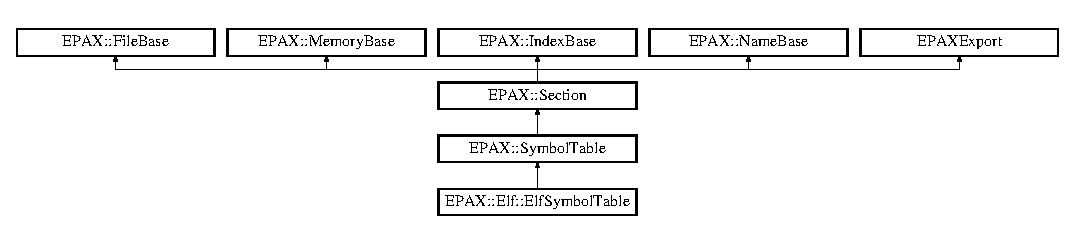
\includegraphics[height=2.666667cm]{class_e_p_a_x_1_1_elf_1_1_elf_symbol_table}
\end{center}
\end{figure}
\subsection*{\-Public \-Member \-Functions}
\begin{DoxyCompactItemize}
\item 
\hyperlink{class_e_p_a_x_1_1_elf_1_1_elf_symbol_table_a33103257dce585b4f3ace8cad4bb0d8d}{\-Elf\-Symbol\-Table} (\hyperlink{class_e_p_a_x_1_1_base_binary}{\-Base\-Binary} $\ast$b, uint64\-\_\-t o, uint64\-\_\-t fs, uint64\-\_\-t ma, uint64\-\_\-t ms, uint32\-\_\-t i, std\-::string n, \hyperlink{class_e_p_a_x_1_1_elf_1_1_elf_string_table}{\-Elf\-String\-Table} $\ast$st)
\item 
\hyperlink{class_e_p_a_x_1_1_elf_1_1_elf_symbol_table_a4442dcddc38d01ec99a4d7dd29fe9a9f}{$\sim$\-Elf\-Symbol\-Table} ()
\item 
void \hyperlink{class_e_p_a_x_1_1_elf_1_1_elf_symbol_table_af8c0bb17c3b8c38ee49142def9ee0ed0}{print} (std\-::ostream \&stream=std\-::cout)
\end{DoxyCompactItemize}


\subsection{\-Detailed \-Description}


\-Definition at line 236 of file \-Elf\-Binary.\-hpp.



\subsection{\-Constructor \& \-Destructor \-Documentation}
\hypertarget{class_e_p_a_x_1_1_elf_1_1_elf_symbol_table_a33103257dce585b4f3ace8cad4bb0d8d}{\index{\-E\-P\-A\-X\-::\-Elf\-::\-Elf\-Symbol\-Table@{\-E\-P\-A\-X\-::\-Elf\-::\-Elf\-Symbol\-Table}!\-Elf\-Symbol\-Table@{\-Elf\-Symbol\-Table}}
\index{\-Elf\-Symbol\-Table@{\-Elf\-Symbol\-Table}!EPAX::Elf::ElfSymbolTable@{\-E\-P\-A\-X\-::\-Elf\-::\-Elf\-Symbol\-Table}}
\subsubsection[{\-Elf\-Symbol\-Table}]{\setlength{\rightskip}{0pt plus 5cm}{\bf \-E\-P\-A\-X\-::\-Elf\-::\-Elf\-Symbol\-Table\-::\-Elf\-Symbol\-Table} (
\begin{DoxyParamCaption}
\item[{{\bf \-Base\-Binary} $\ast$}]{b, }
\item[{uint64\-\_\-t}]{o, }
\item[{uint64\-\_\-t}]{fs, }
\item[{uint64\-\_\-t}]{ma, }
\item[{uint64\-\_\-t}]{ms, }
\item[{uint32\-\_\-t}]{i, }
\item[{std\-::string}]{n, }
\item[{{\bf \-Elf\-String\-Table} $\ast$}]{st}
\end{DoxyParamCaption}
)}}\label{class_e_p_a_x_1_1_elf_1_1_elf_symbol_table_a33103257dce585b4f3ace8cad4bb0d8d}


\-Definition at line 649 of file \-Elf\-Binary.\-cpp.

\hypertarget{class_e_p_a_x_1_1_elf_1_1_elf_symbol_table_a4442dcddc38d01ec99a4d7dd29fe9a9f}{\index{\-E\-P\-A\-X\-::\-Elf\-::\-Elf\-Symbol\-Table@{\-E\-P\-A\-X\-::\-Elf\-::\-Elf\-Symbol\-Table}!$\sim$\-Elf\-Symbol\-Table@{$\sim$\-Elf\-Symbol\-Table}}
\index{$\sim$\-Elf\-Symbol\-Table@{$\sim$\-Elf\-Symbol\-Table}!EPAX::Elf::ElfSymbolTable@{\-E\-P\-A\-X\-::\-Elf\-::\-Elf\-Symbol\-Table}}
\subsubsection[{$\sim$\-Elf\-Symbol\-Table}]{\setlength{\rightskip}{0pt plus 5cm}{\bf \-E\-P\-A\-X\-::\-Elf\-::\-Elf\-Symbol\-Table\-::$\sim$\-Elf\-Symbol\-Table} (
\begin{DoxyParamCaption}
{}
\end{DoxyParamCaption}
)\hspace{0.3cm}{\ttfamily  \mbox{[}inline\mbox{]}}}}\label{class_e_p_a_x_1_1_elf_1_1_elf_symbol_table_a4442dcddc38d01ec99a4d7dd29fe9a9f}


\-Definition at line 242 of file \-Elf\-Binary.\-hpp.



\subsection{\-Member \-Function \-Documentation}
\hypertarget{class_e_p_a_x_1_1_elf_1_1_elf_symbol_table_af8c0bb17c3b8c38ee49142def9ee0ed0}{\index{\-E\-P\-A\-X\-::\-Elf\-::\-Elf\-Symbol\-Table@{\-E\-P\-A\-X\-::\-Elf\-::\-Elf\-Symbol\-Table}!print@{print}}
\index{print@{print}!EPAX::Elf::ElfSymbolTable@{\-E\-P\-A\-X\-::\-Elf\-::\-Elf\-Symbol\-Table}}
\subsubsection[{print}]{\setlength{\rightskip}{0pt plus 5cm}void {\bf \-E\-P\-A\-X\-::\-Elf\-::\-Elf\-Symbol\-Table\-::print} (
\begin{DoxyParamCaption}
\item[{std\-::ostream \&}]{stream = {\ttfamily std\-:\-:cout}}
\end{DoxyParamCaption}
)\hspace{0.3cm}{\ttfamily  \mbox{[}virtual\mbox{]}}}}\label{class_e_p_a_x_1_1_elf_1_1_elf_symbol_table_af8c0bb17c3b8c38ee49142def9ee0ed0}


\-Implements \hyperlink{class_e_p_a_x_1_1_symbol_table_ac8a581679e678f1472bf684fdf877b9a}{\-E\-P\-A\-X\-::\-Symbol\-Table}.



\-Definition at line 518 of file \-Elf\-Binary.\-cpp.



\-The documentation for this class was generated from the following files\-:\begin{DoxyCompactItemize}
\item 
\hyperlink{_elf_binary_8hpp}{\-Elf\-Binary.\-hpp}\item 
\hyperlink{_elf_binary_8cpp}{\-Elf\-Binary.\-cpp}\end{DoxyCompactItemize}

\hypertarget{class_e_p_a_x_export}{\section{\-E\-P\-A\-X\-Export \-Class \-Reference}
\label{class_e_p_a_x_export}\index{\-E\-P\-A\-X\-Export@{\-E\-P\-A\-X\-Export}}
}


{\ttfamily \#include $<$\-E\-P\-A\-X\-Common\-Internal.\-hpp$>$}

\-Inheritance diagram for \-E\-P\-A\-X\-Export\-:\begin{figure}[H]
\begin{center}
\leavevmode
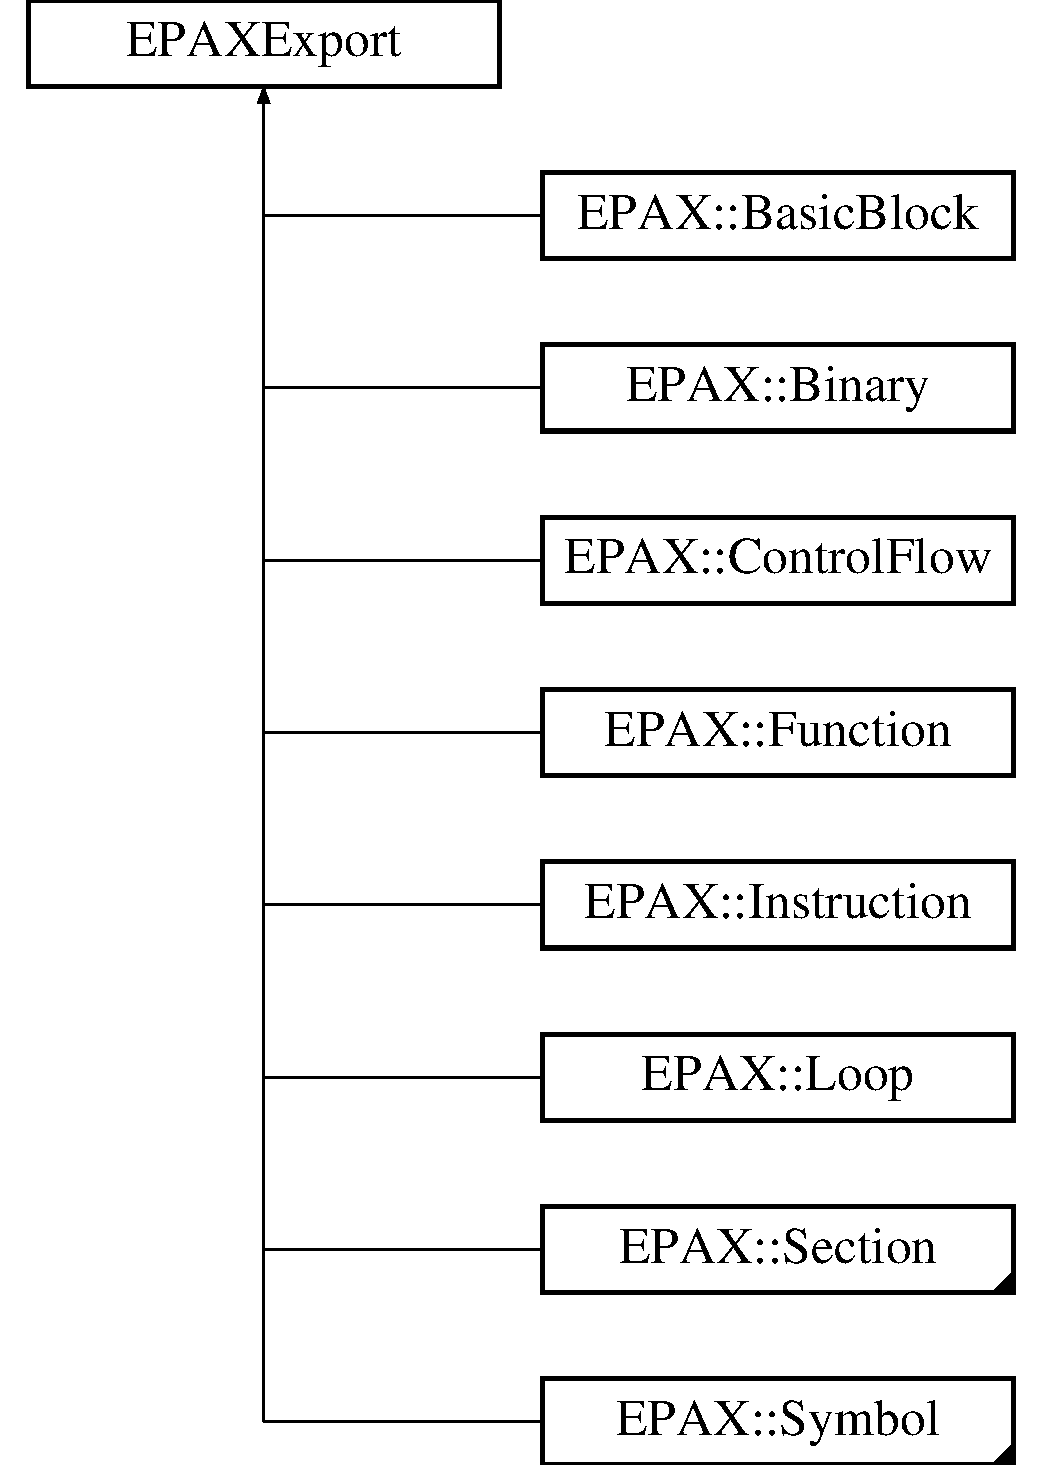
\includegraphics[height=9.000000cm]{class_e_p_a_x_export}
\end{center}
\end{figure}
\subsection*{\-Public \-Member \-Functions}
\begin{DoxyCompactItemize}
\item 
\hyperlink{class_e_p_a_x_export_a72a477fc66fff1f008d38f96a4dc9566}{\-E\-P\-A\-X\-Export} (\hyperlink{_e_p_a_x_common_internal_8hpp_a9cc5d1140a7b3f3840983c0e1a032376}{\-E\-P\-A\-X\-Export\-Class} cls)
\item 
virtual \hyperlink{class_e_p_a_x_export_a6c62eeeea2db1ea174d4760a42cf9ce9}{$\sim$\-E\-P\-A\-X\-Export} ()
\item 
\hyperlink{_e_p_a_x_common_internal_8hpp_a9cc5d1140a7b3f3840983c0e1a032376}{\-E\-P\-A\-X\-Export\-Class} \hyperlink{class_e_p_a_x_export_a87de711519f311339e8db0182630de60}{get\-Class} ()
\end{DoxyCompactItemize}
\subsection*{\-Protected \-Attributes}
\begin{DoxyCompactItemize}
\item 
\hyperlink{_e_p_a_x_common_internal_8hpp_a9cc5d1140a7b3f3840983c0e1a032376}{\-E\-P\-A\-X\-Export\-Class} \hyperlink{class_e_p_a_x_export_a0b819fdbc67897b2d5499c05fa850f29}{expclass}
\end{DoxyCompactItemize}


\subsection{\-Detailed \-Description}


\-Definition at line 112 of file \-E\-P\-A\-X\-Common\-Internal.\-hpp.



\subsection{\-Constructor \& \-Destructor \-Documentation}
\hypertarget{class_e_p_a_x_export_a72a477fc66fff1f008d38f96a4dc9566}{\index{\-E\-P\-A\-X\-Export@{\-E\-P\-A\-X\-Export}!\-E\-P\-A\-X\-Export@{\-E\-P\-A\-X\-Export}}
\index{\-E\-P\-A\-X\-Export@{\-E\-P\-A\-X\-Export}!EPAXExport@{\-E\-P\-A\-X\-Export}}
\subsubsection[{\-E\-P\-A\-X\-Export}]{\setlength{\rightskip}{0pt plus 5cm}{\bf \-E\-P\-A\-X\-Export\-::\-E\-P\-A\-X\-Export} (
\begin{DoxyParamCaption}
\item[{{\bf \-E\-P\-A\-X\-Export\-Class}}]{cls}
\end{DoxyParamCaption}
)\hspace{0.3cm}{\ttfamily  \mbox{[}inline\mbox{]}}}}\label{class_e_p_a_x_export_a72a477fc66fff1f008d38f96a4dc9566}


\-Definition at line 116 of file \-E\-P\-A\-X\-Common\-Internal.\-hpp.

\hypertarget{class_e_p_a_x_export_a6c62eeeea2db1ea174d4760a42cf9ce9}{\index{\-E\-P\-A\-X\-Export@{\-E\-P\-A\-X\-Export}!$\sim$\-E\-P\-A\-X\-Export@{$\sim$\-E\-P\-A\-X\-Export}}
\index{$\sim$\-E\-P\-A\-X\-Export@{$\sim$\-E\-P\-A\-X\-Export}!EPAXExport@{\-E\-P\-A\-X\-Export}}
\subsubsection[{$\sim$\-E\-P\-A\-X\-Export}]{\setlength{\rightskip}{0pt plus 5cm}virtual {\bf \-E\-P\-A\-X\-Export\-::$\sim$\-E\-P\-A\-X\-Export} (
\begin{DoxyParamCaption}
{}
\end{DoxyParamCaption}
)\hspace{0.3cm}{\ttfamily  \mbox{[}inline, virtual\mbox{]}}}}\label{class_e_p_a_x_export_a6c62eeeea2db1ea174d4760a42cf9ce9}


\-Definition at line 117 of file \-E\-P\-A\-X\-Common\-Internal.\-hpp.



\subsection{\-Member \-Function \-Documentation}
\hypertarget{class_e_p_a_x_export_a87de711519f311339e8db0182630de60}{\index{\-E\-P\-A\-X\-Export@{\-E\-P\-A\-X\-Export}!get\-Class@{get\-Class}}
\index{get\-Class@{get\-Class}!EPAXExport@{\-E\-P\-A\-X\-Export}}
\subsubsection[{get\-Class}]{\setlength{\rightskip}{0pt plus 5cm}{\bf \-E\-P\-A\-X\-Export\-Class} {\bf \-E\-P\-A\-X\-Export\-::get\-Class} (
\begin{DoxyParamCaption}
{}
\end{DoxyParamCaption}
)\hspace{0.3cm}{\ttfamily  \mbox{[}inline\mbox{]}}}}\label{class_e_p_a_x_export_a87de711519f311339e8db0182630de60}


\-Definition at line 119 of file \-E\-P\-A\-X\-Common\-Internal.\-hpp.



\subsection{\-Member \-Data \-Documentation}
\hypertarget{class_e_p_a_x_export_a0b819fdbc67897b2d5499c05fa850f29}{\index{\-E\-P\-A\-X\-Export@{\-E\-P\-A\-X\-Export}!expclass@{expclass}}
\index{expclass@{expclass}!EPAXExport@{\-E\-P\-A\-X\-Export}}
\subsubsection[{expclass}]{\setlength{\rightskip}{0pt plus 5cm}{\bf \-E\-P\-A\-X\-Export\-Class} {\bf \-E\-P\-A\-X\-Export\-::expclass}\hspace{0.3cm}{\ttfamily  \mbox{[}protected\mbox{]}}}}\label{class_e_p_a_x_export_a0b819fdbc67897b2d5499c05fa850f29}


\-Definition at line 114 of file \-E\-P\-A\-X\-Common\-Internal.\-hpp.



\-The documentation for this class was generated from the following file\-:\begin{DoxyCompactItemize}
\item 
\hyperlink{_e_p_a_x_common_internal_8hpp}{\-E\-P\-A\-X\-Common\-Internal.\-hpp}\end{DoxyCompactItemize}

\hypertarget{class_e_p_a_x_1_1_file_base}{\section{\-E\-P\-A\-X\-:\-:\-File\-Base \-Class \-Reference}
\label{class_e_p_a_x_1_1_file_base}\index{\-E\-P\-A\-X\-::\-File\-Base@{\-E\-P\-A\-X\-::\-File\-Base}}
}


{\ttfamily \#include $<$\-Base\-Class.\-hpp$>$}

\-Inheritance diagram for \-E\-P\-A\-X\-:\-:\-File\-Base\-:\begin{figure}[H]
\begin{center}
\leavevmode
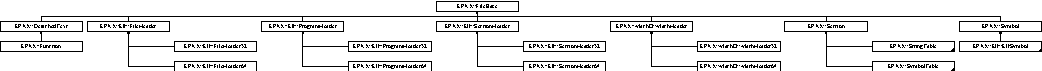
\includegraphics[height=0.952381cm]{class_e_p_a_x_1_1_file_base}
\end{center}
\end{figure}
\subsection*{\-Public \-Member \-Functions}
\begin{DoxyCompactItemize}
\item 
\hyperlink{class_e_p_a_x_1_1_file_base_a9f38ebc8164735bee43367806d76630d}{\-File\-Base} (\hyperlink{class_e_p_a_x_1_1_base_binary}{\-Base\-Binary} $\ast$b, uint64\-\_\-t o, uint64\-\_\-t s)
\item 
virtual \hyperlink{class_e_p_a_x_1_1_file_base_abf99ce91ed574b549d53a1ba43f931ba}{$\sim$\-File\-Base} ()
\item 
\hyperlink{class_e_p_a_x_1_1_base_binary}{\-Base\-Binary} $\ast$ \hyperlink{class_e_p_a_x_1_1_file_base_a2b31d9b96a82c8702aa2e20017039fd4}{get\-Binary} ()
\item 
\hyperlink{class_e_p_a_x_1_1_input_file}{\-Input\-File} $\ast$ \hyperlink{class_e_p_a_x_1_1_file_base_a996b93e64d317be72461c20089a1e91a}{get\-Input\-File} ()
\item 
bool \hyperlink{class_e_p_a_x_1_1_file_base_ab5c2b2dfb21a45a07121d3c0f7942e8b}{is32\-Bit} ()
\item 
uint64\-\_\-t \hyperlink{class_e_p_a_x_1_1_file_base_a779f2254eef1279f52f372e18bfb75f7}{get\-File\-Offset} ()
\item 
uint64\-\_\-t \hyperlink{class_e_p_a_x_1_1_file_base_a41637ea5355a70fee2467f279964e064}{get\-File\-Size} ()
\item 
void \hyperlink{class_e_p_a_x_1_1_file_base_a31b7e5375af339e1bbe998824bfd62f8}{set\-File\-Size} (uint64\-\_\-t s)
\end{DoxyCompactItemize}


\subsection{\-Detailed \-Description}


\-Definition at line 42 of file \-Base\-Class.\-hpp.



\subsection{\-Constructor \& \-Destructor \-Documentation}
\hypertarget{class_e_p_a_x_1_1_file_base_a9f38ebc8164735bee43367806d76630d}{\index{\-E\-P\-A\-X\-::\-File\-Base@{\-E\-P\-A\-X\-::\-File\-Base}!\-File\-Base@{\-File\-Base}}
\index{\-File\-Base@{\-File\-Base}!EPAX::FileBase@{\-E\-P\-A\-X\-::\-File\-Base}}
\subsubsection[{\-File\-Base}]{\setlength{\rightskip}{0pt plus 5cm}{\bf \-E\-P\-A\-X\-::\-File\-Base\-::\-File\-Base} (
\begin{DoxyParamCaption}
\item[{{\bf \-Base\-Binary} $\ast$}]{b, }
\item[{uint64\-\_\-t}]{o, }
\item[{uint64\-\_\-t}]{s}
\end{DoxyParamCaption}
)\hspace{0.3cm}{\ttfamily  \mbox{[}inline\mbox{]}}}}\label{class_e_p_a_x_1_1_file_base_a9f38ebc8164735bee43367806d76630d}


\-Definition at line 49 of file \-Base\-Class.\-hpp.

\hypertarget{class_e_p_a_x_1_1_file_base_abf99ce91ed574b549d53a1ba43f931ba}{\index{\-E\-P\-A\-X\-::\-File\-Base@{\-E\-P\-A\-X\-::\-File\-Base}!$\sim$\-File\-Base@{$\sim$\-File\-Base}}
\index{$\sim$\-File\-Base@{$\sim$\-File\-Base}!EPAX::FileBase@{\-E\-P\-A\-X\-::\-File\-Base}}
\subsubsection[{$\sim$\-File\-Base}]{\setlength{\rightskip}{0pt plus 5cm}virtual {\bf \-E\-P\-A\-X\-::\-File\-Base\-::$\sim$\-File\-Base} (
\begin{DoxyParamCaption}
{}
\end{DoxyParamCaption}
)\hspace{0.3cm}{\ttfamily  \mbox{[}inline, virtual\mbox{]}}}}\label{class_e_p_a_x_1_1_file_base_abf99ce91ed574b549d53a1ba43f931ba}


\-Definition at line 51 of file \-Base\-Class.\-hpp.



\subsection{\-Member \-Function \-Documentation}
\hypertarget{class_e_p_a_x_1_1_file_base_a2b31d9b96a82c8702aa2e20017039fd4}{\index{\-E\-P\-A\-X\-::\-File\-Base@{\-E\-P\-A\-X\-::\-File\-Base}!get\-Binary@{get\-Binary}}
\index{get\-Binary@{get\-Binary}!EPAX::FileBase@{\-E\-P\-A\-X\-::\-File\-Base}}
\subsubsection[{get\-Binary}]{\setlength{\rightskip}{0pt plus 5cm}{\bf \-Base\-Binary}$\ast$ {\bf \-E\-P\-A\-X\-::\-File\-Base\-::get\-Binary} (
\begin{DoxyParamCaption}
{}
\end{DoxyParamCaption}
)\hspace{0.3cm}{\ttfamily  \mbox{[}inline\mbox{]}}}}\label{class_e_p_a_x_1_1_file_base_a2b31d9b96a82c8702aa2e20017039fd4}


\-Definition at line 53 of file \-Base\-Class.\-hpp.

\hypertarget{class_e_p_a_x_1_1_file_base_a779f2254eef1279f52f372e18bfb75f7}{\index{\-E\-P\-A\-X\-::\-File\-Base@{\-E\-P\-A\-X\-::\-File\-Base}!get\-File\-Offset@{get\-File\-Offset}}
\index{get\-File\-Offset@{get\-File\-Offset}!EPAX::FileBase@{\-E\-P\-A\-X\-::\-File\-Base}}
\subsubsection[{get\-File\-Offset}]{\setlength{\rightskip}{0pt plus 5cm}uint64\-\_\-t {\bf \-E\-P\-A\-X\-::\-File\-Base\-::get\-File\-Offset} (
\begin{DoxyParamCaption}
{}
\end{DoxyParamCaption}
)\hspace{0.3cm}{\ttfamily  \mbox{[}inline\mbox{]}}}}\label{class_e_p_a_x_1_1_file_base_a779f2254eef1279f52f372e18bfb75f7}


\-Reimplemented in \hyperlink{class_e_p_a_x_1_1_elf_1_1_section_header64_acd9363817d1fbab5194a3da55e8a7240}{\-E\-P\-A\-X\-::\-Elf\-::\-Section\-Header64}, \hyperlink{class_e_p_a_x_1_1_elf_1_1_section_header32_a10cf04485e82a2f38b852732345dcd29}{\-E\-P\-A\-X\-::\-Elf\-::\-Section\-Header32}, and \hyperlink{class_e_p_a_x_1_1_elf_1_1_section_header_a1beecb645d931ff31696e9994f1f0e06}{\-E\-P\-A\-X\-::\-Elf\-::\-Section\-Header}.



\-Definition at line 56 of file \-Base\-Class.\-hpp.

\hypertarget{class_e_p_a_x_1_1_file_base_a41637ea5355a70fee2467f279964e064}{\index{\-E\-P\-A\-X\-::\-File\-Base@{\-E\-P\-A\-X\-::\-File\-Base}!get\-File\-Size@{get\-File\-Size}}
\index{get\-File\-Size@{get\-File\-Size}!EPAX::FileBase@{\-E\-P\-A\-X\-::\-File\-Base}}
\subsubsection[{get\-File\-Size}]{\setlength{\rightskip}{0pt plus 5cm}uint64\-\_\-t {\bf \-E\-P\-A\-X\-::\-File\-Base\-::get\-File\-Size} (
\begin{DoxyParamCaption}
{}
\end{DoxyParamCaption}
)\hspace{0.3cm}{\ttfamily  \mbox{[}inline\mbox{]}}}}\label{class_e_p_a_x_1_1_file_base_a41637ea5355a70fee2467f279964e064}


\-Definition at line 57 of file \-Base\-Class.\-hpp.

\hypertarget{class_e_p_a_x_1_1_file_base_a996b93e64d317be72461c20089a1e91a}{\index{\-E\-P\-A\-X\-::\-File\-Base@{\-E\-P\-A\-X\-::\-File\-Base}!get\-Input\-File@{get\-Input\-File}}
\index{get\-Input\-File@{get\-Input\-File}!EPAX::FileBase@{\-E\-P\-A\-X\-::\-File\-Base}}
\subsubsection[{get\-Input\-File}]{\setlength{\rightskip}{0pt plus 5cm}{\bf \-Input\-File} $\ast$ {\bf \-E\-P\-A\-X\-::\-File\-Base\-::get\-Input\-File} (
\begin{DoxyParamCaption}
{}
\end{DoxyParamCaption}
)}}\label{class_e_p_a_x_1_1_file_base_a996b93e64d317be72461c20089a1e91a}


\-Definition at line 46 of file \-Base\-Class.\-cpp.

\hypertarget{class_e_p_a_x_1_1_file_base_ab5c2b2dfb21a45a07121d3c0f7942e8b}{\index{\-E\-P\-A\-X\-::\-File\-Base@{\-E\-P\-A\-X\-::\-File\-Base}!is32\-Bit@{is32\-Bit}}
\index{is32\-Bit@{is32\-Bit}!EPAX::FileBase@{\-E\-P\-A\-X\-::\-File\-Base}}
\subsubsection[{is32\-Bit}]{\setlength{\rightskip}{0pt plus 5cm}bool {\bf \-E\-P\-A\-X\-::\-File\-Base\-::is32\-Bit} (
\begin{DoxyParamCaption}
{}
\end{DoxyParamCaption}
)}}\label{class_e_p_a_x_1_1_file_base_ab5c2b2dfb21a45a07121d3c0f7942e8b}


\-Definition at line 50 of file \-Base\-Class.\-cpp.

\hypertarget{class_e_p_a_x_1_1_file_base_a31b7e5375af339e1bbe998824bfd62f8}{\index{\-E\-P\-A\-X\-::\-File\-Base@{\-E\-P\-A\-X\-::\-File\-Base}!set\-File\-Size@{set\-File\-Size}}
\index{set\-File\-Size@{set\-File\-Size}!EPAX::FileBase@{\-E\-P\-A\-X\-::\-File\-Base}}
\subsubsection[{set\-File\-Size}]{\setlength{\rightskip}{0pt plus 5cm}void {\bf \-E\-P\-A\-X\-::\-File\-Base\-::set\-File\-Size} (
\begin{DoxyParamCaption}
\item[{uint64\-\_\-t}]{s}
\end{DoxyParamCaption}
)\hspace{0.3cm}{\ttfamily  \mbox{[}inline\mbox{]}}}}\label{class_e_p_a_x_1_1_file_base_a31b7e5375af339e1bbe998824bfd62f8}


\-Definition at line 58 of file \-Base\-Class.\-hpp.



\-The documentation for this class was generated from the following files\-:\begin{DoxyCompactItemize}
\item 
\hyperlink{_base_class_8hpp}{\-Base\-Class.\-hpp}\item 
\hyperlink{_base_class_8cpp}{\-Base\-Class.\-cpp}\end{DoxyCompactItemize}

\hypertarget{class_e_p_a_x_1_1_elf_1_1_file_header}{\section{\-E\-P\-A\-X\-:\-:\-Elf\-:\-:\-File\-Header \-Class \-Reference}
\label{class_e_p_a_x_1_1_elf_1_1_file_header}\index{\-E\-P\-A\-X\-::\-Elf\-::\-File\-Header@{\-E\-P\-A\-X\-::\-Elf\-::\-File\-Header}}
}


{\ttfamily \#include $<$\-Elf\-Binary.\-hpp$>$}

\-Inheritance diagram for \-E\-P\-A\-X\-:\-:\-Elf\-:\-:\-File\-Header\-:\begin{figure}[H]
\begin{center}
\leavevmode
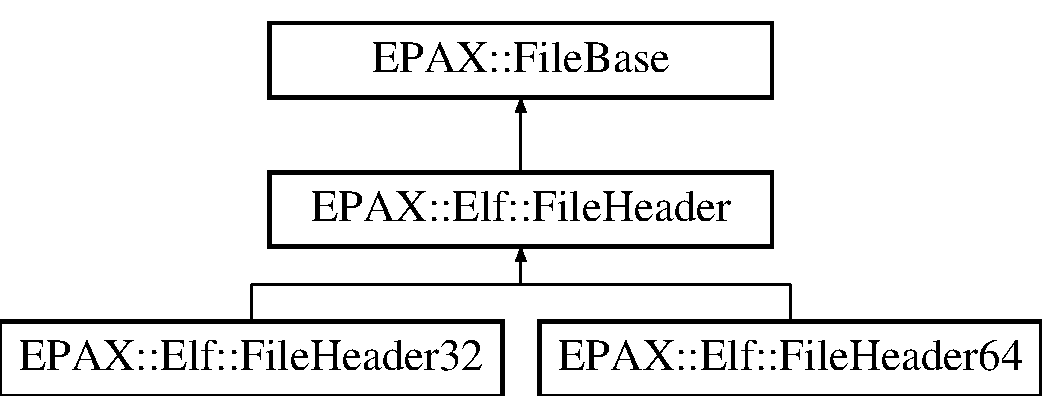
\includegraphics[height=3.000000cm]{class_e_p_a_x_1_1_elf_1_1_file_header}
\end{center}
\end{figure}
\subsection*{\-Public \-Member \-Functions}
\begin{DoxyCompactItemize}
\item 
\hyperlink{class_e_p_a_x_1_1_elf_1_1_file_header_a17ca2c27f8cf31a488aaee78b7314ec0}{\-File\-Header} (\hyperlink{class_e_p_a_x_1_1_base_binary}{\-Base\-Binary} $\ast$b, uint64\-\_\-t o, uint64\-\_\-t s)
\item 
virtual \hyperlink{class_e_p_a_x_1_1_elf_1_1_file_header_a3b9e79ac6ed14a656537ed57f1bb1235}{$\sim$\-File\-Header} ()
\item 
virtual uint64\-\_\-t \hyperlink{class_e_p_a_x_1_1_elf_1_1_file_header_abdf6ca1b4c9bb4e4467ad7467c44730e}{get\-Start\-Addr} ()=0
\item 
virtual bool \hyperlink{class_e_p_a_x_1_1_elf_1_1_file_header_a3ca4cd831fa0b4406c0d4864b659c91c}{verify} ()=0
\item 
virtual bool \hyperlink{class_e_p_a_x_1_1_elf_1_1_file_header_a7213d758b36fccdb80c7c3068155cdee}{is\-A\-R\-M} ()=0
\item 
virtual void \hyperlink{class_e_p_a_x_1_1_elf_1_1_file_header_aeb0eeb9a943fe3382edc7e6b10c3d0d5}{describe} ()=0
\item 
virtual uint32\-\_\-t \hyperlink{class_e_p_a_x_1_1_elf_1_1_file_header_a80f2c4f1a3a4caee7bf6b9b6b7d20d92}{get\-Section\-Count} ()=0
\item 
virtual uint64\-\_\-t \hyperlink{class_e_p_a_x_1_1_elf_1_1_file_header_a465040eb608f51272cb889e4fd0c61f1}{get\-Sec\-Table\-Offset} ()=0
\item 
virtual uint32\-\_\-t \hyperlink{class_e_p_a_x_1_1_elf_1_1_file_header_a52a8d42476216d7946039581f570958f}{get\-Shdr\-Size} ()=0
\item 
virtual uint32\-\_\-t \hyperlink{class_e_p_a_x_1_1_elf_1_1_file_header_aa1d63391748e17afd6ee45c9124d3cc1}{get\-Shdr\-String\-Index} ()=0
\item 
virtual uint32\-\_\-t \hyperlink{class_e_p_a_x_1_1_elf_1_1_file_header_a016aee53224e8350e3b8452b1525aad5}{get\-Segment\-Count} ()=0
\item 
virtual uint64\-\_\-t \hyperlink{class_e_p_a_x_1_1_elf_1_1_file_header_a428d1229cb7324696436d62b8c099239}{get\-Seg\-Table\-Offset} ()=0
\item 
virtual uint32\-\_\-t \hyperlink{class_e_p_a_x_1_1_elf_1_1_file_header_a6d180c7702995629f962abd1cce29e2d}{get\-Phdr\-Size} ()=0
\item 
virtual uint32\-\_\-t \hyperlink{class_e_p_a_x_1_1_elf_1_1_file_header_ae36441d44c2fba9f42709566823b7d08}{get\-File\-Type} ()=0
\end{DoxyCompactItemize}
\subsection*{\-Static \-Protected \-Member \-Functions}
\begin{DoxyCompactItemize}
\item 
static void \hyperlink{class_e_p_a_x_1_1_elf_1_1_file_header_a08520331febff683d5090d71ea762367}{describe\-I\-S\-A} (uint32\-\_\-t ctype)
\end{DoxyCompactItemize}
\subsection*{\-Protected \-Attributes}
\begin{DoxyCompactItemize}
\item 
\hyperlink{_e_p_a_x_common_internal_8hpp_a17755bdd71c02e656c667b16de61dd7b}{rawbyte\-\_\-t} $\ast$ \hyperlink{class_e_p_a_x_1_1_elf_1_1_file_header_a7c2db25209f5833010086dcfe200e67e}{entry}
\end{DoxyCompactItemize}


\subsection{\-Detailed \-Description}


\-Definition at line 101 of file \-Elf\-Binary.\-hpp.



\subsection{\-Constructor \& \-Destructor \-Documentation}
\hypertarget{class_e_p_a_x_1_1_elf_1_1_file_header_a17ca2c27f8cf31a488aaee78b7314ec0}{\index{\-E\-P\-A\-X\-::\-Elf\-::\-File\-Header@{\-E\-P\-A\-X\-::\-Elf\-::\-File\-Header}!\-File\-Header@{\-File\-Header}}
\index{\-File\-Header@{\-File\-Header}!EPAX::Elf::FileHeader@{\-E\-P\-A\-X\-::\-Elf\-::\-File\-Header}}
\subsubsection[{\-File\-Header}]{\setlength{\rightskip}{0pt plus 5cm}{\bf \-E\-P\-A\-X\-::\-Elf\-::\-File\-Header\-::\-File\-Header} (
\begin{DoxyParamCaption}
\item[{{\bf \-Base\-Binary} $\ast$}]{b, }
\item[{uint64\-\_\-t}]{o, }
\item[{uint64\-\_\-t}]{s}
\end{DoxyParamCaption}
)}}\label{class_e_p_a_x_1_1_elf_1_1_file_header_a17ca2c27f8cf31a488aaee78b7314ec0}


\-Definition at line 321 of file \-Elf\-Binary.\-cpp.

\hypertarget{class_e_p_a_x_1_1_elf_1_1_file_header_a3b9e79ac6ed14a656537ed57f1bb1235}{\index{\-E\-P\-A\-X\-::\-Elf\-::\-File\-Header@{\-E\-P\-A\-X\-::\-Elf\-::\-File\-Header}!$\sim$\-File\-Header@{$\sim$\-File\-Header}}
\index{$\sim$\-File\-Header@{$\sim$\-File\-Header}!EPAX::Elf::FileHeader@{\-E\-P\-A\-X\-::\-Elf\-::\-File\-Header}}
\subsubsection[{$\sim$\-File\-Header}]{\setlength{\rightskip}{0pt plus 5cm}{\bf \-E\-P\-A\-X\-::\-Elf\-::\-File\-Header\-::$\sim$\-File\-Header} (
\begin{DoxyParamCaption}
{}
\end{DoxyParamCaption}
)\hspace{0.3cm}{\ttfamily  \mbox{[}virtual\mbox{]}}}}\label{class_e_p_a_x_1_1_elf_1_1_file_header_a3b9e79ac6ed14a656537ed57f1bb1235}


\-Definition at line 327 of file \-Elf\-Binary.\-cpp.



\subsection{\-Member \-Function \-Documentation}
\hypertarget{class_e_p_a_x_1_1_elf_1_1_file_header_aeb0eeb9a943fe3382edc7e6b10c3d0d5}{\index{\-E\-P\-A\-X\-::\-Elf\-::\-File\-Header@{\-E\-P\-A\-X\-::\-Elf\-::\-File\-Header}!describe@{describe}}
\index{describe@{describe}!EPAX::Elf::FileHeader@{\-E\-P\-A\-X\-::\-Elf\-::\-File\-Header}}
\subsubsection[{describe}]{\setlength{\rightskip}{0pt plus 5cm}void {\bf \-E\-P\-A\-X\-::\-Elf\-::\-File\-Header\-::describe} (
\begin{DoxyParamCaption}
{}
\end{DoxyParamCaption}
)\hspace{0.3cm}{\ttfamily  \mbox{[}pure virtual\mbox{]}}}}\label{class_e_p_a_x_1_1_elf_1_1_file_header_aeb0eeb9a943fe3382edc7e6b10c3d0d5}


\-Implemented in \hyperlink{class_e_p_a_x_1_1_elf_1_1_file_header64_a121602d4ffb4f401b59cdb63303fc6c4}{\-E\-P\-A\-X\-::\-Elf\-::\-File\-Header64}, and \hyperlink{class_e_p_a_x_1_1_elf_1_1_file_header32_a85d8cd834a2410f5f51b8a92ca499058}{\-E\-P\-A\-X\-::\-Elf\-::\-File\-Header32}.



\-Definition at line 462 of file \-Elf\-Binary.\-cpp.

\hypertarget{class_e_p_a_x_1_1_elf_1_1_file_header_a08520331febff683d5090d71ea762367}{\index{\-E\-P\-A\-X\-::\-Elf\-::\-File\-Header@{\-E\-P\-A\-X\-::\-Elf\-::\-File\-Header}!describe\-I\-S\-A@{describe\-I\-S\-A}}
\index{describe\-I\-S\-A@{describe\-I\-S\-A}!EPAX::Elf::FileHeader@{\-E\-P\-A\-X\-::\-Elf\-::\-File\-Header}}
\subsubsection[{describe\-I\-S\-A}]{\setlength{\rightskip}{0pt plus 5cm}void {\bf \-E\-P\-A\-X\-::\-Elf\-::\-File\-Header\-::describe\-I\-S\-A} (
\begin{DoxyParamCaption}
\item[{uint32\-\_\-t}]{ctype}
\end{DoxyParamCaption}
)\hspace{0.3cm}{\ttfamily  \mbox{[}static, protected\mbox{]}}}}\label{class_e_p_a_x_1_1_elf_1_1_file_header_a08520331febff683d5090d71ea762367}


\-Definition at line 466 of file \-Elf\-Binary.\-cpp.

\hypertarget{class_e_p_a_x_1_1_elf_1_1_file_header_ae36441d44c2fba9f42709566823b7d08}{\index{\-E\-P\-A\-X\-::\-Elf\-::\-File\-Header@{\-E\-P\-A\-X\-::\-Elf\-::\-File\-Header}!get\-File\-Type@{get\-File\-Type}}
\index{get\-File\-Type@{get\-File\-Type}!EPAX::Elf::FileHeader@{\-E\-P\-A\-X\-::\-Elf\-::\-File\-Header}}
\subsubsection[{get\-File\-Type}]{\setlength{\rightskip}{0pt plus 5cm}virtual uint32\-\_\-t {\bf \-E\-P\-A\-X\-::\-Elf\-::\-File\-Header\-::get\-File\-Type} (
\begin{DoxyParamCaption}
{}
\end{DoxyParamCaption}
)\hspace{0.3cm}{\ttfamily  \mbox{[}pure virtual\mbox{]}}}}\label{class_e_p_a_x_1_1_elf_1_1_file_header_ae36441d44c2fba9f42709566823b7d08}


\-Implemented in \hyperlink{class_e_p_a_x_1_1_elf_1_1_file_header64_a84696d5ac94bd884141c4306025b8ba4}{\-E\-P\-A\-X\-::\-Elf\-::\-File\-Header64}, and \hyperlink{class_e_p_a_x_1_1_elf_1_1_file_header32_af3a51f4aeb49bc78ac18cbb3e8931a5a}{\-E\-P\-A\-X\-::\-Elf\-::\-File\-Header32}.

\hypertarget{class_e_p_a_x_1_1_elf_1_1_file_header_a6d180c7702995629f962abd1cce29e2d}{\index{\-E\-P\-A\-X\-::\-Elf\-::\-File\-Header@{\-E\-P\-A\-X\-::\-Elf\-::\-File\-Header}!get\-Phdr\-Size@{get\-Phdr\-Size}}
\index{get\-Phdr\-Size@{get\-Phdr\-Size}!EPAX::Elf::FileHeader@{\-E\-P\-A\-X\-::\-Elf\-::\-File\-Header}}
\subsubsection[{get\-Phdr\-Size}]{\setlength{\rightskip}{0pt plus 5cm}virtual uint32\-\_\-t {\bf \-E\-P\-A\-X\-::\-Elf\-::\-File\-Header\-::get\-Phdr\-Size} (
\begin{DoxyParamCaption}
{}
\end{DoxyParamCaption}
)\hspace{0.3cm}{\ttfamily  \mbox{[}pure virtual\mbox{]}}}}\label{class_e_p_a_x_1_1_elf_1_1_file_header_a6d180c7702995629f962abd1cce29e2d}


\-Implemented in \hyperlink{class_e_p_a_x_1_1_elf_1_1_file_header64_a389cfa8997b78c7da91bfd980ad61a94}{\-E\-P\-A\-X\-::\-Elf\-::\-File\-Header64}, and \hyperlink{class_e_p_a_x_1_1_elf_1_1_file_header32_ac888b12b41b187273440a028e1b704ca}{\-E\-P\-A\-X\-::\-Elf\-::\-File\-Header32}.

\hypertarget{class_e_p_a_x_1_1_elf_1_1_file_header_a465040eb608f51272cb889e4fd0c61f1}{\index{\-E\-P\-A\-X\-::\-Elf\-::\-File\-Header@{\-E\-P\-A\-X\-::\-Elf\-::\-File\-Header}!get\-Sec\-Table\-Offset@{get\-Sec\-Table\-Offset}}
\index{get\-Sec\-Table\-Offset@{get\-Sec\-Table\-Offset}!EPAX::Elf::FileHeader@{\-E\-P\-A\-X\-::\-Elf\-::\-File\-Header}}
\subsubsection[{get\-Sec\-Table\-Offset}]{\setlength{\rightskip}{0pt plus 5cm}virtual uint64\-\_\-t {\bf \-E\-P\-A\-X\-::\-Elf\-::\-File\-Header\-::get\-Sec\-Table\-Offset} (
\begin{DoxyParamCaption}
{}
\end{DoxyParamCaption}
)\hspace{0.3cm}{\ttfamily  \mbox{[}pure virtual\mbox{]}}}}\label{class_e_p_a_x_1_1_elf_1_1_file_header_a465040eb608f51272cb889e4fd0c61f1}


\-Implemented in \hyperlink{class_e_p_a_x_1_1_elf_1_1_file_header64_ab4bf35526aa8997cdacbe51f401e15a2}{\-E\-P\-A\-X\-::\-Elf\-::\-File\-Header64}, and \hyperlink{class_e_p_a_x_1_1_elf_1_1_file_header32_a8d5c87c8f17e8e6666fde733f9267bae}{\-E\-P\-A\-X\-::\-Elf\-::\-File\-Header32}.

\hypertarget{class_e_p_a_x_1_1_elf_1_1_file_header_a80f2c4f1a3a4caee7bf6b9b6b7d20d92}{\index{\-E\-P\-A\-X\-::\-Elf\-::\-File\-Header@{\-E\-P\-A\-X\-::\-Elf\-::\-File\-Header}!get\-Section\-Count@{get\-Section\-Count}}
\index{get\-Section\-Count@{get\-Section\-Count}!EPAX::Elf::FileHeader@{\-E\-P\-A\-X\-::\-Elf\-::\-File\-Header}}
\subsubsection[{get\-Section\-Count}]{\setlength{\rightskip}{0pt plus 5cm}virtual uint32\-\_\-t {\bf \-E\-P\-A\-X\-::\-Elf\-::\-File\-Header\-::get\-Section\-Count} (
\begin{DoxyParamCaption}
{}
\end{DoxyParamCaption}
)\hspace{0.3cm}{\ttfamily  \mbox{[}pure virtual\mbox{]}}}}\label{class_e_p_a_x_1_1_elf_1_1_file_header_a80f2c4f1a3a4caee7bf6b9b6b7d20d92}


\-Implemented in \hyperlink{class_e_p_a_x_1_1_elf_1_1_file_header64_a525b2d31bb8ad212c197172006cd8b90}{\-E\-P\-A\-X\-::\-Elf\-::\-File\-Header64}, and \hyperlink{class_e_p_a_x_1_1_elf_1_1_file_header32_ac1dd93429930f0a1f5991cb6270a383e}{\-E\-P\-A\-X\-::\-Elf\-::\-File\-Header32}.

\hypertarget{class_e_p_a_x_1_1_elf_1_1_file_header_a016aee53224e8350e3b8452b1525aad5}{\index{\-E\-P\-A\-X\-::\-Elf\-::\-File\-Header@{\-E\-P\-A\-X\-::\-Elf\-::\-File\-Header}!get\-Segment\-Count@{get\-Segment\-Count}}
\index{get\-Segment\-Count@{get\-Segment\-Count}!EPAX::Elf::FileHeader@{\-E\-P\-A\-X\-::\-Elf\-::\-File\-Header}}
\subsubsection[{get\-Segment\-Count}]{\setlength{\rightskip}{0pt plus 5cm}virtual uint32\-\_\-t {\bf \-E\-P\-A\-X\-::\-Elf\-::\-File\-Header\-::get\-Segment\-Count} (
\begin{DoxyParamCaption}
{}
\end{DoxyParamCaption}
)\hspace{0.3cm}{\ttfamily  \mbox{[}pure virtual\mbox{]}}}}\label{class_e_p_a_x_1_1_elf_1_1_file_header_a016aee53224e8350e3b8452b1525aad5}


\-Implemented in \hyperlink{class_e_p_a_x_1_1_elf_1_1_file_header64_af0e3dc9b8ae0832bd9a24d2c72e09011}{\-E\-P\-A\-X\-::\-Elf\-::\-File\-Header64}, and \hyperlink{class_e_p_a_x_1_1_elf_1_1_file_header32_ac38fc67d4991960a64e43418355847dc}{\-E\-P\-A\-X\-::\-Elf\-::\-File\-Header32}.

\hypertarget{class_e_p_a_x_1_1_elf_1_1_file_header_a428d1229cb7324696436d62b8c099239}{\index{\-E\-P\-A\-X\-::\-Elf\-::\-File\-Header@{\-E\-P\-A\-X\-::\-Elf\-::\-File\-Header}!get\-Seg\-Table\-Offset@{get\-Seg\-Table\-Offset}}
\index{get\-Seg\-Table\-Offset@{get\-Seg\-Table\-Offset}!EPAX::Elf::FileHeader@{\-E\-P\-A\-X\-::\-Elf\-::\-File\-Header}}
\subsubsection[{get\-Seg\-Table\-Offset}]{\setlength{\rightskip}{0pt plus 5cm}virtual uint64\-\_\-t {\bf \-E\-P\-A\-X\-::\-Elf\-::\-File\-Header\-::get\-Seg\-Table\-Offset} (
\begin{DoxyParamCaption}
{}
\end{DoxyParamCaption}
)\hspace{0.3cm}{\ttfamily  \mbox{[}pure virtual\mbox{]}}}}\label{class_e_p_a_x_1_1_elf_1_1_file_header_a428d1229cb7324696436d62b8c099239}


\-Implemented in \hyperlink{class_e_p_a_x_1_1_elf_1_1_file_header64_ad05c5e3abb06032413b058f5db1f3f9c}{\-E\-P\-A\-X\-::\-Elf\-::\-File\-Header64}, and \hyperlink{class_e_p_a_x_1_1_elf_1_1_file_header32_a726775497585b20e7b5bfcf523492824}{\-E\-P\-A\-X\-::\-Elf\-::\-File\-Header32}.

\hypertarget{class_e_p_a_x_1_1_elf_1_1_file_header_a52a8d42476216d7946039581f570958f}{\index{\-E\-P\-A\-X\-::\-Elf\-::\-File\-Header@{\-E\-P\-A\-X\-::\-Elf\-::\-File\-Header}!get\-Shdr\-Size@{get\-Shdr\-Size}}
\index{get\-Shdr\-Size@{get\-Shdr\-Size}!EPAX::Elf::FileHeader@{\-E\-P\-A\-X\-::\-Elf\-::\-File\-Header}}
\subsubsection[{get\-Shdr\-Size}]{\setlength{\rightskip}{0pt plus 5cm}virtual uint32\-\_\-t {\bf \-E\-P\-A\-X\-::\-Elf\-::\-File\-Header\-::get\-Shdr\-Size} (
\begin{DoxyParamCaption}
{}
\end{DoxyParamCaption}
)\hspace{0.3cm}{\ttfamily  \mbox{[}pure virtual\mbox{]}}}}\label{class_e_p_a_x_1_1_elf_1_1_file_header_a52a8d42476216d7946039581f570958f}


\-Implemented in \hyperlink{class_e_p_a_x_1_1_elf_1_1_file_header64_ad4c76f6ef875eccd6e453c61736d7e40}{\-E\-P\-A\-X\-::\-Elf\-::\-File\-Header64}, and \hyperlink{class_e_p_a_x_1_1_elf_1_1_file_header32_a0ed67a18b9abbe58cd2527e4c67d04e6}{\-E\-P\-A\-X\-::\-Elf\-::\-File\-Header32}.

\hypertarget{class_e_p_a_x_1_1_elf_1_1_file_header_aa1d63391748e17afd6ee45c9124d3cc1}{\index{\-E\-P\-A\-X\-::\-Elf\-::\-File\-Header@{\-E\-P\-A\-X\-::\-Elf\-::\-File\-Header}!get\-Shdr\-String\-Index@{get\-Shdr\-String\-Index}}
\index{get\-Shdr\-String\-Index@{get\-Shdr\-String\-Index}!EPAX::Elf::FileHeader@{\-E\-P\-A\-X\-::\-Elf\-::\-File\-Header}}
\subsubsection[{get\-Shdr\-String\-Index}]{\setlength{\rightskip}{0pt plus 5cm}virtual uint32\-\_\-t {\bf \-E\-P\-A\-X\-::\-Elf\-::\-File\-Header\-::get\-Shdr\-String\-Index} (
\begin{DoxyParamCaption}
{}
\end{DoxyParamCaption}
)\hspace{0.3cm}{\ttfamily  \mbox{[}pure virtual\mbox{]}}}}\label{class_e_p_a_x_1_1_elf_1_1_file_header_aa1d63391748e17afd6ee45c9124d3cc1}


\-Implemented in \hyperlink{class_e_p_a_x_1_1_elf_1_1_file_header64_a1e776b6ef8858287951a39a15626a6da}{\-E\-P\-A\-X\-::\-Elf\-::\-File\-Header64}, and \hyperlink{class_e_p_a_x_1_1_elf_1_1_file_header32_a06e25aa5ff7df704d070abaa8ba3c1aa}{\-E\-P\-A\-X\-::\-Elf\-::\-File\-Header32}.

\hypertarget{class_e_p_a_x_1_1_elf_1_1_file_header_abdf6ca1b4c9bb4e4467ad7467c44730e}{\index{\-E\-P\-A\-X\-::\-Elf\-::\-File\-Header@{\-E\-P\-A\-X\-::\-Elf\-::\-File\-Header}!get\-Start\-Addr@{get\-Start\-Addr}}
\index{get\-Start\-Addr@{get\-Start\-Addr}!EPAX::Elf::FileHeader@{\-E\-P\-A\-X\-::\-Elf\-::\-File\-Header}}
\subsubsection[{get\-Start\-Addr}]{\setlength{\rightskip}{0pt plus 5cm}virtual uint64\-\_\-t {\bf \-E\-P\-A\-X\-::\-Elf\-::\-File\-Header\-::get\-Start\-Addr} (
\begin{DoxyParamCaption}
{}
\end{DoxyParamCaption}
)\hspace{0.3cm}{\ttfamily  \mbox{[}pure virtual\mbox{]}}}}\label{class_e_p_a_x_1_1_elf_1_1_file_header_abdf6ca1b4c9bb4e4467ad7467c44730e}


\-Implemented in \hyperlink{class_e_p_a_x_1_1_elf_1_1_file_header64_a0d5fb6bb80415565bec58de93526a2ea}{\-E\-P\-A\-X\-::\-Elf\-::\-File\-Header64}, and \hyperlink{class_e_p_a_x_1_1_elf_1_1_file_header32_ab8a7bf656d86963f9324b2c3686090e1}{\-E\-P\-A\-X\-::\-Elf\-::\-File\-Header32}.

\hypertarget{class_e_p_a_x_1_1_elf_1_1_file_header_a7213d758b36fccdb80c7c3068155cdee}{\index{\-E\-P\-A\-X\-::\-Elf\-::\-File\-Header@{\-E\-P\-A\-X\-::\-Elf\-::\-File\-Header}!is\-A\-R\-M@{is\-A\-R\-M}}
\index{is\-A\-R\-M@{is\-A\-R\-M}!EPAX::Elf::FileHeader@{\-E\-P\-A\-X\-::\-Elf\-::\-File\-Header}}
\subsubsection[{is\-A\-R\-M}]{\setlength{\rightskip}{0pt plus 5cm}virtual bool {\bf \-E\-P\-A\-X\-::\-Elf\-::\-File\-Header\-::is\-A\-R\-M} (
\begin{DoxyParamCaption}
{}
\end{DoxyParamCaption}
)\hspace{0.3cm}{\ttfamily  \mbox{[}pure virtual\mbox{]}}}}\label{class_e_p_a_x_1_1_elf_1_1_file_header_a7213d758b36fccdb80c7c3068155cdee}


\-Implemented in \hyperlink{class_e_p_a_x_1_1_elf_1_1_file_header64_a6d992697b0003b0c63f9e9b6271de94a}{\-E\-P\-A\-X\-::\-Elf\-::\-File\-Header64}, and \hyperlink{class_e_p_a_x_1_1_elf_1_1_file_header32_af3918b11e74da5f92738df8c70c34258}{\-E\-P\-A\-X\-::\-Elf\-::\-File\-Header32}.

\hypertarget{class_e_p_a_x_1_1_elf_1_1_file_header_a3ca4cd831fa0b4406c0d4864b659c91c}{\index{\-E\-P\-A\-X\-::\-Elf\-::\-File\-Header@{\-E\-P\-A\-X\-::\-Elf\-::\-File\-Header}!verify@{verify}}
\index{verify@{verify}!EPAX::Elf::FileHeader@{\-E\-P\-A\-X\-::\-Elf\-::\-File\-Header}}
\subsubsection[{verify}]{\setlength{\rightskip}{0pt plus 5cm}virtual bool {\bf \-E\-P\-A\-X\-::\-Elf\-::\-File\-Header\-::verify} (
\begin{DoxyParamCaption}
{}
\end{DoxyParamCaption}
)\hspace{0.3cm}{\ttfamily  \mbox{[}pure virtual\mbox{]}}}}\label{class_e_p_a_x_1_1_elf_1_1_file_header_a3ca4cd831fa0b4406c0d4864b659c91c}


\-Implemented in \hyperlink{class_e_p_a_x_1_1_elf_1_1_file_header64_a6a94d18eaee683c6bbe05f3b57f08efc}{\-E\-P\-A\-X\-::\-Elf\-::\-File\-Header64}, and \hyperlink{class_e_p_a_x_1_1_elf_1_1_file_header32_a39dbffddc4e4503da772ebcd66c9c760}{\-E\-P\-A\-X\-::\-Elf\-::\-File\-Header32}.



\subsection{\-Member \-Data \-Documentation}
\hypertarget{class_e_p_a_x_1_1_elf_1_1_file_header_a7c2db25209f5833010086dcfe200e67e}{\index{\-E\-P\-A\-X\-::\-Elf\-::\-File\-Header@{\-E\-P\-A\-X\-::\-Elf\-::\-File\-Header}!entry@{entry}}
\index{entry@{entry}!EPAX::Elf::FileHeader@{\-E\-P\-A\-X\-::\-Elf\-::\-File\-Header}}
\subsubsection[{entry}]{\setlength{\rightskip}{0pt plus 5cm}{\bf rawbyte\-\_\-t}$\ast$ {\bf \-E\-P\-A\-X\-::\-Elf\-::\-File\-Header\-::entry}\hspace{0.3cm}{\ttfamily  \mbox{[}protected\mbox{]}}}}\label{class_e_p_a_x_1_1_elf_1_1_file_header_a7c2db25209f5833010086dcfe200e67e}


\-Definition at line 103 of file \-Elf\-Binary.\-hpp.



\-The documentation for this class was generated from the following files\-:\begin{DoxyCompactItemize}
\item 
\hyperlink{_elf_binary_8hpp}{\-Elf\-Binary.\-hpp}\item 
\hyperlink{_elf_binary_8cpp}{\-Elf\-Binary.\-cpp}\end{DoxyCompactItemize}

\hypertarget{class_e_p_a_x_1_1_elf_1_1_file_header32}{\section{\-E\-P\-A\-X\-:\-:\-Elf\-:\-:\-File\-Header32 \-Class \-Reference}
\label{class_e_p_a_x_1_1_elf_1_1_file_header32}\index{\-E\-P\-A\-X\-::\-Elf\-::\-File\-Header32@{\-E\-P\-A\-X\-::\-Elf\-::\-File\-Header32}}
}


{\ttfamily \#include $<$\-Elf\-Binary.\-hpp$>$}

\-Inheritance diagram for \-E\-P\-A\-X\-:\-:\-Elf\-:\-:\-File\-Header32\-:\begin{figure}[H]
\begin{center}
\leavevmode
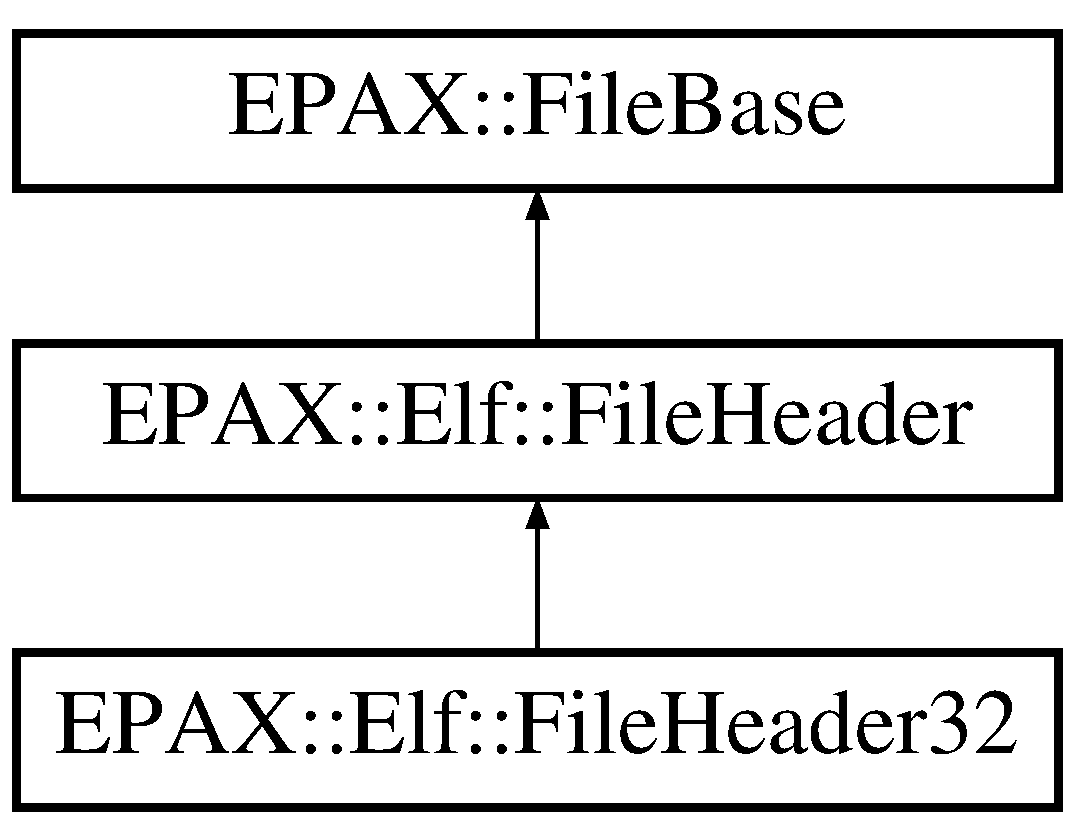
\includegraphics[height=3.000000cm]{class_e_p_a_x_1_1_elf_1_1_file_header32}
\end{center}
\end{figure}
\subsection*{\-Public \-Member \-Functions}
\begin{DoxyCompactItemize}
\item 
\hyperlink{class_e_p_a_x_1_1_elf_1_1_file_header32_abffac5321d1935c5a829715f5d4dbd63}{\-File\-Header32} (\hyperlink{class_e_p_a_x_1_1_base_binary}{\-Base\-Binary} $\ast$b, uint64\-\_\-t o)
\item 
virtual \hyperlink{class_e_p_a_x_1_1_elf_1_1_file_header32_aa3b5df3c225b2aa6b08a6378e16677c1}{$\sim$\-File\-Header32} ()
\item 
uint64\-\_\-t \hyperlink{class_e_p_a_x_1_1_elf_1_1_file_header32_ab8a7bf656d86963f9324b2c3686090e1}{get\-Start\-Addr} ()
\item 
bool \hyperlink{class_e_p_a_x_1_1_elf_1_1_file_header32_a39dbffddc4e4503da772ebcd66c9c760}{verify} ()
\item 
bool \hyperlink{class_e_p_a_x_1_1_elf_1_1_file_header32_af3918b11e74da5f92738df8c70c34258}{is\-A\-R\-M} ()
\item 
void \hyperlink{class_e_p_a_x_1_1_elf_1_1_file_header32_a85d8cd834a2410f5f51b8a92ca499058}{describe} ()
\item 
uint32\-\_\-t \hyperlink{class_e_p_a_x_1_1_elf_1_1_file_header32_ac1dd93429930f0a1f5991cb6270a383e}{get\-Section\-Count} ()
\item 
uint64\-\_\-t \hyperlink{class_e_p_a_x_1_1_elf_1_1_file_header32_a8d5c87c8f17e8e6666fde733f9267bae}{get\-Sec\-Table\-Offset} ()
\item 
uint32\-\_\-t \hyperlink{class_e_p_a_x_1_1_elf_1_1_file_header32_a0ed67a18b9abbe58cd2527e4c67d04e6}{get\-Shdr\-Size} ()
\item 
uint32\-\_\-t \hyperlink{class_e_p_a_x_1_1_elf_1_1_file_header32_a06e25aa5ff7df704d070abaa8ba3c1aa}{get\-Shdr\-String\-Index} ()
\item 
uint32\-\_\-t \hyperlink{class_e_p_a_x_1_1_elf_1_1_file_header32_ac38fc67d4991960a64e43418355847dc}{get\-Segment\-Count} ()
\item 
uint64\-\_\-t \hyperlink{class_e_p_a_x_1_1_elf_1_1_file_header32_a726775497585b20e7b5bfcf523492824}{get\-Seg\-Table\-Offset} ()
\item 
uint32\-\_\-t \hyperlink{class_e_p_a_x_1_1_elf_1_1_file_header32_ac888b12b41b187273440a028e1b704ca}{get\-Phdr\-Size} ()
\item 
uint32\-\_\-t \hyperlink{class_e_p_a_x_1_1_elf_1_1_file_header32_af3a51f4aeb49bc78ac18cbb3e8931a5a}{get\-File\-Type} ()
\end{DoxyCompactItemize}


\subsection{\-Detailed \-Description}


\-Definition at line 127 of file \-Elf\-Binary.\-hpp.



\subsection{\-Constructor \& \-Destructor \-Documentation}
\hypertarget{class_e_p_a_x_1_1_elf_1_1_file_header32_abffac5321d1935c5a829715f5d4dbd63}{\index{\-E\-P\-A\-X\-::\-Elf\-::\-File\-Header32@{\-E\-P\-A\-X\-::\-Elf\-::\-File\-Header32}!\-File\-Header32@{\-File\-Header32}}
\index{\-File\-Header32@{\-File\-Header32}!EPAX::Elf::FileHeader32@{\-E\-P\-A\-X\-::\-Elf\-::\-File\-Header32}}
\subsubsection[{\-File\-Header32}]{\setlength{\rightskip}{0pt plus 5cm}{\bf \-E\-P\-A\-X\-::\-Elf\-::\-File\-Header32\-::\-File\-Header32} (
\begin{DoxyParamCaption}
\item[{{\bf \-Base\-Binary} $\ast$}]{b, }
\item[{uint64\-\_\-t}]{o}
\end{DoxyParamCaption}
)}}\label{class_e_p_a_x_1_1_elf_1_1_file_header32_abffac5321d1935c5a829715f5d4dbd63}


\-Definition at line 397 of file \-Elf\-Binary.\-cpp.

\hypertarget{class_e_p_a_x_1_1_elf_1_1_file_header32_aa3b5df3c225b2aa6b08a6378e16677c1}{\index{\-E\-P\-A\-X\-::\-Elf\-::\-File\-Header32@{\-E\-P\-A\-X\-::\-Elf\-::\-File\-Header32}!$\sim$\-File\-Header32@{$\sim$\-File\-Header32}}
\index{$\sim$\-File\-Header32@{$\sim$\-File\-Header32}!EPAX::Elf::FileHeader32@{\-E\-P\-A\-X\-::\-Elf\-::\-File\-Header32}}
\subsubsection[{$\sim$\-File\-Header32}]{\setlength{\rightskip}{0pt plus 5cm}virtual {\bf \-E\-P\-A\-X\-::\-Elf\-::\-File\-Header32\-::$\sim$\-File\-Header32} (
\begin{DoxyParamCaption}
{}
\end{DoxyParamCaption}
)\hspace{0.3cm}{\ttfamily  \mbox{[}inline, virtual\mbox{]}}}}\label{class_e_p_a_x_1_1_elf_1_1_file_header32_aa3b5df3c225b2aa6b08a6378e16677c1}


\-Definition at line 131 of file \-Elf\-Binary.\-hpp.



\subsection{\-Member \-Function \-Documentation}
\hypertarget{class_e_p_a_x_1_1_elf_1_1_file_header32_a85d8cd834a2410f5f51b8a92ca499058}{\index{\-E\-P\-A\-X\-::\-Elf\-::\-File\-Header32@{\-E\-P\-A\-X\-::\-Elf\-::\-File\-Header32}!describe@{describe}}
\index{describe@{describe}!EPAX::Elf::FileHeader32@{\-E\-P\-A\-X\-::\-Elf\-::\-File\-Header32}}
\subsubsection[{describe}]{\setlength{\rightskip}{0pt plus 5cm}void {\bf \-E\-P\-A\-X\-::\-Elf\-::\-File\-Header32\-::describe} (
\begin{DoxyParamCaption}
{}
\end{DoxyParamCaption}
)\hspace{0.3cm}{\ttfamily  \mbox{[}virtual\mbox{]}}}}\label{class_e_p_a_x_1_1_elf_1_1_file_header32_a85d8cd834a2410f5f51b8a92ca499058}


\-Implements \hyperlink{class_e_p_a_x_1_1_elf_1_1_file_header_aeb0eeb9a943fe3382edc7e6b10c3d0d5}{\-E\-P\-A\-X\-::\-Elf\-::\-File\-Header}.



\-Definition at line 484 of file \-Elf\-Binary.\-cpp.

\hypertarget{class_e_p_a_x_1_1_elf_1_1_file_header32_af3a51f4aeb49bc78ac18cbb3e8931a5a}{\index{\-E\-P\-A\-X\-::\-Elf\-::\-File\-Header32@{\-E\-P\-A\-X\-::\-Elf\-::\-File\-Header32}!get\-File\-Type@{get\-File\-Type}}
\index{get\-File\-Type@{get\-File\-Type}!EPAX::Elf::FileHeader32@{\-E\-P\-A\-X\-::\-Elf\-::\-File\-Header32}}
\subsubsection[{get\-File\-Type}]{\setlength{\rightskip}{0pt plus 5cm}uint32\-\_\-t {\bf \-E\-P\-A\-X\-::\-Elf\-::\-File\-Header32\-::get\-File\-Type} (
\begin{DoxyParamCaption}
{}
\end{DoxyParamCaption}
)\hspace{0.3cm}{\ttfamily  \mbox{[}virtual\mbox{]}}}}\label{class_e_p_a_x_1_1_elf_1_1_file_header32_af3a51f4aeb49bc78ac18cbb3e8931a5a}


\-Implements \hyperlink{class_e_p_a_x_1_1_elf_1_1_file_header_ae36441d44c2fba9f42709566823b7d08}{\-E\-P\-A\-X\-::\-Elf\-::\-File\-Header}.



\-Definition at line 389 of file \-Elf\-Binary.\-cpp.

\hypertarget{class_e_p_a_x_1_1_elf_1_1_file_header32_ac888b12b41b187273440a028e1b704ca}{\index{\-E\-P\-A\-X\-::\-Elf\-::\-File\-Header32@{\-E\-P\-A\-X\-::\-Elf\-::\-File\-Header32}!get\-Phdr\-Size@{get\-Phdr\-Size}}
\index{get\-Phdr\-Size@{get\-Phdr\-Size}!EPAX::Elf::FileHeader32@{\-E\-P\-A\-X\-::\-Elf\-::\-File\-Header32}}
\subsubsection[{get\-Phdr\-Size}]{\setlength{\rightskip}{0pt plus 5cm}uint32\-\_\-t {\bf \-E\-P\-A\-X\-::\-Elf\-::\-File\-Header32\-::get\-Phdr\-Size} (
\begin{DoxyParamCaption}
{}
\end{DoxyParamCaption}
)\hspace{0.3cm}{\ttfamily  \mbox{[}virtual\mbox{]}}}}\label{class_e_p_a_x_1_1_elf_1_1_file_header32_ac888b12b41b187273440a028e1b704ca}


\-Implements \hyperlink{class_e_p_a_x_1_1_elf_1_1_file_header_a6d180c7702995629f962abd1cce29e2d}{\-E\-P\-A\-X\-::\-Elf\-::\-File\-Header}.



\-Definition at line 357 of file \-Elf\-Binary.\-cpp.

\hypertarget{class_e_p_a_x_1_1_elf_1_1_file_header32_a8d5c87c8f17e8e6666fde733f9267bae}{\index{\-E\-P\-A\-X\-::\-Elf\-::\-File\-Header32@{\-E\-P\-A\-X\-::\-Elf\-::\-File\-Header32}!get\-Sec\-Table\-Offset@{get\-Sec\-Table\-Offset}}
\index{get\-Sec\-Table\-Offset@{get\-Sec\-Table\-Offset}!EPAX::Elf::FileHeader32@{\-E\-P\-A\-X\-::\-Elf\-::\-File\-Header32}}
\subsubsection[{get\-Sec\-Table\-Offset}]{\setlength{\rightskip}{0pt plus 5cm}uint64\-\_\-t {\bf \-E\-P\-A\-X\-::\-Elf\-::\-File\-Header32\-::get\-Sec\-Table\-Offset} (
\begin{DoxyParamCaption}
{}
\end{DoxyParamCaption}
)\hspace{0.3cm}{\ttfamily  \mbox{[}virtual\mbox{]}}}}\label{class_e_p_a_x_1_1_elf_1_1_file_header32_a8d5c87c8f17e8e6666fde733f9267bae}


\-Implements \hyperlink{class_e_p_a_x_1_1_elf_1_1_file_header_a465040eb608f51272cb889e4fd0c61f1}{\-E\-P\-A\-X\-::\-Elf\-::\-File\-Header}.



\-Definition at line 333 of file \-Elf\-Binary.\-cpp.

\hypertarget{class_e_p_a_x_1_1_elf_1_1_file_header32_ac1dd93429930f0a1f5991cb6270a383e}{\index{\-E\-P\-A\-X\-::\-Elf\-::\-File\-Header32@{\-E\-P\-A\-X\-::\-Elf\-::\-File\-Header32}!get\-Section\-Count@{get\-Section\-Count}}
\index{get\-Section\-Count@{get\-Section\-Count}!EPAX::Elf::FileHeader32@{\-E\-P\-A\-X\-::\-Elf\-::\-File\-Header32}}
\subsubsection[{get\-Section\-Count}]{\setlength{\rightskip}{0pt plus 5cm}uint32\-\_\-t {\bf \-E\-P\-A\-X\-::\-Elf\-::\-File\-Header32\-::get\-Section\-Count} (
\begin{DoxyParamCaption}
{}
\end{DoxyParamCaption}
)\hspace{0.3cm}{\ttfamily  \mbox{[}virtual\mbox{]}}}}\label{class_e_p_a_x_1_1_elf_1_1_file_header32_ac1dd93429930f0a1f5991cb6270a383e}


\-Implements \hyperlink{class_e_p_a_x_1_1_elf_1_1_file_header_a80f2c4f1a3a4caee7bf6b9b6b7d20d92}{\-E\-P\-A\-X\-::\-Elf\-::\-File\-Header}.



\-Definition at line 373 of file \-Elf\-Binary.\-cpp.

\hypertarget{class_e_p_a_x_1_1_elf_1_1_file_header32_ac38fc67d4991960a64e43418355847dc}{\index{\-E\-P\-A\-X\-::\-Elf\-::\-File\-Header32@{\-E\-P\-A\-X\-::\-Elf\-::\-File\-Header32}!get\-Segment\-Count@{get\-Segment\-Count}}
\index{get\-Segment\-Count@{get\-Segment\-Count}!EPAX::Elf::FileHeader32@{\-E\-P\-A\-X\-::\-Elf\-::\-File\-Header32}}
\subsubsection[{get\-Segment\-Count}]{\setlength{\rightskip}{0pt plus 5cm}uint32\-\_\-t {\bf \-E\-P\-A\-X\-::\-Elf\-::\-File\-Header32\-::get\-Segment\-Count} (
\begin{DoxyParamCaption}
{}
\end{DoxyParamCaption}
)\hspace{0.3cm}{\ttfamily  \mbox{[}virtual\mbox{]}}}}\label{class_e_p_a_x_1_1_elf_1_1_file_header32_ac38fc67d4991960a64e43418355847dc}


\-Implements \hyperlink{class_e_p_a_x_1_1_elf_1_1_file_header_a016aee53224e8350e3b8452b1525aad5}{\-E\-P\-A\-X\-::\-Elf\-::\-File\-Header}.



\-Definition at line 381 of file \-Elf\-Binary.\-cpp.

\hypertarget{class_e_p_a_x_1_1_elf_1_1_file_header32_a726775497585b20e7b5bfcf523492824}{\index{\-E\-P\-A\-X\-::\-Elf\-::\-File\-Header32@{\-E\-P\-A\-X\-::\-Elf\-::\-File\-Header32}!get\-Seg\-Table\-Offset@{get\-Seg\-Table\-Offset}}
\index{get\-Seg\-Table\-Offset@{get\-Seg\-Table\-Offset}!EPAX::Elf::FileHeader32@{\-E\-P\-A\-X\-::\-Elf\-::\-File\-Header32}}
\subsubsection[{get\-Seg\-Table\-Offset}]{\setlength{\rightskip}{0pt plus 5cm}uint64\-\_\-t {\bf \-E\-P\-A\-X\-::\-Elf\-::\-File\-Header32\-::get\-Seg\-Table\-Offset} (
\begin{DoxyParamCaption}
{}
\end{DoxyParamCaption}
)\hspace{0.3cm}{\ttfamily  \mbox{[}virtual\mbox{]}}}}\label{class_e_p_a_x_1_1_elf_1_1_file_header32_a726775497585b20e7b5bfcf523492824}


\-Implements \hyperlink{class_e_p_a_x_1_1_elf_1_1_file_header_a428d1229cb7324696436d62b8c099239}{\-E\-P\-A\-X\-::\-Elf\-::\-File\-Header}.



\-Definition at line 349 of file \-Elf\-Binary.\-cpp.

\hypertarget{class_e_p_a_x_1_1_elf_1_1_file_header32_a0ed67a18b9abbe58cd2527e4c67d04e6}{\index{\-E\-P\-A\-X\-::\-Elf\-::\-File\-Header32@{\-E\-P\-A\-X\-::\-Elf\-::\-File\-Header32}!get\-Shdr\-Size@{get\-Shdr\-Size}}
\index{get\-Shdr\-Size@{get\-Shdr\-Size}!EPAX::Elf::FileHeader32@{\-E\-P\-A\-X\-::\-Elf\-::\-File\-Header32}}
\subsubsection[{get\-Shdr\-Size}]{\setlength{\rightskip}{0pt plus 5cm}uint32\-\_\-t {\bf \-E\-P\-A\-X\-::\-Elf\-::\-File\-Header32\-::get\-Shdr\-Size} (
\begin{DoxyParamCaption}
{}
\end{DoxyParamCaption}
)\hspace{0.3cm}{\ttfamily  \mbox{[}virtual\mbox{]}}}}\label{class_e_p_a_x_1_1_elf_1_1_file_header32_a0ed67a18b9abbe58cd2527e4c67d04e6}


\-Implements \hyperlink{class_e_p_a_x_1_1_elf_1_1_file_header_a52a8d42476216d7946039581f570958f}{\-E\-P\-A\-X\-::\-Elf\-::\-File\-Header}.



\-Definition at line 341 of file \-Elf\-Binary.\-cpp.

\hypertarget{class_e_p_a_x_1_1_elf_1_1_file_header32_a06e25aa5ff7df704d070abaa8ba3c1aa}{\index{\-E\-P\-A\-X\-::\-Elf\-::\-File\-Header32@{\-E\-P\-A\-X\-::\-Elf\-::\-File\-Header32}!get\-Shdr\-String\-Index@{get\-Shdr\-String\-Index}}
\index{get\-Shdr\-String\-Index@{get\-Shdr\-String\-Index}!EPAX::Elf::FileHeader32@{\-E\-P\-A\-X\-::\-Elf\-::\-File\-Header32}}
\subsubsection[{get\-Shdr\-String\-Index}]{\setlength{\rightskip}{0pt plus 5cm}uint32\-\_\-t {\bf \-E\-P\-A\-X\-::\-Elf\-::\-File\-Header32\-::get\-Shdr\-String\-Index} (
\begin{DoxyParamCaption}
{}
\end{DoxyParamCaption}
)\hspace{0.3cm}{\ttfamily  \mbox{[}virtual\mbox{]}}}}\label{class_e_p_a_x_1_1_elf_1_1_file_header32_a06e25aa5ff7df704d070abaa8ba3c1aa}


\-Implements \hyperlink{class_e_p_a_x_1_1_elf_1_1_file_header_aa1d63391748e17afd6ee45c9124d3cc1}{\-E\-P\-A\-X\-::\-Elf\-::\-File\-Header}.



\-Definition at line 365 of file \-Elf\-Binary.\-cpp.

\hypertarget{class_e_p_a_x_1_1_elf_1_1_file_header32_ab8a7bf656d86963f9324b2c3686090e1}{\index{\-E\-P\-A\-X\-::\-Elf\-::\-File\-Header32@{\-E\-P\-A\-X\-::\-Elf\-::\-File\-Header32}!get\-Start\-Addr@{get\-Start\-Addr}}
\index{get\-Start\-Addr@{get\-Start\-Addr}!EPAX::Elf::FileHeader32@{\-E\-P\-A\-X\-::\-Elf\-::\-File\-Header32}}
\subsubsection[{get\-Start\-Addr}]{\setlength{\rightskip}{0pt plus 5cm}uint64\-\_\-t {\bf \-E\-P\-A\-X\-::\-Elf\-::\-File\-Header32\-::get\-Start\-Addr} (
\begin{DoxyParamCaption}
{}
\end{DoxyParamCaption}
)\hspace{0.3cm}{\ttfamily  \mbox{[}virtual\mbox{]}}}}\label{class_e_p_a_x_1_1_elf_1_1_file_header32_ab8a7bf656d86963f9324b2c3686090e1}


\-Implements \hyperlink{class_e_p_a_x_1_1_elf_1_1_file_header_abdf6ca1b4c9bb4e4467ad7467c44730e}{\-E\-P\-A\-X\-::\-Elf\-::\-File\-Header}.



\-Definition at line 411 of file \-Elf\-Binary.\-cpp.

\hypertarget{class_e_p_a_x_1_1_elf_1_1_file_header32_af3918b11e74da5f92738df8c70c34258}{\index{\-E\-P\-A\-X\-::\-Elf\-::\-File\-Header32@{\-E\-P\-A\-X\-::\-Elf\-::\-File\-Header32}!is\-A\-R\-M@{is\-A\-R\-M}}
\index{is\-A\-R\-M@{is\-A\-R\-M}!EPAX::Elf::FileHeader32@{\-E\-P\-A\-X\-::\-Elf\-::\-File\-Header32}}
\subsubsection[{is\-A\-R\-M}]{\setlength{\rightskip}{0pt plus 5cm}bool {\bf \-E\-P\-A\-X\-::\-Elf\-::\-File\-Header32\-::is\-A\-R\-M} (
\begin{DoxyParamCaption}
{}
\end{DoxyParamCaption}
)\hspace{0.3cm}{\ttfamily  \mbox{[}virtual\mbox{]}}}}\label{class_e_p_a_x_1_1_elf_1_1_file_header32_af3918b11e74da5f92738df8c70c34258}


\-Implements \hyperlink{class_e_p_a_x_1_1_elf_1_1_file_header_a7213d758b36fccdb80c7c3068155cdee}{\-E\-P\-A\-X\-::\-Elf\-::\-File\-Header}.



\-Definition at line 447 of file \-Elf\-Binary.\-cpp.

\hypertarget{class_e_p_a_x_1_1_elf_1_1_file_header32_a39dbffddc4e4503da772ebcd66c9c760}{\index{\-E\-P\-A\-X\-::\-Elf\-::\-File\-Header32@{\-E\-P\-A\-X\-::\-Elf\-::\-File\-Header32}!verify@{verify}}
\index{verify@{verify}!EPAX::Elf::FileHeader32@{\-E\-P\-A\-X\-::\-Elf\-::\-File\-Header32}}
\subsubsection[{verify}]{\setlength{\rightskip}{0pt plus 5cm}bool {\bf \-E\-P\-A\-X\-::\-Elf\-::\-File\-Header32\-::verify} (
\begin{DoxyParamCaption}
{}
\end{DoxyParamCaption}
)\hspace{0.3cm}{\ttfamily  \mbox{[}virtual\mbox{]}}}}\label{class_e_p_a_x_1_1_elf_1_1_file_header32_a39dbffddc4e4503da772ebcd66c9c760}


\-Implements \hyperlink{class_e_p_a_x_1_1_elf_1_1_file_header_a3ca4cd831fa0b4406c0d4864b659c91c}{\-E\-P\-A\-X\-::\-Elf\-::\-File\-Header}.



\-Definition at line 419 of file \-Elf\-Binary.\-cpp.



\-The documentation for this class was generated from the following files\-:\begin{DoxyCompactItemize}
\item 
\hyperlink{_elf_binary_8hpp}{\-Elf\-Binary.\-hpp}\item 
\hyperlink{_elf_binary_8cpp}{\-Elf\-Binary.\-cpp}\end{DoxyCompactItemize}

\hypertarget{class_e_p_a_x_1_1_elf_1_1_file_header64}{\section{\-E\-P\-A\-X\-:\-:\-Elf\-:\-:\-File\-Header64 \-Class \-Reference}
\label{class_e_p_a_x_1_1_elf_1_1_file_header64}\index{\-E\-P\-A\-X\-::\-Elf\-::\-File\-Header64@{\-E\-P\-A\-X\-::\-Elf\-::\-File\-Header64}}
}


{\ttfamily \#include $<$\-Elf\-Binary.\-hpp$>$}

\-Inheritance diagram for \-E\-P\-A\-X\-:\-:\-Elf\-:\-:\-File\-Header64\-:\begin{figure}[H]
\begin{center}
\leavevmode
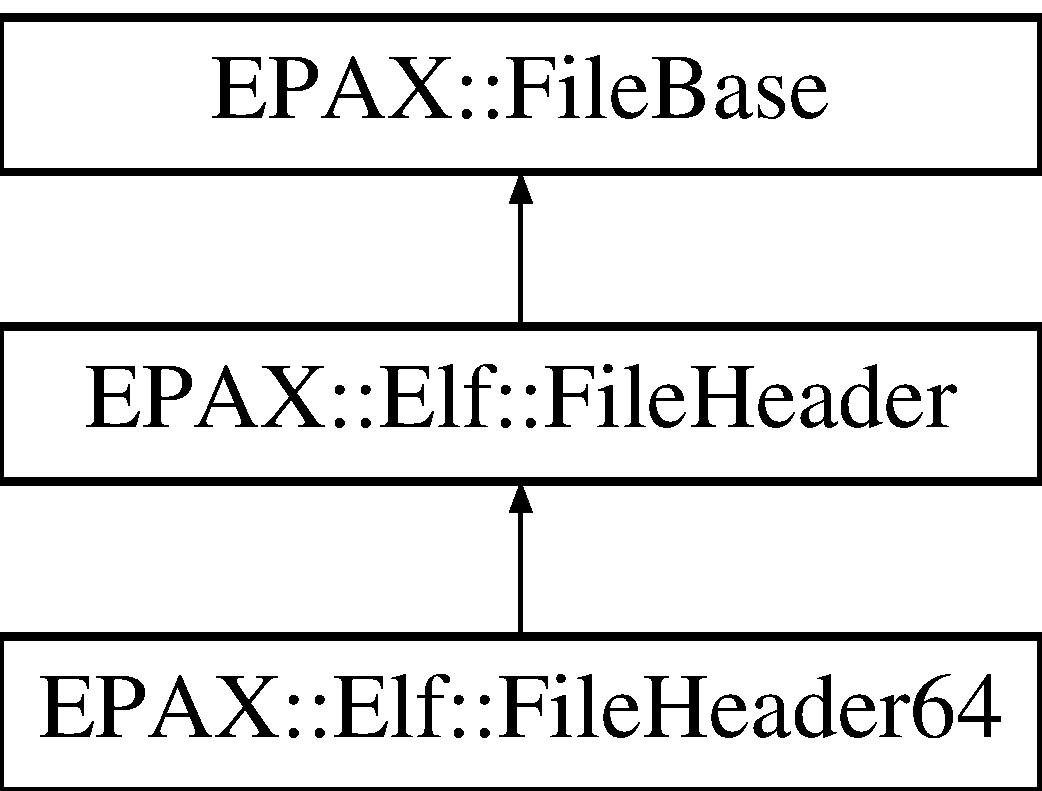
\includegraphics[height=3.000000cm]{class_e_p_a_x_1_1_elf_1_1_file_header64}
\end{center}
\end{figure}
\subsection*{\-Public \-Member \-Functions}
\begin{DoxyCompactItemize}
\item 
\hyperlink{class_e_p_a_x_1_1_elf_1_1_file_header64_a00cf5857d7fb0d99a29da523667b3561}{\-File\-Header64} (\hyperlink{class_e_p_a_x_1_1_base_binary}{\-Base\-Binary} $\ast$b, uint64\-\_\-t o)
\item 
virtual \hyperlink{class_e_p_a_x_1_1_elf_1_1_file_header64_a66a65eb185ba951c8529fdbd42919a66}{$\sim$\-File\-Header64} ()
\item 
uint64\-\_\-t \hyperlink{class_e_p_a_x_1_1_elf_1_1_file_header64_a0d5fb6bb80415565bec58de93526a2ea}{get\-Start\-Addr} ()
\item 
bool \hyperlink{class_e_p_a_x_1_1_elf_1_1_file_header64_a6a94d18eaee683c6bbe05f3b57f08efc}{verify} ()
\item 
bool \hyperlink{class_e_p_a_x_1_1_elf_1_1_file_header64_a6d992697b0003b0c63f9e9b6271de94a}{is\-A\-R\-M} ()
\item 
void \hyperlink{class_e_p_a_x_1_1_elf_1_1_file_header64_a121602d4ffb4f401b59cdb63303fc6c4}{describe} ()
\item 
uint32\-\_\-t \hyperlink{class_e_p_a_x_1_1_elf_1_1_file_header64_a525b2d31bb8ad212c197172006cd8b90}{get\-Section\-Count} ()
\item 
uint64\-\_\-t \hyperlink{class_e_p_a_x_1_1_elf_1_1_file_header64_ab4bf35526aa8997cdacbe51f401e15a2}{get\-Sec\-Table\-Offset} ()
\item 
uint32\-\_\-t \hyperlink{class_e_p_a_x_1_1_elf_1_1_file_header64_ad4c76f6ef875eccd6e453c61736d7e40}{get\-Shdr\-Size} ()
\item 
uint32\-\_\-t \hyperlink{class_e_p_a_x_1_1_elf_1_1_file_header64_a1e776b6ef8858287951a39a15626a6da}{get\-Shdr\-String\-Index} ()
\item 
uint32\-\_\-t \hyperlink{class_e_p_a_x_1_1_elf_1_1_file_header64_af0e3dc9b8ae0832bd9a24d2c72e09011}{get\-Segment\-Count} ()
\item 
uint64\-\_\-t \hyperlink{class_e_p_a_x_1_1_elf_1_1_file_header64_ad05c5e3abb06032413b058f5db1f3f9c}{get\-Seg\-Table\-Offset} ()
\item 
uint32\-\_\-t \hyperlink{class_e_p_a_x_1_1_elf_1_1_file_header64_a389cfa8997b78c7da91bfd980ad61a94}{get\-Phdr\-Size} ()
\item 
uint32\-\_\-t \hyperlink{class_e_p_a_x_1_1_elf_1_1_file_header64_a84696d5ac94bd884141c4306025b8ba4}{get\-File\-Type} ()
\end{DoxyCompactItemize}


\subsection{\-Detailed \-Description}


\-Definition at line 149 of file \-Elf\-Binary.\-hpp.



\subsection{\-Constructor \& \-Destructor \-Documentation}
\hypertarget{class_e_p_a_x_1_1_elf_1_1_file_header64_a00cf5857d7fb0d99a29da523667b3561}{\index{\-E\-P\-A\-X\-::\-Elf\-::\-File\-Header64@{\-E\-P\-A\-X\-::\-Elf\-::\-File\-Header64}!\-File\-Header64@{\-File\-Header64}}
\index{\-File\-Header64@{\-File\-Header64}!EPAX::Elf::FileHeader64@{\-E\-P\-A\-X\-::\-Elf\-::\-File\-Header64}}
\subsubsection[{\-File\-Header64}]{\setlength{\rightskip}{0pt plus 5cm}{\bf \-E\-P\-A\-X\-::\-Elf\-::\-File\-Header64\-::\-File\-Header64} (
\begin{DoxyParamCaption}
\item[{{\bf \-Base\-Binary} $\ast$}]{b, }
\item[{uint64\-\_\-t}]{o}
\end{DoxyParamCaption}
)}}\label{class_e_p_a_x_1_1_elf_1_1_file_header64_a00cf5857d7fb0d99a29da523667b3561}


\-Definition at line 404 of file \-Elf\-Binary.\-cpp.

\hypertarget{class_e_p_a_x_1_1_elf_1_1_file_header64_a66a65eb185ba951c8529fdbd42919a66}{\index{\-E\-P\-A\-X\-::\-Elf\-::\-File\-Header64@{\-E\-P\-A\-X\-::\-Elf\-::\-File\-Header64}!$\sim$\-File\-Header64@{$\sim$\-File\-Header64}}
\index{$\sim$\-File\-Header64@{$\sim$\-File\-Header64}!EPAX::Elf::FileHeader64@{\-E\-P\-A\-X\-::\-Elf\-::\-File\-Header64}}
\subsubsection[{$\sim$\-File\-Header64}]{\setlength{\rightskip}{0pt plus 5cm}virtual {\bf \-E\-P\-A\-X\-::\-Elf\-::\-File\-Header64\-::$\sim$\-File\-Header64} (
\begin{DoxyParamCaption}
{}
\end{DoxyParamCaption}
)\hspace{0.3cm}{\ttfamily  \mbox{[}inline, virtual\mbox{]}}}}\label{class_e_p_a_x_1_1_elf_1_1_file_header64_a66a65eb185ba951c8529fdbd42919a66}


\-Definition at line 152 of file \-Elf\-Binary.\-hpp.



\subsection{\-Member \-Function \-Documentation}
\hypertarget{class_e_p_a_x_1_1_elf_1_1_file_header64_a121602d4ffb4f401b59cdb63303fc6c4}{\index{\-E\-P\-A\-X\-::\-Elf\-::\-File\-Header64@{\-E\-P\-A\-X\-::\-Elf\-::\-File\-Header64}!describe@{describe}}
\index{describe@{describe}!EPAX::Elf::FileHeader64@{\-E\-P\-A\-X\-::\-Elf\-::\-File\-Header64}}
\subsubsection[{describe}]{\setlength{\rightskip}{0pt plus 5cm}void {\bf \-E\-P\-A\-X\-::\-Elf\-::\-File\-Header64\-::describe} (
\begin{DoxyParamCaption}
{}
\end{DoxyParamCaption}
)\hspace{0.3cm}{\ttfamily  \mbox{[}virtual\mbox{]}}}}\label{class_e_p_a_x_1_1_elf_1_1_file_header64_a121602d4ffb4f401b59cdb63303fc6c4}


\-Implements \hyperlink{class_e_p_a_x_1_1_elf_1_1_file_header_aeb0eeb9a943fe3382edc7e6b10c3d0d5}{\-E\-P\-A\-X\-::\-Elf\-::\-File\-Header}.



\-Definition at line 490 of file \-Elf\-Binary.\-cpp.

\hypertarget{class_e_p_a_x_1_1_elf_1_1_file_header64_a84696d5ac94bd884141c4306025b8ba4}{\index{\-E\-P\-A\-X\-::\-Elf\-::\-File\-Header64@{\-E\-P\-A\-X\-::\-Elf\-::\-File\-Header64}!get\-File\-Type@{get\-File\-Type}}
\index{get\-File\-Type@{get\-File\-Type}!EPAX::Elf::FileHeader64@{\-E\-P\-A\-X\-::\-Elf\-::\-File\-Header64}}
\subsubsection[{get\-File\-Type}]{\setlength{\rightskip}{0pt plus 5cm}uint32\-\_\-t {\bf \-E\-P\-A\-X\-::\-Elf\-::\-File\-Header64\-::get\-File\-Type} (
\begin{DoxyParamCaption}
{}
\end{DoxyParamCaption}
)\hspace{0.3cm}{\ttfamily  \mbox{[}virtual\mbox{]}}}}\label{class_e_p_a_x_1_1_elf_1_1_file_header64_a84696d5ac94bd884141c4306025b8ba4}


\-Implements \hyperlink{class_e_p_a_x_1_1_elf_1_1_file_header_ae36441d44c2fba9f42709566823b7d08}{\-E\-P\-A\-X\-::\-Elf\-::\-File\-Header}.



\-Definition at line 393 of file \-Elf\-Binary.\-cpp.

\hypertarget{class_e_p_a_x_1_1_elf_1_1_file_header64_a389cfa8997b78c7da91bfd980ad61a94}{\index{\-E\-P\-A\-X\-::\-Elf\-::\-File\-Header64@{\-E\-P\-A\-X\-::\-Elf\-::\-File\-Header64}!get\-Phdr\-Size@{get\-Phdr\-Size}}
\index{get\-Phdr\-Size@{get\-Phdr\-Size}!EPAX::Elf::FileHeader64@{\-E\-P\-A\-X\-::\-Elf\-::\-File\-Header64}}
\subsubsection[{get\-Phdr\-Size}]{\setlength{\rightskip}{0pt plus 5cm}uint32\-\_\-t {\bf \-E\-P\-A\-X\-::\-Elf\-::\-File\-Header64\-::get\-Phdr\-Size} (
\begin{DoxyParamCaption}
{}
\end{DoxyParamCaption}
)\hspace{0.3cm}{\ttfamily  \mbox{[}virtual\mbox{]}}}}\label{class_e_p_a_x_1_1_elf_1_1_file_header64_a389cfa8997b78c7da91bfd980ad61a94}


\-Implements \hyperlink{class_e_p_a_x_1_1_elf_1_1_file_header_a6d180c7702995629f962abd1cce29e2d}{\-E\-P\-A\-X\-::\-Elf\-::\-File\-Header}.



\-Definition at line 361 of file \-Elf\-Binary.\-cpp.

\hypertarget{class_e_p_a_x_1_1_elf_1_1_file_header64_ab4bf35526aa8997cdacbe51f401e15a2}{\index{\-E\-P\-A\-X\-::\-Elf\-::\-File\-Header64@{\-E\-P\-A\-X\-::\-Elf\-::\-File\-Header64}!get\-Sec\-Table\-Offset@{get\-Sec\-Table\-Offset}}
\index{get\-Sec\-Table\-Offset@{get\-Sec\-Table\-Offset}!EPAX::Elf::FileHeader64@{\-E\-P\-A\-X\-::\-Elf\-::\-File\-Header64}}
\subsubsection[{get\-Sec\-Table\-Offset}]{\setlength{\rightskip}{0pt plus 5cm}uint64\-\_\-t {\bf \-E\-P\-A\-X\-::\-Elf\-::\-File\-Header64\-::get\-Sec\-Table\-Offset} (
\begin{DoxyParamCaption}
{}
\end{DoxyParamCaption}
)\hspace{0.3cm}{\ttfamily  \mbox{[}virtual\mbox{]}}}}\label{class_e_p_a_x_1_1_elf_1_1_file_header64_ab4bf35526aa8997cdacbe51f401e15a2}


\-Implements \hyperlink{class_e_p_a_x_1_1_elf_1_1_file_header_a465040eb608f51272cb889e4fd0c61f1}{\-E\-P\-A\-X\-::\-Elf\-::\-File\-Header}.



\-Definition at line 337 of file \-Elf\-Binary.\-cpp.

\hypertarget{class_e_p_a_x_1_1_elf_1_1_file_header64_a525b2d31bb8ad212c197172006cd8b90}{\index{\-E\-P\-A\-X\-::\-Elf\-::\-File\-Header64@{\-E\-P\-A\-X\-::\-Elf\-::\-File\-Header64}!get\-Section\-Count@{get\-Section\-Count}}
\index{get\-Section\-Count@{get\-Section\-Count}!EPAX::Elf::FileHeader64@{\-E\-P\-A\-X\-::\-Elf\-::\-File\-Header64}}
\subsubsection[{get\-Section\-Count}]{\setlength{\rightskip}{0pt plus 5cm}uint32\-\_\-t {\bf \-E\-P\-A\-X\-::\-Elf\-::\-File\-Header64\-::get\-Section\-Count} (
\begin{DoxyParamCaption}
{}
\end{DoxyParamCaption}
)\hspace{0.3cm}{\ttfamily  \mbox{[}virtual\mbox{]}}}}\label{class_e_p_a_x_1_1_elf_1_1_file_header64_a525b2d31bb8ad212c197172006cd8b90}


\-Implements \hyperlink{class_e_p_a_x_1_1_elf_1_1_file_header_a80f2c4f1a3a4caee7bf6b9b6b7d20d92}{\-E\-P\-A\-X\-::\-Elf\-::\-File\-Header}.



\-Definition at line 377 of file \-Elf\-Binary.\-cpp.

\hypertarget{class_e_p_a_x_1_1_elf_1_1_file_header64_af0e3dc9b8ae0832bd9a24d2c72e09011}{\index{\-E\-P\-A\-X\-::\-Elf\-::\-File\-Header64@{\-E\-P\-A\-X\-::\-Elf\-::\-File\-Header64}!get\-Segment\-Count@{get\-Segment\-Count}}
\index{get\-Segment\-Count@{get\-Segment\-Count}!EPAX::Elf::FileHeader64@{\-E\-P\-A\-X\-::\-Elf\-::\-File\-Header64}}
\subsubsection[{get\-Segment\-Count}]{\setlength{\rightskip}{0pt plus 5cm}uint32\-\_\-t {\bf \-E\-P\-A\-X\-::\-Elf\-::\-File\-Header64\-::get\-Segment\-Count} (
\begin{DoxyParamCaption}
{}
\end{DoxyParamCaption}
)\hspace{0.3cm}{\ttfamily  \mbox{[}virtual\mbox{]}}}}\label{class_e_p_a_x_1_1_elf_1_1_file_header64_af0e3dc9b8ae0832bd9a24d2c72e09011}


\-Implements \hyperlink{class_e_p_a_x_1_1_elf_1_1_file_header_a016aee53224e8350e3b8452b1525aad5}{\-E\-P\-A\-X\-::\-Elf\-::\-File\-Header}.



\-Definition at line 385 of file \-Elf\-Binary.\-cpp.

\hypertarget{class_e_p_a_x_1_1_elf_1_1_file_header64_ad05c5e3abb06032413b058f5db1f3f9c}{\index{\-E\-P\-A\-X\-::\-Elf\-::\-File\-Header64@{\-E\-P\-A\-X\-::\-Elf\-::\-File\-Header64}!get\-Seg\-Table\-Offset@{get\-Seg\-Table\-Offset}}
\index{get\-Seg\-Table\-Offset@{get\-Seg\-Table\-Offset}!EPAX::Elf::FileHeader64@{\-E\-P\-A\-X\-::\-Elf\-::\-File\-Header64}}
\subsubsection[{get\-Seg\-Table\-Offset}]{\setlength{\rightskip}{0pt plus 5cm}uint64\-\_\-t {\bf \-E\-P\-A\-X\-::\-Elf\-::\-File\-Header64\-::get\-Seg\-Table\-Offset} (
\begin{DoxyParamCaption}
{}
\end{DoxyParamCaption}
)\hspace{0.3cm}{\ttfamily  \mbox{[}virtual\mbox{]}}}}\label{class_e_p_a_x_1_1_elf_1_1_file_header64_ad05c5e3abb06032413b058f5db1f3f9c}


\-Implements \hyperlink{class_e_p_a_x_1_1_elf_1_1_file_header_a428d1229cb7324696436d62b8c099239}{\-E\-P\-A\-X\-::\-Elf\-::\-File\-Header}.



\-Definition at line 353 of file \-Elf\-Binary.\-cpp.

\hypertarget{class_e_p_a_x_1_1_elf_1_1_file_header64_ad4c76f6ef875eccd6e453c61736d7e40}{\index{\-E\-P\-A\-X\-::\-Elf\-::\-File\-Header64@{\-E\-P\-A\-X\-::\-Elf\-::\-File\-Header64}!get\-Shdr\-Size@{get\-Shdr\-Size}}
\index{get\-Shdr\-Size@{get\-Shdr\-Size}!EPAX::Elf::FileHeader64@{\-E\-P\-A\-X\-::\-Elf\-::\-File\-Header64}}
\subsubsection[{get\-Shdr\-Size}]{\setlength{\rightskip}{0pt plus 5cm}uint32\-\_\-t {\bf \-E\-P\-A\-X\-::\-Elf\-::\-File\-Header64\-::get\-Shdr\-Size} (
\begin{DoxyParamCaption}
{}
\end{DoxyParamCaption}
)\hspace{0.3cm}{\ttfamily  \mbox{[}virtual\mbox{]}}}}\label{class_e_p_a_x_1_1_elf_1_1_file_header64_ad4c76f6ef875eccd6e453c61736d7e40}


\-Implements \hyperlink{class_e_p_a_x_1_1_elf_1_1_file_header_a52a8d42476216d7946039581f570958f}{\-E\-P\-A\-X\-::\-Elf\-::\-File\-Header}.



\-Definition at line 345 of file \-Elf\-Binary.\-cpp.

\hypertarget{class_e_p_a_x_1_1_elf_1_1_file_header64_a1e776b6ef8858287951a39a15626a6da}{\index{\-E\-P\-A\-X\-::\-Elf\-::\-File\-Header64@{\-E\-P\-A\-X\-::\-Elf\-::\-File\-Header64}!get\-Shdr\-String\-Index@{get\-Shdr\-String\-Index}}
\index{get\-Shdr\-String\-Index@{get\-Shdr\-String\-Index}!EPAX::Elf::FileHeader64@{\-E\-P\-A\-X\-::\-Elf\-::\-File\-Header64}}
\subsubsection[{get\-Shdr\-String\-Index}]{\setlength{\rightskip}{0pt plus 5cm}uint32\-\_\-t {\bf \-E\-P\-A\-X\-::\-Elf\-::\-File\-Header64\-::get\-Shdr\-String\-Index} (
\begin{DoxyParamCaption}
{}
\end{DoxyParamCaption}
)\hspace{0.3cm}{\ttfamily  \mbox{[}virtual\mbox{]}}}}\label{class_e_p_a_x_1_1_elf_1_1_file_header64_a1e776b6ef8858287951a39a15626a6da}


\-Implements \hyperlink{class_e_p_a_x_1_1_elf_1_1_file_header_aa1d63391748e17afd6ee45c9124d3cc1}{\-E\-P\-A\-X\-::\-Elf\-::\-File\-Header}.



\-Definition at line 369 of file \-Elf\-Binary.\-cpp.

\hypertarget{class_e_p_a_x_1_1_elf_1_1_file_header64_a0d5fb6bb80415565bec58de93526a2ea}{\index{\-E\-P\-A\-X\-::\-Elf\-::\-File\-Header64@{\-E\-P\-A\-X\-::\-Elf\-::\-File\-Header64}!get\-Start\-Addr@{get\-Start\-Addr}}
\index{get\-Start\-Addr@{get\-Start\-Addr}!EPAX::Elf::FileHeader64@{\-E\-P\-A\-X\-::\-Elf\-::\-File\-Header64}}
\subsubsection[{get\-Start\-Addr}]{\setlength{\rightskip}{0pt plus 5cm}uint64\-\_\-t {\bf \-E\-P\-A\-X\-::\-Elf\-::\-File\-Header64\-::get\-Start\-Addr} (
\begin{DoxyParamCaption}
{}
\end{DoxyParamCaption}
)\hspace{0.3cm}{\ttfamily  \mbox{[}virtual\mbox{]}}}}\label{class_e_p_a_x_1_1_elf_1_1_file_header64_a0d5fb6bb80415565bec58de93526a2ea}


\-Implements \hyperlink{class_e_p_a_x_1_1_elf_1_1_file_header_abdf6ca1b4c9bb4e4467ad7467c44730e}{\-E\-P\-A\-X\-::\-Elf\-::\-File\-Header}.



\-Definition at line 415 of file \-Elf\-Binary.\-cpp.

\hypertarget{class_e_p_a_x_1_1_elf_1_1_file_header64_a6d992697b0003b0c63f9e9b6271de94a}{\index{\-E\-P\-A\-X\-::\-Elf\-::\-File\-Header64@{\-E\-P\-A\-X\-::\-Elf\-::\-File\-Header64}!is\-A\-R\-M@{is\-A\-R\-M}}
\index{is\-A\-R\-M@{is\-A\-R\-M}!EPAX::Elf::FileHeader64@{\-E\-P\-A\-X\-::\-Elf\-::\-File\-Header64}}
\subsubsection[{is\-A\-R\-M}]{\setlength{\rightskip}{0pt plus 5cm}bool {\bf \-E\-P\-A\-X\-::\-Elf\-::\-File\-Header64\-::is\-A\-R\-M} (
\begin{DoxyParamCaption}
{}
\end{DoxyParamCaption}
)\hspace{0.3cm}{\ttfamily  \mbox{[}virtual\mbox{]}}}}\label{class_e_p_a_x_1_1_elf_1_1_file_header64_a6d992697b0003b0c63f9e9b6271de94a}


\-Implements \hyperlink{class_e_p_a_x_1_1_elf_1_1_file_header_a7213d758b36fccdb80c7c3068155cdee}{\-E\-P\-A\-X\-::\-Elf\-::\-File\-Header}.



\-Definition at line 453 of file \-Elf\-Binary.\-cpp.

\hypertarget{class_e_p_a_x_1_1_elf_1_1_file_header64_a6a94d18eaee683c6bbe05f3b57f08efc}{\index{\-E\-P\-A\-X\-::\-Elf\-::\-File\-Header64@{\-E\-P\-A\-X\-::\-Elf\-::\-File\-Header64}!verify@{verify}}
\index{verify@{verify}!EPAX::Elf::FileHeader64@{\-E\-P\-A\-X\-::\-Elf\-::\-File\-Header64}}
\subsubsection[{verify}]{\setlength{\rightskip}{0pt plus 5cm}bool {\bf \-E\-P\-A\-X\-::\-Elf\-::\-File\-Header64\-::verify} (
\begin{DoxyParamCaption}
{}
\end{DoxyParamCaption}
)\hspace{0.3cm}{\ttfamily  \mbox{[}virtual\mbox{]}}}}\label{class_e_p_a_x_1_1_elf_1_1_file_header64_a6a94d18eaee683c6bbe05f3b57f08efc}


\-Implements \hyperlink{class_e_p_a_x_1_1_elf_1_1_file_header_a3ca4cd831fa0b4406c0d4864b659c91c}{\-E\-P\-A\-X\-::\-Elf\-::\-File\-Header}.



\-Definition at line 433 of file \-Elf\-Binary.\-cpp.



\-The documentation for this class was generated from the following files\-:\begin{DoxyCompactItemize}
\item 
\hyperlink{_elf_binary_8hpp}{\-Elf\-Binary.\-hpp}\item 
\hyperlink{_elf_binary_8cpp}{\-Elf\-Binary.\-cpp}\end{DoxyCompactItemize}

\hypertarget{class_e_p_a_x_1_1_function}{\section{\-E\-P\-A\-X\-:\-:\-Function \-Class \-Reference}
\label{class_e_p_a_x_1_1_function}\index{\-E\-P\-A\-X\-::\-Function@{\-E\-P\-A\-X\-::\-Function}}
}


{\ttfamily \#include $<$\-Function.\-hpp$>$}

\-Inheritance diagram for \-E\-P\-A\-X\-:\-:\-Function\-:\begin{figure}[H]
\begin{center}
\leavevmode
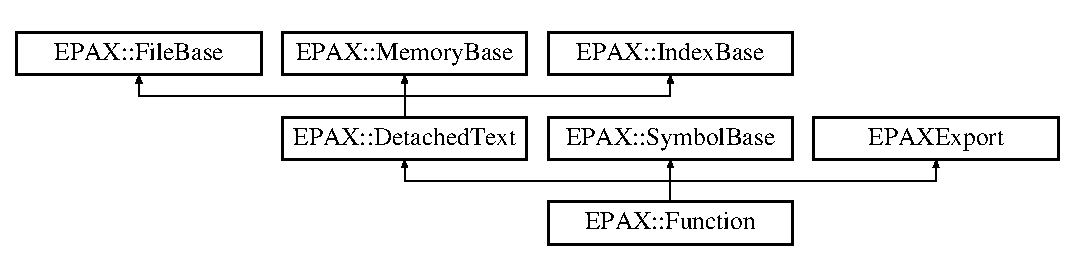
\includegraphics[height=3.000000cm]{class_e_p_a_x_1_1_function}
\end{center}
\end{figure}
\subsection*{\-Public \-Member \-Functions}
\begin{DoxyCompactItemize}
\item 
\hyperlink{class_e_p_a_x_1_1_function_ac873403538ebdbf41e3dd50e6717ed8e}{\-Function} (\hyperlink{class_e_p_a_x_1_1_base_binary}{\-Base\-Binary} $\ast$b, uint64\-\_\-t o, uint64\-\_\-t s, uint64\-\_\-t a, uint32\-\_\-t i, \hyperlink{class_e_p_a_x_1_1_symbol}{\-Symbol} $\ast$y)
\item 
virtual \hyperlink{class_e_p_a_x_1_1_function_ab25462d1e27b1619c989c82d8f052b5e}{$\sim$\-Function} ()
\item 
void \hyperlink{class_e_p_a_x_1_1_function_a82cd9c2c9b4210f2c189e60f13445b77}{print} (std\-::ostream \&stream=std\-::cout)
\item 
\hyperlink{class_e_p_a_x_1_1_control_flow}{\-Control\-Flow} $\ast$ \hyperlink{class_e_p_a_x_1_1_function_a21ef5f83eff1f260deea42edd3f9288a}{get\-Control\-Flow} ()
\item 
uint32\-\_\-t \hyperlink{class_e_p_a_x_1_1_function_ab6ab497ee5a9fd8794a6fc007c28322e}{count\-Basic\-Blocks} ()
\item 
\hyperlink{class_e_p_a_x_1_1_basic_block}{\-Basic\-Block} $\ast$ \hyperlink{class_e_p_a_x_1_1_function_affd34e44b8b26be10b2eaeafa90c72e2}{find\-Basic\-Block} (uint64\-\_\-t addr)
\item 
\hyperlink{class_e_p_a_x_1_1_basic_block}{\-Basic\-Block} $\ast$ \hyperlink{class_e_p_a_x_1_1_function_aab41091efc192b4da0912746b4b03c4c}{get\-Basic\-Block} (uint32\-\_\-t idx)
\item 
uint32\-\_\-t \hyperlink{class_e_p_a_x_1_1_function_aa7cf28ca6fd8dda7391a142a3fce6f20}{count\-Instructions} ()
\item 
\hyperlink{class_e_p_a_x_1_1_instruction}{\-Instruction} $\ast$ \hyperlink{class_e_p_a_x_1_1_function_a0d6c6cd2a010690550065de7865591d7}{find\-Instruction} (uint64\-\_\-t addr)
\item 
\hyperlink{class_e_p_a_x_1_1_instruction}{\-Instruction} $\ast$ \hyperlink{class_e_p_a_x_1_1_function_a80400b0ca8d9047bff8dd588d8a03918}{get\-Instruction} (uint32\-\_\-t idx)
\item 
void \hyperlink{class_e_p_a_x_1_1_function_a0388e0d1e3953da9e259711c4352c146}{disassemble} ()
\end{DoxyCompactItemize}
\subsection*{\-Static \-Public \-Member \-Functions}
\begin{DoxyCompactItemize}
\item 
static void \hyperlink{class_e_p_a_x_1_1_function_acf8e6e84f93e87bab13edc2c03929425}{print\-Header} (std\-::ostream \&stream=std\-::cout)
\end{DoxyCompactItemize}


\subsection{\-Detailed \-Description}


\-Definition at line 55 of file \-Function.\-hpp.



\subsection{\-Constructor \& \-Destructor \-Documentation}
\hypertarget{class_e_p_a_x_1_1_function_ac873403538ebdbf41e3dd50e6717ed8e}{\index{\-E\-P\-A\-X\-::\-Function@{\-E\-P\-A\-X\-::\-Function}!\-Function@{\-Function}}
\index{\-Function@{\-Function}!EPAX::Function@{\-E\-P\-A\-X\-::\-Function}}
\subsubsection[{\-Function}]{\setlength{\rightskip}{0pt plus 5cm}{\bf \-E\-P\-A\-X\-::\-Function\-::\-Function} (
\begin{DoxyParamCaption}
\item[{{\bf \-Base\-Binary} $\ast$}]{b, }
\item[{uint64\-\_\-t}]{o, }
\item[{uint64\-\_\-t}]{s, }
\item[{uint64\-\_\-t}]{a, }
\item[{uint32\-\_\-t}]{i, }
\item[{{\bf \-Symbol} $\ast$}]{y}
\end{DoxyParamCaption}
)}}\label{class_e_p_a_x_1_1_function_ac873403538ebdbf41e3dd50e6717ed8e}


\-Definition at line 154 of file \-Function.\-cpp.

\hypertarget{class_e_p_a_x_1_1_function_ab25462d1e27b1619c989c82d8f052b5e}{\index{\-E\-P\-A\-X\-::\-Function@{\-E\-P\-A\-X\-::\-Function}!$\sim$\-Function@{$\sim$\-Function}}
\index{$\sim$\-Function@{$\sim$\-Function}!EPAX::Function@{\-E\-P\-A\-X\-::\-Function}}
\subsubsection[{$\sim$\-Function}]{\setlength{\rightskip}{0pt plus 5cm}{\bf \-E\-P\-A\-X\-::\-Function\-::$\sim$\-Function} (
\begin{DoxyParamCaption}
{}
\end{DoxyParamCaption}
)\hspace{0.3cm}{\ttfamily  \mbox{[}virtual\mbox{]}}}}\label{class_e_p_a_x_1_1_function_ab25462d1e27b1619c989c82d8f052b5e}


\-Definition at line 166 of file \-Function.\-cpp.



\subsection{\-Member \-Function \-Documentation}
\hypertarget{class_e_p_a_x_1_1_function_ab6ab497ee5a9fd8794a6fc007c28322e}{\index{\-E\-P\-A\-X\-::\-Function@{\-E\-P\-A\-X\-::\-Function}!count\-Basic\-Blocks@{count\-Basic\-Blocks}}
\index{count\-Basic\-Blocks@{count\-Basic\-Blocks}!EPAX::Function@{\-E\-P\-A\-X\-::\-Function}}
\subsubsection[{count\-Basic\-Blocks}]{\setlength{\rightskip}{0pt plus 5cm}uint32\-\_\-t {\bf \-E\-P\-A\-X\-::\-Function\-::count\-Basic\-Blocks} (
\begin{DoxyParamCaption}
{}
\end{DoxyParamCaption}
)}}\label{class_e_p_a_x_1_1_function_ab6ab497ee5a9fd8794a6fc007c28322e}


\-Definition at line 198 of file \-Function.\-cpp.

\hypertarget{class_e_p_a_x_1_1_function_aa7cf28ca6fd8dda7391a142a3fce6f20}{\index{\-E\-P\-A\-X\-::\-Function@{\-E\-P\-A\-X\-::\-Function}!count\-Instructions@{count\-Instructions}}
\index{count\-Instructions@{count\-Instructions}!EPAX::Function@{\-E\-P\-A\-X\-::\-Function}}
\subsubsection[{count\-Instructions}]{\setlength{\rightskip}{0pt plus 5cm}uint32\-\_\-t {\bf \-E\-P\-A\-X\-::\-Function\-::count\-Instructions} (
\begin{DoxyParamCaption}
{}
\end{DoxyParamCaption}
)}}\label{class_e_p_a_x_1_1_function_aa7cf28ca6fd8dda7391a142a3fce6f20}


\-Definition at line 220 of file \-Function.\-cpp.

\hypertarget{class_e_p_a_x_1_1_function_a0388e0d1e3953da9e259711c4352c146}{\index{\-E\-P\-A\-X\-::\-Function@{\-E\-P\-A\-X\-::\-Function}!disassemble@{disassemble}}
\index{disassemble@{disassemble}!EPAX::Function@{\-E\-P\-A\-X\-::\-Function}}
\subsubsection[{disassemble}]{\setlength{\rightskip}{0pt plus 5cm}void {\bf \-E\-P\-A\-X\-::\-Function\-::disassemble} (
\begin{DoxyParamCaption}
{}
\end{DoxyParamCaption}
)}}\label{class_e_p_a_x_1_1_function_a0388e0d1e3953da9e259711c4352c146}


\-Definition at line 172 of file \-Function.\-cpp.

\hypertarget{class_e_p_a_x_1_1_function_affd34e44b8b26be10b2eaeafa90c72e2}{\index{\-E\-P\-A\-X\-::\-Function@{\-E\-P\-A\-X\-::\-Function}!find\-Basic\-Block@{find\-Basic\-Block}}
\index{find\-Basic\-Block@{find\-Basic\-Block}!EPAX::Function@{\-E\-P\-A\-X\-::\-Function}}
\subsubsection[{find\-Basic\-Block}]{\setlength{\rightskip}{0pt plus 5cm}{\bf \-Basic\-Block} $\ast$ {\bf \-E\-P\-A\-X\-::\-Function\-::find\-Basic\-Block} (
\begin{DoxyParamCaption}
\item[{uint64\-\_\-t}]{addr}
\end{DoxyParamCaption}
)}}\label{class_e_p_a_x_1_1_function_affd34e44b8b26be10b2eaeafa90c72e2}


\-Definition at line 205 of file \-Function.\-cpp.

\hypertarget{class_e_p_a_x_1_1_function_a0d6c6cd2a010690550065de7865591d7}{\index{\-E\-P\-A\-X\-::\-Function@{\-E\-P\-A\-X\-::\-Function}!find\-Instruction@{find\-Instruction}}
\index{find\-Instruction@{find\-Instruction}!EPAX::Function@{\-E\-P\-A\-X\-::\-Function}}
\subsubsection[{find\-Instruction}]{\setlength{\rightskip}{0pt plus 5cm}{\bf \-Instruction} $\ast$ {\bf \-E\-P\-A\-X\-::\-Function\-::find\-Instruction} (
\begin{DoxyParamCaption}
\item[{uint64\-\_\-t}]{addr}
\end{DoxyParamCaption}
)}}\label{class_e_p_a_x_1_1_function_a0d6c6cd2a010690550065de7865591d7}


\-Definition at line 227 of file \-Function.\-cpp.

\hypertarget{class_e_p_a_x_1_1_function_aab41091efc192b4da0912746b4b03c4c}{\index{\-E\-P\-A\-X\-::\-Function@{\-E\-P\-A\-X\-::\-Function}!get\-Basic\-Block@{get\-Basic\-Block}}
\index{get\-Basic\-Block@{get\-Basic\-Block}!EPAX::Function@{\-E\-P\-A\-X\-::\-Function}}
\subsubsection[{get\-Basic\-Block}]{\setlength{\rightskip}{0pt plus 5cm}{\bf \-Basic\-Block} $\ast$ {\bf \-E\-P\-A\-X\-::\-Function\-::get\-Basic\-Block} (
\begin{DoxyParamCaption}
\item[{uint32\-\_\-t}]{idx}
\end{DoxyParamCaption}
)}}\label{class_e_p_a_x_1_1_function_aab41091efc192b4da0912746b4b03c4c}


\-Definition at line 213 of file \-Function.\-cpp.

\hypertarget{class_e_p_a_x_1_1_function_a21ef5f83eff1f260deea42edd3f9288a}{\index{\-E\-P\-A\-X\-::\-Function@{\-E\-P\-A\-X\-::\-Function}!get\-Control\-Flow@{get\-Control\-Flow}}
\index{get\-Control\-Flow@{get\-Control\-Flow}!EPAX::Function@{\-E\-P\-A\-X\-::\-Function}}
\subsubsection[{get\-Control\-Flow}]{\setlength{\rightskip}{0pt plus 5cm}{\bf \-Control\-Flow}$\ast$ {\bf \-E\-P\-A\-X\-::\-Function\-::get\-Control\-Flow} (
\begin{DoxyParamCaption}
{}
\end{DoxyParamCaption}
)\hspace{0.3cm}{\ttfamily  \mbox{[}inline\mbox{]}}}}\label{class_e_p_a_x_1_1_function_a21ef5f83eff1f260deea42edd3f9288a}


\-Definition at line 68 of file \-Function.\-hpp.

\hypertarget{class_e_p_a_x_1_1_function_a80400b0ca8d9047bff8dd588d8a03918}{\index{\-E\-P\-A\-X\-::\-Function@{\-E\-P\-A\-X\-::\-Function}!get\-Instruction@{get\-Instruction}}
\index{get\-Instruction@{get\-Instruction}!EPAX::Function@{\-E\-P\-A\-X\-::\-Function}}
\subsubsection[{get\-Instruction}]{\setlength{\rightskip}{0pt plus 5cm}{\bf \-Instruction} $\ast$ {\bf \-E\-P\-A\-X\-::\-Function\-::get\-Instruction} (
\begin{DoxyParamCaption}
\item[{uint32\-\_\-t}]{idx}
\end{DoxyParamCaption}
)}}\label{class_e_p_a_x_1_1_function_a80400b0ca8d9047bff8dd588d8a03918}


\-Definition at line 234 of file \-Function.\-cpp.

\hypertarget{class_e_p_a_x_1_1_function_a82cd9c2c9b4210f2c189e60f13445b77}{\index{\-E\-P\-A\-X\-::\-Function@{\-E\-P\-A\-X\-::\-Function}!print@{print}}
\index{print@{print}!EPAX::Function@{\-E\-P\-A\-X\-::\-Function}}
\subsubsection[{print}]{\setlength{\rightskip}{0pt plus 5cm}void {\bf \-E\-P\-A\-X\-::\-Function\-::print} (
\begin{DoxyParamCaption}
\item[{std\-::ostream \&}]{stream = {\ttfamily std\-:\-:cout}}
\end{DoxyParamCaption}
)\hspace{0.3cm}{\ttfamily  \mbox{[}virtual\mbox{]}}}}\label{class_e_p_a_x_1_1_function_a82cd9c2c9b4210f2c189e60f13445b77}


\-Reimplemented from \hyperlink{class_e_p_a_x_1_1_detached_text_a8a32ccd60ccd9a710a84301b4c483902}{\-E\-P\-A\-X\-::\-Detached\-Text}.



\-Definition at line 186 of file \-Function.\-cpp.

\hypertarget{class_e_p_a_x_1_1_function_acf8e6e84f93e87bab13edc2c03929425}{\index{\-E\-P\-A\-X\-::\-Function@{\-E\-P\-A\-X\-::\-Function}!print\-Header@{print\-Header}}
\index{print\-Header@{print\-Header}!EPAX::Function@{\-E\-P\-A\-X\-::\-Function}}
\subsubsection[{print\-Header}]{\setlength{\rightskip}{0pt plus 5cm}void {\bf \-E\-P\-A\-X\-::\-Function\-::print\-Header} (
\begin{DoxyParamCaption}
\item[{std\-::ostream \&}]{stream = {\ttfamily std\-:\-:cout}}
\end{DoxyParamCaption}
)\hspace{0.3cm}{\ttfamily  \mbox{[}static\mbox{]}}}}\label{class_e_p_a_x_1_1_function_acf8e6e84f93e87bab13edc2c03929425}


\-Definition at line 178 of file \-Function.\-cpp.



\-The documentation for this class was generated from the following files\-:\begin{DoxyCompactItemize}
\item 
\hyperlink{_function_8hpp}{\-Function.\-hpp}\item 
\hyperlink{_function_8cpp}{\-Function.\-cpp}\end{DoxyCompactItemize}

\hypertarget{class_e_p_a_x_1_1_index_base}{\section{\-E\-P\-A\-X\-:\-:\-Index\-Base \-Class \-Reference}
\label{class_e_p_a_x_1_1_index_base}\index{\-E\-P\-A\-X\-::\-Index\-Base@{\-E\-P\-A\-X\-::\-Index\-Base}}
}


{\ttfamily \#include $<$\-Base\-Class.\-hpp$>$}

\-Inheritance diagram for \-E\-P\-A\-X\-:\-:\-Index\-Base\-:\begin{figure}[H]
\begin{center}
\leavevmode
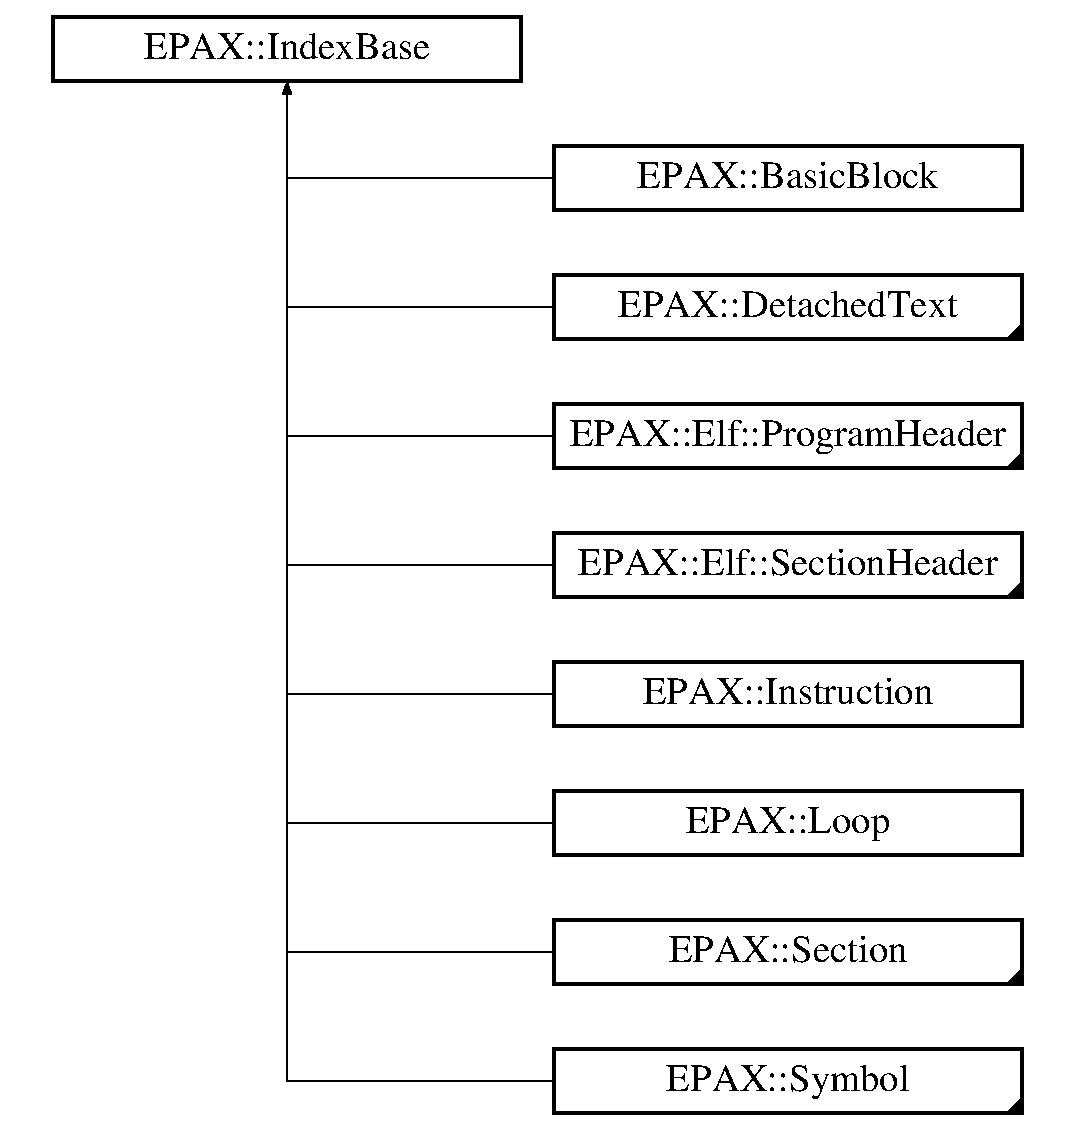
\includegraphics[height=9.000000cm]{class_e_p_a_x_1_1_index_base}
\end{center}
\end{figure}
\subsection*{\-Public \-Member \-Functions}
\begin{DoxyCompactItemize}
\item 
\hyperlink{class_e_p_a_x_1_1_index_base_a4b635a78fd95d44e733f41baf9c79220}{\-Index\-Base} (uint32\-\_\-t i)
\item 
virtual \hyperlink{class_e_p_a_x_1_1_index_base_aed5103698843436e247cfa6920c3677e}{$\sim$\-Index\-Base} ()
\item 
uint32\-\_\-t \hyperlink{class_e_p_a_x_1_1_index_base_a6115276ca197b32637ed030b7afdc58e}{get\-Index} ()
\item 
void \hyperlink{class_e_p_a_x_1_1_index_base_ae5b590c1e70d98d831c740b0eeca0cb8}{set\-Index} (uint32\-\_\-t i)
\end{DoxyCompactItemize}


\subsection{\-Detailed \-Description}


\-Definition at line 94 of file \-Base\-Class.\-hpp.



\subsection{\-Constructor \& \-Destructor \-Documentation}
\hypertarget{class_e_p_a_x_1_1_index_base_a4b635a78fd95d44e733f41baf9c79220}{\index{\-E\-P\-A\-X\-::\-Index\-Base@{\-E\-P\-A\-X\-::\-Index\-Base}!\-Index\-Base@{\-Index\-Base}}
\index{\-Index\-Base@{\-Index\-Base}!EPAX::IndexBase@{\-E\-P\-A\-X\-::\-Index\-Base}}
\subsubsection[{\-Index\-Base}]{\setlength{\rightskip}{0pt plus 5cm}{\bf \-E\-P\-A\-X\-::\-Index\-Base\-::\-Index\-Base} (
\begin{DoxyParamCaption}
\item[{uint32\-\_\-t}]{i}
\end{DoxyParamCaption}
)\hspace{0.3cm}{\ttfamily  \mbox{[}inline\mbox{]}}}}\label{class_e_p_a_x_1_1_index_base_a4b635a78fd95d44e733f41baf9c79220}


\-Definition at line 99 of file \-Base\-Class.\-hpp.

\hypertarget{class_e_p_a_x_1_1_index_base_aed5103698843436e247cfa6920c3677e}{\index{\-E\-P\-A\-X\-::\-Index\-Base@{\-E\-P\-A\-X\-::\-Index\-Base}!$\sim$\-Index\-Base@{$\sim$\-Index\-Base}}
\index{$\sim$\-Index\-Base@{$\sim$\-Index\-Base}!EPAX::IndexBase@{\-E\-P\-A\-X\-::\-Index\-Base}}
\subsubsection[{$\sim$\-Index\-Base}]{\setlength{\rightskip}{0pt plus 5cm}virtual {\bf \-E\-P\-A\-X\-::\-Index\-Base\-::$\sim$\-Index\-Base} (
\begin{DoxyParamCaption}
{}
\end{DoxyParamCaption}
)\hspace{0.3cm}{\ttfamily  \mbox{[}inline, virtual\mbox{]}}}}\label{class_e_p_a_x_1_1_index_base_aed5103698843436e247cfa6920c3677e}


\-Definition at line 101 of file \-Base\-Class.\-hpp.



\subsection{\-Member \-Function \-Documentation}
\hypertarget{class_e_p_a_x_1_1_index_base_a6115276ca197b32637ed030b7afdc58e}{\index{\-E\-P\-A\-X\-::\-Index\-Base@{\-E\-P\-A\-X\-::\-Index\-Base}!get\-Index@{get\-Index}}
\index{get\-Index@{get\-Index}!EPAX::IndexBase@{\-E\-P\-A\-X\-::\-Index\-Base}}
\subsubsection[{get\-Index}]{\setlength{\rightskip}{0pt plus 5cm}uint32\-\_\-t {\bf \-E\-P\-A\-X\-::\-Index\-Base\-::get\-Index} (
\begin{DoxyParamCaption}
{}
\end{DoxyParamCaption}
)\hspace{0.3cm}{\ttfamily  \mbox{[}inline\mbox{]}}}}\label{class_e_p_a_x_1_1_index_base_a6115276ca197b32637ed030b7afdc58e}


\-Definition at line 103 of file \-Base\-Class.\-hpp.

\hypertarget{class_e_p_a_x_1_1_index_base_ae5b590c1e70d98d831c740b0eeca0cb8}{\index{\-E\-P\-A\-X\-::\-Index\-Base@{\-E\-P\-A\-X\-::\-Index\-Base}!set\-Index@{set\-Index}}
\index{set\-Index@{set\-Index}!EPAX::IndexBase@{\-E\-P\-A\-X\-::\-Index\-Base}}
\subsubsection[{set\-Index}]{\setlength{\rightskip}{0pt plus 5cm}void {\bf \-E\-P\-A\-X\-::\-Index\-Base\-::set\-Index} (
\begin{DoxyParamCaption}
\item[{uint32\-\_\-t}]{i}
\end{DoxyParamCaption}
)\hspace{0.3cm}{\ttfamily  \mbox{[}inline\mbox{]}}}}\label{class_e_p_a_x_1_1_index_base_ae5b590c1e70d98d831c740b0eeca0cb8}


\-Definition at line 104 of file \-Base\-Class.\-hpp.



\-The documentation for this class was generated from the following file\-:\begin{DoxyCompactItemize}
\item 
\hyperlink{_base_class_8hpp}{\-Base\-Class.\-hpp}\end{DoxyCompactItemize}

\hypertarget{class_e_p_a_x_1_1_input_file}{\section{\-E\-P\-A\-X\-:\-:\-Input\-File \-Class \-Reference}
\label{class_e_p_a_x_1_1_input_file}\index{\-E\-P\-A\-X\-::\-Input\-File@{\-E\-P\-A\-X\-::\-Input\-File}}
}


{\ttfamily \#include $<$\-Input\-File.\-hpp$>$}

\-Inheritance diagram for \-E\-P\-A\-X\-:\-:\-Input\-File\-:\begin{figure}[H]
\begin{center}
\leavevmode
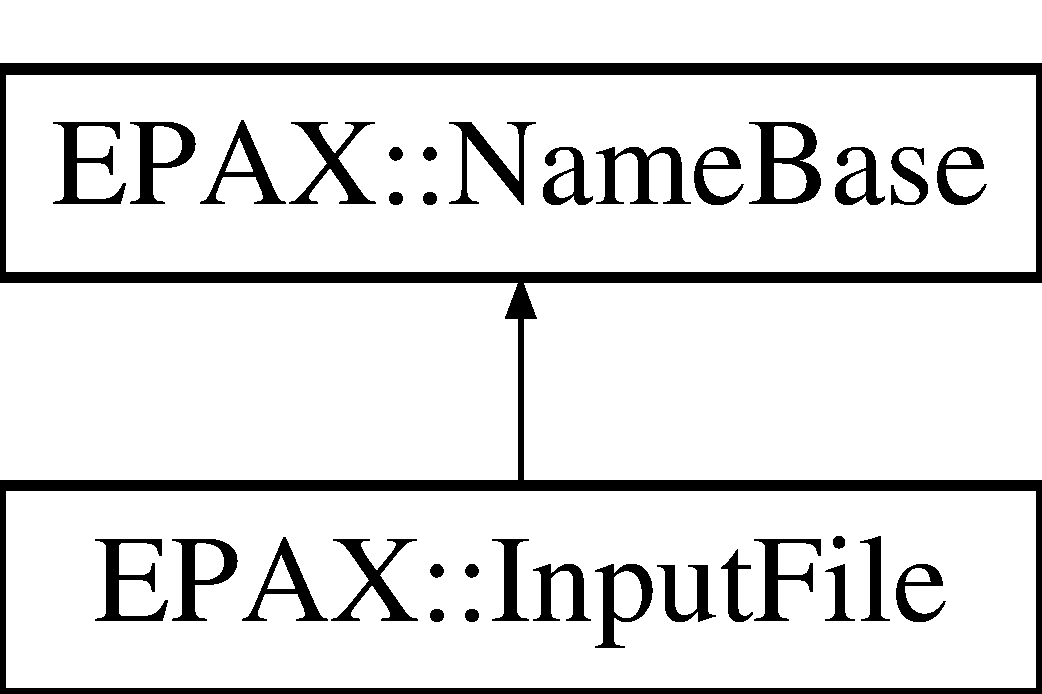
\includegraphics[height=2.000000cm]{class_e_p_a_x_1_1_input_file}
\end{center}
\end{figure}
\subsection*{\-Public \-Member \-Functions}
\begin{DoxyCompactItemize}
\item 
\hyperlink{class_e_p_a_x_1_1_input_file_a78bd5d3b22843d59b7a596fd714928ce}{\-Input\-File} (std\-::string n)
\item 
virtual \hyperlink{class_e_p_a_x_1_1_input_file_a89d4cd0f11e75985ae1d7528e864016f}{$\sim$\-Input\-File} ()
\item 
uint64\-\_\-t \hyperlink{class_e_p_a_x_1_1_input_file_a4b7b6d515479e8d3006041a34f15b526}{get\-Bytes} (uint64\-\_\-t offset, uint64\-\_\-t size, \hyperlink{_e_p_a_x_common_internal_8hpp_a17755bdd71c02e656c667b16de61dd7b}{rawbyte\-\_\-t} $\ast$buffer)
\item 
uint64\-\_\-t \hyperlink{class_e_p_a_x_1_1_input_file_aad97988077800254811c944ad6858d1f}{get\-File\-Size} ()
\end{DoxyCompactItemize}


\subsection{\-Detailed \-Description}


\-Definition at line 32 of file \-Input\-File.\-hpp.



\subsection{\-Constructor \& \-Destructor \-Documentation}
\hypertarget{class_e_p_a_x_1_1_input_file_a78bd5d3b22843d59b7a596fd714928ce}{\index{\-E\-P\-A\-X\-::\-Input\-File@{\-E\-P\-A\-X\-::\-Input\-File}!\-Input\-File@{\-Input\-File}}
\index{\-Input\-File@{\-Input\-File}!EPAX::InputFile@{\-E\-P\-A\-X\-::\-Input\-File}}
\subsubsection[{\-Input\-File}]{\setlength{\rightskip}{0pt plus 5cm}{\bf \-E\-P\-A\-X\-::\-Input\-File\-::\-Input\-File} (
\begin{DoxyParamCaption}
\item[{std\-::string}]{n}
\end{DoxyParamCaption}
)}}\label{class_e_p_a_x_1_1_input_file_a78bd5d3b22843d59b7a596fd714928ce}


\-Definition at line 30 of file \-Input\-File.\-cpp.

\hypertarget{class_e_p_a_x_1_1_input_file_a89d4cd0f11e75985ae1d7528e864016f}{\index{\-E\-P\-A\-X\-::\-Input\-File@{\-E\-P\-A\-X\-::\-Input\-File}!$\sim$\-Input\-File@{$\sim$\-Input\-File}}
\index{$\sim$\-Input\-File@{$\sim$\-Input\-File}!EPAX::InputFile@{\-E\-P\-A\-X\-::\-Input\-File}}
\subsubsection[{$\sim$\-Input\-File}]{\setlength{\rightskip}{0pt plus 5cm}{\bf \-E\-P\-A\-X\-::\-Input\-File\-::$\sim$\-Input\-File} (
\begin{DoxyParamCaption}
{}
\end{DoxyParamCaption}
)\hspace{0.3cm}{\ttfamily  \mbox{[}virtual\mbox{]}}}}\label{class_e_p_a_x_1_1_input_file_a89d4cd0f11e75985ae1d7528e864016f}


\-Definition at line 38 of file \-Input\-File.\-cpp.



\subsection{\-Member \-Function \-Documentation}
\hypertarget{class_e_p_a_x_1_1_input_file_a4b7b6d515479e8d3006041a34f15b526}{\index{\-E\-P\-A\-X\-::\-Input\-File@{\-E\-P\-A\-X\-::\-Input\-File}!get\-Bytes@{get\-Bytes}}
\index{get\-Bytes@{get\-Bytes}!EPAX::InputFile@{\-E\-P\-A\-X\-::\-Input\-File}}
\subsubsection[{get\-Bytes}]{\setlength{\rightskip}{0pt plus 5cm}uint64\-\_\-t {\bf \-E\-P\-A\-X\-::\-Input\-File\-::get\-Bytes} (
\begin{DoxyParamCaption}
\item[{uint64\-\_\-t}]{offset, }
\item[{uint64\-\_\-t}]{size, }
\item[{{\bf rawbyte\-\_\-t} $\ast$}]{buffer}
\end{DoxyParamCaption}
)}}\label{class_e_p_a_x_1_1_input_file_a4b7b6d515479e8d3006041a34f15b526}


\-Definition at line 54 of file \-Input\-File.\-cpp.

\hypertarget{class_e_p_a_x_1_1_input_file_aad97988077800254811c944ad6858d1f}{\index{\-E\-P\-A\-X\-::\-Input\-File@{\-E\-P\-A\-X\-::\-Input\-File}!get\-File\-Size@{get\-File\-Size}}
\index{get\-File\-Size@{get\-File\-Size}!EPAX::InputFile@{\-E\-P\-A\-X\-::\-Input\-File}}
\subsubsection[{get\-File\-Size}]{\setlength{\rightskip}{0pt plus 5cm}uint64\-\_\-t {\bf \-E\-P\-A\-X\-::\-Input\-File\-::get\-File\-Size} (
\begin{DoxyParamCaption}
{}
\end{DoxyParamCaption}
)}}\label{class_e_p_a_x_1_1_input_file_aad97988077800254811c944ad6858d1f}


\-Definition at line 44 of file \-Input\-File.\-cpp.



\-The documentation for this class was generated from the following files\-:\begin{DoxyCompactItemize}
\item 
\hyperlink{_input_file_8hpp}{\-Input\-File.\-hpp}\item 
\hyperlink{_input_file_8cpp}{\-Input\-File.\-cpp}\end{DoxyCompactItemize}

\hypertarget{class_e_p_a_x_1_1_instruction}{\section{\-E\-P\-A\-X\-:\-:\-Instruction \-Class \-Reference}
\label{class_e_p_a_x_1_1_instruction}\index{\-E\-P\-A\-X\-::\-Instruction@{\-E\-P\-A\-X\-::\-Instruction}}
}


{\ttfamily \#include $<$\-Instruction.\-hpp$>$}

\-Inheritance diagram for \-E\-P\-A\-X\-:\-:\-Instruction\-:\begin{figure}[H]
\begin{center}
\leavevmode
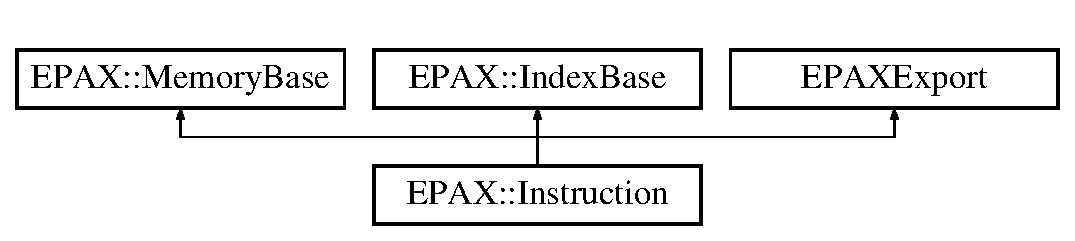
\includegraphics[height=2.000000cm]{class_e_p_a_x_1_1_instruction}
\end{center}
\end{figure}
\subsection*{\-Public \-Member \-Functions}
\begin{DoxyCompactItemize}
\item 
\hyperlink{class_e_p_a_x_1_1_instruction_a4e347d9655c0c4f3f9ea5a2168825d0c}{\-Instruction} (const uint64\-\_\-t a, const \hyperlink{_e_p_a_x_common_internal_8hpp_a17755bdd71c02e656c667b16de61dd7b}{rawbyte\-\_\-t} $\ast$r, \hyperlink{class_e_p_a_x_1_1_function}{\-Function} $\ast$func, const darm\-\_\-mode\-\_\-t mode)
\item 
virtual \hyperlink{class_e_p_a_x_1_1_instruction_acba01d9121bc060ee462d80cc34fc7fc}{$\sim$\-Instruction} ()
\item 
darm\-\_\-t $\ast$ \hyperlink{class_e_p_a_x_1_1_instruction_a890f727eb1f9fec8368af54cf8688b97}{source} ()
\item 
void \hyperlink{class_e_p_a_x_1_1_instruction_a38277ea3536685fc8f03fecd186302f8}{set\-Basic\-Block} (\hyperlink{class_e_p_a_x_1_1_basic_block}{\-Basic\-Block} $\ast$bb)
\item 
\hyperlink{class_e_p_a_x_1_1_basic_block}{\-Basic\-Block} $\ast$ \hyperlink{class_e_p_a_x_1_1_instruction_afeafa6b86ee4e118663439c907a5c89b}{get\-Basic\-Block} ()
\item 
darm\-\_\-cond\-\_\-t \hyperlink{class_e_p_a_x_1_1_instruction_a0571ec1274ce9c264b2091fb7d679986}{get\-Condition} ()
\item 
bool \hyperlink{class_e_p_a_x_1_1_instruction_af6355646396d8a907a27822f074cc677}{is\-Branch} ()
\item 
bool \hyperlink{class_e_p_a_x_1_1_instruction_a4e9f0285e1bc78ffb0ce120ba1644c8c}{is\-Conditional\-Branch} ()
\item 
bool \hyperlink{class_e_p_a_x_1_1_instruction_aa2262112acef930a6bab1c5d37651486}{is\-Unconditional\-Branch} ()
\item 
bool \hyperlink{class_e_p_a_x_1_1_instruction_a42bc25733ce0d1095c0235d75fe22d77}{has\-Fallthrough} ()
\item 
bool \hyperlink{class_e_p_a_x_1_1_instruction_a0905e9164967ddbfa9b746676ed3e221}{touches\-P\-C} ()
\item 
bool \hyperlink{class_e_p_a_x_1_1_instruction_a75f19cced51e7904d97e7f3224a40279}{is\-Call} ()
\item 
uint64\-\_\-t \hyperlink{class_e_p_a_x_1_1_instruction_a4d78a9d0f7ab52c678f3ff52a411eed6}{fallthrough\-Target} ()
\item 
uint64\-\_\-t \hyperlink{class_e_p_a_x_1_1_instruction_a8571ae62b9e8a2a24b6f063eff68902e}{get\-Branch\-Target} ()
\item 
uint32\-\_\-t \hyperlink{class_e_p_a_x_1_1_instruction_ab534268df34959940b11e31eb0473f00}{get\-Control\-Targets} (std\-::vector$<$ uint64\-\_\-t $>$ \&tgts)
\item 
bool \hyperlink{class_e_p_a_x_1_1_instruction_a6c4f718fb43f948b0ddfea2e79bee122}{is\-Fpop} ()
\item 
bool \hyperlink{class_e_p_a_x_1_1_instruction_a40207280f01d8a7f28527f6f85381b79}{is\-Load} ()
\item 
bool \hyperlink{class_e_p_a_x_1_1_instruction_a46a6b8fbab40247d8e9ff7c3f914b369}{is\-Store} ()
\item 
bool \hyperlink{class_e_p_a_x_1_1_instruction_a25c8f4fa7ad6296684fad26860f5719b}{is\-Memop} ()
\item 
uint32\-\_\-t \hyperlink{class_e_p_a_x_1_1_instruction_a971eef056f7df199d3ee902e33ce3ac1}{get\-Source\-Register\-Size\-In\-Bits} ()
\item 
uint32\-\_\-t \hyperlink{class_e_p_a_x_1_1_instruction_a863b17b7a11dd35b38ed72ba12e1a4a2}{get\-Source\-Datatype\-Size\-In\-Bits} ()
\item 
std\-::string \hyperlink{class_e_p_a_x_1_1_instruction_aa1e4422b1b5468ef2a6bc7ced4f93fc3}{string\-Rep} ()
\item 
void \hyperlink{class_e_p_a_x_1_1_instruction_aad46a5ae82142ed736ced45e9bf7d775}{print} (std\-::ostream \&stream=std\-::cout)
\end{DoxyCompactItemize}


\subsection{\-Detailed \-Description}


\-Definition at line 40 of file \-Instruction.\-hpp.



\subsection{\-Constructor \& \-Destructor \-Documentation}
\hypertarget{class_e_p_a_x_1_1_instruction_a4e347d9655c0c4f3f9ea5a2168825d0c}{\index{\-E\-P\-A\-X\-::\-Instruction@{\-E\-P\-A\-X\-::\-Instruction}!\-Instruction@{\-Instruction}}
\index{\-Instruction@{\-Instruction}!EPAX::Instruction@{\-E\-P\-A\-X\-::\-Instruction}}
\subsubsection[{\-Instruction}]{\setlength{\rightskip}{0pt plus 5cm}{\bf \-E\-P\-A\-X\-::\-Instruction\-::\-Instruction} (
\begin{DoxyParamCaption}
\item[{const uint64\-\_\-t}]{a, }
\item[{const {\bf rawbyte\-\_\-t} $\ast$}]{r, }
\item[{{\bf \-Function} $\ast$}]{func, }
\item[{const darm\-\_\-mode\-\_\-t}]{mode}
\end{DoxyParamCaption}
)}}\label{class_e_p_a_x_1_1_instruction_a4e347d9655c0c4f3f9ea5a2168825d0c}


\-Definition at line 38 of file \-Instruction.\-cpp.

\hypertarget{class_e_p_a_x_1_1_instruction_acba01d9121bc060ee462d80cc34fc7fc}{\index{\-E\-P\-A\-X\-::\-Instruction@{\-E\-P\-A\-X\-::\-Instruction}!$\sim$\-Instruction@{$\sim$\-Instruction}}
\index{$\sim$\-Instruction@{$\sim$\-Instruction}!EPAX::Instruction@{\-E\-P\-A\-X\-::\-Instruction}}
\subsubsection[{$\sim$\-Instruction}]{\setlength{\rightskip}{0pt plus 5cm}{\bf \-E\-P\-A\-X\-::\-Instruction\-::$\sim$\-Instruction} (
\begin{DoxyParamCaption}
{}
\end{DoxyParamCaption}
)\hspace{0.3cm}{\ttfamily  \mbox{[}virtual\mbox{]}}}}\label{class_e_p_a_x_1_1_instruction_acba01d9121bc060ee462d80cc34fc7fc}


\-Definition at line 106 of file \-Instruction.\-cpp.



\subsection{\-Member \-Function \-Documentation}
\hypertarget{class_e_p_a_x_1_1_instruction_a4d78a9d0f7ab52c678f3ff52a411eed6}{\index{\-E\-P\-A\-X\-::\-Instruction@{\-E\-P\-A\-X\-::\-Instruction}!fallthrough\-Target@{fallthrough\-Target}}
\index{fallthrough\-Target@{fallthrough\-Target}!EPAX::Instruction@{\-E\-P\-A\-X\-::\-Instruction}}
\subsubsection[{fallthrough\-Target}]{\setlength{\rightskip}{0pt plus 5cm}uint64\-\_\-t {\bf \-E\-P\-A\-X\-::\-Instruction\-::fallthrough\-Target} (
\begin{DoxyParamCaption}
{}
\end{DoxyParamCaption}
)}}\label{class_e_p_a_x_1_1_instruction_a4d78a9d0f7ab52c678f3ff52a411eed6}


\-Definition at line 257 of file \-Instruction.\-cpp.

\hypertarget{class_e_p_a_x_1_1_instruction_afeafa6b86ee4e118663439c907a5c89b}{\index{\-E\-P\-A\-X\-::\-Instruction@{\-E\-P\-A\-X\-::\-Instruction}!get\-Basic\-Block@{get\-Basic\-Block}}
\index{get\-Basic\-Block@{get\-Basic\-Block}!EPAX::Instruction@{\-E\-P\-A\-X\-::\-Instruction}}
\subsubsection[{get\-Basic\-Block}]{\setlength{\rightskip}{0pt plus 5cm}{\bf \-Basic\-Block}$\ast$ {\bf \-E\-P\-A\-X\-::\-Instruction\-::get\-Basic\-Block} (
\begin{DoxyParamCaption}
{}
\end{DoxyParamCaption}
)\hspace{0.3cm}{\ttfamily  \mbox{[}inline\mbox{]}}}}\label{class_e_p_a_x_1_1_instruction_afeafa6b86ee4e118663439c907a5c89b}


\-Definition at line 55 of file \-Instruction.\-hpp.

\hypertarget{class_e_p_a_x_1_1_instruction_a8571ae62b9e8a2a24b6f063eff68902e}{\index{\-E\-P\-A\-X\-::\-Instruction@{\-E\-P\-A\-X\-::\-Instruction}!get\-Branch\-Target@{get\-Branch\-Target}}
\index{get\-Branch\-Target@{get\-Branch\-Target}!EPAX::Instruction@{\-E\-P\-A\-X\-::\-Instruction}}
\subsubsection[{get\-Branch\-Target}]{\setlength{\rightskip}{0pt plus 5cm}uint64\-\_\-t {\bf \-E\-P\-A\-X\-::\-Instruction\-::get\-Branch\-Target} (
\begin{DoxyParamCaption}
{}
\end{DoxyParamCaption}
)}}\label{class_e_p_a_x_1_1_instruction_a8571ae62b9e8a2a24b6f063eff68902e}


\-Definition at line 217 of file \-Instruction.\-cpp.

\hypertarget{class_e_p_a_x_1_1_instruction_a0571ec1274ce9c264b2091fb7d679986}{\index{\-E\-P\-A\-X\-::\-Instruction@{\-E\-P\-A\-X\-::\-Instruction}!get\-Condition@{get\-Condition}}
\index{get\-Condition@{get\-Condition}!EPAX::Instruction@{\-E\-P\-A\-X\-::\-Instruction}}
\subsubsection[{get\-Condition}]{\setlength{\rightskip}{0pt plus 5cm}darm\-\_\-cond\-\_\-t {\bf \-E\-P\-A\-X\-::\-Instruction\-::get\-Condition} (
\begin{DoxyParamCaption}
{}
\end{DoxyParamCaption}
)}}\label{class_e_p_a_x_1_1_instruction_a0571ec1274ce9c264b2091fb7d679986}


\-Definition at line 117 of file \-Instruction.\-cpp.

\hypertarget{class_e_p_a_x_1_1_instruction_ab534268df34959940b11e31eb0473f00}{\index{\-E\-P\-A\-X\-::\-Instruction@{\-E\-P\-A\-X\-::\-Instruction}!get\-Control\-Targets@{get\-Control\-Targets}}
\index{get\-Control\-Targets@{get\-Control\-Targets}!EPAX::Instruction@{\-E\-P\-A\-X\-::\-Instruction}}
\subsubsection[{get\-Control\-Targets}]{\setlength{\rightskip}{0pt plus 5cm}uint32\-\_\-t {\bf \-E\-P\-A\-X\-::\-Instruction\-::get\-Control\-Targets} (
\begin{DoxyParamCaption}
\item[{std\-::vector$<$ uint64\-\_\-t $>$ \&}]{tgts}
\end{DoxyParamCaption}
)}}\label{class_e_p_a_x_1_1_instruction_ab534268df34959940b11e31eb0473f00}


\-Definition at line 262 of file \-Instruction.\-cpp.

\hypertarget{class_e_p_a_x_1_1_instruction_a863b17b7a11dd35b38ed72ba12e1a4a2}{\index{\-E\-P\-A\-X\-::\-Instruction@{\-E\-P\-A\-X\-::\-Instruction}!get\-Source\-Datatype\-Size\-In\-Bits@{get\-Source\-Datatype\-Size\-In\-Bits}}
\index{get\-Source\-Datatype\-Size\-In\-Bits@{get\-Source\-Datatype\-Size\-In\-Bits}!EPAX::Instruction@{\-E\-P\-A\-X\-::\-Instruction}}
\subsubsection[{get\-Source\-Datatype\-Size\-In\-Bits}]{\setlength{\rightskip}{0pt plus 5cm}uint32\-\_\-t {\bf \-E\-P\-A\-X\-::\-Instruction\-::get\-Source\-Datatype\-Size\-In\-Bits} (
\begin{DoxyParamCaption}
{}
\end{DoxyParamCaption}
)}}\label{class_e_p_a_x_1_1_instruction_a863b17b7a11dd35b38ed72ba12e1a4a2}


\-Definition at line 351 of file \-Instruction.\-cpp.

\hypertarget{class_e_p_a_x_1_1_instruction_a971eef056f7df199d3ee902e33ce3ac1}{\index{\-E\-P\-A\-X\-::\-Instruction@{\-E\-P\-A\-X\-::\-Instruction}!get\-Source\-Register\-Size\-In\-Bits@{get\-Source\-Register\-Size\-In\-Bits}}
\index{get\-Source\-Register\-Size\-In\-Bits@{get\-Source\-Register\-Size\-In\-Bits}!EPAX::Instruction@{\-E\-P\-A\-X\-::\-Instruction}}
\subsubsection[{get\-Source\-Register\-Size\-In\-Bits}]{\setlength{\rightskip}{0pt plus 5cm}uint32\-\_\-t {\bf \-E\-P\-A\-X\-::\-Instruction\-::get\-Source\-Register\-Size\-In\-Bits} (
\begin{DoxyParamCaption}
{}
\end{DoxyParamCaption}
)}}\label{class_e_p_a_x_1_1_instruction_a971eef056f7df199d3ee902e33ce3ac1}


\-Definition at line 335 of file \-Instruction.\-cpp.

\hypertarget{class_e_p_a_x_1_1_instruction_a42bc25733ce0d1095c0235d75fe22d77}{\index{\-E\-P\-A\-X\-::\-Instruction@{\-E\-P\-A\-X\-::\-Instruction}!has\-Fallthrough@{has\-Fallthrough}}
\index{has\-Fallthrough@{has\-Fallthrough}!EPAX::Instruction@{\-E\-P\-A\-X\-::\-Instruction}}
\subsubsection[{has\-Fallthrough}]{\setlength{\rightskip}{0pt plus 5cm}bool {\bf \-E\-P\-A\-X\-::\-Instruction\-::has\-Fallthrough} (
\begin{DoxyParamCaption}
{}
\end{DoxyParamCaption}
)}}\label{class_e_p_a_x_1_1_instruction_a42bc25733ce0d1095c0235d75fe22d77}


\-Definition at line 244 of file \-Instruction.\-cpp.

\hypertarget{class_e_p_a_x_1_1_instruction_af6355646396d8a907a27822f074cc677}{\index{\-E\-P\-A\-X\-::\-Instruction@{\-E\-P\-A\-X\-::\-Instruction}!is\-Branch@{is\-Branch}}
\index{is\-Branch@{is\-Branch}!EPAX::Instruction@{\-E\-P\-A\-X\-::\-Instruction}}
\subsubsection[{is\-Branch}]{\setlength{\rightskip}{0pt plus 5cm}bool {\bf \-E\-P\-A\-X\-::\-Instruction\-::is\-Branch} (
\begin{DoxyParamCaption}
{}
\end{DoxyParamCaption}
)}}\label{class_e_p_a_x_1_1_instruction_af6355646396d8a907a27822f074cc677}


\-Definition at line 175 of file \-Instruction.\-cpp.

\hypertarget{class_e_p_a_x_1_1_instruction_a75f19cced51e7904d97e7f3224a40279}{\index{\-E\-P\-A\-X\-::\-Instruction@{\-E\-P\-A\-X\-::\-Instruction}!is\-Call@{is\-Call}}
\index{is\-Call@{is\-Call}!EPAX::Instruction@{\-E\-P\-A\-X\-::\-Instruction}}
\subsubsection[{is\-Call}]{\setlength{\rightskip}{0pt plus 5cm}bool {\bf \-E\-P\-A\-X\-::\-Instruction\-::is\-Call} (
\begin{DoxyParamCaption}
{}
\end{DoxyParamCaption}
)}}\label{class_e_p_a_x_1_1_instruction_a75f19cced51e7904d97e7f3224a40279}


\-Definition at line 209 of file \-Instruction.\-cpp.

\hypertarget{class_e_p_a_x_1_1_instruction_a4e9f0285e1bc78ffb0ce120ba1644c8c}{\index{\-E\-P\-A\-X\-::\-Instruction@{\-E\-P\-A\-X\-::\-Instruction}!is\-Conditional\-Branch@{is\-Conditional\-Branch}}
\index{is\-Conditional\-Branch@{is\-Conditional\-Branch}!EPAX::Instruction@{\-E\-P\-A\-X\-::\-Instruction}}
\subsubsection[{is\-Conditional\-Branch}]{\setlength{\rightskip}{0pt plus 5cm}bool {\bf \-E\-P\-A\-X\-::\-Instruction\-::is\-Conditional\-Branch} (
\begin{DoxyParamCaption}
{}
\end{DoxyParamCaption}
)}}\label{class_e_p_a_x_1_1_instruction_a4e9f0285e1bc78ffb0ce120ba1644c8c}


\-Definition at line 179 of file \-Instruction.\-cpp.

\hypertarget{class_e_p_a_x_1_1_instruction_a6c4f718fb43f948b0ddfea2e79bee122}{\index{\-E\-P\-A\-X\-::\-Instruction@{\-E\-P\-A\-X\-::\-Instruction}!is\-Fpop@{is\-Fpop}}
\index{is\-Fpop@{is\-Fpop}!EPAX::Instruction@{\-E\-P\-A\-X\-::\-Instruction}}
\subsubsection[{is\-Fpop}]{\setlength{\rightskip}{0pt plus 5cm}bool {\bf \-E\-P\-A\-X\-::\-Instruction\-::is\-Fpop} (
\begin{DoxyParamCaption}
{}
\end{DoxyParamCaption}
)}}\label{class_e_p_a_x_1_1_instruction_a6c4f718fb43f948b0ddfea2e79bee122}


\-Definition at line 273 of file \-Instruction.\-cpp.

\hypertarget{class_e_p_a_x_1_1_instruction_a40207280f01d8a7f28527f6f85381b79}{\index{\-E\-P\-A\-X\-::\-Instruction@{\-E\-P\-A\-X\-::\-Instruction}!is\-Load@{is\-Load}}
\index{is\-Load@{is\-Load}!EPAX::Instruction@{\-E\-P\-A\-X\-::\-Instruction}}
\subsubsection[{is\-Load}]{\setlength{\rightskip}{0pt plus 5cm}bool {\bf \-E\-P\-A\-X\-::\-Instruction\-::is\-Load} (
\begin{DoxyParamCaption}
{}
\end{DoxyParamCaption}
)}}\label{class_e_p_a_x_1_1_instruction_a40207280f01d8a7f28527f6f85381b79}


\-Definition at line 293 of file \-Instruction.\-cpp.

\hypertarget{class_e_p_a_x_1_1_instruction_a25c8f4fa7ad6296684fad26860f5719b}{\index{\-E\-P\-A\-X\-::\-Instruction@{\-E\-P\-A\-X\-::\-Instruction}!is\-Memop@{is\-Memop}}
\index{is\-Memop@{is\-Memop}!EPAX::Instruction@{\-E\-P\-A\-X\-::\-Instruction}}
\subsubsection[{is\-Memop}]{\setlength{\rightskip}{0pt plus 5cm}bool {\bf \-E\-P\-A\-X\-::\-Instruction\-::is\-Memop} (
\begin{DoxyParamCaption}
{}
\end{DoxyParamCaption}
)}}\label{class_e_p_a_x_1_1_instruction_a25c8f4fa7ad6296684fad26860f5719b}


\-Definition at line 331 of file \-Instruction.\-cpp.

\hypertarget{class_e_p_a_x_1_1_instruction_a46a6b8fbab40247d8e9ff7c3f914b369}{\index{\-E\-P\-A\-X\-::\-Instruction@{\-E\-P\-A\-X\-::\-Instruction}!is\-Store@{is\-Store}}
\index{is\-Store@{is\-Store}!EPAX::Instruction@{\-E\-P\-A\-X\-::\-Instruction}}
\subsubsection[{is\-Store}]{\setlength{\rightskip}{0pt plus 5cm}bool {\bf \-E\-P\-A\-X\-::\-Instruction\-::is\-Store} (
\begin{DoxyParamCaption}
{}
\end{DoxyParamCaption}
)}}\label{class_e_p_a_x_1_1_instruction_a46a6b8fbab40247d8e9ff7c3f914b369}


\-Definition at line 312 of file \-Instruction.\-cpp.

\hypertarget{class_e_p_a_x_1_1_instruction_aa2262112acef930a6bab1c5d37651486}{\index{\-E\-P\-A\-X\-::\-Instruction@{\-E\-P\-A\-X\-::\-Instruction}!is\-Unconditional\-Branch@{is\-Unconditional\-Branch}}
\index{is\-Unconditional\-Branch@{is\-Unconditional\-Branch}!EPAX::Instruction@{\-E\-P\-A\-X\-::\-Instruction}}
\subsubsection[{is\-Unconditional\-Branch}]{\setlength{\rightskip}{0pt plus 5cm}bool {\bf \-E\-P\-A\-X\-::\-Instruction\-::is\-Unconditional\-Branch} (
\begin{DoxyParamCaption}
{}
\end{DoxyParamCaption}
)}}\label{class_e_p_a_x_1_1_instruction_aa2262112acef930a6bab1c5d37651486}


\-Definition at line 202 of file \-Instruction.\-cpp.

\hypertarget{class_e_p_a_x_1_1_instruction_aad46a5ae82142ed736ced45e9bf7d775}{\index{\-E\-P\-A\-X\-::\-Instruction@{\-E\-P\-A\-X\-::\-Instruction}!print@{print}}
\index{print@{print}!EPAX::Instruction@{\-E\-P\-A\-X\-::\-Instruction}}
\subsubsection[{print}]{\setlength{\rightskip}{0pt plus 5cm}void {\bf \-E\-P\-A\-X\-::\-Instruction\-::print} (
\begin{DoxyParamCaption}
\item[{std\-::ostream \&}]{stream = {\ttfamily std\-:\-:cout}}
\end{DoxyParamCaption}
)}}\label{class_e_p_a_x_1_1_instruction_aad46a5ae82142ed736ced45e9bf7d775}


\-Definition at line 121 of file \-Instruction.\-cpp.

\hypertarget{class_e_p_a_x_1_1_instruction_a38277ea3536685fc8f03fecd186302f8}{\index{\-E\-P\-A\-X\-::\-Instruction@{\-E\-P\-A\-X\-::\-Instruction}!set\-Basic\-Block@{set\-Basic\-Block}}
\index{set\-Basic\-Block@{set\-Basic\-Block}!EPAX::Instruction@{\-E\-P\-A\-X\-::\-Instruction}}
\subsubsection[{set\-Basic\-Block}]{\setlength{\rightskip}{0pt plus 5cm}void {\bf \-E\-P\-A\-X\-::\-Instruction\-::set\-Basic\-Block} (
\begin{DoxyParamCaption}
\item[{{\bf \-Basic\-Block} $\ast$}]{bb}
\end{DoxyParamCaption}
)\hspace{0.3cm}{\ttfamily  \mbox{[}inline\mbox{]}}}}\label{class_e_p_a_x_1_1_instruction_a38277ea3536685fc8f03fecd186302f8}


\-Definition at line 54 of file \-Instruction.\-hpp.

\hypertarget{class_e_p_a_x_1_1_instruction_a890f727eb1f9fec8368af54cf8688b97}{\index{\-E\-P\-A\-X\-::\-Instruction@{\-E\-P\-A\-X\-::\-Instruction}!source@{source}}
\index{source@{source}!EPAX::Instruction@{\-E\-P\-A\-X\-::\-Instruction}}
\subsubsection[{source}]{\setlength{\rightskip}{0pt plus 5cm}darm\-\_\-t$\ast$ {\bf \-E\-P\-A\-X\-::\-Instruction\-::source} (
\begin{DoxyParamCaption}
{}
\end{DoxyParamCaption}
)\hspace{0.3cm}{\ttfamily  \mbox{[}inline\mbox{]}}}}\label{class_e_p_a_x_1_1_instruction_a890f727eb1f9fec8368af54cf8688b97}


\-Definition at line 52 of file \-Instruction.\-hpp.

\hypertarget{class_e_p_a_x_1_1_instruction_aa1e4422b1b5468ef2a6bc7ced4f93fc3}{\index{\-E\-P\-A\-X\-::\-Instruction@{\-E\-P\-A\-X\-::\-Instruction}!string\-Rep@{string\-Rep}}
\index{string\-Rep@{string\-Rep}!EPAX::Instruction@{\-E\-P\-A\-X\-::\-Instruction}}
\subsubsection[{string\-Rep}]{\setlength{\rightskip}{0pt plus 5cm}std\-::string {\bf \-E\-P\-A\-X\-::\-Instruction\-::string\-Rep} (
\begin{DoxyParamCaption}
{}
\end{DoxyParamCaption}
)}}\label{class_e_p_a_x_1_1_instruction_aa1e4422b1b5468ef2a6bc7ced4f93fc3}


\-Definition at line 109 of file \-Instruction.\-cpp.

\hypertarget{class_e_p_a_x_1_1_instruction_a0905e9164967ddbfa9b746676ed3e221}{\index{\-E\-P\-A\-X\-::\-Instruction@{\-E\-P\-A\-X\-::\-Instruction}!touches\-P\-C@{touches\-P\-C}}
\index{touches\-P\-C@{touches\-P\-C}!EPAX::Instruction@{\-E\-P\-A\-X\-::\-Instruction}}
\subsubsection[{touches\-P\-C}]{\setlength{\rightskip}{0pt plus 5cm}bool {\bf \-E\-P\-A\-X\-::\-Instruction\-::touches\-P\-C} (
\begin{DoxyParamCaption}
{}
\end{DoxyParamCaption}
)}}\label{class_e_p_a_x_1_1_instruction_a0905e9164967ddbfa9b746676ed3e221}


\-Definition at line 186 of file \-Instruction.\-cpp.



\-The documentation for this class was generated from the following files\-:\begin{DoxyCompactItemize}
\item 
\hyperlink{_instruction_8hpp}{\-Instruction.\-hpp}\item 
\hyperlink{_instruction_8cpp}{\-Instruction.\-cpp}\end{DoxyCompactItemize}

\hypertarget{class_e_p_a_x_1_1_loop}{\section{\-E\-P\-A\-X\-:\-:\-Loop \-Class \-Reference}
\label{class_e_p_a_x_1_1_loop}\index{\-E\-P\-A\-X\-::\-Loop@{\-E\-P\-A\-X\-::\-Loop}}
}


{\ttfamily \#include $<$\-Loop.\-hpp$>$}

\-Inheritance diagram for \-E\-P\-A\-X\-:\-:\-Loop\-:\begin{figure}[H]
\begin{center}
\leavevmode
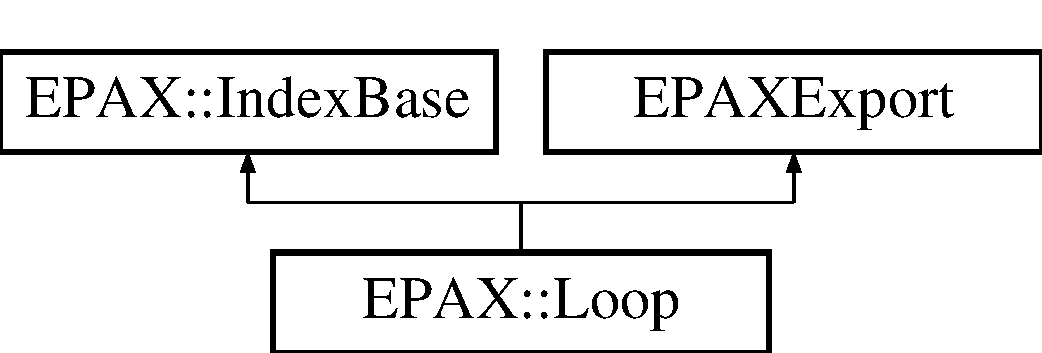
\includegraphics[height=2.000000cm]{class_e_p_a_x_1_1_loop}
\end{center}
\end{figure}
\subsection*{\-Public \-Member \-Functions}
\begin{DoxyCompactItemize}
\item 
\hyperlink{class_e_p_a_x_1_1_loop_a2bae87ec3d967c7bd70300687723c327}{\-Loop} (\hyperlink{class_e_p_a_x_1_1_control_flow}{\-Control\-Flow} $\ast$c, uint32\-\_\-t h, uint32\-\_\-t t, uint32\-\_\-t d, \hyperlink{class_e_p_a_x_1_1dyn__bitset}{dyn\-\_\-bitset} $\ast$m, uint32\-\_\-t i)
\item 
virtual \hyperlink{class_e_p_a_x_1_1_loop_a4e3bd5964896020904db2cc76cae55fb}{$\sim$\-Loop} ()
\item 
\hyperlink{class_e_p_a_x_1_1_control_flow}{\-Control\-Flow} $\ast$ \hyperlink{class_e_p_a_x_1_1_loop_aaace2fef9ea1eb09918ecb56017da0a2}{get\-Control\-Flow} ()
\item 
uint32\-\_\-t \hyperlink{class_e_p_a_x_1_1_loop_a70b6e7c9894ab1984df350d155cd20e1}{count\-Basic\-Blocks} ()
\item 
uint32\-\_\-t \hyperlink{class_e_p_a_x_1_1_loop_a54ac86da0c06049b8af6c6128e96fdca}{count\-Instructions} ()
\item 
uint32\-\_\-t \hyperlink{class_e_p_a_x_1_1_loop_a4c4c2097f1cb528e553ae7e6d75b9b14}{get\-Size} ()
\item 
\hyperlink{class_e_p_a_x_1_1_basic_block}{\-Basic\-Block} $\ast$ \hyperlink{class_e_p_a_x_1_1_loop_ad6b1a8c5fc295c42de1996658150c5f5}{find\-Basic\-Block} (uint64\-\_\-t addr)
\item 
bool \hyperlink{class_e_p_a_x_1_1_loop_ab22ae5ef44f2e033fb5d4ced1d72734d}{has\-Basic\-Block} (uint32\-\_\-t idx)
\item 
\hyperlink{class_e_p_a_x_1_1_basic_block}{\-Basic\-Block} $\ast$ \hyperlink{class_e_p_a_x_1_1_loop_a4f64475b12d85dbee8cb207903eb0b3b}{get\-Basic\-Block} (uint32\-\_\-t idx)
\item 
\hyperlink{class_e_p_a_x_1_1_basic_block}{\-Basic\-Block} $\ast$ \hyperlink{class_e_p_a_x_1_1_loop_abad7041e4d159472e14fcd0900510581}{get\-Next\-Basic\-Block} (uint32\-\_\-t idx)
\item 
bool \hyperlink{class_e_p_a_x_1_1_loop_adef4258c1ff9bde98a568bb5a0398be8}{is\-Last\-Basic\-Block} (uint32\-\_\-t idx)
\item 
\hyperlink{class_e_p_a_x_1_1_basic_block}{\-Basic\-Block} $\ast$ \hyperlink{class_e_p_a_x_1_1_loop_ab5a3d377e2da69fe6822dbf66a7390cd}{head} ()
\item 
\hyperlink{class_e_p_a_x_1_1_basic_block}{\-Basic\-Block} $\ast$ \hyperlink{class_e_p_a_x_1_1_loop_a5cecf77effc28550c9978371b113b6cb}{tail} ()
\item 
\hyperlink{class_e_p_a_x_1_1_instruction}{\-Instruction} $\ast$ \hyperlink{class_e_p_a_x_1_1_loop_ae44e1bd79a213b3b5873d24164d55623}{find\-Instruction} (uint64\-\_\-t addr)
\item 
\hyperlink{class_e_p_a_x_1_1_instruction}{\-Instruction} $\ast$ \hyperlink{class_e_p_a_x_1_1_loop_a2c75eef1d286f9d35800e668414a7950}{get\-Instruction} (uint32\-\_\-t idx)
\item 
bool \hyperlink{class_e_p_a_x_1_1_loop_a03aa2ad89a7b73560803f4e482fec5de}{is\-Last\-Instruction} (uint32\-\_\-t idx)
\item 
void \hyperlink{class_e_p_a_x_1_1_loop_ad361e0d0fc5b10185c84de493524f255}{set\-Depth} (uint32\-\_\-t d)
\item 
uint32\-\_\-t \hyperlink{class_e_p_a_x_1_1_loop_adbc0df439a7dfc5957a8850a041f0b34}{get\-Depth} ()
\item 
bool \hyperlink{class_e_p_a_x_1_1_loop_a9a2c4a4fd37713d66b55095191aa0b35}{is\-Child\-Of} (\hyperlink{class_e_p_a_x_1_1_loop}{\-Loop} $\ast$lp)
\end{DoxyCompactItemize}


\subsection{\-Detailed \-Description}


\-Definition at line 37 of file \-Loop.\-hpp.



\subsection{\-Constructor \& \-Destructor \-Documentation}
\hypertarget{class_e_p_a_x_1_1_loop_a2bae87ec3d967c7bd70300687723c327}{\index{\-E\-P\-A\-X\-::\-Loop@{\-E\-P\-A\-X\-::\-Loop}!\-Loop@{\-Loop}}
\index{\-Loop@{\-Loop}!EPAX::Loop@{\-E\-P\-A\-X\-::\-Loop}}
\subsubsection[{\-Loop}]{\setlength{\rightskip}{0pt plus 5cm}{\bf \-E\-P\-A\-X\-::\-Loop\-::\-Loop} (
\begin{DoxyParamCaption}
\item[{{\bf \-Control\-Flow} $\ast$}]{c, }
\item[{uint32\-\_\-t}]{h, }
\item[{uint32\-\_\-t}]{t, }
\item[{uint32\-\_\-t}]{d, }
\item[{{\bf dyn\-\_\-bitset} $\ast$}]{m, }
\item[{uint32\-\_\-t}]{i}
\end{DoxyParamCaption}
)}}\label{class_e_p_a_x_1_1_loop_a2bae87ec3d967c7bd70300687723c327}


\-Definition at line 34 of file \-Loop.\-cpp.

\hypertarget{class_e_p_a_x_1_1_loop_a4e3bd5964896020904db2cc76cae55fb}{\index{\-E\-P\-A\-X\-::\-Loop@{\-E\-P\-A\-X\-::\-Loop}!$\sim$\-Loop@{$\sim$\-Loop}}
\index{$\sim$\-Loop@{$\sim$\-Loop}!EPAX::Loop@{\-E\-P\-A\-X\-::\-Loop}}
\subsubsection[{$\sim$\-Loop}]{\setlength{\rightskip}{0pt plus 5cm}{\bf \-E\-P\-A\-X\-::\-Loop\-::$\sim$\-Loop} (
\begin{DoxyParamCaption}
{}
\end{DoxyParamCaption}
)\hspace{0.3cm}{\ttfamily  \mbox{[}virtual\mbox{]}}}}\label{class_e_p_a_x_1_1_loop_a4e3bd5964896020904db2cc76cae55fb}


\-Definition at line 50 of file \-Loop.\-cpp.



\subsection{\-Member \-Function \-Documentation}
\hypertarget{class_e_p_a_x_1_1_loop_a70b6e7c9894ab1984df350d155cd20e1}{\index{\-E\-P\-A\-X\-::\-Loop@{\-E\-P\-A\-X\-::\-Loop}!count\-Basic\-Blocks@{count\-Basic\-Blocks}}
\index{count\-Basic\-Blocks@{count\-Basic\-Blocks}!EPAX::Loop@{\-E\-P\-A\-X\-::\-Loop}}
\subsubsection[{count\-Basic\-Blocks}]{\setlength{\rightskip}{0pt plus 5cm}uint32\-\_\-t {\bf \-E\-P\-A\-X\-::\-Loop\-::count\-Basic\-Blocks} (
\begin{DoxyParamCaption}
{}
\end{DoxyParamCaption}
)}}\label{class_e_p_a_x_1_1_loop_a70b6e7c9894ab1984df350d155cd20e1}


\-Definition at line 98 of file \-Loop.\-cpp.

\hypertarget{class_e_p_a_x_1_1_loop_a54ac86da0c06049b8af6c6128e96fdca}{\index{\-E\-P\-A\-X\-::\-Loop@{\-E\-P\-A\-X\-::\-Loop}!count\-Instructions@{count\-Instructions}}
\index{count\-Instructions@{count\-Instructions}!EPAX::Loop@{\-E\-P\-A\-X\-::\-Loop}}
\subsubsection[{count\-Instructions}]{\setlength{\rightskip}{0pt plus 5cm}uint32\-\_\-t {\bf \-E\-P\-A\-X\-::\-Loop\-::count\-Instructions} (
\begin{DoxyParamCaption}
{}
\end{DoxyParamCaption}
)}}\label{class_e_p_a_x_1_1_loop_a54ac86da0c06049b8af6c6128e96fdca}


\-Definition at line 86 of file \-Loop.\-cpp.

\hypertarget{class_e_p_a_x_1_1_loop_ad6b1a8c5fc295c42de1996658150c5f5}{\index{\-E\-P\-A\-X\-::\-Loop@{\-E\-P\-A\-X\-::\-Loop}!find\-Basic\-Block@{find\-Basic\-Block}}
\index{find\-Basic\-Block@{find\-Basic\-Block}!EPAX::Loop@{\-E\-P\-A\-X\-::\-Loop}}
\subsubsection[{find\-Basic\-Block}]{\setlength{\rightskip}{0pt plus 5cm}{\bf \-Basic\-Block} $\ast$ {\bf \-E\-P\-A\-X\-::\-Loop\-::find\-Basic\-Block} (
\begin{DoxyParamCaption}
\item[{uint64\-\_\-t}]{addr}
\end{DoxyParamCaption}
)}}\label{class_e_p_a_x_1_1_loop_ad6b1a8c5fc295c42de1996658150c5f5}


\-Definition at line 120 of file \-Loop.\-cpp.

\hypertarget{class_e_p_a_x_1_1_loop_ae44e1bd79a213b3b5873d24164d55623}{\index{\-E\-P\-A\-X\-::\-Loop@{\-E\-P\-A\-X\-::\-Loop}!find\-Instruction@{find\-Instruction}}
\index{find\-Instruction@{find\-Instruction}!EPAX::Loop@{\-E\-P\-A\-X\-::\-Loop}}
\subsubsection[{find\-Instruction}]{\setlength{\rightskip}{0pt plus 5cm}{\bf \-Instruction} $\ast$ {\bf \-E\-P\-A\-X\-::\-Loop\-::find\-Instruction} (
\begin{DoxyParamCaption}
\item[{uint64\-\_\-t}]{addr}
\end{DoxyParamCaption}
)}}\label{class_e_p_a_x_1_1_loop_ae44e1bd79a213b3b5873d24164d55623}


\-Definition at line 78 of file \-Loop.\-cpp.

\hypertarget{class_e_p_a_x_1_1_loop_a4f64475b12d85dbee8cb207903eb0b3b}{\index{\-E\-P\-A\-X\-::\-Loop@{\-E\-P\-A\-X\-::\-Loop}!get\-Basic\-Block@{get\-Basic\-Block}}
\index{get\-Basic\-Block@{get\-Basic\-Block}!EPAX::Loop@{\-E\-P\-A\-X\-::\-Loop}}
\subsubsection[{get\-Basic\-Block}]{\setlength{\rightskip}{0pt plus 5cm}{\bf \-Basic\-Block} $\ast$ {\bf \-E\-P\-A\-X\-::\-Loop\-::get\-Basic\-Block} (
\begin{DoxyParamCaption}
\item[{uint32\-\_\-t}]{idx}
\end{DoxyParamCaption}
)}}\label{class_e_p_a_x_1_1_loop_a4f64475b12d85dbee8cb207903eb0b3b}


\-Definition at line 139 of file \-Loop.\-cpp.

\hypertarget{class_e_p_a_x_1_1_loop_aaace2fef9ea1eb09918ecb56017da0a2}{\index{\-E\-P\-A\-X\-::\-Loop@{\-E\-P\-A\-X\-::\-Loop}!get\-Control\-Flow@{get\-Control\-Flow}}
\index{get\-Control\-Flow@{get\-Control\-Flow}!EPAX::Loop@{\-E\-P\-A\-X\-::\-Loop}}
\subsubsection[{get\-Control\-Flow}]{\setlength{\rightskip}{0pt plus 5cm}{\bf \-Control\-Flow}$\ast$ {\bf \-E\-P\-A\-X\-::\-Loop\-::get\-Control\-Flow} (
\begin{DoxyParamCaption}
{}
\end{DoxyParamCaption}
)\hspace{0.3cm}{\ttfamily  \mbox{[}inline\mbox{]}}}}\label{class_e_p_a_x_1_1_loop_aaace2fef9ea1eb09918ecb56017da0a2}


\-Definition at line 50 of file \-Loop.\-hpp.

\hypertarget{class_e_p_a_x_1_1_loop_adbc0df439a7dfc5957a8850a041f0b34}{\index{\-E\-P\-A\-X\-::\-Loop@{\-E\-P\-A\-X\-::\-Loop}!get\-Depth@{get\-Depth}}
\index{get\-Depth@{get\-Depth}!EPAX::Loop@{\-E\-P\-A\-X\-::\-Loop}}
\subsubsection[{get\-Depth}]{\setlength{\rightskip}{0pt plus 5cm}uint32\-\_\-t {\bf \-E\-P\-A\-X\-::\-Loop\-::get\-Depth} (
\begin{DoxyParamCaption}
{}
\end{DoxyParamCaption}
)}}\label{class_e_p_a_x_1_1_loop_adbc0df439a7dfc5957a8850a041f0b34}


\-Definition at line 201 of file \-Loop.\-cpp.

\hypertarget{class_e_p_a_x_1_1_loop_a2c75eef1d286f9d35800e668414a7950}{\index{\-E\-P\-A\-X\-::\-Loop@{\-E\-P\-A\-X\-::\-Loop}!get\-Instruction@{get\-Instruction}}
\index{get\-Instruction@{get\-Instruction}!EPAX::Loop@{\-E\-P\-A\-X\-::\-Loop}}
\subsubsection[{get\-Instruction}]{\setlength{\rightskip}{0pt plus 5cm}{\bf \-Instruction}$\ast$ {\bf \-E\-P\-A\-X\-::\-Loop\-::get\-Instruction} (
\begin{DoxyParamCaption}
\item[{uint32\-\_\-t}]{idx}
\end{DoxyParamCaption}
)}}\label{class_e_p_a_x_1_1_loop_a2c75eef1d286f9d35800e668414a7950}
\hypertarget{class_e_p_a_x_1_1_loop_abad7041e4d159472e14fcd0900510581}{\index{\-E\-P\-A\-X\-::\-Loop@{\-E\-P\-A\-X\-::\-Loop}!get\-Next\-Basic\-Block@{get\-Next\-Basic\-Block}}
\index{get\-Next\-Basic\-Block@{get\-Next\-Basic\-Block}!EPAX::Loop@{\-E\-P\-A\-X\-::\-Loop}}
\subsubsection[{get\-Next\-Basic\-Block}]{\setlength{\rightskip}{0pt plus 5cm}{\bf \-Basic\-Block} $\ast$ {\bf \-E\-P\-A\-X\-::\-Loop\-::get\-Next\-Basic\-Block} (
\begin{DoxyParamCaption}
\item[{uint32\-\_\-t}]{idx}
\end{DoxyParamCaption}
)}}\label{class_e_p_a_x_1_1_loop_abad7041e4d159472e14fcd0900510581}


\-Definition at line 149 of file \-Loop.\-cpp.

\hypertarget{class_e_p_a_x_1_1_loop_a4c4c2097f1cb528e553ae7e6d75b9b14}{\index{\-E\-P\-A\-X\-::\-Loop@{\-E\-P\-A\-X\-::\-Loop}!get\-Size@{get\-Size}}
\index{get\-Size@{get\-Size}!EPAX::Loop@{\-E\-P\-A\-X\-::\-Loop}}
\subsubsection[{get\-Size}]{\setlength{\rightskip}{0pt plus 5cm}uint32\-\_\-t {\bf \-E\-P\-A\-X\-::\-Loop\-::get\-Size} (
\begin{DoxyParamCaption}
{}
\end{DoxyParamCaption}
)}}\label{class_e_p_a_x_1_1_loop_a4c4c2097f1cb528e553ae7e6d75b9b14}


\-Definition at line 108 of file \-Loop.\-cpp.

\hypertarget{class_e_p_a_x_1_1_loop_ab22ae5ef44f2e033fb5d4ced1d72734d}{\index{\-E\-P\-A\-X\-::\-Loop@{\-E\-P\-A\-X\-::\-Loop}!has\-Basic\-Block@{has\-Basic\-Block}}
\index{has\-Basic\-Block@{has\-Basic\-Block}!EPAX::Loop@{\-E\-P\-A\-X\-::\-Loop}}
\subsubsection[{has\-Basic\-Block}]{\setlength{\rightskip}{0pt plus 5cm}bool {\bf \-E\-P\-A\-X\-::\-Loop\-::has\-Basic\-Block} (
\begin{DoxyParamCaption}
\item[{uint32\-\_\-t}]{idx}
\end{DoxyParamCaption}
)}}\label{class_e_p_a_x_1_1_loop_ab22ae5ef44f2e033fb5d4ced1d72734d}


\-Definition at line 135 of file \-Loop.\-cpp.

\hypertarget{class_e_p_a_x_1_1_loop_ab5a3d377e2da69fe6822dbf66a7390cd}{\index{\-E\-P\-A\-X\-::\-Loop@{\-E\-P\-A\-X\-::\-Loop}!head@{head}}
\index{head@{head}!EPAX::Loop@{\-E\-P\-A\-X\-::\-Loop}}
\subsubsection[{head}]{\setlength{\rightskip}{0pt plus 5cm}{\bf \-Basic\-Block} $\ast$ {\bf \-E\-P\-A\-X\-::\-Loop\-::head} (
\begin{DoxyParamCaption}
{}
\end{DoxyParamCaption}
)}}\label{class_e_p_a_x_1_1_loop_ab5a3d377e2da69fe6822dbf66a7390cd}


\-Definition at line 56 of file \-Loop.\-cpp.

\hypertarget{class_e_p_a_x_1_1_loop_a9a2c4a4fd37713d66b55095191aa0b35}{\index{\-E\-P\-A\-X\-::\-Loop@{\-E\-P\-A\-X\-::\-Loop}!is\-Child\-Of@{is\-Child\-Of}}
\index{is\-Child\-Of@{is\-Child\-Of}!EPAX::Loop@{\-E\-P\-A\-X\-::\-Loop}}
\subsubsection[{is\-Child\-Of}]{\setlength{\rightskip}{0pt plus 5cm}bool {\bf \-E\-P\-A\-X\-::\-Loop\-::is\-Child\-Of} (
\begin{DoxyParamCaption}
\item[{{\bf \-Loop} $\ast$}]{lp}
\end{DoxyParamCaption}
)}}\label{class_e_p_a_x_1_1_loop_a9a2c4a4fd37713d66b55095191aa0b35}


\-Definition at line 182 of file \-Loop.\-cpp.

\hypertarget{class_e_p_a_x_1_1_loop_adef4258c1ff9bde98a568bb5a0398be8}{\index{\-E\-P\-A\-X\-::\-Loop@{\-E\-P\-A\-X\-::\-Loop}!is\-Last\-Basic\-Block@{is\-Last\-Basic\-Block}}
\index{is\-Last\-Basic\-Block@{is\-Last\-Basic\-Block}!EPAX::Loop@{\-E\-P\-A\-X\-::\-Loop}}
\subsubsection[{is\-Last\-Basic\-Block}]{\setlength{\rightskip}{0pt plus 5cm}bool {\bf \-E\-P\-A\-X\-::\-Loop\-::is\-Last\-Basic\-Block} (
\begin{DoxyParamCaption}
\item[{uint32\-\_\-t}]{idx}
\end{DoxyParamCaption}
)}}\label{class_e_p_a_x_1_1_loop_adef4258c1ff9bde98a568bb5a0398be8}


\-Definition at line 165 of file \-Loop.\-cpp.

\hypertarget{class_e_p_a_x_1_1_loop_a03aa2ad89a7b73560803f4e482fec5de}{\index{\-E\-P\-A\-X\-::\-Loop@{\-E\-P\-A\-X\-::\-Loop}!is\-Last\-Instruction@{is\-Last\-Instruction}}
\index{is\-Last\-Instruction@{is\-Last\-Instruction}!EPAX::Loop@{\-E\-P\-A\-X\-::\-Loop}}
\subsubsection[{is\-Last\-Instruction}]{\setlength{\rightskip}{0pt plus 5cm}bool {\bf \-E\-P\-A\-X\-::\-Loop\-::is\-Last\-Instruction} (
\begin{DoxyParamCaption}
\item[{uint32\-\_\-t}]{idx}
\end{DoxyParamCaption}
)}}\label{class_e_p_a_x_1_1_loop_a03aa2ad89a7b73560803f4e482fec5de}
\hypertarget{class_e_p_a_x_1_1_loop_ad361e0d0fc5b10185c84de493524f255}{\index{\-E\-P\-A\-X\-::\-Loop@{\-E\-P\-A\-X\-::\-Loop}!set\-Depth@{set\-Depth}}
\index{set\-Depth@{set\-Depth}!EPAX::Loop@{\-E\-P\-A\-X\-::\-Loop}}
\subsubsection[{set\-Depth}]{\setlength{\rightskip}{0pt plus 5cm}void {\bf \-E\-P\-A\-X\-::\-Loop\-::set\-Depth} (
\begin{DoxyParamCaption}
\item[{uint32\-\_\-t}]{d}
\end{DoxyParamCaption}
)}}\label{class_e_p_a_x_1_1_loop_ad361e0d0fc5b10185c84de493524f255}


\-Definition at line 197 of file \-Loop.\-cpp.

\hypertarget{class_e_p_a_x_1_1_loop_a5cecf77effc28550c9978371b113b6cb}{\index{\-E\-P\-A\-X\-::\-Loop@{\-E\-P\-A\-X\-::\-Loop}!tail@{tail}}
\index{tail@{tail}!EPAX::Loop@{\-E\-P\-A\-X\-::\-Loop}}
\subsubsection[{tail}]{\setlength{\rightskip}{0pt plus 5cm}{\bf \-Basic\-Block} $\ast$ {\bf \-E\-P\-A\-X\-::\-Loop\-::tail} (
\begin{DoxyParamCaption}
{}
\end{DoxyParamCaption}
)}}\label{class_e_p_a_x_1_1_loop_a5cecf77effc28550c9978371b113b6cb}


\-Definition at line 67 of file \-Loop.\-cpp.



\-The documentation for this class was generated from the following files\-:\begin{DoxyCompactItemize}
\item 
\hyperlink{_loop_8hpp}{\-Loop.\-hpp}\item 
\hyperlink{_loop_8cpp}{\-Loop.\-cpp}\end{DoxyCompactItemize}

\hypertarget{class_e_p_a_x_1_1_mach_o_1_1_mach_header}{\section{\-E\-P\-A\-X\-:\-:\-Mach\-O\-:\-:\-Mach\-Header \-Class \-Reference}
\label{class_e_p_a_x_1_1_mach_o_1_1_mach_header}\index{\-E\-P\-A\-X\-::\-Mach\-O\-::\-Mach\-Header@{\-E\-P\-A\-X\-::\-Mach\-O\-::\-Mach\-Header}}
}


{\ttfamily \#include $<$\-Mach\-O\-Binary.\-hpp$>$}

\-Inheritance diagram for \-E\-P\-A\-X\-:\-:\-Mach\-O\-:\-:\-Mach\-Header\-:\begin{figure}[H]
\begin{center}
\leavevmode
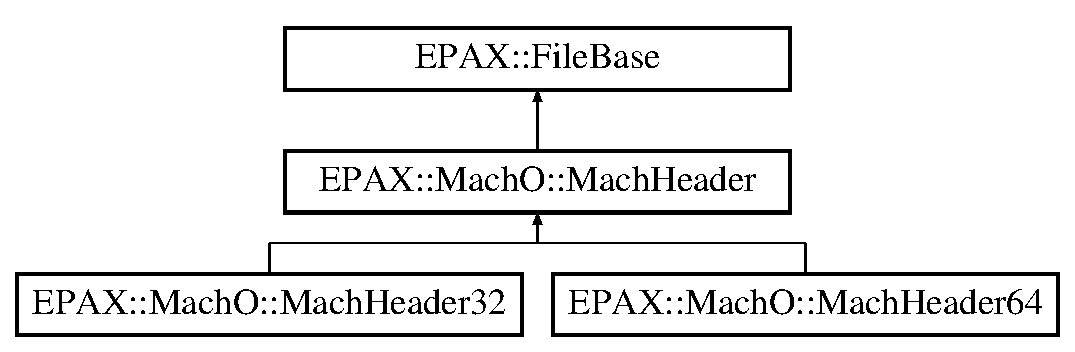
\includegraphics[height=3.000000cm]{class_e_p_a_x_1_1_mach_o_1_1_mach_header}
\end{center}
\end{figure}
\subsection*{\-Public \-Member \-Functions}
\begin{DoxyCompactItemize}
\item 
\hyperlink{class_e_p_a_x_1_1_mach_o_1_1_mach_header_a75491057ad159d2eb3f3a183ac7eecc9}{\-Mach\-Header} (\hyperlink{class_e_p_a_x_1_1_base_binary}{\-Base\-Binary} $\ast$b, uint64\-\_\-t o, uint64\-\_\-t s)
\item 
virtual \hyperlink{class_e_p_a_x_1_1_mach_o_1_1_mach_header_ae5338ee30e88a688edce08ec66094fa8}{$\sim$\-Mach\-Header} ()
\item 
virtual uint64\-\_\-t \hyperlink{class_e_p_a_x_1_1_mach_o_1_1_mach_header_aeae22d677b30ceeed55c7f7910a45ff1}{get\-Start\-Addr} ()=0
\item 
virtual bool \hyperlink{class_e_p_a_x_1_1_mach_o_1_1_mach_header_aeca0eb4432fece14fc5bb27810a63e06}{verify} ()=0
\item 
virtual bool \hyperlink{class_e_p_a_x_1_1_mach_o_1_1_mach_header_a95466e1612d0ad48d991830f4c3898ee}{is\-A\-R\-M} ()=0
\item 
virtual void \hyperlink{class_e_p_a_x_1_1_mach_o_1_1_mach_header_a6e04356c40b005cc7f9c8e318f327e2c}{describe} ()=0
\item 
virtual uint32\-\_\-t \hyperlink{class_e_p_a_x_1_1_mach_o_1_1_mach_header_a667362bbcc5a18b89b430c3bbf9dbcf3}{get\-File\-Type} ()=0
\end{DoxyCompactItemize}
\subsection*{\-Static \-Protected \-Member \-Functions}
\begin{DoxyCompactItemize}
\item 
static void \hyperlink{class_e_p_a_x_1_1_mach_o_1_1_mach_header_a7480abca8a0a85891f942d652db9cf52}{describe\-I\-S\-A} (int32\-\_\-t ctype, int32\-\_\-t stype)
\end{DoxyCompactItemize}
\subsection*{\-Protected \-Attributes}
\begin{DoxyCompactItemize}
\item 
\hyperlink{_e_p_a_x_common_internal_8hpp_a17755bdd71c02e656c667b16de61dd7b}{rawbyte\-\_\-t} $\ast$ \hyperlink{class_e_p_a_x_1_1_mach_o_1_1_mach_header_af181c13ccbaa856882bf648aa7fbe295}{entry}
\end{DoxyCompactItemize}


\subsection{\-Detailed \-Description}


\-Definition at line 85 of file \-Mach\-O\-Binary.\-hpp.



\subsection{\-Constructor \& \-Destructor \-Documentation}
\hypertarget{class_e_p_a_x_1_1_mach_o_1_1_mach_header_a75491057ad159d2eb3f3a183ac7eecc9}{\index{\-E\-P\-A\-X\-::\-Mach\-O\-::\-Mach\-Header@{\-E\-P\-A\-X\-::\-Mach\-O\-::\-Mach\-Header}!\-Mach\-Header@{\-Mach\-Header}}
\index{\-Mach\-Header@{\-Mach\-Header}!EPAX::MachO::MachHeader@{\-E\-P\-A\-X\-::\-Mach\-O\-::\-Mach\-Header}}
\subsubsection[{\-Mach\-Header}]{\setlength{\rightskip}{0pt plus 5cm}{\bf \-E\-P\-A\-X\-::\-Mach\-O\-::\-Mach\-Header\-::\-Mach\-Header} (
\begin{DoxyParamCaption}
\item[{{\bf \-Base\-Binary} $\ast$}]{b, }
\item[{uint64\-\_\-t}]{o, }
\item[{uint64\-\_\-t}]{s}
\end{DoxyParamCaption}
)}}\label{class_e_p_a_x_1_1_mach_o_1_1_mach_header_a75491057ad159d2eb3f3a183ac7eecc9}


\-Definition at line 119 of file \-Mach\-O\-Binary.\-cpp.

\hypertarget{class_e_p_a_x_1_1_mach_o_1_1_mach_header_ae5338ee30e88a688edce08ec66094fa8}{\index{\-E\-P\-A\-X\-::\-Mach\-O\-::\-Mach\-Header@{\-E\-P\-A\-X\-::\-Mach\-O\-::\-Mach\-Header}!$\sim$\-Mach\-Header@{$\sim$\-Mach\-Header}}
\index{$\sim$\-Mach\-Header@{$\sim$\-Mach\-Header}!EPAX::MachO::MachHeader@{\-E\-P\-A\-X\-::\-Mach\-O\-::\-Mach\-Header}}
\subsubsection[{$\sim$\-Mach\-Header}]{\setlength{\rightskip}{0pt plus 5cm}{\bf \-E\-P\-A\-X\-::\-Mach\-O\-::\-Mach\-Header\-::$\sim$\-Mach\-Header} (
\begin{DoxyParamCaption}
{}
\end{DoxyParamCaption}
)\hspace{0.3cm}{\ttfamily  \mbox{[}virtual\mbox{]}}}}\label{class_e_p_a_x_1_1_mach_o_1_1_mach_header_ae5338ee30e88a688edce08ec66094fa8}


\-Definition at line 125 of file \-Mach\-O\-Binary.\-cpp.



\subsection{\-Member \-Function \-Documentation}
\hypertarget{class_e_p_a_x_1_1_mach_o_1_1_mach_header_a6e04356c40b005cc7f9c8e318f327e2c}{\index{\-E\-P\-A\-X\-::\-Mach\-O\-::\-Mach\-Header@{\-E\-P\-A\-X\-::\-Mach\-O\-::\-Mach\-Header}!describe@{describe}}
\index{describe@{describe}!EPAX::MachO::MachHeader@{\-E\-P\-A\-X\-::\-Mach\-O\-::\-Mach\-Header}}
\subsubsection[{describe}]{\setlength{\rightskip}{0pt plus 5cm}void {\bf \-E\-P\-A\-X\-::\-Mach\-O\-::\-Mach\-Header\-::describe} (
\begin{DoxyParamCaption}
{}
\end{DoxyParamCaption}
)\hspace{0.3cm}{\ttfamily  \mbox{[}pure virtual\mbox{]}}}}\label{class_e_p_a_x_1_1_mach_o_1_1_mach_header_a6e04356c40b005cc7f9c8e318f327e2c}


\-Implemented in \hyperlink{class_e_p_a_x_1_1_mach_o_1_1_mach_header64_ad56f5abdcfd8bf2898d5e2cf72ad045d}{\-E\-P\-A\-X\-::\-Mach\-O\-::\-Mach\-Header64}, and \hyperlink{class_e_p_a_x_1_1_mach_o_1_1_mach_header32_a4870b0179039c78eb507d2c63e818153}{\-E\-P\-A\-X\-::\-Mach\-O\-::\-Mach\-Header32}.



\-Definition at line 186 of file \-Mach\-O\-Binary.\-cpp.

\hypertarget{class_e_p_a_x_1_1_mach_o_1_1_mach_header_a7480abca8a0a85891f942d652db9cf52}{\index{\-E\-P\-A\-X\-::\-Mach\-O\-::\-Mach\-Header@{\-E\-P\-A\-X\-::\-Mach\-O\-::\-Mach\-Header}!describe\-I\-S\-A@{describe\-I\-S\-A}}
\index{describe\-I\-S\-A@{describe\-I\-S\-A}!EPAX::MachO::MachHeader@{\-E\-P\-A\-X\-::\-Mach\-O\-::\-Mach\-Header}}
\subsubsection[{describe\-I\-S\-A}]{\setlength{\rightskip}{0pt plus 5cm}void {\bf \-E\-P\-A\-X\-::\-Mach\-O\-::\-Mach\-Header\-::describe\-I\-S\-A} (
\begin{DoxyParamCaption}
\item[{int32\-\_\-t}]{ctype, }
\item[{int32\-\_\-t}]{stype}
\end{DoxyParamCaption}
)\hspace{0.3cm}{\ttfamily  \mbox{[}static, protected\mbox{]}}}}\label{class_e_p_a_x_1_1_mach_o_1_1_mach_header_a7480abca8a0a85891f942d652db9cf52}


\-Definition at line 194 of file \-Mach\-O\-Binary.\-cpp.

\hypertarget{class_e_p_a_x_1_1_mach_o_1_1_mach_header_a667362bbcc5a18b89b430c3bbf9dbcf3}{\index{\-E\-P\-A\-X\-::\-Mach\-O\-::\-Mach\-Header@{\-E\-P\-A\-X\-::\-Mach\-O\-::\-Mach\-Header}!get\-File\-Type@{get\-File\-Type}}
\index{get\-File\-Type@{get\-File\-Type}!EPAX::MachO::MachHeader@{\-E\-P\-A\-X\-::\-Mach\-O\-::\-Mach\-Header}}
\subsubsection[{get\-File\-Type}]{\setlength{\rightskip}{0pt plus 5cm}virtual uint32\-\_\-t {\bf \-E\-P\-A\-X\-::\-Mach\-O\-::\-Mach\-Header\-::get\-File\-Type} (
\begin{DoxyParamCaption}
{}
\end{DoxyParamCaption}
)\hspace{0.3cm}{\ttfamily  \mbox{[}pure virtual\mbox{]}}}}\label{class_e_p_a_x_1_1_mach_o_1_1_mach_header_a667362bbcc5a18b89b430c3bbf9dbcf3}


\-Implemented in \hyperlink{class_e_p_a_x_1_1_mach_o_1_1_mach_header64_a3dd521883885b8ccc0d7731b90ba873d}{\-E\-P\-A\-X\-::\-Mach\-O\-::\-Mach\-Header64}, and \hyperlink{class_e_p_a_x_1_1_mach_o_1_1_mach_header32_a8b45baa84c71a8d1444d801df54c703e}{\-E\-P\-A\-X\-::\-Mach\-O\-::\-Mach\-Header32}.

\hypertarget{class_e_p_a_x_1_1_mach_o_1_1_mach_header_aeae22d677b30ceeed55c7f7910a45ff1}{\index{\-E\-P\-A\-X\-::\-Mach\-O\-::\-Mach\-Header@{\-E\-P\-A\-X\-::\-Mach\-O\-::\-Mach\-Header}!get\-Start\-Addr@{get\-Start\-Addr}}
\index{get\-Start\-Addr@{get\-Start\-Addr}!EPAX::MachO::MachHeader@{\-E\-P\-A\-X\-::\-Mach\-O\-::\-Mach\-Header}}
\subsubsection[{get\-Start\-Addr}]{\setlength{\rightskip}{0pt plus 5cm}virtual uint64\-\_\-t {\bf \-E\-P\-A\-X\-::\-Mach\-O\-::\-Mach\-Header\-::get\-Start\-Addr} (
\begin{DoxyParamCaption}
{}
\end{DoxyParamCaption}
)\hspace{0.3cm}{\ttfamily  \mbox{[}pure virtual\mbox{]}}}}\label{class_e_p_a_x_1_1_mach_o_1_1_mach_header_aeae22d677b30ceeed55c7f7910a45ff1}


\-Implemented in \hyperlink{class_e_p_a_x_1_1_mach_o_1_1_mach_header64_a836f1c7e06d79c858b68f80a66741f36}{\-E\-P\-A\-X\-::\-Mach\-O\-::\-Mach\-Header64}, and \hyperlink{class_e_p_a_x_1_1_mach_o_1_1_mach_header32_a4f0786ea334b1aae005caa3ea74231bb}{\-E\-P\-A\-X\-::\-Mach\-O\-::\-Mach\-Header32}.

\hypertarget{class_e_p_a_x_1_1_mach_o_1_1_mach_header_a95466e1612d0ad48d991830f4c3898ee}{\index{\-E\-P\-A\-X\-::\-Mach\-O\-::\-Mach\-Header@{\-E\-P\-A\-X\-::\-Mach\-O\-::\-Mach\-Header}!is\-A\-R\-M@{is\-A\-R\-M}}
\index{is\-A\-R\-M@{is\-A\-R\-M}!EPAX::MachO::MachHeader@{\-E\-P\-A\-X\-::\-Mach\-O\-::\-Mach\-Header}}
\subsubsection[{is\-A\-R\-M}]{\setlength{\rightskip}{0pt plus 5cm}virtual bool {\bf \-E\-P\-A\-X\-::\-Mach\-O\-::\-Mach\-Header\-::is\-A\-R\-M} (
\begin{DoxyParamCaption}
{}
\end{DoxyParamCaption}
)\hspace{0.3cm}{\ttfamily  \mbox{[}pure virtual\mbox{]}}}}\label{class_e_p_a_x_1_1_mach_o_1_1_mach_header_a95466e1612d0ad48d991830f4c3898ee}


\-Implemented in \hyperlink{class_e_p_a_x_1_1_mach_o_1_1_mach_header64_a8046b0bfdf50acbf3e161b317d475516}{\-E\-P\-A\-X\-::\-Mach\-O\-::\-Mach\-Header64}, and \hyperlink{class_e_p_a_x_1_1_mach_o_1_1_mach_header32_a48f089963011dc2a1f04ca445445a29f}{\-E\-P\-A\-X\-::\-Mach\-O\-::\-Mach\-Header32}.

\hypertarget{class_e_p_a_x_1_1_mach_o_1_1_mach_header_aeca0eb4432fece14fc5bb27810a63e06}{\index{\-E\-P\-A\-X\-::\-Mach\-O\-::\-Mach\-Header@{\-E\-P\-A\-X\-::\-Mach\-O\-::\-Mach\-Header}!verify@{verify}}
\index{verify@{verify}!EPAX::MachO::MachHeader@{\-E\-P\-A\-X\-::\-Mach\-O\-::\-Mach\-Header}}
\subsubsection[{verify}]{\setlength{\rightskip}{0pt plus 5cm}virtual bool {\bf \-E\-P\-A\-X\-::\-Mach\-O\-::\-Mach\-Header\-::verify} (
\begin{DoxyParamCaption}
{}
\end{DoxyParamCaption}
)\hspace{0.3cm}{\ttfamily  \mbox{[}pure virtual\mbox{]}}}}\label{class_e_p_a_x_1_1_mach_o_1_1_mach_header_aeca0eb4432fece14fc5bb27810a63e06}


\-Implemented in \hyperlink{class_e_p_a_x_1_1_mach_o_1_1_mach_header64_a6adb13e5a45f8fde528dcfea1c8ae0dd}{\-E\-P\-A\-X\-::\-Mach\-O\-::\-Mach\-Header64}, and \hyperlink{class_e_p_a_x_1_1_mach_o_1_1_mach_header32_ab11fe95e26ef0b3f3eeabf4d9206d6b9}{\-E\-P\-A\-X\-::\-Mach\-O\-::\-Mach\-Header32}.



\subsection{\-Member \-Data \-Documentation}
\hypertarget{class_e_p_a_x_1_1_mach_o_1_1_mach_header_af181c13ccbaa856882bf648aa7fbe295}{\index{\-E\-P\-A\-X\-::\-Mach\-O\-::\-Mach\-Header@{\-E\-P\-A\-X\-::\-Mach\-O\-::\-Mach\-Header}!entry@{entry}}
\index{entry@{entry}!EPAX::MachO::MachHeader@{\-E\-P\-A\-X\-::\-Mach\-O\-::\-Mach\-Header}}
\subsubsection[{entry}]{\setlength{\rightskip}{0pt plus 5cm}{\bf rawbyte\-\_\-t}$\ast$ {\bf \-E\-P\-A\-X\-::\-Mach\-O\-::\-Mach\-Header\-::entry}\hspace{0.3cm}{\ttfamily  \mbox{[}protected\mbox{]}}}}\label{class_e_p_a_x_1_1_mach_o_1_1_mach_header_af181c13ccbaa856882bf648aa7fbe295}


\-Definition at line 87 of file \-Mach\-O\-Binary.\-hpp.



\-The documentation for this class was generated from the following files\-:\begin{DoxyCompactItemize}
\item 
\hyperlink{_mach_o_binary_8hpp}{\-Mach\-O\-Binary.\-hpp}\item 
\hyperlink{_mach_o_binary_8cpp}{\-Mach\-O\-Binary.\-cpp}\end{DoxyCompactItemize}

\hypertarget{class_e_p_a_x_1_1_mach_o_1_1_mach_header32}{\section{\-E\-P\-A\-X\-:\-:\-Mach\-O\-:\-:\-Mach\-Header32 \-Class \-Reference}
\label{class_e_p_a_x_1_1_mach_o_1_1_mach_header32}\index{\-E\-P\-A\-X\-::\-Mach\-O\-::\-Mach\-Header32@{\-E\-P\-A\-X\-::\-Mach\-O\-::\-Mach\-Header32}}
}


{\ttfamily \#include $<$\-Mach\-O\-Binary.\-hpp$>$}

\-Inheritance diagram for \-E\-P\-A\-X\-:\-:\-Mach\-O\-:\-:\-Mach\-Header32\-:\begin{figure}[H]
\begin{center}
\leavevmode
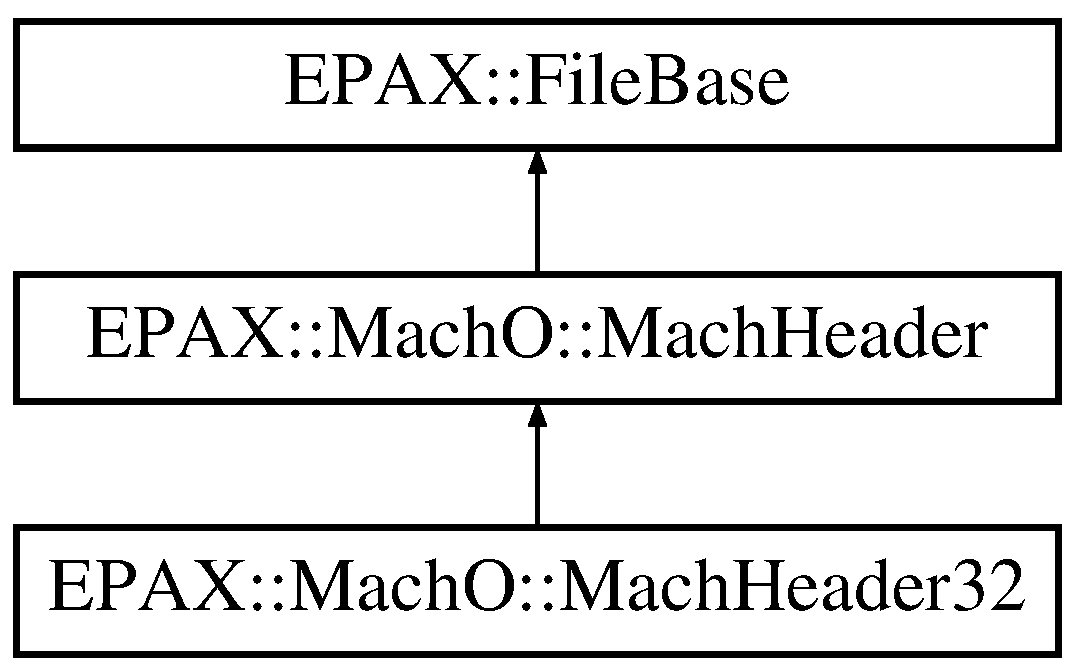
\includegraphics[height=3.000000cm]{class_e_p_a_x_1_1_mach_o_1_1_mach_header32}
\end{center}
\end{figure}
\subsection*{\-Public \-Member \-Functions}
\begin{DoxyCompactItemize}
\item 
\hyperlink{class_e_p_a_x_1_1_mach_o_1_1_mach_header32_a0878662183d5daaaca7398558c5aaf1b}{\-Mach\-Header32} (\hyperlink{class_e_p_a_x_1_1_base_binary}{\-Base\-Binary} $\ast$b, uint64\-\_\-t o)
\item 
virtual \hyperlink{class_e_p_a_x_1_1_mach_o_1_1_mach_header32_abf3abb3d4e236a8020adcaa9dfc840db}{$\sim$\-Mach\-Header32} ()
\item 
uint64\-\_\-t \hyperlink{class_e_p_a_x_1_1_mach_o_1_1_mach_header32_a4f0786ea334b1aae005caa3ea74231bb}{get\-Start\-Addr} ()
\item 
bool \hyperlink{class_e_p_a_x_1_1_mach_o_1_1_mach_header32_ab11fe95e26ef0b3f3eeabf4d9206d6b9}{verify} ()
\item 
bool \hyperlink{class_e_p_a_x_1_1_mach_o_1_1_mach_header32_a48f089963011dc2a1f04ca445445a29f}{is\-A\-R\-M} ()
\item 
void \hyperlink{class_e_p_a_x_1_1_mach_o_1_1_mach_header32_a4870b0179039c78eb507d2c63e818153}{describe} ()
\item 
uint32\-\_\-t \hyperlink{class_e_p_a_x_1_1_mach_o_1_1_mach_header32_a8b45baa84c71a8d1444d801df54c703e}{get\-File\-Type} ()
\end{DoxyCompactItemize}


\subsection{\-Detailed \-Description}


\-Definition at line 102 of file \-Mach\-O\-Binary.\-hpp.



\subsection{\-Constructor \& \-Destructor \-Documentation}
\hypertarget{class_e_p_a_x_1_1_mach_o_1_1_mach_header32_a0878662183d5daaaca7398558c5aaf1b}{\index{\-E\-P\-A\-X\-::\-Mach\-O\-::\-Mach\-Header32@{\-E\-P\-A\-X\-::\-Mach\-O\-::\-Mach\-Header32}!\-Mach\-Header32@{\-Mach\-Header32}}
\index{\-Mach\-Header32@{\-Mach\-Header32}!EPAX::MachO::MachHeader32@{\-E\-P\-A\-X\-::\-Mach\-O\-::\-Mach\-Header32}}
\subsubsection[{\-Mach\-Header32}]{\setlength{\rightskip}{0pt plus 5cm}{\bf \-E\-P\-A\-X\-::\-Mach\-O\-::\-Mach\-Header32\-::\-Mach\-Header32} (
\begin{DoxyParamCaption}
\item[{{\bf \-Base\-Binary} $\ast$}]{b, }
\item[{uint64\-\_\-t}]{o}
\end{DoxyParamCaption}
)}}\label{class_e_p_a_x_1_1_mach_o_1_1_mach_header32_a0878662183d5daaaca7398558c5aaf1b}


\-Definition at line 131 of file \-Mach\-O\-Binary.\-cpp.

\hypertarget{class_e_p_a_x_1_1_mach_o_1_1_mach_header32_abf3abb3d4e236a8020adcaa9dfc840db}{\index{\-E\-P\-A\-X\-::\-Mach\-O\-::\-Mach\-Header32@{\-E\-P\-A\-X\-::\-Mach\-O\-::\-Mach\-Header32}!$\sim$\-Mach\-Header32@{$\sim$\-Mach\-Header32}}
\index{$\sim$\-Mach\-Header32@{$\sim$\-Mach\-Header32}!EPAX::MachO::MachHeader32@{\-E\-P\-A\-X\-::\-Mach\-O\-::\-Mach\-Header32}}
\subsubsection[{$\sim$\-Mach\-Header32}]{\setlength{\rightskip}{0pt plus 5cm}virtual {\bf \-E\-P\-A\-X\-::\-Mach\-O\-::\-Mach\-Header32\-::$\sim$\-Mach\-Header32} (
\begin{DoxyParamCaption}
{}
\end{DoxyParamCaption}
)\hspace{0.3cm}{\ttfamily  \mbox{[}inline, virtual\mbox{]}}}}\label{class_e_p_a_x_1_1_mach_o_1_1_mach_header32_abf3abb3d4e236a8020adcaa9dfc840db}


\-Definition at line 106 of file \-Mach\-O\-Binary.\-hpp.



\subsection{\-Member \-Function \-Documentation}
\hypertarget{class_e_p_a_x_1_1_mach_o_1_1_mach_header32_a4870b0179039c78eb507d2c63e818153}{\index{\-E\-P\-A\-X\-::\-Mach\-O\-::\-Mach\-Header32@{\-E\-P\-A\-X\-::\-Mach\-O\-::\-Mach\-Header32}!describe@{describe}}
\index{describe@{describe}!EPAX::MachO::MachHeader32@{\-E\-P\-A\-X\-::\-Mach\-O\-::\-Mach\-Header32}}
\subsubsection[{describe}]{\setlength{\rightskip}{0pt plus 5cm}void {\bf \-E\-P\-A\-X\-::\-Mach\-O\-::\-Mach\-Header32\-::describe} (
\begin{DoxyParamCaption}
{}
\end{DoxyParamCaption}
)\hspace{0.3cm}{\ttfamily  \mbox{[}virtual\mbox{]}}}}\label{class_e_p_a_x_1_1_mach_o_1_1_mach_header32_a4870b0179039c78eb507d2c63e818153}


\-Implements \hyperlink{class_e_p_a_x_1_1_mach_o_1_1_mach_header_a6e04356c40b005cc7f9c8e318f327e2c}{\-E\-P\-A\-X\-::\-Mach\-O\-::\-Mach\-Header}.



\-Definition at line 228 of file \-Mach\-O\-Binary.\-cpp.

\hypertarget{class_e_p_a_x_1_1_mach_o_1_1_mach_header32_a8b45baa84c71a8d1444d801df54c703e}{\index{\-E\-P\-A\-X\-::\-Mach\-O\-::\-Mach\-Header32@{\-E\-P\-A\-X\-::\-Mach\-O\-::\-Mach\-Header32}!get\-File\-Type@{get\-File\-Type}}
\index{get\-File\-Type@{get\-File\-Type}!EPAX::MachO::MachHeader32@{\-E\-P\-A\-X\-::\-Mach\-O\-::\-Mach\-Header32}}
\subsubsection[{get\-File\-Type}]{\setlength{\rightskip}{0pt plus 5cm}uint32\-\_\-t {\bf \-E\-P\-A\-X\-::\-Mach\-O\-::\-Mach\-Header32\-::get\-File\-Type} (
\begin{DoxyParamCaption}
{}
\end{DoxyParamCaption}
)\hspace{0.3cm}{\ttfamily  \mbox{[}virtual\mbox{]}}}}\label{class_e_p_a_x_1_1_mach_o_1_1_mach_header32_a8b45baa84c71a8d1444d801df54c703e}


\-Implements \hyperlink{class_e_p_a_x_1_1_mach_o_1_1_mach_header_a667362bbcc5a18b89b430c3bbf9dbcf3}{\-E\-P\-A\-X\-::\-Mach\-O\-::\-Mach\-Header}.



\-Definition at line 178 of file \-Mach\-O\-Binary.\-cpp.

\hypertarget{class_e_p_a_x_1_1_mach_o_1_1_mach_header32_a4f0786ea334b1aae005caa3ea74231bb}{\index{\-E\-P\-A\-X\-::\-Mach\-O\-::\-Mach\-Header32@{\-E\-P\-A\-X\-::\-Mach\-O\-::\-Mach\-Header32}!get\-Start\-Addr@{get\-Start\-Addr}}
\index{get\-Start\-Addr@{get\-Start\-Addr}!EPAX::MachO::MachHeader32@{\-E\-P\-A\-X\-::\-Mach\-O\-::\-Mach\-Header32}}
\subsubsection[{get\-Start\-Addr}]{\setlength{\rightskip}{0pt plus 5cm}uint64\-\_\-t {\bf \-E\-P\-A\-X\-::\-Mach\-O\-::\-Mach\-Header32\-::get\-Start\-Addr} (
\begin{DoxyParamCaption}
{}
\end{DoxyParamCaption}
)\hspace{0.3cm}{\ttfamily  \mbox{[}virtual\mbox{]}}}}\label{class_e_p_a_x_1_1_mach_o_1_1_mach_header32_a4f0786ea334b1aae005caa3ea74231bb}


\-Implements \hyperlink{class_e_p_a_x_1_1_mach_o_1_1_mach_header_aeae22d677b30ceeed55c7f7910a45ff1}{\-E\-P\-A\-X\-::\-Mach\-O\-::\-Mach\-Header}.



\-Definition at line 145 of file \-Mach\-O\-Binary.\-cpp.

\hypertarget{class_e_p_a_x_1_1_mach_o_1_1_mach_header32_a48f089963011dc2a1f04ca445445a29f}{\index{\-E\-P\-A\-X\-::\-Mach\-O\-::\-Mach\-Header32@{\-E\-P\-A\-X\-::\-Mach\-O\-::\-Mach\-Header32}!is\-A\-R\-M@{is\-A\-R\-M}}
\index{is\-A\-R\-M@{is\-A\-R\-M}!EPAX::MachO::MachHeader32@{\-E\-P\-A\-X\-::\-Mach\-O\-::\-Mach\-Header32}}
\subsubsection[{is\-A\-R\-M}]{\setlength{\rightskip}{0pt plus 5cm}bool {\bf \-E\-P\-A\-X\-::\-Mach\-O\-::\-Mach\-Header32\-::is\-A\-R\-M} (
\begin{DoxyParamCaption}
{}
\end{DoxyParamCaption}
)\hspace{0.3cm}{\ttfamily  \mbox{[}virtual\mbox{]}}}}\label{class_e_p_a_x_1_1_mach_o_1_1_mach_header32_a48f089963011dc2a1f04ca445445a29f}


\-Implements \hyperlink{class_e_p_a_x_1_1_mach_o_1_1_mach_header_a95466e1612d0ad48d991830f4c3898ee}{\-E\-P\-A\-X\-::\-Mach\-O\-::\-Mach\-Header}.



\-Definition at line 167 of file \-Mach\-O\-Binary.\-cpp.

\hypertarget{class_e_p_a_x_1_1_mach_o_1_1_mach_header32_ab11fe95e26ef0b3f3eeabf4d9206d6b9}{\index{\-E\-P\-A\-X\-::\-Mach\-O\-::\-Mach\-Header32@{\-E\-P\-A\-X\-::\-Mach\-O\-::\-Mach\-Header32}!verify@{verify}}
\index{verify@{verify}!EPAX::MachO::MachHeader32@{\-E\-P\-A\-X\-::\-Mach\-O\-::\-Mach\-Header32}}
\subsubsection[{verify}]{\setlength{\rightskip}{0pt plus 5cm}bool {\bf \-E\-P\-A\-X\-::\-Mach\-O\-::\-Mach\-Header32\-::verify} (
\begin{DoxyParamCaption}
{}
\end{DoxyParamCaption}
)\hspace{0.3cm}{\ttfamily  \mbox{[}virtual\mbox{]}}}}\label{class_e_p_a_x_1_1_mach_o_1_1_mach_header32_ab11fe95e26ef0b3f3eeabf4d9206d6b9}


\-Implements \hyperlink{class_e_p_a_x_1_1_mach_o_1_1_mach_header_aeca0eb4432fece14fc5bb27810a63e06}{\-E\-P\-A\-X\-::\-Mach\-O\-::\-Mach\-Header}.



\-Definition at line 153 of file \-Mach\-O\-Binary.\-cpp.



\-The documentation for this class was generated from the following files\-:\begin{DoxyCompactItemize}
\item 
\hyperlink{_mach_o_binary_8hpp}{\-Mach\-O\-Binary.\-hpp}\item 
\hyperlink{_mach_o_binary_8cpp}{\-Mach\-O\-Binary.\-cpp}\end{DoxyCompactItemize}

\hypertarget{class_e_p_a_x_1_1_mach_o_1_1_mach_header64}{\section{\-E\-P\-A\-X\-:\-:\-Mach\-O\-:\-:\-Mach\-Header64 \-Class \-Reference}
\label{class_e_p_a_x_1_1_mach_o_1_1_mach_header64}\index{\-E\-P\-A\-X\-::\-Mach\-O\-::\-Mach\-Header64@{\-E\-P\-A\-X\-::\-Mach\-O\-::\-Mach\-Header64}}
}


{\ttfamily \#include $<$\-Mach\-O\-Binary.\-hpp$>$}

\-Inheritance diagram for \-E\-P\-A\-X\-:\-:\-Mach\-O\-:\-:\-Mach\-Header64\-:\begin{figure}[H]
\begin{center}
\leavevmode
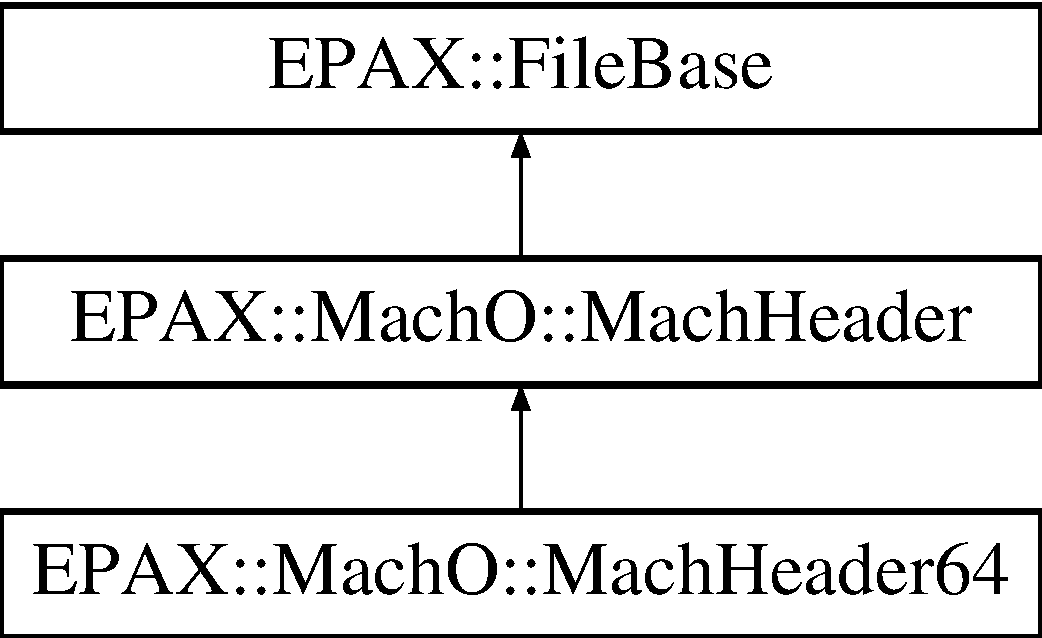
\includegraphics[height=3.000000cm]{class_e_p_a_x_1_1_mach_o_1_1_mach_header64}
\end{center}
\end{figure}
\subsection*{\-Public \-Member \-Functions}
\begin{DoxyCompactItemize}
\item 
\hyperlink{class_e_p_a_x_1_1_mach_o_1_1_mach_header64_ac5d9773a0ff71021b6b77e014b1c8bfd}{\-Mach\-Header64} (\hyperlink{class_e_p_a_x_1_1_base_binary}{\-Base\-Binary} $\ast$b, uint64\-\_\-t o)
\item 
virtual \hyperlink{class_e_p_a_x_1_1_mach_o_1_1_mach_header64_aa4f1dff7a22f261611849b2135fac9a3}{$\sim$\-Mach\-Header64} ()
\item 
uint64\-\_\-t \hyperlink{class_e_p_a_x_1_1_mach_o_1_1_mach_header64_a836f1c7e06d79c858b68f80a66741f36}{get\-Start\-Addr} ()
\item 
bool \hyperlink{class_e_p_a_x_1_1_mach_o_1_1_mach_header64_a6adb13e5a45f8fde528dcfea1c8ae0dd}{verify} ()
\item 
bool \hyperlink{class_e_p_a_x_1_1_mach_o_1_1_mach_header64_a8046b0bfdf50acbf3e161b317d475516}{is\-A\-R\-M} ()
\item 
void \hyperlink{class_e_p_a_x_1_1_mach_o_1_1_mach_header64_ad56f5abdcfd8bf2898d5e2cf72ad045d}{describe} ()
\item 
uint32\-\_\-t \hyperlink{class_e_p_a_x_1_1_mach_o_1_1_mach_header64_a3dd521883885b8ccc0d7731b90ba873d}{get\-File\-Type} ()
\end{DoxyCompactItemize}


\subsection{\-Detailed \-Description}


\-Definition at line 115 of file \-Mach\-O\-Binary.\-hpp.



\subsection{\-Constructor \& \-Destructor \-Documentation}
\hypertarget{class_e_p_a_x_1_1_mach_o_1_1_mach_header64_ac5d9773a0ff71021b6b77e014b1c8bfd}{\index{\-E\-P\-A\-X\-::\-Mach\-O\-::\-Mach\-Header64@{\-E\-P\-A\-X\-::\-Mach\-O\-::\-Mach\-Header64}!\-Mach\-Header64@{\-Mach\-Header64}}
\index{\-Mach\-Header64@{\-Mach\-Header64}!EPAX::MachO::MachHeader64@{\-E\-P\-A\-X\-::\-Mach\-O\-::\-Mach\-Header64}}
\subsubsection[{\-Mach\-Header64}]{\setlength{\rightskip}{0pt plus 5cm}{\bf \-E\-P\-A\-X\-::\-Mach\-O\-::\-Mach\-Header64\-::\-Mach\-Header64} (
\begin{DoxyParamCaption}
\item[{{\bf \-Base\-Binary} $\ast$}]{b, }
\item[{uint64\-\_\-t}]{o}
\end{DoxyParamCaption}
)}}\label{class_e_p_a_x_1_1_mach_o_1_1_mach_header64_ac5d9773a0ff71021b6b77e014b1c8bfd}


\-Definition at line 138 of file \-Mach\-O\-Binary.\-cpp.

\hypertarget{class_e_p_a_x_1_1_mach_o_1_1_mach_header64_aa4f1dff7a22f261611849b2135fac9a3}{\index{\-E\-P\-A\-X\-::\-Mach\-O\-::\-Mach\-Header64@{\-E\-P\-A\-X\-::\-Mach\-O\-::\-Mach\-Header64}!$\sim$\-Mach\-Header64@{$\sim$\-Mach\-Header64}}
\index{$\sim$\-Mach\-Header64@{$\sim$\-Mach\-Header64}!EPAX::MachO::MachHeader64@{\-E\-P\-A\-X\-::\-Mach\-O\-::\-Mach\-Header64}}
\subsubsection[{$\sim$\-Mach\-Header64}]{\setlength{\rightskip}{0pt plus 5cm}virtual {\bf \-E\-P\-A\-X\-::\-Mach\-O\-::\-Mach\-Header64\-::$\sim$\-Mach\-Header64} (
\begin{DoxyParamCaption}
{}
\end{DoxyParamCaption}
)\hspace{0.3cm}{\ttfamily  \mbox{[}inline, virtual\mbox{]}}}}\label{class_e_p_a_x_1_1_mach_o_1_1_mach_header64_aa4f1dff7a22f261611849b2135fac9a3}


\-Definition at line 118 of file \-Mach\-O\-Binary.\-hpp.



\subsection{\-Member \-Function \-Documentation}
\hypertarget{class_e_p_a_x_1_1_mach_o_1_1_mach_header64_ad56f5abdcfd8bf2898d5e2cf72ad045d}{\index{\-E\-P\-A\-X\-::\-Mach\-O\-::\-Mach\-Header64@{\-E\-P\-A\-X\-::\-Mach\-O\-::\-Mach\-Header64}!describe@{describe}}
\index{describe@{describe}!EPAX::MachO::MachHeader64@{\-E\-P\-A\-X\-::\-Mach\-O\-::\-Mach\-Header64}}
\subsubsection[{describe}]{\setlength{\rightskip}{0pt plus 5cm}void {\bf \-E\-P\-A\-X\-::\-Mach\-O\-::\-Mach\-Header64\-::describe} (
\begin{DoxyParamCaption}
{}
\end{DoxyParamCaption}
)\hspace{0.3cm}{\ttfamily  \mbox{[}virtual\mbox{]}}}}\label{class_e_p_a_x_1_1_mach_o_1_1_mach_header64_ad56f5abdcfd8bf2898d5e2cf72ad045d}


\-Implements \hyperlink{class_e_p_a_x_1_1_mach_o_1_1_mach_header_a6e04356c40b005cc7f9c8e318f327e2c}{\-E\-P\-A\-X\-::\-Mach\-O\-::\-Mach\-Header}.



\-Definition at line 234 of file \-Mach\-O\-Binary.\-cpp.

\hypertarget{class_e_p_a_x_1_1_mach_o_1_1_mach_header64_a3dd521883885b8ccc0d7731b90ba873d}{\index{\-E\-P\-A\-X\-::\-Mach\-O\-::\-Mach\-Header64@{\-E\-P\-A\-X\-::\-Mach\-O\-::\-Mach\-Header64}!get\-File\-Type@{get\-File\-Type}}
\index{get\-File\-Type@{get\-File\-Type}!EPAX::MachO::MachHeader64@{\-E\-P\-A\-X\-::\-Mach\-O\-::\-Mach\-Header64}}
\subsubsection[{get\-File\-Type}]{\setlength{\rightskip}{0pt plus 5cm}uint32\-\_\-t {\bf \-E\-P\-A\-X\-::\-Mach\-O\-::\-Mach\-Header64\-::get\-File\-Type} (
\begin{DoxyParamCaption}
{}
\end{DoxyParamCaption}
)\hspace{0.3cm}{\ttfamily  \mbox{[}virtual\mbox{]}}}}\label{class_e_p_a_x_1_1_mach_o_1_1_mach_header64_a3dd521883885b8ccc0d7731b90ba873d}


\-Implements \hyperlink{class_e_p_a_x_1_1_mach_o_1_1_mach_header_a667362bbcc5a18b89b430c3bbf9dbcf3}{\-E\-P\-A\-X\-::\-Mach\-O\-::\-Mach\-Header}.



\-Definition at line 182 of file \-Mach\-O\-Binary.\-cpp.

\hypertarget{class_e_p_a_x_1_1_mach_o_1_1_mach_header64_a836f1c7e06d79c858b68f80a66741f36}{\index{\-E\-P\-A\-X\-::\-Mach\-O\-::\-Mach\-Header64@{\-E\-P\-A\-X\-::\-Mach\-O\-::\-Mach\-Header64}!get\-Start\-Addr@{get\-Start\-Addr}}
\index{get\-Start\-Addr@{get\-Start\-Addr}!EPAX::MachO::MachHeader64@{\-E\-P\-A\-X\-::\-Mach\-O\-::\-Mach\-Header64}}
\subsubsection[{get\-Start\-Addr}]{\setlength{\rightskip}{0pt plus 5cm}uint64\-\_\-t {\bf \-E\-P\-A\-X\-::\-Mach\-O\-::\-Mach\-Header64\-::get\-Start\-Addr} (
\begin{DoxyParamCaption}
{}
\end{DoxyParamCaption}
)\hspace{0.3cm}{\ttfamily  \mbox{[}virtual\mbox{]}}}}\label{class_e_p_a_x_1_1_mach_o_1_1_mach_header64_a836f1c7e06d79c858b68f80a66741f36}


\-Implements \hyperlink{class_e_p_a_x_1_1_mach_o_1_1_mach_header_aeae22d677b30ceeed55c7f7910a45ff1}{\-E\-P\-A\-X\-::\-Mach\-O\-::\-Mach\-Header}.



\-Definition at line 149 of file \-Mach\-O\-Binary.\-cpp.

\hypertarget{class_e_p_a_x_1_1_mach_o_1_1_mach_header64_a8046b0bfdf50acbf3e161b317d475516}{\index{\-E\-P\-A\-X\-::\-Mach\-O\-::\-Mach\-Header64@{\-E\-P\-A\-X\-::\-Mach\-O\-::\-Mach\-Header64}!is\-A\-R\-M@{is\-A\-R\-M}}
\index{is\-A\-R\-M@{is\-A\-R\-M}!EPAX::MachO::MachHeader64@{\-E\-P\-A\-X\-::\-Mach\-O\-::\-Mach\-Header64}}
\subsubsection[{is\-A\-R\-M}]{\setlength{\rightskip}{0pt plus 5cm}bool {\bf \-E\-P\-A\-X\-::\-Mach\-O\-::\-Mach\-Header64\-::is\-A\-R\-M} (
\begin{DoxyParamCaption}
{}
\end{DoxyParamCaption}
)\hspace{0.3cm}{\ttfamily  \mbox{[}virtual\mbox{]}}}}\label{class_e_p_a_x_1_1_mach_o_1_1_mach_header64_a8046b0bfdf50acbf3e161b317d475516}


\-Implements \hyperlink{class_e_p_a_x_1_1_mach_o_1_1_mach_header_a95466e1612d0ad48d991830f4c3898ee}{\-E\-P\-A\-X\-::\-Mach\-O\-::\-Mach\-Header}.



\-Definition at line 173 of file \-Mach\-O\-Binary.\-cpp.

\hypertarget{class_e_p_a_x_1_1_mach_o_1_1_mach_header64_a6adb13e5a45f8fde528dcfea1c8ae0dd}{\index{\-E\-P\-A\-X\-::\-Mach\-O\-::\-Mach\-Header64@{\-E\-P\-A\-X\-::\-Mach\-O\-::\-Mach\-Header64}!verify@{verify}}
\index{verify@{verify}!EPAX::MachO::MachHeader64@{\-E\-P\-A\-X\-::\-Mach\-O\-::\-Mach\-Header64}}
\subsubsection[{verify}]{\setlength{\rightskip}{0pt plus 5cm}bool {\bf \-E\-P\-A\-X\-::\-Mach\-O\-::\-Mach\-Header64\-::verify} (
\begin{DoxyParamCaption}
{}
\end{DoxyParamCaption}
)\hspace{0.3cm}{\ttfamily  \mbox{[}virtual\mbox{]}}}}\label{class_e_p_a_x_1_1_mach_o_1_1_mach_header64_a6adb13e5a45f8fde528dcfea1c8ae0dd}


\-Implements \hyperlink{class_e_p_a_x_1_1_mach_o_1_1_mach_header_aeca0eb4432fece14fc5bb27810a63e06}{\-E\-P\-A\-X\-::\-Mach\-O\-::\-Mach\-Header}.



\-Definition at line 160 of file \-Mach\-O\-Binary.\-cpp.



\-The documentation for this class was generated from the following files\-:\begin{DoxyCompactItemize}
\item 
\hyperlink{_mach_o_binary_8hpp}{\-Mach\-O\-Binary.\-hpp}\item 
\hyperlink{_mach_o_binary_8cpp}{\-Mach\-O\-Binary.\-cpp}\end{DoxyCompactItemize}

\hypertarget{class_e_p_a_x_1_1_mach_o_1_1_mach_o_binary}{\section{\-E\-P\-A\-X\-:\-:\-Mach\-O\-:\-:\-Mach\-O\-Binary \-Class \-Reference}
\label{class_e_p_a_x_1_1_mach_o_1_1_mach_o_binary}\index{\-E\-P\-A\-X\-::\-Mach\-O\-::\-Mach\-O\-Binary@{\-E\-P\-A\-X\-::\-Mach\-O\-::\-Mach\-O\-Binary}}
}


{\ttfamily \#include $<$\-Mach\-O\-Binary.\-hpp$>$}

\-Inheritance diagram for \-E\-P\-A\-X\-:\-:\-Mach\-O\-:\-:\-Mach\-O\-Binary\-:\begin{figure}[H]
\begin{center}
\leavevmode
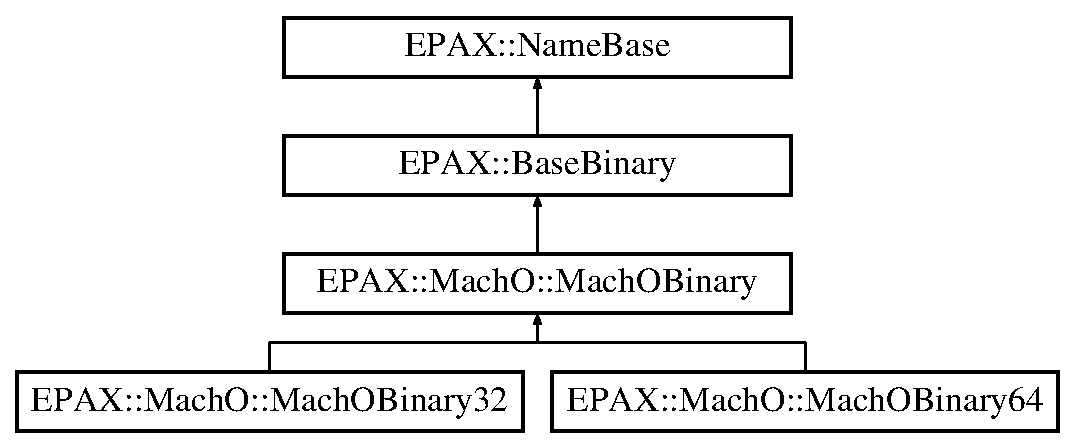
\includegraphics[height=4.000000cm]{class_e_p_a_x_1_1_mach_o_1_1_mach_o_binary}
\end{center}
\end{figure}
\subsection*{\-Public \-Member \-Functions}
\begin{DoxyCompactItemize}
\item 
\hyperlink{class_e_p_a_x_1_1_mach_o_1_1_mach_o_binary_a753d91d032788ea99e964c5f7b59a003}{\-Mach\-O\-Binary} (std\-::string n)
\item 
virtual \hyperlink{class_e_p_a_x_1_1_mach_o_1_1_mach_o_binary_a5a255df5d7799f13411d3ecb2dda045d}{$\sim$\-Mach\-O\-Binary} ()
\item 
virtual \hyperlink{namespace_e_p_a_x_a4be639c006ef14def4708b37ee6dd67d}{\-Binary\-Format} \hyperlink{class_e_p_a_x_1_1_mach_o_1_1_mach_o_binary_a435106c1f40d1ec16ac539fbdecd88bd}{get\-Format} ()=0
\item 
uint64\-\_\-t \hyperlink{class_e_p_a_x_1_1_mach_o_1_1_mach_o_binary_a426e6fdd744908571c46e10608211df4}{get\-Start\-Addr} ()
\item 
void \hyperlink{class_e_p_a_x_1_1_mach_o_1_1_mach_o_binary_a3a4b9b3138d22d2455fbddb4c694f532}{emit} (std\-::string n)
\item 
bool \hyperlink{class_e_p_a_x_1_1_mach_o_1_1_mach_o_binary_aa0eb9a16309170238ca0d3cc027a116b}{verify} ()
\item 
bool \hyperlink{class_e_p_a_x_1_1_mach_o_1_1_mach_o_binary_a7d857ef9a99dc9d553e7e764234db957}{is\-A\-R\-M} ()
\item 
void \hyperlink{class_e_p_a_x_1_1_mach_o_1_1_mach_o_binary_a7142994ba41ef1a5fad2d34e75278764}{describe} ()
\item 
bool \hyperlink{class_e_p_a_x_1_1_mach_o_1_1_mach_o_binary_a6c3c547d72fe13a51b702fcfc6c1c271}{is32\-Bit} ()
\item 
bool \hyperlink{class_e_p_a_x_1_1_mach_o_1_1_mach_o_binary_a892a753783fa1feaa3f98fcad476da8a}{is64\-Bit} ()
\item 
bool \hyperlink{class_e_p_a_x_1_1_mach_o_1_1_mach_o_binary_a6031c2f4420ec57b008d33a27f490a51}{is\-Executable} ()
\item 
void \hyperlink{class_e_p_a_x_1_1_mach_o_1_1_mach_o_binary_a06e7ed071e394bd70b2a371b1360f591}{find\-Functions} ()
\item 
void \hyperlink{class_e_p_a_x_1_1_mach_o_1_1_mach_o_binary_a4c92ec8fe5a4c63d57b101f1e35f9291}{find\-Symbols} ()
\item 
void \hyperlink{class_e_p_a_x_1_1_mach_o_1_1_mach_o_binary_a91a0d99f8a2bf0ff9c6a0870eaf232cb}{find\-Sections} ()
\item 
bool \hyperlink{class_e_p_a_x_1_1_mach_o_1_1_mach_o_binary_a37bd8cd22a68dc0fe4836c5781568725}{inside\-Text\-Range} (uint64\-\_\-t a)
\item 
uint64\-\_\-t \hyperlink{class_e_p_a_x_1_1_mach_o_1_1_mach_o_binary_a5b58a3105ffe8aff09dc2c20421e8744}{function\-End\-Address} (\hyperlink{class_e_p_a_x_1_1_function}{\-Function} $\ast$f, \hyperlink{class_e_p_a_x_1_1_function}{\-Function} $\ast$nextf)
\item 
void \hyperlink{class_e_p_a_x_1_1_mach_o_1_1_mach_o_binary_a654a69dcd9a459f5e78b740047b94fa0}{print\-Sections} (std\-::ostream \&stream=std\-::cout)
\item 
void \hyperlink{class_e_p_a_x_1_1_mach_o_1_1_mach_o_binary_ad6b3af54bfd54fa0f37f22efc94fc985}{print\-Functions} (std\-::ostream \&stream=std\-::cout)
\end{DoxyCompactItemize}
\subsection*{\-Protected \-Attributes}
\begin{DoxyCompactItemize}
\item 
\hyperlink{class_e_p_a_x_1_1_mach_o_1_1_mach_header}{\-Mach\-Header} $\ast$ \hyperlink{class_e_p_a_x_1_1_mach_o_1_1_mach_o_binary_a3ce1fa66447d472ddf807a42777cd099}{machheader}
\end{DoxyCompactItemize}


\subsection{\-Detailed \-Description}


\-Definition at line 37 of file \-Mach\-O\-Binary.\-hpp.



\subsection{\-Constructor \& \-Destructor \-Documentation}
\hypertarget{class_e_p_a_x_1_1_mach_o_1_1_mach_o_binary_a753d91d032788ea99e964c5f7b59a003}{\index{\-E\-P\-A\-X\-::\-Mach\-O\-::\-Mach\-O\-Binary@{\-E\-P\-A\-X\-::\-Mach\-O\-::\-Mach\-O\-Binary}!\-Mach\-O\-Binary@{\-Mach\-O\-Binary}}
\index{\-Mach\-O\-Binary@{\-Mach\-O\-Binary}!EPAX::MachO::MachOBinary@{\-E\-P\-A\-X\-::\-Mach\-O\-::\-Mach\-O\-Binary}}
\subsubsection[{\-Mach\-O\-Binary}]{\setlength{\rightskip}{0pt plus 5cm}{\bf \-E\-P\-A\-X\-::\-Mach\-O\-::\-Mach\-O\-Binary\-::\-Mach\-O\-Binary} (
\begin{DoxyParamCaption}
\item[{std\-::string}]{n}
\end{DoxyParamCaption}
)}}\label{class_e_p_a_x_1_1_mach_o_1_1_mach_o_binary_a753d91d032788ea99e964c5f7b59a003}


\-Definition at line 40 of file \-Mach\-O\-Binary.\-cpp.

\hypertarget{class_e_p_a_x_1_1_mach_o_1_1_mach_o_binary_a5a255df5d7799f13411d3ecb2dda045d}{\index{\-E\-P\-A\-X\-::\-Mach\-O\-::\-Mach\-O\-Binary@{\-E\-P\-A\-X\-::\-Mach\-O\-::\-Mach\-O\-Binary}!$\sim$\-Mach\-O\-Binary@{$\sim$\-Mach\-O\-Binary}}
\index{$\sim$\-Mach\-O\-Binary@{$\sim$\-Mach\-O\-Binary}!EPAX::MachO::MachOBinary@{\-E\-P\-A\-X\-::\-Mach\-O\-::\-Mach\-O\-Binary}}
\subsubsection[{$\sim$\-Mach\-O\-Binary}]{\setlength{\rightskip}{0pt plus 5cm}{\bf \-E\-P\-A\-X\-::\-Mach\-O\-::\-Mach\-O\-Binary\-::$\sim$\-Mach\-O\-Binary} (
\begin{DoxyParamCaption}
{}
\end{DoxyParamCaption}
)\hspace{0.3cm}{\ttfamily  \mbox{[}virtual\mbox{]}}}}\label{class_e_p_a_x_1_1_mach_o_1_1_mach_o_binary_a5a255df5d7799f13411d3ecb2dda045d}


\-Definition at line 45 of file \-Mach\-O\-Binary.\-cpp.



\subsection{\-Member \-Function \-Documentation}
\hypertarget{class_e_p_a_x_1_1_mach_o_1_1_mach_o_binary_a7142994ba41ef1a5fad2d34e75278764}{\index{\-E\-P\-A\-X\-::\-Mach\-O\-::\-Mach\-O\-Binary@{\-E\-P\-A\-X\-::\-Mach\-O\-::\-Mach\-O\-Binary}!describe@{describe}}
\index{describe@{describe}!EPAX::MachO::MachOBinary@{\-E\-P\-A\-X\-::\-Mach\-O\-::\-Mach\-O\-Binary}}
\subsubsection[{describe}]{\setlength{\rightskip}{0pt plus 5cm}void {\bf \-E\-P\-A\-X\-::\-Mach\-O\-::\-Mach\-O\-Binary\-::describe} (
\begin{DoxyParamCaption}
{}
\end{DoxyParamCaption}
)\hspace{0.3cm}{\ttfamily  \mbox{[}virtual\mbox{]}}}}\label{class_e_p_a_x_1_1_mach_o_1_1_mach_o_binary_a7142994ba41ef1a5fad2d34e75278764}


\-Implements \hyperlink{class_e_p_a_x_1_1_base_binary_a501175cac7fb1650bf378d6b4729c1ec}{\-E\-P\-A\-X\-::\-Base\-Binary}.



\-Definition at line 95 of file \-Mach\-O\-Binary.\-cpp.

\hypertarget{class_e_p_a_x_1_1_mach_o_1_1_mach_o_binary_a3a4b9b3138d22d2455fbddb4c694f532}{\index{\-E\-P\-A\-X\-::\-Mach\-O\-::\-Mach\-O\-Binary@{\-E\-P\-A\-X\-::\-Mach\-O\-::\-Mach\-O\-Binary}!emit@{emit}}
\index{emit@{emit}!EPAX::MachO::MachOBinary@{\-E\-P\-A\-X\-::\-Mach\-O\-::\-Mach\-O\-Binary}}
\subsubsection[{emit}]{\setlength{\rightskip}{0pt plus 5cm}void {\bf \-E\-P\-A\-X\-::\-Mach\-O\-::\-Mach\-O\-Binary\-::emit} (
\begin{DoxyParamCaption}
\item[{std\-::string}]{n}
\end{DoxyParamCaption}
)\hspace{0.3cm}{\ttfamily  \mbox{[}virtual\mbox{]}}}}\label{class_e_p_a_x_1_1_mach_o_1_1_mach_o_binary_a3a4b9b3138d22d2455fbddb4c694f532}


\-Implements \hyperlink{class_e_p_a_x_1_1_base_binary_a8883d3b0580cae0f5a1960c6fbfd6a1f}{\-E\-P\-A\-X\-::\-Base\-Binary}.



\-Definition at line 83 of file \-Mach\-O\-Binary.\-cpp.

\hypertarget{class_e_p_a_x_1_1_mach_o_1_1_mach_o_binary_a06e7ed071e394bd70b2a371b1360f591}{\index{\-E\-P\-A\-X\-::\-Mach\-O\-::\-Mach\-O\-Binary@{\-E\-P\-A\-X\-::\-Mach\-O\-::\-Mach\-O\-Binary}!find\-Functions@{find\-Functions}}
\index{find\-Functions@{find\-Functions}!EPAX::MachO::MachOBinary@{\-E\-P\-A\-X\-::\-Mach\-O\-::\-Mach\-O\-Binary}}
\subsubsection[{find\-Functions}]{\setlength{\rightskip}{0pt plus 5cm}void {\bf \-E\-P\-A\-X\-::\-Mach\-O\-::\-Mach\-O\-Binary\-::find\-Functions} (
\begin{DoxyParamCaption}
{}
\end{DoxyParamCaption}
)\hspace{0.3cm}{\ttfamily  \mbox{[}virtual\mbox{]}}}}\label{class_e_p_a_x_1_1_mach_o_1_1_mach_o_binary_a06e7ed071e394bd70b2a371b1360f591}
\-Finds and internally stores all functions in the image

\begin{DoxyReturn}{\-Returns}
none 
\end{DoxyReturn}


\-Implements \hyperlink{class_e_p_a_x_1_1_base_binary_abcd76218158ab20a2f81d68a537b21cb}{\-E\-P\-A\-X\-::\-Base\-Binary}.



\-Definition at line 99 of file \-Mach\-O\-Binary.\-cpp.

\hypertarget{class_e_p_a_x_1_1_mach_o_1_1_mach_o_binary_a91a0d99f8a2bf0ff9c6a0870eaf232cb}{\index{\-E\-P\-A\-X\-::\-Mach\-O\-::\-Mach\-O\-Binary@{\-E\-P\-A\-X\-::\-Mach\-O\-::\-Mach\-O\-Binary}!find\-Sections@{find\-Sections}}
\index{find\-Sections@{find\-Sections}!EPAX::MachO::MachOBinary@{\-E\-P\-A\-X\-::\-Mach\-O\-::\-Mach\-O\-Binary}}
\subsubsection[{find\-Sections}]{\setlength{\rightskip}{0pt plus 5cm}void {\bf \-E\-P\-A\-X\-::\-Mach\-O\-::\-Mach\-O\-Binary\-::find\-Sections} (
\begin{DoxyParamCaption}
{}
\end{DoxyParamCaption}
)}}\label{class_e_p_a_x_1_1_mach_o_1_1_mach_o_binary_a91a0d99f8a2bf0ff9c6a0870eaf232cb}


\-Definition at line 107 of file \-Mach\-O\-Binary.\-cpp.

\hypertarget{class_e_p_a_x_1_1_mach_o_1_1_mach_o_binary_a4c92ec8fe5a4c63d57b101f1e35f9291}{\index{\-E\-P\-A\-X\-::\-Mach\-O\-::\-Mach\-O\-Binary@{\-E\-P\-A\-X\-::\-Mach\-O\-::\-Mach\-O\-Binary}!find\-Symbols@{find\-Symbols}}
\index{find\-Symbols@{find\-Symbols}!EPAX::MachO::MachOBinary@{\-E\-P\-A\-X\-::\-Mach\-O\-::\-Mach\-O\-Binary}}
\subsubsection[{find\-Symbols}]{\setlength{\rightskip}{0pt plus 5cm}void {\bf \-E\-P\-A\-X\-::\-Mach\-O\-::\-Mach\-O\-Binary\-::find\-Symbols} (
\begin{DoxyParamCaption}
{}
\end{DoxyParamCaption}
)\hspace{0.3cm}{\ttfamily  \mbox{[}virtual\mbox{]}}}}\label{class_e_p_a_x_1_1_mach_o_1_1_mach_o_binary_a4c92ec8fe5a4c63d57b101f1e35f9291}
\-Finds and internally stores all symbols in the image

\begin{DoxyReturn}{\-Returns}
none 
\end{DoxyReturn}


\-Implements \hyperlink{class_e_p_a_x_1_1_base_binary_adc22abd64f6a873fbce30c79508322fe}{\-E\-P\-A\-X\-::\-Base\-Binary}.



\-Definition at line 103 of file \-Mach\-O\-Binary.\-cpp.

\hypertarget{class_e_p_a_x_1_1_mach_o_1_1_mach_o_binary_a5b58a3105ffe8aff09dc2c20421e8744}{\index{\-E\-P\-A\-X\-::\-Mach\-O\-::\-Mach\-O\-Binary@{\-E\-P\-A\-X\-::\-Mach\-O\-::\-Mach\-O\-Binary}!function\-End\-Address@{function\-End\-Address}}
\index{function\-End\-Address@{function\-End\-Address}!EPAX::MachO::MachOBinary@{\-E\-P\-A\-X\-::\-Mach\-O\-::\-Mach\-O\-Binary}}
\subsubsection[{function\-End\-Address}]{\setlength{\rightskip}{0pt plus 5cm}uint64\-\_\-t {\bf \-E\-P\-A\-X\-::\-Mach\-O\-::\-Mach\-O\-Binary\-::function\-End\-Address} (
\begin{DoxyParamCaption}
\item[{{\bf \-Function} $\ast$}]{f, }
\item[{{\bf \-Function} $\ast$}]{nextf}
\end{DoxyParamCaption}
)\hspace{0.3cm}{\ttfamily  \mbox{[}virtual\mbox{]}}}}\label{class_e_p_a_x_1_1_mach_o_1_1_mach_o_binary_a5b58a3105ffe8aff09dc2c20421e8744}


\-Implements \hyperlink{class_e_p_a_x_1_1_base_binary_a3ebaa616622aaca98685ece5d59c05d8}{\-E\-P\-A\-X\-::\-Base\-Binary}.



\-Definition at line 51 of file \-Mach\-O\-Binary.\-cpp.

\hypertarget{class_e_p_a_x_1_1_mach_o_1_1_mach_o_binary_a435106c1f40d1ec16ac539fbdecd88bd}{\index{\-E\-P\-A\-X\-::\-Mach\-O\-::\-Mach\-O\-Binary@{\-E\-P\-A\-X\-::\-Mach\-O\-::\-Mach\-O\-Binary}!get\-Format@{get\-Format}}
\index{get\-Format@{get\-Format}!EPAX::MachO::MachOBinary@{\-E\-P\-A\-X\-::\-Mach\-O\-::\-Mach\-O\-Binary}}
\subsubsection[{get\-Format}]{\setlength{\rightskip}{0pt plus 5cm}virtual {\bf \-Binary\-Format} {\bf \-E\-P\-A\-X\-::\-Mach\-O\-::\-Mach\-O\-Binary\-::get\-Format} (
\begin{DoxyParamCaption}
{}
\end{DoxyParamCaption}
)\hspace{0.3cm}{\ttfamily  \mbox{[}pure virtual\mbox{]}}}}\label{class_e_p_a_x_1_1_mach_o_1_1_mach_o_binary_a435106c1f40d1ec16ac539fbdecd88bd}


\-Implements \hyperlink{class_e_p_a_x_1_1_base_binary_a456741cd16605e5035ab89ab813f4373}{\-E\-P\-A\-X\-::\-Base\-Binary}.



\-Implemented in \hyperlink{class_e_p_a_x_1_1_mach_o_1_1_mach_o_binary64_ab2aa03d22ba0339c415a9dc9e6a0912b}{\-E\-P\-A\-X\-::\-Mach\-O\-::\-Mach\-O\-Binary64}, and \hyperlink{class_e_p_a_x_1_1_mach_o_1_1_mach_o_binary32_a37eab3a09ee0f670f2633a56c890100e}{\-E\-P\-A\-X\-::\-Mach\-O\-::\-Mach\-O\-Binary32}.

\hypertarget{class_e_p_a_x_1_1_mach_o_1_1_mach_o_binary_a426e6fdd744908571c46e10608211df4}{\index{\-E\-P\-A\-X\-::\-Mach\-O\-::\-Mach\-O\-Binary@{\-E\-P\-A\-X\-::\-Mach\-O\-::\-Mach\-O\-Binary}!get\-Start\-Addr@{get\-Start\-Addr}}
\index{get\-Start\-Addr@{get\-Start\-Addr}!EPAX::MachO::MachOBinary@{\-E\-P\-A\-X\-::\-Mach\-O\-::\-Mach\-O\-Binary}}
\subsubsection[{get\-Start\-Addr}]{\setlength{\rightskip}{0pt plus 5cm}uint64\-\_\-t {\bf \-E\-P\-A\-X\-::\-Mach\-O\-::\-Mach\-O\-Binary\-::get\-Start\-Addr} (
\begin{DoxyParamCaption}
{}
\end{DoxyParamCaption}
)\hspace{0.3cm}{\ttfamily  \mbox{[}virtual\mbox{]}}}}\label{class_e_p_a_x_1_1_mach_o_1_1_mach_o_binary_a426e6fdd744908571c46e10608211df4}


\-Implements \hyperlink{class_e_p_a_x_1_1_base_binary_ad23fe3f3a6f5b387df2f4eb7e4a4f23d}{\-E\-P\-A\-X\-::\-Base\-Binary}.



\-Definition at line 67 of file \-Mach\-O\-Binary.\-cpp.

\hypertarget{class_e_p_a_x_1_1_mach_o_1_1_mach_o_binary_a37bd8cd22a68dc0fe4836c5781568725}{\index{\-E\-P\-A\-X\-::\-Mach\-O\-::\-Mach\-O\-Binary@{\-E\-P\-A\-X\-::\-Mach\-O\-::\-Mach\-O\-Binary}!inside\-Text\-Range@{inside\-Text\-Range}}
\index{inside\-Text\-Range@{inside\-Text\-Range}!EPAX::MachO::MachOBinary@{\-E\-P\-A\-X\-::\-Mach\-O\-::\-Mach\-O\-Binary}}
\subsubsection[{inside\-Text\-Range}]{\setlength{\rightskip}{0pt plus 5cm}bool {\bf \-E\-P\-A\-X\-::\-Mach\-O\-::\-Mach\-O\-Binary\-::inside\-Text\-Range} (
\begin{DoxyParamCaption}
\item[{uint64\-\_\-t}]{a}
\end{DoxyParamCaption}
)\hspace{0.3cm}{\ttfamily  \mbox{[}virtual\mbox{]}}}}\label{class_e_p_a_x_1_1_mach_o_1_1_mach_o_binary_a37bd8cd22a68dc0fe4836c5781568725}


\-Implements \hyperlink{class_e_p_a_x_1_1_base_binary_aa0f29bfa881c2199911465c64e421be6}{\-E\-P\-A\-X\-::\-Base\-Binary}.



\-Definition at line 55 of file \-Mach\-O\-Binary.\-cpp.

\hypertarget{class_e_p_a_x_1_1_mach_o_1_1_mach_o_binary_a6c3c547d72fe13a51b702fcfc6c1c271}{\index{\-E\-P\-A\-X\-::\-Mach\-O\-::\-Mach\-O\-Binary@{\-E\-P\-A\-X\-::\-Mach\-O\-::\-Mach\-O\-Binary}!is32\-Bit@{is32\-Bit}}
\index{is32\-Bit@{is32\-Bit}!EPAX::MachO::MachOBinary@{\-E\-P\-A\-X\-::\-Mach\-O\-::\-Mach\-O\-Binary}}
\subsubsection[{is32\-Bit}]{\setlength{\rightskip}{0pt plus 5cm}bool {\bf \-E\-P\-A\-X\-::\-Mach\-O\-::\-Mach\-O\-Binary\-::is32\-Bit} (
\begin{DoxyParamCaption}
{}
\end{DoxyParamCaption}
)\hspace{0.3cm}{\ttfamily  \mbox{[}virtual\mbox{]}}}}\label{class_e_p_a_x_1_1_mach_o_1_1_mach_o_binary_a6c3c547d72fe13a51b702fcfc6c1c271}


\-Implements \hyperlink{class_e_p_a_x_1_1_base_binary_ac71bc6c28fe40456ddf626a8bbca257f}{\-E\-P\-A\-X\-::\-Base\-Binary}.



\-Definition at line 59 of file \-Mach\-O\-Binary.\-cpp.

\hypertarget{class_e_p_a_x_1_1_mach_o_1_1_mach_o_binary_a892a753783fa1feaa3f98fcad476da8a}{\index{\-E\-P\-A\-X\-::\-Mach\-O\-::\-Mach\-O\-Binary@{\-E\-P\-A\-X\-::\-Mach\-O\-::\-Mach\-O\-Binary}!is64\-Bit@{is64\-Bit}}
\index{is64\-Bit@{is64\-Bit}!EPAX::MachO::MachOBinary@{\-E\-P\-A\-X\-::\-Mach\-O\-::\-Mach\-O\-Binary}}
\subsubsection[{is64\-Bit}]{\setlength{\rightskip}{0pt plus 5cm}bool {\bf \-E\-P\-A\-X\-::\-Mach\-O\-::\-Mach\-O\-Binary\-::is64\-Bit} (
\begin{DoxyParamCaption}
{}
\end{DoxyParamCaption}
)\hspace{0.3cm}{\ttfamily  \mbox{[}virtual\mbox{]}}}}\label{class_e_p_a_x_1_1_mach_o_1_1_mach_o_binary_a892a753783fa1feaa3f98fcad476da8a}


\-Implements \hyperlink{class_e_p_a_x_1_1_base_binary_a303cdafe0782ed63d8115bc225f169ee}{\-E\-P\-A\-X\-::\-Base\-Binary}.



\-Definition at line 63 of file \-Mach\-O\-Binary.\-cpp.

\hypertarget{class_e_p_a_x_1_1_mach_o_1_1_mach_o_binary_a7d857ef9a99dc9d553e7e764234db957}{\index{\-E\-P\-A\-X\-::\-Mach\-O\-::\-Mach\-O\-Binary@{\-E\-P\-A\-X\-::\-Mach\-O\-::\-Mach\-O\-Binary}!is\-A\-R\-M@{is\-A\-R\-M}}
\index{is\-A\-R\-M@{is\-A\-R\-M}!EPAX::MachO::MachOBinary@{\-E\-P\-A\-X\-::\-Mach\-O\-::\-Mach\-O\-Binary}}
\subsubsection[{is\-A\-R\-M}]{\setlength{\rightskip}{0pt plus 5cm}bool {\bf \-E\-P\-A\-X\-::\-Mach\-O\-::\-Mach\-O\-Binary\-::is\-A\-R\-M} (
\begin{DoxyParamCaption}
{}
\end{DoxyParamCaption}
)\hspace{0.3cm}{\ttfamily  \mbox{[}virtual\mbox{]}}}}\label{class_e_p_a_x_1_1_mach_o_1_1_mach_o_binary_a7d857ef9a99dc9d553e7e764234db957}


\-Implements \hyperlink{class_e_p_a_x_1_1_base_binary_ac544fc0d096ca8a555b30fe7126ae846}{\-E\-P\-A\-X\-::\-Base\-Binary}.



\-Definition at line 91 of file \-Mach\-O\-Binary.\-cpp.

\hypertarget{class_e_p_a_x_1_1_mach_o_1_1_mach_o_binary_a6031c2f4420ec57b008d33a27f490a51}{\index{\-E\-P\-A\-X\-::\-Mach\-O\-::\-Mach\-O\-Binary@{\-E\-P\-A\-X\-::\-Mach\-O\-::\-Mach\-O\-Binary}!is\-Executable@{is\-Executable}}
\index{is\-Executable@{is\-Executable}!EPAX::MachO::MachOBinary@{\-E\-P\-A\-X\-::\-Mach\-O\-::\-Mach\-O\-Binary}}
\subsubsection[{is\-Executable}]{\setlength{\rightskip}{0pt plus 5cm}bool {\bf \-E\-P\-A\-X\-::\-Mach\-O\-::\-Mach\-O\-Binary\-::is\-Executable} (
\begin{DoxyParamCaption}
{}
\end{DoxyParamCaption}
)\hspace{0.3cm}{\ttfamily  \mbox{[}virtual\mbox{]}}}}\label{class_e_p_a_x_1_1_mach_o_1_1_mach_o_binary_a6031c2f4420ec57b008d33a27f490a51}


\-Implements \hyperlink{class_e_p_a_x_1_1_base_binary_aeeb90ae234b0f661ef387ee31d3c4762}{\-E\-P\-A\-X\-::\-Base\-Binary}.



\-Definition at line 190 of file \-Mach\-O\-Binary.\-cpp.

\hypertarget{class_e_p_a_x_1_1_mach_o_1_1_mach_o_binary_ad6b3af54bfd54fa0f37f22efc94fc985}{\index{\-E\-P\-A\-X\-::\-Mach\-O\-::\-Mach\-O\-Binary@{\-E\-P\-A\-X\-::\-Mach\-O\-::\-Mach\-O\-Binary}!print\-Functions@{print\-Functions}}
\index{print\-Functions@{print\-Functions}!EPAX::MachO::MachOBinary@{\-E\-P\-A\-X\-::\-Mach\-O\-::\-Mach\-O\-Binary}}
\subsubsection[{print\-Functions}]{\setlength{\rightskip}{0pt plus 5cm}void {\bf \-E\-P\-A\-X\-::\-Mach\-O\-::\-Mach\-O\-Binary\-::print\-Functions} (
\begin{DoxyParamCaption}
\item[{std\-::ostream \&}]{stream = {\ttfamily std\-:\-:cout}}
\end{DoxyParamCaption}
)\hspace{0.3cm}{\ttfamily  \mbox{[}virtual\mbox{]}}}}\label{class_e_p_a_x_1_1_mach_o_1_1_mach_o_binary_ad6b3af54bfd54fa0f37f22efc94fc985}


\-Implements \hyperlink{class_e_p_a_x_1_1_base_binary_a879d43acc68de4f468c26d5cfe4ab59d}{\-E\-P\-A\-X\-::\-Base\-Binary}.



\-Definition at line 115 of file \-Mach\-O\-Binary.\-cpp.

\hypertarget{class_e_p_a_x_1_1_mach_o_1_1_mach_o_binary_a654a69dcd9a459f5e78b740047b94fa0}{\index{\-E\-P\-A\-X\-::\-Mach\-O\-::\-Mach\-O\-Binary@{\-E\-P\-A\-X\-::\-Mach\-O\-::\-Mach\-O\-Binary}!print\-Sections@{print\-Sections}}
\index{print\-Sections@{print\-Sections}!EPAX::MachO::MachOBinary@{\-E\-P\-A\-X\-::\-Mach\-O\-::\-Mach\-O\-Binary}}
\subsubsection[{print\-Sections}]{\setlength{\rightskip}{0pt plus 5cm}void {\bf \-E\-P\-A\-X\-::\-Mach\-O\-::\-Mach\-O\-Binary\-::print\-Sections} (
\begin{DoxyParamCaption}
\item[{std\-::ostream \&}]{stream = {\ttfamily std\-:\-:cout}}
\end{DoxyParamCaption}
)\hspace{0.3cm}{\ttfamily  \mbox{[}virtual\mbox{]}}}}\label{class_e_p_a_x_1_1_mach_o_1_1_mach_o_binary_a654a69dcd9a459f5e78b740047b94fa0}


\-Implements \hyperlink{class_e_p_a_x_1_1_base_binary_a9ef8978bbd895a198b68cc04974c57cc}{\-E\-P\-A\-X\-::\-Base\-Binary}.



\-Definition at line 111 of file \-Mach\-O\-Binary.\-cpp.

\hypertarget{class_e_p_a_x_1_1_mach_o_1_1_mach_o_binary_aa0eb9a16309170238ca0d3cc027a116b}{\index{\-E\-P\-A\-X\-::\-Mach\-O\-::\-Mach\-O\-Binary@{\-E\-P\-A\-X\-::\-Mach\-O\-::\-Mach\-O\-Binary}!verify@{verify}}
\index{verify@{verify}!EPAX::MachO::MachOBinary@{\-E\-P\-A\-X\-::\-Mach\-O\-::\-Mach\-O\-Binary}}
\subsubsection[{verify}]{\setlength{\rightskip}{0pt plus 5cm}bool {\bf \-E\-P\-A\-X\-::\-Mach\-O\-::\-Mach\-O\-Binary\-::verify} (
\begin{DoxyParamCaption}
{}
\end{DoxyParamCaption}
)\hspace{0.3cm}{\ttfamily  \mbox{[}virtual\mbox{]}}}}\label{class_e_p_a_x_1_1_mach_o_1_1_mach_o_binary_aa0eb9a16309170238ca0d3cc027a116b}


\-Implements \hyperlink{class_e_p_a_x_1_1_base_binary_a3e00d0fecc2defaab16a3ee4b72a32ca}{\-E\-P\-A\-X\-::\-Base\-Binary}.



\-Definition at line 87 of file \-Mach\-O\-Binary.\-cpp.



\subsection{\-Member \-Data \-Documentation}
\hypertarget{class_e_p_a_x_1_1_mach_o_1_1_mach_o_binary_a3ce1fa66447d472ddf807a42777cd099}{\index{\-E\-P\-A\-X\-::\-Mach\-O\-::\-Mach\-O\-Binary@{\-E\-P\-A\-X\-::\-Mach\-O\-::\-Mach\-O\-Binary}!machheader@{machheader}}
\index{machheader@{machheader}!EPAX::MachO::MachOBinary@{\-E\-P\-A\-X\-::\-Mach\-O\-::\-Mach\-O\-Binary}}
\subsubsection[{machheader}]{\setlength{\rightskip}{0pt plus 5cm}{\bf \-Mach\-Header}$\ast$ {\bf \-E\-P\-A\-X\-::\-Mach\-O\-::\-Mach\-O\-Binary\-::machheader}\hspace{0.3cm}{\ttfamily  \mbox{[}protected\mbox{]}}}}\label{class_e_p_a_x_1_1_mach_o_1_1_mach_o_binary_a3ce1fa66447d472ddf807a42777cd099}


\-Definition at line 39 of file \-Mach\-O\-Binary.\-hpp.



\-The documentation for this class was generated from the following files\-:\begin{DoxyCompactItemize}
\item 
\hyperlink{_mach_o_binary_8hpp}{\-Mach\-O\-Binary.\-hpp}\item 
\hyperlink{_mach_o_binary_8cpp}{\-Mach\-O\-Binary.\-cpp}\end{DoxyCompactItemize}

\hypertarget{class_e_p_a_x_1_1_mach_o_1_1_mach_o_binary32}{\section{\-E\-P\-A\-X\-:\-:\-Mach\-O\-:\-:\-Mach\-O\-Binary32 \-Class \-Reference}
\label{class_e_p_a_x_1_1_mach_o_1_1_mach_o_binary32}\index{\-E\-P\-A\-X\-::\-Mach\-O\-::\-Mach\-O\-Binary32@{\-E\-P\-A\-X\-::\-Mach\-O\-::\-Mach\-O\-Binary32}}
}


{\ttfamily \#include $<$\-Mach\-O\-Binary.\-hpp$>$}

\-Inheritance diagram for \-E\-P\-A\-X\-:\-:\-Mach\-O\-:\-:\-Mach\-O\-Binary32\-:\begin{figure}[H]
\begin{center}
\leavevmode
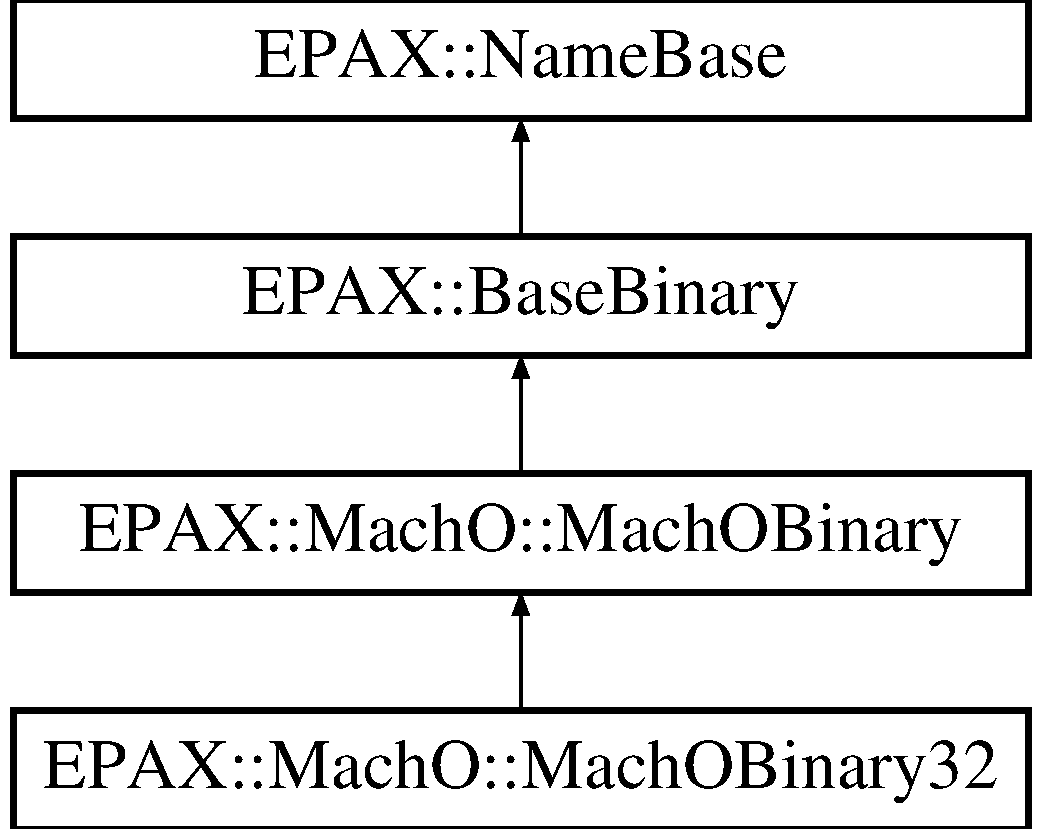
\includegraphics[height=4.000000cm]{class_e_p_a_x_1_1_mach_o_1_1_mach_o_binary32}
\end{center}
\end{figure}
\subsection*{\-Public \-Member \-Functions}
\begin{DoxyCompactItemize}
\item 
\hyperlink{class_e_p_a_x_1_1_mach_o_1_1_mach_o_binary32_afa9f9ebb9a5767c61ed434895bb54c6d}{\-Mach\-O\-Binary32} (std\-::string n)
\item 
virtual \hyperlink{class_e_p_a_x_1_1_mach_o_1_1_mach_o_binary32_abf8ad43c31531cfb3b71e5acda25b3cb}{$\sim$\-Mach\-O\-Binary32} ()
\item 
\hyperlink{namespace_e_p_a_x_a4be639c006ef14def4708b37ee6dd67d}{\-Binary\-Format} \hyperlink{class_e_p_a_x_1_1_mach_o_1_1_mach_o_binary32_a37eab3a09ee0f670f2633a56c890100e}{get\-Format} ()
\end{DoxyCompactItemize}


\subsection{\-Detailed \-Description}


\-Definition at line 69 of file \-Mach\-O\-Binary.\-hpp.



\subsection{\-Constructor \& \-Destructor \-Documentation}
\hypertarget{class_e_p_a_x_1_1_mach_o_1_1_mach_o_binary32_afa9f9ebb9a5767c61ed434895bb54c6d}{\index{\-E\-P\-A\-X\-::\-Mach\-O\-::\-Mach\-O\-Binary32@{\-E\-P\-A\-X\-::\-Mach\-O\-::\-Mach\-O\-Binary32}!\-Mach\-O\-Binary32@{\-Mach\-O\-Binary32}}
\index{\-Mach\-O\-Binary32@{\-Mach\-O\-Binary32}!EPAX::MachO::MachOBinary32@{\-E\-P\-A\-X\-::\-Mach\-O\-::\-Mach\-O\-Binary32}}
\subsubsection[{\-Mach\-O\-Binary32}]{\setlength{\rightskip}{0pt plus 5cm}{\bf \-E\-P\-A\-X\-::\-Mach\-O\-::\-Mach\-O\-Binary32\-::\-Mach\-O\-Binary32} (
\begin{DoxyParamCaption}
\item[{std\-::string}]{n}
\end{DoxyParamCaption}
)}}\label{class_e_p_a_x_1_1_mach_o_1_1_mach_o_binary32_afa9f9ebb9a5767c61ed434895bb54c6d}


\-Definition at line 71 of file \-Mach\-O\-Binary.\-cpp.

\hypertarget{class_e_p_a_x_1_1_mach_o_1_1_mach_o_binary32_abf8ad43c31531cfb3b71e5acda25b3cb}{\index{\-E\-P\-A\-X\-::\-Mach\-O\-::\-Mach\-O\-Binary32@{\-E\-P\-A\-X\-::\-Mach\-O\-::\-Mach\-O\-Binary32}!$\sim$\-Mach\-O\-Binary32@{$\sim$\-Mach\-O\-Binary32}}
\index{$\sim$\-Mach\-O\-Binary32@{$\sim$\-Mach\-O\-Binary32}!EPAX::MachO::MachOBinary32@{\-E\-P\-A\-X\-::\-Mach\-O\-::\-Mach\-O\-Binary32}}
\subsubsection[{$\sim$\-Mach\-O\-Binary32}]{\setlength{\rightskip}{0pt plus 5cm}virtual {\bf \-E\-P\-A\-X\-::\-Mach\-O\-::\-Mach\-O\-Binary32\-::$\sim$\-Mach\-O\-Binary32} (
\begin{DoxyParamCaption}
{}
\end{DoxyParamCaption}
)\hspace{0.3cm}{\ttfamily  \mbox{[}inline, virtual\mbox{]}}}}\label{class_e_p_a_x_1_1_mach_o_1_1_mach_o_binary32_abf8ad43c31531cfb3b71e5acda25b3cb}


\-Definition at line 72 of file \-Mach\-O\-Binary.\-hpp.



\subsection{\-Member \-Function \-Documentation}
\hypertarget{class_e_p_a_x_1_1_mach_o_1_1_mach_o_binary32_a37eab3a09ee0f670f2633a56c890100e}{\index{\-E\-P\-A\-X\-::\-Mach\-O\-::\-Mach\-O\-Binary32@{\-E\-P\-A\-X\-::\-Mach\-O\-::\-Mach\-O\-Binary32}!get\-Format@{get\-Format}}
\index{get\-Format@{get\-Format}!EPAX::MachO::MachOBinary32@{\-E\-P\-A\-X\-::\-Mach\-O\-::\-Mach\-O\-Binary32}}
\subsubsection[{get\-Format}]{\setlength{\rightskip}{0pt plus 5cm}{\bf \-Binary\-Format} {\bf \-E\-P\-A\-X\-::\-Mach\-O\-::\-Mach\-O\-Binary32\-::get\-Format} (
\begin{DoxyParamCaption}
{}
\end{DoxyParamCaption}
)\hspace{0.3cm}{\ttfamily  \mbox{[}inline, virtual\mbox{]}}}}\label{class_e_p_a_x_1_1_mach_o_1_1_mach_o_binary32_a37eab3a09ee0f670f2633a56c890100e}


\-Implements \hyperlink{class_e_p_a_x_1_1_mach_o_1_1_mach_o_binary_a435106c1f40d1ec16ac539fbdecd88bd}{\-E\-P\-A\-X\-::\-Mach\-O\-::\-Mach\-O\-Binary}.



\-Definition at line 74 of file \-Mach\-O\-Binary.\-hpp.



\-The documentation for this class was generated from the following files\-:\begin{DoxyCompactItemize}
\item 
\hyperlink{_mach_o_binary_8hpp}{\-Mach\-O\-Binary.\-hpp}\item 
\hyperlink{_mach_o_binary_8cpp}{\-Mach\-O\-Binary.\-cpp}\end{DoxyCompactItemize}

\hypertarget{class_e_p_a_x_1_1_mach_o_1_1_mach_o_binary64}{\section{\-E\-P\-A\-X\-:\-:\-Mach\-O\-:\-:\-Mach\-O\-Binary64 \-Class \-Reference}
\label{class_e_p_a_x_1_1_mach_o_1_1_mach_o_binary64}\index{\-E\-P\-A\-X\-::\-Mach\-O\-::\-Mach\-O\-Binary64@{\-E\-P\-A\-X\-::\-Mach\-O\-::\-Mach\-O\-Binary64}}
}


{\ttfamily \#include $<$\-Mach\-O\-Binary.\-hpp$>$}

\-Inheritance diagram for \-E\-P\-A\-X\-:\-:\-Mach\-O\-:\-:\-Mach\-O\-Binary64\-:\begin{figure}[H]
\begin{center}
\leavevmode
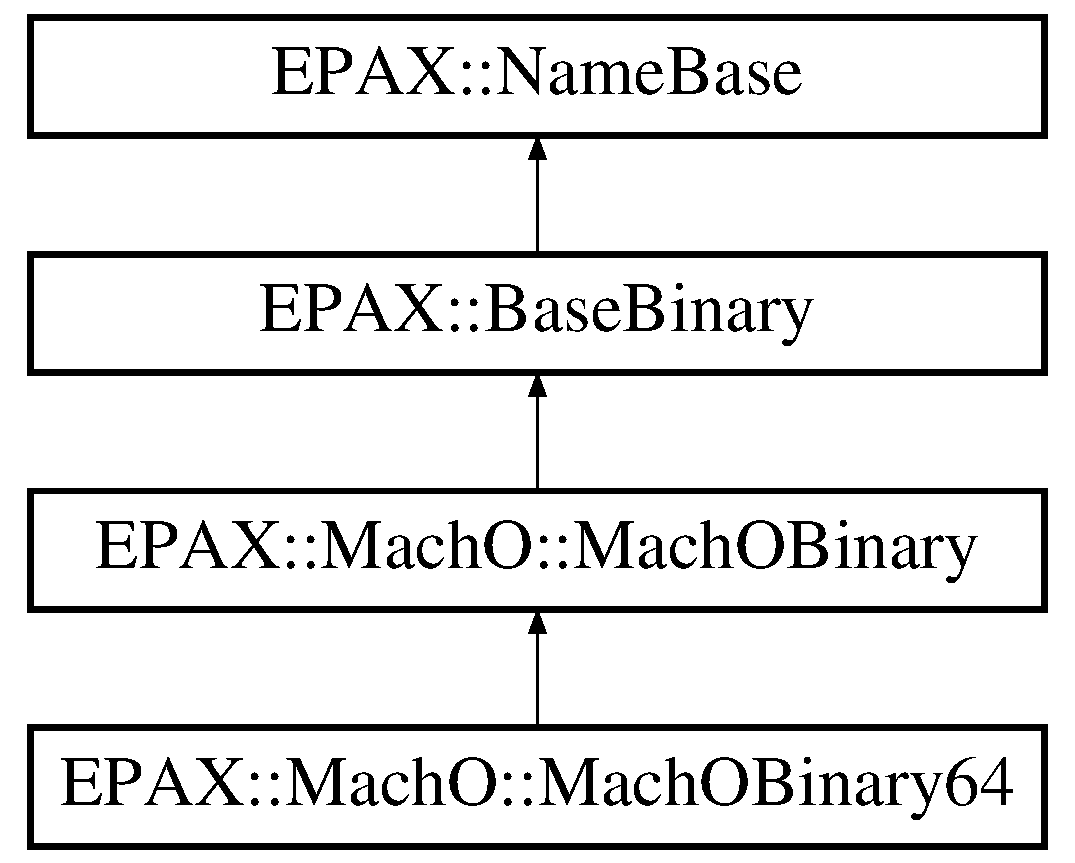
\includegraphics[height=4.000000cm]{class_e_p_a_x_1_1_mach_o_1_1_mach_o_binary64}
\end{center}
\end{figure}
\subsection*{\-Public \-Member \-Functions}
\begin{DoxyCompactItemize}
\item 
\hyperlink{class_e_p_a_x_1_1_mach_o_1_1_mach_o_binary64_a53cd5a142c8aad603e2dec433a22d55d}{\-Mach\-O\-Binary64} (std\-::string n)
\item 
virtual \hyperlink{class_e_p_a_x_1_1_mach_o_1_1_mach_o_binary64_a306f38371fc7cbaffad6a5e8768cfc3b}{$\sim$\-Mach\-O\-Binary64} ()
\item 
\hyperlink{namespace_e_p_a_x_a4be639c006ef14def4708b37ee6dd67d}{\-Binary\-Format} \hyperlink{class_e_p_a_x_1_1_mach_o_1_1_mach_o_binary64_ab2aa03d22ba0339c415a9dc9e6a0912b}{get\-Format} ()
\end{DoxyCompactItemize}


\subsection{\-Detailed \-Description}


\-Definition at line 77 of file \-Mach\-O\-Binary.\-hpp.



\subsection{\-Constructor \& \-Destructor \-Documentation}
\hypertarget{class_e_p_a_x_1_1_mach_o_1_1_mach_o_binary64_a53cd5a142c8aad603e2dec433a22d55d}{\index{\-E\-P\-A\-X\-::\-Mach\-O\-::\-Mach\-O\-Binary64@{\-E\-P\-A\-X\-::\-Mach\-O\-::\-Mach\-O\-Binary64}!\-Mach\-O\-Binary64@{\-Mach\-O\-Binary64}}
\index{\-Mach\-O\-Binary64@{\-Mach\-O\-Binary64}!EPAX::MachO::MachOBinary64@{\-E\-P\-A\-X\-::\-Mach\-O\-::\-Mach\-O\-Binary64}}
\subsubsection[{\-Mach\-O\-Binary64}]{\setlength{\rightskip}{0pt plus 5cm}{\bf \-E\-P\-A\-X\-::\-Mach\-O\-::\-Mach\-O\-Binary64\-::\-Mach\-O\-Binary64} (
\begin{DoxyParamCaption}
\item[{std\-::string}]{n}
\end{DoxyParamCaption}
)}}\label{class_e_p_a_x_1_1_mach_o_1_1_mach_o_binary64_a53cd5a142c8aad603e2dec433a22d55d}


\-Definition at line 77 of file \-Mach\-O\-Binary.\-cpp.

\hypertarget{class_e_p_a_x_1_1_mach_o_1_1_mach_o_binary64_a306f38371fc7cbaffad6a5e8768cfc3b}{\index{\-E\-P\-A\-X\-::\-Mach\-O\-::\-Mach\-O\-Binary64@{\-E\-P\-A\-X\-::\-Mach\-O\-::\-Mach\-O\-Binary64}!$\sim$\-Mach\-O\-Binary64@{$\sim$\-Mach\-O\-Binary64}}
\index{$\sim$\-Mach\-O\-Binary64@{$\sim$\-Mach\-O\-Binary64}!EPAX::MachO::MachOBinary64@{\-E\-P\-A\-X\-::\-Mach\-O\-::\-Mach\-O\-Binary64}}
\subsubsection[{$\sim$\-Mach\-O\-Binary64}]{\setlength{\rightskip}{0pt plus 5cm}virtual {\bf \-E\-P\-A\-X\-::\-Mach\-O\-::\-Mach\-O\-Binary64\-::$\sim$\-Mach\-O\-Binary64} (
\begin{DoxyParamCaption}
{}
\end{DoxyParamCaption}
)\hspace{0.3cm}{\ttfamily  \mbox{[}inline, virtual\mbox{]}}}}\label{class_e_p_a_x_1_1_mach_o_1_1_mach_o_binary64_a306f38371fc7cbaffad6a5e8768cfc3b}


\-Definition at line 80 of file \-Mach\-O\-Binary.\-hpp.



\subsection{\-Member \-Function \-Documentation}
\hypertarget{class_e_p_a_x_1_1_mach_o_1_1_mach_o_binary64_ab2aa03d22ba0339c415a9dc9e6a0912b}{\index{\-E\-P\-A\-X\-::\-Mach\-O\-::\-Mach\-O\-Binary64@{\-E\-P\-A\-X\-::\-Mach\-O\-::\-Mach\-O\-Binary64}!get\-Format@{get\-Format}}
\index{get\-Format@{get\-Format}!EPAX::MachO::MachOBinary64@{\-E\-P\-A\-X\-::\-Mach\-O\-::\-Mach\-O\-Binary64}}
\subsubsection[{get\-Format}]{\setlength{\rightskip}{0pt plus 5cm}{\bf \-Binary\-Format} {\bf \-E\-P\-A\-X\-::\-Mach\-O\-::\-Mach\-O\-Binary64\-::get\-Format} (
\begin{DoxyParamCaption}
{}
\end{DoxyParamCaption}
)\hspace{0.3cm}{\ttfamily  \mbox{[}inline, virtual\mbox{]}}}}\label{class_e_p_a_x_1_1_mach_o_1_1_mach_o_binary64_ab2aa03d22ba0339c415a9dc9e6a0912b}


\-Implements \hyperlink{class_e_p_a_x_1_1_mach_o_1_1_mach_o_binary_a435106c1f40d1ec16ac539fbdecd88bd}{\-E\-P\-A\-X\-::\-Mach\-O\-::\-Mach\-O\-Binary}.



\-Definition at line 82 of file \-Mach\-O\-Binary.\-hpp.



\-The documentation for this class was generated from the following files\-:\begin{DoxyCompactItemize}
\item 
\hyperlink{_mach_o_binary_8hpp}{\-Mach\-O\-Binary.\-hpp}\item 
\hyperlink{_mach_o_binary_8cpp}{\-Mach\-O\-Binary.\-cpp}\end{DoxyCompactItemize}

\hypertarget{class_e_p_a_x_1_1_memory_base}{\section{\-E\-P\-A\-X\-:\-:\-Memory\-Base \-Class \-Reference}
\label{class_e_p_a_x_1_1_memory_base}\index{\-E\-P\-A\-X\-::\-Memory\-Base@{\-E\-P\-A\-X\-::\-Memory\-Base}}
}


{\ttfamily \#include $<$\-Base\-Class.\-hpp$>$}

\-Inheritance diagram for \-E\-P\-A\-X\-:\-:\-Memory\-Base\-:\begin{figure}[H]
\begin{center}
\leavevmode
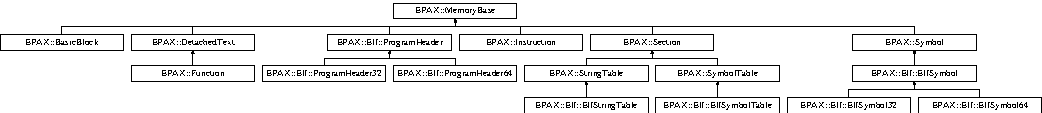
\includegraphics[height=1.513514cm]{class_e_p_a_x_1_1_memory_base}
\end{center}
\end{figure}
\subsection*{\-Public \-Member \-Functions}
\begin{DoxyCompactItemize}
\item 
\hyperlink{class_e_p_a_x_1_1_memory_base_aab70a4cec3d7a6386cc02f3ea7475335}{\-Memory\-Base} (uint64\-\_\-t a, uint64\-\_\-t s)
\item 
\hyperlink{class_e_p_a_x_1_1_memory_base_a8a9e77bc67627ef0c1655b7aa9510e95}{\-Memory\-Base} ()
\item 
virtual \hyperlink{class_e_p_a_x_1_1_memory_base_a1b771e1cdf376ee2960bf7a6947fe110}{$\sim$\-Memory\-Base} ()
\item 
uint64\-\_\-t \hyperlink{class_e_p_a_x_1_1_memory_base_afecca3bccbbf4d19d16bc2490ad086ca}{get\-Memory\-Address} ()
\item 
uint64\-\_\-t \hyperlink{class_e_p_a_x_1_1_memory_base_aac80cc9059e3f458027a22eb5ea59e01}{get\-Memory\-Size} ()
\item 
void \hyperlink{class_e_p_a_x_1_1_memory_base_ae39b6d63f7791f5192c9cb9a28b4a218}{set\-Memory\-Size} (uint64\-\_\-t s)
\item 
bool \hyperlink{class_e_p_a_x_1_1_memory_base_a2491f4748c4c0aa3311e586919730e3e}{in\-Range} (uint64\-\_\-t a)
\end{DoxyCompactItemize}


\subsection{\-Detailed \-Description}


\-Definition at line 61 of file \-Base\-Class.\-hpp.



\subsection{\-Constructor \& \-Destructor \-Documentation}
\hypertarget{class_e_p_a_x_1_1_memory_base_aab70a4cec3d7a6386cc02f3ea7475335}{\index{\-E\-P\-A\-X\-::\-Memory\-Base@{\-E\-P\-A\-X\-::\-Memory\-Base}!\-Memory\-Base@{\-Memory\-Base}}
\index{\-Memory\-Base@{\-Memory\-Base}!EPAX::MemoryBase@{\-E\-P\-A\-X\-::\-Memory\-Base}}
\subsubsection[{\-Memory\-Base}]{\setlength{\rightskip}{0pt plus 5cm}{\bf \-E\-P\-A\-X\-::\-Memory\-Base\-::\-Memory\-Base} (
\begin{DoxyParamCaption}
\item[{uint64\-\_\-t}]{a, }
\item[{uint64\-\_\-t}]{s}
\end{DoxyParamCaption}
)\hspace{0.3cm}{\ttfamily  \mbox{[}inline\mbox{]}}}}\label{class_e_p_a_x_1_1_memory_base_aab70a4cec3d7a6386cc02f3ea7475335}


\-Definition at line 67 of file \-Base\-Class.\-hpp.

\hypertarget{class_e_p_a_x_1_1_memory_base_a8a9e77bc67627ef0c1655b7aa9510e95}{\index{\-E\-P\-A\-X\-::\-Memory\-Base@{\-E\-P\-A\-X\-::\-Memory\-Base}!\-Memory\-Base@{\-Memory\-Base}}
\index{\-Memory\-Base@{\-Memory\-Base}!EPAX::MemoryBase@{\-E\-P\-A\-X\-::\-Memory\-Base}}
\subsubsection[{\-Memory\-Base}]{\setlength{\rightskip}{0pt plus 5cm}{\bf \-E\-P\-A\-X\-::\-Memory\-Base\-::\-Memory\-Base} (
\begin{DoxyParamCaption}
{}
\end{DoxyParamCaption}
)\hspace{0.3cm}{\ttfamily  \mbox{[}inline\mbox{]}}}}\label{class_e_p_a_x_1_1_memory_base_a8a9e77bc67627ef0c1655b7aa9510e95}


\-Definition at line 69 of file \-Base\-Class.\-hpp.

\hypertarget{class_e_p_a_x_1_1_memory_base_a1b771e1cdf376ee2960bf7a6947fe110}{\index{\-E\-P\-A\-X\-::\-Memory\-Base@{\-E\-P\-A\-X\-::\-Memory\-Base}!$\sim$\-Memory\-Base@{$\sim$\-Memory\-Base}}
\index{$\sim$\-Memory\-Base@{$\sim$\-Memory\-Base}!EPAX::MemoryBase@{\-E\-P\-A\-X\-::\-Memory\-Base}}
\subsubsection[{$\sim$\-Memory\-Base}]{\setlength{\rightskip}{0pt plus 5cm}virtual {\bf \-E\-P\-A\-X\-::\-Memory\-Base\-::$\sim$\-Memory\-Base} (
\begin{DoxyParamCaption}
{}
\end{DoxyParamCaption}
)\hspace{0.3cm}{\ttfamily  \mbox{[}inline, virtual\mbox{]}}}}\label{class_e_p_a_x_1_1_memory_base_a1b771e1cdf376ee2960bf7a6947fe110}


\-Definition at line 71 of file \-Base\-Class.\-hpp.



\subsection{\-Member \-Function \-Documentation}
\hypertarget{class_e_p_a_x_1_1_memory_base_afecca3bccbbf4d19d16bc2490ad086ca}{\index{\-E\-P\-A\-X\-::\-Memory\-Base@{\-E\-P\-A\-X\-::\-Memory\-Base}!get\-Memory\-Address@{get\-Memory\-Address}}
\index{get\-Memory\-Address@{get\-Memory\-Address}!EPAX::MemoryBase@{\-E\-P\-A\-X\-::\-Memory\-Base}}
\subsubsection[{get\-Memory\-Address}]{\setlength{\rightskip}{0pt plus 5cm}uint64\-\_\-t {\bf \-E\-P\-A\-X\-::\-Memory\-Base\-::get\-Memory\-Address} (
\begin{DoxyParamCaption}
{}
\end{DoxyParamCaption}
)\hspace{0.3cm}{\ttfamily  \mbox{[}inline\mbox{]}}}}\label{class_e_p_a_x_1_1_memory_base_afecca3bccbbf4d19d16bc2490ad086ca}


\-Definition at line 73 of file \-Base\-Class.\-hpp.

\hypertarget{class_e_p_a_x_1_1_memory_base_aac80cc9059e3f458027a22eb5ea59e01}{\index{\-E\-P\-A\-X\-::\-Memory\-Base@{\-E\-P\-A\-X\-::\-Memory\-Base}!get\-Memory\-Size@{get\-Memory\-Size}}
\index{get\-Memory\-Size@{get\-Memory\-Size}!EPAX::MemoryBase@{\-E\-P\-A\-X\-::\-Memory\-Base}}
\subsubsection[{get\-Memory\-Size}]{\setlength{\rightskip}{0pt plus 5cm}uint64\-\_\-t {\bf \-E\-P\-A\-X\-::\-Memory\-Base\-::get\-Memory\-Size} (
\begin{DoxyParamCaption}
{}
\end{DoxyParamCaption}
)\hspace{0.3cm}{\ttfamily  \mbox{[}inline\mbox{]}}}}\label{class_e_p_a_x_1_1_memory_base_aac80cc9059e3f458027a22eb5ea59e01}


\-Definition at line 74 of file \-Base\-Class.\-hpp.

\hypertarget{class_e_p_a_x_1_1_memory_base_a2491f4748c4c0aa3311e586919730e3e}{\index{\-E\-P\-A\-X\-::\-Memory\-Base@{\-E\-P\-A\-X\-::\-Memory\-Base}!in\-Range@{in\-Range}}
\index{in\-Range@{in\-Range}!EPAX::MemoryBase@{\-E\-P\-A\-X\-::\-Memory\-Base}}
\subsubsection[{in\-Range}]{\setlength{\rightskip}{0pt plus 5cm}bool {\bf \-E\-P\-A\-X\-::\-Memory\-Base\-::in\-Range} (
\begin{DoxyParamCaption}
\item[{uint64\-\_\-t}]{a}
\end{DoxyParamCaption}
)}}\label{class_e_p_a_x_1_1_memory_base_a2491f4748c4c0aa3311e586919730e3e}


\-Definition at line 54 of file \-Base\-Class.\-cpp.

\hypertarget{class_e_p_a_x_1_1_memory_base_ae39b6d63f7791f5192c9cb9a28b4a218}{\index{\-E\-P\-A\-X\-::\-Memory\-Base@{\-E\-P\-A\-X\-::\-Memory\-Base}!set\-Memory\-Size@{set\-Memory\-Size}}
\index{set\-Memory\-Size@{set\-Memory\-Size}!EPAX::MemoryBase@{\-E\-P\-A\-X\-::\-Memory\-Base}}
\subsubsection[{set\-Memory\-Size}]{\setlength{\rightskip}{0pt plus 5cm}void {\bf \-E\-P\-A\-X\-::\-Memory\-Base\-::set\-Memory\-Size} (
\begin{DoxyParamCaption}
\item[{uint64\-\_\-t}]{s}
\end{DoxyParamCaption}
)\hspace{0.3cm}{\ttfamily  \mbox{[}inline\mbox{]}}}}\label{class_e_p_a_x_1_1_memory_base_ae39b6d63f7791f5192c9cb9a28b4a218}


\-Definition at line 75 of file \-Base\-Class.\-hpp.



\-The documentation for this class was generated from the following files\-:\begin{DoxyCompactItemize}
\item 
\hyperlink{_base_class_8hpp}{\-Base\-Class.\-hpp}\item 
\hyperlink{_base_class_8cpp}{\-Base\-Class.\-cpp}\end{DoxyCompactItemize}

\hypertarget{class_e_p_a_x_1_1_name_base}{\section{\-E\-P\-A\-X\-:\-:\-Name\-Base \-Class \-Reference}
\label{class_e_p_a_x_1_1_name_base}\index{\-E\-P\-A\-X\-::\-Name\-Base@{\-E\-P\-A\-X\-::\-Name\-Base}}
}


{\ttfamily \#include $<$\-Base\-Class.\-hpp$>$}

\-Inheritance diagram for \-E\-P\-A\-X\-:\-:\-Name\-Base\-:\begin{figure}[H]
\begin{center}
\leavevmode
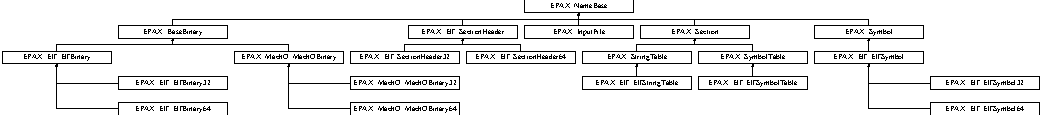
\includegraphics[height=1.547817cm]{class_e_p_a_x_1_1_name_base}
\end{center}
\end{figure}
\subsection*{\-Public \-Member \-Functions}
\begin{DoxyCompactItemize}
\item 
\hyperlink{class_e_p_a_x_1_1_name_base_acdbcff79c1f15eaafdf9dd65a48bc22b}{\-Name\-Base} (std\-::string n)
\item 
\hyperlink{class_e_p_a_x_1_1_name_base_a3b74b295e3e77e0be7fefa482e4452d4}{\-Name\-Base} ()
\item 
virtual \hyperlink{class_e_p_a_x_1_1_name_base_a5de3a56d6fc0d30270b0a32ad81f3c30}{$\sim$\-Name\-Base} ()
\item 
std\-::string \hyperlink{class_e_p_a_x_1_1_name_base_ac45bad0887b6a3283cc76047f91f7708}{get\-Name} ()
\item 
void \hyperlink{class_e_p_a_x_1_1_name_base_a0249989dc06f3563cdee08435856d15d}{set\-Name} (std\-::string n)
\end{DoxyCompactItemize}


\subsection{\-Detailed \-Description}


\-Definition at line 107 of file \-Base\-Class.\-hpp.



\subsection{\-Constructor \& \-Destructor \-Documentation}
\hypertarget{class_e_p_a_x_1_1_name_base_acdbcff79c1f15eaafdf9dd65a48bc22b}{\index{\-E\-P\-A\-X\-::\-Name\-Base@{\-E\-P\-A\-X\-::\-Name\-Base}!\-Name\-Base@{\-Name\-Base}}
\index{\-Name\-Base@{\-Name\-Base}!EPAX::NameBase@{\-E\-P\-A\-X\-::\-Name\-Base}}
\subsubsection[{\-Name\-Base}]{\setlength{\rightskip}{0pt plus 5cm}{\bf \-E\-P\-A\-X\-::\-Name\-Base\-::\-Name\-Base} (
\begin{DoxyParamCaption}
\item[{std\-::string}]{n}
\end{DoxyParamCaption}
)\hspace{0.3cm}{\ttfamily  \mbox{[}inline\mbox{]}}}}\label{class_e_p_a_x_1_1_name_base_acdbcff79c1f15eaafdf9dd65a48bc22b}


\-Definition at line 112 of file \-Base\-Class.\-hpp.

\hypertarget{class_e_p_a_x_1_1_name_base_a3b74b295e3e77e0be7fefa482e4452d4}{\index{\-E\-P\-A\-X\-::\-Name\-Base@{\-E\-P\-A\-X\-::\-Name\-Base}!\-Name\-Base@{\-Name\-Base}}
\index{\-Name\-Base@{\-Name\-Base}!EPAX::NameBase@{\-E\-P\-A\-X\-::\-Name\-Base}}
\subsubsection[{\-Name\-Base}]{\setlength{\rightskip}{0pt plus 5cm}{\bf \-E\-P\-A\-X\-::\-Name\-Base\-::\-Name\-Base} (
\begin{DoxyParamCaption}
{}
\end{DoxyParamCaption}
)\hspace{0.3cm}{\ttfamily  \mbox{[}inline\mbox{]}}}}\label{class_e_p_a_x_1_1_name_base_a3b74b295e3e77e0be7fefa482e4452d4}


\-Definition at line 113 of file \-Base\-Class.\-hpp.

\hypertarget{class_e_p_a_x_1_1_name_base_a5de3a56d6fc0d30270b0a32ad81f3c30}{\index{\-E\-P\-A\-X\-::\-Name\-Base@{\-E\-P\-A\-X\-::\-Name\-Base}!$\sim$\-Name\-Base@{$\sim$\-Name\-Base}}
\index{$\sim$\-Name\-Base@{$\sim$\-Name\-Base}!EPAX::NameBase@{\-E\-P\-A\-X\-::\-Name\-Base}}
\subsubsection[{$\sim$\-Name\-Base}]{\setlength{\rightskip}{0pt plus 5cm}virtual {\bf \-E\-P\-A\-X\-::\-Name\-Base\-::$\sim$\-Name\-Base} (
\begin{DoxyParamCaption}
{}
\end{DoxyParamCaption}
)\hspace{0.3cm}{\ttfamily  \mbox{[}inline, virtual\mbox{]}}}}\label{class_e_p_a_x_1_1_name_base_a5de3a56d6fc0d30270b0a32ad81f3c30}


\-Definition at line 114 of file \-Base\-Class.\-hpp.



\subsection{\-Member \-Function \-Documentation}
\hypertarget{class_e_p_a_x_1_1_name_base_ac45bad0887b6a3283cc76047f91f7708}{\index{\-E\-P\-A\-X\-::\-Name\-Base@{\-E\-P\-A\-X\-::\-Name\-Base}!get\-Name@{get\-Name}}
\index{get\-Name@{get\-Name}!EPAX::NameBase@{\-E\-P\-A\-X\-::\-Name\-Base}}
\subsubsection[{get\-Name}]{\setlength{\rightskip}{0pt plus 5cm}std\-::string {\bf \-E\-P\-A\-X\-::\-Name\-Base\-::get\-Name} (
\begin{DoxyParamCaption}
{}
\end{DoxyParamCaption}
)\hspace{0.3cm}{\ttfamily  \mbox{[}inline\mbox{]}}}}\label{class_e_p_a_x_1_1_name_base_ac45bad0887b6a3283cc76047f91f7708}


\-Definition at line 116 of file \-Base\-Class.\-hpp.

\hypertarget{class_e_p_a_x_1_1_name_base_a0249989dc06f3563cdee08435856d15d}{\index{\-E\-P\-A\-X\-::\-Name\-Base@{\-E\-P\-A\-X\-::\-Name\-Base}!set\-Name@{set\-Name}}
\index{set\-Name@{set\-Name}!EPAX::NameBase@{\-E\-P\-A\-X\-::\-Name\-Base}}
\subsubsection[{set\-Name}]{\setlength{\rightskip}{0pt plus 5cm}void {\bf \-E\-P\-A\-X\-::\-Name\-Base\-::set\-Name} (
\begin{DoxyParamCaption}
\item[{std\-::string}]{n}
\end{DoxyParamCaption}
)\hspace{0.3cm}{\ttfamily  \mbox{[}inline\mbox{]}}}}\label{class_e_p_a_x_1_1_name_base_a0249989dc06f3563cdee08435856d15d}


\-Definition at line 117 of file \-Base\-Class.\-hpp.



\-The documentation for this class was generated from the following file\-:\begin{DoxyCompactItemize}
\item 
\hyperlink{_base_class_8hpp}{\-Base\-Class.\-hpp}\end{DoxyCompactItemize}

\hypertarget{class_e_p_a_x_1_1_elf_1_1_program_header}{\section{\-E\-P\-A\-X\-:\-:\-Elf\-:\-:\-Program\-Header \-Class \-Reference}
\label{class_e_p_a_x_1_1_elf_1_1_program_header}\index{\-E\-P\-A\-X\-::\-Elf\-::\-Program\-Header@{\-E\-P\-A\-X\-::\-Elf\-::\-Program\-Header}}
}


{\ttfamily \#include $<$\-Elf\-Binary.\-hpp$>$}

\-Inheritance diagram for \-E\-P\-A\-X\-:\-:\-Elf\-:\-:\-Program\-Header\-:\begin{figure}[H]
\begin{center}
\leavevmode
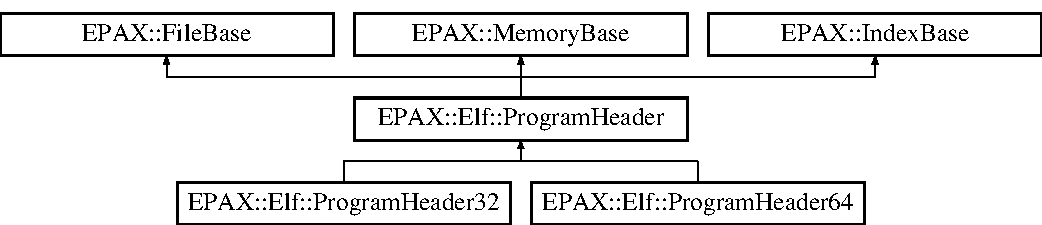
\includegraphics[height=3.000000cm]{class_e_p_a_x_1_1_elf_1_1_program_header}
\end{center}
\end{figure}
\subsection*{\-Public \-Member \-Functions}
\begin{DoxyCompactItemize}
\item 
\hyperlink{class_e_p_a_x_1_1_elf_1_1_program_header_a3696fa6a32c99da64d87a686a881fe9a}{\-Program\-Header} (\hyperlink{class_e_p_a_x_1_1_base_binary}{\-Base\-Binary} $\ast$b, uint64\-\_\-t o, uint64\-\_\-t s, uint32\-\_\-t i)
\item 
virtual \hyperlink{class_e_p_a_x_1_1_elf_1_1_program_header_a9da71f94c2c142aafde175151d48937f}{$\sim$\-Program\-Header} ()
\item 
bool \hyperlink{class_e_p_a_x_1_1_elf_1_1_program_header_ae31e5d8dba8226b42315bcfa28b5d596}{is\-Valid\-Vaddr} (uint64\-\_\-t v)
\item 
uint64\-\_\-t \hyperlink{class_e_p_a_x_1_1_elf_1_1_program_header_a42aab9c522155567f18175b1f09d4d3c}{vaddr\-To\-Fileaddr} (uint64\-\_\-t v)
\item 
virtual uint64\-\_\-t \hyperlink{class_e_p_a_x_1_1_elf_1_1_program_header_aa8a7d552ece248bccfda3d320fe2d2ab}{get\-Vaddr} ()=0
\item 
virtual uint64\-\_\-t \hyperlink{class_e_p_a_x_1_1_elf_1_1_program_header_aff0f58569378cdcb6c4d7ab309af62c7}{get\-Paddr} ()=0
\item 
virtual uint64\-\_\-t \hyperlink{class_e_p_a_x_1_1_elf_1_1_program_header_aa0dfb27d2bb6b869c2810c2ee070ff7b}{get\-F\-Size} ()=0
\item 
virtual uint64\-\_\-t \hyperlink{class_e_p_a_x_1_1_elf_1_1_program_header_ab624186a1963231b21722025d9f87a32}{get\-M\-Size} ()=0
\item 
virtual uint32\-\_\-t \hyperlink{class_e_p_a_x_1_1_elf_1_1_program_header_a2034c6e8212ac3ced6719a706b48d6d1}{get\-Segment\-Type} ()=0
\item 
virtual uint64\-\_\-t \hyperlink{class_e_p_a_x_1_1_elf_1_1_program_header_a566bcceecb66e2b159e3e52b44e2f941}{get\-Flags} ()=0
\item 
virtual uint32\-\_\-t \hyperlink{class_e_p_a_x_1_1_elf_1_1_program_header_acfef642e82022bdd883944e48dff4015}{get\-Alignment} ()=0
\item 
virtual uint64\-\_\-t \hyperlink{class_e_p_a_x_1_1_elf_1_1_program_header_a328166b748f2717c9da393210f7aa9cc}{get\-F\-Offset} ()=0
\end{DoxyCompactItemize}
\subsection*{\-Protected \-Attributes}
\begin{DoxyCompactItemize}
\item 
\hyperlink{_e_p_a_x_common_internal_8hpp_a17755bdd71c02e656c667b16de61dd7b}{rawbyte\-\_\-t} $\ast$ \hyperlink{class_e_p_a_x_1_1_elf_1_1_program_header_a25865997e5c358b60ff630a68494c89c}{entry}
\end{DoxyCompactItemize}


\subsection{\-Detailed \-Description}


\-Definition at line 319 of file \-Elf\-Binary.\-hpp.



\subsection{\-Constructor \& \-Destructor \-Documentation}
\hypertarget{class_e_p_a_x_1_1_elf_1_1_program_header_a3696fa6a32c99da64d87a686a881fe9a}{\index{\-E\-P\-A\-X\-::\-Elf\-::\-Program\-Header@{\-E\-P\-A\-X\-::\-Elf\-::\-Program\-Header}!\-Program\-Header@{\-Program\-Header}}
\index{\-Program\-Header@{\-Program\-Header}!EPAX::Elf::ProgramHeader@{\-E\-P\-A\-X\-::\-Elf\-::\-Program\-Header}}
\subsubsection[{\-Program\-Header}]{\setlength{\rightskip}{0pt plus 5cm}{\bf \-E\-P\-A\-X\-::\-Elf\-::\-Program\-Header\-::\-Program\-Header} (
\begin{DoxyParamCaption}
\item[{{\bf \-Base\-Binary} $\ast$}]{b, }
\item[{uint64\-\_\-t}]{o, }
\item[{uint64\-\_\-t}]{s, }
\item[{uint32\-\_\-t}]{i}
\end{DoxyParamCaption}
)}}\label{class_e_p_a_x_1_1_elf_1_1_program_header_a3696fa6a32c99da64d87a686a881fe9a}


\-Definition at line 691 of file \-Elf\-Binary.\-cpp.

\hypertarget{class_e_p_a_x_1_1_elf_1_1_program_header_a9da71f94c2c142aafde175151d48937f}{\index{\-E\-P\-A\-X\-::\-Elf\-::\-Program\-Header@{\-E\-P\-A\-X\-::\-Elf\-::\-Program\-Header}!$\sim$\-Program\-Header@{$\sim$\-Program\-Header}}
\index{$\sim$\-Program\-Header@{$\sim$\-Program\-Header}!EPAX::Elf::ProgramHeader@{\-E\-P\-A\-X\-::\-Elf\-::\-Program\-Header}}
\subsubsection[{$\sim$\-Program\-Header}]{\setlength{\rightskip}{0pt plus 5cm}{\bf \-E\-P\-A\-X\-::\-Elf\-::\-Program\-Header\-::$\sim$\-Program\-Header} (
\begin{DoxyParamCaption}
{}
\end{DoxyParamCaption}
)\hspace{0.3cm}{\ttfamily  \mbox{[}virtual\mbox{]}}}}\label{class_e_p_a_x_1_1_elf_1_1_program_header_a9da71f94c2c142aafde175151d48937f}


\-Definition at line 698 of file \-Elf\-Binary.\-cpp.



\subsection{\-Member \-Function \-Documentation}
\hypertarget{class_e_p_a_x_1_1_elf_1_1_program_header_acfef642e82022bdd883944e48dff4015}{\index{\-E\-P\-A\-X\-::\-Elf\-::\-Program\-Header@{\-E\-P\-A\-X\-::\-Elf\-::\-Program\-Header}!get\-Alignment@{get\-Alignment}}
\index{get\-Alignment@{get\-Alignment}!EPAX::Elf::ProgramHeader@{\-E\-P\-A\-X\-::\-Elf\-::\-Program\-Header}}
\subsubsection[{get\-Alignment}]{\setlength{\rightskip}{0pt plus 5cm}virtual uint32\-\_\-t {\bf \-E\-P\-A\-X\-::\-Elf\-::\-Program\-Header\-::get\-Alignment} (
\begin{DoxyParamCaption}
{}
\end{DoxyParamCaption}
)\hspace{0.3cm}{\ttfamily  \mbox{[}pure virtual\mbox{]}}}}\label{class_e_p_a_x_1_1_elf_1_1_program_header_acfef642e82022bdd883944e48dff4015}


\-Implemented in \hyperlink{class_e_p_a_x_1_1_elf_1_1_program_header64_a68a761d44891ce538049b04236fe2a9c}{\-E\-P\-A\-X\-::\-Elf\-::\-Program\-Header64}, and \hyperlink{class_e_p_a_x_1_1_elf_1_1_program_header32_a8b50e70db41f7b4f646f1ab2b54c227a}{\-E\-P\-A\-X\-::\-Elf\-::\-Program\-Header32}.

\hypertarget{class_e_p_a_x_1_1_elf_1_1_program_header_a566bcceecb66e2b159e3e52b44e2f941}{\index{\-E\-P\-A\-X\-::\-Elf\-::\-Program\-Header@{\-E\-P\-A\-X\-::\-Elf\-::\-Program\-Header}!get\-Flags@{get\-Flags}}
\index{get\-Flags@{get\-Flags}!EPAX::Elf::ProgramHeader@{\-E\-P\-A\-X\-::\-Elf\-::\-Program\-Header}}
\subsubsection[{get\-Flags}]{\setlength{\rightskip}{0pt plus 5cm}virtual uint64\-\_\-t {\bf \-E\-P\-A\-X\-::\-Elf\-::\-Program\-Header\-::get\-Flags} (
\begin{DoxyParamCaption}
{}
\end{DoxyParamCaption}
)\hspace{0.3cm}{\ttfamily  \mbox{[}pure virtual\mbox{]}}}}\label{class_e_p_a_x_1_1_elf_1_1_program_header_a566bcceecb66e2b159e3e52b44e2f941}


\-Implemented in \hyperlink{class_e_p_a_x_1_1_elf_1_1_program_header64_a9f12ad0de269ad3c5c7f2fc52f72fc5a}{\-E\-P\-A\-X\-::\-Elf\-::\-Program\-Header64}, and \hyperlink{class_e_p_a_x_1_1_elf_1_1_program_header32_ac97782a148e1eacf90b38720e535cbef}{\-E\-P\-A\-X\-::\-Elf\-::\-Program\-Header32}.

\hypertarget{class_e_p_a_x_1_1_elf_1_1_program_header_a328166b748f2717c9da393210f7aa9cc}{\index{\-E\-P\-A\-X\-::\-Elf\-::\-Program\-Header@{\-E\-P\-A\-X\-::\-Elf\-::\-Program\-Header}!get\-F\-Offset@{get\-F\-Offset}}
\index{get\-F\-Offset@{get\-F\-Offset}!EPAX::Elf::ProgramHeader@{\-E\-P\-A\-X\-::\-Elf\-::\-Program\-Header}}
\subsubsection[{get\-F\-Offset}]{\setlength{\rightskip}{0pt plus 5cm}virtual uint64\-\_\-t {\bf \-E\-P\-A\-X\-::\-Elf\-::\-Program\-Header\-::get\-F\-Offset} (
\begin{DoxyParamCaption}
{}
\end{DoxyParamCaption}
)\hspace{0.3cm}{\ttfamily  \mbox{[}pure virtual\mbox{]}}}}\label{class_e_p_a_x_1_1_elf_1_1_program_header_a328166b748f2717c9da393210f7aa9cc}


\-Implemented in \hyperlink{class_e_p_a_x_1_1_elf_1_1_program_header64_adde9f4fb75d093fcc7f30d42909f8ef5}{\-E\-P\-A\-X\-::\-Elf\-::\-Program\-Header64}, and \hyperlink{class_e_p_a_x_1_1_elf_1_1_program_header32_a46bdc77ad9a585e058f0dadcc4e71831}{\-E\-P\-A\-X\-::\-Elf\-::\-Program\-Header32}.

\hypertarget{class_e_p_a_x_1_1_elf_1_1_program_header_aa0dfb27d2bb6b869c2810c2ee070ff7b}{\index{\-E\-P\-A\-X\-::\-Elf\-::\-Program\-Header@{\-E\-P\-A\-X\-::\-Elf\-::\-Program\-Header}!get\-F\-Size@{get\-F\-Size}}
\index{get\-F\-Size@{get\-F\-Size}!EPAX::Elf::ProgramHeader@{\-E\-P\-A\-X\-::\-Elf\-::\-Program\-Header}}
\subsubsection[{get\-F\-Size}]{\setlength{\rightskip}{0pt plus 5cm}virtual uint64\-\_\-t {\bf \-E\-P\-A\-X\-::\-Elf\-::\-Program\-Header\-::get\-F\-Size} (
\begin{DoxyParamCaption}
{}
\end{DoxyParamCaption}
)\hspace{0.3cm}{\ttfamily  \mbox{[}pure virtual\mbox{]}}}}\label{class_e_p_a_x_1_1_elf_1_1_program_header_aa0dfb27d2bb6b869c2810c2ee070ff7b}


\-Implemented in \hyperlink{class_e_p_a_x_1_1_elf_1_1_program_header64_a04e7b5890ccc7c01d23e221fbfc44708}{\-E\-P\-A\-X\-::\-Elf\-::\-Program\-Header64}, and \hyperlink{class_e_p_a_x_1_1_elf_1_1_program_header32_a8eac270d2eff779a2f7de736f0b77113}{\-E\-P\-A\-X\-::\-Elf\-::\-Program\-Header32}.

\hypertarget{class_e_p_a_x_1_1_elf_1_1_program_header_ab624186a1963231b21722025d9f87a32}{\index{\-E\-P\-A\-X\-::\-Elf\-::\-Program\-Header@{\-E\-P\-A\-X\-::\-Elf\-::\-Program\-Header}!get\-M\-Size@{get\-M\-Size}}
\index{get\-M\-Size@{get\-M\-Size}!EPAX::Elf::ProgramHeader@{\-E\-P\-A\-X\-::\-Elf\-::\-Program\-Header}}
\subsubsection[{get\-M\-Size}]{\setlength{\rightskip}{0pt plus 5cm}virtual uint64\-\_\-t {\bf \-E\-P\-A\-X\-::\-Elf\-::\-Program\-Header\-::get\-M\-Size} (
\begin{DoxyParamCaption}
{}
\end{DoxyParamCaption}
)\hspace{0.3cm}{\ttfamily  \mbox{[}pure virtual\mbox{]}}}}\label{class_e_p_a_x_1_1_elf_1_1_program_header_ab624186a1963231b21722025d9f87a32}


\-Implemented in \hyperlink{class_e_p_a_x_1_1_elf_1_1_program_header64_a821b37a8d6ebdf7fea555e7a4434eac2}{\-E\-P\-A\-X\-::\-Elf\-::\-Program\-Header64}, and \hyperlink{class_e_p_a_x_1_1_elf_1_1_program_header32_a81d8e54c74130cc27f72ceb27a2044af}{\-E\-P\-A\-X\-::\-Elf\-::\-Program\-Header32}.

\hypertarget{class_e_p_a_x_1_1_elf_1_1_program_header_aff0f58569378cdcb6c4d7ab309af62c7}{\index{\-E\-P\-A\-X\-::\-Elf\-::\-Program\-Header@{\-E\-P\-A\-X\-::\-Elf\-::\-Program\-Header}!get\-Paddr@{get\-Paddr}}
\index{get\-Paddr@{get\-Paddr}!EPAX::Elf::ProgramHeader@{\-E\-P\-A\-X\-::\-Elf\-::\-Program\-Header}}
\subsubsection[{get\-Paddr}]{\setlength{\rightskip}{0pt plus 5cm}virtual uint64\-\_\-t {\bf \-E\-P\-A\-X\-::\-Elf\-::\-Program\-Header\-::get\-Paddr} (
\begin{DoxyParamCaption}
{}
\end{DoxyParamCaption}
)\hspace{0.3cm}{\ttfamily  \mbox{[}pure virtual\mbox{]}}}}\label{class_e_p_a_x_1_1_elf_1_1_program_header_aff0f58569378cdcb6c4d7ab309af62c7}


\-Implemented in \hyperlink{class_e_p_a_x_1_1_elf_1_1_program_header64_a7e1bc27b844418b80f56c458a49797a6}{\-E\-P\-A\-X\-::\-Elf\-::\-Program\-Header64}, and \hyperlink{class_e_p_a_x_1_1_elf_1_1_program_header32_a00042a0b2d817185d053d0647956261f}{\-E\-P\-A\-X\-::\-Elf\-::\-Program\-Header32}.

\hypertarget{class_e_p_a_x_1_1_elf_1_1_program_header_a2034c6e8212ac3ced6719a706b48d6d1}{\index{\-E\-P\-A\-X\-::\-Elf\-::\-Program\-Header@{\-E\-P\-A\-X\-::\-Elf\-::\-Program\-Header}!get\-Segment\-Type@{get\-Segment\-Type}}
\index{get\-Segment\-Type@{get\-Segment\-Type}!EPAX::Elf::ProgramHeader@{\-E\-P\-A\-X\-::\-Elf\-::\-Program\-Header}}
\subsubsection[{get\-Segment\-Type}]{\setlength{\rightskip}{0pt plus 5cm}virtual uint32\-\_\-t {\bf \-E\-P\-A\-X\-::\-Elf\-::\-Program\-Header\-::get\-Segment\-Type} (
\begin{DoxyParamCaption}
{}
\end{DoxyParamCaption}
)\hspace{0.3cm}{\ttfamily  \mbox{[}pure virtual\mbox{]}}}}\label{class_e_p_a_x_1_1_elf_1_1_program_header_a2034c6e8212ac3ced6719a706b48d6d1}


\-Implemented in \hyperlink{class_e_p_a_x_1_1_elf_1_1_program_header64_a5a35087dbe63d5fdabd5893bb57c38a3}{\-E\-P\-A\-X\-::\-Elf\-::\-Program\-Header64}, and \hyperlink{class_e_p_a_x_1_1_elf_1_1_program_header32_af00964314bdbe0342ea9ef1ff2a156ab}{\-E\-P\-A\-X\-::\-Elf\-::\-Program\-Header32}.

\hypertarget{class_e_p_a_x_1_1_elf_1_1_program_header_aa8a7d552ece248bccfda3d320fe2d2ab}{\index{\-E\-P\-A\-X\-::\-Elf\-::\-Program\-Header@{\-E\-P\-A\-X\-::\-Elf\-::\-Program\-Header}!get\-Vaddr@{get\-Vaddr}}
\index{get\-Vaddr@{get\-Vaddr}!EPAX::Elf::ProgramHeader@{\-E\-P\-A\-X\-::\-Elf\-::\-Program\-Header}}
\subsubsection[{get\-Vaddr}]{\setlength{\rightskip}{0pt plus 5cm}virtual uint64\-\_\-t {\bf \-E\-P\-A\-X\-::\-Elf\-::\-Program\-Header\-::get\-Vaddr} (
\begin{DoxyParamCaption}
{}
\end{DoxyParamCaption}
)\hspace{0.3cm}{\ttfamily  \mbox{[}pure virtual\mbox{]}}}}\label{class_e_p_a_x_1_1_elf_1_1_program_header_aa8a7d552ece248bccfda3d320fe2d2ab}


\-Implemented in \hyperlink{class_e_p_a_x_1_1_elf_1_1_program_header64_a3b8ed64a54eb47450dff7be0ee28817b}{\-E\-P\-A\-X\-::\-Elf\-::\-Program\-Header64}, and \hyperlink{class_e_p_a_x_1_1_elf_1_1_program_header32_a66eba7a23760b1a7955dc3821163a67e}{\-E\-P\-A\-X\-::\-Elf\-::\-Program\-Header32}.

\hypertarget{class_e_p_a_x_1_1_elf_1_1_program_header_ae31e5d8dba8226b42315bcfa28b5d596}{\index{\-E\-P\-A\-X\-::\-Elf\-::\-Program\-Header@{\-E\-P\-A\-X\-::\-Elf\-::\-Program\-Header}!is\-Valid\-Vaddr@{is\-Valid\-Vaddr}}
\index{is\-Valid\-Vaddr@{is\-Valid\-Vaddr}!EPAX::Elf::ProgramHeader@{\-E\-P\-A\-X\-::\-Elf\-::\-Program\-Header}}
\subsubsection[{is\-Valid\-Vaddr}]{\setlength{\rightskip}{0pt plus 5cm}bool {\bf \-E\-P\-A\-X\-::\-Elf\-::\-Program\-Header\-::is\-Valid\-Vaddr} (
\begin{DoxyParamCaption}
\item[{uint64\-\_\-t}]{v}
\end{DoxyParamCaption}
)}}\label{class_e_p_a_x_1_1_elf_1_1_program_header_ae31e5d8dba8226b42315bcfa28b5d596}


\-Definition at line 873 of file \-Elf\-Binary.\-cpp.

\hypertarget{class_e_p_a_x_1_1_elf_1_1_program_header_a42aab9c522155567f18175b1f09d4d3c}{\index{\-E\-P\-A\-X\-::\-Elf\-::\-Program\-Header@{\-E\-P\-A\-X\-::\-Elf\-::\-Program\-Header}!vaddr\-To\-Fileaddr@{vaddr\-To\-Fileaddr}}
\index{vaddr\-To\-Fileaddr@{vaddr\-To\-Fileaddr}!EPAX::Elf::ProgramHeader@{\-E\-P\-A\-X\-::\-Elf\-::\-Program\-Header}}
\subsubsection[{vaddr\-To\-Fileaddr}]{\setlength{\rightskip}{0pt plus 5cm}uint64\-\_\-t {\bf \-E\-P\-A\-X\-::\-Elf\-::\-Program\-Header\-::vaddr\-To\-Fileaddr} (
\begin{DoxyParamCaption}
\item[{uint64\-\_\-t}]{v}
\end{DoxyParamCaption}
)}}\label{class_e_p_a_x_1_1_elf_1_1_program_header_a42aab9c522155567f18175b1f09d4d3c}


\-Definition at line 877 of file \-Elf\-Binary.\-cpp.



\subsection{\-Member \-Data \-Documentation}
\hypertarget{class_e_p_a_x_1_1_elf_1_1_program_header_a25865997e5c358b60ff630a68494c89c}{\index{\-E\-P\-A\-X\-::\-Elf\-::\-Program\-Header@{\-E\-P\-A\-X\-::\-Elf\-::\-Program\-Header}!entry@{entry}}
\index{entry@{entry}!EPAX::Elf::ProgramHeader@{\-E\-P\-A\-X\-::\-Elf\-::\-Program\-Header}}
\subsubsection[{entry}]{\setlength{\rightskip}{0pt plus 5cm}{\bf rawbyte\-\_\-t}$\ast$ {\bf \-E\-P\-A\-X\-::\-Elf\-::\-Program\-Header\-::entry}\hspace{0.3cm}{\ttfamily  \mbox{[}protected\mbox{]}}}}\label{class_e_p_a_x_1_1_elf_1_1_program_header_a25865997e5c358b60ff630a68494c89c}


\-Definition at line 321 of file \-Elf\-Binary.\-hpp.



\-The documentation for this class was generated from the following files\-:\begin{DoxyCompactItemize}
\item 
\hyperlink{_elf_binary_8hpp}{\-Elf\-Binary.\-hpp}\item 
\hyperlink{_elf_binary_8cpp}{\-Elf\-Binary.\-cpp}\end{DoxyCompactItemize}

\hypertarget{class_e_p_a_x_1_1_elf_1_1_program_header32}{\section{\-E\-P\-A\-X\-:\-:\-Elf\-:\-:\-Program\-Header32 \-Class \-Reference}
\label{class_e_p_a_x_1_1_elf_1_1_program_header32}\index{\-E\-P\-A\-X\-::\-Elf\-::\-Program\-Header32@{\-E\-P\-A\-X\-::\-Elf\-::\-Program\-Header32}}
}


{\ttfamily \#include $<$\-Elf\-Binary.\-hpp$>$}

\-Inheritance diagram for \-E\-P\-A\-X\-:\-:\-Elf\-:\-:\-Program\-Header32\-:\begin{figure}[H]
\begin{center}
\leavevmode
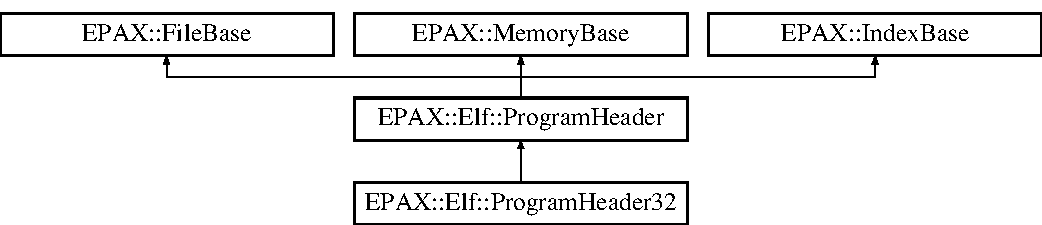
\includegraphics[height=3.000000cm]{class_e_p_a_x_1_1_elf_1_1_program_header32}
\end{center}
\end{figure}
\subsection*{\-Public \-Member \-Functions}
\begin{DoxyCompactItemize}
\item 
\hyperlink{class_e_p_a_x_1_1_elf_1_1_program_header32_a989edb2ff17c082517e51416331c1904}{\-Program\-Header32} (\hyperlink{class_e_p_a_x_1_1_base_binary}{\-Base\-Binary} $\ast$b, uint64\-\_\-t o, uint64\-\_\-t s, uint32\-\_\-t i)
\item 
virtual \hyperlink{class_e_p_a_x_1_1_elf_1_1_program_header32_a6ecc03af8b1082a3c39432d979c77aa0}{$\sim$\-Program\-Header32} ()
\item 
uint64\-\_\-t \hyperlink{class_e_p_a_x_1_1_elf_1_1_program_header32_a66eba7a23760b1a7955dc3821163a67e}{get\-Vaddr} ()
\item 
uint64\-\_\-t \hyperlink{class_e_p_a_x_1_1_elf_1_1_program_header32_a00042a0b2d817185d053d0647956261f}{get\-Paddr} ()
\item 
uint64\-\_\-t \hyperlink{class_e_p_a_x_1_1_elf_1_1_program_header32_a8eac270d2eff779a2f7de736f0b77113}{get\-F\-Size} ()
\item 
uint64\-\_\-t \hyperlink{class_e_p_a_x_1_1_elf_1_1_program_header32_a81d8e54c74130cc27f72ceb27a2044af}{get\-M\-Size} ()
\item 
uint32\-\_\-t \hyperlink{class_e_p_a_x_1_1_elf_1_1_program_header32_af00964314bdbe0342ea9ef1ff2a156ab}{get\-Segment\-Type} ()
\item 
uint64\-\_\-t \hyperlink{class_e_p_a_x_1_1_elf_1_1_program_header32_ac97782a148e1eacf90b38720e535cbef}{get\-Flags} ()
\item 
uint32\-\_\-t \hyperlink{class_e_p_a_x_1_1_elf_1_1_program_header32_a8b50e70db41f7b4f646f1ab2b54c227a}{get\-Alignment} ()
\item 
uint64\-\_\-t \hyperlink{class_e_p_a_x_1_1_elf_1_1_program_header32_a46bdc77ad9a585e058f0dadcc4e71831}{get\-F\-Offset} ()
\end{DoxyCompactItemize}


\subsection{\-Detailed \-Description}


\-Definition at line 340 of file \-Elf\-Binary.\-hpp.



\subsection{\-Constructor \& \-Destructor \-Documentation}
\hypertarget{class_e_p_a_x_1_1_elf_1_1_program_header32_a989edb2ff17c082517e51416331c1904}{\index{\-E\-P\-A\-X\-::\-Elf\-::\-Program\-Header32@{\-E\-P\-A\-X\-::\-Elf\-::\-Program\-Header32}!\-Program\-Header32@{\-Program\-Header32}}
\index{\-Program\-Header32@{\-Program\-Header32}!EPAX::Elf::ProgramHeader32@{\-E\-P\-A\-X\-::\-Elf\-::\-Program\-Header32}}
\subsubsection[{\-Program\-Header32}]{\setlength{\rightskip}{0pt plus 5cm}{\bf \-E\-P\-A\-X\-::\-Elf\-::\-Program\-Header32\-::\-Program\-Header32} (
\begin{DoxyParamCaption}
\item[{{\bf \-Base\-Binary} $\ast$}]{b, }
\item[{uint64\-\_\-t}]{o, }
\item[{uint64\-\_\-t}]{s, }
\item[{uint32\-\_\-t}]{i}
\end{DoxyParamCaption}
)}}\label{class_e_p_a_x_1_1_elf_1_1_program_header32_a989edb2ff17c082517e51416331c1904}


\-Definition at line 884 of file \-Elf\-Binary.\-cpp.

\hypertarget{class_e_p_a_x_1_1_elf_1_1_program_header32_a6ecc03af8b1082a3c39432d979c77aa0}{\index{\-E\-P\-A\-X\-::\-Elf\-::\-Program\-Header32@{\-E\-P\-A\-X\-::\-Elf\-::\-Program\-Header32}!$\sim$\-Program\-Header32@{$\sim$\-Program\-Header32}}
\index{$\sim$\-Program\-Header32@{$\sim$\-Program\-Header32}!EPAX::Elf::ProgramHeader32@{\-E\-P\-A\-X\-::\-Elf\-::\-Program\-Header32}}
\subsubsection[{$\sim$\-Program\-Header32}]{\setlength{\rightskip}{0pt plus 5cm}virtual {\bf \-E\-P\-A\-X\-::\-Elf\-::\-Program\-Header32\-::$\sim$\-Program\-Header32} (
\begin{DoxyParamCaption}
{}
\end{DoxyParamCaption}
)\hspace{0.3cm}{\ttfamily  \mbox{[}inline, virtual\mbox{]}}}}\label{class_e_p_a_x_1_1_elf_1_1_program_header32_a6ecc03af8b1082a3c39432d979c77aa0}


\-Definition at line 343 of file \-Elf\-Binary.\-hpp.



\subsection{\-Member \-Function \-Documentation}
\hypertarget{class_e_p_a_x_1_1_elf_1_1_program_header32_a8b50e70db41f7b4f646f1ab2b54c227a}{\index{\-E\-P\-A\-X\-::\-Elf\-::\-Program\-Header32@{\-E\-P\-A\-X\-::\-Elf\-::\-Program\-Header32}!get\-Alignment@{get\-Alignment}}
\index{get\-Alignment@{get\-Alignment}!EPAX::Elf::ProgramHeader32@{\-E\-P\-A\-X\-::\-Elf\-::\-Program\-Header32}}
\subsubsection[{get\-Alignment}]{\setlength{\rightskip}{0pt plus 5cm}uint32\-\_\-t {\bf \-E\-P\-A\-X\-::\-Elf\-::\-Program\-Header32\-::get\-Alignment} (
\begin{DoxyParamCaption}
{}
\end{DoxyParamCaption}
)\hspace{0.3cm}{\ttfamily  \mbox{[}virtual\mbox{]}}}}\label{class_e_p_a_x_1_1_elf_1_1_program_header32_a8b50e70db41f7b4f646f1ab2b54c227a}


\-Implements \hyperlink{class_e_p_a_x_1_1_elf_1_1_program_header_acfef642e82022bdd883944e48dff4015}{\-E\-P\-A\-X\-::\-Elf\-::\-Program\-Header}.



\-Definition at line 938 of file \-Elf\-Binary.\-cpp.

\hypertarget{class_e_p_a_x_1_1_elf_1_1_program_header32_ac97782a148e1eacf90b38720e535cbef}{\index{\-E\-P\-A\-X\-::\-Elf\-::\-Program\-Header32@{\-E\-P\-A\-X\-::\-Elf\-::\-Program\-Header32}!get\-Flags@{get\-Flags}}
\index{get\-Flags@{get\-Flags}!EPAX::Elf::ProgramHeader32@{\-E\-P\-A\-X\-::\-Elf\-::\-Program\-Header32}}
\subsubsection[{get\-Flags}]{\setlength{\rightskip}{0pt plus 5cm}uint64\-\_\-t {\bf \-E\-P\-A\-X\-::\-Elf\-::\-Program\-Header32\-::get\-Flags} (
\begin{DoxyParamCaption}
{}
\end{DoxyParamCaption}
)\hspace{0.3cm}{\ttfamily  \mbox{[}virtual\mbox{]}}}}\label{class_e_p_a_x_1_1_elf_1_1_program_header32_ac97782a148e1eacf90b38720e535cbef}


\-Implements \hyperlink{class_e_p_a_x_1_1_elf_1_1_program_header_a566bcceecb66e2b159e3e52b44e2f941}{\-E\-P\-A\-X\-::\-Elf\-::\-Program\-Header}.



\-Definition at line 930 of file \-Elf\-Binary.\-cpp.

\hypertarget{class_e_p_a_x_1_1_elf_1_1_program_header32_a46bdc77ad9a585e058f0dadcc4e71831}{\index{\-E\-P\-A\-X\-::\-Elf\-::\-Program\-Header32@{\-E\-P\-A\-X\-::\-Elf\-::\-Program\-Header32}!get\-F\-Offset@{get\-F\-Offset}}
\index{get\-F\-Offset@{get\-F\-Offset}!EPAX::Elf::ProgramHeader32@{\-E\-P\-A\-X\-::\-Elf\-::\-Program\-Header32}}
\subsubsection[{get\-F\-Offset}]{\setlength{\rightskip}{0pt plus 5cm}uint64\-\_\-t {\bf \-E\-P\-A\-X\-::\-Elf\-::\-Program\-Header32\-::get\-F\-Offset} (
\begin{DoxyParamCaption}
{}
\end{DoxyParamCaption}
)\hspace{0.3cm}{\ttfamily  \mbox{[}virtual\mbox{]}}}}\label{class_e_p_a_x_1_1_elf_1_1_program_header32_a46bdc77ad9a585e058f0dadcc4e71831}


\-Implements \hyperlink{class_e_p_a_x_1_1_elf_1_1_program_header_a328166b748f2717c9da393210f7aa9cc}{\-E\-P\-A\-X\-::\-Elf\-::\-Program\-Header}.



\-Definition at line 954 of file \-Elf\-Binary.\-cpp.

\hypertarget{class_e_p_a_x_1_1_elf_1_1_program_header32_a8eac270d2eff779a2f7de736f0b77113}{\index{\-E\-P\-A\-X\-::\-Elf\-::\-Program\-Header32@{\-E\-P\-A\-X\-::\-Elf\-::\-Program\-Header32}!get\-F\-Size@{get\-F\-Size}}
\index{get\-F\-Size@{get\-F\-Size}!EPAX::Elf::ProgramHeader32@{\-E\-P\-A\-X\-::\-Elf\-::\-Program\-Header32}}
\subsubsection[{get\-F\-Size}]{\setlength{\rightskip}{0pt plus 5cm}uint64\-\_\-t {\bf \-E\-P\-A\-X\-::\-Elf\-::\-Program\-Header32\-::get\-F\-Size} (
\begin{DoxyParamCaption}
{}
\end{DoxyParamCaption}
)\hspace{0.3cm}{\ttfamily  \mbox{[}virtual\mbox{]}}}}\label{class_e_p_a_x_1_1_elf_1_1_program_header32_a8eac270d2eff779a2f7de736f0b77113}


\-Implements \hyperlink{class_e_p_a_x_1_1_elf_1_1_program_header_aa0dfb27d2bb6b869c2810c2ee070ff7b}{\-E\-P\-A\-X\-::\-Elf\-::\-Program\-Header}.



\-Definition at line 914 of file \-Elf\-Binary.\-cpp.

\hypertarget{class_e_p_a_x_1_1_elf_1_1_program_header32_a81d8e54c74130cc27f72ceb27a2044af}{\index{\-E\-P\-A\-X\-::\-Elf\-::\-Program\-Header32@{\-E\-P\-A\-X\-::\-Elf\-::\-Program\-Header32}!get\-M\-Size@{get\-M\-Size}}
\index{get\-M\-Size@{get\-M\-Size}!EPAX::Elf::ProgramHeader32@{\-E\-P\-A\-X\-::\-Elf\-::\-Program\-Header32}}
\subsubsection[{get\-M\-Size}]{\setlength{\rightskip}{0pt plus 5cm}uint64\-\_\-t {\bf \-E\-P\-A\-X\-::\-Elf\-::\-Program\-Header32\-::get\-M\-Size} (
\begin{DoxyParamCaption}
{}
\end{DoxyParamCaption}
)\hspace{0.3cm}{\ttfamily  \mbox{[}virtual\mbox{]}}}}\label{class_e_p_a_x_1_1_elf_1_1_program_header32_a81d8e54c74130cc27f72ceb27a2044af}


\-Implements \hyperlink{class_e_p_a_x_1_1_elf_1_1_program_header_ab624186a1963231b21722025d9f87a32}{\-E\-P\-A\-X\-::\-Elf\-::\-Program\-Header}.



\-Definition at line 922 of file \-Elf\-Binary.\-cpp.

\hypertarget{class_e_p_a_x_1_1_elf_1_1_program_header32_a00042a0b2d817185d053d0647956261f}{\index{\-E\-P\-A\-X\-::\-Elf\-::\-Program\-Header32@{\-E\-P\-A\-X\-::\-Elf\-::\-Program\-Header32}!get\-Paddr@{get\-Paddr}}
\index{get\-Paddr@{get\-Paddr}!EPAX::Elf::ProgramHeader32@{\-E\-P\-A\-X\-::\-Elf\-::\-Program\-Header32}}
\subsubsection[{get\-Paddr}]{\setlength{\rightskip}{0pt plus 5cm}uint64\-\_\-t {\bf \-E\-P\-A\-X\-::\-Elf\-::\-Program\-Header32\-::get\-Paddr} (
\begin{DoxyParamCaption}
{}
\end{DoxyParamCaption}
)\hspace{0.3cm}{\ttfamily  \mbox{[}virtual\mbox{]}}}}\label{class_e_p_a_x_1_1_elf_1_1_program_header32_a00042a0b2d817185d053d0647956261f}


\-Implements \hyperlink{class_e_p_a_x_1_1_elf_1_1_program_header_aff0f58569378cdcb6c4d7ab309af62c7}{\-E\-P\-A\-X\-::\-Elf\-::\-Program\-Header}.



\-Definition at line 906 of file \-Elf\-Binary.\-cpp.

\hypertarget{class_e_p_a_x_1_1_elf_1_1_program_header32_af00964314bdbe0342ea9ef1ff2a156ab}{\index{\-E\-P\-A\-X\-::\-Elf\-::\-Program\-Header32@{\-E\-P\-A\-X\-::\-Elf\-::\-Program\-Header32}!get\-Segment\-Type@{get\-Segment\-Type}}
\index{get\-Segment\-Type@{get\-Segment\-Type}!EPAX::Elf::ProgramHeader32@{\-E\-P\-A\-X\-::\-Elf\-::\-Program\-Header32}}
\subsubsection[{get\-Segment\-Type}]{\setlength{\rightskip}{0pt plus 5cm}uint32\-\_\-t {\bf \-E\-P\-A\-X\-::\-Elf\-::\-Program\-Header32\-::get\-Segment\-Type} (
\begin{DoxyParamCaption}
{}
\end{DoxyParamCaption}
)\hspace{0.3cm}{\ttfamily  \mbox{[}virtual\mbox{]}}}}\label{class_e_p_a_x_1_1_elf_1_1_program_header32_af00964314bdbe0342ea9ef1ff2a156ab}


\-Implements \hyperlink{class_e_p_a_x_1_1_elf_1_1_program_header_a2034c6e8212ac3ced6719a706b48d6d1}{\-E\-P\-A\-X\-::\-Elf\-::\-Program\-Header}.



\-Definition at line 946 of file \-Elf\-Binary.\-cpp.

\hypertarget{class_e_p_a_x_1_1_elf_1_1_program_header32_a66eba7a23760b1a7955dc3821163a67e}{\index{\-E\-P\-A\-X\-::\-Elf\-::\-Program\-Header32@{\-E\-P\-A\-X\-::\-Elf\-::\-Program\-Header32}!get\-Vaddr@{get\-Vaddr}}
\index{get\-Vaddr@{get\-Vaddr}!EPAX::Elf::ProgramHeader32@{\-E\-P\-A\-X\-::\-Elf\-::\-Program\-Header32}}
\subsubsection[{get\-Vaddr}]{\setlength{\rightskip}{0pt plus 5cm}uint64\-\_\-t {\bf \-E\-P\-A\-X\-::\-Elf\-::\-Program\-Header32\-::get\-Vaddr} (
\begin{DoxyParamCaption}
{}
\end{DoxyParamCaption}
)\hspace{0.3cm}{\ttfamily  \mbox{[}virtual\mbox{]}}}}\label{class_e_p_a_x_1_1_elf_1_1_program_header32_a66eba7a23760b1a7955dc3821163a67e}


\-Implements \hyperlink{class_e_p_a_x_1_1_elf_1_1_program_header_aa8a7d552ece248bccfda3d320fe2d2ab}{\-E\-P\-A\-X\-::\-Elf\-::\-Program\-Header}.



\-Definition at line 898 of file \-Elf\-Binary.\-cpp.



\-The documentation for this class was generated from the following files\-:\begin{DoxyCompactItemize}
\item 
\hyperlink{_elf_binary_8hpp}{\-Elf\-Binary.\-hpp}\item 
\hyperlink{_elf_binary_8cpp}{\-Elf\-Binary.\-cpp}\end{DoxyCompactItemize}

\hypertarget{class_e_p_a_x_1_1_elf_1_1_program_header64}{\section{\-E\-P\-A\-X\-:\-:\-Elf\-:\-:\-Program\-Header64 \-Class \-Reference}
\label{class_e_p_a_x_1_1_elf_1_1_program_header64}\index{\-E\-P\-A\-X\-::\-Elf\-::\-Program\-Header64@{\-E\-P\-A\-X\-::\-Elf\-::\-Program\-Header64}}
}


{\ttfamily \#include $<$\-Elf\-Binary.\-hpp$>$}

\-Inheritance diagram for \-E\-P\-A\-X\-:\-:\-Elf\-:\-:\-Program\-Header64\-:\begin{figure}[H]
\begin{center}
\leavevmode
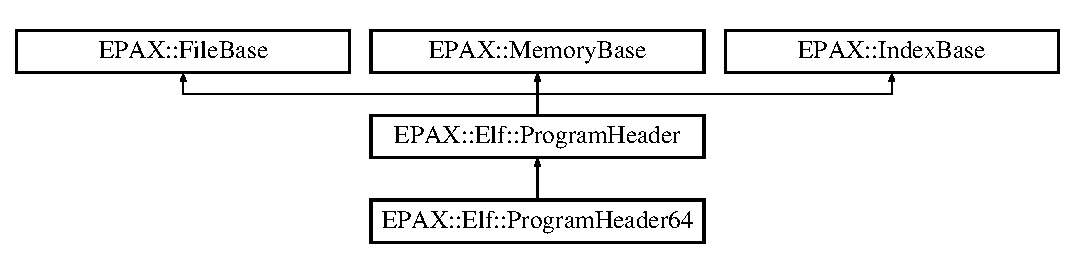
\includegraphics[height=3.000000cm]{class_e_p_a_x_1_1_elf_1_1_program_header64}
\end{center}
\end{figure}
\subsection*{\-Public \-Member \-Functions}
\begin{DoxyCompactItemize}
\item 
\hyperlink{class_e_p_a_x_1_1_elf_1_1_program_header64_aa65ae437cdc94378ed92b3a843325d3e}{\-Program\-Header64} (\hyperlink{class_e_p_a_x_1_1_base_binary}{\-Base\-Binary} $\ast$b, uint64\-\_\-t o, uint64\-\_\-t s, uint32\-\_\-t i)
\item 
virtual \hyperlink{class_e_p_a_x_1_1_elf_1_1_program_header64_a0f4239d70bbccd023c1861f0c3e55b2b}{$\sim$\-Program\-Header64} ()
\item 
uint64\-\_\-t \hyperlink{class_e_p_a_x_1_1_elf_1_1_program_header64_a3b8ed64a54eb47450dff7be0ee28817b}{get\-Vaddr} ()
\item 
uint64\-\_\-t \hyperlink{class_e_p_a_x_1_1_elf_1_1_program_header64_a7e1bc27b844418b80f56c458a49797a6}{get\-Paddr} ()
\item 
uint64\-\_\-t \hyperlink{class_e_p_a_x_1_1_elf_1_1_program_header64_a04e7b5890ccc7c01d23e221fbfc44708}{get\-F\-Size} ()
\item 
uint64\-\_\-t \hyperlink{class_e_p_a_x_1_1_elf_1_1_program_header64_a821b37a8d6ebdf7fea555e7a4434eac2}{get\-M\-Size} ()
\item 
uint32\-\_\-t \hyperlink{class_e_p_a_x_1_1_elf_1_1_program_header64_a5a35087dbe63d5fdabd5893bb57c38a3}{get\-Segment\-Type} ()
\item 
uint64\-\_\-t \hyperlink{class_e_p_a_x_1_1_elf_1_1_program_header64_a9f12ad0de269ad3c5c7f2fc52f72fc5a}{get\-Flags} ()
\item 
uint32\-\_\-t \hyperlink{class_e_p_a_x_1_1_elf_1_1_program_header64_a68a761d44891ce538049b04236fe2a9c}{get\-Alignment} ()
\item 
uint64\-\_\-t \hyperlink{class_e_p_a_x_1_1_elf_1_1_program_header64_adde9f4fb75d093fcc7f30d42909f8ef5}{get\-F\-Offset} ()
\end{DoxyCompactItemize}


\subsection{\-Detailed \-Description}


\-Definition at line 355 of file \-Elf\-Binary.\-hpp.



\subsection{\-Constructor \& \-Destructor \-Documentation}
\hypertarget{class_e_p_a_x_1_1_elf_1_1_program_header64_aa65ae437cdc94378ed92b3a843325d3e}{\index{\-E\-P\-A\-X\-::\-Elf\-::\-Program\-Header64@{\-E\-P\-A\-X\-::\-Elf\-::\-Program\-Header64}!\-Program\-Header64@{\-Program\-Header64}}
\index{\-Program\-Header64@{\-Program\-Header64}!EPAX::Elf::ProgramHeader64@{\-E\-P\-A\-X\-::\-Elf\-::\-Program\-Header64}}
\subsubsection[{\-Program\-Header64}]{\setlength{\rightskip}{0pt plus 5cm}{\bf \-E\-P\-A\-X\-::\-Elf\-::\-Program\-Header64\-::\-Program\-Header64} (
\begin{DoxyParamCaption}
\item[{{\bf \-Base\-Binary} $\ast$}]{b, }
\item[{uint64\-\_\-t}]{o, }
\item[{uint64\-\_\-t}]{s, }
\item[{uint32\-\_\-t}]{i}
\end{DoxyParamCaption}
)}}\label{class_e_p_a_x_1_1_elf_1_1_program_header64_aa65ae437cdc94378ed92b3a843325d3e}


\-Definition at line 891 of file \-Elf\-Binary.\-cpp.

\hypertarget{class_e_p_a_x_1_1_elf_1_1_program_header64_a0f4239d70bbccd023c1861f0c3e55b2b}{\index{\-E\-P\-A\-X\-::\-Elf\-::\-Program\-Header64@{\-E\-P\-A\-X\-::\-Elf\-::\-Program\-Header64}!$\sim$\-Program\-Header64@{$\sim$\-Program\-Header64}}
\index{$\sim$\-Program\-Header64@{$\sim$\-Program\-Header64}!EPAX::Elf::ProgramHeader64@{\-E\-P\-A\-X\-::\-Elf\-::\-Program\-Header64}}
\subsubsection[{$\sim$\-Program\-Header64}]{\setlength{\rightskip}{0pt plus 5cm}virtual {\bf \-E\-P\-A\-X\-::\-Elf\-::\-Program\-Header64\-::$\sim$\-Program\-Header64} (
\begin{DoxyParamCaption}
{}
\end{DoxyParamCaption}
)\hspace{0.3cm}{\ttfamily  \mbox{[}inline, virtual\mbox{]}}}}\label{class_e_p_a_x_1_1_elf_1_1_program_header64_a0f4239d70bbccd023c1861f0c3e55b2b}


\-Definition at line 358 of file \-Elf\-Binary.\-hpp.



\subsection{\-Member \-Function \-Documentation}
\hypertarget{class_e_p_a_x_1_1_elf_1_1_program_header64_a68a761d44891ce538049b04236fe2a9c}{\index{\-E\-P\-A\-X\-::\-Elf\-::\-Program\-Header64@{\-E\-P\-A\-X\-::\-Elf\-::\-Program\-Header64}!get\-Alignment@{get\-Alignment}}
\index{get\-Alignment@{get\-Alignment}!EPAX::Elf::ProgramHeader64@{\-E\-P\-A\-X\-::\-Elf\-::\-Program\-Header64}}
\subsubsection[{get\-Alignment}]{\setlength{\rightskip}{0pt plus 5cm}uint32\-\_\-t {\bf \-E\-P\-A\-X\-::\-Elf\-::\-Program\-Header64\-::get\-Alignment} (
\begin{DoxyParamCaption}
{}
\end{DoxyParamCaption}
)\hspace{0.3cm}{\ttfamily  \mbox{[}virtual\mbox{]}}}}\label{class_e_p_a_x_1_1_elf_1_1_program_header64_a68a761d44891ce538049b04236fe2a9c}


\-Implements \hyperlink{class_e_p_a_x_1_1_elf_1_1_program_header_acfef642e82022bdd883944e48dff4015}{\-E\-P\-A\-X\-::\-Elf\-::\-Program\-Header}.



\-Definition at line 942 of file \-Elf\-Binary.\-cpp.

\hypertarget{class_e_p_a_x_1_1_elf_1_1_program_header64_a9f12ad0de269ad3c5c7f2fc52f72fc5a}{\index{\-E\-P\-A\-X\-::\-Elf\-::\-Program\-Header64@{\-E\-P\-A\-X\-::\-Elf\-::\-Program\-Header64}!get\-Flags@{get\-Flags}}
\index{get\-Flags@{get\-Flags}!EPAX::Elf::ProgramHeader64@{\-E\-P\-A\-X\-::\-Elf\-::\-Program\-Header64}}
\subsubsection[{get\-Flags}]{\setlength{\rightskip}{0pt plus 5cm}uint64\-\_\-t {\bf \-E\-P\-A\-X\-::\-Elf\-::\-Program\-Header64\-::get\-Flags} (
\begin{DoxyParamCaption}
{}
\end{DoxyParamCaption}
)\hspace{0.3cm}{\ttfamily  \mbox{[}virtual\mbox{]}}}}\label{class_e_p_a_x_1_1_elf_1_1_program_header64_a9f12ad0de269ad3c5c7f2fc52f72fc5a}


\-Implements \hyperlink{class_e_p_a_x_1_1_elf_1_1_program_header_a566bcceecb66e2b159e3e52b44e2f941}{\-E\-P\-A\-X\-::\-Elf\-::\-Program\-Header}.



\-Definition at line 934 of file \-Elf\-Binary.\-cpp.

\hypertarget{class_e_p_a_x_1_1_elf_1_1_program_header64_adde9f4fb75d093fcc7f30d42909f8ef5}{\index{\-E\-P\-A\-X\-::\-Elf\-::\-Program\-Header64@{\-E\-P\-A\-X\-::\-Elf\-::\-Program\-Header64}!get\-F\-Offset@{get\-F\-Offset}}
\index{get\-F\-Offset@{get\-F\-Offset}!EPAX::Elf::ProgramHeader64@{\-E\-P\-A\-X\-::\-Elf\-::\-Program\-Header64}}
\subsubsection[{get\-F\-Offset}]{\setlength{\rightskip}{0pt plus 5cm}uint64\-\_\-t {\bf \-E\-P\-A\-X\-::\-Elf\-::\-Program\-Header64\-::get\-F\-Offset} (
\begin{DoxyParamCaption}
{}
\end{DoxyParamCaption}
)\hspace{0.3cm}{\ttfamily  \mbox{[}virtual\mbox{]}}}}\label{class_e_p_a_x_1_1_elf_1_1_program_header64_adde9f4fb75d093fcc7f30d42909f8ef5}


\-Implements \hyperlink{class_e_p_a_x_1_1_elf_1_1_program_header_a328166b748f2717c9da393210f7aa9cc}{\-E\-P\-A\-X\-::\-Elf\-::\-Program\-Header}.



\-Definition at line 958 of file \-Elf\-Binary.\-cpp.

\hypertarget{class_e_p_a_x_1_1_elf_1_1_program_header64_a04e7b5890ccc7c01d23e221fbfc44708}{\index{\-E\-P\-A\-X\-::\-Elf\-::\-Program\-Header64@{\-E\-P\-A\-X\-::\-Elf\-::\-Program\-Header64}!get\-F\-Size@{get\-F\-Size}}
\index{get\-F\-Size@{get\-F\-Size}!EPAX::Elf::ProgramHeader64@{\-E\-P\-A\-X\-::\-Elf\-::\-Program\-Header64}}
\subsubsection[{get\-F\-Size}]{\setlength{\rightskip}{0pt plus 5cm}uint64\-\_\-t {\bf \-E\-P\-A\-X\-::\-Elf\-::\-Program\-Header64\-::get\-F\-Size} (
\begin{DoxyParamCaption}
{}
\end{DoxyParamCaption}
)\hspace{0.3cm}{\ttfamily  \mbox{[}virtual\mbox{]}}}}\label{class_e_p_a_x_1_1_elf_1_1_program_header64_a04e7b5890ccc7c01d23e221fbfc44708}


\-Implements \hyperlink{class_e_p_a_x_1_1_elf_1_1_program_header_aa0dfb27d2bb6b869c2810c2ee070ff7b}{\-E\-P\-A\-X\-::\-Elf\-::\-Program\-Header}.



\-Definition at line 918 of file \-Elf\-Binary.\-cpp.

\hypertarget{class_e_p_a_x_1_1_elf_1_1_program_header64_a821b37a8d6ebdf7fea555e7a4434eac2}{\index{\-E\-P\-A\-X\-::\-Elf\-::\-Program\-Header64@{\-E\-P\-A\-X\-::\-Elf\-::\-Program\-Header64}!get\-M\-Size@{get\-M\-Size}}
\index{get\-M\-Size@{get\-M\-Size}!EPAX::Elf::ProgramHeader64@{\-E\-P\-A\-X\-::\-Elf\-::\-Program\-Header64}}
\subsubsection[{get\-M\-Size}]{\setlength{\rightskip}{0pt plus 5cm}uint64\-\_\-t {\bf \-E\-P\-A\-X\-::\-Elf\-::\-Program\-Header64\-::get\-M\-Size} (
\begin{DoxyParamCaption}
{}
\end{DoxyParamCaption}
)\hspace{0.3cm}{\ttfamily  \mbox{[}virtual\mbox{]}}}}\label{class_e_p_a_x_1_1_elf_1_1_program_header64_a821b37a8d6ebdf7fea555e7a4434eac2}


\-Implements \hyperlink{class_e_p_a_x_1_1_elf_1_1_program_header_ab624186a1963231b21722025d9f87a32}{\-E\-P\-A\-X\-::\-Elf\-::\-Program\-Header}.



\-Definition at line 926 of file \-Elf\-Binary.\-cpp.

\hypertarget{class_e_p_a_x_1_1_elf_1_1_program_header64_a7e1bc27b844418b80f56c458a49797a6}{\index{\-E\-P\-A\-X\-::\-Elf\-::\-Program\-Header64@{\-E\-P\-A\-X\-::\-Elf\-::\-Program\-Header64}!get\-Paddr@{get\-Paddr}}
\index{get\-Paddr@{get\-Paddr}!EPAX::Elf::ProgramHeader64@{\-E\-P\-A\-X\-::\-Elf\-::\-Program\-Header64}}
\subsubsection[{get\-Paddr}]{\setlength{\rightskip}{0pt plus 5cm}uint64\-\_\-t {\bf \-E\-P\-A\-X\-::\-Elf\-::\-Program\-Header64\-::get\-Paddr} (
\begin{DoxyParamCaption}
{}
\end{DoxyParamCaption}
)\hspace{0.3cm}{\ttfamily  \mbox{[}virtual\mbox{]}}}}\label{class_e_p_a_x_1_1_elf_1_1_program_header64_a7e1bc27b844418b80f56c458a49797a6}


\-Implements \hyperlink{class_e_p_a_x_1_1_elf_1_1_program_header_aff0f58569378cdcb6c4d7ab309af62c7}{\-E\-P\-A\-X\-::\-Elf\-::\-Program\-Header}.



\-Definition at line 910 of file \-Elf\-Binary.\-cpp.

\hypertarget{class_e_p_a_x_1_1_elf_1_1_program_header64_a5a35087dbe63d5fdabd5893bb57c38a3}{\index{\-E\-P\-A\-X\-::\-Elf\-::\-Program\-Header64@{\-E\-P\-A\-X\-::\-Elf\-::\-Program\-Header64}!get\-Segment\-Type@{get\-Segment\-Type}}
\index{get\-Segment\-Type@{get\-Segment\-Type}!EPAX::Elf::ProgramHeader64@{\-E\-P\-A\-X\-::\-Elf\-::\-Program\-Header64}}
\subsubsection[{get\-Segment\-Type}]{\setlength{\rightskip}{0pt plus 5cm}uint32\-\_\-t {\bf \-E\-P\-A\-X\-::\-Elf\-::\-Program\-Header64\-::get\-Segment\-Type} (
\begin{DoxyParamCaption}
{}
\end{DoxyParamCaption}
)\hspace{0.3cm}{\ttfamily  \mbox{[}virtual\mbox{]}}}}\label{class_e_p_a_x_1_1_elf_1_1_program_header64_a5a35087dbe63d5fdabd5893bb57c38a3}


\-Implements \hyperlink{class_e_p_a_x_1_1_elf_1_1_program_header_a2034c6e8212ac3ced6719a706b48d6d1}{\-E\-P\-A\-X\-::\-Elf\-::\-Program\-Header}.



\-Definition at line 950 of file \-Elf\-Binary.\-cpp.

\hypertarget{class_e_p_a_x_1_1_elf_1_1_program_header64_a3b8ed64a54eb47450dff7be0ee28817b}{\index{\-E\-P\-A\-X\-::\-Elf\-::\-Program\-Header64@{\-E\-P\-A\-X\-::\-Elf\-::\-Program\-Header64}!get\-Vaddr@{get\-Vaddr}}
\index{get\-Vaddr@{get\-Vaddr}!EPAX::Elf::ProgramHeader64@{\-E\-P\-A\-X\-::\-Elf\-::\-Program\-Header64}}
\subsubsection[{get\-Vaddr}]{\setlength{\rightskip}{0pt plus 5cm}uint64\-\_\-t {\bf \-E\-P\-A\-X\-::\-Elf\-::\-Program\-Header64\-::get\-Vaddr} (
\begin{DoxyParamCaption}
{}
\end{DoxyParamCaption}
)\hspace{0.3cm}{\ttfamily  \mbox{[}virtual\mbox{]}}}}\label{class_e_p_a_x_1_1_elf_1_1_program_header64_a3b8ed64a54eb47450dff7be0ee28817b}


\-Implements \hyperlink{class_e_p_a_x_1_1_elf_1_1_program_header_aa8a7d552ece248bccfda3d320fe2d2ab}{\-E\-P\-A\-X\-::\-Elf\-::\-Program\-Header}.



\-Definition at line 902 of file \-Elf\-Binary.\-cpp.



\-The documentation for this class was generated from the following files\-:\begin{DoxyCompactItemize}
\item 
\hyperlink{_elf_binary_8hpp}{\-Elf\-Binary.\-hpp}\item 
\hyperlink{_elf_binary_8cpp}{\-Elf\-Binary.\-cpp}\end{DoxyCompactItemize}

\hypertarget{class_e_p_a_x_1_1_section}{\section{\-E\-P\-A\-X\-:\-:\-Section \-Class \-Reference}
\label{class_e_p_a_x_1_1_section}\index{\-E\-P\-A\-X\-::\-Section@{\-E\-P\-A\-X\-::\-Section}}
}


{\ttfamily \#include $<$\-Section.\-hpp$>$}

\-Inheritance diagram for \-E\-P\-A\-X\-:\-:\-Section\-:\begin{figure}[H]
\begin{center}
\leavevmode
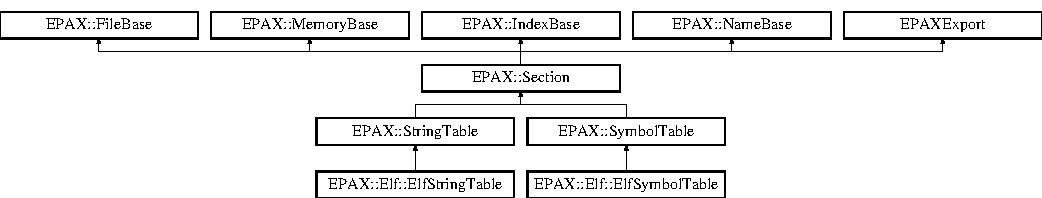
\includegraphics[height=2.666667cm]{class_e_p_a_x_1_1_section}
\end{center}
\end{figure}
\subsection*{\-Public \-Member \-Functions}
\begin{DoxyCompactItemize}
\item 
\hyperlink{class_e_p_a_x_1_1_section_a90d6591d88f81dadbc86b93a53954eee}{\-Section} (\hyperlink{class_e_p_a_x_1_1_base_binary}{\-Base\-Binary} $\ast$b, uint64\-\_\-t o, uint64\-\_\-t fs, uint64\-\_\-t ma, uint64\-\_\-t ms, uint32\-\_\-t i, std\-::string n)
\item 
virtual \hyperlink{class_e_p_a_x_1_1_section_ad7eeb2596e6e8070b0ffa495c849c214}{$\sim$\-Section} ()
\item 
virtual void \hyperlink{class_e_p_a_x_1_1_section_ad79a91be22efd4499b78d2554ebc8285}{print} (std\-::ostream \&stream=std\-::cout)
\item 
virtual bool \hyperlink{class_e_p_a_x_1_1_section_a368308eb714d2e274ac82c1a92824b28}{is\-Text} ()
\item 
virtual bool \hyperlink{class_e_p_a_x_1_1_section_a90db97c9ef10f64fad4a339a2c3b128c}{is\-Data} ()
\item 
virtual bool \hyperlink{class_e_p_a_x_1_1_section_a0518a2160f8bd57836b8f9823993376c}{is\-B\-S\-S} ()
\item 
virtual bool \hyperlink{class_e_p_a_x_1_1_section_a43c6a0b55e15f24689838084c97cffe8}{is\-Debug} ()
\item 
virtual bool \hyperlink{class_e_p_a_x_1_1_section_a04c811caf98179122fa6443095bde52d}{is\-String} ()
\item 
virtual bool \hyperlink{class_e_p_a_x_1_1_section_a6f8fdba06c4f3506d4dc2df97658157f}{is\-Symbol} ()
\end{DoxyCompactItemize}


\subsection{\-Detailed \-Description}


\-Definition at line 35 of file \-Section.\-hpp.



\subsection{\-Constructor \& \-Destructor \-Documentation}
\hypertarget{class_e_p_a_x_1_1_section_a90d6591d88f81dadbc86b93a53954eee}{\index{\-E\-P\-A\-X\-::\-Section@{\-E\-P\-A\-X\-::\-Section}!\-Section@{\-Section}}
\index{\-Section@{\-Section}!EPAX::Section@{\-E\-P\-A\-X\-::\-Section}}
\subsubsection[{\-Section}]{\setlength{\rightskip}{0pt plus 5cm}{\bf \-E\-P\-A\-X\-::\-Section\-::\-Section} (
\begin{DoxyParamCaption}
\item[{{\bf \-Base\-Binary} $\ast$}]{b, }
\item[{uint64\-\_\-t}]{o, }
\item[{uint64\-\_\-t}]{fs, }
\item[{uint64\-\_\-t}]{ma, }
\item[{uint64\-\_\-t}]{ms, }
\item[{uint32\-\_\-t}]{i, }
\item[{std\-::string}]{n}
\end{DoxyParamCaption}
)}}\label{class_e_p_a_x_1_1_section_a90d6591d88f81dadbc86b93a53954eee}


\-Definition at line 31 of file \-Section.\-cpp.

\hypertarget{class_e_p_a_x_1_1_section_ad7eeb2596e6e8070b0ffa495c849c214}{\index{\-E\-P\-A\-X\-::\-Section@{\-E\-P\-A\-X\-::\-Section}!$\sim$\-Section@{$\sim$\-Section}}
\index{$\sim$\-Section@{$\sim$\-Section}!EPAX::Section@{\-E\-P\-A\-X\-::\-Section}}
\subsubsection[{$\sim$\-Section}]{\setlength{\rightskip}{0pt plus 5cm}virtual {\bf \-E\-P\-A\-X\-::\-Section\-::$\sim$\-Section} (
\begin{DoxyParamCaption}
{}
\end{DoxyParamCaption}
)\hspace{0.3cm}{\ttfamily  \mbox{[}inline, virtual\mbox{]}}}}\label{class_e_p_a_x_1_1_section_ad7eeb2596e6e8070b0ffa495c849c214}


\-Definition at line 38 of file \-Section.\-hpp.



\subsection{\-Member \-Function \-Documentation}
\hypertarget{class_e_p_a_x_1_1_section_a0518a2160f8bd57836b8f9823993376c}{\index{\-E\-P\-A\-X\-::\-Section@{\-E\-P\-A\-X\-::\-Section}!is\-B\-S\-S@{is\-B\-S\-S}}
\index{is\-B\-S\-S@{is\-B\-S\-S}!EPAX::Section@{\-E\-P\-A\-X\-::\-Section}}
\subsubsection[{is\-B\-S\-S}]{\setlength{\rightskip}{0pt plus 5cm}virtual bool {\bf \-E\-P\-A\-X\-::\-Section\-::is\-B\-S\-S} (
\begin{DoxyParamCaption}
{}
\end{DoxyParamCaption}
)\hspace{0.3cm}{\ttfamily  \mbox{[}inline, virtual\mbox{]}}}}\label{class_e_p_a_x_1_1_section_a0518a2160f8bd57836b8f9823993376c}


\-Definition at line 44 of file \-Section.\-hpp.

\hypertarget{class_e_p_a_x_1_1_section_a90db97c9ef10f64fad4a339a2c3b128c}{\index{\-E\-P\-A\-X\-::\-Section@{\-E\-P\-A\-X\-::\-Section}!is\-Data@{is\-Data}}
\index{is\-Data@{is\-Data}!EPAX::Section@{\-E\-P\-A\-X\-::\-Section}}
\subsubsection[{is\-Data}]{\setlength{\rightskip}{0pt plus 5cm}virtual bool {\bf \-E\-P\-A\-X\-::\-Section\-::is\-Data} (
\begin{DoxyParamCaption}
{}
\end{DoxyParamCaption}
)\hspace{0.3cm}{\ttfamily  \mbox{[}inline, virtual\mbox{]}}}}\label{class_e_p_a_x_1_1_section_a90db97c9ef10f64fad4a339a2c3b128c}


\-Definition at line 43 of file \-Section.\-hpp.

\hypertarget{class_e_p_a_x_1_1_section_a43c6a0b55e15f24689838084c97cffe8}{\index{\-E\-P\-A\-X\-::\-Section@{\-E\-P\-A\-X\-::\-Section}!is\-Debug@{is\-Debug}}
\index{is\-Debug@{is\-Debug}!EPAX::Section@{\-E\-P\-A\-X\-::\-Section}}
\subsubsection[{is\-Debug}]{\setlength{\rightskip}{0pt plus 5cm}virtual bool {\bf \-E\-P\-A\-X\-::\-Section\-::is\-Debug} (
\begin{DoxyParamCaption}
{}
\end{DoxyParamCaption}
)\hspace{0.3cm}{\ttfamily  \mbox{[}inline, virtual\mbox{]}}}}\label{class_e_p_a_x_1_1_section_a43c6a0b55e15f24689838084c97cffe8}


\-Definition at line 45 of file \-Section.\-hpp.

\hypertarget{class_e_p_a_x_1_1_section_a04c811caf98179122fa6443095bde52d}{\index{\-E\-P\-A\-X\-::\-Section@{\-E\-P\-A\-X\-::\-Section}!is\-String@{is\-String}}
\index{is\-String@{is\-String}!EPAX::Section@{\-E\-P\-A\-X\-::\-Section}}
\subsubsection[{is\-String}]{\setlength{\rightskip}{0pt plus 5cm}virtual bool {\bf \-E\-P\-A\-X\-::\-Section\-::is\-String} (
\begin{DoxyParamCaption}
{}
\end{DoxyParamCaption}
)\hspace{0.3cm}{\ttfamily  \mbox{[}inline, virtual\mbox{]}}}}\label{class_e_p_a_x_1_1_section_a04c811caf98179122fa6443095bde52d}


\-Reimplemented in \hyperlink{class_e_p_a_x_1_1_string_table_aef50a7eae11bd12b0c4ed93fff694c1d}{\-E\-P\-A\-X\-::\-String\-Table}.



\-Definition at line 46 of file \-Section.\-hpp.

\hypertarget{class_e_p_a_x_1_1_section_a6f8fdba06c4f3506d4dc2df97658157f}{\index{\-E\-P\-A\-X\-::\-Section@{\-E\-P\-A\-X\-::\-Section}!is\-Symbol@{is\-Symbol}}
\index{is\-Symbol@{is\-Symbol}!EPAX::Section@{\-E\-P\-A\-X\-::\-Section}}
\subsubsection[{is\-Symbol}]{\setlength{\rightskip}{0pt plus 5cm}virtual bool {\bf \-E\-P\-A\-X\-::\-Section\-::is\-Symbol} (
\begin{DoxyParamCaption}
{}
\end{DoxyParamCaption}
)\hspace{0.3cm}{\ttfamily  \mbox{[}inline, virtual\mbox{]}}}}\label{class_e_p_a_x_1_1_section_a6f8fdba06c4f3506d4dc2df97658157f}


\-Reimplemented in \hyperlink{class_e_p_a_x_1_1_symbol_table_a86c210d632debcae293bd2167a3cbe62}{\-E\-P\-A\-X\-::\-Symbol\-Table}.



\-Definition at line 47 of file \-Section.\-hpp.

\hypertarget{class_e_p_a_x_1_1_section_a368308eb714d2e274ac82c1a92824b28}{\index{\-E\-P\-A\-X\-::\-Section@{\-E\-P\-A\-X\-::\-Section}!is\-Text@{is\-Text}}
\index{is\-Text@{is\-Text}!EPAX::Section@{\-E\-P\-A\-X\-::\-Section}}
\subsubsection[{is\-Text}]{\setlength{\rightskip}{0pt plus 5cm}virtual bool {\bf \-E\-P\-A\-X\-::\-Section\-::is\-Text} (
\begin{DoxyParamCaption}
{}
\end{DoxyParamCaption}
)\hspace{0.3cm}{\ttfamily  \mbox{[}inline, virtual\mbox{]}}}}\label{class_e_p_a_x_1_1_section_a368308eb714d2e274ac82c1a92824b28}


\-Definition at line 42 of file \-Section.\-hpp.

\hypertarget{class_e_p_a_x_1_1_section_ad79a91be22efd4499b78d2554ebc8285}{\index{\-E\-P\-A\-X\-::\-Section@{\-E\-P\-A\-X\-::\-Section}!print@{print}}
\index{print@{print}!EPAX::Section@{\-E\-P\-A\-X\-::\-Section}}
\subsubsection[{print}]{\setlength{\rightskip}{0pt plus 5cm}void {\bf \-E\-P\-A\-X\-::\-Section\-::print} (
\begin{DoxyParamCaption}
\item[{std\-::ostream \&}]{stream = {\ttfamily std\-:\-:cout}}
\end{DoxyParamCaption}
)\hspace{0.3cm}{\ttfamily  \mbox{[}virtual\mbox{]}}}}\label{class_e_p_a_x_1_1_section_ad79a91be22efd4499b78d2554ebc8285}


\-Reimplemented in \hyperlink{class_e_p_a_x_1_1_elf_1_1_elf_symbol_table_af8c0bb17c3b8c38ee49142def9ee0ed0}{\-E\-P\-A\-X\-::\-Elf\-::\-Elf\-Symbol\-Table}, \hyperlink{class_e_p_a_x_1_1_elf_1_1_elf_string_table_a025f9dab1825e838634d998481bfa1cf}{\-E\-P\-A\-X\-::\-Elf\-::\-Elf\-String\-Table}, and \hyperlink{class_e_p_a_x_1_1_symbol_table_ac8a581679e678f1472bf684fdf877b9a}{\-E\-P\-A\-X\-::\-Symbol\-Table}.



\-Definition at line 40 of file \-Section.\-cpp.



\-The documentation for this class was generated from the following files\-:\begin{DoxyCompactItemize}
\item 
\hyperlink{_section_8hpp}{\-Section.\-hpp}\item 
\hyperlink{_section_8cpp}{\-Section.\-cpp}\end{DoxyCompactItemize}

\hypertarget{class_e_p_a_x_1_1_elf_1_1_section_header}{\section{\-E\-P\-A\-X\-:\-:\-Elf\-:\-:\-Section\-Header \-Class \-Reference}
\label{class_e_p_a_x_1_1_elf_1_1_section_header}\index{\-E\-P\-A\-X\-::\-Elf\-::\-Section\-Header@{\-E\-P\-A\-X\-::\-Elf\-::\-Section\-Header}}
}


{\ttfamily \#include $<$\-Elf\-Binary.\-hpp$>$}

\-Inheritance diagram for \-E\-P\-A\-X\-:\-:\-Elf\-:\-:\-Section\-Header\-:\begin{figure}[H]
\begin{center}
\leavevmode
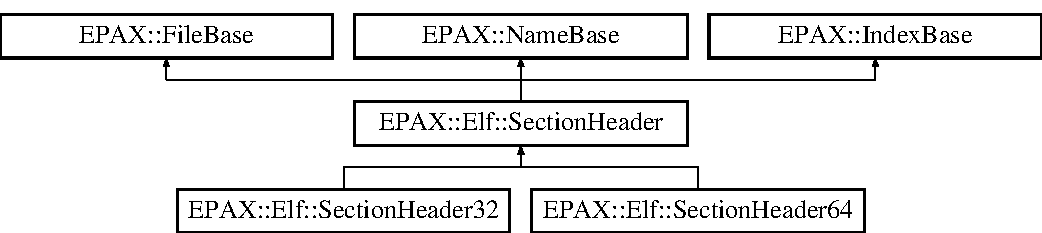
\includegraphics[height=3.000000cm]{class_e_p_a_x_1_1_elf_1_1_section_header}
\end{center}
\end{figure}
\subsection*{\-Public \-Member \-Functions}
\begin{DoxyCompactItemize}
\item 
\hyperlink{class_e_p_a_x_1_1_elf_1_1_section_header_a54cc02de71e0399deb189afa5261f69a}{\-Section\-Header} (\hyperlink{class_e_p_a_x_1_1_base_binary}{\-Base\-Binary} $\ast$b, uint64\-\_\-t o, uint64\-\_\-t s, uint32\-\_\-t i)
\item 
virtual \hyperlink{class_e_p_a_x_1_1_elf_1_1_section_header_a6e422772b689a748bd07d9e432419b72}{$\sim$\-Section\-Header} ()
\item 
void \hyperlink{class_e_p_a_x_1_1_elf_1_1_section_header_a52fc6666a33be6852fbcc6894cc3d655}{print} (std\-::ostream \&stream=std\-::cout)
\item 
bool \hyperlink{class_e_p_a_x_1_1_elf_1_1_section_header_adf62f9619c5cdbe66524f864db451e26}{is\-Text} ()
\item 
bool \hyperlink{class_e_p_a_x_1_1_elf_1_1_section_header_ad554ff1dd465817c89bc817ac4e5d307}{is\-Data} ()
\item 
bool \hyperlink{class_e_p_a_x_1_1_elf_1_1_section_header_aeb485b30076f37e8ebc7c46e14c239f9}{is\-B\-S\-S} ()
\item 
bool \hyperlink{class_e_p_a_x_1_1_elf_1_1_section_header_ab1e8c09b12f6e5caef352d2eb32b7b7d}{is\-Debug} ()
\item 
bool \hyperlink{class_e_p_a_x_1_1_elf_1_1_section_header_a6d66cd345b7cb520d758ae04c50164e1}{is\-String} ()
\item 
bool \hyperlink{class_e_p_a_x_1_1_elf_1_1_section_header_a9320f92c5158659c148ee6f197b0cd70}{is\-Symbol} ()
\item 
bool \hyperlink{class_e_p_a_x_1_1_elf_1_1_section_header_ae6a3998c6af4e70913fa7bb1dd17642d}{is\-Read} ()
\item 
bool \hyperlink{class_e_p_a_x_1_1_elf_1_1_section_header_a5e33ad1689cd25b074f81397148bfd96}{is\-Write} ()
\item 
bool \hyperlink{class_e_p_a_x_1_1_elf_1_1_section_header_af6c441b3851a2311ad73a4ca3a550f33}{is\-Exec} ()
\item 
bool \hyperlink{class_e_p_a_x_1_1_elf_1_1_section_header_a31d2e329b17565b128798f80ed0779e1}{is\-Alloc} ()
\item 
bool \hyperlink{class_e_p_a_x_1_1_elf_1_1_section_header_aac6b62764b01dceae67f5fff1c966a70}{is\-Merge} ()
\item 
bool \hyperlink{class_e_p_a_x_1_1_elf_1_1_section_header_aaeba234d199df23d8be4ab874e6a8bac}{in\-Range} (uint64\-\_\-t a)
\item 
virtual uint64\-\_\-t \hyperlink{class_e_p_a_x_1_1_elf_1_1_section_header_aac92cdabd70a208e45ff0b6920bee3e6}{get\-Name\-Index} ()=0
\item 
virtual uint64\-\_\-t \hyperlink{class_e_p_a_x_1_1_elf_1_1_section_header_af7e6230e8d4b68886ef8dcda238f1072}{get\-Type} ()=0
\item 
virtual uint64\-\_\-t \hyperlink{class_e_p_a_x_1_1_elf_1_1_section_header_a34bc5ee9fc05b1780e8cca68828bfc23}{get\-Virt\-Addr} ()=0
\item 
virtual uint64\-\_\-t \hyperlink{class_e_p_a_x_1_1_elf_1_1_section_header_a1beecb645d931ff31696e9994f1f0e06}{get\-File\-Offset} ()=0
\item 
virtual uint64\-\_\-t \hyperlink{class_e_p_a_x_1_1_elf_1_1_section_header_a035451e10f87faae8d772f8fda9e42d0}{get\-Section\-Link} ()=0
\item 
virtual uint64\-\_\-t \hyperlink{class_e_p_a_x_1_1_elf_1_1_section_header_a65a863f2eb15aa211d772fc1b3013d64}{get\-Alignment} ()=0
\item 
virtual uint64\-\_\-t \hyperlink{class_e_p_a_x_1_1_elf_1_1_section_header_a97327fc2deb88d4873bfa36b25864567}{get\-Entry\-Size} ()=0
\item 
virtual uint64\-\_\-t \hyperlink{class_e_p_a_x_1_1_elf_1_1_section_header_ab573a5f4b64afd5dc7f5b835c5b1becf}{get\-Flags} ()=0
\item 
virtual uint64\-\_\-t \hyperlink{class_e_p_a_x_1_1_elf_1_1_section_header_a2d9cd842c34c4075260116f0ab373fa2}{get\-Size} ()=0
\end{DoxyCompactItemize}
\subsection*{\-Protected \-Attributes}
\begin{DoxyCompactItemize}
\item 
\hyperlink{_e_p_a_x_common_internal_8hpp_a17755bdd71c02e656c667b16de61dd7b}{rawbyte\-\_\-t} $\ast$ \hyperlink{class_e_p_a_x_1_1_elf_1_1_section_header_a84d8a573ab3f70298e15d46e83197260}{entry}
\end{DoxyCompactItemize}


\subsection{\-Detailed \-Description}


\-Definition at line 248 of file \-Elf\-Binary.\-hpp.



\subsection{\-Constructor \& \-Destructor \-Documentation}
\hypertarget{class_e_p_a_x_1_1_elf_1_1_section_header_a54cc02de71e0399deb189afa5261f69a}{\index{\-E\-P\-A\-X\-::\-Elf\-::\-Section\-Header@{\-E\-P\-A\-X\-::\-Elf\-::\-Section\-Header}!\-Section\-Header@{\-Section\-Header}}
\index{\-Section\-Header@{\-Section\-Header}!EPAX::Elf::SectionHeader@{\-E\-P\-A\-X\-::\-Elf\-::\-Section\-Header}}
\subsubsection[{\-Section\-Header}]{\setlength{\rightskip}{0pt plus 5cm}{\bf \-E\-P\-A\-X\-::\-Elf\-::\-Section\-Header\-::\-Section\-Header} (
\begin{DoxyParamCaption}
\item[{{\bf \-Base\-Binary} $\ast$}]{b, }
\item[{uint64\-\_\-t}]{o, }
\item[{uint64\-\_\-t}]{s, }
\item[{uint32\-\_\-t}]{i}
\end{DoxyParamCaption}
)}}\label{class_e_p_a_x_1_1_elf_1_1_section_header_a54cc02de71e0399deb189afa5261f69a}


\-Definition at line 677 of file \-Elf\-Binary.\-cpp.

\hypertarget{class_e_p_a_x_1_1_elf_1_1_section_header_a6e422772b689a748bd07d9e432419b72}{\index{\-E\-P\-A\-X\-::\-Elf\-::\-Section\-Header@{\-E\-P\-A\-X\-::\-Elf\-::\-Section\-Header}!$\sim$\-Section\-Header@{$\sim$\-Section\-Header}}
\index{$\sim$\-Section\-Header@{$\sim$\-Section\-Header}!EPAX::Elf::SectionHeader@{\-E\-P\-A\-X\-::\-Elf\-::\-Section\-Header}}
\subsubsection[{$\sim$\-Section\-Header}]{\setlength{\rightskip}{0pt plus 5cm}{\bf \-E\-P\-A\-X\-::\-Elf\-::\-Section\-Header\-::$\sim$\-Section\-Header} (
\begin{DoxyParamCaption}
{}
\end{DoxyParamCaption}
)\hspace{0.3cm}{\ttfamily  \mbox{[}virtual\mbox{]}}}}\label{class_e_p_a_x_1_1_elf_1_1_section_header_a6e422772b689a748bd07d9e432419b72}


\-Definition at line 685 of file \-Elf\-Binary.\-cpp.



\subsection{\-Member \-Function \-Documentation}
\hypertarget{class_e_p_a_x_1_1_elf_1_1_section_header_a65a863f2eb15aa211d772fc1b3013d64}{\index{\-E\-P\-A\-X\-::\-Elf\-::\-Section\-Header@{\-E\-P\-A\-X\-::\-Elf\-::\-Section\-Header}!get\-Alignment@{get\-Alignment}}
\index{get\-Alignment@{get\-Alignment}!EPAX::Elf::SectionHeader@{\-E\-P\-A\-X\-::\-Elf\-::\-Section\-Header}}
\subsubsection[{get\-Alignment}]{\setlength{\rightskip}{0pt plus 5cm}virtual uint64\-\_\-t {\bf \-E\-P\-A\-X\-::\-Elf\-::\-Section\-Header\-::get\-Alignment} (
\begin{DoxyParamCaption}
{}
\end{DoxyParamCaption}
)\hspace{0.3cm}{\ttfamily  \mbox{[}pure virtual\mbox{]}}}}\label{class_e_p_a_x_1_1_elf_1_1_section_header_a65a863f2eb15aa211d772fc1b3013d64}


\-Implemented in \hyperlink{class_e_p_a_x_1_1_elf_1_1_section_header64_a8efa6c61a662689bd23732884b4a9aa5}{\-E\-P\-A\-X\-::\-Elf\-::\-Section\-Header64}, and \hyperlink{class_e_p_a_x_1_1_elf_1_1_section_header32_a36d45234fbdfd27ac89e449f0084e985}{\-E\-P\-A\-X\-::\-Elf\-::\-Section\-Header32}.

\hypertarget{class_e_p_a_x_1_1_elf_1_1_section_header_a97327fc2deb88d4873bfa36b25864567}{\index{\-E\-P\-A\-X\-::\-Elf\-::\-Section\-Header@{\-E\-P\-A\-X\-::\-Elf\-::\-Section\-Header}!get\-Entry\-Size@{get\-Entry\-Size}}
\index{get\-Entry\-Size@{get\-Entry\-Size}!EPAX::Elf::SectionHeader@{\-E\-P\-A\-X\-::\-Elf\-::\-Section\-Header}}
\subsubsection[{get\-Entry\-Size}]{\setlength{\rightskip}{0pt plus 5cm}virtual uint64\-\_\-t {\bf \-E\-P\-A\-X\-::\-Elf\-::\-Section\-Header\-::get\-Entry\-Size} (
\begin{DoxyParamCaption}
{}
\end{DoxyParamCaption}
)\hspace{0.3cm}{\ttfamily  \mbox{[}pure virtual\mbox{]}}}}\label{class_e_p_a_x_1_1_elf_1_1_section_header_a97327fc2deb88d4873bfa36b25864567}


\-Implemented in \hyperlink{class_e_p_a_x_1_1_elf_1_1_section_header64_a3b16015c2864179254466fa389a5b90e}{\-E\-P\-A\-X\-::\-Elf\-::\-Section\-Header64}, and \hyperlink{class_e_p_a_x_1_1_elf_1_1_section_header32_adbddf01ab8a4115d7c07dfe92e2160c6}{\-E\-P\-A\-X\-::\-Elf\-::\-Section\-Header32}.

\hypertarget{class_e_p_a_x_1_1_elf_1_1_section_header_a1beecb645d931ff31696e9994f1f0e06}{\index{\-E\-P\-A\-X\-::\-Elf\-::\-Section\-Header@{\-E\-P\-A\-X\-::\-Elf\-::\-Section\-Header}!get\-File\-Offset@{get\-File\-Offset}}
\index{get\-File\-Offset@{get\-File\-Offset}!EPAX::Elf::SectionHeader@{\-E\-P\-A\-X\-::\-Elf\-::\-Section\-Header}}
\subsubsection[{get\-File\-Offset}]{\setlength{\rightskip}{0pt plus 5cm}virtual uint64\-\_\-t {\bf \-E\-P\-A\-X\-::\-Elf\-::\-Section\-Header\-::get\-File\-Offset} (
\begin{DoxyParamCaption}
{}
\end{DoxyParamCaption}
)\hspace{0.3cm}{\ttfamily  \mbox{[}pure virtual\mbox{]}}}}\label{class_e_p_a_x_1_1_elf_1_1_section_header_a1beecb645d931ff31696e9994f1f0e06}


\-Reimplemented from \hyperlink{class_e_p_a_x_1_1_file_base_a779f2254eef1279f52f372e18bfb75f7}{\-E\-P\-A\-X\-::\-File\-Base}.



\-Implemented in \hyperlink{class_e_p_a_x_1_1_elf_1_1_section_header64_acd9363817d1fbab5194a3da55e8a7240}{\-E\-P\-A\-X\-::\-Elf\-::\-Section\-Header64}, and \hyperlink{class_e_p_a_x_1_1_elf_1_1_section_header32_a10cf04485e82a2f38b852732345dcd29}{\-E\-P\-A\-X\-::\-Elf\-::\-Section\-Header32}.

\hypertarget{class_e_p_a_x_1_1_elf_1_1_section_header_ab573a5f4b64afd5dc7f5b835c5b1becf}{\index{\-E\-P\-A\-X\-::\-Elf\-::\-Section\-Header@{\-E\-P\-A\-X\-::\-Elf\-::\-Section\-Header}!get\-Flags@{get\-Flags}}
\index{get\-Flags@{get\-Flags}!EPAX::Elf::SectionHeader@{\-E\-P\-A\-X\-::\-Elf\-::\-Section\-Header}}
\subsubsection[{get\-Flags}]{\setlength{\rightskip}{0pt plus 5cm}virtual uint64\-\_\-t {\bf \-E\-P\-A\-X\-::\-Elf\-::\-Section\-Header\-::get\-Flags} (
\begin{DoxyParamCaption}
{}
\end{DoxyParamCaption}
)\hspace{0.3cm}{\ttfamily  \mbox{[}pure virtual\mbox{]}}}}\label{class_e_p_a_x_1_1_elf_1_1_section_header_ab573a5f4b64afd5dc7f5b835c5b1becf}


\-Implemented in \hyperlink{class_e_p_a_x_1_1_elf_1_1_section_header64_a4ca003bc2633ba8e16824a0d6f9f5dd1}{\-E\-P\-A\-X\-::\-Elf\-::\-Section\-Header64}, and \hyperlink{class_e_p_a_x_1_1_elf_1_1_section_header32_a6235f57290293d0836cee2adadf7c924}{\-E\-P\-A\-X\-::\-Elf\-::\-Section\-Header32}.

\hypertarget{class_e_p_a_x_1_1_elf_1_1_section_header_aac92cdabd70a208e45ff0b6920bee3e6}{\index{\-E\-P\-A\-X\-::\-Elf\-::\-Section\-Header@{\-E\-P\-A\-X\-::\-Elf\-::\-Section\-Header}!get\-Name\-Index@{get\-Name\-Index}}
\index{get\-Name\-Index@{get\-Name\-Index}!EPAX::Elf::SectionHeader@{\-E\-P\-A\-X\-::\-Elf\-::\-Section\-Header}}
\subsubsection[{get\-Name\-Index}]{\setlength{\rightskip}{0pt plus 5cm}virtual uint64\-\_\-t {\bf \-E\-P\-A\-X\-::\-Elf\-::\-Section\-Header\-::get\-Name\-Index} (
\begin{DoxyParamCaption}
{}
\end{DoxyParamCaption}
)\hspace{0.3cm}{\ttfamily  \mbox{[}pure virtual\mbox{]}}}}\label{class_e_p_a_x_1_1_elf_1_1_section_header_aac92cdabd70a208e45ff0b6920bee3e6}


\-Implemented in \hyperlink{class_e_p_a_x_1_1_elf_1_1_section_header64_a4c83a831f07f96738a32fefd2f55b669}{\-E\-P\-A\-X\-::\-Elf\-::\-Section\-Header64}, and \hyperlink{class_e_p_a_x_1_1_elf_1_1_section_header32_a03ea8c9bb8bb24b88f75158085ef557e}{\-E\-P\-A\-X\-::\-Elf\-::\-Section\-Header32}.

\hypertarget{class_e_p_a_x_1_1_elf_1_1_section_header_a035451e10f87faae8d772f8fda9e42d0}{\index{\-E\-P\-A\-X\-::\-Elf\-::\-Section\-Header@{\-E\-P\-A\-X\-::\-Elf\-::\-Section\-Header}!get\-Section\-Link@{get\-Section\-Link}}
\index{get\-Section\-Link@{get\-Section\-Link}!EPAX::Elf::SectionHeader@{\-E\-P\-A\-X\-::\-Elf\-::\-Section\-Header}}
\subsubsection[{get\-Section\-Link}]{\setlength{\rightskip}{0pt plus 5cm}virtual uint64\-\_\-t {\bf \-E\-P\-A\-X\-::\-Elf\-::\-Section\-Header\-::get\-Section\-Link} (
\begin{DoxyParamCaption}
{}
\end{DoxyParamCaption}
)\hspace{0.3cm}{\ttfamily  \mbox{[}pure virtual\mbox{]}}}}\label{class_e_p_a_x_1_1_elf_1_1_section_header_a035451e10f87faae8d772f8fda9e42d0}


\-Implemented in \hyperlink{class_e_p_a_x_1_1_elf_1_1_section_header64_aed1f49f68dc2b948fb8c5fe7d6df6ec5}{\-E\-P\-A\-X\-::\-Elf\-::\-Section\-Header64}, and \hyperlink{class_e_p_a_x_1_1_elf_1_1_section_header32_ad60ce4da7aa979dcf82115920f3b3664}{\-E\-P\-A\-X\-::\-Elf\-::\-Section\-Header32}.

\hypertarget{class_e_p_a_x_1_1_elf_1_1_section_header_a2d9cd842c34c4075260116f0ab373fa2}{\index{\-E\-P\-A\-X\-::\-Elf\-::\-Section\-Header@{\-E\-P\-A\-X\-::\-Elf\-::\-Section\-Header}!get\-Size@{get\-Size}}
\index{get\-Size@{get\-Size}!EPAX::Elf::SectionHeader@{\-E\-P\-A\-X\-::\-Elf\-::\-Section\-Header}}
\subsubsection[{get\-Size}]{\setlength{\rightskip}{0pt plus 5cm}virtual uint64\-\_\-t {\bf \-E\-P\-A\-X\-::\-Elf\-::\-Section\-Header\-::get\-Size} (
\begin{DoxyParamCaption}
{}
\end{DoxyParamCaption}
)\hspace{0.3cm}{\ttfamily  \mbox{[}pure virtual\mbox{]}}}}\label{class_e_p_a_x_1_1_elf_1_1_section_header_a2d9cd842c34c4075260116f0ab373fa2}


\-Implemented in \hyperlink{class_e_p_a_x_1_1_elf_1_1_section_header64_a0b4f7cd68d065481a6953240f55f8073}{\-E\-P\-A\-X\-::\-Elf\-::\-Section\-Header64}, and \hyperlink{class_e_p_a_x_1_1_elf_1_1_section_header32_a04f7dbe427fb6c19261b5de7cbacfd05}{\-E\-P\-A\-X\-::\-Elf\-::\-Section\-Header32}.

\hypertarget{class_e_p_a_x_1_1_elf_1_1_section_header_af7e6230e8d4b68886ef8dcda238f1072}{\index{\-E\-P\-A\-X\-::\-Elf\-::\-Section\-Header@{\-E\-P\-A\-X\-::\-Elf\-::\-Section\-Header}!get\-Type@{get\-Type}}
\index{get\-Type@{get\-Type}!EPAX::Elf::SectionHeader@{\-E\-P\-A\-X\-::\-Elf\-::\-Section\-Header}}
\subsubsection[{get\-Type}]{\setlength{\rightskip}{0pt plus 5cm}virtual uint64\-\_\-t {\bf \-E\-P\-A\-X\-::\-Elf\-::\-Section\-Header\-::get\-Type} (
\begin{DoxyParamCaption}
{}
\end{DoxyParamCaption}
)\hspace{0.3cm}{\ttfamily  \mbox{[}pure virtual\mbox{]}}}}\label{class_e_p_a_x_1_1_elf_1_1_section_header_af7e6230e8d4b68886ef8dcda238f1072}


\-Implemented in \hyperlink{class_e_p_a_x_1_1_elf_1_1_section_header64_a8556b692a71aba5e1048a7152cb1d837}{\-E\-P\-A\-X\-::\-Elf\-::\-Section\-Header64}, and \hyperlink{class_e_p_a_x_1_1_elf_1_1_section_header32_a84ed73ec4cb58e9919222a884dbe0cd3}{\-E\-P\-A\-X\-::\-Elf\-::\-Section\-Header32}.

\hypertarget{class_e_p_a_x_1_1_elf_1_1_section_header_a34bc5ee9fc05b1780e8cca68828bfc23}{\index{\-E\-P\-A\-X\-::\-Elf\-::\-Section\-Header@{\-E\-P\-A\-X\-::\-Elf\-::\-Section\-Header}!get\-Virt\-Addr@{get\-Virt\-Addr}}
\index{get\-Virt\-Addr@{get\-Virt\-Addr}!EPAX::Elf::SectionHeader@{\-E\-P\-A\-X\-::\-Elf\-::\-Section\-Header}}
\subsubsection[{get\-Virt\-Addr}]{\setlength{\rightskip}{0pt plus 5cm}virtual uint64\-\_\-t {\bf \-E\-P\-A\-X\-::\-Elf\-::\-Section\-Header\-::get\-Virt\-Addr} (
\begin{DoxyParamCaption}
{}
\end{DoxyParamCaption}
)\hspace{0.3cm}{\ttfamily  \mbox{[}pure virtual\mbox{]}}}}\label{class_e_p_a_x_1_1_elf_1_1_section_header_a34bc5ee9fc05b1780e8cca68828bfc23}


\-Implemented in \hyperlink{class_e_p_a_x_1_1_elf_1_1_section_header64_a5d82c8c6748a80bb0d53b8d6a6a9c3fb}{\-E\-P\-A\-X\-::\-Elf\-::\-Section\-Header64}, and \hyperlink{class_e_p_a_x_1_1_elf_1_1_section_header32_a0d804e41f351baa2a0165e705e84ce86}{\-E\-P\-A\-X\-::\-Elf\-::\-Section\-Header32}.

\hypertarget{class_e_p_a_x_1_1_elf_1_1_section_header_aaeba234d199df23d8be4ab874e6a8bac}{\index{\-E\-P\-A\-X\-::\-Elf\-::\-Section\-Header@{\-E\-P\-A\-X\-::\-Elf\-::\-Section\-Header}!in\-Range@{in\-Range}}
\index{in\-Range@{in\-Range}!EPAX::Elf::SectionHeader@{\-E\-P\-A\-X\-::\-Elf\-::\-Section\-Header}}
\subsubsection[{in\-Range}]{\setlength{\rightskip}{0pt plus 5cm}bool {\bf \-E\-P\-A\-X\-::\-Elf\-::\-Section\-Header\-::in\-Range} (
\begin{DoxyParamCaption}
\item[{uint64\-\_\-t}]{a}
\end{DoxyParamCaption}
)}}\label{class_e_p_a_x_1_1_elf_1_1_section_header_aaeba234d199df23d8be4ab874e6a8bac}


\-Definition at line 736 of file \-Elf\-Binary.\-cpp.

\hypertarget{class_e_p_a_x_1_1_elf_1_1_section_header_a31d2e329b17565b128798f80ed0779e1}{\index{\-E\-P\-A\-X\-::\-Elf\-::\-Section\-Header@{\-E\-P\-A\-X\-::\-Elf\-::\-Section\-Header}!is\-Alloc@{is\-Alloc}}
\index{is\-Alloc@{is\-Alloc}!EPAX::Elf::SectionHeader@{\-E\-P\-A\-X\-::\-Elf\-::\-Section\-Header}}
\subsubsection[{is\-Alloc}]{\setlength{\rightskip}{0pt plus 5cm}bool {\bf \-E\-P\-A\-X\-::\-Elf\-::\-Section\-Header\-::is\-Alloc} (
\begin{DoxyParamCaption}
{}
\end{DoxyParamCaption}
)}}\label{class_e_p_a_x_1_1_elf_1_1_section_header_a31d2e329b17565b128798f80ed0779e1}


\-Definition at line 779 of file \-Elf\-Binary.\-cpp.

\hypertarget{class_e_p_a_x_1_1_elf_1_1_section_header_aeb485b30076f37e8ebc7c46e14c239f9}{\index{\-E\-P\-A\-X\-::\-Elf\-::\-Section\-Header@{\-E\-P\-A\-X\-::\-Elf\-::\-Section\-Header}!is\-B\-S\-S@{is\-B\-S\-S}}
\index{is\-B\-S\-S@{is\-B\-S\-S}!EPAX::Elf::SectionHeader@{\-E\-P\-A\-X\-::\-Elf\-::\-Section\-Header}}
\subsubsection[{is\-B\-S\-S}]{\setlength{\rightskip}{0pt plus 5cm}bool {\bf \-E\-P\-A\-X\-::\-Elf\-::\-Section\-Header\-::is\-B\-S\-S} (
\begin{DoxyParamCaption}
{}
\end{DoxyParamCaption}
)}}\label{class_e_p_a_x_1_1_elf_1_1_section_header_aeb485b30076f37e8ebc7c46e14c239f9}


\-Definition at line 751 of file \-Elf\-Binary.\-cpp.

\hypertarget{class_e_p_a_x_1_1_elf_1_1_section_header_ad554ff1dd465817c89bc817ac4e5d307}{\index{\-E\-P\-A\-X\-::\-Elf\-::\-Section\-Header@{\-E\-P\-A\-X\-::\-Elf\-::\-Section\-Header}!is\-Data@{is\-Data}}
\index{is\-Data@{is\-Data}!EPAX::Elf::SectionHeader@{\-E\-P\-A\-X\-::\-Elf\-::\-Section\-Header}}
\subsubsection[{is\-Data}]{\setlength{\rightskip}{0pt plus 5cm}bool {\bf \-E\-P\-A\-X\-::\-Elf\-::\-Section\-Header\-::is\-Data} (
\begin{DoxyParamCaption}
{}
\end{DoxyParamCaption}
)}}\label{class_e_p_a_x_1_1_elf_1_1_section_header_ad554ff1dd465817c89bc817ac4e5d307}


\-Definition at line 747 of file \-Elf\-Binary.\-cpp.

\hypertarget{class_e_p_a_x_1_1_elf_1_1_section_header_ab1e8c09b12f6e5caef352d2eb32b7b7d}{\index{\-E\-P\-A\-X\-::\-Elf\-::\-Section\-Header@{\-E\-P\-A\-X\-::\-Elf\-::\-Section\-Header}!is\-Debug@{is\-Debug}}
\index{is\-Debug@{is\-Debug}!EPAX::Elf::SectionHeader@{\-E\-P\-A\-X\-::\-Elf\-::\-Section\-Header}}
\subsubsection[{is\-Debug}]{\setlength{\rightskip}{0pt plus 5cm}bool {\bf \-E\-P\-A\-X\-::\-Elf\-::\-Section\-Header\-::is\-Debug} (
\begin{DoxyParamCaption}
{}
\end{DoxyParamCaption}
)}}\label{class_e_p_a_x_1_1_elf_1_1_section_header_ab1e8c09b12f6e5caef352d2eb32b7b7d}


\-Definition at line 755 of file \-Elf\-Binary.\-cpp.

\hypertarget{class_e_p_a_x_1_1_elf_1_1_section_header_af6c441b3851a2311ad73a4ca3a550f33}{\index{\-E\-P\-A\-X\-::\-Elf\-::\-Section\-Header@{\-E\-P\-A\-X\-::\-Elf\-::\-Section\-Header}!is\-Exec@{is\-Exec}}
\index{is\-Exec@{is\-Exec}!EPAX::Elf::SectionHeader@{\-E\-P\-A\-X\-::\-Elf\-::\-Section\-Header}}
\subsubsection[{is\-Exec}]{\setlength{\rightskip}{0pt plus 5cm}bool {\bf \-E\-P\-A\-X\-::\-Elf\-::\-Section\-Header\-::is\-Exec} (
\begin{DoxyParamCaption}
{}
\end{DoxyParamCaption}
)}}\label{class_e_p_a_x_1_1_elf_1_1_section_header_af6c441b3851a2311ad73a4ca3a550f33}


\-Definition at line 775 of file \-Elf\-Binary.\-cpp.

\hypertarget{class_e_p_a_x_1_1_elf_1_1_section_header_aac6b62764b01dceae67f5fff1c966a70}{\index{\-E\-P\-A\-X\-::\-Elf\-::\-Section\-Header@{\-E\-P\-A\-X\-::\-Elf\-::\-Section\-Header}!is\-Merge@{is\-Merge}}
\index{is\-Merge@{is\-Merge}!EPAX::Elf::SectionHeader@{\-E\-P\-A\-X\-::\-Elf\-::\-Section\-Header}}
\subsubsection[{is\-Merge}]{\setlength{\rightskip}{0pt plus 5cm}bool {\bf \-E\-P\-A\-X\-::\-Elf\-::\-Section\-Header\-::is\-Merge} (
\begin{DoxyParamCaption}
{}
\end{DoxyParamCaption}
)}}\label{class_e_p_a_x_1_1_elf_1_1_section_header_aac6b62764b01dceae67f5fff1c966a70}


\-Definition at line 783 of file \-Elf\-Binary.\-cpp.

\hypertarget{class_e_p_a_x_1_1_elf_1_1_section_header_ae6a3998c6af4e70913fa7bb1dd17642d}{\index{\-E\-P\-A\-X\-::\-Elf\-::\-Section\-Header@{\-E\-P\-A\-X\-::\-Elf\-::\-Section\-Header}!is\-Read@{is\-Read}}
\index{is\-Read@{is\-Read}!EPAX::Elf::SectionHeader@{\-E\-P\-A\-X\-::\-Elf\-::\-Section\-Header}}
\subsubsection[{is\-Read}]{\setlength{\rightskip}{0pt plus 5cm}bool {\bf \-E\-P\-A\-X\-::\-Elf\-::\-Section\-Header\-::is\-Read} (
\begin{DoxyParamCaption}
{}
\end{DoxyParamCaption}
)}}\label{class_e_p_a_x_1_1_elf_1_1_section_header_ae6a3998c6af4e70913fa7bb1dd17642d}


\-Definition at line 767 of file \-Elf\-Binary.\-cpp.

\hypertarget{class_e_p_a_x_1_1_elf_1_1_section_header_a6d66cd345b7cb520d758ae04c50164e1}{\index{\-E\-P\-A\-X\-::\-Elf\-::\-Section\-Header@{\-E\-P\-A\-X\-::\-Elf\-::\-Section\-Header}!is\-String@{is\-String}}
\index{is\-String@{is\-String}!EPAX::Elf::SectionHeader@{\-E\-P\-A\-X\-::\-Elf\-::\-Section\-Header}}
\subsubsection[{is\-String}]{\setlength{\rightskip}{0pt plus 5cm}bool {\bf \-E\-P\-A\-X\-::\-Elf\-::\-Section\-Header\-::is\-String} (
\begin{DoxyParamCaption}
{}
\end{DoxyParamCaption}
)}}\label{class_e_p_a_x_1_1_elf_1_1_section_header_a6d66cd345b7cb520d758ae04c50164e1}


\-Definition at line 759 of file \-Elf\-Binary.\-cpp.

\hypertarget{class_e_p_a_x_1_1_elf_1_1_section_header_a9320f92c5158659c148ee6f197b0cd70}{\index{\-E\-P\-A\-X\-::\-Elf\-::\-Section\-Header@{\-E\-P\-A\-X\-::\-Elf\-::\-Section\-Header}!is\-Symbol@{is\-Symbol}}
\index{is\-Symbol@{is\-Symbol}!EPAX::Elf::SectionHeader@{\-E\-P\-A\-X\-::\-Elf\-::\-Section\-Header}}
\subsubsection[{is\-Symbol}]{\setlength{\rightskip}{0pt plus 5cm}bool {\bf \-E\-P\-A\-X\-::\-Elf\-::\-Section\-Header\-::is\-Symbol} (
\begin{DoxyParamCaption}
{}
\end{DoxyParamCaption}
)}}\label{class_e_p_a_x_1_1_elf_1_1_section_header_a9320f92c5158659c148ee6f197b0cd70}


\-Definition at line 763 of file \-Elf\-Binary.\-cpp.

\hypertarget{class_e_p_a_x_1_1_elf_1_1_section_header_adf62f9619c5cdbe66524f864db451e26}{\index{\-E\-P\-A\-X\-::\-Elf\-::\-Section\-Header@{\-E\-P\-A\-X\-::\-Elf\-::\-Section\-Header}!is\-Text@{is\-Text}}
\index{is\-Text@{is\-Text}!EPAX::Elf::SectionHeader@{\-E\-P\-A\-X\-::\-Elf\-::\-Section\-Header}}
\subsubsection[{is\-Text}]{\setlength{\rightskip}{0pt plus 5cm}bool {\bf \-E\-P\-A\-X\-::\-Elf\-::\-Section\-Header\-::is\-Text} (
\begin{DoxyParamCaption}
{}
\end{DoxyParamCaption}
)}}\label{class_e_p_a_x_1_1_elf_1_1_section_header_adf62f9619c5cdbe66524f864db451e26}


\-Definition at line 743 of file \-Elf\-Binary.\-cpp.

\hypertarget{class_e_p_a_x_1_1_elf_1_1_section_header_a5e33ad1689cd25b074f81397148bfd96}{\index{\-E\-P\-A\-X\-::\-Elf\-::\-Section\-Header@{\-E\-P\-A\-X\-::\-Elf\-::\-Section\-Header}!is\-Write@{is\-Write}}
\index{is\-Write@{is\-Write}!EPAX::Elf::SectionHeader@{\-E\-P\-A\-X\-::\-Elf\-::\-Section\-Header}}
\subsubsection[{is\-Write}]{\setlength{\rightskip}{0pt plus 5cm}bool {\bf \-E\-P\-A\-X\-::\-Elf\-::\-Section\-Header\-::is\-Write} (
\begin{DoxyParamCaption}
{}
\end{DoxyParamCaption}
)}}\label{class_e_p_a_x_1_1_elf_1_1_section_header_a5e33ad1689cd25b074f81397148bfd96}


\-Definition at line 771 of file \-Elf\-Binary.\-cpp.

\hypertarget{class_e_p_a_x_1_1_elf_1_1_section_header_a52fc6666a33be6852fbcc6894cc3d655}{\index{\-E\-P\-A\-X\-::\-Elf\-::\-Section\-Header@{\-E\-P\-A\-X\-::\-Elf\-::\-Section\-Header}!print@{print}}
\index{print@{print}!EPAX::Elf::SectionHeader@{\-E\-P\-A\-X\-::\-Elf\-::\-Section\-Header}}
\subsubsection[{print}]{\setlength{\rightskip}{0pt plus 5cm}void {\bf \-E\-P\-A\-X\-::\-Elf\-::\-Section\-Header\-::print} (
\begin{DoxyParamCaption}
\item[{std\-::ostream \&}]{stream = {\ttfamily std\-:\-:cout}}
\end{DoxyParamCaption}
)}}\label{class_e_p_a_x_1_1_elf_1_1_section_header_a52fc6666a33be6852fbcc6894cc3d655}


\-Definition at line 724 of file \-Elf\-Binary.\-cpp.



\subsection{\-Member \-Data \-Documentation}
\hypertarget{class_e_p_a_x_1_1_elf_1_1_section_header_a84d8a573ab3f70298e15d46e83197260}{\index{\-E\-P\-A\-X\-::\-Elf\-::\-Section\-Header@{\-E\-P\-A\-X\-::\-Elf\-::\-Section\-Header}!entry@{entry}}
\index{entry@{entry}!EPAX::Elf::SectionHeader@{\-E\-P\-A\-X\-::\-Elf\-::\-Section\-Header}}
\subsubsection[{entry}]{\setlength{\rightskip}{0pt plus 5cm}{\bf rawbyte\-\_\-t}$\ast$ {\bf \-E\-P\-A\-X\-::\-Elf\-::\-Section\-Header\-::entry}\hspace{0.3cm}{\ttfamily  \mbox{[}protected\mbox{]}}}}\label{class_e_p_a_x_1_1_elf_1_1_section_header_a84d8a573ab3f70298e15d46e83197260}


\-Definition at line 250 of file \-Elf\-Binary.\-hpp.



\-The documentation for this class was generated from the following files\-:\begin{DoxyCompactItemize}
\item 
\hyperlink{_elf_binary_8hpp}{\-Elf\-Binary.\-hpp}\item 
\hyperlink{_elf_binary_8cpp}{\-Elf\-Binary.\-cpp}\end{DoxyCompactItemize}

\hypertarget{class_e_p_a_x_1_1_elf_1_1_section_header32}{\section{\-E\-P\-A\-X\-:\-:\-Elf\-:\-:\-Section\-Header32 \-Class \-Reference}
\label{class_e_p_a_x_1_1_elf_1_1_section_header32}\index{\-E\-P\-A\-X\-::\-Elf\-::\-Section\-Header32@{\-E\-P\-A\-X\-::\-Elf\-::\-Section\-Header32}}
}


{\ttfamily \#include $<$\-Elf\-Binary.\-hpp$>$}

\-Inheritance diagram for \-E\-P\-A\-X\-:\-:\-Elf\-:\-:\-Section\-Header32\-:\begin{figure}[H]
\begin{center}
\leavevmode
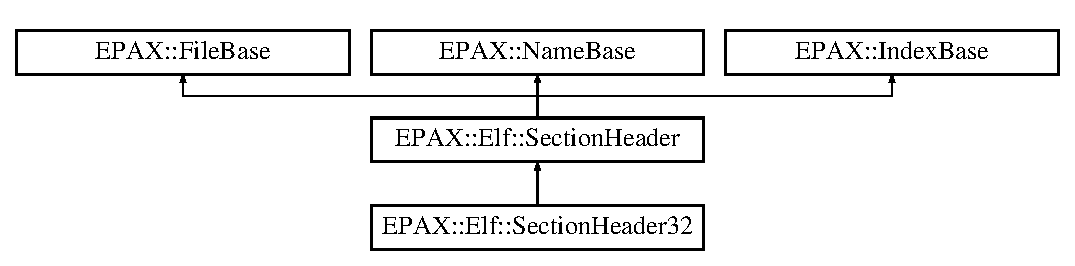
\includegraphics[height=3.000000cm]{class_e_p_a_x_1_1_elf_1_1_section_header32}
\end{center}
\end{figure}
\subsection*{\-Public \-Member \-Functions}
\begin{DoxyCompactItemize}
\item 
\hyperlink{class_e_p_a_x_1_1_elf_1_1_section_header32_a03a69e255bde29bc1c035fd8a3800e0d}{\-Section\-Header32} (\hyperlink{class_e_p_a_x_1_1_base_binary}{\-Base\-Binary} $\ast$b, uint64\-\_\-t o, uint64\-\_\-t s, uint32\-\_\-t i)
\item 
virtual \hyperlink{class_e_p_a_x_1_1_elf_1_1_section_header32_ad40d1aaf6684064eb553cf6eea466773}{$\sim$\-Section\-Header32} ()
\item 
uint64\-\_\-t \hyperlink{class_e_p_a_x_1_1_elf_1_1_section_header32_a03ea8c9bb8bb24b88f75158085ef557e}{get\-Name\-Index} ()
\item 
uint64\-\_\-t \hyperlink{class_e_p_a_x_1_1_elf_1_1_section_header32_a84ed73ec4cb58e9919222a884dbe0cd3}{get\-Type} ()
\item 
uint64\-\_\-t \hyperlink{class_e_p_a_x_1_1_elf_1_1_section_header32_a0d804e41f351baa2a0165e705e84ce86}{get\-Virt\-Addr} ()
\item 
uint64\-\_\-t \hyperlink{class_e_p_a_x_1_1_elf_1_1_section_header32_a10cf04485e82a2f38b852732345dcd29}{get\-File\-Offset} ()
\item 
uint64\-\_\-t \hyperlink{class_e_p_a_x_1_1_elf_1_1_section_header32_ad60ce4da7aa979dcf82115920f3b3664}{get\-Section\-Link} ()
\item 
uint64\-\_\-t \hyperlink{class_e_p_a_x_1_1_elf_1_1_section_header32_a36d45234fbdfd27ac89e449f0084e985}{get\-Alignment} ()
\item 
uint64\-\_\-t \hyperlink{class_e_p_a_x_1_1_elf_1_1_section_header32_adbddf01ab8a4115d7c07dfe92e2160c6}{get\-Entry\-Size} ()
\item 
uint64\-\_\-t \hyperlink{class_e_p_a_x_1_1_elf_1_1_section_header32_a6235f57290293d0836cee2adadf7c924}{get\-Flags} ()
\item 
uint64\-\_\-t \hyperlink{class_e_p_a_x_1_1_elf_1_1_section_header32_a04f7dbe427fb6c19261b5de7cbacfd05}{get\-Size} ()
\end{DoxyCompactItemize}


\subsection{\-Detailed \-Description}


\-Definition at line 285 of file \-Elf\-Binary.\-hpp.



\subsection{\-Constructor \& \-Destructor \-Documentation}
\hypertarget{class_e_p_a_x_1_1_elf_1_1_section_header32_a03a69e255bde29bc1c035fd8a3800e0d}{\index{\-E\-P\-A\-X\-::\-Elf\-::\-Section\-Header32@{\-E\-P\-A\-X\-::\-Elf\-::\-Section\-Header32}!\-Section\-Header32@{\-Section\-Header32}}
\index{\-Section\-Header32@{\-Section\-Header32}!EPAX::Elf::SectionHeader32@{\-E\-P\-A\-X\-::\-Elf\-::\-Section\-Header32}}
\subsubsection[{\-Section\-Header32}]{\setlength{\rightskip}{0pt plus 5cm}{\bf \-E\-P\-A\-X\-::\-Elf\-::\-Section\-Header32\-::\-Section\-Header32} (
\begin{DoxyParamCaption}
\item[{{\bf \-Base\-Binary} $\ast$}]{b, }
\item[{uint64\-\_\-t}]{o, }
\item[{uint64\-\_\-t}]{s, }
\item[{uint32\-\_\-t}]{i}
\end{DoxyParamCaption}
)}}\label{class_e_p_a_x_1_1_elf_1_1_section_header32_a03a69e255bde29bc1c035fd8a3800e0d}


\-Definition at line 787 of file \-Elf\-Binary.\-cpp.

\hypertarget{class_e_p_a_x_1_1_elf_1_1_section_header32_ad40d1aaf6684064eb553cf6eea466773}{\index{\-E\-P\-A\-X\-::\-Elf\-::\-Section\-Header32@{\-E\-P\-A\-X\-::\-Elf\-::\-Section\-Header32}!$\sim$\-Section\-Header32@{$\sim$\-Section\-Header32}}
\index{$\sim$\-Section\-Header32@{$\sim$\-Section\-Header32}!EPAX::Elf::SectionHeader32@{\-E\-P\-A\-X\-::\-Elf\-::\-Section\-Header32}}
\subsubsection[{$\sim$\-Section\-Header32}]{\setlength{\rightskip}{0pt plus 5cm}virtual {\bf \-E\-P\-A\-X\-::\-Elf\-::\-Section\-Header32\-::$\sim$\-Section\-Header32} (
\begin{DoxyParamCaption}
{}
\end{DoxyParamCaption}
)\hspace{0.3cm}{\ttfamily  \mbox{[}inline, virtual\mbox{]}}}}\label{class_e_p_a_x_1_1_elf_1_1_section_header32_ad40d1aaf6684064eb553cf6eea466773}


\-Definition at line 288 of file \-Elf\-Binary.\-hpp.



\subsection{\-Member \-Function \-Documentation}
\hypertarget{class_e_p_a_x_1_1_elf_1_1_section_header32_a36d45234fbdfd27ac89e449f0084e985}{\index{\-E\-P\-A\-X\-::\-Elf\-::\-Section\-Header32@{\-E\-P\-A\-X\-::\-Elf\-::\-Section\-Header32}!get\-Alignment@{get\-Alignment}}
\index{get\-Alignment@{get\-Alignment}!EPAX::Elf::SectionHeader32@{\-E\-P\-A\-X\-::\-Elf\-::\-Section\-Header32}}
\subsubsection[{get\-Alignment}]{\setlength{\rightskip}{0pt plus 5cm}uint64\-\_\-t {\bf \-E\-P\-A\-X\-::\-Elf\-::\-Section\-Header32\-::get\-Alignment} (
\begin{DoxyParamCaption}
{}
\end{DoxyParamCaption}
)\hspace{0.3cm}{\ttfamily  \mbox{[}virtual\mbox{]}}}}\label{class_e_p_a_x_1_1_elf_1_1_section_header32_a36d45234fbdfd27ac89e449f0084e985}


\-Implements \hyperlink{class_e_p_a_x_1_1_elf_1_1_section_header_a65a863f2eb15aa211d772fc1b3013d64}{\-E\-P\-A\-X\-::\-Elf\-::\-Section\-Header}.



\-Definition at line 849 of file \-Elf\-Binary.\-cpp.

\hypertarget{class_e_p_a_x_1_1_elf_1_1_section_header32_adbddf01ab8a4115d7c07dfe92e2160c6}{\index{\-E\-P\-A\-X\-::\-Elf\-::\-Section\-Header32@{\-E\-P\-A\-X\-::\-Elf\-::\-Section\-Header32}!get\-Entry\-Size@{get\-Entry\-Size}}
\index{get\-Entry\-Size@{get\-Entry\-Size}!EPAX::Elf::SectionHeader32@{\-E\-P\-A\-X\-::\-Elf\-::\-Section\-Header32}}
\subsubsection[{get\-Entry\-Size}]{\setlength{\rightskip}{0pt plus 5cm}uint64\-\_\-t {\bf \-E\-P\-A\-X\-::\-Elf\-::\-Section\-Header32\-::get\-Entry\-Size} (
\begin{DoxyParamCaption}
{}
\end{DoxyParamCaption}
)\hspace{0.3cm}{\ttfamily  \mbox{[}virtual\mbox{]}}}}\label{class_e_p_a_x_1_1_elf_1_1_section_header32_adbddf01ab8a4115d7c07dfe92e2160c6}


\-Implements \hyperlink{class_e_p_a_x_1_1_elf_1_1_section_header_a97327fc2deb88d4873bfa36b25864567}{\-E\-P\-A\-X\-::\-Elf\-::\-Section\-Header}.



\-Definition at line 857 of file \-Elf\-Binary.\-cpp.

\hypertarget{class_e_p_a_x_1_1_elf_1_1_section_header32_a10cf04485e82a2f38b852732345dcd29}{\index{\-E\-P\-A\-X\-::\-Elf\-::\-Section\-Header32@{\-E\-P\-A\-X\-::\-Elf\-::\-Section\-Header32}!get\-File\-Offset@{get\-File\-Offset}}
\index{get\-File\-Offset@{get\-File\-Offset}!EPAX::Elf::SectionHeader32@{\-E\-P\-A\-X\-::\-Elf\-::\-Section\-Header32}}
\subsubsection[{get\-File\-Offset}]{\setlength{\rightskip}{0pt plus 5cm}uint64\-\_\-t {\bf \-E\-P\-A\-X\-::\-Elf\-::\-Section\-Header32\-::get\-File\-Offset} (
\begin{DoxyParamCaption}
{}
\end{DoxyParamCaption}
)\hspace{0.3cm}{\ttfamily  \mbox{[}virtual\mbox{]}}}}\label{class_e_p_a_x_1_1_elf_1_1_section_header32_a10cf04485e82a2f38b852732345dcd29}


\-Implements \hyperlink{class_e_p_a_x_1_1_elf_1_1_section_header_a1beecb645d931ff31696e9994f1f0e06}{\-E\-P\-A\-X\-::\-Elf\-::\-Section\-Header}.



\-Definition at line 833 of file \-Elf\-Binary.\-cpp.

\hypertarget{class_e_p_a_x_1_1_elf_1_1_section_header32_a6235f57290293d0836cee2adadf7c924}{\index{\-E\-P\-A\-X\-::\-Elf\-::\-Section\-Header32@{\-E\-P\-A\-X\-::\-Elf\-::\-Section\-Header32}!get\-Flags@{get\-Flags}}
\index{get\-Flags@{get\-Flags}!EPAX::Elf::SectionHeader32@{\-E\-P\-A\-X\-::\-Elf\-::\-Section\-Header32}}
\subsubsection[{get\-Flags}]{\setlength{\rightskip}{0pt plus 5cm}uint64\-\_\-t {\bf \-E\-P\-A\-X\-::\-Elf\-::\-Section\-Header32\-::get\-Flags} (
\begin{DoxyParamCaption}
{}
\end{DoxyParamCaption}
)\hspace{0.3cm}{\ttfamily  \mbox{[}virtual\mbox{]}}}}\label{class_e_p_a_x_1_1_elf_1_1_section_header32_a6235f57290293d0836cee2adadf7c924}


\-Implements \hyperlink{class_e_p_a_x_1_1_elf_1_1_section_header_ab573a5f4b64afd5dc7f5b835c5b1becf}{\-E\-P\-A\-X\-::\-Elf\-::\-Section\-Header}.



\-Definition at line 865 of file \-Elf\-Binary.\-cpp.

\hypertarget{class_e_p_a_x_1_1_elf_1_1_section_header32_a03ea8c9bb8bb24b88f75158085ef557e}{\index{\-E\-P\-A\-X\-::\-Elf\-::\-Section\-Header32@{\-E\-P\-A\-X\-::\-Elf\-::\-Section\-Header32}!get\-Name\-Index@{get\-Name\-Index}}
\index{get\-Name\-Index@{get\-Name\-Index}!EPAX::Elf::SectionHeader32@{\-E\-P\-A\-X\-::\-Elf\-::\-Section\-Header32}}
\subsubsection[{get\-Name\-Index}]{\setlength{\rightskip}{0pt plus 5cm}uint64\-\_\-t {\bf \-E\-P\-A\-X\-::\-Elf\-::\-Section\-Header32\-::get\-Name\-Index} (
\begin{DoxyParamCaption}
{}
\end{DoxyParamCaption}
)\hspace{0.3cm}{\ttfamily  \mbox{[}virtual\mbox{]}}}}\label{class_e_p_a_x_1_1_elf_1_1_section_header32_a03ea8c9bb8bb24b88f75158085ef557e}


\-Implements \hyperlink{class_e_p_a_x_1_1_elf_1_1_section_header_aac92cdabd70a208e45ff0b6920bee3e6}{\-E\-P\-A\-X\-::\-Elf\-::\-Section\-Header}.



\-Definition at line 801 of file \-Elf\-Binary.\-cpp.

\hypertarget{class_e_p_a_x_1_1_elf_1_1_section_header32_ad60ce4da7aa979dcf82115920f3b3664}{\index{\-E\-P\-A\-X\-::\-Elf\-::\-Section\-Header32@{\-E\-P\-A\-X\-::\-Elf\-::\-Section\-Header32}!get\-Section\-Link@{get\-Section\-Link}}
\index{get\-Section\-Link@{get\-Section\-Link}!EPAX::Elf::SectionHeader32@{\-E\-P\-A\-X\-::\-Elf\-::\-Section\-Header32}}
\subsubsection[{get\-Section\-Link}]{\setlength{\rightskip}{0pt plus 5cm}uint64\-\_\-t {\bf \-E\-P\-A\-X\-::\-Elf\-::\-Section\-Header32\-::get\-Section\-Link} (
\begin{DoxyParamCaption}
{}
\end{DoxyParamCaption}
)\hspace{0.3cm}{\ttfamily  \mbox{[}virtual\mbox{]}}}}\label{class_e_p_a_x_1_1_elf_1_1_section_header32_ad60ce4da7aa979dcf82115920f3b3664}


\-Implements \hyperlink{class_e_p_a_x_1_1_elf_1_1_section_header_a035451e10f87faae8d772f8fda9e42d0}{\-E\-P\-A\-X\-::\-Elf\-::\-Section\-Header}.



\-Definition at line 841 of file \-Elf\-Binary.\-cpp.

\hypertarget{class_e_p_a_x_1_1_elf_1_1_section_header32_a04f7dbe427fb6c19261b5de7cbacfd05}{\index{\-E\-P\-A\-X\-::\-Elf\-::\-Section\-Header32@{\-E\-P\-A\-X\-::\-Elf\-::\-Section\-Header32}!get\-Size@{get\-Size}}
\index{get\-Size@{get\-Size}!EPAX::Elf::SectionHeader32@{\-E\-P\-A\-X\-::\-Elf\-::\-Section\-Header32}}
\subsubsection[{get\-Size}]{\setlength{\rightskip}{0pt plus 5cm}uint64\-\_\-t {\bf \-E\-P\-A\-X\-::\-Elf\-::\-Section\-Header32\-::get\-Size} (
\begin{DoxyParamCaption}
{}
\end{DoxyParamCaption}
)\hspace{0.3cm}{\ttfamily  \mbox{[}virtual\mbox{]}}}}\label{class_e_p_a_x_1_1_elf_1_1_section_header32_a04f7dbe427fb6c19261b5de7cbacfd05}


\-Implements \hyperlink{class_e_p_a_x_1_1_elf_1_1_section_header_a2d9cd842c34c4075260116f0ab373fa2}{\-E\-P\-A\-X\-::\-Elf\-::\-Section\-Header}.



\-Definition at line 817 of file \-Elf\-Binary.\-cpp.

\hypertarget{class_e_p_a_x_1_1_elf_1_1_section_header32_a84ed73ec4cb58e9919222a884dbe0cd3}{\index{\-E\-P\-A\-X\-::\-Elf\-::\-Section\-Header32@{\-E\-P\-A\-X\-::\-Elf\-::\-Section\-Header32}!get\-Type@{get\-Type}}
\index{get\-Type@{get\-Type}!EPAX::Elf::SectionHeader32@{\-E\-P\-A\-X\-::\-Elf\-::\-Section\-Header32}}
\subsubsection[{get\-Type}]{\setlength{\rightskip}{0pt plus 5cm}uint64\-\_\-t {\bf \-E\-P\-A\-X\-::\-Elf\-::\-Section\-Header32\-::get\-Type} (
\begin{DoxyParamCaption}
{}
\end{DoxyParamCaption}
)\hspace{0.3cm}{\ttfamily  \mbox{[}virtual\mbox{]}}}}\label{class_e_p_a_x_1_1_elf_1_1_section_header32_a84ed73ec4cb58e9919222a884dbe0cd3}


\-Implements \hyperlink{class_e_p_a_x_1_1_elf_1_1_section_header_af7e6230e8d4b68886ef8dcda238f1072}{\-E\-P\-A\-X\-::\-Elf\-::\-Section\-Header}.



\-Definition at line 809 of file \-Elf\-Binary.\-cpp.

\hypertarget{class_e_p_a_x_1_1_elf_1_1_section_header32_a0d804e41f351baa2a0165e705e84ce86}{\index{\-E\-P\-A\-X\-::\-Elf\-::\-Section\-Header32@{\-E\-P\-A\-X\-::\-Elf\-::\-Section\-Header32}!get\-Virt\-Addr@{get\-Virt\-Addr}}
\index{get\-Virt\-Addr@{get\-Virt\-Addr}!EPAX::Elf::SectionHeader32@{\-E\-P\-A\-X\-::\-Elf\-::\-Section\-Header32}}
\subsubsection[{get\-Virt\-Addr}]{\setlength{\rightskip}{0pt plus 5cm}uint64\-\_\-t {\bf \-E\-P\-A\-X\-::\-Elf\-::\-Section\-Header32\-::get\-Virt\-Addr} (
\begin{DoxyParamCaption}
{}
\end{DoxyParamCaption}
)\hspace{0.3cm}{\ttfamily  \mbox{[}virtual\mbox{]}}}}\label{class_e_p_a_x_1_1_elf_1_1_section_header32_a0d804e41f351baa2a0165e705e84ce86}


\-Implements \hyperlink{class_e_p_a_x_1_1_elf_1_1_section_header_a34bc5ee9fc05b1780e8cca68828bfc23}{\-E\-P\-A\-X\-::\-Elf\-::\-Section\-Header}.



\-Definition at line 825 of file \-Elf\-Binary.\-cpp.



\-The documentation for this class was generated from the following files\-:\begin{DoxyCompactItemize}
\item 
\hyperlink{_elf_binary_8hpp}{\-Elf\-Binary.\-hpp}\item 
\hyperlink{_elf_binary_8cpp}{\-Elf\-Binary.\-cpp}\end{DoxyCompactItemize}

\hypertarget{class_e_p_a_x_1_1_elf_1_1_section_header64}{\section{\-E\-P\-A\-X\-:\-:\-Elf\-:\-:\-Section\-Header64 \-Class \-Reference}
\label{class_e_p_a_x_1_1_elf_1_1_section_header64}\index{\-E\-P\-A\-X\-::\-Elf\-::\-Section\-Header64@{\-E\-P\-A\-X\-::\-Elf\-::\-Section\-Header64}}
}


{\ttfamily \#include $<$\-Elf\-Binary.\-hpp$>$}

\-Inheritance diagram for \-E\-P\-A\-X\-:\-:\-Elf\-:\-:\-Section\-Header64\-:\begin{figure}[H]
\begin{center}
\leavevmode
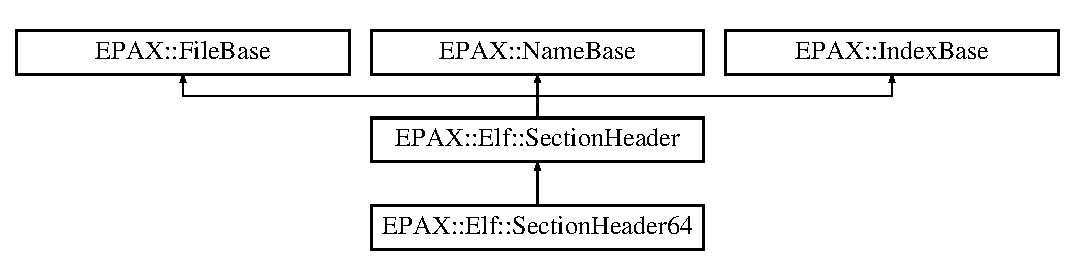
\includegraphics[height=3.000000cm]{class_e_p_a_x_1_1_elf_1_1_section_header64}
\end{center}
\end{figure}
\subsection*{\-Public \-Member \-Functions}
\begin{DoxyCompactItemize}
\item 
\hyperlink{class_e_p_a_x_1_1_elf_1_1_section_header64_a093e7ab0649ce9c396705d832b593018}{\-Section\-Header64} (\hyperlink{class_e_p_a_x_1_1_base_binary}{\-Base\-Binary} $\ast$b, uint64\-\_\-t o, uint64\-\_\-t s, uint32\-\_\-t i)
\item 
virtual \hyperlink{class_e_p_a_x_1_1_elf_1_1_section_header64_a4824e1c075af9b6939dfa2c67907979e}{$\sim$\-Section\-Header64} ()
\item 
uint64\-\_\-t \hyperlink{class_e_p_a_x_1_1_elf_1_1_section_header64_a4c83a831f07f96738a32fefd2f55b669}{get\-Name\-Index} ()
\item 
uint64\-\_\-t \hyperlink{class_e_p_a_x_1_1_elf_1_1_section_header64_a8556b692a71aba5e1048a7152cb1d837}{get\-Type} ()
\item 
uint64\-\_\-t \hyperlink{class_e_p_a_x_1_1_elf_1_1_section_header64_a5d82c8c6748a80bb0d53b8d6a6a9c3fb}{get\-Virt\-Addr} ()
\item 
uint64\-\_\-t \hyperlink{class_e_p_a_x_1_1_elf_1_1_section_header64_acd9363817d1fbab5194a3da55e8a7240}{get\-File\-Offset} ()
\item 
uint64\-\_\-t \hyperlink{class_e_p_a_x_1_1_elf_1_1_section_header64_aed1f49f68dc2b948fb8c5fe7d6df6ec5}{get\-Section\-Link} ()
\item 
uint64\-\_\-t \hyperlink{class_e_p_a_x_1_1_elf_1_1_section_header64_a8efa6c61a662689bd23732884b4a9aa5}{get\-Alignment} ()
\item 
uint64\-\_\-t \hyperlink{class_e_p_a_x_1_1_elf_1_1_section_header64_a3b16015c2864179254466fa389a5b90e}{get\-Entry\-Size} ()
\item 
uint64\-\_\-t \hyperlink{class_e_p_a_x_1_1_elf_1_1_section_header64_a4ca003bc2633ba8e16824a0d6f9f5dd1}{get\-Flags} ()
\item 
uint64\-\_\-t \hyperlink{class_e_p_a_x_1_1_elf_1_1_section_header64_a0b4f7cd68d065481a6953240f55f8073}{get\-Size} ()
\end{DoxyCompactItemize}


\subsection{\-Detailed \-Description}


\-Definition at line 302 of file \-Elf\-Binary.\-hpp.



\subsection{\-Constructor \& \-Destructor \-Documentation}
\hypertarget{class_e_p_a_x_1_1_elf_1_1_section_header64_a093e7ab0649ce9c396705d832b593018}{\index{\-E\-P\-A\-X\-::\-Elf\-::\-Section\-Header64@{\-E\-P\-A\-X\-::\-Elf\-::\-Section\-Header64}!\-Section\-Header64@{\-Section\-Header64}}
\index{\-Section\-Header64@{\-Section\-Header64}!EPAX::Elf::SectionHeader64@{\-E\-P\-A\-X\-::\-Elf\-::\-Section\-Header64}}
\subsubsection[{\-Section\-Header64}]{\setlength{\rightskip}{0pt plus 5cm}{\bf \-E\-P\-A\-X\-::\-Elf\-::\-Section\-Header64\-::\-Section\-Header64} (
\begin{DoxyParamCaption}
\item[{{\bf \-Base\-Binary} $\ast$}]{b, }
\item[{uint64\-\_\-t}]{o, }
\item[{uint64\-\_\-t}]{s, }
\item[{uint32\-\_\-t}]{i}
\end{DoxyParamCaption}
)}}\label{class_e_p_a_x_1_1_elf_1_1_section_header64_a093e7ab0649ce9c396705d832b593018}


\-Definition at line 794 of file \-Elf\-Binary.\-cpp.

\hypertarget{class_e_p_a_x_1_1_elf_1_1_section_header64_a4824e1c075af9b6939dfa2c67907979e}{\index{\-E\-P\-A\-X\-::\-Elf\-::\-Section\-Header64@{\-E\-P\-A\-X\-::\-Elf\-::\-Section\-Header64}!$\sim$\-Section\-Header64@{$\sim$\-Section\-Header64}}
\index{$\sim$\-Section\-Header64@{$\sim$\-Section\-Header64}!EPAX::Elf::SectionHeader64@{\-E\-P\-A\-X\-::\-Elf\-::\-Section\-Header64}}
\subsubsection[{$\sim$\-Section\-Header64}]{\setlength{\rightskip}{0pt plus 5cm}virtual {\bf \-E\-P\-A\-X\-::\-Elf\-::\-Section\-Header64\-::$\sim$\-Section\-Header64} (
\begin{DoxyParamCaption}
{}
\end{DoxyParamCaption}
)\hspace{0.3cm}{\ttfamily  \mbox{[}inline, virtual\mbox{]}}}}\label{class_e_p_a_x_1_1_elf_1_1_section_header64_a4824e1c075af9b6939dfa2c67907979e}


\-Definition at line 305 of file \-Elf\-Binary.\-hpp.



\subsection{\-Member \-Function \-Documentation}
\hypertarget{class_e_p_a_x_1_1_elf_1_1_section_header64_a8efa6c61a662689bd23732884b4a9aa5}{\index{\-E\-P\-A\-X\-::\-Elf\-::\-Section\-Header64@{\-E\-P\-A\-X\-::\-Elf\-::\-Section\-Header64}!get\-Alignment@{get\-Alignment}}
\index{get\-Alignment@{get\-Alignment}!EPAX::Elf::SectionHeader64@{\-E\-P\-A\-X\-::\-Elf\-::\-Section\-Header64}}
\subsubsection[{get\-Alignment}]{\setlength{\rightskip}{0pt plus 5cm}uint64\-\_\-t {\bf \-E\-P\-A\-X\-::\-Elf\-::\-Section\-Header64\-::get\-Alignment} (
\begin{DoxyParamCaption}
{}
\end{DoxyParamCaption}
)\hspace{0.3cm}{\ttfamily  \mbox{[}virtual\mbox{]}}}}\label{class_e_p_a_x_1_1_elf_1_1_section_header64_a8efa6c61a662689bd23732884b4a9aa5}


\-Implements \hyperlink{class_e_p_a_x_1_1_elf_1_1_section_header_a65a863f2eb15aa211d772fc1b3013d64}{\-E\-P\-A\-X\-::\-Elf\-::\-Section\-Header}.



\-Definition at line 853 of file \-Elf\-Binary.\-cpp.

\hypertarget{class_e_p_a_x_1_1_elf_1_1_section_header64_a3b16015c2864179254466fa389a5b90e}{\index{\-E\-P\-A\-X\-::\-Elf\-::\-Section\-Header64@{\-E\-P\-A\-X\-::\-Elf\-::\-Section\-Header64}!get\-Entry\-Size@{get\-Entry\-Size}}
\index{get\-Entry\-Size@{get\-Entry\-Size}!EPAX::Elf::SectionHeader64@{\-E\-P\-A\-X\-::\-Elf\-::\-Section\-Header64}}
\subsubsection[{get\-Entry\-Size}]{\setlength{\rightskip}{0pt plus 5cm}uint64\-\_\-t {\bf \-E\-P\-A\-X\-::\-Elf\-::\-Section\-Header64\-::get\-Entry\-Size} (
\begin{DoxyParamCaption}
{}
\end{DoxyParamCaption}
)\hspace{0.3cm}{\ttfamily  \mbox{[}virtual\mbox{]}}}}\label{class_e_p_a_x_1_1_elf_1_1_section_header64_a3b16015c2864179254466fa389a5b90e}


\-Implements \hyperlink{class_e_p_a_x_1_1_elf_1_1_section_header_a97327fc2deb88d4873bfa36b25864567}{\-E\-P\-A\-X\-::\-Elf\-::\-Section\-Header}.



\-Definition at line 861 of file \-Elf\-Binary.\-cpp.

\hypertarget{class_e_p_a_x_1_1_elf_1_1_section_header64_acd9363817d1fbab5194a3da55e8a7240}{\index{\-E\-P\-A\-X\-::\-Elf\-::\-Section\-Header64@{\-E\-P\-A\-X\-::\-Elf\-::\-Section\-Header64}!get\-File\-Offset@{get\-File\-Offset}}
\index{get\-File\-Offset@{get\-File\-Offset}!EPAX::Elf::SectionHeader64@{\-E\-P\-A\-X\-::\-Elf\-::\-Section\-Header64}}
\subsubsection[{get\-File\-Offset}]{\setlength{\rightskip}{0pt plus 5cm}uint64\-\_\-t {\bf \-E\-P\-A\-X\-::\-Elf\-::\-Section\-Header64\-::get\-File\-Offset} (
\begin{DoxyParamCaption}
{}
\end{DoxyParamCaption}
)\hspace{0.3cm}{\ttfamily  \mbox{[}virtual\mbox{]}}}}\label{class_e_p_a_x_1_1_elf_1_1_section_header64_acd9363817d1fbab5194a3da55e8a7240}


\-Implements \hyperlink{class_e_p_a_x_1_1_elf_1_1_section_header_a1beecb645d931ff31696e9994f1f0e06}{\-E\-P\-A\-X\-::\-Elf\-::\-Section\-Header}.



\-Definition at line 837 of file \-Elf\-Binary.\-cpp.

\hypertarget{class_e_p_a_x_1_1_elf_1_1_section_header64_a4ca003bc2633ba8e16824a0d6f9f5dd1}{\index{\-E\-P\-A\-X\-::\-Elf\-::\-Section\-Header64@{\-E\-P\-A\-X\-::\-Elf\-::\-Section\-Header64}!get\-Flags@{get\-Flags}}
\index{get\-Flags@{get\-Flags}!EPAX::Elf::SectionHeader64@{\-E\-P\-A\-X\-::\-Elf\-::\-Section\-Header64}}
\subsubsection[{get\-Flags}]{\setlength{\rightskip}{0pt plus 5cm}uint64\-\_\-t {\bf \-E\-P\-A\-X\-::\-Elf\-::\-Section\-Header64\-::get\-Flags} (
\begin{DoxyParamCaption}
{}
\end{DoxyParamCaption}
)\hspace{0.3cm}{\ttfamily  \mbox{[}virtual\mbox{]}}}}\label{class_e_p_a_x_1_1_elf_1_1_section_header64_a4ca003bc2633ba8e16824a0d6f9f5dd1}


\-Implements \hyperlink{class_e_p_a_x_1_1_elf_1_1_section_header_ab573a5f4b64afd5dc7f5b835c5b1becf}{\-E\-P\-A\-X\-::\-Elf\-::\-Section\-Header}.



\-Definition at line 869 of file \-Elf\-Binary.\-cpp.

\hypertarget{class_e_p_a_x_1_1_elf_1_1_section_header64_a4c83a831f07f96738a32fefd2f55b669}{\index{\-E\-P\-A\-X\-::\-Elf\-::\-Section\-Header64@{\-E\-P\-A\-X\-::\-Elf\-::\-Section\-Header64}!get\-Name\-Index@{get\-Name\-Index}}
\index{get\-Name\-Index@{get\-Name\-Index}!EPAX::Elf::SectionHeader64@{\-E\-P\-A\-X\-::\-Elf\-::\-Section\-Header64}}
\subsubsection[{get\-Name\-Index}]{\setlength{\rightskip}{0pt plus 5cm}uint64\-\_\-t {\bf \-E\-P\-A\-X\-::\-Elf\-::\-Section\-Header64\-::get\-Name\-Index} (
\begin{DoxyParamCaption}
{}
\end{DoxyParamCaption}
)\hspace{0.3cm}{\ttfamily  \mbox{[}virtual\mbox{]}}}}\label{class_e_p_a_x_1_1_elf_1_1_section_header64_a4c83a831f07f96738a32fefd2f55b669}


\-Implements \hyperlink{class_e_p_a_x_1_1_elf_1_1_section_header_aac92cdabd70a208e45ff0b6920bee3e6}{\-E\-P\-A\-X\-::\-Elf\-::\-Section\-Header}.



\-Definition at line 805 of file \-Elf\-Binary.\-cpp.

\hypertarget{class_e_p_a_x_1_1_elf_1_1_section_header64_aed1f49f68dc2b948fb8c5fe7d6df6ec5}{\index{\-E\-P\-A\-X\-::\-Elf\-::\-Section\-Header64@{\-E\-P\-A\-X\-::\-Elf\-::\-Section\-Header64}!get\-Section\-Link@{get\-Section\-Link}}
\index{get\-Section\-Link@{get\-Section\-Link}!EPAX::Elf::SectionHeader64@{\-E\-P\-A\-X\-::\-Elf\-::\-Section\-Header64}}
\subsubsection[{get\-Section\-Link}]{\setlength{\rightskip}{0pt plus 5cm}uint64\-\_\-t {\bf \-E\-P\-A\-X\-::\-Elf\-::\-Section\-Header64\-::get\-Section\-Link} (
\begin{DoxyParamCaption}
{}
\end{DoxyParamCaption}
)\hspace{0.3cm}{\ttfamily  \mbox{[}virtual\mbox{]}}}}\label{class_e_p_a_x_1_1_elf_1_1_section_header64_aed1f49f68dc2b948fb8c5fe7d6df6ec5}


\-Implements \hyperlink{class_e_p_a_x_1_1_elf_1_1_section_header_a035451e10f87faae8d772f8fda9e42d0}{\-E\-P\-A\-X\-::\-Elf\-::\-Section\-Header}.



\-Definition at line 845 of file \-Elf\-Binary.\-cpp.

\hypertarget{class_e_p_a_x_1_1_elf_1_1_section_header64_a0b4f7cd68d065481a6953240f55f8073}{\index{\-E\-P\-A\-X\-::\-Elf\-::\-Section\-Header64@{\-E\-P\-A\-X\-::\-Elf\-::\-Section\-Header64}!get\-Size@{get\-Size}}
\index{get\-Size@{get\-Size}!EPAX::Elf::SectionHeader64@{\-E\-P\-A\-X\-::\-Elf\-::\-Section\-Header64}}
\subsubsection[{get\-Size}]{\setlength{\rightskip}{0pt plus 5cm}uint64\-\_\-t {\bf \-E\-P\-A\-X\-::\-Elf\-::\-Section\-Header64\-::get\-Size} (
\begin{DoxyParamCaption}
{}
\end{DoxyParamCaption}
)\hspace{0.3cm}{\ttfamily  \mbox{[}virtual\mbox{]}}}}\label{class_e_p_a_x_1_1_elf_1_1_section_header64_a0b4f7cd68d065481a6953240f55f8073}


\-Implements \hyperlink{class_e_p_a_x_1_1_elf_1_1_section_header_a2d9cd842c34c4075260116f0ab373fa2}{\-E\-P\-A\-X\-::\-Elf\-::\-Section\-Header}.



\-Definition at line 821 of file \-Elf\-Binary.\-cpp.

\hypertarget{class_e_p_a_x_1_1_elf_1_1_section_header64_a8556b692a71aba5e1048a7152cb1d837}{\index{\-E\-P\-A\-X\-::\-Elf\-::\-Section\-Header64@{\-E\-P\-A\-X\-::\-Elf\-::\-Section\-Header64}!get\-Type@{get\-Type}}
\index{get\-Type@{get\-Type}!EPAX::Elf::SectionHeader64@{\-E\-P\-A\-X\-::\-Elf\-::\-Section\-Header64}}
\subsubsection[{get\-Type}]{\setlength{\rightskip}{0pt plus 5cm}uint64\-\_\-t {\bf \-E\-P\-A\-X\-::\-Elf\-::\-Section\-Header64\-::get\-Type} (
\begin{DoxyParamCaption}
{}
\end{DoxyParamCaption}
)\hspace{0.3cm}{\ttfamily  \mbox{[}virtual\mbox{]}}}}\label{class_e_p_a_x_1_1_elf_1_1_section_header64_a8556b692a71aba5e1048a7152cb1d837}


\-Implements \hyperlink{class_e_p_a_x_1_1_elf_1_1_section_header_af7e6230e8d4b68886ef8dcda238f1072}{\-E\-P\-A\-X\-::\-Elf\-::\-Section\-Header}.



\-Definition at line 813 of file \-Elf\-Binary.\-cpp.

\hypertarget{class_e_p_a_x_1_1_elf_1_1_section_header64_a5d82c8c6748a80bb0d53b8d6a6a9c3fb}{\index{\-E\-P\-A\-X\-::\-Elf\-::\-Section\-Header64@{\-E\-P\-A\-X\-::\-Elf\-::\-Section\-Header64}!get\-Virt\-Addr@{get\-Virt\-Addr}}
\index{get\-Virt\-Addr@{get\-Virt\-Addr}!EPAX::Elf::SectionHeader64@{\-E\-P\-A\-X\-::\-Elf\-::\-Section\-Header64}}
\subsubsection[{get\-Virt\-Addr}]{\setlength{\rightskip}{0pt plus 5cm}uint64\-\_\-t {\bf \-E\-P\-A\-X\-::\-Elf\-::\-Section\-Header64\-::get\-Virt\-Addr} (
\begin{DoxyParamCaption}
{}
\end{DoxyParamCaption}
)\hspace{0.3cm}{\ttfamily  \mbox{[}virtual\mbox{]}}}}\label{class_e_p_a_x_1_1_elf_1_1_section_header64_a5d82c8c6748a80bb0d53b8d6a6a9c3fb}


\-Implements \hyperlink{class_e_p_a_x_1_1_elf_1_1_section_header_a34bc5ee9fc05b1780e8cca68828bfc23}{\-E\-P\-A\-X\-::\-Elf\-::\-Section\-Header}.



\-Definition at line 829 of file \-Elf\-Binary.\-cpp.



\-The documentation for this class was generated from the following files\-:\begin{DoxyCompactItemize}
\item 
\hyperlink{_elf_binary_8hpp}{\-Elf\-Binary.\-hpp}\item 
\hyperlink{_elf_binary_8cpp}{\-Elf\-Binary.\-cpp}\end{DoxyCompactItemize}

\hypertarget{class_e_p_a_x_1_1_string_table}{\section{\-E\-P\-A\-X\-:\-:\-String\-Table \-Class \-Reference}
\label{class_e_p_a_x_1_1_string_table}\index{\-E\-P\-A\-X\-::\-String\-Table@{\-E\-P\-A\-X\-::\-String\-Table}}
}


{\ttfamily \#include $<$\-Symbol.\-hpp$>$}

\-Inheritance diagram for \-E\-P\-A\-X\-:\-:\-String\-Table\-:\begin{figure}[H]
\begin{center}
\leavevmode
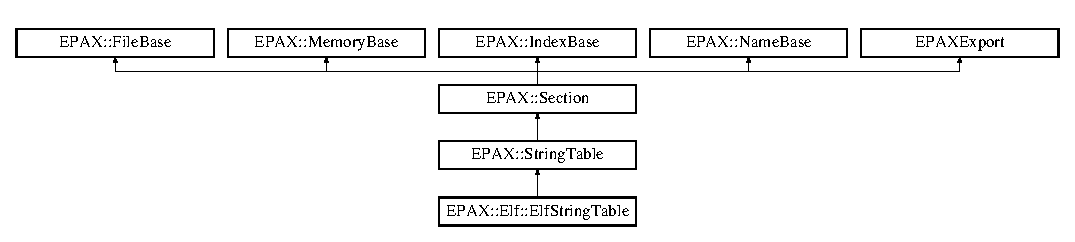
\includegraphics[height=2.800000cm]{class_e_p_a_x_1_1_string_table}
\end{center}
\end{figure}
\subsection*{\-Public \-Member \-Functions}
\begin{DoxyCompactItemize}
\item 
\hyperlink{class_e_p_a_x_1_1_string_table_a487cb8b4ce67da9743b6d8a2190aa7c8}{\-String\-Table} (\hyperlink{class_e_p_a_x_1_1_base_binary}{\-Base\-Binary} $\ast$b, uint64\-\_\-t o, uint64\-\_\-t fs, uint64\-\_\-t ma, uint64\-\_\-t ms, uint32\-\_\-t i, std\-::string n)
\item 
virtual \hyperlink{class_e_p_a_x_1_1_string_table_a7ac3b4fafdce508fed174efd5563b8b2}{$\sim$\-String\-Table} ()
\item 
virtual char $\ast$ \hyperlink{class_e_p_a_x_1_1_string_table_a1931cd14e2e3e1be340386f8bbbc6d2a}{get\-String\-At} (uint32\-\_\-t i)=0
\item 
bool \hyperlink{class_e_p_a_x_1_1_string_table_aef50a7eae11bd12b0c4ed93fff694c1d}{is\-String} ()
\end{DoxyCompactItemize}


\subsection{\-Detailed \-Description}


\-Definition at line 60 of file \-Symbol.\-hpp.



\subsection{\-Constructor \& \-Destructor \-Documentation}
\hypertarget{class_e_p_a_x_1_1_string_table_a487cb8b4ce67da9743b6d8a2190aa7c8}{\index{\-E\-P\-A\-X\-::\-String\-Table@{\-E\-P\-A\-X\-::\-String\-Table}!\-String\-Table@{\-String\-Table}}
\index{\-String\-Table@{\-String\-Table}!EPAX::StringTable@{\-E\-P\-A\-X\-::\-String\-Table}}
\subsubsection[{\-String\-Table}]{\setlength{\rightskip}{0pt plus 5cm}{\bf \-E\-P\-A\-X\-::\-String\-Table\-::\-String\-Table} (
\begin{DoxyParamCaption}
\item[{{\bf \-Base\-Binary} $\ast$}]{b, }
\item[{uint64\-\_\-t}]{o, }
\item[{uint64\-\_\-t}]{fs, }
\item[{uint64\-\_\-t}]{ma, }
\item[{uint64\-\_\-t}]{ms, }
\item[{uint32\-\_\-t}]{i, }
\item[{std\-::string}]{n}
\end{DoxyParamCaption}
)}}\label{class_e_p_a_x_1_1_string_table_a487cb8b4ce67da9743b6d8a2190aa7c8}


\-Definition at line 61 of file \-Symbol.\-cpp.

\hypertarget{class_e_p_a_x_1_1_string_table_a7ac3b4fafdce508fed174efd5563b8b2}{\index{\-E\-P\-A\-X\-::\-String\-Table@{\-E\-P\-A\-X\-::\-String\-Table}!$\sim$\-String\-Table@{$\sim$\-String\-Table}}
\index{$\sim$\-String\-Table@{$\sim$\-String\-Table}!EPAX::StringTable@{\-E\-P\-A\-X\-::\-String\-Table}}
\subsubsection[{$\sim$\-String\-Table}]{\setlength{\rightskip}{0pt plus 5cm}virtual {\bf \-E\-P\-A\-X\-::\-String\-Table\-::$\sim$\-String\-Table} (
\begin{DoxyParamCaption}
{}
\end{DoxyParamCaption}
)\hspace{0.3cm}{\ttfamily  \mbox{[}inline, virtual\mbox{]}}}}\label{class_e_p_a_x_1_1_string_table_a7ac3b4fafdce508fed174efd5563b8b2}


\-Definition at line 63 of file \-Symbol.\-hpp.



\subsection{\-Member \-Function \-Documentation}
\hypertarget{class_e_p_a_x_1_1_string_table_a1931cd14e2e3e1be340386f8bbbc6d2a}{\index{\-E\-P\-A\-X\-::\-String\-Table@{\-E\-P\-A\-X\-::\-String\-Table}!get\-String\-At@{get\-String\-At}}
\index{get\-String\-At@{get\-String\-At}!EPAX::StringTable@{\-E\-P\-A\-X\-::\-String\-Table}}
\subsubsection[{get\-String\-At}]{\setlength{\rightskip}{0pt plus 5cm}virtual char$\ast$ {\bf \-E\-P\-A\-X\-::\-String\-Table\-::get\-String\-At} (
\begin{DoxyParamCaption}
\item[{uint32\-\_\-t}]{i}
\end{DoxyParamCaption}
)\hspace{0.3cm}{\ttfamily  \mbox{[}pure virtual\mbox{]}}}}\label{class_e_p_a_x_1_1_string_table_a1931cd14e2e3e1be340386f8bbbc6d2a}


\-Implemented in \hyperlink{class_e_p_a_x_1_1_elf_1_1_elf_string_table_a5090981e577dceb27e8dd6c63f1992ba}{\-E\-P\-A\-X\-::\-Elf\-::\-Elf\-String\-Table}.

\hypertarget{class_e_p_a_x_1_1_string_table_aef50a7eae11bd12b0c4ed93fff694c1d}{\index{\-E\-P\-A\-X\-::\-String\-Table@{\-E\-P\-A\-X\-::\-String\-Table}!is\-String@{is\-String}}
\index{is\-String@{is\-String}!EPAX::StringTable@{\-E\-P\-A\-X\-::\-String\-Table}}
\subsubsection[{is\-String}]{\setlength{\rightskip}{0pt plus 5cm}bool {\bf \-E\-P\-A\-X\-::\-String\-Table\-::is\-String} (
\begin{DoxyParamCaption}
{}
\end{DoxyParamCaption}
)\hspace{0.3cm}{\ttfamily  \mbox{[}inline, virtual\mbox{]}}}}\label{class_e_p_a_x_1_1_string_table_aef50a7eae11bd12b0c4ed93fff694c1d}


\-Reimplemented from \hyperlink{class_e_p_a_x_1_1_section_a04c811caf98179122fa6443095bde52d}{\-E\-P\-A\-X\-::\-Section}.



\-Definition at line 67 of file \-Symbol.\-hpp.



\-The documentation for this class was generated from the following files\-:\begin{DoxyCompactItemize}
\item 
\hyperlink{_symbol_8hpp}{\-Symbol.\-hpp}\item 
\hyperlink{_symbol_8cpp}{\-Symbol.\-cpp}\end{DoxyCompactItemize}

\hypertarget{class_e_p_a_x_1_1_symbol}{\section{\-E\-P\-A\-X\-:\-:\-Symbol \-Class \-Reference}
\label{class_e_p_a_x_1_1_symbol}\index{\-E\-P\-A\-X\-::\-Symbol@{\-E\-P\-A\-X\-::\-Symbol}}
}


{\ttfamily \#include $<$\-Symbol.\-hpp$>$}

\-Inheritance diagram for \-E\-P\-A\-X\-:\-:\-Symbol\-:\begin{figure}[H]
\begin{center}
\leavevmode
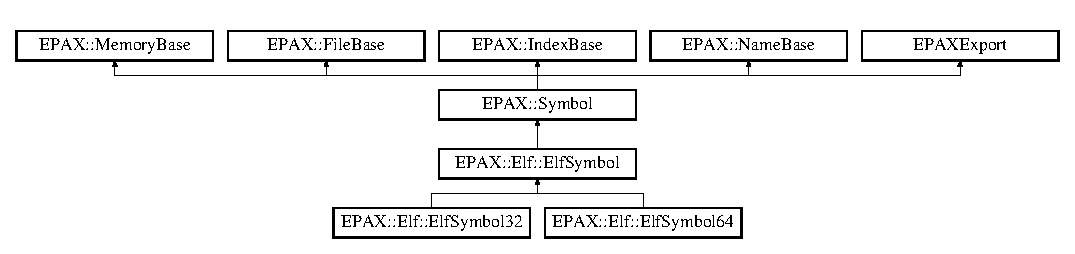
\includegraphics[height=2.966887cm]{class_e_p_a_x_1_1_symbol}
\end{center}
\end{figure}
\subsection*{\-Public \-Member \-Functions}
\begin{DoxyCompactItemize}
\item 
\hyperlink{class_e_p_a_x_1_1_symbol_a4d1c4e92f875293df6903aeb01b7be3f}{\-Symbol} (\hyperlink{class_e_p_a_x_1_1_base_binary}{\-Base\-Binary} $\ast$b, uint64\-\_\-t o, uint64\-\_\-t s, uint32\-\_\-t i)
\item 
virtual \hyperlink{class_e_p_a_x_1_1_symbol_ae0bd01bf034fe2209cfcea1054d04ded}{$\sim$\-Symbol} ()
\item 
virtual bool \hyperlink{class_e_p_a_x_1_1_symbol_a1dc3c27cb8debeda55cad9d3e04a7be5}{is\-Function} ()=0
\item 
virtual bool \hyperlink{class_e_p_a_x_1_1_symbol_a58d8007f908063fc4602c042a739bd8f}{is\-Thumb\-Function} ()=0
\end{DoxyCompactItemize}


\subsection{\-Detailed \-Description}


\-Definition at line 35 of file \-Symbol.\-hpp.



\subsection{\-Constructor \& \-Destructor \-Documentation}
\hypertarget{class_e_p_a_x_1_1_symbol_a4d1c4e92f875293df6903aeb01b7be3f}{\index{\-E\-P\-A\-X\-::\-Symbol@{\-E\-P\-A\-X\-::\-Symbol}!\-Symbol@{\-Symbol}}
\index{\-Symbol@{\-Symbol}!EPAX::Symbol@{\-E\-P\-A\-X\-::\-Symbol}}
\subsubsection[{\-Symbol}]{\setlength{\rightskip}{0pt plus 5cm}{\bf \-E\-P\-A\-X\-::\-Symbol\-::\-Symbol} (
\begin{DoxyParamCaption}
\item[{{\bf \-Base\-Binary} $\ast$}]{b, }
\item[{uint64\-\_\-t}]{o, }
\item[{uint64\-\_\-t}]{s, }
\item[{uint32\-\_\-t}]{i}
\end{DoxyParamCaption}
)}}\label{class_e_p_a_x_1_1_symbol_a4d1c4e92f875293df6903aeb01b7be3f}


\-Definition at line 31 of file \-Symbol.\-cpp.

\hypertarget{class_e_p_a_x_1_1_symbol_ae0bd01bf034fe2209cfcea1054d04ded}{\index{\-E\-P\-A\-X\-::\-Symbol@{\-E\-P\-A\-X\-::\-Symbol}!$\sim$\-Symbol@{$\sim$\-Symbol}}
\index{$\sim$\-Symbol@{$\sim$\-Symbol}!EPAX::Symbol@{\-E\-P\-A\-X\-::\-Symbol}}
\subsubsection[{$\sim$\-Symbol}]{\setlength{\rightskip}{0pt plus 5cm}virtual {\bf \-E\-P\-A\-X\-::\-Symbol\-::$\sim$\-Symbol} (
\begin{DoxyParamCaption}
{}
\end{DoxyParamCaption}
)\hspace{0.3cm}{\ttfamily  \mbox{[}inline, virtual\mbox{]}}}}\label{class_e_p_a_x_1_1_symbol_ae0bd01bf034fe2209cfcea1054d04ded}


\-Definition at line 38 of file \-Symbol.\-hpp.



\subsection{\-Member \-Function \-Documentation}
\hypertarget{class_e_p_a_x_1_1_symbol_a1dc3c27cb8debeda55cad9d3e04a7be5}{\index{\-E\-P\-A\-X\-::\-Symbol@{\-E\-P\-A\-X\-::\-Symbol}!is\-Function@{is\-Function}}
\index{is\-Function@{is\-Function}!EPAX::Symbol@{\-E\-P\-A\-X\-::\-Symbol}}
\subsubsection[{is\-Function}]{\setlength{\rightskip}{0pt plus 5cm}virtual bool {\bf \-E\-P\-A\-X\-::\-Symbol\-::is\-Function} (
\begin{DoxyParamCaption}
{}
\end{DoxyParamCaption}
)\hspace{0.3cm}{\ttfamily  \mbox{[}pure virtual\mbox{]}}}}\label{class_e_p_a_x_1_1_symbol_a1dc3c27cb8debeda55cad9d3e04a7be5}


\-Implemented in \hyperlink{class_e_p_a_x_1_1_elf_1_1_elf_symbol_ad6142f5f07372bffd2f0b9a482696821}{\-E\-P\-A\-X\-::\-Elf\-::\-Elf\-Symbol}.

\hypertarget{class_e_p_a_x_1_1_symbol_a58d8007f908063fc4602c042a739bd8f}{\index{\-E\-P\-A\-X\-::\-Symbol@{\-E\-P\-A\-X\-::\-Symbol}!is\-Thumb\-Function@{is\-Thumb\-Function}}
\index{is\-Thumb\-Function@{is\-Thumb\-Function}!EPAX::Symbol@{\-E\-P\-A\-X\-::\-Symbol}}
\subsubsection[{is\-Thumb\-Function}]{\setlength{\rightskip}{0pt plus 5cm}virtual bool {\bf \-E\-P\-A\-X\-::\-Symbol\-::is\-Thumb\-Function} (
\begin{DoxyParamCaption}
{}
\end{DoxyParamCaption}
)\hspace{0.3cm}{\ttfamily  \mbox{[}pure virtual\mbox{]}}}}\label{class_e_p_a_x_1_1_symbol_a58d8007f908063fc4602c042a739bd8f}


\-Implemented in \hyperlink{class_e_p_a_x_1_1_elf_1_1_elf_symbol_a4f27b2be55f35a4c9a75b5e52bce6e23}{\-E\-P\-A\-X\-::\-Elf\-::\-Elf\-Symbol}.



\-The documentation for this class was generated from the following files\-:\begin{DoxyCompactItemize}
\item 
\hyperlink{_symbol_8hpp}{\-Symbol.\-hpp}\item 
\hyperlink{_symbol_8cpp}{\-Symbol.\-cpp}\end{DoxyCompactItemize}

\hypertarget{class_e_p_a_x_1_1_symbol_base}{\section{\-E\-P\-A\-X\-:\-:\-Symbol\-Base \-Class \-Reference}
\label{class_e_p_a_x_1_1_symbol_base}\index{\-E\-P\-A\-X\-::\-Symbol\-Base@{\-E\-P\-A\-X\-::\-Symbol\-Base}}
}


{\ttfamily \#include $<$\-Base\-Class.\-hpp$>$}

\-Inheritance diagram for \-E\-P\-A\-X\-:\-:\-Symbol\-Base\-:\begin{figure}[H]
\begin{center}
\leavevmode
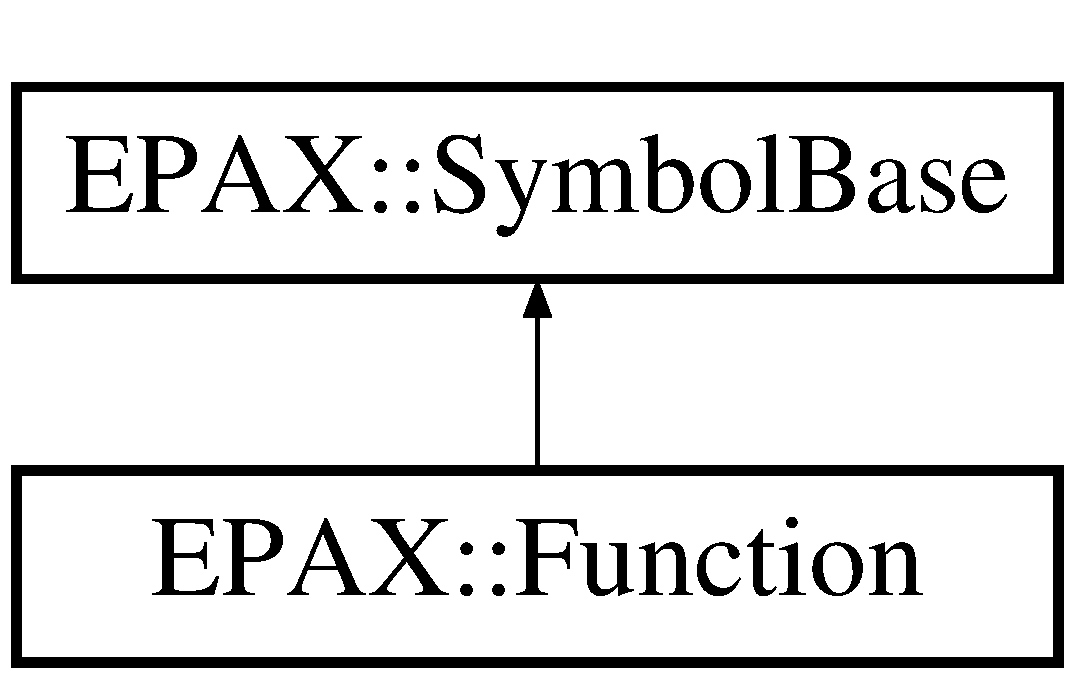
\includegraphics[height=2.000000cm]{class_e_p_a_x_1_1_symbol_base}
\end{center}
\end{figure}
\subsection*{\-Public \-Member \-Functions}
\begin{DoxyCompactItemize}
\item 
\hyperlink{class_e_p_a_x_1_1_symbol_base_a8f9eba0867c5b241168ee2efd929a6b9}{\-Symbol\-Base} (\hyperlink{class_e_p_a_x_1_1_symbol}{\-Symbol} $\ast$s)
\item 
virtual \hyperlink{class_e_p_a_x_1_1_symbol_base_ae2793fb63d87e3437b77ac5d35258355}{$\sim$\-Symbol\-Base} ()
\item 
\hyperlink{class_e_p_a_x_1_1_symbol}{\-Symbol} $\ast$ \hyperlink{class_e_p_a_x_1_1_symbol_base_aab5102b6c977d0e2572dbbc6d182ae00}{get\-Symbol} ()
\item 
void \hyperlink{class_e_p_a_x_1_1_symbol_base_a2d946999ece0fc16721586357067888b}{set\-Symbol} (\hyperlink{class_e_p_a_x_1_1_symbol}{\-Symbol} $\ast$s)
\item 
std\-::string \hyperlink{class_e_p_a_x_1_1_symbol_base_a85ec412485a26fa166523f3dc0b3fbf2}{get\-Name} ()
\end{DoxyCompactItemize}


\subsection{\-Detailed \-Description}


\-Definition at line 80 of file \-Base\-Class.\-hpp.



\subsection{\-Constructor \& \-Destructor \-Documentation}
\hypertarget{class_e_p_a_x_1_1_symbol_base_a8f9eba0867c5b241168ee2efd929a6b9}{\index{\-E\-P\-A\-X\-::\-Symbol\-Base@{\-E\-P\-A\-X\-::\-Symbol\-Base}!\-Symbol\-Base@{\-Symbol\-Base}}
\index{\-Symbol\-Base@{\-Symbol\-Base}!EPAX::SymbolBase@{\-E\-P\-A\-X\-::\-Symbol\-Base}}
\subsubsection[{\-Symbol\-Base}]{\setlength{\rightskip}{0pt plus 5cm}{\bf \-E\-P\-A\-X\-::\-Symbol\-Base\-::\-Symbol\-Base} (
\begin{DoxyParamCaption}
\item[{{\bf \-Symbol} $\ast$}]{s}
\end{DoxyParamCaption}
)\hspace{0.3cm}{\ttfamily  \mbox{[}inline\mbox{]}}}}\label{class_e_p_a_x_1_1_symbol_base_a8f9eba0867c5b241168ee2efd929a6b9}


\-Definition at line 84 of file \-Base\-Class.\-hpp.

\hypertarget{class_e_p_a_x_1_1_symbol_base_ae2793fb63d87e3437b77ac5d35258355}{\index{\-E\-P\-A\-X\-::\-Symbol\-Base@{\-E\-P\-A\-X\-::\-Symbol\-Base}!$\sim$\-Symbol\-Base@{$\sim$\-Symbol\-Base}}
\index{$\sim$\-Symbol\-Base@{$\sim$\-Symbol\-Base}!EPAX::SymbolBase@{\-E\-P\-A\-X\-::\-Symbol\-Base}}
\subsubsection[{$\sim$\-Symbol\-Base}]{\setlength{\rightskip}{0pt plus 5cm}virtual {\bf \-E\-P\-A\-X\-::\-Symbol\-Base\-::$\sim$\-Symbol\-Base} (
\begin{DoxyParamCaption}
{}
\end{DoxyParamCaption}
)\hspace{0.3cm}{\ttfamily  \mbox{[}inline, virtual\mbox{]}}}}\label{class_e_p_a_x_1_1_symbol_base_ae2793fb63d87e3437b77ac5d35258355}


\-Definition at line 86 of file \-Base\-Class.\-hpp.



\subsection{\-Member \-Function \-Documentation}
\hypertarget{class_e_p_a_x_1_1_symbol_base_a85ec412485a26fa166523f3dc0b3fbf2}{\index{\-E\-P\-A\-X\-::\-Symbol\-Base@{\-E\-P\-A\-X\-::\-Symbol\-Base}!get\-Name@{get\-Name}}
\index{get\-Name@{get\-Name}!EPAX::SymbolBase@{\-E\-P\-A\-X\-::\-Symbol\-Base}}
\subsubsection[{get\-Name}]{\setlength{\rightskip}{0pt plus 5cm}std\-::string {\bf \-E\-P\-A\-X\-::\-Symbol\-Base\-::get\-Name} (
\begin{DoxyParamCaption}
{}
\end{DoxyParamCaption}
)}}\label{class_e_p_a_x_1_1_symbol_base_a85ec412485a26fa166523f3dc0b3fbf2}


\-Definition at line 39 of file \-Base\-Class.\-cpp.

\hypertarget{class_e_p_a_x_1_1_symbol_base_aab5102b6c977d0e2572dbbc6d182ae00}{\index{\-E\-P\-A\-X\-::\-Symbol\-Base@{\-E\-P\-A\-X\-::\-Symbol\-Base}!get\-Symbol@{get\-Symbol}}
\index{get\-Symbol@{get\-Symbol}!EPAX::SymbolBase@{\-E\-P\-A\-X\-::\-Symbol\-Base}}
\subsubsection[{get\-Symbol}]{\setlength{\rightskip}{0pt plus 5cm}{\bf \-Symbol}$\ast$ {\bf \-E\-P\-A\-X\-::\-Symbol\-Base\-::get\-Symbol} (
\begin{DoxyParamCaption}
{}
\end{DoxyParamCaption}
)\hspace{0.3cm}{\ttfamily  \mbox{[}inline\mbox{]}}}}\label{class_e_p_a_x_1_1_symbol_base_aab5102b6c977d0e2572dbbc6d182ae00}


\-Definition at line 88 of file \-Base\-Class.\-hpp.

\hypertarget{class_e_p_a_x_1_1_symbol_base_a2d946999ece0fc16721586357067888b}{\index{\-E\-P\-A\-X\-::\-Symbol\-Base@{\-E\-P\-A\-X\-::\-Symbol\-Base}!set\-Symbol@{set\-Symbol}}
\index{set\-Symbol@{set\-Symbol}!EPAX::SymbolBase@{\-E\-P\-A\-X\-::\-Symbol\-Base}}
\subsubsection[{set\-Symbol}]{\setlength{\rightskip}{0pt plus 5cm}void {\bf \-E\-P\-A\-X\-::\-Symbol\-Base\-::set\-Symbol} (
\begin{DoxyParamCaption}
\item[{{\bf \-Symbol} $\ast$}]{s}
\end{DoxyParamCaption}
)\hspace{0.3cm}{\ttfamily  \mbox{[}inline\mbox{]}}}}\label{class_e_p_a_x_1_1_symbol_base_a2d946999ece0fc16721586357067888b}


\-Definition at line 89 of file \-Base\-Class.\-hpp.



\-The documentation for this class was generated from the following files\-:\begin{DoxyCompactItemize}
\item 
\hyperlink{_base_class_8hpp}{\-Base\-Class.\-hpp}\item 
\hyperlink{_base_class_8cpp}{\-Base\-Class.\-cpp}\end{DoxyCompactItemize}

\hypertarget{class_e_p_a_x_1_1_symbol_table}{\section{\-E\-P\-A\-X\-:\-:\-Symbol\-Table \-Class \-Reference}
\label{class_e_p_a_x_1_1_symbol_table}\index{\-E\-P\-A\-X\-::\-Symbol\-Table@{\-E\-P\-A\-X\-::\-Symbol\-Table}}
}


{\ttfamily \#include $<$\-Symbol.\-hpp$>$}

\-Inheritance diagram for \-E\-P\-A\-X\-:\-:\-Symbol\-Table\-:\begin{figure}[H]
\begin{center}
\leavevmode
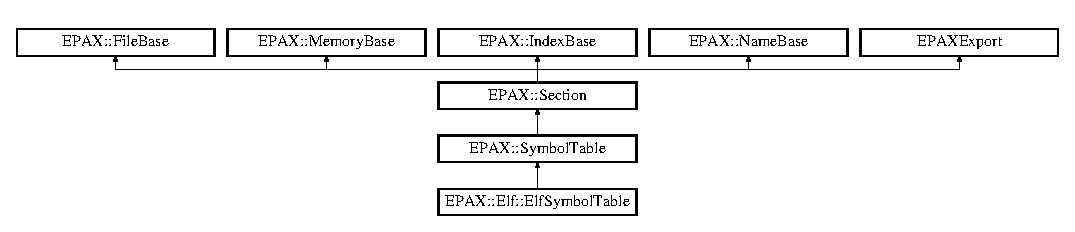
\includegraphics[height=2.666667cm]{class_e_p_a_x_1_1_symbol_table}
\end{center}
\end{figure}
\subsection*{\-Public \-Member \-Functions}
\begin{DoxyCompactItemize}
\item 
\hyperlink{class_e_p_a_x_1_1_symbol_table_a5a287e768e39c5bbb7325a5039c5569f}{\-Symbol\-Table} (\hyperlink{class_e_p_a_x_1_1_base_binary}{\-Base\-Binary} $\ast$b, uint64\-\_\-t o, uint64\-\_\-t fs, uint64\-\_\-t ma, uint64\-\_\-t ms, uint32\-\_\-t i, std\-::string n)
\item 
virtual \hyperlink{class_e_p_a_x_1_1_symbol_table_a97d8c6f6517b3ae2ea39f0c47dd60a5b}{$\sim$\-Symbol\-Table} ()
\item 
uint32\-\_\-t \hyperlink{class_e_p_a_x_1_1_symbol_table_a229729af626ddb0763a1bff287b68918}{count\-Symbols} ()
\item 
\hyperlink{class_e_p_a_x_1_1_symbol}{\-Symbol} $\ast$ \hyperlink{class_e_p_a_x_1_1_symbol_table_a6a4a90088e81ef66cf665c241b9fa1f0}{get\-Symbol} (uint32\-\_\-t i)
\item 
virtual void \hyperlink{class_e_p_a_x_1_1_symbol_table_ac8a581679e678f1472bf684fdf877b9a}{print} (std\-::ostream \&stream=std\-::cout)=0
\item 
bool \hyperlink{class_e_p_a_x_1_1_symbol_table_a86c210d632debcae293bd2167a3cbe62}{is\-Symbol} ()
\end{DoxyCompactItemize}
\subsection*{\-Protected \-Attributes}
\begin{DoxyCompactItemize}
\item 
std\-::vector$<$ \hyperlink{class_e_p_a_x_1_1_symbol}{\-Symbol} $\ast$ $>$ $\ast$ \hyperlink{class_e_p_a_x_1_1_symbol_table_ae9f0215b62e323d3edecd86fddae58c2}{symbols}
\end{DoxyCompactItemize}


\subsection{\-Detailed \-Description}


\-Definition at line 44 of file \-Symbol.\-hpp.



\subsection{\-Constructor \& \-Destructor \-Documentation}
\hypertarget{class_e_p_a_x_1_1_symbol_table_a5a287e768e39c5bbb7325a5039c5569f}{\index{\-E\-P\-A\-X\-::\-Symbol\-Table@{\-E\-P\-A\-X\-::\-Symbol\-Table}!\-Symbol\-Table@{\-Symbol\-Table}}
\index{\-Symbol\-Table@{\-Symbol\-Table}!EPAX::SymbolTable@{\-E\-P\-A\-X\-::\-Symbol\-Table}}
\subsubsection[{\-Symbol\-Table}]{\setlength{\rightskip}{0pt plus 5cm}{\bf \-E\-P\-A\-X\-::\-Symbol\-Table\-::\-Symbol\-Table} (
\begin{DoxyParamCaption}
\item[{{\bf \-Base\-Binary} $\ast$}]{b, }
\item[{uint64\-\_\-t}]{o, }
\item[{uint64\-\_\-t}]{fs, }
\item[{uint64\-\_\-t}]{ma, }
\item[{uint64\-\_\-t}]{ms, }
\item[{uint32\-\_\-t}]{i, }
\item[{std\-::string}]{n}
\end{DoxyParamCaption}
)}}\label{class_e_p_a_x_1_1_symbol_table_a5a287e768e39c5bbb7325a5039c5569f}


\-Definition at line 40 of file \-Symbol.\-cpp.

\hypertarget{class_e_p_a_x_1_1_symbol_table_a97d8c6f6517b3ae2ea39f0c47dd60a5b}{\index{\-E\-P\-A\-X\-::\-Symbol\-Table@{\-E\-P\-A\-X\-::\-Symbol\-Table}!$\sim$\-Symbol\-Table@{$\sim$\-Symbol\-Table}}
\index{$\sim$\-Symbol\-Table@{$\sim$\-Symbol\-Table}!EPAX::SymbolTable@{\-E\-P\-A\-X\-::\-Symbol\-Table}}
\subsubsection[{$\sim$\-Symbol\-Table}]{\setlength{\rightskip}{0pt plus 5cm}{\bf \-E\-P\-A\-X\-::\-Symbol\-Table\-::$\sim$\-Symbol\-Table} (
\begin{DoxyParamCaption}
{}
\end{DoxyParamCaption}
)\hspace{0.3cm}{\ttfamily  \mbox{[}virtual\mbox{]}}}}\label{class_e_p_a_x_1_1_symbol_table_a97d8c6f6517b3ae2ea39f0c47dd60a5b}


\-Definition at line 46 of file \-Symbol.\-cpp.



\subsection{\-Member \-Function \-Documentation}
\hypertarget{class_e_p_a_x_1_1_symbol_table_a229729af626ddb0763a1bff287b68918}{\index{\-E\-P\-A\-X\-::\-Symbol\-Table@{\-E\-P\-A\-X\-::\-Symbol\-Table}!count\-Symbols@{count\-Symbols}}
\index{count\-Symbols@{count\-Symbols}!EPAX::SymbolTable@{\-E\-P\-A\-X\-::\-Symbol\-Table}}
\subsubsection[{count\-Symbols}]{\setlength{\rightskip}{0pt plus 5cm}uint32\-\_\-t {\bf \-E\-P\-A\-X\-::\-Symbol\-Table\-::count\-Symbols} (
\begin{DoxyParamCaption}
{}
\end{DoxyParamCaption}
)\hspace{0.3cm}{\ttfamily  \mbox{[}inline\mbox{]}}}}\label{class_e_p_a_x_1_1_symbol_table_a229729af626ddb0763a1bff287b68918}


\-Definition at line 52 of file \-Symbol.\-hpp.

\hypertarget{class_e_p_a_x_1_1_symbol_table_a6a4a90088e81ef66cf665c241b9fa1f0}{\index{\-E\-P\-A\-X\-::\-Symbol\-Table@{\-E\-P\-A\-X\-::\-Symbol\-Table}!get\-Symbol@{get\-Symbol}}
\index{get\-Symbol@{get\-Symbol}!EPAX::SymbolTable@{\-E\-P\-A\-X\-::\-Symbol\-Table}}
\subsubsection[{get\-Symbol}]{\setlength{\rightskip}{0pt plus 5cm}{\bf \-Symbol} $\ast$ {\bf \-E\-P\-A\-X\-::\-Symbol\-Table\-::get\-Symbol} (
\begin{DoxyParamCaption}
\item[{uint32\-\_\-t}]{i}
\end{DoxyParamCaption}
)}}\label{class_e_p_a_x_1_1_symbol_table_a6a4a90088e81ef66cf665c241b9fa1f0}


\-Definition at line 56 of file \-Symbol.\-cpp.

\hypertarget{class_e_p_a_x_1_1_symbol_table_a86c210d632debcae293bd2167a3cbe62}{\index{\-E\-P\-A\-X\-::\-Symbol\-Table@{\-E\-P\-A\-X\-::\-Symbol\-Table}!is\-Symbol@{is\-Symbol}}
\index{is\-Symbol@{is\-Symbol}!EPAX::SymbolTable@{\-E\-P\-A\-X\-::\-Symbol\-Table}}
\subsubsection[{is\-Symbol}]{\setlength{\rightskip}{0pt plus 5cm}bool {\bf \-E\-P\-A\-X\-::\-Symbol\-Table\-::is\-Symbol} (
\begin{DoxyParamCaption}
{}
\end{DoxyParamCaption}
)\hspace{0.3cm}{\ttfamily  \mbox{[}inline, virtual\mbox{]}}}}\label{class_e_p_a_x_1_1_symbol_table_a86c210d632debcae293bd2167a3cbe62}


\-Reimplemented from \hyperlink{class_e_p_a_x_1_1_section_a6f8fdba06c4f3506d4dc2df97658157f}{\-E\-P\-A\-X\-::\-Section}.



\-Definition at line 57 of file \-Symbol.\-hpp.

\hypertarget{class_e_p_a_x_1_1_symbol_table_ac8a581679e678f1472bf684fdf877b9a}{\index{\-E\-P\-A\-X\-::\-Symbol\-Table@{\-E\-P\-A\-X\-::\-Symbol\-Table}!print@{print}}
\index{print@{print}!EPAX::SymbolTable@{\-E\-P\-A\-X\-::\-Symbol\-Table}}
\subsubsection[{print}]{\setlength{\rightskip}{0pt plus 5cm}virtual void {\bf \-E\-P\-A\-X\-::\-Symbol\-Table\-::print} (
\begin{DoxyParamCaption}
\item[{std\-::ostream \&}]{stream = {\ttfamily std\-:\-:cout}}
\end{DoxyParamCaption}
)\hspace{0.3cm}{\ttfamily  \mbox{[}pure virtual\mbox{]}}}}\label{class_e_p_a_x_1_1_symbol_table_ac8a581679e678f1472bf684fdf877b9a}


\-Reimplemented from \hyperlink{class_e_p_a_x_1_1_section_ad79a91be22efd4499b78d2554ebc8285}{\-E\-P\-A\-X\-::\-Section}.



\-Implemented in \hyperlink{class_e_p_a_x_1_1_elf_1_1_elf_symbol_table_af8c0bb17c3b8c38ee49142def9ee0ed0}{\-E\-P\-A\-X\-::\-Elf\-::\-Elf\-Symbol\-Table}.



\subsection{\-Member \-Data \-Documentation}
\hypertarget{class_e_p_a_x_1_1_symbol_table_ae9f0215b62e323d3edecd86fddae58c2}{\index{\-E\-P\-A\-X\-::\-Symbol\-Table@{\-E\-P\-A\-X\-::\-Symbol\-Table}!symbols@{symbols}}
\index{symbols@{symbols}!EPAX::SymbolTable@{\-E\-P\-A\-X\-::\-Symbol\-Table}}
\subsubsection[{symbols}]{\setlength{\rightskip}{0pt plus 5cm}std\-::vector$<${\bf \-Symbol}$\ast$$>$$\ast$ {\bf \-E\-P\-A\-X\-::\-Symbol\-Table\-::symbols}\hspace{0.3cm}{\ttfamily  \mbox{[}protected\mbox{]}}}}\label{class_e_p_a_x_1_1_symbol_table_ae9f0215b62e323d3edecd86fddae58c2}


\-Definition at line 46 of file \-Symbol.\-hpp.



\-The documentation for this class was generated from the following files\-:\begin{DoxyCompactItemize}
\item 
\hyperlink{_symbol_8hpp}{\-Symbol.\-hpp}\item 
\hyperlink{_symbol_8cpp}{\-Symbol.\-cpp}\end{DoxyCompactItemize}

\chapter{\-File \-Documentation}
\hypertarget{_base_class_8cpp}{\section{\-Base\-Class.\-cpp \-File \-Reference}
\label{_base_class_8cpp}\index{\-Base\-Class.\-cpp@{\-Base\-Class.\-cpp}}
}
{\ttfamily \#include \char`\"{}\-E\-P\-A\-X\-Common\-Internal.\-hpp\char`\"{}}\*
{\ttfamily \#include \char`\"{}\-Base\-Class.\-hpp\char`\"{}}\*
{\ttfamily \#include \char`\"{}\-Input\-File.\-hpp\char`\"{}}\*
{\ttfamily \#include \char`\"{}\-Function.\-hpp\char`\"{}}\*
{\ttfamily \#include \char`\"{}\-Symbol.\-hpp\char`\"{}}\*
{\ttfamily \#include \char`\"{}\-Section.\-hpp\char`\"{}}\*
\subsection*{\-Namespaces}
\begin{DoxyCompactItemize}
\item 
namespace \hyperlink{namespace_e_p_a_x}{\-E\-P\-A\-X}
\end{DoxyCompactItemize}
\subsection*{\-Functions}
\begin{DoxyCompactItemize}
\item 
bool \hyperlink{namespace_e_p_a_x_aef55d3382820337f1f2759dca145b428}{\-E\-P\-A\-X\-::compare\-Memory} (\-Memory\-Base $\ast$m1, \-Memory\-Base $\ast$m2)
\end{DoxyCompactItemize}


\subsection{\-Detailed \-Description}
\hypertarget{_symbol_8hpp_LICENSE}{}\subsection{\-L\-I\-C\-E\-N\-S\-E}\label{_symbol_8hpp_LICENSE}
\-This file is part of the \hyperlink{namespace_e_p_a_x}{\-E\-P\-A\-X} toolkit.

\-Copyright (c) 2013, \-E\-P \-Analytics, \-Inc. \-All rights reserved.

\-This program is free software\-: you can redistribute it and/or modify it under the terms of the \-G\-N\-U \-General \-Public \-License as published by the \-Free \-Software \-Foundation, either version 3 of the \-License, or (at your option) any later version.

\-This program is distributed in the hope that it will be useful, but \-W\-I\-T\-H\-O\-U\-T \-A\-N\-Y \-W\-A\-R\-R\-A\-N\-T\-Y; without even the implied warranty of \-M\-E\-R\-C\-H\-A\-N\-T\-A\-B\-I\-L\-I\-T\-Y or \-F\-I\-T\-N\-E\-S\-S \-F\-O\-R \-A \-P\-A\-R\-T\-I\-C\-U\-L\-A\-R \-P\-U\-R\-P\-O\-S\-E. \-See the \-G\-N\-U \-General \-Public \-License for more details.

\-You should have received a copy of the \-G\-N\-U \-General \-Public \-License along with this program. \-If not, see $<$\href{http://www.gnu.org/licenses/}{\tt http\-://www.\-gnu.\-org/licenses/}$>$. 

\-Definition in file \hyperlink{_base_class_8cpp_source}{\-Base\-Class.\-cpp}.


\hypertarget{_base_class_8hpp}{\section{\-Base\-Class.\-hpp \-File \-Reference}
\label{_base_class_8hpp}\index{\-Base\-Class.\-hpp@{\-Base\-Class.\-hpp}}
}
{\ttfamily \#include \char`\"{}\-Binary.\-hpp\char`\"{}}\*
\subsection*{\-Classes}
\begin{DoxyCompactItemize}
\item 
class \hyperlink{class_e_p_a_x_1_1_file_base}{\-E\-P\-A\-X\-::\-File\-Base}
\item 
class \hyperlink{class_e_p_a_x_1_1_memory_base}{\-E\-P\-A\-X\-::\-Memory\-Base}
\item 
class \hyperlink{class_e_p_a_x_1_1_symbol_base}{\-E\-P\-A\-X\-::\-Symbol\-Base}
\item 
class \hyperlink{class_e_p_a_x_1_1_index_base}{\-E\-P\-A\-X\-::\-Index\-Base}
\item 
class \hyperlink{class_e_p_a_x_1_1_name_base}{\-E\-P\-A\-X\-::\-Name\-Base}
\item 
class \hyperlink{class_e_p_a_x_1_1_base_binary}{\-E\-P\-A\-X\-::\-Base\-Binary}
\end{DoxyCompactItemize}
\subsection*{\-Namespaces}
\begin{DoxyCompactItemize}
\item 
namespace \hyperlink{namespace_e_p_a_x}{\-E\-P\-A\-X}
\end{DoxyCompactItemize}
\subsection*{\-Functions}
\begin{DoxyCompactItemize}
\item 
bool \hyperlink{namespace_e_p_a_x_aef55d3382820337f1f2759dca145b428}{\-E\-P\-A\-X\-::compare\-Memory} (\-Memory\-Base $\ast$m1, \-Memory\-Base $\ast$m2)
\end{DoxyCompactItemize}


\subsection{\-Detailed \-Description}
\hypertarget{_symbol_8hpp_LICENSE}{}\subsection{\-L\-I\-C\-E\-N\-S\-E}\label{_symbol_8hpp_LICENSE}
\-This file is part of the \hyperlink{namespace_e_p_a_x}{\-E\-P\-A\-X} toolkit.

\-Copyright (c) 2013, \-E\-P \-Analytics, \-Inc. \-All rights reserved.

\-This program is free software\-: you can redistribute it and/or modify it under the terms of the \-G\-N\-U \-General \-Public \-License as published by the \-Free \-Software \-Foundation, either version 3 of the \-License, or (at your option) any later version.

\-This program is distributed in the hope that it will be useful, but \-W\-I\-T\-H\-O\-U\-T \-A\-N\-Y \-W\-A\-R\-R\-A\-N\-T\-Y; without even the implied warranty of \-M\-E\-R\-C\-H\-A\-N\-T\-A\-B\-I\-L\-I\-T\-Y or \-F\-I\-T\-N\-E\-S\-S \-F\-O\-R \-A \-P\-A\-R\-T\-I\-C\-U\-L\-A\-R \-P\-U\-R\-P\-O\-S\-E. \-See the \-G\-N\-U \-General \-Public \-License for more details.

\-You should have received a copy of the \-G\-N\-U \-General \-Public \-License along with this program. \-If not, see $<$\href{http://www.gnu.org/licenses/}{\tt http\-://www.\-gnu.\-org/licenses/}$>$. 

\-Definition in file \hyperlink{_base_class_8hpp_source}{\-Base\-Class.\-hpp}.


\hypertarget{_basic_block_8cpp}{\section{\-Basic\-Block.\-cpp \-File \-Reference}
\label{_basic_block_8cpp}\index{\-Basic\-Block.\-cpp@{\-Basic\-Block.\-cpp}}
}
{\ttfamily \#include \char`\"{}\-E\-P\-A\-X\-Common\-Internal.\-hpp\char`\"{}}\*
{\ttfamily \#include \char`\"{}\-Basic\-Block.\-hpp\char`\"{}}\*
{\ttfamily \#include \char`\"{}\-Instruction.\-hpp\char`\"{}}\*
{\ttfamily \#include \char`\"{}\-Function.\-hpp\char`\"{}}\*
\subsection*{\-Namespaces}
\begin{DoxyCompactItemize}
\item 
namespace \hyperlink{namespace_e_p_a_x}{\-E\-P\-A\-X}
\end{DoxyCompactItemize}


\subsection{\-Detailed \-Description}
\hypertarget{_symbol_8hpp_LICENSE}{}\subsection{\-L\-I\-C\-E\-N\-S\-E}\label{_symbol_8hpp_LICENSE}
\-This file is part of the \hyperlink{namespace_e_p_a_x}{\-E\-P\-A\-X} toolkit.

\-Copyright (c) 2013, \-E\-P \-Analytics, \-Inc. \-All rights reserved.

\-This program is free software\-: you can redistribute it and/or modify it under the terms of the \-G\-N\-U \-General \-Public \-License as published by the \-Free \-Software \-Foundation, either version 3 of the \-License, or (at your option) any later version.

\-This program is distributed in the hope that it will be useful, but \-W\-I\-T\-H\-O\-U\-T \-A\-N\-Y \-W\-A\-R\-R\-A\-N\-T\-Y; without even the implied warranty of \-M\-E\-R\-C\-H\-A\-N\-T\-A\-B\-I\-L\-I\-T\-Y or \-F\-I\-T\-N\-E\-S\-S \-F\-O\-R \-A \-P\-A\-R\-T\-I\-C\-U\-L\-A\-R \-P\-U\-R\-P\-O\-S\-E. \-See the \-G\-N\-U \-General \-Public \-License for more details.

\-You should have received a copy of the \-G\-N\-U \-General \-Public \-License along with this program. \-If not, see $<$\href{http://www.gnu.org/licenses/}{\tt http\-://www.\-gnu.\-org/licenses/}$>$. 

\-Definition in file \hyperlink{_basic_block_8cpp_source}{\-Basic\-Block.\-cpp}.


\hypertarget{_basic_block_8hpp}{\section{\-Basic\-Block.\-hpp \-File \-Reference}
\label{_basic_block_8hpp}\index{\-Basic\-Block.\-hpp@{\-Basic\-Block.\-hpp}}
}
{\ttfamily \#include \char`\"{}\-Base\-Class.\-hpp\char`\"{}}\*
\subsection*{\-Classes}
\begin{DoxyCompactItemize}
\item 
class \hyperlink{class_e_p_a_x_1_1_basic_block}{\-E\-P\-A\-X\-::\-Basic\-Block}
\end{DoxyCompactItemize}
\subsection*{\-Namespaces}
\begin{DoxyCompactItemize}
\item 
namespace \hyperlink{namespace_e_p_a_x}{\-E\-P\-A\-X}
\end{DoxyCompactItemize}


\subsection{\-Detailed \-Description}
\hypertarget{_symbol_8hpp_LICENSE}{}\subsection{\-L\-I\-C\-E\-N\-S\-E}\label{_symbol_8hpp_LICENSE}
\-This file is part of the \hyperlink{namespace_e_p_a_x}{\-E\-P\-A\-X} toolkit.

\-Copyright (c) 2013, \-E\-P \-Analytics, \-Inc. \-All rights reserved.

\-This program is free software\-: you can redistribute it and/or modify it under the terms of the \-G\-N\-U \-General \-Public \-License as published by the \-Free \-Software \-Foundation, either version 3 of the \-License, or (at your option) any later version.

\-This program is distributed in the hope that it will be useful, but \-W\-I\-T\-H\-O\-U\-T \-A\-N\-Y \-W\-A\-R\-R\-A\-N\-T\-Y; without even the implied warranty of \-M\-E\-R\-C\-H\-A\-N\-T\-A\-B\-I\-L\-I\-T\-Y or \-F\-I\-T\-N\-E\-S\-S \-F\-O\-R \-A \-P\-A\-R\-T\-I\-C\-U\-L\-A\-R \-P\-U\-R\-P\-O\-S\-E. \-See the \-G\-N\-U \-General \-Public \-License for more details.

\-You should have received a copy of the \-G\-N\-U \-General \-Public \-License along with this program. \-If not, see $<$\href{http://www.gnu.org/licenses/}{\tt http\-://www.\-gnu.\-org/licenses/}$>$. 

\-Definition in file \hyperlink{_basic_block_8hpp_source}{\-Basic\-Block.\-hpp}.


\hypertarget{_binary_8cpp}{\section{\-Binary.\-cpp \-File \-Reference}
\label{_binary_8cpp}\index{\-Binary.\-cpp@{\-Binary.\-cpp}}
}
{\ttfamily \#include \char`\"{}\-E\-P\-A\-X\-Common\-Internal.\-hpp\char`\"{}}\*
{\ttfamily \#include \char`\"{}\-Binary.\-hpp\char`\"{}}\*
{\ttfamily \#include \char`\"{}\-Elf\-Binary.\-hpp\char`\"{}}\*
{\ttfamily \#include \char`\"{}\-Function.\-hpp\char`\"{}}\*
{\ttfamily \#include \char`\"{}\-Instruction.\-hpp\char`\"{}}\*
{\ttfamily \#include \char`\"{}\-Mach\-O\-Binary.\-hpp\char`\"{}}\*
\subsection*{\-Namespaces}
\begin{DoxyCompactItemize}
\item 
namespace \hyperlink{namespace_e_p_a_x}{\-E\-P\-A\-X}
\end{DoxyCompactItemize}
\subsection*{\-Defines}
\begin{DoxyCompactItemize}
\item 
\#define \hyperlink{_binary_8cpp_a4628c3f9c1faba04508ed7d8b763ff59}{\-P\-T\-R\-A\-C\-E\-\_\-\-A\-N\-D\-\_\-\-C\-H\-E\-C\-K}(\-\_\-\-\_\-opt, \-\_\-\-\_\-pid, \-\_\-\-\_\-addr, \-\_\-\-\_\-data)
\item 
\#define \hyperlink{_binary_8cpp_afea99a952279469fc6e1db9a5dd0bff7}{\-V\-E\-R\-I\-F\-Y\-\_\-\-S\-I\-N\-G\-L\-E\-\_\-\-F\-O\-R\-M\-A\-T}(\-\_\-\-\_\-fmt\-\_\-\-\_\-)~\hyperlink{_e_p_a_x_common_internal_8hpp_a7b41ef1769db498d904361f6eb56a0eb}{\-E\-P\-A\-X\-Assert}(f == \-Binary\-Format\-\_\-undefined, \char`\"{}\-This binary appears to be valid for two formats\-: \char`\"{} $<$$<$ \-Base\-Binary\-::get\-Format\-Name(\-\_\-\-\_\-fmt\-\_\-\-\_\-) $<$$<$ \char`\"{} and \char`\"{} $<$$<$ \-Base\-Binary\-::get\-Format\-Name(f));
\end{DoxyCompactItemize}


\subsection{\-Detailed \-Description}
\hypertarget{_symbol_8hpp_LICENSE}{}\subsection{\-L\-I\-C\-E\-N\-S\-E}\label{_symbol_8hpp_LICENSE}
\-This file is part of the \hyperlink{namespace_e_p_a_x}{\-E\-P\-A\-X} toolkit.

\-Copyright (c) 2013, \-E\-P \-Analytics, \-Inc. \-All rights reserved.

\-This program is free software\-: you can redistribute it and/or modify it under the terms of the \-G\-N\-U \-General \-Public \-License as published by the \-Free \-Software \-Foundation, either version 3 of the \-License, or (at your option) any later version.

\-This program is distributed in the hope that it will be useful, but \-W\-I\-T\-H\-O\-U\-T \-A\-N\-Y \-W\-A\-R\-R\-A\-N\-T\-Y; without even the implied warranty of \-M\-E\-R\-C\-H\-A\-N\-T\-A\-B\-I\-L\-I\-T\-Y or \-F\-I\-T\-N\-E\-S\-S \-F\-O\-R \-A \-P\-A\-R\-T\-I\-C\-U\-L\-A\-R \-P\-U\-R\-P\-O\-S\-E. \-See the \-G\-N\-U \-General \-Public \-License for more details.

\-You should have received a copy of the \-G\-N\-U \-General \-Public \-License along with this program. \-If not, see $<$\href{http://www.gnu.org/licenses/}{\tt http\-://www.\-gnu.\-org/licenses/}$>$. 

\-Definition in file \hyperlink{_binary_8cpp_source}{\-Binary.\-cpp}.



\subsection{\-Define \-Documentation}
\hypertarget{_binary_8cpp_a4628c3f9c1faba04508ed7d8b763ff59}{\index{\-Binary.\-cpp@{\-Binary.\-cpp}!\-P\-T\-R\-A\-C\-E\-\_\-\-A\-N\-D\-\_\-\-C\-H\-E\-C\-K@{\-P\-T\-R\-A\-C\-E\-\_\-\-A\-N\-D\-\_\-\-C\-H\-E\-C\-K}}
\index{\-P\-T\-R\-A\-C\-E\-\_\-\-A\-N\-D\-\_\-\-C\-H\-E\-C\-K@{\-P\-T\-R\-A\-C\-E\-\_\-\-A\-N\-D\-\_\-\-C\-H\-E\-C\-K}!Binary.cpp@{\-Binary.\-cpp}}
\subsubsection[{\-P\-T\-R\-A\-C\-E\-\_\-\-A\-N\-D\-\_\-\-C\-H\-E\-C\-K}]{\setlength{\rightskip}{0pt plus 5cm}\#define {\bf \-P\-T\-R\-A\-C\-E\-\_\-\-A\-N\-D\-\_\-\-C\-H\-E\-C\-K}(
\begin{DoxyParamCaption}
\item[{}]{\-\_\-\-\_\-opt, }
\item[{}]{\-\_\-\-\_\-pid, }
\item[{}]{\-\_\-\-\_\-addr, }
\item[{}]{\-\_\-\-\_\-data}
\end{DoxyParamCaption}
)}}\label{_binary_8cpp_a4628c3f9c1faba04508ed7d8b763ff59}
{\bfseries \-Value\-:}
\begin{DoxyCode}
res = ptrace(__opt, __pid,__addr,__data);                           \
    if (res == -1){                                                     \
        EPAXErr << "ptrace failed with " << DEC(errno) << ENDL;       \
    }                                                                   \
    EPAXAssert(res == 0, "call to ptrace(" << #__opt << ", pid=" << DEC(__pid) 
      << ", addr=" << HEX(__addr) << ", data=" << HEX(__data) << ") failed with error 
      " << DEC(res));
\end{DoxyCode}


\-Definition at line 61 of file \-Binary.\-cpp.

\hypertarget{_binary_8cpp_afea99a952279469fc6e1db9a5dd0bff7}{\index{\-Binary.\-cpp@{\-Binary.\-cpp}!\-V\-E\-R\-I\-F\-Y\-\_\-\-S\-I\-N\-G\-L\-E\-\_\-\-F\-O\-R\-M\-A\-T@{\-V\-E\-R\-I\-F\-Y\-\_\-\-S\-I\-N\-G\-L\-E\-\_\-\-F\-O\-R\-M\-A\-T}}
\index{\-V\-E\-R\-I\-F\-Y\-\_\-\-S\-I\-N\-G\-L\-E\-\_\-\-F\-O\-R\-M\-A\-T@{\-V\-E\-R\-I\-F\-Y\-\_\-\-S\-I\-N\-G\-L\-E\-\_\-\-F\-O\-R\-M\-A\-T}!Binary.cpp@{\-Binary.\-cpp}}
\subsubsection[{\-V\-E\-R\-I\-F\-Y\-\_\-\-S\-I\-N\-G\-L\-E\-\_\-\-F\-O\-R\-M\-A\-T}]{\setlength{\rightskip}{0pt plus 5cm}\#define {\bf \-V\-E\-R\-I\-F\-Y\-\_\-\-S\-I\-N\-G\-L\-E\-\_\-\-F\-O\-R\-M\-A\-T}(
\begin{DoxyParamCaption}
\item[{}]{\-\_\-\-\_\-fmt\-\_\-\-\_\-}
\end{DoxyParamCaption}
)~{\bf \-E\-P\-A\-X\-Assert}(f == \-Binary\-Format\-\_\-undefined, \char`\"{}\-This binary appears to be valid for two formats\-: \char`\"{} $<$$<$ \-Base\-Binary\-::get\-Format\-Name(\-\_\-\-\_\-fmt\-\_\-\-\_\-) $<$$<$ \char`\"{} and \char`\"{} $<$$<$ \-Base\-Binary\-::get\-Format\-Name(f));}}\label{_binary_8cpp_afea99a952279469fc6e1db9a5dd0bff7}

\hypertarget{_binary_8hpp}{\section{\-Binary.\-hpp \-File \-Reference}
\label{_binary_8hpp}\index{\-Binary.\-hpp@{\-Binary.\-hpp}}
}
\subsection*{\-Classes}
\begin{DoxyCompactItemize}
\item 
class \hyperlink{class_e_p_a_x_1_1_binary}{\-E\-P\-A\-X\-::\-Binary}
\end{DoxyCompactItemize}
\subsection*{\-Namespaces}
\begin{DoxyCompactItemize}
\item 
namespace \hyperlink{namespace_e_p_a_x}{\-E\-P\-A\-X}
\end{DoxyCompactItemize}
\subsection*{\-Enumerations}
\begin{DoxyCompactItemize}
\item 
enum \hyperlink{namespace_e_p_a_x_a4be639c006ef14def4708b37ee6dd67d}{\-E\-P\-A\-X\-::\-Binary\-Format} \{ \*
\hyperlink{namespace_e_p_a_x_a4be639c006ef14def4708b37ee6dd67da3182433e867539e77037333d404acc33}{\-E\-P\-A\-X\-::\-Binary\-Format\-\_\-undefined} =  0, 
\hyperlink{namespace_e_p_a_x_a4be639c006ef14def4708b37ee6dd67daf60db782258907c0e3454e681be52862}{\-E\-P\-A\-X\-::\-Binary\-Format\-\_\-\-Elf32}, 
\hyperlink{namespace_e_p_a_x_a4be639c006ef14def4708b37ee6dd67dad53669d0075b37070148384d8e265711}{\-E\-P\-A\-X\-::\-Binary\-Format\-\_\-\-Elf64}, 
\hyperlink{namespace_e_p_a_x_a4be639c006ef14def4708b37ee6dd67daff850adc3def047f2845b81403253a55}{\-E\-P\-A\-X\-::\-Binary\-Format\-\_\-\-Mach\-O32}, 
\*
\hyperlink{namespace_e_p_a_x_a4be639c006ef14def4708b37ee6dd67da21aab72c33c950664305259647addd2e}{\-E\-P\-A\-X\-::\-Binary\-Format\-\_\-\-Mach\-O64}, 
\hyperlink{namespace_e_p_a_x_a4be639c006ef14def4708b37ee6dd67dae60e7b8f7668c532959c02a911c74d4b}{\-E\-P\-A\-X\-::\-Binary\-Format\-\_\-\-P\-E}, 
\hyperlink{namespace_e_p_a_x_a4be639c006ef14def4708b37ee6dd67da45985e8a809b9a9fb3bbee4f74cb4c01}{\-E\-P\-A\-X\-::\-Binary\-Format\-\_\-total}
 \}
\end{DoxyCompactItemize}


\subsection{\-Detailed \-Description}
\hypertarget{_symbol_8hpp_LICENSE}{}\subsection{\-L\-I\-C\-E\-N\-S\-E}\label{_symbol_8hpp_LICENSE}
\-This file is part of the \hyperlink{namespace_e_p_a_x}{\-E\-P\-A\-X} toolkit.

\-Copyright (c) 2013, \-E\-P \-Analytics, \-Inc. \-All rights reserved.

\-This program is free software\-: you can redistribute it and/or modify it under the terms of the \-G\-N\-U \-General \-Public \-License as published by the \-Free \-Software \-Foundation, either version 3 of the \-License, or (at your option) any later version.

\-This program is distributed in the hope that it will be useful, but \-W\-I\-T\-H\-O\-U\-T \-A\-N\-Y \-W\-A\-R\-R\-A\-N\-T\-Y; without even the implied warranty of \-M\-E\-R\-C\-H\-A\-N\-T\-A\-B\-I\-L\-I\-T\-Y or \-F\-I\-T\-N\-E\-S\-S \-F\-O\-R \-A \-P\-A\-R\-T\-I\-C\-U\-L\-A\-R \-P\-U\-R\-P\-O\-S\-E. \-See the \-G\-N\-U \-General \-Public \-License for more details.

\-You should have received a copy of the \-G\-N\-U \-General \-Public \-License along with this program. \-If not, see $<$\href{http://www.gnu.org/licenses/}{\tt http\-://www.\-gnu.\-org/licenses/}$>$. 

\-Definition in file \hyperlink{_binary_8hpp_source}{\-Binary.\-hpp}.


\hypertarget{c__interface_8py}{\section{c\-\_\-interface.\-py \-File \-Reference}
\label{c__interface_8py}\index{c\-\_\-interface.\-py@{c\-\_\-interface.\-py}}
}
\subsection*{\-Namespaces}
\begin{DoxyCompactItemize}
\item 
namespace \hyperlink{namespacec__interface}{c\-\_\-interface}
\end{DoxyCompactItemize}
\subsection*{\-Functions}
\begin{DoxyCompactItemize}
\item 
def \hyperlink{namespacec__interface_a6cae10e3b8e6fefde461535df0509daf}{c\-\_\-interface.\-file\-\_\-exists}
\item 
def \hyperlink{namespacec__interface_a4353ae5aa05f8b4906e8f0972a08323e}{c\-\_\-interface.\-error\-\_\-die}
\item 
def \hyperlink{namespacec__interface_a221475e56fb40595c0b4e4f3bdf1a50e}{c\-\_\-interface.\-print\-\_\-usage}
\item 
def \hyperlink{namespacec__interface_ada56d40be47ea8c6dbb029d21cbac7b3}{c\-\_\-interface.\-char\-\_\-range}
\item 
def \hyperlink{namespacec__interface_adf5bf7321e43bee21161d0ba89b6b860}{c\-\_\-interface.\-main}
\end{DoxyCompactItemize}
\subsection*{\-Variables}
\begin{DoxyCompactItemize}
\item 
list \hyperlink{namespacec__interface_af7966bd14d7b360eb7b080c5c3cc0762}{c\-\_\-interface.\-objs} = \mbox{[}'\-B\-I\-N', '\-S\-E\-C\-T', '\-F\-U\-N\-C', '\-C\-F\-G', '\-L\-O\-O\-P', '\-B\-B\-L', '\-I\-N\-S\-N', '\-S\-Y\-M', '\-F\-L\-O\-W'\mbox{]}
\item 
dictionary \hyperlink{namespacec__interface_a8150d507b0012268bb303d926c37811a}{c\-\_\-interface.\-other} = \{\}
\item 
dictionary \hyperlink{namespacec__interface_aa349e727735aa1197b768ede0f719a40}{c\-\_\-interface.\-remove} = \{\}
\end{DoxyCompactItemize}

\hypertarget{_control_flow_8cpp}{\section{\-Control\-Flow.\-cpp \-File \-Reference}
\label{_control_flow_8cpp}\index{\-Control\-Flow.\-cpp@{\-Control\-Flow.\-cpp}}
}
{\ttfamily \#include \char`\"{}\-E\-P\-A\-X\-Common\-Internal.\-hpp\char`\"{}}\*
{\ttfamily \#include \char`\"{}\-Basic\-Block.\-hpp\char`\"{}}\*
{\ttfamily \#include \char`\"{}\-Control\-Flow.\-hpp\char`\"{}}\*
{\ttfamily \#include \char`\"{}\-Function.\-hpp\char`\"{}}\*
{\ttfamily \#include \char`\"{}\-Instruction.\-hpp\char`\"{}}\*
{\ttfamily \#include \char`\"{}\-Loop.\-hpp\char`\"{}}\*
\subsection*{\-Namespaces}
\begin{DoxyCompactItemize}
\item 
namespace \hyperlink{namespace_e_p_a_x}{\-E\-P\-A\-X}
\end{DoxyCompactItemize}
\subsection*{\-Functions}
\begin{DoxyCompactItemize}
\item 
void \hyperlink{namespace_e_p_a_x_a5752705510b295071dfd27e79b938e0d}{\-E\-P\-A\-X\-::\-D\-F\-S} (std\-::vector$<$ \-Basic\-Block $\ast$ $>$ \&backedg, \-Basic\-Block $\ast$start, dyn\-\_\-bitset \&v, dyn\-\_\-bitset \&c)
\item 
void \hyperlink{namespace_e_p_a_x_ab8ccb9381b8e727c3e5621289773dff0}{\-E\-P\-A\-X\-::find\-Dominators} (std\-::vector$<$ dyn\-\_\-bitset $\ast$ $>$ \&dominators, \-Basic\-Block $\ast$start, std\-::vector$<$ \-Basic\-Block $\ast$ $>$ \&bbs)
\item 
void \hyperlink{namespace_e_p_a_x_abeda76fae888011a629ecfeee0f3bdbe}{\-E\-P\-A\-X\-::find\-Back\-Edges} (std\-::vector$<$ \-Basic\-Block $\ast$ $>$ \&backedg, \-Basic\-Block $\ast$start, std\-::vector$<$ \-Basic\-Block $\ast$ $>$ bbs)
\end{DoxyCompactItemize}


\subsection{\-Detailed \-Description}
\hypertarget{_symbol_8hpp_LICENSE}{}\subsection{\-L\-I\-C\-E\-N\-S\-E}\label{_symbol_8hpp_LICENSE}
\-This file is part of the \hyperlink{namespace_e_p_a_x}{\-E\-P\-A\-X} toolkit.

\-Copyright (c) 2013, \-E\-P \-Analytics, \-Inc. \-All rights reserved.

\-This program is free software\-: you can redistribute it and/or modify it under the terms of the \-G\-N\-U \-General \-Public \-License as published by the \-Free \-Software \-Foundation, either version 3 of the \-License, or (at your option) any later version.

\-This program is distributed in the hope that it will be useful, but \-W\-I\-T\-H\-O\-U\-T \-A\-N\-Y \-W\-A\-R\-R\-A\-N\-T\-Y; without even the implied warranty of \-M\-E\-R\-C\-H\-A\-N\-T\-A\-B\-I\-L\-I\-T\-Y or \-F\-I\-T\-N\-E\-S\-S \-F\-O\-R \-A \-P\-A\-R\-T\-I\-C\-U\-L\-A\-R \-P\-U\-R\-P\-O\-S\-E. \-See the \-G\-N\-U \-General \-Public \-License for more details.

\-You should have received a copy of the \-G\-N\-U \-General \-Public \-License along with this program. \-If not, see $<$\href{http://www.gnu.org/licenses/}{\tt http\-://www.\-gnu.\-org/licenses/}$>$. 

\-Definition in file \hyperlink{_control_flow_8cpp_source}{\-Control\-Flow.\-cpp}.


\hypertarget{_control_flow_8hpp}{\section{\-Control\-Flow.\-hpp \-File \-Reference}
\label{_control_flow_8hpp}\index{\-Control\-Flow.\-hpp@{\-Control\-Flow.\-hpp}}
}
{\ttfamily \#include \char`\"{}\-Base\-Class.\-hpp\char`\"{}}\*
\subsection*{\-Classes}
\begin{DoxyCompactItemize}
\item 
class \hyperlink{class_e_p_a_x_1_1_control_flow}{\-E\-P\-A\-X\-::\-Control\-Flow}
\end{DoxyCompactItemize}
\subsection*{\-Namespaces}
\begin{DoxyCompactItemize}
\item 
namespace \hyperlink{namespace_e_p_a_x}{\-E\-P\-A\-X}
\end{DoxyCompactItemize}


\subsection{\-Detailed \-Description}
\hypertarget{_symbol_8hpp_LICENSE}{}\subsection{\-L\-I\-C\-E\-N\-S\-E}\label{_symbol_8hpp_LICENSE}
\-This file is part of the \hyperlink{namespace_e_p_a_x}{\-E\-P\-A\-X} toolkit.

\-Copyright (c) 2013, \-E\-P \-Analytics, \-Inc. \-All rights reserved.

\-This program is free software\-: you can redistribute it and/or modify it under the terms of the \-G\-N\-U \-General \-Public \-License as published by the \-Free \-Software \-Foundation, either version 3 of the \-License, or (at your option) any later version.

\-This program is distributed in the hope that it will be useful, but \-W\-I\-T\-H\-O\-U\-T \-A\-N\-Y \-W\-A\-R\-R\-A\-N\-T\-Y; without even the implied warranty of \-M\-E\-R\-C\-H\-A\-N\-T\-A\-B\-I\-L\-I\-T\-Y or \-F\-I\-T\-N\-E\-S\-S \-F\-O\-R \-A \-P\-A\-R\-T\-I\-C\-U\-L\-A\-R \-P\-U\-R\-P\-O\-S\-E. \-See the \-G\-N\-U \-General \-Public \-License for more details.

\-You should have received a copy of the \-G\-N\-U \-General \-Public \-License along with this program. \-If not, see $<$\href{http://www.gnu.org/licenses/}{\tt http\-://www.\-gnu.\-org/licenses/}$>$. 

\-Definition in file \hyperlink{_control_flow_8hpp_source}{\-Control\-Flow.\-hpp}.


\hypertarget{_data_struct_8hpp}{\section{\-Data\-Struct.\-hpp \-File \-Reference}
\label{_data_struct_8hpp}\index{\-Data\-Struct.\-hpp@{\-Data\-Struct.\-hpp}}
}
{\ttfamily \#include \char`\"{}\-E\-P\-A\-X\-Common\-Internal.\-hpp\char`\"{}}\*
\subsection*{\-Classes}
\begin{DoxyCompactItemize}
\item 
class \hyperlink{class_e_p_a_x_1_1dyn__bitset}{\-E\-P\-A\-X\-::dyn\-\_\-bitset}
\end{DoxyCompactItemize}
\subsection*{\-Namespaces}
\begin{DoxyCompactItemize}
\item 
namespace \hyperlink{namespace_e_p_a_x}{\-E\-P\-A\-X}
\end{DoxyCompactItemize}
\subsection*{\-Defines}
\begin{DoxyCompactItemize}
\item 
\#define \hyperlink{_data_struct_8hpp_a8efd6223d9570fc81d29fcada04d8caf}{\-\_\-\-\_\-get\-\_\-index}(\-\_\-\-\_\-idx)~(\-\_\-\-\_\-idx $>$$>$ div)
\item 
\#define \hyperlink{_data_struct_8hpp_ae2946662f5d37ff653bfe910d79124b2}{\-\_\-\-\_\-has\-\_\-bit}(\-\_\-\-\_\-idx)~((\-\_\-elements\mbox{[}\hyperlink{_data_struct_8hpp_a8efd6223d9570fc81d29fcada04d8caf}{\-\_\-\-\_\-get\-\_\-index}(\-\_\-\-\_\-idx)\mbox{]} $>$$>$ (\-\_\-\-\_\-idx \& mask)) \& 1)
\item 
\#define \hyperlink{_data_struct_8hpp_ac8e899ea645407531fa292f302adb43d}{\-\_\-\-\_\-set\-\_\-bit}(\-\_\-\-\_\-idx)~\-\_\-elements\mbox{[}\hyperlink{_data_struct_8hpp_a8efd6223d9570fc81d29fcada04d8caf}{\-\_\-\-\_\-get\-\_\-index}(\-\_\-\-\_\-idx)\mbox{]} $|$= (1 $<$$<$ (\-\_\-\-\_\-idx \& mask))
\item 
\#define \hyperlink{_data_struct_8hpp_abeeea84821965f78e7d640883ce4e004}{\-\_\-\-\_\-internal\-\_\-size}~(\hyperlink{_data_struct_8hpp_a8efd6223d9570fc81d29fcada04d8caf}{\-\_\-\-\_\-get\-\_\-index}(\-\_\-size) + 1)
\end{DoxyCompactItemize}


\subsection{\-Detailed \-Description}
\hypertarget{_symbol_8hpp_LICENSE}{}\subsection{\-L\-I\-C\-E\-N\-S\-E}\label{_symbol_8hpp_LICENSE}
\-This file is part of the \hyperlink{namespace_e_p_a_x}{\-E\-P\-A\-X} toolkit.

\-Copyright (c) 2013, \-E\-P \-Analytics, \-Inc. \-All rights reserved.

\-This program is free software\-: you can redistribute it and/or modify it under the terms of the \-G\-N\-U \-General \-Public \-License as published by the \-Free \-Software \-Foundation, either version 3 of the \-License, or (at your option) any later version.

\-This program is distributed in the hope that it will be useful, but \-W\-I\-T\-H\-O\-U\-T \-A\-N\-Y \-W\-A\-R\-R\-A\-N\-T\-Y; without even the implied warranty of \-M\-E\-R\-C\-H\-A\-N\-T\-A\-B\-I\-L\-I\-T\-Y or \-F\-I\-T\-N\-E\-S\-S \-F\-O\-R \-A \-P\-A\-R\-T\-I\-C\-U\-L\-A\-R \-P\-U\-R\-P\-O\-S\-E. \-See the \-G\-N\-U \-General \-Public \-License for more details.

\-You should have received a copy of the \-G\-N\-U \-General \-Public \-License along with this program. \-If not, see $<$\href{http://www.gnu.org/licenses/}{\tt http\-://www.\-gnu.\-org/licenses/}$>$. 

\-Definition in file \hyperlink{_data_struct_8hpp_source}{\-Data\-Struct.\-hpp}.



\subsection{\-Define \-Documentation}
\hypertarget{_data_struct_8hpp_a8efd6223d9570fc81d29fcada04d8caf}{\index{\-Data\-Struct.\-hpp@{\-Data\-Struct.\-hpp}!\-\_\-\-\_\-get\-\_\-index@{\-\_\-\-\_\-get\-\_\-index}}
\index{\-\_\-\-\_\-get\-\_\-index@{\-\_\-\-\_\-get\-\_\-index}!DataStruct.hpp@{\-Data\-Struct.\-hpp}}
\subsubsection[{\-\_\-\-\_\-get\-\_\-index}]{\setlength{\rightskip}{0pt plus 5cm}\#define {\bf \-\_\-\-\_\-get\-\_\-index}(
\begin{DoxyParamCaption}
\item[{}]{\-\_\-\-\_\-idx}
\end{DoxyParamCaption}
)~(\-\_\-\-\_\-idx $>$$>$ div)}}\label{_data_struct_8hpp_a8efd6223d9570fc81d29fcada04d8caf}


\-Definition at line 43 of file \-Data\-Struct.\-hpp.

\hypertarget{_data_struct_8hpp_ae2946662f5d37ff653bfe910d79124b2}{\index{\-Data\-Struct.\-hpp@{\-Data\-Struct.\-hpp}!\-\_\-\-\_\-has\-\_\-bit@{\-\_\-\-\_\-has\-\_\-bit}}
\index{\-\_\-\-\_\-has\-\_\-bit@{\-\_\-\-\_\-has\-\_\-bit}!DataStruct.hpp@{\-Data\-Struct.\-hpp}}
\subsubsection[{\-\_\-\-\_\-has\-\_\-bit}]{\setlength{\rightskip}{0pt plus 5cm}\#define {\bf \-\_\-\-\_\-has\-\_\-bit}(
\begin{DoxyParamCaption}
\item[{}]{\-\_\-\-\_\-idx}
\end{DoxyParamCaption}
)~((\-\_\-elements\mbox{[}{\bf \-\_\-\-\_\-get\-\_\-index}(\-\_\-\-\_\-idx)\mbox{]} $>$$>$ (\-\_\-\-\_\-idx \& mask)) \& 1)}}\label{_data_struct_8hpp_ae2946662f5d37ff653bfe910d79124b2}


\-Definition at line 44 of file \-Data\-Struct.\-hpp.

\hypertarget{_data_struct_8hpp_abeeea84821965f78e7d640883ce4e004}{\index{\-Data\-Struct.\-hpp@{\-Data\-Struct.\-hpp}!\-\_\-\-\_\-internal\-\_\-size@{\-\_\-\-\_\-internal\-\_\-size}}
\index{\-\_\-\-\_\-internal\-\_\-size@{\-\_\-\-\_\-internal\-\_\-size}!DataStruct.hpp@{\-Data\-Struct.\-hpp}}
\subsubsection[{\-\_\-\-\_\-internal\-\_\-size}]{\setlength{\rightskip}{0pt plus 5cm}\#define {\bf \-\_\-\-\_\-internal\-\_\-size}~({\bf \-\_\-\-\_\-get\-\_\-index}(\-\_\-size) + 1)}}\label{_data_struct_8hpp_abeeea84821965f78e7d640883ce4e004}


\-Definition at line 46 of file \-Data\-Struct.\-hpp.

\hypertarget{_data_struct_8hpp_ac8e899ea645407531fa292f302adb43d}{\index{\-Data\-Struct.\-hpp@{\-Data\-Struct.\-hpp}!\-\_\-\-\_\-set\-\_\-bit@{\-\_\-\-\_\-set\-\_\-bit}}
\index{\-\_\-\-\_\-set\-\_\-bit@{\-\_\-\-\_\-set\-\_\-bit}!DataStruct.hpp@{\-Data\-Struct.\-hpp}}
\subsubsection[{\-\_\-\-\_\-set\-\_\-bit}]{\setlength{\rightskip}{0pt plus 5cm}\#define {\bf \-\_\-\-\_\-set\-\_\-bit}(
\begin{DoxyParamCaption}
\item[{}]{\-\_\-\-\_\-idx}
\end{DoxyParamCaption}
)~\-\_\-elements\mbox{[}{\bf \-\_\-\-\_\-get\-\_\-index}(\-\_\-\-\_\-idx)\mbox{]} $|$= (1 $<$$<$ (\-\_\-\-\_\-idx \& mask))}}\label{_data_struct_8hpp_ac8e899ea645407531fa292f302adb43d}


\-Definition at line 45 of file \-Data\-Struct.\-hpp.


\hypertarget{_elf_binary_8cpp}{\section{\-Elf\-Binary.\-cpp \-File \-Reference}
\label{_elf_binary_8cpp}\index{\-Elf\-Binary.\-cpp@{\-Elf\-Binary.\-cpp}}
}
{\ttfamily \#include \char`\"{}\-E\-P\-A\-X\-Common\-Internal.\-hpp\char`\"{}}\*
{\ttfamily \#include \char`\"{}\-Elf/elf.\-h\char`\"{}}\*
{\ttfamily \#include \char`\"{}\-Binary.\-hpp\char`\"{}}\*
{\ttfamily \#include \char`\"{}\-Elf\-Binary.\-hpp\char`\"{}}\*
{\ttfamily \#include \char`\"{}\-Function.\-hpp\char`\"{}}\*
{\ttfamily \#include \char`\"{}\-Input\-File.\-hpp\char`\"{}}\*
\subsection*{\-Namespaces}
\begin{DoxyCompactItemize}
\item 
namespace \hyperlink{namespace_e_p_a_x}{\-E\-P\-A\-X}
\item 
namespace \hyperlink{namespace_e_p_a_x_1_1_elf}{\-E\-P\-A\-X\-::\-Elf}
\end{DoxyCompactItemize}
\subsection*{\-Defines}
\begin{DoxyCompactItemize}
\item 
\#define \hyperlink{_elf_binary_8cpp_a09ade31a9390d6ff4843f4d0eab4fa39}{\-E\-H\-D\-R32\-\_\-\-E\-N\-T\-R\-Y}~((\-Elf32\-\_\-\-Ehdr$\ast$)entry)
\item 
\#define \hyperlink{_elf_binary_8cpp_adee8c7920607b19b82064b43a2075924}{\-E\-H\-D\-R64\-\_\-\-E\-N\-T\-R\-Y}~((\-Elf64\-\_\-\-Ehdr$\ast$)entry)
\item 
\#define \hyperlink{_elf_binary_8cpp_abd78d0bd3478762602df1232d10d1321}{\-S\-Y\-M32\-\_\-\-E\-N\-T\-R\-Y}~((\-Elf32\-\_\-\-Sym$\ast$)entry)
\item 
\#define \hyperlink{_elf_binary_8cpp_a64f5c655a7547a00865a3102c75abbf1}{\-S\-Y\-M64\-\_\-\-E\-N\-T\-R\-Y}~((\-Elf64\-\_\-\-Sym$\ast$)entry)
\item 
\#define \hyperlink{_elf_binary_8cpp_a824b027d2116797a3dfd9cde0ff56987}{\-S\-H\-D\-R32\-\_\-\-E\-N\-T\-R\-Y}~((\-Elf32\-\_\-\-Shdr$\ast$)entry)
\item 
\#define \hyperlink{_elf_binary_8cpp_a69a1f1681babbf982bec2f34e81495bf}{\-S\-H\-D\-R64\-\_\-\-E\-N\-T\-R\-Y}~((\-Elf64\-\_\-\-Shdr$\ast$)entry)
\item 
\#define \hyperlink{_elf_binary_8cpp_a4c6cc2a3e7348952337e55693edf021b}{\-P\-H\-D\-R32\-\_\-\-E\-N\-T\-R\-Y}~((\-Elf32\-\_\-\-Phdr$\ast$)entry)
\item 
\#define \hyperlink{_elf_binary_8cpp_a2520b959decfd5851eb04a64f47f06fa}{\-P\-H\-D\-R64\-\_\-\-E\-N\-T\-R\-Y}~((\-Elf64\-\_\-\-Phdr$\ast$)entry)
\item 
\#define \hyperlink{_elf_binary_8cpp_abce2a449151634d02cb08a333b9c5cc0}{\-C\-A\-S\-E}(\-\_\-\-\_\-typ\-\_\-\-\_\-)~case \-E\-M\-\_\- \#\# \-\_\-\-\_\-typ\-\_\-\-\_\-\-: std\-::cout $<$$<$ \char`\"{}isa=\char`\"{} $<$$<$ \#\-\_\-\-\_\-typ\-\_\-\-\_\- ; break
\end{DoxyCompactItemize}


\subsection{\-Detailed \-Description}
\hypertarget{_symbol_8hpp_LICENSE}{}\subsection{\-L\-I\-C\-E\-N\-S\-E}\label{_symbol_8hpp_LICENSE}
\-This file is part of the \hyperlink{namespace_e_p_a_x}{\-E\-P\-A\-X} toolkit.

\-Copyright (c) 2013, \-E\-P \-Analytics, \-Inc. \-All rights reserved.

\-This program is free software\-: you can redistribute it and/or modify it under the terms of the \-G\-N\-U \-General \-Public \-License as published by the \-Free \-Software \-Foundation, either version 3 of the \-License, or (at your option) any later version.

\-This program is distributed in the hope that it will be useful, but \-W\-I\-T\-H\-O\-U\-T \-A\-N\-Y \-W\-A\-R\-R\-A\-N\-T\-Y; without even the implied warranty of \-M\-E\-R\-C\-H\-A\-N\-T\-A\-B\-I\-L\-I\-T\-Y or \-F\-I\-T\-N\-E\-S\-S \-F\-O\-R \-A \-P\-A\-R\-T\-I\-C\-U\-L\-A\-R \-P\-U\-R\-P\-O\-S\-E. \-See the \-G\-N\-U \-General \-Public \-License for more details.

\-You should have received a copy of the \-G\-N\-U \-General \-Public \-License along with this program. \-If not, see $<$\href{http://www.gnu.org/licenses/}{\tt http\-://www.\-gnu.\-org/licenses/}$>$. 

\-Definition in file \hyperlink{_elf_binary_8cpp_source}{\-Elf\-Binary.\-cpp}.



\subsection{\-Define \-Documentation}
\hypertarget{_elf_binary_8cpp_abce2a449151634d02cb08a333b9c5cc0}{\index{\-Elf\-Binary.\-cpp@{\-Elf\-Binary.\-cpp}!\-C\-A\-S\-E@{\-C\-A\-S\-E}}
\index{\-C\-A\-S\-E@{\-C\-A\-S\-E}!ElfBinary.cpp@{\-Elf\-Binary.\-cpp}}
\subsubsection[{\-C\-A\-S\-E}]{\setlength{\rightskip}{0pt plus 5cm}\#define {\bf \-C\-A\-S\-E}(
\begin{DoxyParamCaption}
\item[{}]{\-\_\-\-\_\-typ\-\_\-\-\_\-}
\end{DoxyParamCaption}
)~case \-E\-M\-\_\- \#\# \-\_\-\-\_\-typ\-\_\-\-\_\-\-: std\-::cout $<$$<$ \char`\"{}isa=\char`\"{} $<$$<$ \#\-\_\-\-\_\-typ\-\_\-\-\_\- ; break}}\label{_elf_binary_8cpp_abce2a449151634d02cb08a333b9c5cc0}
\hypertarget{_elf_binary_8cpp_a09ade31a9390d6ff4843f4d0eab4fa39}{\index{\-Elf\-Binary.\-cpp@{\-Elf\-Binary.\-cpp}!\-E\-H\-D\-R32\-\_\-\-E\-N\-T\-R\-Y@{\-E\-H\-D\-R32\-\_\-\-E\-N\-T\-R\-Y}}
\index{\-E\-H\-D\-R32\-\_\-\-E\-N\-T\-R\-Y@{\-E\-H\-D\-R32\-\_\-\-E\-N\-T\-R\-Y}!ElfBinary.cpp@{\-Elf\-Binary.\-cpp}}
\subsubsection[{\-E\-H\-D\-R32\-\_\-\-E\-N\-T\-R\-Y}]{\setlength{\rightskip}{0pt plus 5cm}\#define {\bf \-E\-H\-D\-R32\-\_\-\-E\-N\-T\-R\-Y}~((\-Elf32\-\_\-\-Ehdr$\ast$)entry)}}\label{_elf_binary_8cpp_a09ade31a9390d6ff4843f4d0eab4fa39}


\-Definition at line 38 of file \-Elf\-Binary.\-cpp.

\hypertarget{_elf_binary_8cpp_adee8c7920607b19b82064b43a2075924}{\index{\-Elf\-Binary.\-cpp@{\-Elf\-Binary.\-cpp}!\-E\-H\-D\-R64\-\_\-\-E\-N\-T\-R\-Y@{\-E\-H\-D\-R64\-\_\-\-E\-N\-T\-R\-Y}}
\index{\-E\-H\-D\-R64\-\_\-\-E\-N\-T\-R\-Y@{\-E\-H\-D\-R64\-\_\-\-E\-N\-T\-R\-Y}!ElfBinary.cpp@{\-Elf\-Binary.\-cpp}}
\subsubsection[{\-E\-H\-D\-R64\-\_\-\-E\-N\-T\-R\-Y}]{\setlength{\rightskip}{0pt plus 5cm}\#define {\bf \-E\-H\-D\-R64\-\_\-\-E\-N\-T\-R\-Y}~((\-Elf64\-\_\-\-Ehdr$\ast$)entry)}}\label{_elf_binary_8cpp_adee8c7920607b19b82064b43a2075924}


\-Definition at line 39 of file \-Elf\-Binary.\-cpp.

\hypertarget{_elf_binary_8cpp_a4c6cc2a3e7348952337e55693edf021b}{\index{\-Elf\-Binary.\-cpp@{\-Elf\-Binary.\-cpp}!\-P\-H\-D\-R32\-\_\-\-E\-N\-T\-R\-Y@{\-P\-H\-D\-R32\-\_\-\-E\-N\-T\-R\-Y}}
\index{\-P\-H\-D\-R32\-\_\-\-E\-N\-T\-R\-Y@{\-P\-H\-D\-R32\-\_\-\-E\-N\-T\-R\-Y}!ElfBinary.cpp@{\-Elf\-Binary.\-cpp}}
\subsubsection[{\-P\-H\-D\-R32\-\_\-\-E\-N\-T\-R\-Y}]{\setlength{\rightskip}{0pt plus 5cm}\#define {\bf \-P\-H\-D\-R32\-\_\-\-E\-N\-T\-R\-Y}~((\-Elf32\-\_\-\-Phdr$\ast$)entry)}}\label{_elf_binary_8cpp_a4c6cc2a3e7348952337e55693edf021b}


\-Definition at line 44 of file \-Elf\-Binary.\-cpp.

\hypertarget{_elf_binary_8cpp_a2520b959decfd5851eb04a64f47f06fa}{\index{\-Elf\-Binary.\-cpp@{\-Elf\-Binary.\-cpp}!\-P\-H\-D\-R64\-\_\-\-E\-N\-T\-R\-Y@{\-P\-H\-D\-R64\-\_\-\-E\-N\-T\-R\-Y}}
\index{\-P\-H\-D\-R64\-\_\-\-E\-N\-T\-R\-Y@{\-P\-H\-D\-R64\-\_\-\-E\-N\-T\-R\-Y}!ElfBinary.cpp@{\-Elf\-Binary.\-cpp}}
\subsubsection[{\-P\-H\-D\-R64\-\_\-\-E\-N\-T\-R\-Y}]{\setlength{\rightskip}{0pt plus 5cm}\#define {\bf \-P\-H\-D\-R64\-\_\-\-E\-N\-T\-R\-Y}~((\-Elf64\-\_\-\-Phdr$\ast$)entry)}}\label{_elf_binary_8cpp_a2520b959decfd5851eb04a64f47f06fa}


\-Definition at line 45 of file \-Elf\-Binary.\-cpp.

\hypertarget{_elf_binary_8cpp_a824b027d2116797a3dfd9cde0ff56987}{\index{\-Elf\-Binary.\-cpp@{\-Elf\-Binary.\-cpp}!\-S\-H\-D\-R32\-\_\-\-E\-N\-T\-R\-Y@{\-S\-H\-D\-R32\-\_\-\-E\-N\-T\-R\-Y}}
\index{\-S\-H\-D\-R32\-\_\-\-E\-N\-T\-R\-Y@{\-S\-H\-D\-R32\-\_\-\-E\-N\-T\-R\-Y}!ElfBinary.cpp@{\-Elf\-Binary.\-cpp}}
\subsubsection[{\-S\-H\-D\-R32\-\_\-\-E\-N\-T\-R\-Y}]{\setlength{\rightskip}{0pt plus 5cm}\#define {\bf \-S\-H\-D\-R32\-\_\-\-E\-N\-T\-R\-Y}~((\-Elf32\-\_\-\-Shdr$\ast$)entry)}}\label{_elf_binary_8cpp_a824b027d2116797a3dfd9cde0ff56987}


\-Definition at line 42 of file \-Elf\-Binary.\-cpp.

\hypertarget{_elf_binary_8cpp_a69a1f1681babbf982bec2f34e81495bf}{\index{\-Elf\-Binary.\-cpp@{\-Elf\-Binary.\-cpp}!\-S\-H\-D\-R64\-\_\-\-E\-N\-T\-R\-Y@{\-S\-H\-D\-R64\-\_\-\-E\-N\-T\-R\-Y}}
\index{\-S\-H\-D\-R64\-\_\-\-E\-N\-T\-R\-Y@{\-S\-H\-D\-R64\-\_\-\-E\-N\-T\-R\-Y}!ElfBinary.cpp@{\-Elf\-Binary.\-cpp}}
\subsubsection[{\-S\-H\-D\-R64\-\_\-\-E\-N\-T\-R\-Y}]{\setlength{\rightskip}{0pt plus 5cm}\#define {\bf \-S\-H\-D\-R64\-\_\-\-E\-N\-T\-R\-Y}~((\-Elf64\-\_\-\-Shdr$\ast$)entry)}}\label{_elf_binary_8cpp_a69a1f1681babbf982bec2f34e81495bf}


\-Definition at line 43 of file \-Elf\-Binary.\-cpp.

\hypertarget{_elf_binary_8cpp_abd78d0bd3478762602df1232d10d1321}{\index{\-Elf\-Binary.\-cpp@{\-Elf\-Binary.\-cpp}!\-S\-Y\-M32\-\_\-\-E\-N\-T\-R\-Y@{\-S\-Y\-M32\-\_\-\-E\-N\-T\-R\-Y}}
\index{\-S\-Y\-M32\-\_\-\-E\-N\-T\-R\-Y@{\-S\-Y\-M32\-\_\-\-E\-N\-T\-R\-Y}!ElfBinary.cpp@{\-Elf\-Binary.\-cpp}}
\subsubsection[{\-S\-Y\-M32\-\_\-\-E\-N\-T\-R\-Y}]{\setlength{\rightskip}{0pt plus 5cm}\#define {\bf \-S\-Y\-M32\-\_\-\-E\-N\-T\-R\-Y}~((\-Elf32\-\_\-\-Sym$\ast$)entry)}}\label{_elf_binary_8cpp_abd78d0bd3478762602df1232d10d1321}


\-Definition at line 40 of file \-Elf\-Binary.\-cpp.

\hypertarget{_elf_binary_8cpp_a64f5c655a7547a00865a3102c75abbf1}{\index{\-Elf\-Binary.\-cpp@{\-Elf\-Binary.\-cpp}!\-S\-Y\-M64\-\_\-\-E\-N\-T\-R\-Y@{\-S\-Y\-M64\-\_\-\-E\-N\-T\-R\-Y}}
\index{\-S\-Y\-M64\-\_\-\-E\-N\-T\-R\-Y@{\-S\-Y\-M64\-\_\-\-E\-N\-T\-R\-Y}!ElfBinary.cpp@{\-Elf\-Binary.\-cpp}}
\subsubsection[{\-S\-Y\-M64\-\_\-\-E\-N\-T\-R\-Y}]{\setlength{\rightskip}{0pt plus 5cm}\#define {\bf \-S\-Y\-M64\-\_\-\-E\-N\-T\-R\-Y}~((\-Elf64\-\_\-\-Sym$\ast$)entry)}}\label{_elf_binary_8cpp_a64f5c655a7547a00865a3102c75abbf1}


\-Definition at line 41 of file \-Elf\-Binary.\-cpp.


\hypertarget{_elf_binary_8hpp}{\section{\-Elf\-Binary.\-hpp \-File \-Reference}
\label{_elf_binary_8hpp}\index{\-Elf\-Binary.\-hpp@{\-Elf\-Binary.\-hpp}}
}
{\ttfamily \#include \char`\"{}\-Base\-Class.\-hpp\char`\"{}}\*
{\ttfamily \#include \char`\"{}\-Section.\-hpp\char`\"{}}\*
{\ttfamily \#include \char`\"{}\-Symbol.\-hpp\char`\"{}}\*
\subsection*{\-Classes}
\begin{DoxyCompactItemize}
\item 
class \hyperlink{class_e_p_a_x_1_1_elf_1_1_elf_binary}{\-E\-P\-A\-X\-::\-Elf\-::\-Elf\-Binary}
\item 
class \hyperlink{class_e_p_a_x_1_1_elf_1_1_elf_binary32}{\-E\-P\-A\-X\-::\-Elf\-::\-Elf\-Binary32}
\item 
class \hyperlink{class_e_p_a_x_1_1_elf_1_1_elf_binary64}{\-E\-P\-A\-X\-::\-Elf\-::\-Elf\-Binary64}
\item 
class \hyperlink{class_e_p_a_x_1_1_elf_1_1_file_header}{\-E\-P\-A\-X\-::\-Elf\-::\-File\-Header}
\item 
class \hyperlink{class_e_p_a_x_1_1_elf_1_1_file_header32}{\-E\-P\-A\-X\-::\-Elf\-::\-File\-Header32}
\item 
class \hyperlink{class_e_p_a_x_1_1_elf_1_1_file_header64}{\-E\-P\-A\-X\-::\-Elf\-::\-File\-Header64}
\item 
class \hyperlink{class_e_p_a_x_1_1_elf_1_1_elf_symbol}{\-E\-P\-A\-X\-::\-Elf\-::\-Elf\-Symbol}
\item 
class \hyperlink{class_e_p_a_x_1_1_elf_1_1_elf_symbol32}{\-E\-P\-A\-X\-::\-Elf\-::\-Elf\-Symbol32}
\item 
class \hyperlink{class_e_p_a_x_1_1_elf_1_1_elf_symbol64}{\-E\-P\-A\-X\-::\-Elf\-::\-Elf\-Symbol64}
\item 
class \hyperlink{class_e_p_a_x_1_1_elf_1_1_elf_string_table}{\-E\-P\-A\-X\-::\-Elf\-::\-Elf\-String\-Table}
\item 
class \hyperlink{class_e_p_a_x_1_1_elf_1_1_elf_symbol_table}{\-E\-P\-A\-X\-::\-Elf\-::\-Elf\-Symbol\-Table}
\item 
class \hyperlink{class_e_p_a_x_1_1_elf_1_1_section_header}{\-E\-P\-A\-X\-::\-Elf\-::\-Section\-Header}
\item 
class \hyperlink{class_e_p_a_x_1_1_elf_1_1_section_header32}{\-E\-P\-A\-X\-::\-Elf\-::\-Section\-Header32}
\item 
class \hyperlink{class_e_p_a_x_1_1_elf_1_1_section_header64}{\-E\-P\-A\-X\-::\-Elf\-::\-Section\-Header64}
\item 
class \hyperlink{class_e_p_a_x_1_1_elf_1_1_program_header}{\-E\-P\-A\-X\-::\-Elf\-::\-Program\-Header}
\item 
class \hyperlink{class_e_p_a_x_1_1_elf_1_1_program_header32}{\-E\-P\-A\-X\-::\-Elf\-::\-Program\-Header32}
\item 
class \hyperlink{class_e_p_a_x_1_1_elf_1_1_program_header64}{\-E\-P\-A\-X\-::\-Elf\-::\-Program\-Header64}
\end{DoxyCompactItemize}
\subsection*{\-Namespaces}
\begin{DoxyCompactItemize}
\item 
namespace \hyperlink{namespace_e_p_a_x}{\-E\-P\-A\-X}
\item 
namespace \hyperlink{namespace_e_p_a_x_1_1_elf}{\-E\-P\-A\-X\-::\-Elf}
\end{DoxyCompactItemize}


\subsection{\-Detailed \-Description}
\hypertarget{_symbol_8hpp_LICENSE}{}\subsection{\-L\-I\-C\-E\-N\-S\-E}\label{_symbol_8hpp_LICENSE}
\-This file is part of the \hyperlink{namespace_e_p_a_x}{\-E\-P\-A\-X} toolkit.

\-Copyright (c) 2013, \-E\-P \-Analytics, \-Inc. \-All rights reserved.

\-This program is free software\-: you can redistribute it and/or modify it under the terms of the \-G\-N\-U \-General \-Public \-License as published by the \-Free \-Software \-Foundation, either version 3 of the \-License, or (at your option) any later version.

\-This program is distributed in the hope that it will be useful, but \-W\-I\-T\-H\-O\-U\-T \-A\-N\-Y \-W\-A\-R\-R\-A\-N\-T\-Y; without even the implied warranty of \-M\-E\-R\-C\-H\-A\-N\-T\-A\-B\-I\-L\-I\-T\-Y or \-F\-I\-T\-N\-E\-S\-S \-F\-O\-R \-A \-P\-A\-R\-T\-I\-C\-U\-L\-A\-R \-P\-U\-R\-P\-O\-S\-E. \-See the \-G\-N\-U \-General \-Public \-License for more details.

\-You should have received a copy of the \-G\-N\-U \-General \-Public \-License along with this program. \-If not, see $<$\href{http://www.gnu.org/licenses/}{\tt http\-://www.\-gnu.\-org/licenses/}$>$. 

\-Definition in file \hyperlink{_elf_binary_8hpp_source}{\-Elf\-Binary.\-hpp}.


\hypertarget{_e_p_a_x_8cpp}{\section{\-E\-P\-A\-X.\-cpp \-File \-Reference}
\label{_e_p_a_x_8cpp}\index{\-E\-P\-A\-X.\-cpp@{\-E\-P\-A\-X.\-cpp}}
}
{\ttfamily \#include \char`\"{}\-E\-P\-A\-X.\-hpp\char`\"{}}\*
{\ttfamily \#include $<$stdlib.\-h$>$}\*
{\ttfamily \#include $<$assert.\-h$>$}\*
{\ttfamily \#include $<$iostream$>$}\*
{\ttfamily \#include $<$fstream$>$}\*
\subsection*{\-Functions}
\begin{DoxyCompactItemize}
\item 
void \hyperlink{_e_p_a_x_8cpp_a22aff930d1ebcb4593959810a3841e7c}{error\-\_\-out} (char $\ast$prg, const char $\ast$msg)
\item 
int \hyperlink{_e_p_a_x_8cpp_a3c04138a5bfe5d72780bb7e82a18e627}{main} (int argc, char $\ast$$\ast$argv)
\end{DoxyCompactItemize}


\subsection{\-Detailed \-Description}
\hypertarget{_symbol_8hpp_LICENSE}{}\subsection{\-L\-I\-C\-E\-N\-S\-E}\label{_symbol_8hpp_LICENSE}
\-This file is part of the \hyperlink{namespace_e_p_a_x}{\-E\-P\-A\-X} toolkit.

\-Copyright (c) 2013, \-E\-P \-Analytics, \-Inc. \-All rights reserved.

\-This program is free software\-: you can redistribute it and/or modify it under the terms of the \-G\-N\-U \-General \-Public \-License as published by the \-Free \-Software \-Foundation, either version 3 of the \-License, or (at your option) any later version.

\-This program is distributed in the hope that it will be useful, but \-W\-I\-T\-H\-O\-U\-T \-A\-N\-Y \-W\-A\-R\-R\-A\-N\-T\-Y; without even the implied warranty of \-M\-E\-R\-C\-H\-A\-N\-T\-A\-B\-I\-L\-I\-T\-Y or \-F\-I\-T\-N\-E\-S\-S \-F\-O\-R \-A \-P\-A\-R\-T\-I\-C\-U\-L\-A\-R \-P\-U\-R\-P\-O\-S\-E. \-See the \-G\-N\-U \-General \-Public \-License for more details.

\-You should have received a copy of the \-G\-N\-U \-General \-Public \-License along with this program. \-If not, see $<$\href{http://www.gnu.org/licenses/}{\tt http\-://www.\-gnu.\-org/licenses/}$>$. 

\-Definition in file \hyperlink{_e_p_a_x_8cpp_source}{\-E\-P\-A\-X.\-cpp}.



\subsection{\-Function \-Documentation}
\hypertarget{_e_p_a_x_8cpp_a22aff930d1ebcb4593959810a3841e7c}{\index{\-E\-P\-A\-X.\-cpp@{\-E\-P\-A\-X.\-cpp}!error\-\_\-out@{error\-\_\-out}}
\index{error\-\_\-out@{error\-\_\-out}!EPAX.cpp@{\-E\-P\-A\-X.\-cpp}}
\subsubsection[{error\-\_\-out}]{\setlength{\rightskip}{0pt plus 5cm}void {\bf error\-\_\-out} (
\begin{DoxyParamCaption}
\item[{char $\ast$}]{prg, }
\item[{const char $\ast$}]{msg}
\end{DoxyParamCaption}
)}}\label{_e_p_a_x_8cpp_a22aff930d1ebcb4593959810a3841e7c}


\-Definition at line 31 of file \-E\-P\-A\-X.\-cpp.

\hypertarget{_e_p_a_x_8cpp_a3c04138a5bfe5d72780bb7e82a18e627}{\index{\-E\-P\-A\-X.\-cpp@{\-E\-P\-A\-X.\-cpp}!main@{main}}
\index{main@{main}!EPAX.cpp@{\-E\-P\-A\-X.\-cpp}}
\subsubsection[{main}]{\setlength{\rightskip}{0pt plus 5cm}int {\bf main} (
\begin{DoxyParamCaption}
\item[{int}]{argc, }
\item[{char $\ast$$\ast$}]{argv}
\end{DoxyParamCaption}
)}}\label{_e_p_a_x_8cpp_a3c04138a5bfe5d72780bb7e82a18e627}


\-Definition at line 37 of file \-E\-P\-A\-X.\-cpp.


\hypertarget{_e_p_a_x_common_internal_8hpp}{\section{\-E\-P\-A\-X\-Common\-Internal.\-hpp \-File \-Reference}
\label{_e_p_a_x_common_internal_8hpp}\index{\-E\-P\-A\-X\-Common\-Internal.\-hpp@{\-E\-P\-A\-X\-Common\-Internal.\-hpp}}
}
{\ttfamily \#include $<$stdint.\-h$>$}\*
{\ttfamily \#include $<$stdlib.\-h$>$}\*
{\ttfamily \#include $<$stddef.\-h$>$}\*
{\ttfamily \#include $<$string.\-h$>$}\*
{\ttfamily \#include $<$sys/ptrace.\-h$>$}\*
{\ttfamily \#include $<$sys/user.\-h$>$}\*
{\ttfamily \#include $<$errno.\-h$>$}\*
{\ttfamily \#include $<$sys/types.\-h$>$}\*
{\ttfamily \#include $<$sys/wait.\-h$>$}\*
{\ttfamily \#include $<$unistd.\-h$>$}\*
{\ttfamily \#include $<$iostream$>$}\*
{\ttfamily \#include $<$iomanip$>$}\*
{\ttfamily \#include $<$fstream$>$}\*
{\ttfamily \#include $<$string$>$}\*
{\ttfamily \#include $<$vector$>$}\*
{\ttfamily \#include $<$map$>$}\*
{\ttfamily \#include $<$bitset$>$}\*
{\ttfamily \#include $<$stack$>$}\*
{\ttfamily \#include $<$set$>$}\*
{\ttfamily \#include $<$algorithm$>$}\*
\subsection*{\-Classes}
\begin{DoxyCompactItemize}
\item 
class \hyperlink{class_e_p_a_x_export}{\-E\-P\-A\-X\-Export}
\end{DoxyCompactItemize}
\subsection*{\-Defines}
\begin{DoxyCompactItemize}
\item 
\#define \hyperlink{_e_p_a_x_common_internal_8hpp_ad060118c2df58d974a9f5526d820c184}{\-I\-N\-V\-A\-L\-I\-D\-\_\-\-P\-T\-R}~(\-N\-U\-L\-L)
\item 
\#define \hyperlink{_e_p_a_x_common_internal_8hpp_acb70e5a725963e9f75d6550f12d86081}{\-I\-S\-\_\-\-V\-A\-L\-I\-D\-\_\-\-P\-T\-R}(\-\_\-\-\_\-p\-\_\-\-\_\-)~((\-\_\-\-\_\-p\-\_\-\-\_\- != \hyperlink{_e_p_a_x_common_internal_8hpp_ad060118c2df58d974a9f5526d820c184}{\-I\-N\-V\-A\-L\-I\-D\-\_\-\-P\-T\-R}))
\item 
\#define \hyperlink{_e_p_a_x_common_internal_8hpp_a220f38b26fa99d4d91b574f42d991516}{\-M\-A\-X\-\_\-\-S\-T\-R\-I\-N\-G\-\_\-\-S\-I\-Z\-E}~(1024)
\item 
\#define \hyperlink{_e_p_a_x_common_internal_8hpp_a3cc3b0a8b0ca4f403e81573989fd2cd2}{\-N\-A\-M\-E\-\_\-\-U\-N\-K\-N\-O\-W\-N}~\char`\"{}\-\_\-\-\_\-unknown\-\_\-\-\_\-\char`\"{}
\item 
\#define \hyperlink{_e_p_a_x_common_internal_8hpp_aaddfc377a9df88d0c95d42241a8df25f}{\-E\-P\-A\-X\-\_\-\-P\-R\-E\-F\-A\-C\-E}~\char`\"{}-\/\-E\-P\-A\-X-\/ \char`\"{}
\item 
\#define \hyperlink{_e_p_a_x_common_internal_8hpp_a90dc3f3ee970394e0080300526390a84}{\-E\-N\-D\-L}~\char`\"{}$\backslash$n\char`\"{}
\item 
\#define \hyperlink{_e_p_a_x_common_internal_8hpp_ad58a1fbfc85c7e4790fc55e654f50221}{\-T\-A\-B}~\char`\"{}$\backslash$t\char`\"{}
\item 
\#define \hyperlink{_e_p_a_x_common_internal_8hpp_af6f4c2c170f7cbe89cdec2d3c2d7cfce}{\-D\-E\-C}(\-\_\-\-\_\-n\-\_\-\-\_\-)~std\-::dec $<$$<$ (\-\_\-\-\_\-n\-\_\-\-\_\-)
\item 
\#define \hyperlink{_e_p_a_x_common_internal_8hpp_ad3e71bdc71a21aa498036894462719e2}{\-H\-E\-X}(\-\_\-\-\_\-n\-\_\-\-\_\-)~std\-::hex $<$$<$ \char`\"{}0x\char`\"{} $<$$<$ (\-\_\-\-\_\-n\-\_\-\-\_\-)
\item 
\#define \hyperlink{_e_p_a_x_common_internal_8hpp_a5323f96be387258cf23fc4e8cad93348}{\-B\-A\-C\-K\-T\-R\-A\-C\-E\-\_\-\-L\-I\-M\-I\-T}~64
\item 
\#define \hyperlink{_e_p_a_x_common_internal_8hpp_a0537042c81f2d8a469b65f5304c4daac}{\-E\-P\-A\-X\-Err}~std\-::cerr $<$$<$ \hyperlink{_e_p_a_x_common_internal_8hpp_aaddfc377a9df88d0c95d42241a8df25f}{\-E\-P\-A\-X\-\_\-\-P\-R\-E\-F\-A\-C\-E}
\item 
\#define \hyperlink{_e_p_a_x_common_internal_8hpp_a4ae2ad536d683dc6eeb730de19823b34}{\-E\-P\-A\-X\-Out}~std\-::cout $<$$<$ \hyperlink{_e_p_a_x_common_internal_8hpp_aaddfc377a9df88d0c95d42241a8df25f}{\-E\-P\-A\-X\-\_\-\-P\-R\-E\-F\-A\-C\-E}
\item 
\#define \hyperlink{_e_p_a_x_common_internal_8hpp_a10f0137c0b3fb42375df9ee4dc75ac17}{\-E\-P\-A\-X\-Warn}~\hyperlink{_e_p_a_x_common_internal_8hpp_a0537042c81f2d8a469b65f5304c4daac}{\-E\-P\-A\-X\-Err} $<$$<$ \char`\"{} warning\-: \char`\"{}
\item 
\#define \hyperlink{_e_p_a_x_common_internal_8hpp_a7b41ef1769db498d904361f6eb56a0eb}{\-E\-P\-A\-X\-Assert}(\-\_\-\-\_\-stmt\-\_\-\-\_\-, \-\_\-\-\_\-msg\-\_\-\-\_\-)
\item 
\#define \hyperlink{_e_p_a_x_common_internal_8hpp_acb395fe410e8ede25d9276421605e0c1}{\-E\-P\-A\-X\-Die}(\-\_\-\-\_\-msg\-\_\-\-\_\-)~\hyperlink{_e_p_a_x_common_internal_8hpp_a7b41ef1769db498d904361f6eb56a0eb}{\-E\-P\-A\-X\-Assert}(false, \-\_\-\-\_\-msg\-\_\-\-\_\-)
\item 
\#define \hyperlink{_e_p_a_x_common_internal_8hpp_aa17cf3c974e6bcb3e1ce5a7a380d3065}{\-Should\-Not\-Arrive}~\hyperlink{_e_p_a_x_common_internal_8hpp_acb395fe410e8ede25d9276421605e0c1}{\-E\-P\-A\-X\-Die}(\char`\"{}\-This function is not yet implemented\char`\"{})
\item 
\#define \hyperlink{_e_p_a_x_common_internal_8hpp_affe2bb042d9a5e168091380a37420e4d}{\-E\-P\-A\-X\-Verify\-Type}(\-\_\-\-\_\-type\-\_\-\-\_\-, \-\_\-\-\_\-obj\-\_\-\-\_\-)
\item 
\#define \hyperlink{_e_p_a_x_common_internal_8hpp_a100d6ecdfdd16c810baf2306c066abb9}{\-\_\-\-\_\-do\-\_\-not\-\_\-call\-\_\-\-\_\-}~\hyperlink{_e_p_a_x_common_internal_8hpp_a7b41ef1769db498d904361f6eb56a0eb}{\-E\-P\-A\-X\-Assert}(false, \char`\"{}\-This function cannot be called.\char`\"{})
\item 
\#define \hyperlink{_e_p_a_x_common_internal_8hpp_a34d59e13e2a96f6f8cdecfd5356c5e6e}{\-A\-L\-I\-G\-N\-\_\-\-P\-W\-R2}(\-\_\-\-\_\-addr, \-\_\-\-\_\-exp)~(\-\_\-\-\_\-addr \& $\sim$((1 $<$$<$ \-\_\-\-\_\-exp) -\/ 1))
\item 
\#define \hyperlink{_e_p_a_x_common_internal_8hpp_ac0e87c1d66cacc61454b23cdc12ff764}{\-I\-N\-V\-A\-L\-I\-D\-\_\-\-A\-D\-D\-R\-E\-S\-S}~(0x0)
\item 
\#define \hyperlink{_e_p_a_x_common_internal_8hpp_ad19561cc41062db213664fb462defc57}{\-A\-D\-D\-R\-E\-S\-S\-\_\-\-I\-S\-\_\-\-T\-H\-U\-M\-B}(\-\_\-\-\_\-a)~((\-\_\-\-\_\-a \& 0x1) == 1)
\end{DoxyCompactItemize}
\subsection*{\-Typedefs}
\begin{DoxyCompactItemize}
\item 
typedef char \hyperlink{_e_p_a_x_common_internal_8hpp_a17755bdd71c02e656c667b16de61dd7b}{rawbyte\-\_\-t}
\end{DoxyCompactItemize}
\subsection*{\-Enumerations}
\begin{DoxyCompactItemize}
\item 
enum \hyperlink{_e_p_a_x_common_internal_8hpp_a9cc5d1140a7b3f3840983c0e1a032376}{\-E\-P\-A\-X\-Export\-Class} \{ \*
\hyperlink{_e_p_a_x_common_internal_8hpp_a9cc5d1140a7b3f3840983c0e1a032376a332f4a9522545d58e2402d7c297e2557}{\-E\-P\-A\-X\-Export\-Class\-\_\-undefined} =  0, 
\hyperlink{_e_p_a_x_common_internal_8hpp_a9cc5d1140a7b3f3840983c0e1a032376ae3aa39f8e061a73acab28a42a2c47604}{\-E\-P\-A\-X\-Export\-Class\-\_\-\-B\-I\-N}, 
\hyperlink{_e_p_a_x_common_internal_8hpp_a9cc5d1140a7b3f3840983c0e1a032376a3637dc8c5b832afe3dbe7837ee212cf3}{\-E\-P\-A\-X\-Export\-Class\-\_\-\-S\-E\-C\-T}, 
\hyperlink{_e_p_a_x_common_internal_8hpp_a9cc5d1140a7b3f3840983c0e1a032376add23567ec844a18f7a65b3d1306aaa40}{\-E\-P\-A\-X\-Export\-Class\-\_\-\-F\-U\-N\-C}, 
\*
\hyperlink{_e_p_a_x_common_internal_8hpp_a9cc5d1140a7b3f3840983c0e1a032376af0ec78faa952155f4ea838b5a6163eb9}{\-E\-P\-A\-X\-Export\-Class\-\_\-\-C\-F\-G}, 
\hyperlink{_e_p_a_x_common_internal_8hpp_a9cc5d1140a7b3f3840983c0e1a032376a4fe3c19b8570a3b2ff28ed6bfc77a7af}{\-E\-P\-A\-X\-Export\-Class\-\_\-\-L\-O\-O\-P}, 
\hyperlink{_e_p_a_x_common_internal_8hpp_a9cc5d1140a7b3f3840983c0e1a032376a9ef56b39e9c63e768b4913896d677894}{\-E\-P\-A\-X\-Export\-Class\-\_\-\-B\-B\-L}, 
\hyperlink{_e_p_a_x_common_internal_8hpp_a9cc5d1140a7b3f3840983c0e1a032376a05af777a16f8c2c2d7e1643c55c32823}{\-E\-P\-A\-X\-Export\-Class\-\_\-\-I\-N\-S\-N}, 
\*
\hyperlink{_e_p_a_x_common_internal_8hpp_a9cc5d1140a7b3f3840983c0e1a032376a57171fc3bf7e634f96b0fdeb0bc45acc}{\-E\-P\-A\-X\-Export\-Class\-\_\-\-S\-Y\-M}, 
\hyperlink{_e_p_a_x_common_internal_8hpp_a9cc5d1140a7b3f3840983c0e1a032376adf8516522dfa7d31e9ebc22b21617ab6}{\-E\-P\-A\-X\-Export\-Class\-\_\-\-F\-L\-O\-W}, 
\hyperlink{_e_p_a_x_common_internal_8hpp_a9cc5d1140a7b3f3840983c0e1a032376a68872eb2621fa452a4ec33d75f395493}{\-E\-P\-A\-X\-Export\-Class\-\_\-total}
 \}
\end{DoxyCompactItemize}


\subsection{\-Detailed \-Description}
\hypertarget{_symbol_8hpp_LICENSE}{}\subsection{\-L\-I\-C\-E\-N\-S\-E}\label{_symbol_8hpp_LICENSE}
\-This file is part of the \hyperlink{namespace_e_p_a_x}{\-E\-P\-A\-X} toolkit.

\-Copyright (c) 2013, \-E\-P \-Analytics, \-Inc. \-All rights reserved.

\-This program is free software\-: you can redistribute it and/or modify it under the terms of the \-G\-N\-U \-General \-Public \-License as published by the \-Free \-Software \-Foundation, either version 3 of the \-License, or (at your option) any later version.

\-This program is distributed in the hope that it will be useful, but \-W\-I\-T\-H\-O\-U\-T \-A\-N\-Y \-W\-A\-R\-R\-A\-N\-T\-Y; without even the implied warranty of \-M\-E\-R\-C\-H\-A\-N\-T\-A\-B\-I\-L\-I\-T\-Y or \-F\-I\-T\-N\-E\-S\-S \-F\-O\-R \-A \-P\-A\-R\-T\-I\-C\-U\-L\-A\-R \-P\-U\-R\-P\-O\-S\-E. \-See the \-G\-N\-U \-General \-Public \-License for more details.

\-You should have received a copy of the \-G\-N\-U \-General \-Public \-License along with this program. \-If not, see $<$\href{http://www.gnu.org/licenses/}{\tt http\-://www.\-gnu.\-org/licenses/}$>$. 

\-Definition in file \hyperlink{_e_p_a_x_common_internal_8hpp_source}{\-E\-P\-A\-X\-Common\-Internal.\-hpp}.



\subsection{\-Define \-Documentation}
\hypertarget{_e_p_a_x_common_internal_8hpp_a100d6ecdfdd16c810baf2306c066abb9}{\index{\-E\-P\-A\-X\-Common\-Internal.\-hpp@{\-E\-P\-A\-X\-Common\-Internal.\-hpp}!\-\_\-\-\_\-do\-\_\-not\-\_\-call\-\_\-\-\_\-@{\-\_\-\-\_\-do\-\_\-not\-\_\-call\-\_\-\-\_\-}}
\index{\-\_\-\-\_\-do\-\_\-not\-\_\-call\-\_\-\-\_\-@{\-\_\-\-\_\-do\-\_\-not\-\_\-call\-\_\-\-\_\-}!EPAXCommonInternal.hpp@{\-E\-P\-A\-X\-Common\-Internal.\-hpp}}
\subsubsection[{\-\_\-\-\_\-do\-\_\-not\-\_\-call\-\_\-\-\_\-}]{\setlength{\rightskip}{0pt plus 5cm}\#define {\bf \-\_\-\-\_\-do\-\_\-not\-\_\-call\-\_\-\-\_\-}~{\bf \-E\-P\-A\-X\-Assert}(false, \char`\"{}\-This function cannot be called.\char`\"{})}}\label{_e_p_a_x_common_internal_8hpp_a100d6ecdfdd16c810baf2306c066abb9}


\-Definition at line 126 of file \-E\-P\-A\-X\-Common\-Internal.\-hpp.

\hypertarget{_e_p_a_x_common_internal_8hpp_ad19561cc41062db213664fb462defc57}{\index{\-E\-P\-A\-X\-Common\-Internal.\-hpp@{\-E\-P\-A\-X\-Common\-Internal.\-hpp}!\-A\-D\-D\-R\-E\-S\-S\-\_\-\-I\-S\-\_\-\-T\-H\-U\-M\-B@{\-A\-D\-D\-R\-E\-S\-S\-\_\-\-I\-S\-\_\-\-T\-H\-U\-M\-B}}
\index{\-A\-D\-D\-R\-E\-S\-S\-\_\-\-I\-S\-\_\-\-T\-H\-U\-M\-B@{\-A\-D\-D\-R\-E\-S\-S\-\_\-\-I\-S\-\_\-\-T\-H\-U\-M\-B}!EPAXCommonInternal.hpp@{\-E\-P\-A\-X\-Common\-Internal.\-hpp}}
\subsubsection[{\-A\-D\-D\-R\-E\-S\-S\-\_\-\-I\-S\-\_\-\-T\-H\-U\-M\-B}]{\setlength{\rightskip}{0pt plus 5cm}\#define {\bf \-A\-D\-D\-R\-E\-S\-S\-\_\-\-I\-S\-\_\-\-T\-H\-U\-M\-B}(
\begin{DoxyParamCaption}
\item[{}]{\-\_\-\-\_\-a}
\end{DoxyParamCaption}
)~((\-\_\-\-\_\-a \& 0x1) == 1)}}\label{_e_p_a_x_common_internal_8hpp_ad19561cc41062db213664fb462defc57}


\-Definition at line 132 of file \-E\-P\-A\-X\-Common\-Internal.\-hpp.

\hypertarget{_e_p_a_x_common_internal_8hpp_a34d59e13e2a96f6f8cdecfd5356c5e6e}{\index{\-E\-P\-A\-X\-Common\-Internal.\-hpp@{\-E\-P\-A\-X\-Common\-Internal.\-hpp}!\-A\-L\-I\-G\-N\-\_\-\-P\-W\-R2@{\-A\-L\-I\-G\-N\-\_\-\-P\-W\-R2}}
\index{\-A\-L\-I\-G\-N\-\_\-\-P\-W\-R2@{\-A\-L\-I\-G\-N\-\_\-\-P\-W\-R2}!EPAXCommonInternal.hpp@{\-E\-P\-A\-X\-Common\-Internal.\-hpp}}
\subsubsection[{\-A\-L\-I\-G\-N\-\_\-\-P\-W\-R2}]{\setlength{\rightskip}{0pt plus 5cm}\#define {\bf \-A\-L\-I\-G\-N\-\_\-\-P\-W\-R2}(
\begin{DoxyParamCaption}
\item[{}]{\-\_\-\-\_\-addr, }
\item[{}]{\-\_\-\-\_\-exp}
\end{DoxyParamCaption}
)~(\-\_\-\-\_\-addr \& $\sim$((1 $<$$<$ \-\_\-\-\_\-exp) -\/ 1))}}\label{_e_p_a_x_common_internal_8hpp_a34d59e13e2a96f6f8cdecfd5356c5e6e}


\-Definition at line 127 of file \-E\-P\-A\-X\-Common\-Internal.\-hpp.

\hypertarget{_e_p_a_x_common_internal_8hpp_a5323f96be387258cf23fc4e8cad93348}{\index{\-E\-P\-A\-X\-Common\-Internal.\-hpp@{\-E\-P\-A\-X\-Common\-Internal.\-hpp}!\-B\-A\-C\-K\-T\-R\-A\-C\-E\-\_\-\-L\-I\-M\-I\-T@{\-B\-A\-C\-K\-T\-R\-A\-C\-E\-\_\-\-L\-I\-M\-I\-T}}
\index{\-B\-A\-C\-K\-T\-R\-A\-C\-E\-\_\-\-L\-I\-M\-I\-T@{\-B\-A\-C\-K\-T\-R\-A\-C\-E\-\_\-\-L\-I\-M\-I\-T}!EPAXCommonInternal.hpp@{\-E\-P\-A\-X\-Common\-Internal.\-hpp}}
\subsubsection[{\-B\-A\-C\-K\-T\-R\-A\-C\-E\-\_\-\-L\-I\-M\-I\-T}]{\setlength{\rightskip}{0pt plus 5cm}\#define {\bf \-B\-A\-C\-K\-T\-R\-A\-C\-E\-\_\-\-L\-I\-M\-I\-T}~64}}\label{_e_p_a_x_common_internal_8hpp_a5323f96be387258cf23fc4e8cad93348}


\-Definition at line 67 of file \-E\-P\-A\-X\-Common\-Internal.\-hpp.

\hypertarget{_e_p_a_x_common_internal_8hpp_af6f4c2c170f7cbe89cdec2d3c2d7cfce}{\index{\-E\-P\-A\-X\-Common\-Internal.\-hpp@{\-E\-P\-A\-X\-Common\-Internal.\-hpp}!\-D\-E\-C@{\-D\-E\-C}}
\index{\-D\-E\-C@{\-D\-E\-C}!EPAXCommonInternal.hpp@{\-E\-P\-A\-X\-Common\-Internal.\-hpp}}
\subsubsection[{\-D\-E\-C}]{\setlength{\rightskip}{0pt plus 5cm}\#define {\bf \-D\-E\-C}(
\begin{DoxyParamCaption}
\item[{}]{\-\_\-\-\_\-n\-\_\-\-\_\-}
\end{DoxyParamCaption}
)~std\-::dec $<$$<$ (\-\_\-\-\_\-n\-\_\-\-\_\-)}}\label{_e_p_a_x_common_internal_8hpp_af6f4c2c170f7cbe89cdec2d3c2d7cfce}


\-Definition at line 64 of file \-E\-P\-A\-X\-Common\-Internal.\-hpp.

\hypertarget{_e_p_a_x_common_internal_8hpp_a90dc3f3ee970394e0080300526390a84}{\index{\-E\-P\-A\-X\-Common\-Internal.\-hpp@{\-E\-P\-A\-X\-Common\-Internal.\-hpp}!\-E\-N\-D\-L@{\-E\-N\-D\-L}}
\index{\-E\-N\-D\-L@{\-E\-N\-D\-L}!EPAXCommonInternal.hpp@{\-E\-P\-A\-X\-Common\-Internal.\-hpp}}
\subsubsection[{\-E\-N\-D\-L}]{\setlength{\rightskip}{0pt plus 5cm}\#define {\bf \-E\-N\-D\-L}~\char`\"{}$\backslash$n\char`\"{}}}\label{_e_p_a_x_common_internal_8hpp_a90dc3f3ee970394e0080300526390a84}


\-Definition at line 62 of file \-E\-P\-A\-X\-Common\-Internal.\-hpp.

\hypertarget{_e_p_a_x_common_internal_8hpp_aaddfc377a9df88d0c95d42241a8df25f}{\index{\-E\-P\-A\-X\-Common\-Internal.\-hpp@{\-E\-P\-A\-X\-Common\-Internal.\-hpp}!\-E\-P\-A\-X\-\_\-\-P\-R\-E\-F\-A\-C\-E@{\-E\-P\-A\-X\-\_\-\-P\-R\-E\-F\-A\-C\-E}}
\index{\-E\-P\-A\-X\-\_\-\-P\-R\-E\-F\-A\-C\-E@{\-E\-P\-A\-X\-\_\-\-P\-R\-E\-F\-A\-C\-E}!EPAXCommonInternal.hpp@{\-E\-P\-A\-X\-Common\-Internal.\-hpp}}
\subsubsection[{\-E\-P\-A\-X\-\_\-\-P\-R\-E\-F\-A\-C\-E}]{\setlength{\rightskip}{0pt plus 5cm}\#define {\bf \-E\-P\-A\-X\-\_\-\-P\-R\-E\-F\-A\-C\-E}~\char`\"{}-\/\-E\-P\-A\-X-\/ \char`\"{}}}\label{_e_p_a_x_common_internal_8hpp_aaddfc377a9df88d0c95d42241a8df25f}


\-Definition at line 61 of file \-E\-P\-A\-X\-Common\-Internal.\-hpp.

\hypertarget{_e_p_a_x_common_internal_8hpp_a7b41ef1769db498d904361f6eb56a0eb}{\index{\-E\-P\-A\-X\-Common\-Internal.\-hpp@{\-E\-P\-A\-X\-Common\-Internal.\-hpp}!\-E\-P\-A\-X\-Assert@{\-E\-P\-A\-X\-Assert}}
\index{\-E\-P\-A\-X\-Assert@{\-E\-P\-A\-X\-Assert}!EPAXCommonInternal.hpp@{\-E\-P\-A\-X\-Common\-Internal.\-hpp}}
\subsubsection[{\-E\-P\-A\-X\-Assert}]{\setlength{\rightskip}{0pt plus 5cm}\#define {\bf \-E\-P\-A\-X\-Assert}(
\begin{DoxyParamCaption}
\item[{}]{\-\_\-\-\_\-stmt\-\_\-\-\_\-, }
\item[{}]{\-\_\-\-\_\-msg\-\_\-\-\_\-}
\end{DoxyParamCaption}
)}}\label{_e_p_a_x_common_internal_8hpp_a7b41ef1769db498d904361f6eb56a0eb}
{\bfseries \-Value\-:}
\begin{DoxyCode}
if (!(__stmt__)){                                                   \
        EPAXErr << "Assert failure: " << __PRETTY_FUNCTION__ << " at " << 
      __FILE__ << ":" << __LINE__ << ENDL; \
        EPAXErr << __msg__ << ENDL;                                   \
        exit(1); }
\end{DoxyCode}


\-Definition at line 87 of file \-E\-P\-A\-X\-Common\-Internal.\-hpp.

\hypertarget{_e_p_a_x_common_internal_8hpp_acb395fe410e8ede25d9276421605e0c1}{\index{\-E\-P\-A\-X\-Common\-Internal.\-hpp@{\-E\-P\-A\-X\-Common\-Internal.\-hpp}!\-E\-P\-A\-X\-Die@{\-E\-P\-A\-X\-Die}}
\index{\-E\-P\-A\-X\-Die@{\-E\-P\-A\-X\-Die}!EPAXCommonInternal.hpp@{\-E\-P\-A\-X\-Common\-Internal.\-hpp}}
\subsubsection[{\-E\-P\-A\-X\-Die}]{\setlength{\rightskip}{0pt plus 5cm}\#define {\bf \-E\-P\-A\-X\-Die}(
\begin{DoxyParamCaption}
\item[{}]{\-\_\-\-\_\-msg\-\_\-\-\_\-}
\end{DoxyParamCaption}
)~{\bf \-E\-P\-A\-X\-Assert}(false, \-\_\-\-\_\-msg\-\_\-\-\_\-)}}\label{_e_p_a_x_common_internal_8hpp_acb395fe410e8ede25d9276421605e0c1}


\-Definition at line 95 of file \-E\-P\-A\-X\-Common\-Internal.\-hpp.

\hypertarget{_e_p_a_x_common_internal_8hpp_a0537042c81f2d8a469b65f5304c4daac}{\index{\-E\-P\-A\-X\-Common\-Internal.\-hpp@{\-E\-P\-A\-X\-Common\-Internal.\-hpp}!\-E\-P\-A\-X\-Err@{\-E\-P\-A\-X\-Err}}
\index{\-E\-P\-A\-X\-Err@{\-E\-P\-A\-X\-Err}!EPAXCommonInternal.hpp@{\-E\-P\-A\-X\-Common\-Internal.\-hpp}}
\subsubsection[{\-E\-P\-A\-X\-Err}]{\setlength{\rightskip}{0pt plus 5cm}\#define {\bf \-E\-P\-A\-X\-Err}~std\-::cerr $<$$<$ {\bf \-E\-P\-A\-X\-\_\-\-P\-R\-E\-F\-A\-C\-E}}}\label{_e_p_a_x_common_internal_8hpp_a0537042c81f2d8a469b65f5304c4daac}


\-Definition at line 73 of file \-E\-P\-A\-X\-Common\-Internal.\-hpp.

\hypertarget{_e_p_a_x_common_internal_8hpp_a4ae2ad536d683dc6eeb730de19823b34}{\index{\-E\-P\-A\-X\-Common\-Internal.\-hpp@{\-E\-P\-A\-X\-Common\-Internal.\-hpp}!\-E\-P\-A\-X\-Out@{\-E\-P\-A\-X\-Out}}
\index{\-E\-P\-A\-X\-Out@{\-E\-P\-A\-X\-Out}!EPAXCommonInternal.hpp@{\-E\-P\-A\-X\-Common\-Internal.\-hpp}}
\subsubsection[{\-E\-P\-A\-X\-Out}]{\setlength{\rightskip}{0pt plus 5cm}\#define {\bf \-E\-P\-A\-X\-Out}~std\-::cout $<$$<$ {\bf \-E\-P\-A\-X\-\_\-\-P\-R\-E\-F\-A\-C\-E}}}\label{_e_p_a_x_common_internal_8hpp_a4ae2ad536d683dc6eeb730de19823b34}


\-Definition at line 74 of file \-E\-P\-A\-X\-Common\-Internal.\-hpp.

\hypertarget{_e_p_a_x_common_internal_8hpp_affe2bb042d9a5e168091380a37420e4d}{\index{\-E\-P\-A\-X\-Common\-Internal.\-hpp@{\-E\-P\-A\-X\-Common\-Internal.\-hpp}!\-E\-P\-A\-X\-Verify\-Type@{\-E\-P\-A\-X\-Verify\-Type}}
\index{\-E\-P\-A\-X\-Verify\-Type@{\-E\-P\-A\-X\-Verify\-Type}!EPAXCommonInternal.hpp@{\-E\-P\-A\-X\-Common\-Internal.\-hpp}}
\subsubsection[{\-E\-P\-A\-X\-Verify\-Type}]{\setlength{\rightskip}{0pt plus 5cm}\#define {\bf \-E\-P\-A\-X\-Verify\-Type}(
\begin{DoxyParamCaption}
\item[{}]{\-\_\-\-\_\-type\-\_\-\-\_\-, }
\item[{}]{\-\_\-\-\_\-obj\-\_\-\-\_\-}
\end{DoxyParamCaption}
)}}\label{_e_p_a_x_common_internal_8hpp_affe2bb042d9a5e168091380a37420e4d}
{\bfseries \-Value\-:}
\begin{DoxyCode}
EPAXAssert(IS_VALID_PTR(__obj__), "invalid object (NULL) found instead of " # 
      __type__);\
    EPAXAssert(__obj__->getClass() == EPAXExportClass_ ## __type__, "Non-" # 
      __type__ << " object found");
\end{DoxyCode}


\-Definition at line 122 of file \-E\-P\-A\-X\-Common\-Internal.\-hpp.

\hypertarget{_e_p_a_x_common_internal_8hpp_a10f0137c0b3fb42375df9ee4dc75ac17}{\index{\-E\-P\-A\-X\-Common\-Internal.\-hpp@{\-E\-P\-A\-X\-Common\-Internal.\-hpp}!\-E\-P\-A\-X\-Warn@{\-E\-P\-A\-X\-Warn}}
\index{\-E\-P\-A\-X\-Warn@{\-E\-P\-A\-X\-Warn}!EPAXCommonInternal.hpp@{\-E\-P\-A\-X\-Common\-Internal.\-hpp}}
\subsubsection[{\-E\-P\-A\-X\-Warn}]{\setlength{\rightskip}{0pt plus 5cm}\#define {\bf \-E\-P\-A\-X\-Warn}~{\bf \-E\-P\-A\-X\-Err} $<$$<$ \char`\"{} warning\-: \char`\"{}}}\label{_e_p_a_x_common_internal_8hpp_a10f0137c0b3fb42375df9ee4dc75ac17}


\-Definition at line 75 of file \-E\-P\-A\-X\-Common\-Internal.\-hpp.

\hypertarget{_e_p_a_x_common_internal_8hpp_ad3e71bdc71a21aa498036894462719e2}{\index{\-E\-P\-A\-X\-Common\-Internal.\-hpp@{\-E\-P\-A\-X\-Common\-Internal.\-hpp}!\-H\-E\-X@{\-H\-E\-X}}
\index{\-H\-E\-X@{\-H\-E\-X}!EPAXCommonInternal.hpp@{\-E\-P\-A\-X\-Common\-Internal.\-hpp}}
\subsubsection[{\-H\-E\-X}]{\setlength{\rightskip}{0pt plus 5cm}\#define {\bf \-H\-E\-X}(
\begin{DoxyParamCaption}
\item[{}]{\-\_\-\-\_\-n\-\_\-\-\_\-}
\end{DoxyParamCaption}
)~std\-::hex $<$$<$ \char`\"{}0x\char`\"{} $<$$<$ (\-\_\-\-\_\-n\-\_\-\-\_\-)}}\label{_e_p_a_x_common_internal_8hpp_ad3e71bdc71a21aa498036894462719e2}


\-Definition at line 65 of file \-E\-P\-A\-X\-Common\-Internal.\-hpp.

\hypertarget{_e_p_a_x_common_internal_8hpp_ac0e87c1d66cacc61454b23cdc12ff764}{\index{\-E\-P\-A\-X\-Common\-Internal.\-hpp@{\-E\-P\-A\-X\-Common\-Internal.\-hpp}!\-I\-N\-V\-A\-L\-I\-D\-\_\-\-A\-D\-D\-R\-E\-S\-S@{\-I\-N\-V\-A\-L\-I\-D\-\_\-\-A\-D\-D\-R\-E\-S\-S}}
\index{\-I\-N\-V\-A\-L\-I\-D\-\_\-\-A\-D\-D\-R\-E\-S\-S@{\-I\-N\-V\-A\-L\-I\-D\-\_\-\-A\-D\-D\-R\-E\-S\-S}!EPAXCommonInternal.hpp@{\-E\-P\-A\-X\-Common\-Internal.\-hpp}}
\subsubsection[{\-I\-N\-V\-A\-L\-I\-D\-\_\-\-A\-D\-D\-R\-E\-S\-S}]{\setlength{\rightskip}{0pt plus 5cm}\#define {\bf \-I\-N\-V\-A\-L\-I\-D\-\_\-\-A\-D\-D\-R\-E\-S\-S}~(0x0)}}\label{_e_p_a_x_common_internal_8hpp_ac0e87c1d66cacc61454b23cdc12ff764}


\-Definition at line 131 of file \-E\-P\-A\-X\-Common\-Internal.\-hpp.

\hypertarget{_e_p_a_x_common_internal_8hpp_ad060118c2df58d974a9f5526d820c184}{\index{\-E\-P\-A\-X\-Common\-Internal.\-hpp@{\-E\-P\-A\-X\-Common\-Internal.\-hpp}!\-I\-N\-V\-A\-L\-I\-D\-\_\-\-P\-T\-R@{\-I\-N\-V\-A\-L\-I\-D\-\_\-\-P\-T\-R}}
\index{\-I\-N\-V\-A\-L\-I\-D\-\_\-\-P\-T\-R@{\-I\-N\-V\-A\-L\-I\-D\-\_\-\-P\-T\-R}!EPAXCommonInternal.hpp@{\-E\-P\-A\-X\-Common\-Internal.\-hpp}}
\subsubsection[{\-I\-N\-V\-A\-L\-I\-D\-\_\-\-P\-T\-R}]{\setlength{\rightskip}{0pt plus 5cm}\#define {\bf \-I\-N\-V\-A\-L\-I\-D\-\_\-\-P\-T\-R}~(\-N\-U\-L\-L)}}\label{_e_p_a_x_common_internal_8hpp_ad060118c2df58d974a9f5526d820c184}


\-Definition at line 56 of file \-E\-P\-A\-X\-Common\-Internal.\-hpp.

\hypertarget{_e_p_a_x_common_internal_8hpp_acb70e5a725963e9f75d6550f12d86081}{\index{\-E\-P\-A\-X\-Common\-Internal.\-hpp@{\-E\-P\-A\-X\-Common\-Internal.\-hpp}!\-I\-S\-\_\-\-V\-A\-L\-I\-D\-\_\-\-P\-T\-R@{\-I\-S\-\_\-\-V\-A\-L\-I\-D\-\_\-\-P\-T\-R}}
\index{\-I\-S\-\_\-\-V\-A\-L\-I\-D\-\_\-\-P\-T\-R@{\-I\-S\-\_\-\-V\-A\-L\-I\-D\-\_\-\-P\-T\-R}!EPAXCommonInternal.hpp@{\-E\-P\-A\-X\-Common\-Internal.\-hpp}}
\subsubsection[{\-I\-S\-\_\-\-V\-A\-L\-I\-D\-\_\-\-P\-T\-R}]{\setlength{\rightskip}{0pt plus 5cm}\#define {\bf \-I\-S\-\_\-\-V\-A\-L\-I\-D\-\_\-\-P\-T\-R}(
\begin{DoxyParamCaption}
\item[{}]{\-\_\-\-\_\-p\-\_\-\-\_\-}
\end{DoxyParamCaption}
)~((\-\_\-\-\_\-p\-\_\-\-\_\- != {\bf \-I\-N\-V\-A\-L\-I\-D\-\_\-\-P\-T\-R}))}}\label{_e_p_a_x_common_internal_8hpp_acb70e5a725963e9f75d6550f12d86081}


\-Definition at line 57 of file \-E\-P\-A\-X\-Common\-Internal.\-hpp.

\hypertarget{_e_p_a_x_common_internal_8hpp_a220f38b26fa99d4d91b574f42d991516}{\index{\-E\-P\-A\-X\-Common\-Internal.\-hpp@{\-E\-P\-A\-X\-Common\-Internal.\-hpp}!\-M\-A\-X\-\_\-\-S\-T\-R\-I\-N\-G\-\_\-\-S\-I\-Z\-E@{\-M\-A\-X\-\_\-\-S\-T\-R\-I\-N\-G\-\_\-\-S\-I\-Z\-E}}
\index{\-M\-A\-X\-\_\-\-S\-T\-R\-I\-N\-G\-\_\-\-S\-I\-Z\-E@{\-M\-A\-X\-\_\-\-S\-T\-R\-I\-N\-G\-\_\-\-S\-I\-Z\-E}!EPAXCommonInternal.hpp@{\-E\-P\-A\-X\-Common\-Internal.\-hpp}}
\subsubsection[{\-M\-A\-X\-\_\-\-S\-T\-R\-I\-N\-G\-\_\-\-S\-I\-Z\-E}]{\setlength{\rightskip}{0pt plus 5cm}\#define {\bf \-M\-A\-X\-\_\-\-S\-T\-R\-I\-N\-G\-\_\-\-S\-I\-Z\-E}~(1024)}}\label{_e_p_a_x_common_internal_8hpp_a220f38b26fa99d4d91b574f42d991516}


\-Definition at line 58 of file \-E\-P\-A\-X\-Common\-Internal.\-hpp.

\hypertarget{_e_p_a_x_common_internal_8hpp_a3cc3b0a8b0ca4f403e81573989fd2cd2}{\index{\-E\-P\-A\-X\-Common\-Internal.\-hpp@{\-E\-P\-A\-X\-Common\-Internal.\-hpp}!\-N\-A\-M\-E\-\_\-\-U\-N\-K\-N\-O\-W\-N@{\-N\-A\-M\-E\-\_\-\-U\-N\-K\-N\-O\-W\-N}}
\index{\-N\-A\-M\-E\-\_\-\-U\-N\-K\-N\-O\-W\-N@{\-N\-A\-M\-E\-\_\-\-U\-N\-K\-N\-O\-W\-N}!EPAXCommonInternal.hpp@{\-E\-P\-A\-X\-Common\-Internal.\-hpp}}
\subsubsection[{\-N\-A\-M\-E\-\_\-\-U\-N\-K\-N\-O\-W\-N}]{\setlength{\rightskip}{0pt plus 5cm}\#define {\bf \-N\-A\-M\-E\-\_\-\-U\-N\-K\-N\-O\-W\-N}~\char`\"{}\-\_\-\-\_\-unknown\-\_\-\-\_\-\char`\"{}}}\label{_e_p_a_x_common_internal_8hpp_a3cc3b0a8b0ca4f403e81573989fd2cd2}


\-Definition at line 59 of file \-E\-P\-A\-X\-Common\-Internal.\-hpp.

\hypertarget{_e_p_a_x_common_internal_8hpp_aa17cf3c974e6bcb3e1ce5a7a380d3065}{\index{\-E\-P\-A\-X\-Common\-Internal.\-hpp@{\-E\-P\-A\-X\-Common\-Internal.\-hpp}!\-Should\-Not\-Arrive@{\-Should\-Not\-Arrive}}
\index{\-Should\-Not\-Arrive@{\-Should\-Not\-Arrive}!EPAXCommonInternal.hpp@{\-E\-P\-A\-X\-Common\-Internal.\-hpp}}
\subsubsection[{\-Should\-Not\-Arrive}]{\setlength{\rightskip}{0pt plus 5cm}\#define {\bf \-Should\-Not\-Arrive}~{\bf \-E\-P\-A\-X\-Die}(\char`\"{}\-This function is not yet implemented\char`\"{})}}\label{_e_p_a_x_common_internal_8hpp_aa17cf3c974e6bcb3e1ce5a7a380d3065}


\-Definition at line 96 of file \-E\-P\-A\-X\-Common\-Internal.\-hpp.

\hypertarget{_e_p_a_x_common_internal_8hpp_ad58a1fbfc85c7e4790fc55e654f50221}{\index{\-E\-P\-A\-X\-Common\-Internal.\-hpp@{\-E\-P\-A\-X\-Common\-Internal.\-hpp}!\-T\-A\-B@{\-T\-A\-B}}
\index{\-T\-A\-B@{\-T\-A\-B}!EPAXCommonInternal.hpp@{\-E\-P\-A\-X\-Common\-Internal.\-hpp}}
\subsubsection[{\-T\-A\-B}]{\setlength{\rightskip}{0pt plus 5cm}\#define {\bf \-T\-A\-B}~\char`\"{}$\backslash$t\char`\"{}}}\label{_e_p_a_x_common_internal_8hpp_ad58a1fbfc85c7e4790fc55e654f50221}


\-Definition at line 63 of file \-E\-P\-A\-X\-Common\-Internal.\-hpp.



\subsection{\-Typedef \-Documentation}
\hypertarget{_e_p_a_x_common_internal_8hpp_a17755bdd71c02e656c667b16de61dd7b}{\index{\-E\-P\-A\-X\-Common\-Internal.\-hpp@{\-E\-P\-A\-X\-Common\-Internal.\-hpp}!rawbyte\-\_\-t@{rawbyte\-\_\-t}}
\index{rawbyte\-\_\-t@{rawbyte\-\_\-t}!EPAXCommonInternal.hpp@{\-E\-P\-A\-X\-Common\-Internal.\-hpp}}
\subsubsection[{rawbyte\-\_\-t}]{\setlength{\rightskip}{0pt plus 5cm}typedef char {\bf rawbyte\-\_\-t}}}\label{_e_p_a_x_common_internal_8hpp_a17755bdd71c02e656c667b16de61dd7b}


\-Definition at line 129 of file \-E\-P\-A\-X\-Common\-Internal.\-hpp.



\subsection{\-Enumeration \-Type \-Documentation}
\hypertarget{_e_p_a_x_common_internal_8hpp_a9cc5d1140a7b3f3840983c0e1a032376}{\index{\-E\-P\-A\-X\-Common\-Internal.\-hpp@{\-E\-P\-A\-X\-Common\-Internal.\-hpp}!\-E\-P\-A\-X\-Export\-Class@{\-E\-P\-A\-X\-Export\-Class}}
\index{\-E\-P\-A\-X\-Export\-Class@{\-E\-P\-A\-X\-Export\-Class}!EPAXCommonInternal.hpp@{\-E\-P\-A\-X\-Common\-Internal.\-hpp}}
\subsubsection[{\-E\-P\-A\-X\-Export\-Class}]{\setlength{\rightskip}{0pt plus 5cm}enum {\bf \-E\-P\-A\-X\-Export\-Class}}}\label{_e_p_a_x_common_internal_8hpp_a9cc5d1140a7b3f3840983c0e1a032376}
\begin{Desc}
\item[\-Enumerator\-: ]\par
\begin{description}
\index{\-E\-P\-A\-X\-Export\-Class\-\_\-undefined@{\-E\-P\-A\-X\-Export\-Class\-\_\-undefined}!\-E\-P\-A\-X\-Common\-Internal.\-hpp@{\-E\-P\-A\-X\-Common\-Internal.\-hpp}}\index{\-E\-P\-A\-X\-Common\-Internal.\-hpp@{\-E\-P\-A\-X\-Common\-Internal.\-hpp}!\-E\-P\-A\-X\-Export\-Class\-\_\-undefined@{\-E\-P\-A\-X\-Export\-Class\-\_\-undefined}}\item[{\em 
\hypertarget{_e_p_a_x_common_internal_8hpp_a9cc5d1140a7b3f3840983c0e1a032376a332f4a9522545d58e2402d7c297e2557}{\-E\-P\-A\-X\-Export\-Class\-\_\-undefined}\label{_e_p_a_x_common_internal_8hpp_a9cc5d1140a7b3f3840983c0e1a032376a332f4a9522545d58e2402d7c297e2557}
}]\index{\-E\-P\-A\-X\-Export\-Class\-\_\-\-B\-I\-N@{\-E\-P\-A\-X\-Export\-Class\-\_\-\-B\-I\-N}!\-E\-P\-A\-X\-Common\-Internal.\-hpp@{\-E\-P\-A\-X\-Common\-Internal.\-hpp}}\index{\-E\-P\-A\-X\-Common\-Internal.\-hpp@{\-E\-P\-A\-X\-Common\-Internal.\-hpp}!\-E\-P\-A\-X\-Export\-Class\-\_\-\-B\-I\-N@{\-E\-P\-A\-X\-Export\-Class\-\_\-\-B\-I\-N}}\item[{\em 
\hypertarget{_e_p_a_x_common_internal_8hpp_a9cc5d1140a7b3f3840983c0e1a032376ae3aa39f8e061a73acab28a42a2c47604}{\-E\-P\-A\-X\-Export\-Class\-\_\-\-B\-I\-N}\label{_e_p_a_x_common_internal_8hpp_a9cc5d1140a7b3f3840983c0e1a032376ae3aa39f8e061a73acab28a42a2c47604}
}]\index{\-E\-P\-A\-X\-Export\-Class\-\_\-\-S\-E\-C\-T@{\-E\-P\-A\-X\-Export\-Class\-\_\-\-S\-E\-C\-T}!\-E\-P\-A\-X\-Common\-Internal.\-hpp@{\-E\-P\-A\-X\-Common\-Internal.\-hpp}}\index{\-E\-P\-A\-X\-Common\-Internal.\-hpp@{\-E\-P\-A\-X\-Common\-Internal.\-hpp}!\-E\-P\-A\-X\-Export\-Class\-\_\-\-S\-E\-C\-T@{\-E\-P\-A\-X\-Export\-Class\-\_\-\-S\-E\-C\-T}}\item[{\em 
\hypertarget{_e_p_a_x_common_internal_8hpp_a9cc5d1140a7b3f3840983c0e1a032376a3637dc8c5b832afe3dbe7837ee212cf3}{\-E\-P\-A\-X\-Export\-Class\-\_\-\-S\-E\-C\-T}\label{_e_p_a_x_common_internal_8hpp_a9cc5d1140a7b3f3840983c0e1a032376a3637dc8c5b832afe3dbe7837ee212cf3}
}]\index{\-E\-P\-A\-X\-Export\-Class\-\_\-\-F\-U\-N\-C@{\-E\-P\-A\-X\-Export\-Class\-\_\-\-F\-U\-N\-C}!\-E\-P\-A\-X\-Common\-Internal.\-hpp@{\-E\-P\-A\-X\-Common\-Internal.\-hpp}}\index{\-E\-P\-A\-X\-Common\-Internal.\-hpp@{\-E\-P\-A\-X\-Common\-Internal.\-hpp}!\-E\-P\-A\-X\-Export\-Class\-\_\-\-F\-U\-N\-C@{\-E\-P\-A\-X\-Export\-Class\-\_\-\-F\-U\-N\-C}}\item[{\em 
\hypertarget{_e_p_a_x_common_internal_8hpp_a9cc5d1140a7b3f3840983c0e1a032376add23567ec844a18f7a65b3d1306aaa40}{\-E\-P\-A\-X\-Export\-Class\-\_\-\-F\-U\-N\-C}\label{_e_p_a_x_common_internal_8hpp_a9cc5d1140a7b3f3840983c0e1a032376add23567ec844a18f7a65b3d1306aaa40}
}]\index{\-E\-P\-A\-X\-Export\-Class\-\_\-\-C\-F\-G@{\-E\-P\-A\-X\-Export\-Class\-\_\-\-C\-F\-G}!\-E\-P\-A\-X\-Common\-Internal.\-hpp@{\-E\-P\-A\-X\-Common\-Internal.\-hpp}}\index{\-E\-P\-A\-X\-Common\-Internal.\-hpp@{\-E\-P\-A\-X\-Common\-Internal.\-hpp}!\-E\-P\-A\-X\-Export\-Class\-\_\-\-C\-F\-G@{\-E\-P\-A\-X\-Export\-Class\-\_\-\-C\-F\-G}}\item[{\em 
\hypertarget{_e_p_a_x_common_internal_8hpp_a9cc5d1140a7b3f3840983c0e1a032376af0ec78faa952155f4ea838b5a6163eb9}{\-E\-P\-A\-X\-Export\-Class\-\_\-\-C\-F\-G}\label{_e_p_a_x_common_internal_8hpp_a9cc5d1140a7b3f3840983c0e1a032376af0ec78faa952155f4ea838b5a6163eb9}
}]\index{\-E\-P\-A\-X\-Export\-Class\-\_\-\-L\-O\-O\-P@{\-E\-P\-A\-X\-Export\-Class\-\_\-\-L\-O\-O\-P}!\-E\-P\-A\-X\-Common\-Internal.\-hpp@{\-E\-P\-A\-X\-Common\-Internal.\-hpp}}\index{\-E\-P\-A\-X\-Common\-Internal.\-hpp@{\-E\-P\-A\-X\-Common\-Internal.\-hpp}!\-E\-P\-A\-X\-Export\-Class\-\_\-\-L\-O\-O\-P@{\-E\-P\-A\-X\-Export\-Class\-\_\-\-L\-O\-O\-P}}\item[{\em 
\hypertarget{_e_p_a_x_common_internal_8hpp_a9cc5d1140a7b3f3840983c0e1a032376a4fe3c19b8570a3b2ff28ed6bfc77a7af}{\-E\-P\-A\-X\-Export\-Class\-\_\-\-L\-O\-O\-P}\label{_e_p_a_x_common_internal_8hpp_a9cc5d1140a7b3f3840983c0e1a032376a4fe3c19b8570a3b2ff28ed6bfc77a7af}
}]\index{\-E\-P\-A\-X\-Export\-Class\-\_\-\-B\-B\-L@{\-E\-P\-A\-X\-Export\-Class\-\_\-\-B\-B\-L}!\-E\-P\-A\-X\-Common\-Internal.\-hpp@{\-E\-P\-A\-X\-Common\-Internal.\-hpp}}\index{\-E\-P\-A\-X\-Common\-Internal.\-hpp@{\-E\-P\-A\-X\-Common\-Internal.\-hpp}!\-E\-P\-A\-X\-Export\-Class\-\_\-\-B\-B\-L@{\-E\-P\-A\-X\-Export\-Class\-\_\-\-B\-B\-L}}\item[{\em 
\hypertarget{_e_p_a_x_common_internal_8hpp_a9cc5d1140a7b3f3840983c0e1a032376a9ef56b39e9c63e768b4913896d677894}{\-E\-P\-A\-X\-Export\-Class\-\_\-\-B\-B\-L}\label{_e_p_a_x_common_internal_8hpp_a9cc5d1140a7b3f3840983c0e1a032376a9ef56b39e9c63e768b4913896d677894}
}]\index{\-E\-P\-A\-X\-Export\-Class\-\_\-\-I\-N\-S\-N@{\-E\-P\-A\-X\-Export\-Class\-\_\-\-I\-N\-S\-N}!\-E\-P\-A\-X\-Common\-Internal.\-hpp@{\-E\-P\-A\-X\-Common\-Internal.\-hpp}}\index{\-E\-P\-A\-X\-Common\-Internal.\-hpp@{\-E\-P\-A\-X\-Common\-Internal.\-hpp}!\-E\-P\-A\-X\-Export\-Class\-\_\-\-I\-N\-S\-N@{\-E\-P\-A\-X\-Export\-Class\-\_\-\-I\-N\-S\-N}}\item[{\em 
\hypertarget{_e_p_a_x_common_internal_8hpp_a9cc5d1140a7b3f3840983c0e1a032376a05af777a16f8c2c2d7e1643c55c32823}{\-E\-P\-A\-X\-Export\-Class\-\_\-\-I\-N\-S\-N}\label{_e_p_a_x_common_internal_8hpp_a9cc5d1140a7b3f3840983c0e1a032376a05af777a16f8c2c2d7e1643c55c32823}
}]\index{\-E\-P\-A\-X\-Export\-Class\-\_\-\-S\-Y\-M@{\-E\-P\-A\-X\-Export\-Class\-\_\-\-S\-Y\-M}!\-E\-P\-A\-X\-Common\-Internal.\-hpp@{\-E\-P\-A\-X\-Common\-Internal.\-hpp}}\index{\-E\-P\-A\-X\-Common\-Internal.\-hpp@{\-E\-P\-A\-X\-Common\-Internal.\-hpp}!\-E\-P\-A\-X\-Export\-Class\-\_\-\-S\-Y\-M@{\-E\-P\-A\-X\-Export\-Class\-\_\-\-S\-Y\-M}}\item[{\em 
\hypertarget{_e_p_a_x_common_internal_8hpp_a9cc5d1140a7b3f3840983c0e1a032376a57171fc3bf7e634f96b0fdeb0bc45acc}{\-E\-P\-A\-X\-Export\-Class\-\_\-\-S\-Y\-M}\label{_e_p_a_x_common_internal_8hpp_a9cc5d1140a7b3f3840983c0e1a032376a57171fc3bf7e634f96b0fdeb0bc45acc}
}]\index{\-E\-P\-A\-X\-Export\-Class\-\_\-\-F\-L\-O\-W@{\-E\-P\-A\-X\-Export\-Class\-\_\-\-F\-L\-O\-W}!\-E\-P\-A\-X\-Common\-Internal.\-hpp@{\-E\-P\-A\-X\-Common\-Internal.\-hpp}}\index{\-E\-P\-A\-X\-Common\-Internal.\-hpp@{\-E\-P\-A\-X\-Common\-Internal.\-hpp}!\-E\-P\-A\-X\-Export\-Class\-\_\-\-F\-L\-O\-W@{\-E\-P\-A\-X\-Export\-Class\-\_\-\-F\-L\-O\-W}}\item[{\em 
\hypertarget{_e_p_a_x_common_internal_8hpp_a9cc5d1140a7b3f3840983c0e1a032376adf8516522dfa7d31e9ebc22b21617ab6}{\-E\-P\-A\-X\-Export\-Class\-\_\-\-F\-L\-O\-W}\label{_e_p_a_x_common_internal_8hpp_a9cc5d1140a7b3f3840983c0e1a032376adf8516522dfa7d31e9ebc22b21617ab6}
}]\index{\-E\-P\-A\-X\-Export\-Class\-\_\-total@{\-E\-P\-A\-X\-Export\-Class\-\_\-total}!\-E\-P\-A\-X\-Common\-Internal.\-hpp@{\-E\-P\-A\-X\-Common\-Internal.\-hpp}}\index{\-E\-P\-A\-X\-Common\-Internal.\-hpp@{\-E\-P\-A\-X\-Common\-Internal.\-hpp}!\-E\-P\-A\-X\-Export\-Class\-\_\-total@{\-E\-P\-A\-X\-Export\-Class\-\_\-total}}\item[{\em 
\hypertarget{_e_p_a_x_common_internal_8hpp_a9cc5d1140a7b3f3840983c0e1a032376a68872eb2621fa452a4ec33d75f395493}{\-E\-P\-A\-X\-Export\-Class\-\_\-total}\label{_e_p_a_x_common_internal_8hpp_a9cc5d1140a7b3f3840983c0e1a032376a68872eb2621fa452a4ec33d75f395493}
}]\end{description}
\end{Desc}



\-Definition at line 98 of file \-E\-P\-A\-X\-Common\-Internal.\-hpp.


\hypertarget{_function_8cpp}{\section{\-Function.\-cpp \-File \-Reference}
\label{_function_8cpp}\index{\-Function.\-cpp@{\-Function.\-cpp}}
}
{\ttfamily \#include \char`\"{}\-E\-P\-A\-X\-Common\-Internal.\-hpp\char`\"{}}\*
{\ttfamily \#include \char`\"{}\-Basic\-Block.\-hpp\char`\"{}}\*
{\ttfamily \#include \char`\"{}\-Control\-Flow.\-hpp\char`\"{}}\*
{\ttfamily \#include \char`\"{}\-Function.\-hpp\char`\"{}}\*
{\ttfamily \#include \char`\"{}\-Input\-File.\-hpp\char`\"{}}\*
{\ttfamily \#include \char`\"{}\-Instruction.\-hpp\char`\"{}}\*
{\ttfamily \#include \char`\"{}\-Symbol.\-hpp\char`\"{}}\*
\subsection*{\-Namespaces}
\begin{DoxyCompactItemize}
\item 
namespace \hyperlink{namespace_e_p_a_x}{\-E\-P\-A\-X}
\end{DoxyCompactItemize}


\subsection{\-Detailed \-Description}
\hypertarget{_symbol_8hpp_LICENSE}{}\subsection{\-L\-I\-C\-E\-N\-S\-E}\label{_symbol_8hpp_LICENSE}
\-This file is part of the \hyperlink{namespace_e_p_a_x}{\-E\-P\-A\-X} toolkit.

\-Copyright (c) 2013, \-E\-P \-Analytics, \-Inc. \-All rights reserved.

\-This program is free software\-: you can redistribute it and/or modify it under the terms of the \-G\-N\-U \-General \-Public \-License as published by the \-Free \-Software \-Foundation, either version 3 of the \-License, or (at your option) any later version.

\-This program is distributed in the hope that it will be useful, but \-W\-I\-T\-H\-O\-U\-T \-A\-N\-Y \-W\-A\-R\-R\-A\-N\-T\-Y; without even the implied warranty of \-M\-E\-R\-C\-H\-A\-N\-T\-A\-B\-I\-L\-I\-T\-Y or \-F\-I\-T\-N\-E\-S\-S \-F\-O\-R \-A \-P\-A\-R\-T\-I\-C\-U\-L\-A\-R \-P\-U\-R\-P\-O\-S\-E. \-See the \-G\-N\-U \-General \-Public \-License for more details.

\-You should have received a copy of the \-G\-N\-U \-General \-Public \-License along with this program. \-If not, see $<$\href{http://www.gnu.org/licenses/}{\tt http\-://www.\-gnu.\-org/licenses/}$>$. 

\-Definition in file \hyperlink{_function_8cpp_source}{\-Function.\-cpp}.


\hypertarget{_function_8hpp}{\section{\-Function.\-hpp \-File \-Reference}
\label{_function_8hpp}\index{\-Function.\-hpp@{\-Function.\-hpp}}
}
{\ttfamily \#include \char`\"{}\-Base\-Class.\-hpp\char`\"{}}\*
{\ttfamily \#include \char`\"{}darm.\-h\char`\"{}}\*
\subsection*{\-Classes}
\begin{DoxyCompactItemize}
\item 
class \hyperlink{class_e_p_a_x_1_1_detached_text}{\-E\-P\-A\-X\-::\-Detached\-Text}
\item 
class \hyperlink{class_e_p_a_x_1_1_function}{\-E\-P\-A\-X\-::\-Function}
\end{DoxyCompactItemize}
\subsection*{\-Namespaces}
\begin{DoxyCompactItemize}
\item 
namespace \hyperlink{namespace_e_p_a_x}{\-E\-P\-A\-X}
\end{DoxyCompactItemize}


\subsection{\-Detailed \-Description}
\hypertarget{_symbol_8hpp_LICENSE}{}\subsection{\-L\-I\-C\-E\-N\-S\-E}\label{_symbol_8hpp_LICENSE}
\-This file is part of the \hyperlink{namespace_e_p_a_x}{\-E\-P\-A\-X} toolkit.

\-Copyright (c) 2013, \-E\-P \-Analytics, \-Inc. \-All rights reserved.

\-This program is free software\-: you can redistribute it and/or modify it under the terms of the \-G\-N\-U \-General \-Public \-License as published by the \-Free \-Software \-Foundation, either version 3 of the \-License, or (at your option) any later version.

\-This program is distributed in the hope that it will be useful, but \-W\-I\-T\-H\-O\-U\-T \-A\-N\-Y \-W\-A\-R\-R\-A\-N\-T\-Y; without even the implied warranty of \-M\-E\-R\-C\-H\-A\-N\-T\-A\-B\-I\-L\-I\-T\-Y or \-F\-I\-T\-N\-E\-S\-S \-F\-O\-R \-A \-P\-A\-R\-T\-I\-C\-U\-L\-A\-R \-P\-U\-R\-P\-O\-S\-E. \-See the \-G\-N\-U \-General \-Public \-License for more details.

\-You should have received a copy of the \-G\-N\-U \-General \-Public \-License along with this program. \-If not, see $<$\href{http://www.gnu.org/licenses/}{\tt http\-://www.\-gnu.\-org/licenses/}$>$. 

\-Definition in file \hyperlink{_function_8hpp_source}{\-Function.\-hpp}.


\hypertarget{_input_file_8cpp}{\section{\-Input\-File.\-cpp \-File \-Reference}
\label{_input_file_8cpp}\index{\-Input\-File.\-cpp@{\-Input\-File.\-cpp}}
}
{\ttfamily \#include \char`\"{}\-E\-P\-A\-X\-Common\-Internal.\-hpp\char`\"{}}\*
{\ttfamily \#include \char`\"{}\-Input\-File.\-hpp\char`\"{}}\*
\subsection*{\-Namespaces}
\begin{DoxyCompactItemize}
\item 
namespace \hyperlink{namespace_e_p_a_x}{\-E\-P\-A\-X}
\end{DoxyCompactItemize}


\subsection{\-Detailed \-Description}
\hypertarget{_symbol_8hpp_LICENSE}{}\subsection{\-L\-I\-C\-E\-N\-S\-E}\label{_symbol_8hpp_LICENSE}
\-This file is part of the \hyperlink{namespace_e_p_a_x}{\-E\-P\-A\-X} toolkit.

\-Copyright (c) 2013, \-E\-P \-Analytics, \-Inc. \-All rights reserved.

\-This program is free software\-: you can redistribute it and/or modify it under the terms of the \-G\-N\-U \-General \-Public \-License as published by the \-Free \-Software \-Foundation, either version 3 of the \-License, or (at your option) any later version.

\-This program is distributed in the hope that it will be useful, but \-W\-I\-T\-H\-O\-U\-T \-A\-N\-Y \-W\-A\-R\-R\-A\-N\-T\-Y; without even the implied warranty of \-M\-E\-R\-C\-H\-A\-N\-T\-A\-B\-I\-L\-I\-T\-Y or \-F\-I\-T\-N\-E\-S\-S \-F\-O\-R \-A \-P\-A\-R\-T\-I\-C\-U\-L\-A\-R \-P\-U\-R\-P\-O\-S\-E. \-See the \-G\-N\-U \-General \-Public \-License for more details.

\-You should have received a copy of the \-G\-N\-U \-General \-Public \-License along with this program. \-If not, see $<$\href{http://www.gnu.org/licenses/}{\tt http\-://www.\-gnu.\-org/licenses/}$>$. 

\-Definition in file \hyperlink{_input_file_8cpp_source}{\-Input\-File.\-cpp}.


\hypertarget{_input_file_8hpp}{\section{\-Input\-File.\-hpp \-File \-Reference}
\label{_input_file_8hpp}\index{\-Input\-File.\-hpp@{\-Input\-File.\-hpp}}
}
{\ttfamily \#include \char`\"{}\-Base\-Class.\-hpp\char`\"{}}\*
\subsection*{\-Classes}
\begin{DoxyCompactItemize}
\item 
class \hyperlink{class_e_p_a_x_1_1_input_file}{\-E\-P\-A\-X\-::\-Input\-File}
\end{DoxyCompactItemize}
\subsection*{\-Namespaces}
\begin{DoxyCompactItemize}
\item 
namespace \hyperlink{namespace_e_p_a_x}{\-E\-P\-A\-X}
\end{DoxyCompactItemize}


\subsection{\-Detailed \-Description}
\hypertarget{_symbol_8hpp_LICENSE}{}\subsection{\-L\-I\-C\-E\-N\-S\-E}\label{_symbol_8hpp_LICENSE}
\-This file is part of the \hyperlink{namespace_e_p_a_x}{\-E\-P\-A\-X} toolkit.

\-Copyright (c) 2013, \-E\-P \-Analytics, \-Inc. \-All rights reserved.

\-This program is free software\-: you can redistribute it and/or modify it under the terms of the \-G\-N\-U \-General \-Public \-License as published by the \-Free \-Software \-Foundation, either version 3 of the \-License, or (at your option) any later version.

\-This program is distributed in the hope that it will be useful, but \-W\-I\-T\-H\-O\-U\-T \-A\-N\-Y \-W\-A\-R\-R\-A\-N\-T\-Y; without even the implied warranty of \-M\-E\-R\-C\-H\-A\-N\-T\-A\-B\-I\-L\-I\-T\-Y or \-F\-I\-T\-N\-E\-S\-S \-F\-O\-R \-A \-P\-A\-R\-T\-I\-C\-U\-L\-A\-R \-P\-U\-R\-P\-O\-S\-E. \-See the \-G\-N\-U \-General \-Public \-License for more details.

\-You should have received a copy of the \-G\-N\-U \-General \-Public \-License along with this program. \-If not, see $<$\href{http://www.gnu.org/licenses/}{\tt http\-://www.\-gnu.\-org/licenses/}$>$. 

\-Definition in file \hyperlink{_input_file_8hpp_source}{\-Input\-File.\-hpp}.


\hypertarget{_instruction_8cpp}{\section{\-Instruction.\-cpp \-File \-Reference}
\label{_instruction_8cpp}\index{\-Instruction.\-cpp@{\-Instruction.\-cpp}}
}
{\ttfamily \#include \char`\"{}\-E\-P\-A\-X\-Common\-Internal.\-hpp\char`\"{}}\*
{\ttfamily \#include \char`\"{}\-Instruction.\-hpp\char`\"{}}\*
{\ttfamily \#include \char`\"{}\-Function.\-hpp\char`\"{}}\*
{\ttfamily \#include $<$assert.\-h$>$}\*
\subsection*{\-Namespaces}
\begin{DoxyCompactItemize}
\item 
namespace \hyperlink{namespace_e_p_a_x}{\-E\-P\-A\-X}
\end{DoxyCompactItemize}
\subsection*{\-Defines}
\begin{DoxyCompactItemize}
\item 
\#define \hyperlink{_instruction_8cpp_a573340d8af9cbe755088163cb41796e6}{\-D\-A\-R\-M\-\_\-\-R\-E\-G\-L\-I\-S\-T\-\_\-\-H\-A\-S\-R\-E\-G}(\-\_\-\-\_\-list, \-\_\-\-\_\-reg)~((\-\_\-\-\_\-list $>$$>$ \-\_\-\-\_\-reg) != 0)
\item 
\#define \hyperlink{_instruction_8cpp_afa7fffa6930dbd28ea64fca30f8d6d7f}{\-D\-A\-R\-M\-\_\-\-P\-R\-E\-D\-I\-C\-A\-T\-E\-\_\-\-U\-N\-C\-O\-N\-D}(\-\_\-\-\_\-pred)~(\-C\-\_\-\-A\-L == \-\_\-\-\_\-pred)
\end{DoxyCompactItemize}


\subsection{\-Detailed \-Description}
\hypertarget{_symbol_8hpp_LICENSE}{}\subsection{\-L\-I\-C\-E\-N\-S\-E}\label{_symbol_8hpp_LICENSE}
\-This file is part of the \hyperlink{namespace_e_p_a_x}{\-E\-P\-A\-X} toolkit.

\-Copyright (c) 2013, \-E\-P \-Analytics, \-Inc. \-All rights reserved.

\-This program is free software\-: you can redistribute it and/or modify it under the terms of the \-G\-N\-U \-General \-Public \-License as published by the \-Free \-Software \-Foundation, either version 3 of the \-License, or (at your option) any later version.

\-This program is distributed in the hope that it will be useful, but \-W\-I\-T\-H\-O\-U\-T \-A\-N\-Y \-W\-A\-R\-R\-A\-N\-T\-Y; without even the implied warranty of \-M\-E\-R\-C\-H\-A\-N\-T\-A\-B\-I\-L\-I\-T\-Y or \-F\-I\-T\-N\-E\-S\-S \-F\-O\-R \-A \-P\-A\-R\-T\-I\-C\-U\-L\-A\-R \-P\-U\-R\-P\-O\-S\-E. \-See the \-G\-N\-U \-General \-Public \-License for more details.

\-You should have received a copy of the \-G\-N\-U \-General \-Public \-License along with this program. \-If not, see $<$\href{http://www.gnu.org/licenses/}{\tt http\-://www.\-gnu.\-org/licenses/}$>$. 

\-Definition in file \hyperlink{_instruction_8cpp_source}{\-Instruction.\-cpp}.



\subsection{\-Define \-Documentation}
\hypertarget{_instruction_8cpp_afa7fffa6930dbd28ea64fca30f8d6d7f}{\index{\-Instruction.\-cpp@{\-Instruction.\-cpp}!\-D\-A\-R\-M\-\_\-\-P\-R\-E\-D\-I\-C\-A\-T\-E\-\_\-\-U\-N\-C\-O\-N\-D@{\-D\-A\-R\-M\-\_\-\-P\-R\-E\-D\-I\-C\-A\-T\-E\-\_\-\-U\-N\-C\-O\-N\-D}}
\index{\-D\-A\-R\-M\-\_\-\-P\-R\-E\-D\-I\-C\-A\-T\-E\-\_\-\-U\-N\-C\-O\-N\-D@{\-D\-A\-R\-M\-\_\-\-P\-R\-E\-D\-I\-C\-A\-T\-E\-\_\-\-U\-N\-C\-O\-N\-D}!Instruction.cpp@{\-Instruction.\-cpp}}
\subsubsection[{\-D\-A\-R\-M\-\_\-\-P\-R\-E\-D\-I\-C\-A\-T\-E\-\_\-\-U\-N\-C\-O\-N\-D}]{\setlength{\rightskip}{0pt plus 5cm}\#define {\bf \-D\-A\-R\-M\-\_\-\-P\-R\-E\-D\-I\-C\-A\-T\-E\-\_\-\-U\-N\-C\-O\-N\-D}(
\begin{DoxyParamCaption}
\item[{}]{\-\_\-\-\_\-pred}
\end{DoxyParamCaption}
)~(\-C\-\_\-\-A\-L == \-\_\-\-\_\-pred)}}\label{_instruction_8cpp_afa7fffa6930dbd28ea64fca30f8d6d7f}


\-Definition at line 35 of file \-Instruction.\-cpp.

\hypertarget{_instruction_8cpp_a573340d8af9cbe755088163cb41796e6}{\index{\-Instruction.\-cpp@{\-Instruction.\-cpp}!\-D\-A\-R\-M\-\_\-\-R\-E\-G\-L\-I\-S\-T\-\_\-\-H\-A\-S\-R\-E\-G@{\-D\-A\-R\-M\-\_\-\-R\-E\-G\-L\-I\-S\-T\-\_\-\-H\-A\-S\-R\-E\-G}}
\index{\-D\-A\-R\-M\-\_\-\-R\-E\-G\-L\-I\-S\-T\-\_\-\-H\-A\-S\-R\-E\-G@{\-D\-A\-R\-M\-\_\-\-R\-E\-G\-L\-I\-S\-T\-\_\-\-H\-A\-S\-R\-E\-G}!Instruction.cpp@{\-Instruction.\-cpp}}
\subsubsection[{\-D\-A\-R\-M\-\_\-\-R\-E\-G\-L\-I\-S\-T\-\_\-\-H\-A\-S\-R\-E\-G}]{\setlength{\rightskip}{0pt plus 5cm}\#define {\bf \-D\-A\-R\-M\-\_\-\-R\-E\-G\-L\-I\-S\-T\-\_\-\-H\-A\-S\-R\-E\-G}(
\begin{DoxyParamCaption}
\item[{}]{\-\_\-\-\_\-list, }
\item[{}]{\-\_\-\-\_\-reg}
\end{DoxyParamCaption}
)~((\-\_\-\-\_\-list $>$$>$ \-\_\-\-\_\-reg) != 0)}}\label{_instruction_8cpp_a573340d8af9cbe755088163cb41796e6}


\-Definition at line 34 of file \-Instruction.\-cpp.


\hypertarget{_instruction_8hpp}{\section{\-Instruction.\-hpp \-File \-Reference}
\label{_instruction_8hpp}\index{\-Instruction.\-hpp@{\-Instruction.\-hpp}}
}
{\ttfamily \#include \char`\"{}\-Base\-Class.\-hpp\char`\"{}}\*
{\ttfamily \#include \char`\"{}darm.\-h\char`\"{}}\*
\subsection*{\-Classes}
\begin{DoxyCompactItemize}
\item 
class \hyperlink{class_e_p_a_x_1_1_instruction}{\-E\-P\-A\-X\-::\-Instruction}
\end{DoxyCompactItemize}
\subsection*{\-Namespaces}
\begin{DoxyCompactItemize}
\item 
namespace \hyperlink{namespace_e_p_a_x}{\-E\-P\-A\-X}
\end{DoxyCompactItemize}


\subsection{\-Detailed \-Description}
\hypertarget{_symbol_8hpp_LICENSE}{}\subsection{\-L\-I\-C\-E\-N\-S\-E}\label{_symbol_8hpp_LICENSE}
\-This file is part of the \hyperlink{namespace_e_p_a_x}{\-E\-P\-A\-X} toolkit.

\-Copyright (c) 2013, \-E\-P \-Analytics, \-Inc. \-All rights reserved.

\-This program is free software\-: you can redistribute it and/or modify it under the terms of the \-G\-N\-U \-General \-Public \-License as published by the \-Free \-Software \-Foundation, either version 3 of the \-License, or (at your option) any later version.

\-This program is distributed in the hope that it will be useful, but \-W\-I\-T\-H\-O\-U\-T \-A\-N\-Y \-W\-A\-R\-R\-A\-N\-T\-Y; without even the implied warranty of \-M\-E\-R\-C\-H\-A\-N\-T\-A\-B\-I\-L\-I\-T\-Y or \-F\-I\-T\-N\-E\-S\-S \-F\-O\-R \-A \-P\-A\-R\-T\-I\-C\-U\-L\-A\-R \-P\-U\-R\-P\-O\-S\-E. \-See the \-G\-N\-U \-General \-Public \-License for more details.

\-You should have received a copy of the \-G\-N\-U \-General \-Public \-License along with this program. \-If not, see $<$\href{http://www.gnu.org/licenses/}{\tt http\-://www.\-gnu.\-org/licenses/}$>$. 

\-Definition in file \hyperlink{_instruction_8hpp_source}{\-Instruction.\-hpp}.


\hypertarget{_interface_8cpp}{\section{\-Interface.\-cpp \-File \-Reference}
\label{_interface_8cpp}\index{\-Interface.\-cpp@{\-Interface.\-cpp}}
}
{\ttfamily \#include \char`\"{}\-E\-P\-A\-X\-Common\-Internal.\-hpp\char`\"{}}\*
{\ttfamily \#include \char`\"{}\-Interface.\-hpp\char`\"{}}\*
{\ttfamily \#include \char`\"{}\-Interface.\-h\char`\"{}}\*
{\ttfamily \#include \char`\"{}\-Basic\-Block.\-hpp\char`\"{}}\*
{\ttfamily \#include \char`\"{}\-Binary.\-hpp\char`\"{}}\*
{\ttfamily \#include \char`\"{}\-Control\-Flow.\-hpp\char`\"{}}\*
{\ttfamily \#include \char`\"{}\-Function.\-hpp\char`\"{}}\*
{\ttfamily \#include \char`\"{}\-Instruction.\-hpp\char`\"{}}\*
{\ttfamily \#include \char`\"{}\-Loop.\-hpp\char`\"{}}\*
{\ttfamily \#include \char`\"{}\-Symbol.\-hpp\char`\"{}}\*
{\ttfamily \#include \char`\"{}\-Section.\-hpp\char`\"{}}\*
{\ttfamily \#include $<$iostream$>$}\*
{\ttfamily \#include $<$fstream$>$}\*
\subsection*{\-Namespaces}
\begin{DoxyCompactItemize}
\item 
namespace \hyperlink{namespace_e_p_a_x}{\-E\-P\-A\-X}
\end{DoxyCompactItemize}
\subsection*{\-Functions}
\begin{DoxyCompactItemize}
\item 
\-B\-I\-N \hyperlink{namespace_e_p_a_x_a68500dbda3daf6e66dc6bf0067ec34b7}{\-E\-P\-A\-X\-::\-B\-I\-N\-\_\-create} (std\-::string file\-Name)
\item 
std\-::string \hyperlink{namespace_e_p_a_x_af6914ca60796cbbf43e9996bed07763d}{\-E\-P\-A\-X\-::\-B\-I\-N\-\_\-get\-Name} (\-B\-I\-N bin)
\item 
void \hyperlink{namespace_e_p_a_x_a8df16d3fb7f820014a3d6105514420a5}{\-E\-P\-A\-X\-::\-B\-I\-N\-\_\-destroy} (\-B\-I\-N bin)
\item 
void \hyperlink{namespace_e_p_a_x_afbd9f1c546839fb945653279303f2b71}{\-E\-P\-A\-X\-::\-B\-I\-N\-\_\-run} (\-B\-I\-N bin, int argc, char $\ast$argv\mbox{[}$\,$\mbox{]})
\item 
\-F\-U\-N\-C \hyperlink{namespace_e_p_a_x_a40aa644870b9dea8ae37b804724534fb}{\-E\-P\-A\-X\-::\-B\-I\-N\-\_\-first\-Func} (\-B\-I\-N bin)
\item 
\-F\-U\-N\-C \hyperlink{namespace_e_p_a_x_aa71e749763e7bb1f923858e3141349e1}{\-E\-P\-A\-X\-::\-B\-I\-N\-\_\-next\-Func} (\-B\-I\-N bin, \-F\-U\-N\-C func)
\item 
bool \hyperlink{namespace_e_p_a_x_ab584e84ccd83e8c3a381df43cf935087}{\-E\-P\-A\-X\-::\-B\-I\-N\-\_\-is\-Last\-Func} (\-B\-I\-N bin, \-F\-U\-N\-C func)
\item 
uint32\-\_\-t \hyperlink{namespace_e_p_a_x_a34c62237f68d75bc1741dd752f769bd7}{\-E\-P\-A\-X\-::\-B\-I\-N\-\_\-count\-Func} (\-B\-I\-N bin)
\item 
bool \hyperlink{namespace_e_p_a_x_aa3b4c872835797815fc1a3c4414a042b}{\-E\-P\-A\-X\-::\-B\-I\-N\-\_\-is\-Executable} (\-B\-I\-N bin)
\item 
uint32\-\_\-t \hyperlink{namespace_e_p_a_x_a911161a84c22b522a7198e84c21addef}{\-E\-P\-A\-X\-::\-B\-I\-N\-\_\-file\-Size} (\-B\-I\-N bin)
\item 
void \hyperlink{namespace_e_p_a_x_a83802d152a35f151ed90b556ad0e6399}{\-E\-P\-A\-X\-::\-B\-I\-N\-\_\-print\-Static\-File} (\-B\-I\-N bin, std\-::string fname)
\item 
\-F\-U\-N\-C \hyperlink{namespace_e_p_a_x_aa4717cb67238e53b20f5562b04e3c53d}{\-E\-P\-A\-X\-::\-B\-I\-N\-\_\-find\-Func} (\-B\-I\-N bin, uint64\-\_\-t addr)
\item 
\-F\-U\-N\-C \hyperlink{namespace_e_p_a_x_a349bd4305d0560dbb1bff601ec634423}{\-E\-P\-A\-X\-::\-F\-U\-N\-C\-\_\-create} (uint8\-\_\-t $\ast$bytes, uint32\-\_\-t size)
\item 
void \hyperlink{namespace_e_p_a_x_a661aa46a759a43e5d871372294500030}{\-E\-P\-A\-X\-::\-F\-U\-N\-C\-\_\-destroy} (\-F\-U\-N\-C func)
\item 
void \hyperlink{namespace_e_p_a_x_a76df7a31941ac5d79d74ff25e39eaeab}{\-E\-P\-A\-X\-::\-F\-U\-N\-C\-\_\-print} (\-F\-U\-N\-C func)
\item 
std\-::string \hyperlink{namespace_e_p_a_x_a936650368bfe6e19721ebd681f74ffa3}{\-E\-P\-A\-X\-::\-F\-U\-N\-C\-\_\-name} (\-F\-U\-N\-C func)
\item 
uint32\-\_\-t \hyperlink{namespace_e_p_a_x_a5b37b2f8b8b1ebd3047a9604b77aa76a}{\-E\-P\-A\-X\-::\-F\-U\-N\-C\-\_\-size} (\-F\-U\-N\-C func)
\item 
uint64\-\_\-t \hyperlink{namespace_e_p_a_x_a5c258325decee9b0a23b7990a17afa2f}{\-E\-P\-A\-X\-::\-F\-U\-N\-C\-\_\-addr} (\-F\-U\-N\-C func)
\item 
std\-::string \hyperlink{namespace_e_p_a_x_a39739003523680adf73ed7ed87e942c5}{\-E\-P\-A\-X\-::\-F\-U\-N\-C\-\_\-sec\-Name} (\-F\-U\-N\-C func)
\item 
\-B\-I\-N \hyperlink{namespace_e_p_a_x_adbcaca9d4ee50185bb1411c4fd08a363}{\-E\-P\-A\-X\-::\-F\-U\-N\-C\-\_\-bin} (\-F\-U\-N\-C func)
\item 
uint32\-\_\-t \hyperlink{namespace_e_p_a_x_a8f76374258b736961b5639bda6995dce}{\-E\-P\-A\-X\-::\-F\-U\-N\-C\-\_\-count\-Bbl} (\-F\-U\-N\-C func)
\item 
\-B\-B\-L \hyperlink{namespace_e_p_a_x_a470fc4dbe2581ab80d711a4fad19b622}{\-E\-P\-A\-X\-::\-F\-U\-N\-C\-\_\-find\-Bbl} (\-F\-U\-N\-C func, uint64\-\_\-t addr)
\item 
\-B\-B\-L \hyperlink{namespace_e_p_a_x_a9b124903dac64c103c7279863e2909b5}{\-E\-P\-A\-X\-::\-F\-U\-N\-C\-\_\-first\-Bbl} (\-F\-U\-N\-C func)
\item 
\-B\-B\-L \hyperlink{namespace_e_p_a_x_a47f4ceea61874416a382b7a44e1b8ec3}{\-E\-P\-A\-X\-::\-F\-U\-N\-C\-\_\-next\-Bbl} (\-F\-U\-N\-C func, \-B\-B\-L bbl)
\item 
bool \hyperlink{namespace_e_p_a_x_a71eb98e3e6cf284cfe8f03a7d0801f7c}{\-E\-P\-A\-X\-::\-F\-U\-N\-C\-\_\-is\-Last\-Bbl} (\-F\-U\-N\-C func, \-B\-B\-L bbl)
\item 
uint32\-\_\-t \hyperlink{namespace_e_p_a_x_addb0add86b6e8ad05daf12e17d697c4a}{\-E\-P\-A\-X\-::\-F\-U\-N\-C\-\_\-count\-Insn} (\-F\-U\-N\-C func)
\item 
\-I\-N\-S\-N \hyperlink{namespace_e_p_a_x_a327e3b3f02444f7c66dab479b7620354}{\-E\-P\-A\-X\-::\-F\-U\-N\-C\-\_\-find\-Insn} (\-F\-U\-N\-C func, uint64\-\_\-t addr)
\item 
\-I\-N\-S\-N \hyperlink{namespace_e_p_a_x_a3dd9ce87396bb246839d0ec21c9f5b21}{\-E\-P\-A\-X\-::\-F\-U\-N\-C\-\_\-first\-Insn} (\-F\-U\-N\-C func)
\item 
\-I\-N\-S\-N \hyperlink{namespace_e_p_a_x_a145f1ce40606d3b366f8b4705c2026a2}{\-E\-P\-A\-X\-::\-F\-U\-N\-C\-\_\-next\-Insn} (\-F\-U\-N\-C func, \-I\-N\-S\-N insn)
\item 
bool \hyperlink{namespace_e_p_a_x_af0c27ad1ac87e63188bc038a0b414158}{\-E\-P\-A\-X\-::\-F\-U\-N\-C\-\_\-is\-Last\-Insn} (\-F\-U\-N\-C func, \-I\-N\-S\-N insn)
\item 
\-C\-F\-G \hyperlink{namespace_e_p_a_x_a596ee3e43b9dd3619accda65c795196f}{\-E\-P\-A\-X\-::\-F\-U\-N\-C\-\_\-cfg} (\-F\-U\-N\-C func)
\item 
uint32\-\_\-t \hyperlink{namespace_e_p_a_x_a720c03d407153acf3d865472a8b02c67}{\-E\-P\-A\-X\-::\-F\-U\-N\-C\-\_\-count\-Targets} (\-F\-U\-N\-C func)
\item 
uint32\-\_\-t \hyperlink{namespace_e_p_a_x_a885d02ec5f424dba1843a0fe9151b259}{\-E\-P\-A\-X\-::\-F\-U\-N\-C\-\_\-targets} (\-F\-U\-N\-C func, std\-::vector$<$ \-F\-U\-N\-C $>$ \&func\-List)
\item 
uint32\-\_\-t \hyperlink{namespace_e_p_a_x_a54a9a341cf427538ba7fff7440552029}{\-E\-P\-A\-X\-::\-C\-F\-G\-\_\-count\-Loop} (\-C\-F\-G cfg)
\item 
\-L\-O\-O\-P \hyperlink{namespace_e_p_a_x_a2074303b5d993b837aeca2eaf5eeba93}{\-E\-P\-A\-X\-::\-C\-F\-G\-\_\-find\-Loop} (\-C\-F\-G cfg, uint64\-\_\-t addr)
\item 
\-L\-O\-O\-P \hyperlink{namespace_e_p_a_x_a9f6859da3e0f26714de039f65aa9a1ba}{\-E\-P\-A\-X\-::\-C\-F\-G\-\_\-first\-Loop} (\-C\-F\-G cfg)
\item 
\-L\-O\-O\-P \hyperlink{namespace_e_p_a_x_ae7cdc3a7daff14e58341508c038b8b46}{\-E\-P\-A\-X\-::\-C\-F\-G\-\_\-next\-Loop} (\-C\-F\-G cfg, \-L\-O\-O\-P loop)
\item 
bool \hyperlink{namespace_e_p_a_x_a37a23556b1f2779ba46b743e67d652ff}{\-E\-P\-A\-X\-::\-C\-F\-G\-\_\-is\-Last\-Loop} (\-C\-F\-G cfg, \-L\-O\-O\-P loop)
\item 
\-C\-F\-G \hyperlink{namespace_e_p_a_x_a57f2035c3219eb2a060e09f6c818f198}{\-E\-P\-A\-X\-::\-L\-O\-O\-P\-\_\-cfg} (\-L\-O\-O\-P loop)
\item 
\-F\-U\-N\-C \hyperlink{namespace_e_p_a_x_a94294b6d245c0d7cfb704e7a01516f1c}{\-E\-P\-A\-X\-::\-L\-O\-O\-P\-\_\-func} (\-L\-O\-O\-P loop)
\item 
uint32\-\_\-t \hyperlink{namespace_e_p_a_x_abdf304f94200c8d774135557f7c1296b}{\-E\-P\-A\-X\-::\-L\-O\-O\-P\-\_\-size} (\-L\-O\-O\-P loop)
\item 
uint32\-\_\-t \hyperlink{namespace_e_p_a_x_a7b98c99a632a12145b19bfade17308e7}{\-E\-P\-A\-X\-::\-L\-O\-O\-P\-\_\-count\-Bbl} (\-L\-O\-O\-P loop)
\item 
\-B\-B\-L \hyperlink{namespace_e_p_a_x_ad82d4c1acb743db14b2476214a778079}{\-E\-P\-A\-X\-::\-L\-O\-O\-P\-\_\-find\-Bbl} (\-L\-O\-O\-P loop, uint64\-\_\-t addr)
\item 
\-B\-B\-L \hyperlink{namespace_e_p_a_x_a6b9e75c45e3cb864db99583d88f8e816}{\-E\-P\-A\-X\-::\-L\-O\-O\-P\-\_\-first\-Bbl} (\-L\-O\-O\-P loop)
\item 
\-B\-B\-L \hyperlink{namespace_e_p_a_x_ad4cd439532c10a473b3af726890cd6f2}{\-E\-P\-A\-X\-::\-L\-O\-O\-P\-\_\-next\-Bbl} (\-L\-O\-O\-P loop, \-B\-B\-L bbl)
\item 
bool \hyperlink{namespace_e_p_a_x_a454f4e0f7be8107f0d2c10567fe0d019}{\-E\-P\-A\-X\-::\-L\-O\-O\-P\-\_\-is\-Last\-Bbl} (\-L\-O\-O\-P loop, \-B\-B\-L bbl)
\item 
uint32\-\_\-t \hyperlink{namespace_e_p_a_x_ae66ccc27713c07236294b6a1fb201354}{\-E\-P\-A\-X\-::\-L\-O\-O\-P\-\_\-count\-Insn} (\-L\-O\-O\-P loop)
\item 
\-I\-N\-S\-N \hyperlink{namespace_e_p_a_x_a231dbea6084a2f5ce35bc46c01020c91}{\-E\-P\-A\-X\-::\-L\-O\-O\-P\-\_\-find\-Insn} (\-L\-O\-O\-P loop, uint64\-\_\-t addr)
\item 
\-I\-N\-S\-N \hyperlink{namespace_e_p_a_x_a3b0698af1d614968710c24f8b364f4ef}{\-E\-P\-A\-X\-::\-L\-O\-O\-P\-\_\-first\-Insn} (\-L\-O\-O\-P loop)
\item 
\-I\-N\-S\-N \hyperlink{namespace_e_p_a_x_ac3169a4cb9dda70bb837ddcab42566ae}{\-E\-P\-A\-X\-::\-L\-O\-O\-P\-\_\-next\-Insn} (\-L\-O\-O\-P loop, \-I\-N\-S\-N insn)
\item 
bool \hyperlink{namespace_e_p_a_x_a2548faca0cd72cd585cf39b0c32262b5}{\-E\-P\-A\-X\-::\-L\-O\-O\-P\-\_\-is\-Last\-Insn} (\-L\-O\-O\-P loop, \-I\-N\-S\-N insn)
\item 
\-B\-B\-L \hyperlink{namespace_e_p_a_x_ae8b4e880feb5c2176e80f080d6ef8a9b}{\-E\-P\-A\-X\-::\-L\-O\-O\-P\-\_\-head} (\-L\-O\-O\-P loop)
\item 
\-B\-B\-L \hyperlink{namespace_e_p_a_x_a51a87aa43f27e1c634c9515f6fd510fb}{\-E\-P\-A\-X\-::\-L\-O\-O\-P\-\_\-tail} (\-L\-O\-O\-P loop)
\item 
uint32\-\_\-t \hyperlink{namespace_e_p_a_x_aae01d41cf0c4f34ac24db95e0efd4df3}{\-E\-P\-A\-X\-::\-L\-O\-O\-P\-\_\-count\-Exits} (\-L\-O\-O\-P loop)
\item 
uint32\-\_\-t \hyperlink{namespace_e_p_a_x_a155b2e53ab6fe3ad6b78b028b773b171}{\-E\-P\-A\-X\-::\-L\-O\-O\-P\-\_\-exits} (\-L\-O\-O\-P loop, std\-::vector$<$ \hyperlink{namespace_e_p_a_x_a601da5f2ead9a877d566da6cfc9026eb}{\-E\-P\-A\-X\-::\-I\-N\-S\-N} $>$ \&insn\-List)
\item 
bool \hyperlink{namespace_e_p_a_x_adcf5a5412d67c5a3a4ae4aa3c8aa1498}{\-E\-P\-A\-X\-::\-L\-O\-O\-P\-\_\-is\-Inner\-Loop} (\-L\-O\-O\-P loop1, \-L\-O\-O\-P loop2)
\item 
\-L\-O\-O\-P \hyperlink{namespace_e_p_a_x_ae59c1fe1b7a28c2f8c73593999c3eb77}{\-E\-P\-A\-X\-::\-L\-O\-O\-P\-\_\-parent} (\-L\-O\-O\-P loop)
\item 
uint32\-\_\-t \hyperlink{namespace_e_p_a_x_ab4763dab5b758823eea993ec7b9c6f40}{\-E\-P\-A\-X\-::\-L\-O\-O\-P\-\_\-index} (\-L\-O\-O\-P loop)
\item 
uint32\-\_\-t \hyperlink{namespace_e_p_a_x_a97473ca1f7ba4b714fb78e4bd024c5f2}{\-E\-P\-A\-X\-::\-L\-O\-O\-P\-\_\-depth} (\-L\-O\-O\-P loop)
\item 
bool \hyperlink{namespace_e_p_a_x_a0fbf67e181120081bc763df0a6a7419e}{\-E\-P\-A\-X\-::\-B\-B\-L\-\_\-is\-Head} (\-B\-B\-L bbl, \-I\-N\-S\-N insn)
\item 
bool \hyperlink{namespace_e_p_a_x_ade8cd00d01f6efb5d1fbbb912fae91b4}{\-E\-P\-A\-X\-::\-B\-B\-L\-\_\-is\-Tail} (\-B\-B\-L bbl, \-I\-N\-S\-N insn)
\item 
\-I\-N\-S\-N \hyperlink{namespace_e_p_a_x_a28444e0dbe8d9105a8737fc429b352f2}{\-E\-P\-A\-X\-::\-B\-B\-L\-\_\-head} (\-B\-B\-L bbl)
\item 
\-I\-N\-S\-N \hyperlink{namespace_e_p_a_x_a3cb39eafd1bba241ad89bc43180c0b80}{\-E\-P\-A\-X\-::\-B\-B\-L\-\_\-tail} (\-B\-B\-L bbl)
\item 
\-F\-U\-N\-C \hyperlink{namespace_e_p_a_x_a25db62a0c469406c77b2c95391f6f5a9}{\-E\-P\-A\-X\-::\-B\-B\-L\-\_\-func} (\-B\-B\-L bbl)
\item 
\-L\-O\-O\-P \hyperlink{namespace_e_p_a_x_a5c9b5e6ff0101132a1236de3c273eae1}{\-E\-P\-A\-X\-::\-B\-B\-L\-\_\-loop} (\-B\-B\-L bbl)
\item 
uint32\-\_\-t \hyperlink{namespace_e_p_a_x_a299e464f40fa0feebf8acb255e5cb73b}{\-E\-P\-A\-X\-::\-B\-B\-L\-\_\-size} (\-B\-B\-L bbl)
\item 
uint64\-\_\-t \hyperlink{namespace_e_p_a_x_ab186f92cd67ba3027c6baaddb5f8dc3a}{\-E\-P\-A\-X\-::\-B\-B\-L\-\_\-addr} (\-B\-B\-L bbl)
\item 
uint32\-\_\-t \hyperlink{namespace_e_p_a_x_a68e86603f8333b45334d126228f1887b}{\-E\-P\-A\-X\-::\-B\-B\-L\-\_\-count\-Insn} (\-B\-B\-L bbl)
\item 
\-I\-N\-S\-N \hyperlink{namespace_e_p_a_x_ae365455b9f876c505ef7b57d7085f788}{\-E\-P\-A\-X\-::\-B\-B\-L\-\_\-find\-Insn} (\-B\-B\-L bbl, uint64\-\_\-t addr)
\item 
\-I\-N\-S\-N \hyperlink{namespace_e_p_a_x_a12456a3f644f733fea42a1789f25e253}{\-E\-P\-A\-X\-::\-B\-B\-L\-\_\-first\-Insn} (\-B\-B\-L bbl)
\item 
\-I\-N\-S\-N \hyperlink{namespace_e_p_a_x_a6a61743efee9f1d514f700439188ae35}{\-E\-P\-A\-X\-::\-B\-B\-L\-\_\-next\-Insn} (\-B\-B\-L bbl, \-I\-N\-S\-N insn)
\item 
bool \hyperlink{namespace_e_p_a_x_a74200da4cf0db88248f6c349d85799bf}{\-E\-P\-A\-X\-::\-B\-B\-L\-\_\-is\-Last\-Insn} (\-B\-B\-L bbl, \-I\-N\-S\-N insn)
\item 
uint32\-\_\-t \hyperlink{namespace_e_p_a_x_a48ec506044b94cd90da90048d6bedb20}{\-E\-P\-A\-X\-::\-B\-B\-L\-\_\-count\-Targets} (\-B\-B\-L bbl)
\item 
uint32\-\_\-t \hyperlink{namespace_e_p_a_x_ad4eb35cea61f32b54be0ff4126a6ac3d}{\-E\-P\-A\-X\-::\-B\-B\-L\-\_\-targets} (\-B\-B\-L bbl, std\-::vector$<$ \hyperlink{namespace_e_p_a_x_a0ad4f6573b03fa5c375bed0e68d4fab0}{\-E\-P\-A\-X\-::\-B\-B\-L} $>$ \&bbl\-List)
\item 
bool \hyperlink{namespace_e_p_a_x_ad737f9e0fcf37a929d40989b8b04afc7}{\-E\-P\-A\-X\-::\-B\-B\-L\-\_\-has\-Fallthrough\-Target} (\-B\-B\-L bbl)
\item 
\-B\-B\-L \hyperlink{namespace_e_p_a_x_a406a64b3b42d7c7e85d2f505b9d72fb2}{\-E\-P\-A\-X\-::\-B\-B\-L\-\_\-fallthrough\-Target} (\-B\-B\-L bbl)
\item 
uint32\-\_\-t \hyperlink{namespace_e_p_a_x_af4bf20df6784bc507a3a87749657b5c8}{\-E\-P\-A\-X\-::\-B\-B\-L\-\_\-count\-Jump\-Targets} (\-B\-B\-L bbl)
\item 
uint32\-\_\-t \hyperlink{namespace_e_p_a_x_aeb19b9c8d8f808a3aeb9d9890f95491a}{\-E\-P\-A\-X\-::\-B\-B\-L\-\_\-jump\-Targets} (\-B\-B\-L bbl, std\-::vector$<$ \hyperlink{namespace_e_p_a_x_a0ad4f6573b03fa5c375bed0e68d4fab0}{\-E\-P\-A\-X\-::\-B\-B\-L} $>$ \&bbl\-List)
\item 
uint32\-\_\-t \hyperlink{namespace_e_p_a_x_aa23a09b89b8217fde08a9969c60a315c}{\-E\-P\-A\-X\-::\-B\-B\-L\-\_\-count\-Sources} (\-B\-B\-L bbl)
\item 
uint32\-\_\-t \hyperlink{namespace_e_p_a_x_a343520ef70235a8d8885c3ea5dddcfb3}{\-E\-P\-A\-X\-::\-B\-B\-L\-\_\-sources} (\-B\-B\-L bbl, std\-::vector$<$ \hyperlink{namespace_e_p_a_x_a0ad4f6573b03fa5c375bed0e68d4fab0}{\-E\-P\-A\-X\-::\-B\-B\-L} $>$ \&bbl\-List)
\item 
uint32\-\_\-t \hyperlink{namespace_e_p_a_x_a614cdfc7733f9ba151a7be30277808c4}{\-E\-P\-A\-X\-::\-I\-N\-S\-N\-\_\-targets} (\-I\-N\-S\-N insn, std\-::vector$<$ uint64\-\_\-t $>$ \&tlist)
\item 
\-B\-B\-L \hyperlink{namespace_e_p_a_x_a50bbfd9bb7bc673f43c980bdfb33b6bc}{\-E\-P\-A\-X\-::\-I\-N\-S\-N\-\_\-bbl} (\-I\-N\-S\-N insn)
\item 
\-F\-U\-N\-C \hyperlink{namespace_e_p_a_x_a454c39a6a6075713f08d459276daf3c5}{\-E\-P\-A\-X\-::\-I\-N\-S\-N\-\_\-func} (\-I\-N\-S\-N insn)
\item 
\-L\-O\-O\-P \hyperlink{namespace_e_p_a_x_aa1f4ced523c0a0cb562e877d46fdc8b1}{\-E\-P\-A\-X\-::\-I\-N\-S\-N\-\_\-loop} (\-I\-N\-S\-N insn)
\item 
uint64\-\_\-t \hyperlink{namespace_e_p_a_x_a07290c51b68be1f32d0411e5c0f612dc}{\-E\-P\-A\-X\-::\-I\-N\-S\-N\-\_\-addr} (\-I\-N\-S\-N insn)
\item 
std\-::string \hyperlink{namespace_e_p_a_x_a6606e3913aeb19f5d863723e6ae63e7f}{\-E\-P\-A\-X\-::\-I\-N\-S\-N\-\_\-string} (\-I\-N\-S\-N insn)
\item 
uint64\-\_\-t \hyperlink{namespace_e_p_a_x_a9fb272028d299f7ce5c49e9e2f6d362b}{\-E\-P\-A\-X\-::\-I\-N\-S\-N\-\_\-call\-Target} (\-I\-N\-S\-N insn)
\item 
bool \hyperlink{namespace_e_p_a_x_a52a202189d478fbc50c54ed887ef001f}{\-E\-P\-A\-X\-::\-I\-N\-S\-N\-\_\-is\-Branch} (\-I\-N\-S\-N insn)
\item 
bool \hyperlink{namespace_e_p_a_x_a995404839753a8da4b2fe7d27d9b32d2}{\-E\-P\-A\-X\-::\-I\-N\-S\-N\-\_\-is\-Fpop} (\-I\-N\-S\-N insn)
\item 
bool \hyperlink{namespace_e_p_a_x_ad79c932f05a0e9b3a54d6625072ab087}{\-E\-P\-A\-X\-::\-I\-N\-S\-N\-\_\-is\-Memop} (\-I\-N\-S\-N insn)
\item 
uint32\-\_\-t \hyperlink{namespace_e_p_a_x_ac633c15baaafa3d0fc43e61a7701dc77}{\-E\-P\-A\-X\-::\-I\-N\-S\-N\-\_\-size} (\-I\-N\-S\-N insn)
\item 
std\-::string \hyperlink{namespace_e_p_a_x_aea916ea62f9be2c075a9fdc65675d68e}{\-E\-P\-A\-X\-::\-I\-N\-S\-N\-\_\-cond\-Name} (\-I\-N\-S\-N insn)
\item 
bool \hyperlink{namespace_e_p_a_x_a753a61ab7cbf2d2cf3894f87b05575d2}{\-E\-P\-A\-X\-::\-I\-N\-S\-N\-\_\-falls\-Through} (\-I\-N\-S\-N insn)
\item 
uint32\-\_\-t \hyperlink{namespace_e_p_a_x_a14b8ff0be25a61fa32905f2114ab278e}{\-E\-P\-A\-X\-::\-I\-N\-S\-N\-\_\-source\-Register\-Size\-In\-Bits} (\-I\-N\-S\-N insn)
\item 
uint32\-\_\-t \hyperlink{namespace_e_p_a_x_a0a072c84ca3855c0bd6abf775ccbe448}{\-E\-P\-A\-X\-::\-I\-N\-S\-N\-\_\-source\-Datatype\-Size\-In\-Bits} (\-I\-N\-S\-N insn)
\item 
\-E\-P\-A\-X\-\_\-bin \hyperlink{_interface_8cpp_aa2936be12bbe46b81f9250ca99ae2512}{\-E\-P\-A\-X\-\_\-bin\-\_\-create} (const char $\ast$file\-Name)
\item 
const char $\ast$ \hyperlink{_interface_8cpp_a4ef8c23e0809ea8022a2411edf577b72}{\-E\-P\-A\-X\-\_\-bin\-\_\-get\-Name} (\-E\-P\-A\-X\-\_\-bin bin)
\item 
void \hyperlink{_interface_8cpp_a8a32d3e4ea3163e94d508462d67c7bed}{\-E\-P\-A\-X\-\_\-bin\-\_\-destroy} (\-E\-P\-A\-X\-\_\-bin bin)
\item 
void \hyperlink{_interface_8cpp_ae7129d904c42914ab92d4da65d6a1178}{\-E\-P\-A\-X\-\_\-bin\-\_\-run} (\-E\-P\-A\-X\-\_\-bin bin, int argc, char $\ast$$\ast$argv)
\item 
\-E\-P\-A\-X\-\_\-func \hyperlink{_interface_8cpp_a197ee414d5ac56c08bbf2b4230b3ea33}{\-E\-P\-A\-X\-\_\-bin\-\_\-first\-Func} (\-E\-P\-A\-X\-\_\-bin bin)
\item 
\-E\-P\-A\-X\-\_\-func \hyperlink{_interface_8cpp_a0dc99fc845c16922cf460aa906b6842c}{\-E\-P\-A\-X\-\_\-bin\-\_\-next\-Func} (\-E\-P\-A\-X\-\_\-bin bin, \-E\-P\-A\-X\-\_\-func func)
\item 
uint32\-\_\-t \hyperlink{_interface_8cpp_acc45d509a15486f1e04bfe74662592d0}{\-E\-P\-A\-X\-\_\-bin\-\_\-is\-Last\-Func} (\-E\-P\-A\-X\-\_\-bin bin, \-E\-P\-A\-X\-\_\-func func)
\item 
uint32\-\_\-t \hyperlink{_interface_8cpp_a15e813d302dc6aea6eb0168c4a0934c1}{\-E\-P\-A\-X\-\_\-bin\-\_\-count\-Func} (\-E\-P\-A\-X\-\_\-bin bin)
\item 
uint32\-\_\-t \hyperlink{_interface_8cpp_afc28a9e4f282aadf59973d6bc550722d}{\-E\-P\-A\-X\-\_\-bin\-\_\-is\-Executable} (\-E\-P\-A\-X\-\_\-bin bin)
\item 
uint32\-\_\-t \hyperlink{_interface_8cpp_ae2f9bec9b6328307e3282817b651d99c}{\-E\-P\-A\-X\-\_\-bin\-\_\-file\-Size} (\-E\-P\-A\-X\-\_\-bin bin)
\item 
void \hyperlink{_interface_8cpp_afe695c3ceb8725410541a152ffdc10eb}{\-E\-P\-A\-X\-\_\-bin\-\_\-print\-Static\-File} (\-E\-P\-A\-X\-\_\-bin bin, const char $\ast$fname)
\item 
\-E\-P\-A\-X\-\_\-func \hyperlink{_interface_8cpp_af0d373a8bd2247e03aeba77adda54a32}{\-E\-P\-A\-X\-\_\-bin\-\_\-fund\-Func} (\-E\-P\-A\-X\-\_\-bin bin, uint64\-\_\-t addr)
\item 
\-E\-P\-A\-X\-\_\-func \hyperlink{_interface_8cpp_ad0baa320cccca95f81b56e4fbe990d11}{\-E\-P\-A\-X\-\_\-func\-\_\-create} (uint8\-\_\-t $\ast$bytes, uint32\-\_\-t size)
\item 
void \hyperlink{_interface_8cpp_a0df45b2ccdc52c5668ed8cc7effc11a0}{\-E\-P\-A\-X\-\_\-func\-\_\-destroy} (\-E\-P\-A\-X\-\_\-func func)
\item 
void \hyperlink{_interface_8cpp_a36c84ff37bb8851029f284a239d6a8cc}{\-E\-P\-A\-X\-\_\-func\-\_\-print} (\-E\-P\-A\-X\-\_\-func func)
\item 
const char $\ast$ \hyperlink{_interface_8cpp_adfbdb381a991347681fabaa3dedf3271}{\-E\-P\-A\-X\-\_\-func\-\_\-name} (\-E\-P\-A\-X\-\_\-func func)
\item 
uint32\-\_\-t \hyperlink{_interface_8cpp_aa4426062c183aa51b7f4d8e516cc49ef}{\-E\-P\-A\-X\-\_\-func\-\_\-size} (\-E\-P\-A\-X\-\_\-func func)
\item 
uint64\-\_\-t \hyperlink{_interface_8cpp_ab8121aaec4371c5cbad93407fe6c9ebb}{\-E\-P\-A\-X\-\_\-func\-\_\-addr} (\-E\-P\-A\-X\-\_\-func func)
\item 
const char $\ast$ \hyperlink{_interface_8cpp_a567e9fbd8b0152f55e510fd524e3dbba}{\-E\-P\-A\-X\-\_\-func\-\_\-sec\-Name} (\-E\-P\-A\-X\-\_\-func func)
\item 
\-E\-P\-A\-X\-\_\-bin \hyperlink{_interface_8cpp_aced6129d894a47e983ba82f34d92a68e}{\-E\-P\-A\-X\-\_\-func\-\_\-bin} (\-E\-P\-A\-X\-\_\-func func)
\item 
uint32\-\_\-t \hyperlink{_interface_8cpp_a6cbebe69f02da2e8f661cb7b26056222}{\-E\-P\-A\-X\-\_\-func\-\_\-count\-Bbl} (\-E\-P\-A\-X\-\_\-func func)
\item 
\-E\-P\-A\-X\-\_\-bbl \hyperlink{_interface_8cpp_a47ac27aea0430df9a9d09a8f676d9218}{\-E\-P\-A\-X\-\_\-func\-\_\-find\-Bbl} (\-E\-P\-A\-X\-\_\-func func, uint64\-\_\-t addr)
\item 
\-E\-P\-A\-X\-\_\-bbl \hyperlink{_interface_8cpp_af3c6747ed1eed89ee9f3e4661190957d}{\-E\-P\-A\-X\-\_\-func\-\_\-first\-Bbl} (\-E\-P\-A\-X\-\_\-func func)
\item 
\-E\-P\-A\-X\-\_\-bbl \hyperlink{_interface_8cpp_a34557a0e7b0ff332da8edf3d8f133766}{\-E\-P\-A\-X\-\_\-func\-\_\-next\-Bbl} (\-E\-P\-A\-X\-\_\-func func, \-E\-P\-A\-X\-\_\-bbl bbl)
\item 
uint32\-\_\-t \hyperlink{_interface_8cpp_aa1b651ed610ef90445696dfeeb5c27cb}{\-E\-P\-A\-X\-\_\-func\-\_\-is\-Last\-Bbl} (\-E\-P\-A\-X\-\_\-func func, \-E\-P\-A\-X\-\_\-bbl bbl)
\item 
uint32\-\_\-t \hyperlink{_interface_8cpp_a224ef5067178aa5948be05c6dccf071c}{\-E\-P\-A\-X\-\_\-func\-\_\-count\-Insn} (\-E\-P\-A\-X\-\_\-func func)
\item 
\-E\-P\-A\-X\-\_\-insn \hyperlink{_interface_8cpp_a4b70bf104080533334e0f4829865c7e9}{\-E\-P\-A\-X\-\_\-func\-\_\-find\-Insn} (\-E\-P\-A\-X\-\_\-func func, uint64\-\_\-t addr)
\item 
\-E\-P\-A\-X\-\_\-insn \hyperlink{_interface_8cpp_afc95e95ee32dbba246a9c6e301edc2fe}{\-E\-P\-A\-X\-\_\-func\-\_\-first\-Insn} (\-E\-P\-A\-X\-\_\-func func)
\item 
\-E\-P\-A\-X\-\_\-insn \hyperlink{_interface_8cpp_a6c3c832b27a6f53779d0f38c85931a76}{\-E\-P\-A\-X\-\_\-func\-\_\-next\-Insn} (\-E\-P\-A\-X\-\_\-func func, \-E\-P\-A\-X\-\_\-insn insn)
\item 
uint32\-\_\-t \hyperlink{_interface_8cpp_a8805158ac1d616bfff4ae6bf121c28c2}{\-E\-P\-A\-X\-\_\-func\-\_\-is\-Last\-Insn} (\-E\-P\-A\-X\-\_\-func func, \-E\-P\-A\-X\-\_\-insn insn)
\item 
\-E\-P\-A\-X\-\_\-cfg \hyperlink{_interface_8cpp_a95cb16f9cbdbfc9b8e5ae11adca44dcb}{\-E\-P\-A\-X\-\_\-func\-\_\-cfg} (\-E\-P\-A\-X\-\_\-func func)
\item 
uint32\-\_\-t \hyperlink{_interface_8cpp_a14a7b866b563be2edf49c4322d8ed844}{\-E\-P\-A\-X\-\_\-func\-\_\-count\-Targets} (\-E\-P\-A\-X\-\_\-func func)
\item 
uint32\-\_\-t \hyperlink{_interface_8cpp_a864539d03537e7ec0ce83be616406ca3}{\-E\-P\-A\-X\-\_\-func\-\_\-targets} (\-E\-P\-A\-X\-\_\-func func, \-E\-P\-A\-X\-\_\-func $\ast$func\-List)
\item 
uint32\-\_\-t \hyperlink{_interface_8cpp_aeff422ab787503cd3810426e17dafa12}{\-E\-P\-A\-X\-\_\-cfg\-\_\-count\-Loop} (\-E\-P\-A\-X\-\_\-cfg cfg)
\item 
\-E\-P\-A\-X\-\_\-loop \hyperlink{_interface_8cpp_afa867f7964e15a53a510568f92c4da65}{\-E\-P\-A\-X\-\_\-cfg\-\_\-find\-Loop} (\-E\-P\-A\-X\-\_\-cfg cfg, uint64\-\_\-t addr)
\item 
\-E\-P\-A\-X\-\_\-loop \hyperlink{_interface_8cpp_a5954d8700e4f53d994ce4f5877b48b4b}{\-E\-P\-A\-X\-\_\-cfg\-\_\-first\-Loop} (\-E\-P\-A\-X\-\_\-cfg cfg)
\item 
\-E\-P\-A\-X\-\_\-loop \hyperlink{_interface_8cpp_a835b285068cd71b545b432ecbad2323d}{\-E\-P\-A\-X\-\_\-cfg\-\_\-next\-Loop} (\-E\-P\-A\-X\-\_\-cfg cfg, \-E\-P\-A\-X\-\_\-loop loop)
\item 
uint32\-\_\-t \hyperlink{_interface_8cpp_a2f25abda15cf8e82b8125b9103c28fc7}{\-E\-P\-A\-X\-\_\-cfg\-\_\-is\-Last\-Loop} (\-E\-P\-A\-X\-\_\-cfg cfg, \-E\-P\-A\-X\-\_\-loop loop)
\item 
\-E\-P\-A\-X\-\_\-cfg \hyperlink{_interface_8cpp_a8a6a2ab141f60d887ad7fc78a291d271}{\-E\-P\-A\-X\-\_\-loop\-\_\-cfg} (\-E\-P\-A\-X\-\_\-loop loop)
\item 
\-E\-P\-A\-X\-\_\-func \hyperlink{_interface_8cpp_aa16d65dc511028db2103316d092a98d9}{\-E\-P\-A\-X\-\_\-loop\-\_\-func} (\-E\-P\-A\-X\-\_\-loop loop)
\item 
uint32\-\_\-t \hyperlink{_interface_8cpp_a659b78f70acfbfa8d33c3540142d39ac}{\-E\-P\-A\-X\-\_\-loop\-\_\-size} (\-E\-P\-A\-X\-\_\-loop loop)
\item 
uint32\-\_\-t \hyperlink{_interface_8cpp_aa2885dbfa13cbf87f45566284ba54cd5}{\-E\-P\-A\-X\-\_\-loop\-\_\-count\-Bbl} (\-E\-P\-A\-X\-\_\-loop loop)
\item 
\-E\-P\-A\-X\-\_\-bbl \hyperlink{_interface_8cpp_afbcaf1be697553c519a4519b9696598e}{\-E\-P\-A\-X\-\_\-loop\-\_\-find\-Bbl} (\-E\-P\-A\-X\-\_\-loop loop, uint64\-\_\-t addr)
\item 
\-E\-P\-A\-X\-\_\-bbl \hyperlink{_interface_8cpp_a5fef94f333b28492e812a170be8cde52}{\-E\-P\-A\-X\-\_\-loop\-\_\-first\-Bbl} (\-E\-P\-A\-X\-\_\-loop loop)
\item 
\-E\-P\-A\-X\-\_\-bbl \hyperlink{_interface_8cpp_a6199f70798b3f3c53b0995e5ed2c3723}{\-E\-P\-A\-X\-\_\-loop\-\_\-next\-Bbl} (\-E\-P\-A\-X\-\_\-loop loop, \-E\-P\-A\-X\-\_\-bbl bbl)
\item 
uint32\-\_\-t \hyperlink{_interface_8cpp_a93d840a17e3b313914d4aa1d6e8be03e}{\-E\-P\-A\-X\-\_\-loop\-\_\-is\-Last\-Bbl} (\-E\-P\-A\-X\-\_\-loop loop, \-E\-P\-A\-X\-\_\-bbl bbl)
\item 
uint32\-\_\-t \hyperlink{_interface_8cpp_a7f6dbf525a432ba17f00abe52c76f023}{\-E\-P\-A\-X\-\_\-loop\-\_\-count\-Insn} (\-E\-P\-A\-X\-\_\-loop loop)
\item 
\-E\-P\-A\-X\-\_\-insn \hyperlink{_interface_8cpp_a7ed92b62a5e773e6820d2d4bb90e99b3}{\-E\-P\-A\-X\-\_\-loop\-\_\-find\-Insn} (\-E\-P\-A\-X\-\_\-loop loop, uint64\-\_\-t addr)
\item 
\-E\-P\-A\-X\-\_\-insn \hyperlink{_interface_8cpp_a792194c2a149d73529a5bf09c2570ba1}{\-E\-P\-A\-X\-\_\-loop\-\_\-first\-Insn} (\-E\-P\-A\-X\-\_\-loop loop)
\item 
\-E\-P\-A\-X\-\_\-insn \hyperlink{_interface_8cpp_afc619ea7665032b974cdc9c02225ad41}{\-E\-P\-A\-X\-\_\-loop\-\_\-next\-Insn} (\-E\-P\-A\-X\-\_\-loop loop, \-E\-P\-A\-X\-\_\-insn insn)
\item 
uint32\-\_\-t \hyperlink{_interface_8cpp_a678d65631152fffab96b0b46c19d03b8}{\-E\-P\-A\-X\-\_\-loop\-\_\-is\-Last\-Insn} (\-E\-P\-A\-X\-\_\-loop loop, \-E\-P\-A\-X\-\_\-insn insn)
\item 
\-E\-P\-A\-X\-\_\-bbl \hyperlink{_interface_8cpp_a2354e470d1319babd5bd04cd4cb2b4e9}{\-E\-P\-A\-X\-\_\-loop\-\_\-head} (\-E\-P\-A\-X\-\_\-loop loop)
\item 
\-E\-P\-A\-X\-\_\-bbl \hyperlink{_interface_8cpp_af4d0993888eb1595b3bdfdcbc358bb0f}{\-E\-P\-A\-X\-\_\-loop\-\_\-tail} (\-E\-P\-A\-X\-\_\-loop loop)
\item 
uint32\-\_\-t \hyperlink{_interface_8cpp_ac9e22579f826d7f6fd8264ecac83d4e1}{\-E\-P\-A\-X\-\_\-loop\-\_\-count\-Exits} (\-E\-P\-A\-X\-\_\-loop loop)
\item 
uint32\-\_\-t \hyperlink{_interface_8cpp_ac6a63809ffef09211668744102b0b620}{\-E\-P\-A\-X\-\_\-loop\-\_\-exits} (\-E\-P\-A\-X\-\_\-loop loop, \-E\-P\-A\-X\-\_\-insn $\ast$insn\-List)
\item 
uint32\-\_\-t \hyperlink{_interface_8cpp_a121a7c48489a0f1d4c020b00a38edcd0}{\-E\-P\-A\-X\-\_\-loop\-\_\-is\-Inner\-Loop} (\-E\-P\-A\-X\-\_\-loop loop1, \-E\-P\-A\-X\-\_\-loop loop2)
\item 
\-E\-P\-A\-X\-\_\-loop \hyperlink{_interface_8cpp_a675e4304bf3b092af4ddf01a0fa419f7}{\-E\-P\-A\-X\-\_\-loop\-\_\-parent} (\-E\-P\-A\-X\-\_\-loop loop)
\item 
uint32\-\_\-t \hyperlink{_interface_8cpp_aba488b1bf23a295c2a83e1bd3552d29e}{\-E\-P\-A\-X\-\_\-loop\-\_\-index} (\-E\-P\-A\-X\-\_\-loop loop)
\item 
uint32\-\_\-t \hyperlink{_interface_8cpp_aab1b9e0399a97e34b044ff9349bb9ee0}{\-E\-P\-A\-X\-\_\-loop\-\_\-depth} (\-E\-P\-A\-X\-\_\-loop loop)
\item 
uint32\-\_\-t \hyperlink{_interface_8cpp_acd9674dcb9a6a46cad471825f4dff63e}{\-E\-P\-A\-X\-\_\-bbl\-\_\-is\-Head} (\-E\-P\-A\-X\-\_\-bbl bbl, \-E\-P\-A\-X\-\_\-insn insn)
\item 
uint32\-\_\-t \hyperlink{_interface_8cpp_a0c566a45bd58ce823d9ff578f6b0c77a}{\-E\-P\-A\-X\-\_\-bbl\-\_\-is\-Tail} (\-E\-P\-A\-X\-\_\-bbl bbl, \-E\-P\-A\-X\-\_\-insn insn)
\item 
\-E\-P\-A\-X\-\_\-insn \hyperlink{_interface_8cpp_aa18ac64f5d710778b4c46f1965618bd3}{\-E\-P\-A\-X\-\_\-bbl\-\_\-head} (\-E\-P\-A\-X\-\_\-bbl bbl)
\item 
\-E\-P\-A\-X\-\_\-insn \hyperlink{_interface_8cpp_a1d31958766350fc1c49194d30cd5ff52}{\-E\-P\-A\-X\-\_\-bbl\-\_\-tail} (\-E\-P\-A\-X\-\_\-bbl bbl)
\item 
\-E\-P\-A\-X\-\_\-func \hyperlink{_interface_8cpp_a0a316fe7b353e667d360db6440eb579d}{\-E\-P\-A\-X\-\_\-bbl\-\_\-func} (\-E\-P\-A\-X\-\_\-bbl bbl)
\item 
\-E\-P\-A\-X\-\_\-loop \hyperlink{_interface_8cpp_a3ea1a46d857c67bddd0c22f9cf1fceac}{\-E\-P\-A\-X\-\_\-bbl\-\_\-loop} (\-E\-P\-A\-X\-\_\-bbl bbl)
\item 
uint32\-\_\-t \hyperlink{_interface_8cpp_acc0b3bb98497fd3f3742869905c571bd}{\-E\-P\-A\-X\-\_\-bbl\-\_\-size} (\-E\-P\-A\-X\-\_\-bbl bbl)
\item 
uint64\-\_\-t \hyperlink{_interface_8cpp_af27ec50899e980dca7f9dcb854204128}{\-E\-P\-A\-X\-\_\-bbl\-\_\-addr} (\-E\-P\-A\-X\-\_\-bbl bbl)
\item 
uint32\-\_\-t \hyperlink{_interface_8cpp_ac549d055b9d97d76dac54c392c5e84d4}{\-E\-P\-A\-X\-\_\-bbl\-\_\-count\-Insn} (\-E\-P\-A\-X\-\_\-bbl bbl)
\item 
\-E\-P\-A\-X\-\_\-insn \hyperlink{_interface_8cpp_aa1c9486f204cbd55486d2f0f4684db7b}{\-E\-P\-A\-X\-\_\-bbl\-\_\-find\-Insn} (\-E\-P\-A\-X\-\_\-bbl bbl, uint64\-\_\-t addr)
\item 
\-E\-P\-A\-X\-\_\-insn \hyperlink{_interface_8cpp_a4413e9cd8010e0eeae37505dca8f704c}{\-E\-P\-A\-X\-\_\-bbl\-\_\-first\-Insn} (\-E\-P\-A\-X\-\_\-bbl bbl)
\item 
\-E\-P\-A\-X\-\_\-insn \hyperlink{_interface_8cpp_a4fcf875a4b29aacdc5900227520b6a2d}{\-E\-P\-A\-X\-\_\-bbl\-\_\-next\-Insn} (\-E\-P\-A\-X\-\_\-bbl bbl, \-E\-P\-A\-X\-\_\-insn insn)
\item 
uint32\-\_\-t \hyperlink{_interface_8cpp_ae5716780b546d1c275fd9b64b4c34c59}{\-E\-P\-A\-X\-\_\-bbl\-\_\-is\-Last\-Insn} (\-E\-P\-A\-X\-\_\-bbl bbl, \-E\-P\-A\-X\-\_\-insn insn)
\item 
uint32\-\_\-t \hyperlink{_interface_8cpp_a9fdbb5e0933690900581c33d100a190c}{\-E\-P\-A\-X\-\_\-bbl\-\_\-count\-Targets} (\-E\-P\-A\-X\-\_\-bbl bbl)
\item 
uint32\-\_\-t \hyperlink{_interface_8cpp_a86c8dab7d6d8751349eab98b3d120eb7}{\-E\-P\-A\-X\-\_\-bbl\-\_\-targets} (\-E\-P\-A\-X\-\_\-bbl bbl, \-E\-P\-A\-X\-\_\-bbl $\ast$bbl\-List)
\item 
uint32\-\_\-t \hyperlink{_interface_8cpp_ae736fa4029e4e5c30355fb5687190bdb}{\-E\-P\-A\-X\-\_\-bbl\-\_\-has\-Fallthrough\-Target} (\-E\-P\-A\-X\-\_\-bbl bbl)
\item 
\-E\-P\-A\-X\-\_\-bbl \hyperlink{_interface_8cpp_ab53ad05120c049d85b7f024a96622272}{\-E\-P\-A\-X\-\_\-bbl\-\_\-fallthrough\-Target} (\-E\-P\-A\-X\-\_\-bbl bbl)
\item 
uint32\-\_\-t \hyperlink{_interface_8cpp_a50fe1a91e46871a424192fa49b86a2e0}{\-E\-P\-A\-X\-\_\-bbl\-\_\-count\-Jump\-Targets} (\-E\-P\-A\-X\-\_\-bbl bbl)
\item 
uint32\-\_\-t \hyperlink{_interface_8cpp_ab5627ba439de400a405080b8bb2ee548}{\-E\-P\-A\-X\-\_\-bbl\-\_\-jump\-Targets} (\-E\-P\-A\-X\-\_\-bbl bbl, \-E\-P\-A\-X\-\_\-bbl $\ast$bbl\-List)
\item 
uint32\-\_\-t \hyperlink{_interface_8cpp_a9954b9ed5092ecc26be0d3cb465de394}{\-E\-P\-A\-X\-\_\-bbl\-\_\-count\-Sources} (\-E\-P\-A\-X\-\_\-bbl bbl)
\item 
uint32\-\_\-t \hyperlink{_interface_8cpp_ad5aff49f962658a850e307e4fb6a9ea8}{\-E\-P\-A\-X\-\_\-bbl\-\_\-sources} (\-E\-P\-A\-X\-\_\-bbl bbl, \-E\-P\-A\-X\-\_\-bbl $\ast$bbl\-List)
\item 
uint32\-\_\-t \hyperlink{_interface_8cpp_a642f41826e66bdfad20105fe5fcd4e05}{\-E\-P\-A\-X\-\_\-insn\-\_\-targets} (\-E\-P\-A\-X\-\_\-insn insn, uint64\-\_\-t $\ast$tlist)
\item 
\-E\-P\-A\-X\-\_\-bbl \hyperlink{_interface_8cpp_a79d6c9739351a5553d3997207d364604}{\-E\-P\-A\-X\-\_\-insn\-\_\-bbl} (\-E\-P\-A\-X\-\_\-insn insn)
\item 
\-E\-P\-A\-X\-\_\-func \hyperlink{_interface_8cpp_a13585e4d1cf7b1acac57b5d97f921a61}{\-E\-P\-A\-X\-\_\-insn\-\_\-func} (\-E\-P\-A\-X\-\_\-insn insn)
\item 
\-E\-P\-A\-X\-\_\-loop \hyperlink{_interface_8cpp_a8ed14c792b911cab1b35c5248630acff}{\-E\-P\-A\-X\-\_\-insn\-\_\-loop} (\-E\-P\-A\-X\-\_\-insn insn)
\item 
uint64\-\_\-t \hyperlink{_interface_8cpp_a2e263dcfe59305614fdf9ea6d5630270}{\-E\-P\-A\-X\-\_\-insn\-\_\-addr} (\-E\-P\-A\-X\-\_\-insn insn)
\item 
const char $\ast$ \hyperlink{_interface_8cpp_a1b592189ed0b7b7e721f9b86e52d2e52}{\-E\-P\-A\-X\-\_\-insn\-\_\-string} (\-E\-P\-A\-X\-\_\-insn insn)
\item 
uint64\-\_\-t \hyperlink{_interface_8cpp_afd5090aec3907d61deae6b84c84b957d}{\-E\-P\-A\-X\-\_\-insn\-\_\-call\-Target} (\-E\-P\-A\-X\-\_\-insn insn)
\item 
uint32\-\_\-t \hyperlink{_interface_8cpp_a41c4bec724eb1cfd3226abfe32565233}{\-E\-P\-A\-X\-\_\-insn\-\_\-is\-Branch} (\-E\-P\-A\-X\-\_\-insn insn)
\item 
uint32\-\_\-t \hyperlink{_interface_8cpp_ab6991624847213e2ba8ecbe70d273f1b}{\-E\-P\-A\-X\-\_\-insn\-\_\-is\-Fpop} (\-E\-P\-A\-X\-\_\-insn insn)
\item 
uint32\-\_\-t \hyperlink{_interface_8cpp_a4948be986cd803425e1f279253520aa2}{\-E\-P\-A\-X\-\_\-insn\-\_\-is\-Memop} (\-E\-P\-A\-X\-\_\-insn insn)
\item 
uint32\-\_\-t \hyperlink{_interface_8cpp_ad3c0319290aab82aae37ab60f6bfdd93}{\-E\-P\-A\-X\-\_\-insn\-\_\-size} (\-E\-P\-A\-X\-\_\-insn insn)
\item 
const char $\ast$ \hyperlink{_interface_8cpp_aa1440e7d47ff5db92fefe18101d16da2}{\-E\-P\-A\-X\-\_\-insn\-\_\-cond\-Name} (\-E\-P\-A\-X\-\_\-insn insn)
\item 
uint32\-\_\-t \hyperlink{_interface_8cpp_a23e7248390a1db2979cb53b2881ec170}{\-E\-P\-A\-X\-\_\-insn\-\_\-falls\-Through} (\-E\-P\-A\-X\-\_\-insn insn)
\item 
uint32\-\_\-t \hyperlink{_interface_8cpp_a8c68358bdbab70da652aab8c8bee820d}{\-E\-P\-A\-X\-\_\-insn\-\_\-source\-Register\-Size\-In\-Bits} (\-E\-P\-A\-X\-\_\-insn insn)
\item 
uint32\-\_\-t \hyperlink{_interface_8cpp_ac23bc8a9ddc5820f58edb445218f7ebe}{\-E\-P\-A\-X\-\_\-insn\-\_\-source\-Datatype\-Size\-In\-Bits} (\-E\-P\-A\-X\-\_\-insn insn)
\end{DoxyCompactItemize}


\subsection{\-Detailed \-Description}
\hypertarget{_symbol_8hpp_LICENSE}{}\subsection{\-L\-I\-C\-E\-N\-S\-E}\label{_symbol_8hpp_LICENSE}
\-This file is part of the \hyperlink{namespace_e_p_a_x}{\-E\-P\-A\-X} toolkit.

\-Copyright (c) 2013, \-E\-P \-Analytics, \-Inc. \-All rights reserved.

\-This program is free software\-: you can redistribute it and/or modify it under the terms of the \-G\-N\-U \-General \-Public \-License as published by the \-Free \-Software \-Foundation, either version 3 of the \-License, or (at your option) any later version.

\-This program is distributed in the hope that it will be useful, but \-W\-I\-T\-H\-O\-U\-T \-A\-N\-Y \-W\-A\-R\-R\-A\-N\-T\-Y; without even the implied warranty of \-M\-E\-R\-C\-H\-A\-N\-T\-A\-B\-I\-L\-I\-T\-Y or \-F\-I\-T\-N\-E\-S\-S \-F\-O\-R \-A \-P\-A\-R\-T\-I\-C\-U\-L\-A\-R \-P\-U\-R\-P\-O\-S\-E. \-See the \-G\-N\-U \-General \-Public \-License for more details.

\-You should have received a copy of the \-G\-N\-U \-General \-Public \-License along with this program. \-If not, see $<$\href{http://www.gnu.org/licenses/}{\tt http\-://www.\-gnu.\-org/licenses/}$>$. 

\-Definition in file \hyperlink{_interface_8cpp_source}{\-Interface.\-cpp}.



\subsection{\-Function \-Documentation}
\hypertarget{_interface_8cpp_af27ec50899e980dca7f9dcb854204128}{\index{\-Interface.\-cpp@{\-Interface.\-cpp}!\-E\-P\-A\-X\-\_\-bbl\-\_\-addr@{\-E\-P\-A\-X\-\_\-bbl\-\_\-addr}}
\index{\-E\-P\-A\-X\-\_\-bbl\-\_\-addr@{\-E\-P\-A\-X\-\_\-bbl\-\_\-addr}!Interface.cpp@{\-Interface.\-cpp}}
\subsubsection[{\-E\-P\-A\-X\-\_\-bbl\-\_\-addr}]{\setlength{\rightskip}{0pt plus 5cm}uint64\-\_\-t {\bf \-E\-P\-A\-X\-\_\-bbl\-\_\-addr} (
\begin{DoxyParamCaption}
\item[{\-E\-P\-A\-X\-\_\-bbl}]{bbl}
\end{DoxyParamCaption}
)}}\label{_interface_8cpp_af27ec50899e980dca7f9dcb854204128}


\-Definition at line 1085 of file \-Interface.\-cpp.

\hypertarget{_interface_8cpp_ac549d055b9d97d76dac54c392c5e84d4}{\index{\-Interface.\-cpp@{\-Interface.\-cpp}!\-E\-P\-A\-X\-\_\-bbl\-\_\-count\-Insn@{\-E\-P\-A\-X\-\_\-bbl\-\_\-count\-Insn}}
\index{\-E\-P\-A\-X\-\_\-bbl\-\_\-count\-Insn@{\-E\-P\-A\-X\-\_\-bbl\-\_\-count\-Insn}!Interface.cpp@{\-Interface.\-cpp}}
\subsubsection[{\-E\-P\-A\-X\-\_\-bbl\-\_\-count\-Insn}]{\setlength{\rightskip}{0pt plus 5cm}uint32\-\_\-t {\bf \-E\-P\-A\-X\-\_\-bbl\-\_\-count\-Insn} (
\begin{DoxyParamCaption}
\item[{\-E\-P\-A\-X\-\_\-bbl}]{bbl}
\end{DoxyParamCaption}
)}}\label{_interface_8cpp_ac549d055b9d97d76dac54c392c5e84d4}


\-Definition at line 1089 of file \-Interface.\-cpp.

\hypertarget{_interface_8cpp_a50fe1a91e46871a424192fa49b86a2e0}{\index{\-Interface.\-cpp@{\-Interface.\-cpp}!\-E\-P\-A\-X\-\_\-bbl\-\_\-count\-Jump\-Targets@{\-E\-P\-A\-X\-\_\-bbl\-\_\-count\-Jump\-Targets}}
\index{\-E\-P\-A\-X\-\_\-bbl\-\_\-count\-Jump\-Targets@{\-E\-P\-A\-X\-\_\-bbl\-\_\-count\-Jump\-Targets}!Interface.cpp@{\-Interface.\-cpp}}
\subsubsection[{\-E\-P\-A\-X\-\_\-bbl\-\_\-count\-Jump\-Targets}]{\setlength{\rightskip}{0pt plus 5cm}uint32\-\_\-t {\bf \-E\-P\-A\-X\-\_\-bbl\-\_\-count\-Jump\-Targets} (
\begin{DoxyParamCaption}
\item[{\-E\-P\-A\-X\-\_\-bbl}]{bbl}
\end{DoxyParamCaption}
)}}\label{_interface_8cpp_a50fe1a91e46871a424192fa49b86a2e0}


\-Definition at line 1133 of file \-Interface.\-cpp.

\hypertarget{_interface_8cpp_a9954b9ed5092ecc26be0d3cb465de394}{\index{\-Interface.\-cpp@{\-Interface.\-cpp}!\-E\-P\-A\-X\-\_\-bbl\-\_\-count\-Sources@{\-E\-P\-A\-X\-\_\-bbl\-\_\-count\-Sources}}
\index{\-E\-P\-A\-X\-\_\-bbl\-\_\-count\-Sources@{\-E\-P\-A\-X\-\_\-bbl\-\_\-count\-Sources}!Interface.cpp@{\-Interface.\-cpp}}
\subsubsection[{\-E\-P\-A\-X\-\_\-bbl\-\_\-count\-Sources}]{\setlength{\rightskip}{0pt plus 5cm}uint32\-\_\-t {\bf \-E\-P\-A\-X\-\_\-bbl\-\_\-count\-Sources} (
\begin{DoxyParamCaption}
\item[{\-E\-P\-A\-X\-\_\-bbl}]{bbl}
\end{DoxyParamCaption}
)}}\label{_interface_8cpp_a9954b9ed5092ecc26be0d3cb465de394}


\-Definition at line 1149 of file \-Interface.\-cpp.

\hypertarget{_interface_8cpp_a9fdbb5e0933690900581c33d100a190c}{\index{\-Interface.\-cpp@{\-Interface.\-cpp}!\-E\-P\-A\-X\-\_\-bbl\-\_\-count\-Targets@{\-E\-P\-A\-X\-\_\-bbl\-\_\-count\-Targets}}
\index{\-E\-P\-A\-X\-\_\-bbl\-\_\-count\-Targets@{\-E\-P\-A\-X\-\_\-bbl\-\_\-count\-Targets}!Interface.cpp@{\-Interface.\-cpp}}
\subsubsection[{\-E\-P\-A\-X\-\_\-bbl\-\_\-count\-Targets}]{\setlength{\rightskip}{0pt plus 5cm}uint32\-\_\-t {\bf \-E\-P\-A\-X\-\_\-bbl\-\_\-count\-Targets} (
\begin{DoxyParamCaption}
\item[{\-E\-P\-A\-X\-\_\-bbl}]{bbl}
\end{DoxyParamCaption}
)}}\label{_interface_8cpp_a9fdbb5e0933690900581c33d100a190c}


\-Definition at line 1109 of file \-Interface.\-cpp.

\hypertarget{_interface_8cpp_ab53ad05120c049d85b7f024a96622272}{\index{\-Interface.\-cpp@{\-Interface.\-cpp}!\-E\-P\-A\-X\-\_\-bbl\-\_\-fallthrough\-Target@{\-E\-P\-A\-X\-\_\-bbl\-\_\-fallthrough\-Target}}
\index{\-E\-P\-A\-X\-\_\-bbl\-\_\-fallthrough\-Target@{\-E\-P\-A\-X\-\_\-bbl\-\_\-fallthrough\-Target}!Interface.cpp@{\-Interface.\-cpp}}
\subsubsection[{\-E\-P\-A\-X\-\_\-bbl\-\_\-fallthrough\-Target}]{\setlength{\rightskip}{0pt plus 5cm}\-E\-P\-A\-X\-\_\-bbl {\bf \-E\-P\-A\-X\-\_\-bbl\-\_\-fallthrough\-Target} (
\begin{DoxyParamCaption}
\item[{\-E\-P\-A\-X\-\_\-bbl}]{bbl}
\end{DoxyParamCaption}
)}}\label{_interface_8cpp_ab53ad05120c049d85b7f024a96622272}


\-Definition at line 1129 of file \-Interface.\-cpp.

\hypertarget{_interface_8cpp_aa1c9486f204cbd55486d2f0f4684db7b}{\index{\-Interface.\-cpp@{\-Interface.\-cpp}!\-E\-P\-A\-X\-\_\-bbl\-\_\-find\-Insn@{\-E\-P\-A\-X\-\_\-bbl\-\_\-find\-Insn}}
\index{\-E\-P\-A\-X\-\_\-bbl\-\_\-find\-Insn@{\-E\-P\-A\-X\-\_\-bbl\-\_\-find\-Insn}!Interface.cpp@{\-Interface.\-cpp}}
\subsubsection[{\-E\-P\-A\-X\-\_\-bbl\-\_\-find\-Insn}]{\setlength{\rightskip}{0pt plus 5cm}\-E\-P\-A\-X\-\_\-insn {\bf \-E\-P\-A\-X\-\_\-bbl\-\_\-find\-Insn} (
\begin{DoxyParamCaption}
\item[{\-E\-P\-A\-X\-\_\-bbl}]{bbl, }
\item[{uint64\-\_\-t}]{addr}
\end{DoxyParamCaption}
)}}\label{_interface_8cpp_aa1c9486f204cbd55486d2f0f4684db7b}


\-Definition at line 1093 of file \-Interface.\-cpp.

\hypertarget{_interface_8cpp_a4413e9cd8010e0eeae37505dca8f704c}{\index{\-Interface.\-cpp@{\-Interface.\-cpp}!\-E\-P\-A\-X\-\_\-bbl\-\_\-first\-Insn@{\-E\-P\-A\-X\-\_\-bbl\-\_\-first\-Insn}}
\index{\-E\-P\-A\-X\-\_\-bbl\-\_\-first\-Insn@{\-E\-P\-A\-X\-\_\-bbl\-\_\-first\-Insn}!Interface.cpp@{\-Interface.\-cpp}}
\subsubsection[{\-E\-P\-A\-X\-\_\-bbl\-\_\-first\-Insn}]{\setlength{\rightskip}{0pt plus 5cm}\-E\-P\-A\-X\-\_\-insn {\bf \-E\-P\-A\-X\-\_\-bbl\-\_\-first\-Insn} (
\begin{DoxyParamCaption}
\item[{\-E\-P\-A\-X\-\_\-bbl}]{bbl}
\end{DoxyParamCaption}
)}}\label{_interface_8cpp_a4413e9cd8010e0eeae37505dca8f704c}


\-Definition at line 1097 of file \-Interface.\-cpp.

\hypertarget{_interface_8cpp_a0a316fe7b353e667d360db6440eb579d}{\index{\-Interface.\-cpp@{\-Interface.\-cpp}!\-E\-P\-A\-X\-\_\-bbl\-\_\-func@{\-E\-P\-A\-X\-\_\-bbl\-\_\-func}}
\index{\-E\-P\-A\-X\-\_\-bbl\-\_\-func@{\-E\-P\-A\-X\-\_\-bbl\-\_\-func}!Interface.cpp@{\-Interface.\-cpp}}
\subsubsection[{\-E\-P\-A\-X\-\_\-bbl\-\_\-func}]{\setlength{\rightskip}{0pt plus 5cm}\-E\-P\-A\-X\-\_\-func {\bf \-E\-P\-A\-X\-\_\-bbl\-\_\-func} (
\begin{DoxyParamCaption}
\item[{\-E\-P\-A\-X\-\_\-bbl}]{bbl}
\end{DoxyParamCaption}
)}}\label{_interface_8cpp_a0a316fe7b353e667d360db6440eb579d}


\-Definition at line 1073 of file \-Interface.\-cpp.

\hypertarget{_interface_8cpp_ae736fa4029e4e5c30355fb5687190bdb}{\index{\-Interface.\-cpp@{\-Interface.\-cpp}!\-E\-P\-A\-X\-\_\-bbl\-\_\-has\-Fallthrough\-Target@{\-E\-P\-A\-X\-\_\-bbl\-\_\-has\-Fallthrough\-Target}}
\index{\-E\-P\-A\-X\-\_\-bbl\-\_\-has\-Fallthrough\-Target@{\-E\-P\-A\-X\-\_\-bbl\-\_\-has\-Fallthrough\-Target}!Interface.cpp@{\-Interface.\-cpp}}
\subsubsection[{\-E\-P\-A\-X\-\_\-bbl\-\_\-has\-Fallthrough\-Target}]{\setlength{\rightskip}{0pt plus 5cm}uint32\-\_\-t {\bf \-E\-P\-A\-X\-\_\-bbl\-\_\-has\-Fallthrough\-Target} (
\begin{DoxyParamCaption}
\item[{\-E\-P\-A\-X\-\_\-bbl}]{bbl}
\end{DoxyParamCaption}
)}}\label{_interface_8cpp_ae736fa4029e4e5c30355fb5687190bdb}


\-Definition at line 1125 of file \-Interface.\-cpp.

\hypertarget{_interface_8cpp_aa18ac64f5d710778b4c46f1965618bd3}{\index{\-Interface.\-cpp@{\-Interface.\-cpp}!\-E\-P\-A\-X\-\_\-bbl\-\_\-head@{\-E\-P\-A\-X\-\_\-bbl\-\_\-head}}
\index{\-E\-P\-A\-X\-\_\-bbl\-\_\-head@{\-E\-P\-A\-X\-\_\-bbl\-\_\-head}!Interface.cpp@{\-Interface.\-cpp}}
\subsubsection[{\-E\-P\-A\-X\-\_\-bbl\-\_\-head}]{\setlength{\rightskip}{0pt plus 5cm}\-E\-P\-A\-X\-\_\-insn {\bf \-E\-P\-A\-X\-\_\-bbl\-\_\-head} (
\begin{DoxyParamCaption}
\item[{\-E\-P\-A\-X\-\_\-bbl}]{bbl}
\end{DoxyParamCaption}
)}}\label{_interface_8cpp_aa18ac64f5d710778b4c46f1965618bd3}


\-Definition at line 1065 of file \-Interface.\-cpp.

\hypertarget{_interface_8cpp_acd9674dcb9a6a46cad471825f4dff63e}{\index{\-Interface.\-cpp@{\-Interface.\-cpp}!\-E\-P\-A\-X\-\_\-bbl\-\_\-is\-Head@{\-E\-P\-A\-X\-\_\-bbl\-\_\-is\-Head}}
\index{\-E\-P\-A\-X\-\_\-bbl\-\_\-is\-Head@{\-E\-P\-A\-X\-\_\-bbl\-\_\-is\-Head}!Interface.cpp@{\-Interface.\-cpp}}
\subsubsection[{\-E\-P\-A\-X\-\_\-bbl\-\_\-is\-Head}]{\setlength{\rightskip}{0pt plus 5cm}uint32\-\_\-t {\bf \-E\-P\-A\-X\-\_\-bbl\-\_\-is\-Head} (
\begin{DoxyParamCaption}
\item[{\-E\-P\-A\-X\-\_\-bbl}]{bbl, }
\item[{\-E\-P\-A\-X\-\_\-insn}]{insn}
\end{DoxyParamCaption}
)}}\label{_interface_8cpp_acd9674dcb9a6a46cad471825f4dff63e}


\-Definition at line 1057 of file \-Interface.\-cpp.

\hypertarget{_interface_8cpp_ae5716780b546d1c275fd9b64b4c34c59}{\index{\-Interface.\-cpp@{\-Interface.\-cpp}!\-E\-P\-A\-X\-\_\-bbl\-\_\-is\-Last\-Insn@{\-E\-P\-A\-X\-\_\-bbl\-\_\-is\-Last\-Insn}}
\index{\-E\-P\-A\-X\-\_\-bbl\-\_\-is\-Last\-Insn@{\-E\-P\-A\-X\-\_\-bbl\-\_\-is\-Last\-Insn}!Interface.cpp@{\-Interface.\-cpp}}
\subsubsection[{\-E\-P\-A\-X\-\_\-bbl\-\_\-is\-Last\-Insn}]{\setlength{\rightskip}{0pt plus 5cm}uint32\-\_\-t {\bf \-E\-P\-A\-X\-\_\-bbl\-\_\-is\-Last\-Insn} (
\begin{DoxyParamCaption}
\item[{\-E\-P\-A\-X\-\_\-bbl}]{bbl, }
\item[{\-E\-P\-A\-X\-\_\-insn}]{insn}
\end{DoxyParamCaption}
)}}\label{_interface_8cpp_ae5716780b546d1c275fd9b64b4c34c59}


\-Definition at line 1105 of file \-Interface.\-cpp.

\hypertarget{_interface_8cpp_a0c566a45bd58ce823d9ff578f6b0c77a}{\index{\-Interface.\-cpp@{\-Interface.\-cpp}!\-E\-P\-A\-X\-\_\-bbl\-\_\-is\-Tail@{\-E\-P\-A\-X\-\_\-bbl\-\_\-is\-Tail}}
\index{\-E\-P\-A\-X\-\_\-bbl\-\_\-is\-Tail@{\-E\-P\-A\-X\-\_\-bbl\-\_\-is\-Tail}!Interface.cpp@{\-Interface.\-cpp}}
\subsubsection[{\-E\-P\-A\-X\-\_\-bbl\-\_\-is\-Tail}]{\setlength{\rightskip}{0pt plus 5cm}uint32\-\_\-t {\bf \-E\-P\-A\-X\-\_\-bbl\-\_\-is\-Tail} (
\begin{DoxyParamCaption}
\item[{\-E\-P\-A\-X\-\_\-bbl}]{bbl, }
\item[{\-E\-P\-A\-X\-\_\-insn}]{insn}
\end{DoxyParamCaption}
)}}\label{_interface_8cpp_a0c566a45bd58ce823d9ff578f6b0c77a}


\-Definition at line 1061 of file \-Interface.\-cpp.

\hypertarget{_interface_8cpp_ab5627ba439de400a405080b8bb2ee548}{\index{\-Interface.\-cpp@{\-Interface.\-cpp}!\-E\-P\-A\-X\-\_\-bbl\-\_\-jump\-Targets@{\-E\-P\-A\-X\-\_\-bbl\-\_\-jump\-Targets}}
\index{\-E\-P\-A\-X\-\_\-bbl\-\_\-jump\-Targets@{\-E\-P\-A\-X\-\_\-bbl\-\_\-jump\-Targets}!Interface.cpp@{\-Interface.\-cpp}}
\subsubsection[{\-E\-P\-A\-X\-\_\-bbl\-\_\-jump\-Targets}]{\setlength{\rightskip}{0pt plus 5cm}uint32\-\_\-t {\bf \-E\-P\-A\-X\-\_\-bbl\-\_\-jump\-Targets} (
\begin{DoxyParamCaption}
\item[{\-E\-P\-A\-X\-\_\-bbl}]{bbl, }
\item[{\-E\-P\-A\-X\-\_\-bbl $\ast$}]{bbl\-List}
\end{DoxyParamCaption}
)}}\label{_interface_8cpp_ab5627ba439de400a405080b8bb2ee548}


\-Definition at line 1137 of file \-Interface.\-cpp.

\hypertarget{_interface_8cpp_a3ea1a46d857c67bddd0c22f9cf1fceac}{\index{\-Interface.\-cpp@{\-Interface.\-cpp}!\-E\-P\-A\-X\-\_\-bbl\-\_\-loop@{\-E\-P\-A\-X\-\_\-bbl\-\_\-loop}}
\index{\-E\-P\-A\-X\-\_\-bbl\-\_\-loop@{\-E\-P\-A\-X\-\_\-bbl\-\_\-loop}!Interface.cpp@{\-Interface.\-cpp}}
\subsubsection[{\-E\-P\-A\-X\-\_\-bbl\-\_\-loop}]{\setlength{\rightskip}{0pt plus 5cm}\-E\-P\-A\-X\-\_\-loop {\bf \-E\-P\-A\-X\-\_\-bbl\-\_\-loop} (
\begin{DoxyParamCaption}
\item[{\-E\-P\-A\-X\-\_\-bbl}]{bbl}
\end{DoxyParamCaption}
)}}\label{_interface_8cpp_a3ea1a46d857c67bddd0c22f9cf1fceac}


\-Definition at line 1077 of file \-Interface.\-cpp.

\hypertarget{_interface_8cpp_a4fcf875a4b29aacdc5900227520b6a2d}{\index{\-Interface.\-cpp@{\-Interface.\-cpp}!\-E\-P\-A\-X\-\_\-bbl\-\_\-next\-Insn@{\-E\-P\-A\-X\-\_\-bbl\-\_\-next\-Insn}}
\index{\-E\-P\-A\-X\-\_\-bbl\-\_\-next\-Insn@{\-E\-P\-A\-X\-\_\-bbl\-\_\-next\-Insn}!Interface.cpp@{\-Interface.\-cpp}}
\subsubsection[{\-E\-P\-A\-X\-\_\-bbl\-\_\-next\-Insn}]{\setlength{\rightskip}{0pt plus 5cm}\-E\-P\-A\-X\-\_\-insn {\bf \-E\-P\-A\-X\-\_\-bbl\-\_\-next\-Insn} (
\begin{DoxyParamCaption}
\item[{\-E\-P\-A\-X\-\_\-bbl}]{bbl, }
\item[{\-E\-P\-A\-X\-\_\-insn}]{insn}
\end{DoxyParamCaption}
)}}\label{_interface_8cpp_a4fcf875a4b29aacdc5900227520b6a2d}


\-Definition at line 1101 of file \-Interface.\-cpp.

\hypertarget{_interface_8cpp_acc0b3bb98497fd3f3742869905c571bd}{\index{\-Interface.\-cpp@{\-Interface.\-cpp}!\-E\-P\-A\-X\-\_\-bbl\-\_\-size@{\-E\-P\-A\-X\-\_\-bbl\-\_\-size}}
\index{\-E\-P\-A\-X\-\_\-bbl\-\_\-size@{\-E\-P\-A\-X\-\_\-bbl\-\_\-size}!Interface.cpp@{\-Interface.\-cpp}}
\subsubsection[{\-E\-P\-A\-X\-\_\-bbl\-\_\-size}]{\setlength{\rightskip}{0pt plus 5cm}uint32\-\_\-t {\bf \-E\-P\-A\-X\-\_\-bbl\-\_\-size} (
\begin{DoxyParamCaption}
\item[{\-E\-P\-A\-X\-\_\-bbl}]{bbl}
\end{DoxyParamCaption}
)}}\label{_interface_8cpp_acc0b3bb98497fd3f3742869905c571bd}


\-Definition at line 1081 of file \-Interface.\-cpp.

\hypertarget{_interface_8cpp_ad5aff49f962658a850e307e4fb6a9ea8}{\index{\-Interface.\-cpp@{\-Interface.\-cpp}!\-E\-P\-A\-X\-\_\-bbl\-\_\-sources@{\-E\-P\-A\-X\-\_\-bbl\-\_\-sources}}
\index{\-E\-P\-A\-X\-\_\-bbl\-\_\-sources@{\-E\-P\-A\-X\-\_\-bbl\-\_\-sources}!Interface.cpp@{\-Interface.\-cpp}}
\subsubsection[{\-E\-P\-A\-X\-\_\-bbl\-\_\-sources}]{\setlength{\rightskip}{0pt plus 5cm}uint32\-\_\-t {\bf \-E\-P\-A\-X\-\_\-bbl\-\_\-sources} (
\begin{DoxyParamCaption}
\item[{\-E\-P\-A\-X\-\_\-bbl}]{bbl, }
\item[{\-E\-P\-A\-X\-\_\-bbl $\ast$}]{bbl\-List}
\end{DoxyParamCaption}
)}}\label{_interface_8cpp_ad5aff49f962658a850e307e4fb6a9ea8}


\-Definition at line 1153 of file \-Interface.\-cpp.

\hypertarget{_interface_8cpp_a1d31958766350fc1c49194d30cd5ff52}{\index{\-Interface.\-cpp@{\-Interface.\-cpp}!\-E\-P\-A\-X\-\_\-bbl\-\_\-tail@{\-E\-P\-A\-X\-\_\-bbl\-\_\-tail}}
\index{\-E\-P\-A\-X\-\_\-bbl\-\_\-tail@{\-E\-P\-A\-X\-\_\-bbl\-\_\-tail}!Interface.cpp@{\-Interface.\-cpp}}
\subsubsection[{\-E\-P\-A\-X\-\_\-bbl\-\_\-tail}]{\setlength{\rightskip}{0pt plus 5cm}\-E\-P\-A\-X\-\_\-insn {\bf \-E\-P\-A\-X\-\_\-bbl\-\_\-tail} (
\begin{DoxyParamCaption}
\item[{\-E\-P\-A\-X\-\_\-bbl}]{bbl}
\end{DoxyParamCaption}
)}}\label{_interface_8cpp_a1d31958766350fc1c49194d30cd5ff52}


\-Definition at line 1069 of file \-Interface.\-cpp.

\hypertarget{_interface_8cpp_a86c8dab7d6d8751349eab98b3d120eb7}{\index{\-Interface.\-cpp@{\-Interface.\-cpp}!\-E\-P\-A\-X\-\_\-bbl\-\_\-targets@{\-E\-P\-A\-X\-\_\-bbl\-\_\-targets}}
\index{\-E\-P\-A\-X\-\_\-bbl\-\_\-targets@{\-E\-P\-A\-X\-\_\-bbl\-\_\-targets}!Interface.cpp@{\-Interface.\-cpp}}
\subsubsection[{\-E\-P\-A\-X\-\_\-bbl\-\_\-targets}]{\setlength{\rightskip}{0pt plus 5cm}uint32\-\_\-t {\bf \-E\-P\-A\-X\-\_\-bbl\-\_\-targets} (
\begin{DoxyParamCaption}
\item[{\-E\-P\-A\-X\-\_\-bbl}]{bbl, }
\item[{\-E\-P\-A\-X\-\_\-bbl $\ast$}]{bbl\-List}
\end{DoxyParamCaption}
)}}\label{_interface_8cpp_a86c8dab7d6d8751349eab98b3d120eb7}


\-Definition at line 1113 of file \-Interface.\-cpp.

\hypertarget{_interface_8cpp_a15e813d302dc6aea6eb0168c4a0934c1}{\index{\-Interface.\-cpp@{\-Interface.\-cpp}!\-E\-P\-A\-X\-\_\-bin\-\_\-count\-Func@{\-E\-P\-A\-X\-\_\-bin\-\_\-count\-Func}}
\index{\-E\-P\-A\-X\-\_\-bin\-\_\-count\-Func@{\-E\-P\-A\-X\-\_\-bin\-\_\-count\-Func}!Interface.cpp@{\-Interface.\-cpp}}
\subsubsection[{\-E\-P\-A\-X\-\_\-bin\-\_\-count\-Func}]{\setlength{\rightskip}{0pt plus 5cm}uint32\-\_\-t {\bf \-E\-P\-A\-X\-\_\-bin\-\_\-count\-Func} (
\begin{DoxyParamCaption}
\item[{\-E\-P\-A\-X\-\_\-bin}]{bin}
\end{DoxyParamCaption}
)}}\label{_interface_8cpp_a15e813d302dc6aea6eb0168c4a0934c1}


\-Definition at line 830 of file \-Interface.\-cpp.

\hypertarget{_interface_8cpp_aa2936be12bbe46b81f9250ca99ae2512}{\index{\-Interface.\-cpp@{\-Interface.\-cpp}!\-E\-P\-A\-X\-\_\-bin\-\_\-create@{\-E\-P\-A\-X\-\_\-bin\-\_\-create}}
\index{\-E\-P\-A\-X\-\_\-bin\-\_\-create@{\-E\-P\-A\-X\-\_\-bin\-\_\-create}!Interface.cpp@{\-Interface.\-cpp}}
\subsubsection[{\-E\-P\-A\-X\-\_\-bin\-\_\-create}]{\setlength{\rightskip}{0pt plus 5cm}\-E\-P\-A\-X\-\_\-bin {\bf \-E\-P\-A\-X\-\_\-bin\-\_\-create} (
\begin{DoxyParamCaption}
\item[{const char $\ast$}]{file\-Name}
\end{DoxyParamCaption}
)}}\label{_interface_8cpp_aa2936be12bbe46b81f9250ca99ae2512}


\-Definition at line 800 of file \-Interface.\-cpp.

\hypertarget{_interface_8cpp_a8a32d3e4ea3163e94d508462d67c7bed}{\index{\-Interface.\-cpp@{\-Interface.\-cpp}!\-E\-P\-A\-X\-\_\-bin\-\_\-destroy@{\-E\-P\-A\-X\-\_\-bin\-\_\-destroy}}
\index{\-E\-P\-A\-X\-\_\-bin\-\_\-destroy@{\-E\-P\-A\-X\-\_\-bin\-\_\-destroy}!Interface.cpp@{\-Interface.\-cpp}}
\subsubsection[{\-E\-P\-A\-X\-\_\-bin\-\_\-destroy}]{\setlength{\rightskip}{0pt plus 5cm}void {\bf \-E\-P\-A\-X\-\_\-bin\-\_\-destroy} (
\begin{DoxyParamCaption}
\item[{\-E\-P\-A\-X\-\_\-bin}]{bin}
\end{DoxyParamCaption}
)}}\label{_interface_8cpp_a8a32d3e4ea3163e94d508462d67c7bed}


\-Definition at line 810 of file \-Interface.\-cpp.

\hypertarget{_interface_8cpp_ae2f9bec9b6328307e3282817b651d99c}{\index{\-Interface.\-cpp@{\-Interface.\-cpp}!\-E\-P\-A\-X\-\_\-bin\-\_\-file\-Size@{\-E\-P\-A\-X\-\_\-bin\-\_\-file\-Size}}
\index{\-E\-P\-A\-X\-\_\-bin\-\_\-file\-Size@{\-E\-P\-A\-X\-\_\-bin\-\_\-file\-Size}!Interface.cpp@{\-Interface.\-cpp}}
\subsubsection[{\-E\-P\-A\-X\-\_\-bin\-\_\-file\-Size}]{\setlength{\rightskip}{0pt plus 5cm}uint32\-\_\-t {\bf \-E\-P\-A\-X\-\_\-bin\-\_\-file\-Size} (
\begin{DoxyParamCaption}
\item[{\-E\-P\-A\-X\-\_\-bin}]{bin}
\end{DoxyParamCaption}
)}}\label{_interface_8cpp_ae2f9bec9b6328307e3282817b651d99c}


\-Definition at line 838 of file \-Interface.\-cpp.

\hypertarget{_interface_8cpp_a197ee414d5ac56c08bbf2b4230b3ea33}{\index{\-Interface.\-cpp@{\-Interface.\-cpp}!\-E\-P\-A\-X\-\_\-bin\-\_\-first\-Func@{\-E\-P\-A\-X\-\_\-bin\-\_\-first\-Func}}
\index{\-E\-P\-A\-X\-\_\-bin\-\_\-first\-Func@{\-E\-P\-A\-X\-\_\-bin\-\_\-first\-Func}!Interface.cpp@{\-Interface.\-cpp}}
\subsubsection[{\-E\-P\-A\-X\-\_\-bin\-\_\-first\-Func}]{\setlength{\rightskip}{0pt plus 5cm}\-E\-P\-A\-X\-\_\-func {\bf \-E\-P\-A\-X\-\_\-bin\-\_\-first\-Func} (
\begin{DoxyParamCaption}
\item[{\-E\-P\-A\-X\-\_\-bin}]{bin}
\end{DoxyParamCaption}
)}}\label{_interface_8cpp_a197ee414d5ac56c08bbf2b4230b3ea33}


\-Definition at line 818 of file \-Interface.\-cpp.

\hypertarget{_interface_8cpp_af0d373a8bd2247e03aeba77adda54a32}{\index{\-Interface.\-cpp@{\-Interface.\-cpp}!\-E\-P\-A\-X\-\_\-bin\-\_\-fund\-Func@{\-E\-P\-A\-X\-\_\-bin\-\_\-fund\-Func}}
\index{\-E\-P\-A\-X\-\_\-bin\-\_\-fund\-Func@{\-E\-P\-A\-X\-\_\-bin\-\_\-fund\-Func}!Interface.cpp@{\-Interface.\-cpp}}
\subsubsection[{\-E\-P\-A\-X\-\_\-bin\-\_\-fund\-Func}]{\setlength{\rightskip}{0pt plus 5cm}\-E\-P\-A\-X\-\_\-func {\bf \-E\-P\-A\-X\-\_\-bin\-\_\-fund\-Func} (
\begin{DoxyParamCaption}
\item[{\-E\-P\-A\-X\-\_\-bin}]{bin, }
\item[{uint64\-\_\-t}]{addr}
\end{DoxyParamCaption}
)}}\label{_interface_8cpp_af0d373a8bd2247e03aeba77adda54a32}


\-Definition at line 847 of file \-Interface.\-cpp.

\hypertarget{_interface_8cpp_a4ef8c23e0809ea8022a2411edf577b72}{\index{\-Interface.\-cpp@{\-Interface.\-cpp}!\-E\-P\-A\-X\-\_\-bin\-\_\-get\-Name@{\-E\-P\-A\-X\-\_\-bin\-\_\-get\-Name}}
\index{\-E\-P\-A\-X\-\_\-bin\-\_\-get\-Name@{\-E\-P\-A\-X\-\_\-bin\-\_\-get\-Name}!Interface.cpp@{\-Interface.\-cpp}}
\subsubsection[{\-E\-P\-A\-X\-\_\-bin\-\_\-get\-Name}]{\setlength{\rightskip}{0pt plus 5cm}const char$\ast$ {\bf \-E\-P\-A\-X\-\_\-bin\-\_\-get\-Name} (
\begin{DoxyParamCaption}
\item[{\-E\-P\-A\-X\-\_\-bin}]{bin}
\end{DoxyParamCaption}
)}}\label{_interface_8cpp_a4ef8c23e0809ea8022a2411edf577b72}


\-Definition at line 805 of file \-Interface.\-cpp.

\hypertarget{_interface_8cpp_afc28a9e4f282aadf59973d6bc550722d}{\index{\-Interface.\-cpp@{\-Interface.\-cpp}!\-E\-P\-A\-X\-\_\-bin\-\_\-is\-Executable@{\-E\-P\-A\-X\-\_\-bin\-\_\-is\-Executable}}
\index{\-E\-P\-A\-X\-\_\-bin\-\_\-is\-Executable@{\-E\-P\-A\-X\-\_\-bin\-\_\-is\-Executable}!Interface.cpp@{\-Interface.\-cpp}}
\subsubsection[{\-E\-P\-A\-X\-\_\-bin\-\_\-is\-Executable}]{\setlength{\rightskip}{0pt plus 5cm}uint32\-\_\-t {\bf \-E\-P\-A\-X\-\_\-bin\-\_\-is\-Executable} (
\begin{DoxyParamCaption}
\item[{\-E\-P\-A\-X\-\_\-bin}]{bin}
\end{DoxyParamCaption}
)}}\label{_interface_8cpp_afc28a9e4f282aadf59973d6bc550722d}


\-Definition at line 834 of file \-Interface.\-cpp.

\hypertarget{_interface_8cpp_acc45d509a15486f1e04bfe74662592d0}{\index{\-Interface.\-cpp@{\-Interface.\-cpp}!\-E\-P\-A\-X\-\_\-bin\-\_\-is\-Last\-Func@{\-E\-P\-A\-X\-\_\-bin\-\_\-is\-Last\-Func}}
\index{\-E\-P\-A\-X\-\_\-bin\-\_\-is\-Last\-Func@{\-E\-P\-A\-X\-\_\-bin\-\_\-is\-Last\-Func}!Interface.cpp@{\-Interface.\-cpp}}
\subsubsection[{\-E\-P\-A\-X\-\_\-bin\-\_\-is\-Last\-Func}]{\setlength{\rightskip}{0pt plus 5cm}uint32\-\_\-t {\bf \-E\-P\-A\-X\-\_\-bin\-\_\-is\-Last\-Func} (
\begin{DoxyParamCaption}
\item[{\-E\-P\-A\-X\-\_\-bin}]{bin, }
\item[{\-E\-P\-A\-X\-\_\-func}]{func}
\end{DoxyParamCaption}
)}}\label{_interface_8cpp_acc45d509a15486f1e04bfe74662592d0}


\-Definition at line 826 of file \-Interface.\-cpp.

\hypertarget{_interface_8cpp_a0dc99fc845c16922cf460aa906b6842c}{\index{\-Interface.\-cpp@{\-Interface.\-cpp}!\-E\-P\-A\-X\-\_\-bin\-\_\-next\-Func@{\-E\-P\-A\-X\-\_\-bin\-\_\-next\-Func}}
\index{\-E\-P\-A\-X\-\_\-bin\-\_\-next\-Func@{\-E\-P\-A\-X\-\_\-bin\-\_\-next\-Func}!Interface.cpp@{\-Interface.\-cpp}}
\subsubsection[{\-E\-P\-A\-X\-\_\-bin\-\_\-next\-Func}]{\setlength{\rightskip}{0pt plus 5cm}\-E\-P\-A\-X\-\_\-func {\bf \-E\-P\-A\-X\-\_\-bin\-\_\-next\-Func} (
\begin{DoxyParamCaption}
\item[{\-E\-P\-A\-X\-\_\-bin}]{bin, }
\item[{\-E\-P\-A\-X\-\_\-func}]{func}
\end{DoxyParamCaption}
)}}\label{_interface_8cpp_a0dc99fc845c16922cf460aa906b6842c}


\-Definition at line 822 of file \-Interface.\-cpp.

\hypertarget{_interface_8cpp_afe695c3ceb8725410541a152ffdc10eb}{\index{\-Interface.\-cpp@{\-Interface.\-cpp}!\-E\-P\-A\-X\-\_\-bin\-\_\-print\-Static\-File@{\-E\-P\-A\-X\-\_\-bin\-\_\-print\-Static\-File}}
\index{\-E\-P\-A\-X\-\_\-bin\-\_\-print\-Static\-File@{\-E\-P\-A\-X\-\_\-bin\-\_\-print\-Static\-File}!Interface.cpp@{\-Interface.\-cpp}}
\subsubsection[{\-E\-P\-A\-X\-\_\-bin\-\_\-print\-Static\-File}]{\setlength{\rightskip}{0pt plus 5cm}void {\bf \-E\-P\-A\-X\-\_\-bin\-\_\-print\-Static\-File} (
\begin{DoxyParamCaption}
\item[{\-E\-P\-A\-X\-\_\-bin}]{bin, }
\item[{const char $\ast$}]{fname}
\end{DoxyParamCaption}
)}}\label{_interface_8cpp_afe695c3ceb8725410541a152ffdc10eb}


\-Definition at line 842 of file \-Interface.\-cpp.

\hypertarget{_interface_8cpp_ae7129d904c42914ab92d4da65d6a1178}{\index{\-Interface.\-cpp@{\-Interface.\-cpp}!\-E\-P\-A\-X\-\_\-bin\-\_\-run@{\-E\-P\-A\-X\-\_\-bin\-\_\-run}}
\index{\-E\-P\-A\-X\-\_\-bin\-\_\-run@{\-E\-P\-A\-X\-\_\-bin\-\_\-run}!Interface.cpp@{\-Interface.\-cpp}}
\subsubsection[{\-E\-P\-A\-X\-\_\-bin\-\_\-run}]{\setlength{\rightskip}{0pt plus 5cm}void {\bf \-E\-P\-A\-X\-\_\-bin\-\_\-run} (
\begin{DoxyParamCaption}
\item[{\-E\-P\-A\-X\-\_\-bin}]{bin, }
\item[{int}]{argc, }
\item[{char $\ast$$\ast$}]{argv}
\end{DoxyParamCaption}
)}}\label{_interface_8cpp_ae7129d904c42914ab92d4da65d6a1178}


\-Definition at line 814 of file \-Interface.\-cpp.

\hypertarget{_interface_8cpp_aeff422ab787503cd3810426e17dafa12}{\index{\-Interface.\-cpp@{\-Interface.\-cpp}!\-E\-P\-A\-X\-\_\-cfg\-\_\-count\-Loop@{\-E\-P\-A\-X\-\_\-cfg\-\_\-count\-Loop}}
\index{\-E\-P\-A\-X\-\_\-cfg\-\_\-count\-Loop@{\-E\-P\-A\-X\-\_\-cfg\-\_\-count\-Loop}!Interface.cpp@{\-Interface.\-cpp}}
\subsubsection[{\-E\-P\-A\-X\-\_\-cfg\-\_\-count\-Loop}]{\setlength{\rightskip}{0pt plus 5cm}uint32\-\_\-t {\bf \-E\-P\-A\-X\-\_\-cfg\-\_\-count\-Loop} (
\begin{DoxyParamCaption}
\item[{\-E\-P\-A\-X\-\_\-cfg}]{cfg}
\end{DoxyParamCaption}
)}}\label{_interface_8cpp_aeff422ab787503cd3810426e17dafa12}


\-Definition at line 945 of file \-Interface.\-cpp.

\hypertarget{_interface_8cpp_afa867f7964e15a53a510568f92c4da65}{\index{\-Interface.\-cpp@{\-Interface.\-cpp}!\-E\-P\-A\-X\-\_\-cfg\-\_\-find\-Loop@{\-E\-P\-A\-X\-\_\-cfg\-\_\-find\-Loop}}
\index{\-E\-P\-A\-X\-\_\-cfg\-\_\-find\-Loop@{\-E\-P\-A\-X\-\_\-cfg\-\_\-find\-Loop}!Interface.cpp@{\-Interface.\-cpp}}
\subsubsection[{\-E\-P\-A\-X\-\_\-cfg\-\_\-find\-Loop}]{\setlength{\rightskip}{0pt plus 5cm}\-E\-P\-A\-X\-\_\-loop {\bf \-E\-P\-A\-X\-\_\-cfg\-\_\-find\-Loop} (
\begin{DoxyParamCaption}
\item[{\-E\-P\-A\-X\-\_\-cfg}]{cfg, }
\item[{uint64\-\_\-t}]{addr}
\end{DoxyParamCaption}
)}}\label{_interface_8cpp_afa867f7964e15a53a510568f92c4da65}


\-Definition at line 949 of file \-Interface.\-cpp.

\hypertarget{_interface_8cpp_a5954d8700e4f53d994ce4f5877b48b4b}{\index{\-Interface.\-cpp@{\-Interface.\-cpp}!\-E\-P\-A\-X\-\_\-cfg\-\_\-first\-Loop@{\-E\-P\-A\-X\-\_\-cfg\-\_\-first\-Loop}}
\index{\-E\-P\-A\-X\-\_\-cfg\-\_\-first\-Loop@{\-E\-P\-A\-X\-\_\-cfg\-\_\-first\-Loop}!Interface.cpp@{\-Interface.\-cpp}}
\subsubsection[{\-E\-P\-A\-X\-\_\-cfg\-\_\-first\-Loop}]{\setlength{\rightskip}{0pt plus 5cm}\-E\-P\-A\-X\-\_\-loop {\bf \-E\-P\-A\-X\-\_\-cfg\-\_\-first\-Loop} (
\begin{DoxyParamCaption}
\item[{\-E\-P\-A\-X\-\_\-cfg}]{cfg}
\end{DoxyParamCaption}
)}}\label{_interface_8cpp_a5954d8700e4f53d994ce4f5877b48b4b}


\-Definition at line 953 of file \-Interface.\-cpp.

\hypertarget{_interface_8cpp_a2f25abda15cf8e82b8125b9103c28fc7}{\index{\-Interface.\-cpp@{\-Interface.\-cpp}!\-E\-P\-A\-X\-\_\-cfg\-\_\-is\-Last\-Loop@{\-E\-P\-A\-X\-\_\-cfg\-\_\-is\-Last\-Loop}}
\index{\-E\-P\-A\-X\-\_\-cfg\-\_\-is\-Last\-Loop@{\-E\-P\-A\-X\-\_\-cfg\-\_\-is\-Last\-Loop}!Interface.cpp@{\-Interface.\-cpp}}
\subsubsection[{\-E\-P\-A\-X\-\_\-cfg\-\_\-is\-Last\-Loop}]{\setlength{\rightskip}{0pt plus 5cm}uint32\-\_\-t {\bf \-E\-P\-A\-X\-\_\-cfg\-\_\-is\-Last\-Loop} (
\begin{DoxyParamCaption}
\item[{\-E\-P\-A\-X\-\_\-cfg}]{cfg, }
\item[{\-E\-P\-A\-X\-\_\-loop}]{loop}
\end{DoxyParamCaption}
)}}\label{_interface_8cpp_a2f25abda15cf8e82b8125b9103c28fc7}


\-Definition at line 961 of file \-Interface.\-cpp.

\hypertarget{_interface_8cpp_a835b285068cd71b545b432ecbad2323d}{\index{\-Interface.\-cpp@{\-Interface.\-cpp}!\-E\-P\-A\-X\-\_\-cfg\-\_\-next\-Loop@{\-E\-P\-A\-X\-\_\-cfg\-\_\-next\-Loop}}
\index{\-E\-P\-A\-X\-\_\-cfg\-\_\-next\-Loop@{\-E\-P\-A\-X\-\_\-cfg\-\_\-next\-Loop}!Interface.cpp@{\-Interface.\-cpp}}
\subsubsection[{\-E\-P\-A\-X\-\_\-cfg\-\_\-next\-Loop}]{\setlength{\rightskip}{0pt plus 5cm}\-E\-P\-A\-X\-\_\-loop {\bf \-E\-P\-A\-X\-\_\-cfg\-\_\-next\-Loop} (
\begin{DoxyParamCaption}
\item[{\-E\-P\-A\-X\-\_\-cfg}]{cfg, }
\item[{\-E\-P\-A\-X\-\_\-loop}]{loop}
\end{DoxyParamCaption}
)}}\label{_interface_8cpp_a835b285068cd71b545b432ecbad2323d}


\-Definition at line 957 of file \-Interface.\-cpp.

\hypertarget{_interface_8cpp_ab8121aaec4371c5cbad93407fe6c9ebb}{\index{\-Interface.\-cpp@{\-Interface.\-cpp}!\-E\-P\-A\-X\-\_\-func\-\_\-addr@{\-E\-P\-A\-X\-\_\-func\-\_\-addr}}
\index{\-E\-P\-A\-X\-\_\-func\-\_\-addr@{\-E\-P\-A\-X\-\_\-func\-\_\-addr}!Interface.cpp@{\-Interface.\-cpp}}
\subsubsection[{\-E\-P\-A\-X\-\_\-func\-\_\-addr}]{\setlength{\rightskip}{0pt plus 5cm}uint64\-\_\-t {\bf \-E\-P\-A\-X\-\_\-func\-\_\-addr} (
\begin{DoxyParamCaption}
\item[{\-E\-P\-A\-X\-\_\-func}]{func}
\end{DoxyParamCaption}
)}}\label{_interface_8cpp_ab8121aaec4371c5cbad93407fe6c9ebb}


\-Definition at line 872 of file \-Interface.\-cpp.

\hypertarget{_interface_8cpp_aced6129d894a47e983ba82f34d92a68e}{\index{\-Interface.\-cpp@{\-Interface.\-cpp}!\-E\-P\-A\-X\-\_\-func\-\_\-bin@{\-E\-P\-A\-X\-\_\-func\-\_\-bin}}
\index{\-E\-P\-A\-X\-\_\-func\-\_\-bin@{\-E\-P\-A\-X\-\_\-func\-\_\-bin}!Interface.cpp@{\-Interface.\-cpp}}
\subsubsection[{\-E\-P\-A\-X\-\_\-func\-\_\-bin}]{\setlength{\rightskip}{0pt plus 5cm}\-E\-P\-A\-X\-\_\-bin {\bf \-E\-P\-A\-X\-\_\-func\-\_\-bin} (
\begin{DoxyParamCaption}
\item[{\-E\-P\-A\-X\-\_\-func}]{func}
\end{DoxyParamCaption}
)}}\label{_interface_8cpp_aced6129d894a47e983ba82f34d92a68e}


\-Definition at line 881 of file \-Interface.\-cpp.

\hypertarget{_interface_8cpp_a95cb16f9cbdbfc9b8e5ae11adca44dcb}{\index{\-Interface.\-cpp@{\-Interface.\-cpp}!\-E\-P\-A\-X\-\_\-func\-\_\-cfg@{\-E\-P\-A\-X\-\_\-func\-\_\-cfg}}
\index{\-E\-P\-A\-X\-\_\-func\-\_\-cfg@{\-E\-P\-A\-X\-\_\-func\-\_\-cfg}!Interface.cpp@{\-Interface.\-cpp}}
\subsubsection[{\-E\-P\-A\-X\-\_\-func\-\_\-cfg}]{\setlength{\rightskip}{0pt plus 5cm}\-E\-P\-A\-X\-\_\-cfg {\bf \-E\-P\-A\-X\-\_\-func\-\_\-cfg} (
\begin{DoxyParamCaption}
\item[{\-E\-P\-A\-X\-\_\-func}]{func}
\end{DoxyParamCaption}
)}}\label{_interface_8cpp_a95cb16f9cbdbfc9b8e5ae11adca44dcb}


\-Definition at line 925 of file \-Interface.\-cpp.

\hypertarget{_interface_8cpp_a6cbebe69f02da2e8f661cb7b26056222}{\index{\-Interface.\-cpp@{\-Interface.\-cpp}!\-E\-P\-A\-X\-\_\-func\-\_\-count\-Bbl@{\-E\-P\-A\-X\-\_\-func\-\_\-count\-Bbl}}
\index{\-E\-P\-A\-X\-\_\-func\-\_\-count\-Bbl@{\-E\-P\-A\-X\-\_\-func\-\_\-count\-Bbl}!Interface.cpp@{\-Interface.\-cpp}}
\subsubsection[{\-E\-P\-A\-X\-\_\-func\-\_\-count\-Bbl}]{\setlength{\rightskip}{0pt plus 5cm}uint32\-\_\-t {\bf \-E\-P\-A\-X\-\_\-func\-\_\-count\-Bbl} (
\begin{DoxyParamCaption}
\item[{\-E\-P\-A\-X\-\_\-func}]{func}
\end{DoxyParamCaption}
)}}\label{_interface_8cpp_a6cbebe69f02da2e8f661cb7b26056222}


\-Definition at line 885 of file \-Interface.\-cpp.

\hypertarget{_interface_8cpp_a224ef5067178aa5948be05c6dccf071c}{\index{\-Interface.\-cpp@{\-Interface.\-cpp}!\-E\-P\-A\-X\-\_\-func\-\_\-count\-Insn@{\-E\-P\-A\-X\-\_\-func\-\_\-count\-Insn}}
\index{\-E\-P\-A\-X\-\_\-func\-\_\-count\-Insn@{\-E\-P\-A\-X\-\_\-func\-\_\-count\-Insn}!Interface.cpp@{\-Interface.\-cpp}}
\subsubsection[{\-E\-P\-A\-X\-\_\-func\-\_\-count\-Insn}]{\setlength{\rightskip}{0pt plus 5cm}uint32\-\_\-t {\bf \-E\-P\-A\-X\-\_\-func\-\_\-count\-Insn} (
\begin{DoxyParamCaption}
\item[{\-E\-P\-A\-X\-\_\-func}]{func}
\end{DoxyParamCaption}
)}}\label{_interface_8cpp_a224ef5067178aa5948be05c6dccf071c}


\-Definition at line 905 of file \-Interface.\-cpp.

\hypertarget{_interface_8cpp_a14a7b866b563be2edf49c4322d8ed844}{\index{\-Interface.\-cpp@{\-Interface.\-cpp}!\-E\-P\-A\-X\-\_\-func\-\_\-count\-Targets@{\-E\-P\-A\-X\-\_\-func\-\_\-count\-Targets}}
\index{\-E\-P\-A\-X\-\_\-func\-\_\-count\-Targets@{\-E\-P\-A\-X\-\_\-func\-\_\-count\-Targets}!Interface.cpp@{\-Interface.\-cpp}}
\subsubsection[{\-E\-P\-A\-X\-\_\-func\-\_\-count\-Targets}]{\setlength{\rightskip}{0pt plus 5cm}uint32\-\_\-t {\bf \-E\-P\-A\-X\-\_\-func\-\_\-count\-Targets} (
\begin{DoxyParamCaption}
\item[{\-E\-P\-A\-X\-\_\-func}]{func}
\end{DoxyParamCaption}
)}}\label{_interface_8cpp_a14a7b866b563be2edf49c4322d8ed844}


\-Definition at line 929 of file \-Interface.\-cpp.

\hypertarget{_interface_8cpp_ad0baa320cccca95f81b56e4fbe990d11}{\index{\-Interface.\-cpp@{\-Interface.\-cpp}!\-E\-P\-A\-X\-\_\-func\-\_\-create@{\-E\-P\-A\-X\-\_\-func\-\_\-create}}
\index{\-E\-P\-A\-X\-\_\-func\-\_\-create@{\-E\-P\-A\-X\-\_\-func\-\_\-create}!Interface.cpp@{\-Interface.\-cpp}}
\subsubsection[{\-E\-P\-A\-X\-\_\-func\-\_\-create}]{\setlength{\rightskip}{0pt plus 5cm}\-E\-P\-A\-X\-\_\-func {\bf \-E\-P\-A\-X\-\_\-func\-\_\-create} (
\begin{DoxyParamCaption}
\item[{uint8\-\_\-t $\ast$}]{bytes, }
\item[{uint32\-\_\-t}]{size}
\end{DoxyParamCaption}
)}}\label{_interface_8cpp_ad0baa320cccca95f81b56e4fbe990d11}


\-Definition at line 851 of file \-Interface.\-cpp.

\hypertarget{_interface_8cpp_a0df45b2ccdc52c5668ed8cc7effc11a0}{\index{\-Interface.\-cpp@{\-Interface.\-cpp}!\-E\-P\-A\-X\-\_\-func\-\_\-destroy@{\-E\-P\-A\-X\-\_\-func\-\_\-destroy}}
\index{\-E\-P\-A\-X\-\_\-func\-\_\-destroy@{\-E\-P\-A\-X\-\_\-func\-\_\-destroy}!Interface.cpp@{\-Interface.\-cpp}}
\subsubsection[{\-E\-P\-A\-X\-\_\-func\-\_\-destroy}]{\setlength{\rightskip}{0pt plus 5cm}void {\bf \-E\-P\-A\-X\-\_\-func\-\_\-destroy} (
\begin{DoxyParamCaption}
\item[{\-E\-P\-A\-X\-\_\-func}]{func}
\end{DoxyParamCaption}
)}}\label{_interface_8cpp_a0df45b2ccdc52c5668ed8cc7effc11a0}


\-Definition at line 855 of file \-Interface.\-cpp.

\hypertarget{_interface_8cpp_a47ac27aea0430df9a9d09a8f676d9218}{\index{\-Interface.\-cpp@{\-Interface.\-cpp}!\-E\-P\-A\-X\-\_\-func\-\_\-find\-Bbl@{\-E\-P\-A\-X\-\_\-func\-\_\-find\-Bbl}}
\index{\-E\-P\-A\-X\-\_\-func\-\_\-find\-Bbl@{\-E\-P\-A\-X\-\_\-func\-\_\-find\-Bbl}!Interface.cpp@{\-Interface.\-cpp}}
\subsubsection[{\-E\-P\-A\-X\-\_\-func\-\_\-find\-Bbl}]{\setlength{\rightskip}{0pt plus 5cm}\-E\-P\-A\-X\-\_\-bbl {\bf \-E\-P\-A\-X\-\_\-func\-\_\-find\-Bbl} (
\begin{DoxyParamCaption}
\item[{\-E\-P\-A\-X\-\_\-func}]{func, }
\item[{uint64\-\_\-t}]{addr}
\end{DoxyParamCaption}
)}}\label{_interface_8cpp_a47ac27aea0430df9a9d09a8f676d9218}


\-Definition at line 889 of file \-Interface.\-cpp.

\hypertarget{_interface_8cpp_a4b70bf104080533334e0f4829865c7e9}{\index{\-Interface.\-cpp@{\-Interface.\-cpp}!\-E\-P\-A\-X\-\_\-func\-\_\-find\-Insn@{\-E\-P\-A\-X\-\_\-func\-\_\-find\-Insn}}
\index{\-E\-P\-A\-X\-\_\-func\-\_\-find\-Insn@{\-E\-P\-A\-X\-\_\-func\-\_\-find\-Insn}!Interface.cpp@{\-Interface.\-cpp}}
\subsubsection[{\-E\-P\-A\-X\-\_\-func\-\_\-find\-Insn}]{\setlength{\rightskip}{0pt plus 5cm}\-E\-P\-A\-X\-\_\-insn {\bf \-E\-P\-A\-X\-\_\-func\-\_\-find\-Insn} (
\begin{DoxyParamCaption}
\item[{\-E\-P\-A\-X\-\_\-func}]{func, }
\item[{uint64\-\_\-t}]{addr}
\end{DoxyParamCaption}
)}}\label{_interface_8cpp_a4b70bf104080533334e0f4829865c7e9}


\-Definition at line 909 of file \-Interface.\-cpp.

\hypertarget{_interface_8cpp_af3c6747ed1eed89ee9f3e4661190957d}{\index{\-Interface.\-cpp@{\-Interface.\-cpp}!\-E\-P\-A\-X\-\_\-func\-\_\-first\-Bbl@{\-E\-P\-A\-X\-\_\-func\-\_\-first\-Bbl}}
\index{\-E\-P\-A\-X\-\_\-func\-\_\-first\-Bbl@{\-E\-P\-A\-X\-\_\-func\-\_\-first\-Bbl}!Interface.cpp@{\-Interface.\-cpp}}
\subsubsection[{\-E\-P\-A\-X\-\_\-func\-\_\-first\-Bbl}]{\setlength{\rightskip}{0pt plus 5cm}\-E\-P\-A\-X\-\_\-bbl {\bf \-E\-P\-A\-X\-\_\-func\-\_\-first\-Bbl} (
\begin{DoxyParamCaption}
\item[{\-E\-P\-A\-X\-\_\-func}]{func}
\end{DoxyParamCaption}
)}}\label{_interface_8cpp_af3c6747ed1eed89ee9f3e4661190957d}


\-Definition at line 893 of file \-Interface.\-cpp.

\hypertarget{_interface_8cpp_afc95e95ee32dbba246a9c6e301edc2fe}{\index{\-Interface.\-cpp@{\-Interface.\-cpp}!\-E\-P\-A\-X\-\_\-func\-\_\-first\-Insn@{\-E\-P\-A\-X\-\_\-func\-\_\-first\-Insn}}
\index{\-E\-P\-A\-X\-\_\-func\-\_\-first\-Insn@{\-E\-P\-A\-X\-\_\-func\-\_\-first\-Insn}!Interface.cpp@{\-Interface.\-cpp}}
\subsubsection[{\-E\-P\-A\-X\-\_\-func\-\_\-first\-Insn}]{\setlength{\rightskip}{0pt plus 5cm}\-E\-P\-A\-X\-\_\-insn {\bf \-E\-P\-A\-X\-\_\-func\-\_\-first\-Insn} (
\begin{DoxyParamCaption}
\item[{\-E\-P\-A\-X\-\_\-func}]{func}
\end{DoxyParamCaption}
)}}\label{_interface_8cpp_afc95e95ee32dbba246a9c6e301edc2fe}


\-Definition at line 913 of file \-Interface.\-cpp.

\hypertarget{_interface_8cpp_aa1b651ed610ef90445696dfeeb5c27cb}{\index{\-Interface.\-cpp@{\-Interface.\-cpp}!\-E\-P\-A\-X\-\_\-func\-\_\-is\-Last\-Bbl@{\-E\-P\-A\-X\-\_\-func\-\_\-is\-Last\-Bbl}}
\index{\-E\-P\-A\-X\-\_\-func\-\_\-is\-Last\-Bbl@{\-E\-P\-A\-X\-\_\-func\-\_\-is\-Last\-Bbl}!Interface.cpp@{\-Interface.\-cpp}}
\subsubsection[{\-E\-P\-A\-X\-\_\-func\-\_\-is\-Last\-Bbl}]{\setlength{\rightskip}{0pt plus 5cm}uint32\-\_\-t {\bf \-E\-P\-A\-X\-\_\-func\-\_\-is\-Last\-Bbl} (
\begin{DoxyParamCaption}
\item[{\-E\-P\-A\-X\-\_\-func}]{func, }
\item[{\-E\-P\-A\-X\-\_\-bbl}]{bbl}
\end{DoxyParamCaption}
)}}\label{_interface_8cpp_aa1b651ed610ef90445696dfeeb5c27cb}


\-Definition at line 901 of file \-Interface.\-cpp.

\hypertarget{_interface_8cpp_a8805158ac1d616bfff4ae6bf121c28c2}{\index{\-Interface.\-cpp@{\-Interface.\-cpp}!\-E\-P\-A\-X\-\_\-func\-\_\-is\-Last\-Insn@{\-E\-P\-A\-X\-\_\-func\-\_\-is\-Last\-Insn}}
\index{\-E\-P\-A\-X\-\_\-func\-\_\-is\-Last\-Insn@{\-E\-P\-A\-X\-\_\-func\-\_\-is\-Last\-Insn}!Interface.cpp@{\-Interface.\-cpp}}
\subsubsection[{\-E\-P\-A\-X\-\_\-func\-\_\-is\-Last\-Insn}]{\setlength{\rightskip}{0pt plus 5cm}uint32\-\_\-t {\bf \-E\-P\-A\-X\-\_\-func\-\_\-is\-Last\-Insn} (
\begin{DoxyParamCaption}
\item[{\-E\-P\-A\-X\-\_\-func}]{func, }
\item[{\-E\-P\-A\-X\-\_\-insn}]{insn}
\end{DoxyParamCaption}
)}}\label{_interface_8cpp_a8805158ac1d616bfff4ae6bf121c28c2}


\-Definition at line 921 of file \-Interface.\-cpp.

\hypertarget{_interface_8cpp_adfbdb381a991347681fabaa3dedf3271}{\index{\-Interface.\-cpp@{\-Interface.\-cpp}!\-E\-P\-A\-X\-\_\-func\-\_\-name@{\-E\-P\-A\-X\-\_\-func\-\_\-name}}
\index{\-E\-P\-A\-X\-\_\-func\-\_\-name@{\-E\-P\-A\-X\-\_\-func\-\_\-name}!Interface.cpp@{\-Interface.\-cpp}}
\subsubsection[{\-E\-P\-A\-X\-\_\-func\-\_\-name}]{\setlength{\rightskip}{0pt plus 5cm}const char$\ast$ {\bf \-E\-P\-A\-X\-\_\-func\-\_\-name} (
\begin{DoxyParamCaption}
\item[{\-E\-P\-A\-X\-\_\-func}]{func}
\end{DoxyParamCaption}
)}}\label{_interface_8cpp_adfbdb381a991347681fabaa3dedf3271}


\-Definition at line 863 of file \-Interface.\-cpp.

\hypertarget{_interface_8cpp_a34557a0e7b0ff332da8edf3d8f133766}{\index{\-Interface.\-cpp@{\-Interface.\-cpp}!\-E\-P\-A\-X\-\_\-func\-\_\-next\-Bbl@{\-E\-P\-A\-X\-\_\-func\-\_\-next\-Bbl}}
\index{\-E\-P\-A\-X\-\_\-func\-\_\-next\-Bbl@{\-E\-P\-A\-X\-\_\-func\-\_\-next\-Bbl}!Interface.cpp@{\-Interface.\-cpp}}
\subsubsection[{\-E\-P\-A\-X\-\_\-func\-\_\-next\-Bbl}]{\setlength{\rightskip}{0pt plus 5cm}\-E\-P\-A\-X\-\_\-bbl {\bf \-E\-P\-A\-X\-\_\-func\-\_\-next\-Bbl} (
\begin{DoxyParamCaption}
\item[{\-E\-P\-A\-X\-\_\-func}]{func, }
\item[{\-E\-P\-A\-X\-\_\-bbl}]{bbl}
\end{DoxyParamCaption}
)}}\label{_interface_8cpp_a34557a0e7b0ff332da8edf3d8f133766}


\-Definition at line 897 of file \-Interface.\-cpp.

\hypertarget{_interface_8cpp_a6c3c832b27a6f53779d0f38c85931a76}{\index{\-Interface.\-cpp@{\-Interface.\-cpp}!\-E\-P\-A\-X\-\_\-func\-\_\-next\-Insn@{\-E\-P\-A\-X\-\_\-func\-\_\-next\-Insn}}
\index{\-E\-P\-A\-X\-\_\-func\-\_\-next\-Insn@{\-E\-P\-A\-X\-\_\-func\-\_\-next\-Insn}!Interface.cpp@{\-Interface.\-cpp}}
\subsubsection[{\-E\-P\-A\-X\-\_\-func\-\_\-next\-Insn}]{\setlength{\rightskip}{0pt plus 5cm}\-E\-P\-A\-X\-\_\-insn {\bf \-E\-P\-A\-X\-\_\-func\-\_\-next\-Insn} (
\begin{DoxyParamCaption}
\item[{\-E\-P\-A\-X\-\_\-func}]{func, }
\item[{\-E\-P\-A\-X\-\_\-insn}]{insn}
\end{DoxyParamCaption}
)}}\label{_interface_8cpp_a6c3c832b27a6f53779d0f38c85931a76}


\-Definition at line 917 of file \-Interface.\-cpp.

\hypertarget{_interface_8cpp_a36c84ff37bb8851029f284a239d6a8cc}{\index{\-Interface.\-cpp@{\-Interface.\-cpp}!\-E\-P\-A\-X\-\_\-func\-\_\-print@{\-E\-P\-A\-X\-\_\-func\-\_\-print}}
\index{\-E\-P\-A\-X\-\_\-func\-\_\-print@{\-E\-P\-A\-X\-\_\-func\-\_\-print}!Interface.cpp@{\-Interface.\-cpp}}
\subsubsection[{\-E\-P\-A\-X\-\_\-func\-\_\-print}]{\setlength{\rightskip}{0pt plus 5cm}void {\bf \-E\-P\-A\-X\-\_\-func\-\_\-print} (
\begin{DoxyParamCaption}
\item[{\-E\-P\-A\-X\-\_\-func}]{func}
\end{DoxyParamCaption}
)}}\label{_interface_8cpp_a36c84ff37bb8851029f284a239d6a8cc}


\-Definition at line 859 of file \-Interface.\-cpp.

\hypertarget{_interface_8cpp_a567e9fbd8b0152f55e510fd524e3dbba}{\index{\-Interface.\-cpp@{\-Interface.\-cpp}!\-E\-P\-A\-X\-\_\-func\-\_\-sec\-Name@{\-E\-P\-A\-X\-\_\-func\-\_\-sec\-Name}}
\index{\-E\-P\-A\-X\-\_\-func\-\_\-sec\-Name@{\-E\-P\-A\-X\-\_\-func\-\_\-sec\-Name}!Interface.cpp@{\-Interface.\-cpp}}
\subsubsection[{\-E\-P\-A\-X\-\_\-func\-\_\-sec\-Name}]{\setlength{\rightskip}{0pt plus 5cm}const char$\ast$ {\bf \-E\-P\-A\-X\-\_\-func\-\_\-sec\-Name} (
\begin{DoxyParamCaption}
\item[{\-E\-P\-A\-X\-\_\-func}]{func}
\end{DoxyParamCaption}
)}}\label{_interface_8cpp_a567e9fbd8b0152f55e510fd524e3dbba}


\-Definition at line 876 of file \-Interface.\-cpp.

\hypertarget{_interface_8cpp_aa4426062c183aa51b7f4d8e516cc49ef}{\index{\-Interface.\-cpp@{\-Interface.\-cpp}!\-E\-P\-A\-X\-\_\-func\-\_\-size@{\-E\-P\-A\-X\-\_\-func\-\_\-size}}
\index{\-E\-P\-A\-X\-\_\-func\-\_\-size@{\-E\-P\-A\-X\-\_\-func\-\_\-size}!Interface.cpp@{\-Interface.\-cpp}}
\subsubsection[{\-E\-P\-A\-X\-\_\-func\-\_\-size}]{\setlength{\rightskip}{0pt plus 5cm}uint32\-\_\-t {\bf \-E\-P\-A\-X\-\_\-func\-\_\-size} (
\begin{DoxyParamCaption}
\item[{\-E\-P\-A\-X\-\_\-func}]{func}
\end{DoxyParamCaption}
)}}\label{_interface_8cpp_aa4426062c183aa51b7f4d8e516cc49ef}


\-Definition at line 868 of file \-Interface.\-cpp.

\hypertarget{_interface_8cpp_a864539d03537e7ec0ce83be616406ca3}{\index{\-Interface.\-cpp@{\-Interface.\-cpp}!\-E\-P\-A\-X\-\_\-func\-\_\-targets@{\-E\-P\-A\-X\-\_\-func\-\_\-targets}}
\index{\-E\-P\-A\-X\-\_\-func\-\_\-targets@{\-E\-P\-A\-X\-\_\-func\-\_\-targets}!Interface.cpp@{\-Interface.\-cpp}}
\subsubsection[{\-E\-P\-A\-X\-\_\-func\-\_\-targets}]{\setlength{\rightskip}{0pt plus 5cm}uint32\-\_\-t {\bf \-E\-P\-A\-X\-\_\-func\-\_\-targets} (
\begin{DoxyParamCaption}
\item[{\-E\-P\-A\-X\-\_\-func}]{func, }
\item[{\-E\-P\-A\-X\-\_\-func $\ast$}]{func\-List}
\end{DoxyParamCaption}
)}}\label{_interface_8cpp_a864539d03537e7ec0ce83be616406ca3}


\-Definition at line 933 of file \-Interface.\-cpp.

\hypertarget{_interface_8cpp_a2e263dcfe59305614fdf9ea6d5630270}{\index{\-Interface.\-cpp@{\-Interface.\-cpp}!\-E\-P\-A\-X\-\_\-insn\-\_\-addr@{\-E\-P\-A\-X\-\_\-insn\-\_\-addr}}
\index{\-E\-P\-A\-X\-\_\-insn\-\_\-addr@{\-E\-P\-A\-X\-\_\-insn\-\_\-addr}!Interface.cpp@{\-Interface.\-cpp}}
\subsubsection[{\-E\-P\-A\-X\-\_\-insn\-\_\-addr}]{\setlength{\rightskip}{0pt plus 5cm}uint64\-\_\-t {\bf \-E\-P\-A\-X\-\_\-insn\-\_\-addr} (
\begin{DoxyParamCaption}
\item[{\-E\-P\-A\-X\-\_\-insn}]{insn}
\end{DoxyParamCaption}
)}}\label{_interface_8cpp_a2e263dcfe59305614fdf9ea6d5630270}


\-Definition at line 1189 of file \-Interface.\-cpp.

\hypertarget{_interface_8cpp_a79d6c9739351a5553d3997207d364604}{\index{\-Interface.\-cpp@{\-Interface.\-cpp}!\-E\-P\-A\-X\-\_\-insn\-\_\-bbl@{\-E\-P\-A\-X\-\_\-insn\-\_\-bbl}}
\index{\-E\-P\-A\-X\-\_\-insn\-\_\-bbl@{\-E\-P\-A\-X\-\_\-insn\-\_\-bbl}!Interface.cpp@{\-Interface.\-cpp}}
\subsubsection[{\-E\-P\-A\-X\-\_\-insn\-\_\-bbl}]{\setlength{\rightskip}{0pt plus 5cm}\-E\-P\-A\-X\-\_\-bbl {\bf \-E\-P\-A\-X\-\_\-insn\-\_\-bbl} (
\begin{DoxyParamCaption}
\item[{\-E\-P\-A\-X\-\_\-insn}]{insn}
\end{DoxyParamCaption}
)}}\label{_interface_8cpp_a79d6c9739351a5553d3997207d364604}


\-Definition at line 1177 of file \-Interface.\-cpp.

\hypertarget{_interface_8cpp_afd5090aec3907d61deae6b84c84b957d}{\index{\-Interface.\-cpp@{\-Interface.\-cpp}!\-E\-P\-A\-X\-\_\-insn\-\_\-call\-Target@{\-E\-P\-A\-X\-\_\-insn\-\_\-call\-Target}}
\index{\-E\-P\-A\-X\-\_\-insn\-\_\-call\-Target@{\-E\-P\-A\-X\-\_\-insn\-\_\-call\-Target}!Interface.cpp@{\-Interface.\-cpp}}
\subsubsection[{\-E\-P\-A\-X\-\_\-insn\-\_\-call\-Target}]{\setlength{\rightskip}{0pt plus 5cm}uint64\-\_\-t {\bf \-E\-P\-A\-X\-\_\-insn\-\_\-call\-Target} (
\begin{DoxyParamCaption}
\item[{\-E\-P\-A\-X\-\_\-insn}]{insn}
\end{DoxyParamCaption}
)}}\label{_interface_8cpp_afd5090aec3907d61deae6b84c84b957d}


\-Definition at line 1198 of file \-Interface.\-cpp.

\hypertarget{_interface_8cpp_aa1440e7d47ff5db92fefe18101d16da2}{\index{\-Interface.\-cpp@{\-Interface.\-cpp}!\-E\-P\-A\-X\-\_\-insn\-\_\-cond\-Name@{\-E\-P\-A\-X\-\_\-insn\-\_\-cond\-Name}}
\index{\-E\-P\-A\-X\-\_\-insn\-\_\-cond\-Name@{\-E\-P\-A\-X\-\_\-insn\-\_\-cond\-Name}!Interface.cpp@{\-Interface.\-cpp}}
\subsubsection[{\-E\-P\-A\-X\-\_\-insn\-\_\-cond\-Name}]{\setlength{\rightskip}{0pt plus 5cm}const char$\ast$ {\bf \-E\-P\-A\-X\-\_\-insn\-\_\-cond\-Name} (
\begin{DoxyParamCaption}
\item[{\-E\-P\-A\-X\-\_\-insn}]{insn}
\end{DoxyParamCaption}
)}}\label{_interface_8cpp_aa1440e7d47ff5db92fefe18101d16da2}


\-Definition at line 1218 of file \-Interface.\-cpp.

\hypertarget{_interface_8cpp_a23e7248390a1db2979cb53b2881ec170}{\index{\-Interface.\-cpp@{\-Interface.\-cpp}!\-E\-P\-A\-X\-\_\-insn\-\_\-falls\-Through@{\-E\-P\-A\-X\-\_\-insn\-\_\-falls\-Through}}
\index{\-E\-P\-A\-X\-\_\-insn\-\_\-falls\-Through@{\-E\-P\-A\-X\-\_\-insn\-\_\-falls\-Through}!Interface.cpp@{\-Interface.\-cpp}}
\subsubsection[{\-E\-P\-A\-X\-\_\-insn\-\_\-falls\-Through}]{\setlength{\rightskip}{0pt plus 5cm}uint32\-\_\-t {\bf \-E\-P\-A\-X\-\_\-insn\-\_\-falls\-Through} (
\begin{DoxyParamCaption}
\item[{\-E\-P\-A\-X\-\_\-insn}]{insn}
\end{DoxyParamCaption}
)}}\label{_interface_8cpp_a23e7248390a1db2979cb53b2881ec170}


\-Definition at line 1223 of file \-Interface.\-cpp.

\hypertarget{_interface_8cpp_a13585e4d1cf7b1acac57b5d97f921a61}{\index{\-Interface.\-cpp@{\-Interface.\-cpp}!\-E\-P\-A\-X\-\_\-insn\-\_\-func@{\-E\-P\-A\-X\-\_\-insn\-\_\-func}}
\index{\-E\-P\-A\-X\-\_\-insn\-\_\-func@{\-E\-P\-A\-X\-\_\-insn\-\_\-func}!Interface.cpp@{\-Interface.\-cpp}}
\subsubsection[{\-E\-P\-A\-X\-\_\-insn\-\_\-func}]{\setlength{\rightskip}{0pt plus 5cm}\-E\-P\-A\-X\-\_\-func {\bf \-E\-P\-A\-X\-\_\-insn\-\_\-func} (
\begin{DoxyParamCaption}
\item[{\-E\-P\-A\-X\-\_\-insn}]{insn}
\end{DoxyParamCaption}
)}}\label{_interface_8cpp_a13585e4d1cf7b1acac57b5d97f921a61}


\-Definition at line 1181 of file \-Interface.\-cpp.

\hypertarget{_interface_8cpp_a41c4bec724eb1cfd3226abfe32565233}{\index{\-Interface.\-cpp@{\-Interface.\-cpp}!\-E\-P\-A\-X\-\_\-insn\-\_\-is\-Branch@{\-E\-P\-A\-X\-\_\-insn\-\_\-is\-Branch}}
\index{\-E\-P\-A\-X\-\_\-insn\-\_\-is\-Branch@{\-E\-P\-A\-X\-\_\-insn\-\_\-is\-Branch}!Interface.cpp@{\-Interface.\-cpp}}
\subsubsection[{\-E\-P\-A\-X\-\_\-insn\-\_\-is\-Branch}]{\setlength{\rightskip}{0pt plus 5cm}uint32\-\_\-t {\bf \-E\-P\-A\-X\-\_\-insn\-\_\-is\-Branch} (
\begin{DoxyParamCaption}
\item[{\-E\-P\-A\-X\-\_\-insn}]{insn}
\end{DoxyParamCaption}
)}}\label{_interface_8cpp_a41c4bec724eb1cfd3226abfe32565233}


\-Definition at line 1202 of file \-Interface.\-cpp.

\hypertarget{_interface_8cpp_ab6991624847213e2ba8ecbe70d273f1b}{\index{\-Interface.\-cpp@{\-Interface.\-cpp}!\-E\-P\-A\-X\-\_\-insn\-\_\-is\-Fpop@{\-E\-P\-A\-X\-\_\-insn\-\_\-is\-Fpop}}
\index{\-E\-P\-A\-X\-\_\-insn\-\_\-is\-Fpop@{\-E\-P\-A\-X\-\_\-insn\-\_\-is\-Fpop}!Interface.cpp@{\-Interface.\-cpp}}
\subsubsection[{\-E\-P\-A\-X\-\_\-insn\-\_\-is\-Fpop}]{\setlength{\rightskip}{0pt plus 5cm}uint32\-\_\-t {\bf \-E\-P\-A\-X\-\_\-insn\-\_\-is\-Fpop} (
\begin{DoxyParamCaption}
\item[{\-E\-P\-A\-X\-\_\-insn}]{insn}
\end{DoxyParamCaption}
)}}\label{_interface_8cpp_ab6991624847213e2ba8ecbe70d273f1b}


\-Definition at line 1206 of file \-Interface.\-cpp.

\hypertarget{_interface_8cpp_a4948be986cd803425e1f279253520aa2}{\index{\-Interface.\-cpp@{\-Interface.\-cpp}!\-E\-P\-A\-X\-\_\-insn\-\_\-is\-Memop@{\-E\-P\-A\-X\-\_\-insn\-\_\-is\-Memop}}
\index{\-E\-P\-A\-X\-\_\-insn\-\_\-is\-Memop@{\-E\-P\-A\-X\-\_\-insn\-\_\-is\-Memop}!Interface.cpp@{\-Interface.\-cpp}}
\subsubsection[{\-E\-P\-A\-X\-\_\-insn\-\_\-is\-Memop}]{\setlength{\rightskip}{0pt plus 5cm}uint32\-\_\-t {\bf \-E\-P\-A\-X\-\_\-insn\-\_\-is\-Memop} (
\begin{DoxyParamCaption}
\item[{\-E\-P\-A\-X\-\_\-insn}]{insn}
\end{DoxyParamCaption}
)}}\label{_interface_8cpp_a4948be986cd803425e1f279253520aa2}


\-Definition at line 1210 of file \-Interface.\-cpp.

\hypertarget{_interface_8cpp_a8ed14c792b911cab1b35c5248630acff}{\index{\-Interface.\-cpp@{\-Interface.\-cpp}!\-E\-P\-A\-X\-\_\-insn\-\_\-loop@{\-E\-P\-A\-X\-\_\-insn\-\_\-loop}}
\index{\-E\-P\-A\-X\-\_\-insn\-\_\-loop@{\-E\-P\-A\-X\-\_\-insn\-\_\-loop}!Interface.cpp@{\-Interface.\-cpp}}
\subsubsection[{\-E\-P\-A\-X\-\_\-insn\-\_\-loop}]{\setlength{\rightskip}{0pt plus 5cm}\-E\-P\-A\-X\-\_\-loop {\bf \-E\-P\-A\-X\-\_\-insn\-\_\-loop} (
\begin{DoxyParamCaption}
\item[{\-E\-P\-A\-X\-\_\-insn}]{insn}
\end{DoxyParamCaption}
)}}\label{_interface_8cpp_a8ed14c792b911cab1b35c5248630acff}


\-Definition at line 1185 of file \-Interface.\-cpp.

\hypertarget{_interface_8cpp_ad3c0319290aab82aae37ab60f6bfdd93}{\index{\-Interface.\-cpp@{\-Interface.\-cpp}!\-E\-P\-A\-X\-\_\-insn\-\_\-size@{\-E\-P\-A\-X\-\_\-insn\-\_\-size}}
\index{\-E\-P\-A\-X\-\_\-insn\-\_\-size@{\-E\-P\-A\-X\-\_\-insn\-\_\-size}!Interface.cpp@{\-Interface.\-cpp}}
\subsubsection[{\-E\-P\-A\-X\-\_\-insn\-\_\-size}]{\setlength{\rightskip}{0pt plus 5cm}uint32\-\_\-t {\bf \-E\-P\-A\-X\-\_\-insn\-\_\-size} (
\begin{DoxyParamCaption}
\item[{\-E\-P\-A\-X\-\_\-insn}]{insn}
\end{DoxyParamCaption}
)}}\label{_interface_8cpp_ad3c0319290aab82aae37ab60f6bfdd93}


\-Definition at line 1214 of file \-Interface.\-cpp.

\hypertarget{_interface_8cpp_ac23bc8a9ddc5820f58edb445218f7ebe}{\index{\-Interface.\-cpp@{\-Interface.\-cpp}!\-E\-P\-A\-X\-\_\-insn\-\_\-source\-Datatype\-Size\-In\-Bits@{\-E\-P\-A\-X\-\_\-insn\-\_\-source\-Datatype\-Size\-In\-Bits}}
\index{\-E\-P\-A\-X\-\_\-insn\-\_\-source\-Datatype\-Size\-In\-Bits@{\-E\-P\-A\-X\-\_\-insn\-\_\-source\-Datatype\-Size\-In\-Bits}!Interface.cpp@{\-Interface.\-cpp}}
\subsubsection[{\-E\-P\-A\-X\-\_\-insn\-\_\-source\-Datatype\-Size\-In\-Bits}]{\setlength{\rightskip}{0pt plus 5cm}uint32\-\_\-t {\bf \-E\-P\-A\-X\-\_\-insn\-\_\-source\-Datatype\-Size\-In\-Bits} (
\begin{DoxyParamCaption}
\item[{\-E\-P\-A\-X\-\_\-insn}]{insn}
\end{DoxyParamCaption}
)}}\label{_interface_8cpp_ac23bc8a9ddc5820f58edb445218f7ebe}


\-Definition at line 1231 of file \-Interface.\-cpp.

\hypertarget{_interface_8cpp_a8c68358bdbab70da652aab8c8bee820d}{\index{\-Interface.\-cpp@{\-Interface.\-cpp}!\-E\-P\-A\-X\-\_\-insn\-\_\-source\-Register\-Size\-In\-Bits@{\-E\-P\-A\-X\-\_\-insn\-\_\-source\-Register\-Size\-In\-Bits}}
\index{\-E\-P\-A\-X\-\_\-insn\-\_\-source\-Register\-Size\-In\-Bits@{\-E\-P\-A\-X\-\_\-insn\-\_\-source\-Register\-Size\-In\-Bits}!Interface.cpp@{\-Interface.\-cpp}}
\subsubsection[{\-E\-P\-A\-X\-\_\-insn\-\_\-source\-Register\-Size\-In\-Bits}]{\setlength{\rightskip}{0pt plus 5cm}uint32\-\_\-t {\bf \-E\-P\-A\-X\-\_\-insn\-\_\-source\-Register\-Size\-In\-Bits} (
\begin{DoxyParamCaption}
\item[{\-E\-P\-A\-X\-\_\-insn}]{insn}
\end{DoxyParamCaption}
)}}\label{_interface_8cpp_a8c68358bdbab70da652aab8c8bee820d}


\-Definition at line 1227 of file \-Interface.\-cpp.

\hypertarget{_interface_8cpp_a1b592189ed0b7b7e721f9b86e52d2e52}{\index{\-Interface.\-cpp@{\-Interface.\-cpp}!\-E\-P\-A\-X\-\_\-insn\-\_\-string@{\-E\-P\-A\-X\-\_\-insn\-\_\-string}}
\index{\-E\-P\-A\-X\-\_\-insn\-\_\-string@{\-E\-P\-A\-X\-\_\-insn\-\_\-string}!Interface.cpp@{\-Interface.\-cpp}}
\subsubsection[{\-E\-P\-A\-X\-\_\-insn\-\_\-string}]{\setlength{\rightskip}{0pt plus 5cm}const char$\ast$ {\bf \-E\-P\-A\-X\-\_\-insn\-\_\-string} (
\begin{DoxyParamCaption}
\item[{\-E\-P\-A\-X\-\_\-insn}]{insn}
\end{DoxyParamCaption}
)}}\label{_interface_8cpp_a1b592189ed0b7b7e721f9b86e52d2e52}


\-Definition at line 1193 of file \-Interface.\-cpp.

\hypertarget{_interface_8cpp_a642f41826e66bdfad20105fe5fcd4e05}{\index{\-Interface.\-cpp@{\-Interface.\-cpp}!\-E\-P\-A\-X\-\_\-insn\-\_\-targets@{\-E\-P\-A\-X\-\_\-insn\-\_\-targets}}
\index{\-E\-P\-A\-X\-\_\-insn\-\_\-targets@{\-E\-P\-A\-X\-\_\-insn\-\_\-targets}!Interface.cpp@{\-Interface.\-cpp}}
\subsubsection[{\-E\-P\-A\-X\-\_\-insn\-\_\-targets}]{\setlength{\rightskip}{0pt plus 5cm}uint32\-\_\-t {\bf \-E\-P\-A\-X\-\_\-insn\-\_\-targets} (
\begin{DoxyParamCaption}
\item[{\-E\-P\-A\-X\-\_\-insn}]{insn, }
\item[{uint64\-\_\-t $\ast$}]{tlist}
\end{DoxyParamCaption}
)}}\label{_interface_8cpp_a642f41826e66bdfad20105fe5fcd4e05}


\-Definition at line 1165 of file \-Interface.\-cpp.

\hypertarget{_interface_8cpp_a8a6a2ab141f60d887ad7fc78a291d271}{\index{\-Interface.\-cpp@{\-Interface.\-cpp}!\-E\-P\-A\-X\-\_\-loop\-\_\-cfg@{\-E\-P\-A\-X\-\_\-loop\-\_\-cfg}}
\index{\-E\-P\-A\-X\-\_\-loop\-\_\-cfg@{\-E\-P\-A\-X\-\_\-loop\-\_\-cfg}!Interface.cpp@{\-Interface.\-cpp}}
\subsubsection[{\-E\-P\-A\-X\-\_\-loop\-\_\-cfg}]{\setlength{\rightskip}{0pt plus 5cm}\-E\-P\-A\-X\-\_\-cfg {\bf \-E\-P\-A\-X\-\_\-loop\-\_\-cfg} (
\begin{DoxyParamCaption}
\item[{\-E\-P\-A\-X\-\_\-loop}]{loop}
\end{DoxyParamCaption}
)}}\label{_interface_8cpp_a8a6a2ab141f60d887ad7fc78a291d271}


\-Definition at line 965 of file \-Interface.\-cpp.

\hypertarget{_interface_8cpp_aa2885dbfa13cbf87f45566284ba54cd5}{\index{\-Interface.\-cpp@{\-Interface.\-cpp}!\-E\-P\-A\-X\-\_\-loop\-\_\-count\-Bbl@{\-E\-P\-A\-X\-\_\-loop\-\_\-count\-Bbl}}
\index{\-E\-P\-A\-X\-\_\-loop\-\_\-count\-Bbl@{\-E\-P\-A\-X\-\_\-loop\-\_\-count\-Bbl}!Interface.cpp@{\-Interface.\-cpp}}
\subsubsection[{\-E\-P\-A\-X\-\_\-loop\-\_\-count\-Bbl}]{\setlength{\rightskip}{0pt plus 5cm}uint32\-\_\-t {\bf \-E\-P\-A\-X\-\_\-loop\-\_\-count\-Bbl} (
\begin{DoxyParamCaption}
\item[{\-E\-P\-A\-X\-\_\-loop}]{loop}
\end{DoxyParamCaption}
)}}\label{_interface_8cpp_aa2885dbfa13cbf87f45566284ba54cd5}


\-Definition at line 977 of file \-Interface.\-cpp.

\hypertarget{_interface_8cpp_ac9e22579f826d7f6fd8264ecac83d4e1}{\index{\-Interface.\-cpp@{\-Interface.\-cpp}!\-E\-P\-A\-X\-\_\-loop\-\_\-count\-Exits@{\-E\-P\-A\-X\-\_\-loop\-\_\-count\-Exits}}
\index{\-E\-P\-A\-X\-\_\-loop\-\_\-count\-Exits@{\-E\-P\-A\-X\-\_\-loop\-\_\-count\-Exits}!Interface.cpp@{\-Interface.\-cpp}}
\subsubsection[{\-E\-P\-A\-X\-\_\-loop\-\_\-count\-Exits}]{\setlength{\rightskip}{0pt plus 5cm}uint32\-\_\-t {\bf \-E\-P\-A\-X\-\_\-loop\-\_\-count\-Exits} (
\begin{DoxyParamCaption}
\item[{\-E\-P\-A\-X\-\_\-loop}]{loop}
\end{DoxyParamCaption}
)}}\label{_interface_8cpp_ac9e22579f826d7f6fd8264ecac83d4e1}


\-Definition at line 1025 of file \-Interface.\-cpp.

\hypertarget{_interface_8cpp_a7f6dbf525a432ba17f00abe52c76f023}{\index{\-Interface.\-cpp@{\-Interface.\-cpp}!\-E\-P\-A\-X\-\_\-loop\-\_\-count\-Insn@{\-E\-P\-A\-X\-\_\-loop\-\_\-count\-Insn}}
\index{\-E\-P\-A\-X\-\_\-loop\-\_\-count\-Insn@{\-E\-P\-A\-X\-\_\-loop\-\_\-count\-Insn}!Interface.cpp@{\-Interface.\-cpp}}
\subsubsection[{\-E\-P\-A\-X\-\_\-loop\-\_\-count\-Insn}]{\setlength{\rightskip}{0pt plus 5cm}uint32\-\_\-t {\bf \-E\-P\-A\-X\-\_\-loop\-\_\-count\-Insn} (
\begin{DoxyParamCaption}
\item[{\-E\-P\-A\-X\-\_\-loop}]{loop}
\end{DoxyParamCaption}
)}}\label{_interface_8cpp_a7f6dbf525a432ba17f00abe52c76f023}


\-Definition at line 997 of file \-Interface.\-cpp.

\hypertarget{_interface_8cpp_aab1b9e0399a97e34b044ff9349bb9ee0}{\index{\-Interface.\-cpp@{\-Interface.\-cpp}!\-E\-P\-A\-X\-\_\-loop\-\_\-depth@{\-E\-P\-A\-X\-\_\-loop\-\_\-depth}}
\index{\-E\-P\-A\-X\-\_\-loop\-\_\-depth@{\-E\-P\-A\-X\-\_\-loop\-\_\-depth}!Interface.cpp@{\-Interface.\-cpp}}
\subsubsection[{\-E\-P\-A\-X\-\_\-loop\-\_\-depth}]{\setlength{\rightskip}{0pt plus 5cm}uint32\-\_\-t {\bf \-E\-P\-A\-X\-\_\-loop\-\_\-depth} (
\begin{DoxyParamCaption}
\item[{\-E\-P\-A\-X\-\_\-loop}]{loop}
\end{DoxyParamCaption}
)}}\label{_interface_8cpp_aab1b9e0399a97e34b044ff9349bb9ee0}


\-Definition at line 1053 of file \-Interface.\-cpp.

\hypertarget{_interface_8cpp_ac6a63809ffef09211668744102b0b620}{\index{\-Interface.\-cpp@{\-Interface.\-cpp}!\-E\-P\-A\-X\-\_\-loop\-\_\-exits@{\-E\-P\-A\-X\-\_\-loop\-\_\-exits}}
\index{\-E\-P\-A\-X\-\_\-loop\-\_\-exits@{\-E\-P\-A\-X\-\_\-loop\-\_\-exits}!Interface.cpp@{\-Interface.\-cpp}}
\subsubsection[{\-E\-P\-A\-X\-\_\-loop\-\_\-exits}]{\setlength{\rightskip}{0pt plus 5cm}uint32\-\_\-t {\bf \-E\-P\-A\-X\-\_\-loop\-\_\-exits} (
\begin{DoxyParamCaption}
\item[{\-E\-P\-A\-X\-\_\-loop}]{loop, }
\item[{\-E\-P\-A\-X\-\_\-insn $\ast$}]{insn\-List}
\end{DoxyParamCaption}
)}}\label{_interface_8cpp_ac6a63809ffef09211668744102b0b620}


\-Definition at line 1029 of file \-Interface.\-cpp.

\hypertarget{_interface_8cpp_afbcaf1be697553c519a4519b9696598e}{\index{\-Interface.\-cpp@{\-Interface.\-cpp}!\-E\-P\-A\-X\-\_\-loop\-\_\-find\-Bbl@{\-E\-P\-A\-X\-\_\-loop\-\_\-find\-Bbl}}
\index{\-E\-P\-A\-X\-\_\-loop\-\_\-find\-Bbl@{\-E\-P\-A\-X\-\_\-loop\-\_\-find\-Bbl}!Interface.cpp@{\-Interface.\-cpp}}
\subsubsection[{\-E\-P\-A\-X\-\_\-loop\-\_\-find\-Bbl}]{\setlength{\rightskip}{0pt plus 5cm}\-E\-P\-A\-X\-\_\-bbl {\bf \-E\-P\-A\-X\-\_\-loop\-\_\-find\-Bbl} (
\begin{DoxyParamCaption}
\item[{\-E\-P\-A\-X\-\_\-loop}]{loop, }
\item[{uint64\-\_\-t}]{addr}
\end{DoxyParamCaption}
)}}\label{_interface_8cpp_afbcaf1be697553c519a4519b9696598e}


\-Definition at line 981 of file \-Interface.\-cpp.

\hypertarget{_interface_8cpp_a7ed92b62a5e773e6820d2d4bb90e99b3}{\index{\-Interface.\-cpp@{\-Interface.\-cpp}!\-E\-P\-A\-X\-\_\-loop\-\_\-find\-Insn@{\-E\-P\-A\-X\-\_\-loop\-\_\-find\-Insn}}
\index{\-E\-P\-A\-X\-\_\-loop\-\_\-find\-Insn@{\-E\-P\-A\-X\-\_\-loop\-\_\-find\-Insn}!Interface.cpp@{\-Interface.\-cpp}}
\subsubsection[{\-E\-P\-A\-X\-\_\-loop\-\_\-find\-Insn}]{\setlength{\rightskip}{0pt plus 5cm}\-E\-P\-A\-X\-\_\-insn {\bf \-E\-P\-A\-X\-\_\-loop\-\_\-find\-Insn} (
\begin{DoxyParamCaption}
\item[{\-E\-P\-A\-X\-\_\-loop}]{loop, }
\item[{uint64\-\_\-t}]{addr}
\end{DoxyParamCaption}
)}}\label{_interface_8cpp_a7ed92b62a5e773e6820d2d4bb90e99b3}


\-Definition at line 1001 of file \-Interface.\-cpp.

\hypertarget{_interface_8cpp_a5fef94f333b28492e812a170be8cde52}{\index{\-Interface.\-cpp@{\-Interface.\-cpp}!\-E\-P\-A\-X\-\_\-loop\-\_\-first\-Bbl@{\-E\-P\-A\-X\-\_\-loop\-\_\-first\-Bbl}}
\index{\-E\-P\-A\-X\-\_\-loop\-\_\-first\-Bbl@{\-E\-P\-A\-X\-\_\-loop\-\_\-first\-Bbl}!Interface.cpp@{\-Interface.\-cpp}}
\subsubsection[{\-E\-P\-A\-X\-\_\-loop\-\_\-first\-Bbl}]{\setlength{\rightskip}{0pt plus 5cm}\-E\-P\-A\-X\-\_\-bbl {\bf \-E\-P\-A\-X\-\_\-loop\-\_\-first\-Bbl} (
\begin{DoxyParamCaption}
\item[{\-E\-P\-A\-X\-\_\-loop}]{loop}
\end{DoxyParamCaption}
)}}\label{_interface_8cpp_a5fef94f333b28492e812a170be8cde52}


\-Definition at line 985 of file \-Interface.\-cpp.

\hypertarget{_interface_8cpp_a792194c2a149d73529a5bf09c2570ba1}{\index{\-Interface.\-cpp@{\-Interface.\-cpp}!\-E\-P\-A\-X\-\_\-loop\-\_\-first\-Insn@{\-E\-P\-A\-X\-\_\-loop\-\_\-first\-Insn}}
\index{\-E\-P\-A\-X\-\_\-loop\-\_\-first\-Insn@{\-E\-P\-A\-X\-\_\-loop\-\_\-first\-Insn}!Interface.cpp@{\-Interface.\-cpp}}
\subsubsection[{\-E\-P\-A\-X\-\_\-loop\-\_\-first\-Insn}]{\setlength{\rightskip}{0pt plus 5cm}\-E\-P\-A\-X\-\_\-insn {\bf \-E\-P\-A\-X\-\_\-loop\-\_\-first\-Insn} (
\begin{DoxyParamCaption}
\item[{\-E\-P\-A\-X\-\_\-loop}]{loop}
\end{DoxyParamCaption}
)}}\label{_interface_8cpp_a792194c2a149d73529a5bf09c2570ba1}


\-Definition at line 1005 of file \-Interface.\-cpp.

\hypertarget{_interface_8cpp_aa16d65dc511028db2103316d092a98d9}{\index{\-Interface.\-cpp@{\-Interface.\-cpp}!\-E\-P\-A\-X\-\_\-loop\-\_\-func@{\-E\-P\-A\-X\-\_\-loop\-\_\-func}}
\index{\-E\-P\-A\-X\-\_\-loop\-\_\-func@{\-E\-P\-A\-X\-\_\-loop\-\_\-func}!Interface.cpp@{\-Interface.\-cpp}}
\subsubsection[{\-E\-P\-A\-X\-\_\-loop\-\_\-func}]{\setlength{\rightskip}{0pt plus 5cm}\-E\-P\-A\-X\-\_\-func {\bf \-E\-P\-A\-X\-\_\-loop\-\_\-func} (
\begin{DoxyParamCaption}
\item[{\-E\-P\-A\-X\-\_\-loop}]{loop}
\end{DoxyParamCaption}
)}}\label{_interface_8cpp_aa16d65dc511028db2103316d092a98d9}


\-Definition at line 969 of file \-Interface.\-cpp.

\hypertarget{_interface_8cpp_a2354e470d1319babd5bd04cd4cb2b4e9}{\index{\-Interface.\-cpp@{\-Interface.\-cpp}!\-E\-P\-A\-X\-\_\-loop\-\_\-head@{\-E\-P\-A\-X\-\_\-loop\-\_\-head}}
\index{\-E\-P\-A\-X\-\_\-loop\-\_\-head@{\-E\-P\-A\-X\-\_\-loop\-\_\-head}!Interface.cpp@{\-Interface.\-cpp}}
\subsubsection[{\-E\-P\-A\-X\-\_\-loop\-\_\-head}]{\setlength{\rightskip}{0pt plus 5cm}\-E\-P\-A\-X\-\_\-bbl {\bf \-E\-P\-A\-X\-\_\-loop\-\_\-head} (
\begin{DoxyParamCaption}
\item[{\-E\-P\-A\-X\-\_\-loop}]{loop}
\end{DoxyParamCaption}
)}}\label{_interface_8cpp_a2354e470d1319babd5bd04cd4cb2b4e9}


\-Definition at line 1017 of file \-Interface.\-cpp.

\hypertarget{_interface_8cpp_aba488b1bf23a295c2a83e1bd3552d29e}{\index{\-Interface.\-cpp@{\-Interface.\-cpp}!\-E\-P\-A\-X\-\_\-loop\-\_\-index@{\-E\-P\-A\-X\-\_\-loop\-\_\-index}}
\index{\-E\-P\-A\-X\-\_\-loop\-\_\-index@{\-E\-P\-A\-X\-\_\-loop\-\_\-index}!Interface.cpp@{\-Interface.\-cpp}}
\subsubsection[{\-E\-P\-A\-X\-\_\-loop\-\_\-index}]{\setlength{\rightskip}{0pt plus 5cm}uint32\-\_\-t {\bf \-E\-P\-A\-X\-\_\-loop\-\_\-index} (
\begin{DoxyParamCaption}
\item[{\-E\-P\-A\-X\-\_\-loop}]{loop}
\end{DoxyParamCaption}
)}}\label{_interface_8cpp_aba488b1bf23a295c2a83e1bd3552d29e}


\-Definition at line 1049 of file \-Interface.\-cpp.

\hypertarget{_interface_8cpp_a121a7c48489a0f1d4c020b00a38edcd0}{\index{\-Interface.\-cpp@{\-Interface.\-cpp}!\-E\-P\-A\-X\-\_\-loop\-\_\-is\-Inner\-Loop@{\-E\-P\-A\-X\-\_\-loop\-\_\-is\-Inner\-Loop}}
\index{\-E\-P\-A\-X\-\_\-loop\-\_\-is\-Inner\-Loop@{\-E\-P\-A\-X\-\_\-loop\-\_\-is\-Inner\-Loop}!Interface.cpp@{\-Interface.\-cpp}}
\subsubsection[{\-E\-P\-A\-X\-\_\-loop\-\_\-is\-Inner\-Loop}]{\setlength{\rightskip}{0pt plus 5cm}uint32\-\_\-t {\bf \-E\-P\-A\-X\-\_\-loop\-\_\-is\-Inner\-Loop} (
\begin{DoxyParamCaption}
\item[{\-E\-P\-A\-X\-\_\-loop}]{loop1, }
\item[{\-E\-P\-A\-X\-\_\-loop}]{loop2}
\end{DoxyParamCaption}
)}}\label{_interface_8cpp_a121a7c48489a0f1d4c020b00a38edcd0}


\-Definition at line 1041 of file \-Interface.\-cpp.

\hypertarget{_interface_8cpp_a93d840a17e3b313914d4aa1d6e8be03e}{\index{\-Interface.\-cpp@{\-Interface.\-cpp}!\-E\-P\-A\-X\-\_\-loop\-\_\-is\-Last\-Bbl@{\-E\-P\-A\-X\-\_\-loop\-\_\-is\-Last\-Bbl}}
\index{\-E\-P\-A\-X\-\_\-loop\-\_\-is\-Last\-Bbl@{\-E\-P\-A\-X\-\_\-loop\-\_\-is\-Last\-Bbl}!Interface.cpp@{\-Interface.\-cpp}}
\subsubsection[{\-E\-P\-A\-X\-\_\-loop\-\_\-is\-Last\-Bbl}]{\setlength{\rightskip}{0pt plus 5cm}uint32\-\_\-t {\bf \-E\-P\-A\-X\-\_\-loop\-\_\-is\-Last\-Bbl} (
\begin{DoxyParamCaption}
\item[{\-E\-P\-A\-X\-\_\-loop}]{loop, }
\item[{\-E\-P\-A\-X\-\_\-bbl}]{bbl}
\end{DoxyParamCaption}
)}}\label{_interface_8cpp_a93d840a17e3b313914d4aa1d6e8be03e}


\-Definition at line 993 of file \-Interface.\-cpp.

\hypertarget{_interface_8cpp_a678d65631152fffab96b0b46c19d03b8}{\index{\-Interface.\-cpp@{\-Interface.\-cpp}!\-E\-P\-A\-X\-\_\-loop\-\_\-is\-Last\-Insn@{\-E\-P\-A\-X\-\_\-loop\-\_\-is\-Last\-Insn}}
\index{\-E\-P\-A\-X\-\_\-loop\-\_\-is\-Last\-Insn@{\-E\-P\-A\-X\-\_\-loop\-\_\-is\-Last\-Insn}!Interface.cpp@{\-Interface.\-cpp}}
\subsubsection[{\-E\-P\-A\-X\-\_\-loop\-\_\-is\-Last\-Insn}]{\setlength{\rightskip}{0pt plus 5cm}uint32\-\_\-t {\bf \-E\-P\-A\-X\-\_\-loop\-\_\-is\-Last\-Insn} (
\begin{DoxyParamCaption}
\item[{\-E\-P\-A\-X\-\_\-loop}]{loop, }
\item[{\-E\-P\-A\-X\-\_\-insn}]{insn}
\end{DoxyParamCaption}
)}}\label{_interface_8cpp_a678d65631152fffab96b0b46c19d03b8}


\-Definition at line 1013 of file \-Interface.\-cpp.

\hypertarget{_interface_8cpp_a6199f70798b3f3c53b0995e5ed2c3723}{\index{\-Interface.\-cpp@{\-Interface.\-cpp}!\-E\-P\-A\-X\-\_\-loop\-\_\-next\-Bbl@{\-E\-P\-A\-X\-\_\-loop\-\_\-next\-Bbl}}
\index{\-E\-P\-A\-X\-\_\-loop\-\_\-next\-Bbl@{\-E\-P\-A\-X\-\_\-loop\-\_\-next\-Bbl}!Interface.cpp@{\-Interface.\-cpp}}
\subsubsection[{\-E\-P\-A\-X\-\_\-loop\-\_\-next\-Bbl}]{\setlength{\rightskip}{0pt plus 5cm}\-E\-P\-A\-X\-\_\-bbl {\bf \-E\-P\-A\-X\-\_\-loop\-\_\-next\-Bbl} (
\begin{DoxyParamCaption}
\item[{\-E\-P\-A\-X\-\_\-loop}]{loop, }
\item[{\-E\-P\-A\-X\-\_\-bbl}]{bbl}
\end{DoxyParamCaption}
)}}\label{_interface_8cpp_a6199f70798b3f3c53b0995e5ed2c3723}


\-Definition at line 989 of file \-Interface.\-cpp.

\hypertarget{_interface_8cpp_afc619ea7665032b974cdc9c02225ad41}{\index{\-Interface.\-cpp@{\-Interface.\-cpp}!\-E\-P\-A\-X\-\_\-loop\-\_\-next\-Insn@{\-E\-P\-A\-X\-\_\-loop\-\_\-next\-Insn}}
\index{\-E\-P\-A\-X\-\_\-loop\-\_\-next\-Insn@{\-E\-P\-A\-X\-\_\-loop\-\_\-next\-Insn}!Interface.cpp@{\-Interface.\-cpp}}
\subsubsection[{\-E\-P\-A\-X\-\_\-loop\-\_\-next\-Insn}]{\setlength{\rightskip}{0pt plus 5cm}\-E\-P\-A\-X\-\_\-insn {\bf \-E\-P\-A\-X\-\_\-loop\-\_\-next\-Insn} (
\begin{DoxyParamCaption}
\item[{\-E\-P\-A\-X\-\_\-loop}]{loop, }
\item[{\-E\-P\-A\-X\-\_\-insn}]{insn}
\end{DoxyParamCaption}
)}}\label{_interface_8cpp_afc619ea7665032b974cdc9c02225ad41}


\-Definition at line 1009 of file \-Interface.\-cpp.

\hypertarget{_interface_8cpp_a675e4304bf3b092af4ddf01a0fa419f7}{\index{\-Interface.\-cpp@{\-Interface.\-cpp}!\-E\-P\-A\-X\-\_\-loop\-\_\-parent@{\-E\-P\-A\-X\-\_\-loop\-\_\-parent}}
\index{\-E\-P\-A\-X\-\_\-loop\-\_\-parent@{\-E\-P\-A\-X\-\_\-loop\-\_\-parent}!Interface.cpp@{\-Interface.\-cpp}}
\subsubsection[{\-E\-P\-A\-X\-\_\-loop\-\_\-parent}]{\setlength{\rightskip}{0pt plus 5cm}\-E\-P\-A\-X\-\_\-loop {\bf \-E\-P\-A\-X\-\_\-loop\-\_\-parent} (
\begin{DoxyParamCaption}
\item[{\-E\-P\-A\-X\-\_\-loop}]{loop}
\end{DoxyParamCaption}
)}}\label{_interface_8cpp_a675e4304bf3b092af4ddf01a0fa419f7}


\-Definition at line 1045 of file \-Interface.\-cpp.

\hypertarget{_interface_8cpp_a659b78f70acfbfa8d33c3540142d39ac}{\index{\-Interface.\-cpp@{\-Interface.\-cpp}!\-E\-P\-A\-X\-\_\-loop\-\_\-size@{\-E\-P\-A\-X\-\_\-loop\-\_\-size}}
\index{\-E\-P\-A\-X\-\_\-loop\-\_\-size@{\-E\-P\-A\-X\-\_\-loop\-\_\-size}!Interface.cpp@{\-Interface.\-cpp}}
\subsubsection[{\-E\-P\-A\-X\-\_\-loop\-\_\-size}]{\setlength{\rightskip}{0pt plus 5cm}uint32\-\_\-t {\bf \-E\-P\-A\-X\-\_\-loop\-\_\-size} (
\begin{DoxyParamCaption}
\item[{\-E\-P\-A\-X\-\_\-loop}]{loop}
\end{DoxyParamCaption}
)}}\label{_interface_8cpp_a659b78f70acfbfa8d33c3540142d39ac}


\-Definition at line 973 of file \-Interface.\-cpp.

\hypertarget{_interface_8cpp_af4d0993888eb1595b3bdfdcbc358bb0f}{\index{\-Interface.\-cpp@{\-Interface.\-cpp}!\-E\-P\-A\-X\-\_\-loop\-\_\-tail@{\-E\-P\-A\-X\-\_\-loop\-\_\-tail}}
\index{\-E\-P\-A\-X\-\_\-loop\-\_\-tail@{\-E\-P\-A\-X\-\_\-loop\-\_\-tail}!Interface.cpp@{\-Interface.\-cpp}}
\subsubsection[{\-E\-P\-A\-X\-\_\-loop\-\_\-tail}]{\setlength{\rightskip}{0pt plus 5cm}\-E\-P\-A\-X\-\_\-bbl {\bf \-E\-P\-A\-X\-\_\-loop\-\_\-tail} (
\begin{DoxyParamCaption}
\item[{\-E\-P\-A\-X\-\_\-loop}]{loop}
\end{DoxyParamCaption}
)}}\label{_interface_8cpp_af4d0993888eb1595b3bdfdcbc358bb0f}


\-Definition at line 1021 of file \-Interface.\-cpp.


\hypertarget{_interface_8hpp}{\section{\-Interface.\-hpp \-File \-Reference}
\label{_interface_8hpp}\index{\-Interface.\-hpp@{\-Interface.\-hpp}}
}
{\ttfamily \#include $<$stdint.\-h$>$}\*
{\ttfamily \#include $<$string$>$}\*
{\ttfamily \#include $<$vector$>$}\*
\subsection*{\-Namespaces}
\begin{DoxyCompactItemize}
\item 
namespace \hyperlink{namespace_e_p_a_x}{\-E\-P\-A\-X}
\end{DoxyCompactItemize}
\subsection*{\-Typedefs}
\begin{DoxyCompactItemize}
\item 
typedef \-Binary $\ast$ \hyperlink{namespace_e_p_a_x_ad71db9d891528e4a8b303787dff8ac0b}{\-E\-P\-A\-X\-::\-B\-I\-N}
\item 
typedef \-Section $\ast$ \hyperlink{namespace_e_p_a_x_a6c4fe59392073737d60d4b99f37ba154}{\-E\-P\-A\-X\-::\-S\-E\-C\-T}
\item 
typedef \-Function $\ast$ \hyperlink{namespace_e_p_a_x_a5b05cc89d633ec2241cb3af828c03024}{\-E\-P\-A\-X\-::\-F\-U\-N\-C}
\item 
typedef \-Control\-Flow $\ast$ \hyperlink{namespace_e_p_a_x_a6edfef502c4f06240ec12097855e17dd}{\-E\-P\-A\-X\-::\-C\-F\-G}
\item 
typedef \-Loop $\ast$ \hyperlink{namespace_e_p_a_x_ac236645423e99e8ccc784040ff1f881e}{\-E\-P\-A\-X\-::\-L\-O\-O\-P}
\item 
typedef \-Basic\-Block $\ast$ \hyperlink{namespace_e_p_a_x_a0ad4f6573b03fa5c375bed0e68d4fab0}{\-E\-P\-A\-X\-::\-B\-B\-L}
\item 
typedef \-Instruction $\ast$ \hyperlink{namespace_e_p_a_x_a601da5f2ead9a877d566da6cfc9026eb}{\-E\-P\-A\-X\-::\-I\-N\-S\-N}
\item 
typedef \-Symbol $\ast$ \hyperlink{namespace_e_p_a_x_acad75cfc5d20dbf9de18b17dfe451b42}{\-E\-P\-A\-X\-::\-S\-Y\-M}
\item 
typedef \-Flow\-Equation $\ast$ \hyperlink{namespace_e_p_a_x_a289a37f4d34ed51ee92cbd8c601db421}{\-E\-P\-A\-X\-::\-F\-L\-O\-W}
\end{DoxyCompactItemize}
\subsection*{\-Functions}
\begin{DoxyCompactItemize}
\item 
\-B\-I\-N \hyperlink{namespace_e_p_a_x_a68500dbda3daf6e66dc6bf0067ec34b7}{\-E\-P\-A\-X\-::\-B\-I\-N\-\_\-create} (std\-::string file\-Name)
\item 
std\-::string \hyperlink{namespace_e_p_a_x_af6914ca60796cbbf43e9996bed07763d}{\-E\-P\-A\-X\-::\-B\-I\-N\-\_\-get\-Name} (\-B\-I\-N bin)
\item 
void \hyperlink{namespace_e_p_a_x_a8df16d3fb7f820014a3d6105514420a5}{\-E\-P\-A\-X\-::\-B\-I\-N\-\_\-destroy} (\-B\-I\-N bin)
\item 
void \hyperlink{namespace_e_p_a_x_a3d3f6035b509ee30f07ab3fecdd374e8}{\-E\-P\-A\-X\-::\-B\-I\-N\-\_\-run} (\-B\-I\-N bin, int argc, char $\ast$$\ast$argv)
\item 
\-F\-U\-N\-C \hyperlink{namespace_e_p_a_x_a40aa644870b9dea8ae37b804724534fb}{\-E\-P\-A\-X\-::\-B\-I\-N\-\_\-first\-Func} (\-B\-I\-N bin)
\item 
\-F\-U\-N\-C \hyperlink{namespace_e_p_a_x_aa71e749763e7bb1f923858e3141349e1}{\-E\-P\-A\-X\-::\-B\-I\-N\-\_\-next\-Func} (\-B\-I\-N bin, \-F\-U\-N\-C func)
\item 
bool \hyperlink{namespace_e_p_a_x_ab584e84ccd83e8c3a381df43cf935087}{\-E\-P\-A\-X\-::\-B\-I\-N\-\_\-is\-Last\-Func} (\-B\-I\-N bin, \-F\-U\-N\-C func)
\item 
uint32\-\_\-t \hyperlink{namespace_e_p_a_x_a34c62237f68d75bc1741dd752f769bd7}{\-E\-P\-A\-X\-::\-B\-I\-N\-\_\-count\-Func} (\-B\-I\-N bin)
\item 
bool \hyperlink{namespace_e_p_a_x_aa3b4c872835797815fc1a3c4414a042b}{\-E\-P\-A\-X\-::\-B\-I\-N\-\_\-is\-Executable} (\-B\-I\-N bin)
\item 
uint32\-\_\-t \hyperlink{namespace_e_p_a_x_a911161a84c22b522a7198e84c21addef}{\-E\-P\-A\-X\-::\-B\-I\-N\-\_\-file\-Size} (\-B\-I\-N bin)
\item 
void \hyperlink{namespace_e_p_a_x_a83802d152a35f151ed90b556ad0e6399}{\-E\-P\-A\-X\-::\-B\-I\-N\-\_\-print\-Static\-File} (\-B\-I\-N bin, std\-::string fname)
\item 
\-F\-U\-N\-C \hyperlink{namespace_e_p_a_x_aa4717cb67238e53b20f5562b04e3c53d}{\-E\-P\-A\-X\-::\-B\-I\-N\-\_\-find\-Func} (\-B\-I\-N bin, uint64\-\_\-t addr)
\item 
\-F\-U\-N\-C \hyperlink{namespace_e_p_a_x_a349bd4305d0560dbb1bff601ec634423}{\-E\-P\-A\-X\-::\-F\-U\-N\-C\-\_\-create} (uint8\-\_\-t $\ast$bytes, uint32\-\_\-t size)
\item 
void \hyperlink{namespace_e_p_a_x_a39671871fe999507b8954f9ba594b529}{\-E\-P\-A\-X\-::\-F\-U\-N\-C\-\_\-\-Destroy} (\-F\-U\-N\-C func)
\item 
void \hyperlink{namespace_e_p_a_x_a76df7a31941ac5d79d74ff25e39eaeab}{\-E\-P\-A\-X\-::\-F\-U\-N\-C\-\_\-print} (\-F\-U\-N\-C func)
\item 
std\-::string \hyperlink{namespace_e_p_a_x_a936650368bfe6e19721ebd681f74ffa3}{\-E\-P\-A\-X\-::\-F\-U\-N\-C\-\_\-name} (\-F\-U\-N\-C func)
\item 
uint32\-\_\-t \hyperlink{namespace_e_p_a_x_a5b37b2f8b8b1ebd3047a9604b77aa76a}{\-E\-P\-A\-X\-::\-F\-U\-N\-C\-\_\-size} (\-F\-U\-N\-C func)
\item 
uint64\-\_\-t \hyperlink{namespace_e_p_a_x_a5c258325decee9b0a23b7990a17afa2f}{\-E\-P\-A\-X\-::\-F\-U\-N\-C\-\_\-addr} (\-F\-U\-N\-C func)
\item 
std\-::string \hyperlink{namespace_e_p_a_x_a39739003523680adf73ed7ed87e942c5}{\-E\-P\-A\-X\-::\-F\-U\-N\-C\-\_\-sec\-Name} (\-F\-U\-N\-C func)
\item 
\-B\-I\-N \hyperlink{namespace_e_p_a_x_adbcaca9d4ee50185bb1411c4fd08a363}{\-E\-P\-A\-X\-::\-F\-U\-N\-C\-\_\-bin} (\-F\-U\-N\-C func)
\item 
uint32\-\_\-t \hyperlink{namespace_e_p_a_x_a8f76374258b736961b5639bda6995dce}{\-E\-P\-A\-X\-::\-F\-U\-N\-C\-\_\-count\-Bbl} (\-F\-U\-N\-C func)
\item 
\-B\-B\-L \hyperlink{namespace_e_p_a_x_a470fc4dbe2581ab80d711a4fad19b622}{\-E\-P\-A\-X\-::\-F\-U\-N\-C\-\_\-find\-Bbl} (\-F\-U\-N\-C func, uint64\-\_\-t addr)
\item 
\-B\-B\-L \hyperlink{namespace_e_p_a_x_a9b124903dac64c103c7279863e2909b5}{\-E\-P\-A\-X\-::\-F\-U\-N\-C\-\_\-first\-Bbl} (\-F\-U\-N\-C func)
\item 
\-B\-B\-L \hyperlink{namespace_e_p_a_x_a47f4ceea61874416a382b7a44e1b8ec3}{\-E\-P\-A\-X\-::\-F\-U\-N\-C\-\_\-next\-Bbl} (\-F\-U\-N\-C func, \-B\-B\-L bbl)
\item 
bool \hyperlink{namespace_e_p_a_x_a71eb98e3e6cf284cfe8f03a7d0801f7c}{\-E\-P\-A\-X\-::\-F\-U\-N\-C\-\_\-is\-Last\-Bbl} (\-F\-U\-N\-C func, \-B\-B\-L bbl)
\item 
uint32\-\_\-t \hyperlink{namespace_e_p_a_x_addb0add86b6e8ad05daf12e17d697c4a}{\-E\-P\-A\-X\-::\-F\-U\-N\-C\-\_\-count\-Insn} (\-F\-U\-N\-C func)
\item 
\-I\-N\-S\-N \hyperlink{namespace_e_p_a_x_a327e3b3f02444f7c66dab479b7620354}{\-E\-P\-A\-X\-::\-F\-U\-N\-C\-\_\-find\-Insn} (\-F\-U\-N\-C func, uint64\-\_\-t addr)
\item 
\-I\-N\-S\-N \hyperlink{namespace_e_p_a_x_a3dd9ce87396bb246839d0ec21c9f5b21}{\-E\-P\-A\-X\-::\-F\-U\-N\-C\-\_\-first\-Insn} (\-F\-U\-N\-C func)
\item 
\-I\-N\-S\-N \hyperlink{namespace_e_p_a_x_a145f1ce40606d3b366f8b4705c2026a2}{\-E\-P\-A\-X\-::\-F\-U\-N\-C\-\_\-next\-Insn} (\-F\-U\-N\-C func, \-I\-N\-S\-N insn)
\item 
bool \hyperlink{namespace_e_p_a_x_af0c27ad1ac87e63188bc038a0b414158}{\-E\-P\-A\-X\-::\-F\-U\-N\-C\-\_\-is\-Last\-Insn} (\-F\-U\-N\-C func, \-I\-N\-S\-N insn)
\item 
\-C\-F\-G \hyperlink{namespace_e_p_a_x_a596ee3e43b9dd3619accda65c795196f}{\-E\-P\-A\-X\-::\-F\-U\-N\-C\-\_\-cfg} (\-F\-U\-N\-C func)
\item 
uint32\-\_\-t \hyperlink{namespace_e_p_a_x_a720c03d407153acf3d865472a8b02c67}{\-E\-P\-A\-X\-::\-F\-U\-N\-C\-\_\-count\-Targets} (\-F\-U\-N\-C func)
\item 
uint32\-\_\-t \hyperlink{namespace_e_p_a_x_a885d02ec5f424dba1843a0fe9151b259}{\-E\-P\-A\-X\-::\-F\-U\-N\-C\-\_\-targets} (\-F\-U\-N\-C func, std\-::vector$<$ \-F\-U\-N\-C $>$ \&func\-List)
\item 
uint32\-\_\-t \hyperlink{namespace_e_p_a_x_a54a9a341cf427538ba7fff7440552029}{\-E\-P\-A\-X\-::\-C\-F\-G\-\_\-count\-Loop} (\-C\-F\-G cfg)
\item 
\-L\-O\-O\-P \hyperlink{namespace_e_p_a_x_a2074303b5d993b837aeca2eaf5eeba93}{\-E\-P\-A\-X\-::\-C\-F\-G\-\_\-find\-Loop} (\-C\-F\-G cfg, uint64\-\_\-t addr)
\item 
\-L\-O\-O\-P \hyperlink{namespace_e_p_a_x_a9f6859da3e0f26714de039f65aa9a1ba}{\-E\-P\-A\-X\-::\-C\-F\-G\-\_\-first\-Loop} (\-C\-F\-G cfg)
\item 
\-L\-O\-O\-P \hyperlink{namespace_e_p_a_x_ae7cdc3a7daff14e58341508c038b8b46}{\-E\-P\-A\-X\-::\-C\-F\-G\-\_\-next\-Loop} (\-C\-F\-G cfg, \-L\-O\-O\-P loop)
\item 
bool \hyperlink{namespace_e_p_a_x_a37a23556b1f2779ba46b743e67d652ff}{\-E\-P\-A\-X\-::\-C\-F\-G\-\_\-is\-Last\-Loop} (\-C\-F\-G cfg, \-L\-O\-O\-P loop)
\item 
\-C\-F\-G \hyperlink{namespace_e_p_a_x_a57f2035c3219eb2a060e09f6c818f198}{\-E\-P\-A\-X\-::\-L\-O\-O\-P\-\_\-cfg} (\-L\-O\-O\-P loop)
\item 
\-F\-U\-N\-C \hyperlink{namespace_e_p_a_x_a94294b6d245c0d7cfb704e7a01516f1c}{\-E\-P\-A\-X\-::\-L\-O\-O\-P\-\_\-func} (\-L\-O\-O\-P loop)
\item 
uint32\-\_\-t \hyperlink{namespace_e_p_a_x_abdf304f94200c8d774135557f7c1296b}{\-E\-P\-A\-X\-::\-L\-O\-O\-P\-\_\-size} (\-L\-O\-O\-P loop)
\item 
uint32\-\_\-t \hyperlink{namespace_e_p_a_x_a7b98c99a632a12145b19bfade17308e7}{\-E\-P\-A\-X\-::\-L\-O\-O\-P\-\_\-count\-Bbl} (\-L\-O\-O\-P loop)
\item 
\-B\-B\-L \hyperlink{namespace_e_p_a_x_ad82d4c1acb743db14b2476214a778079}{\-E\-P\-A\-X\-::\-L\-O\-O\-P\-\_\-find\-Bbl} (\-L\-O\-O\-P loop, uint64\-\_\-t addr)
\item 
\-B\-B\-L \hyperlink{namespace_e_p_a_x_a6b9e75c45e3cb864db99583d88f8e816}{\-E\-P\-A\-X\-::\-L\-O\-O\-P\-\_\-first\-Bbl} (\-L\-O\-O\-P loop)
\item 
\-B\-B\-L \hyperlink{namespace_e_p_a_x_ad4cd439532c10a473b3af726890cd6f2}{\-E\-P\-A\-X\-::\-L\-O\-O\-P\-\_\-next\-Bbl} (\-L\-O\-O\-P loop, \-B\-B\-L bbl)
\item 
bool \hyperlink{namespace_e_p_a_x_a454f4e0f7be8107f0d2c10567fe0d019}{\-E\-P\-A\-X\-::\-L\-O\-O\-P\-\_\-is\-Last\-Bbl} (\-L\-O\-O\-P loop, \-B\-B\-L bbl)
\item 
uint32\-\_\-t \hyperlink{namespace_e_p_a_x_ae66ccc27713c07236294b6a1fb201354}{\-E\-P\-A\-X\-::\-L\-O\-O\-P\-\_\-count\-Insn} (\-L\-O\-O\-P loop)
\item 
\-I\-N\-S\-N \hyperlink{namespace_e_p_a_x_a231dbea6084a2f5ce35bc46c01020c91}{\-E\-P\-A\-X\-::\-L\-O\-O\-P\-\_\-find\-Insn} (\-L\-O\-O\-P loop, uint64\-\_\-t addr)
\item 
\-I\-N\-S\-N \hyperlink{namespace_e_p_a_x_a3b0698af1d614968710c24f8b364f4ef}{\-E\-P\-A\-X\-::\-L\-O\-O\-P\-\_\-first\-Insn} (\-L\-O\-O\-P loop)
\item 
\-I\-N\-S\-N \hyperlink{namespace_e_p_a_x_ac3169a4cb9dda70bb837ddcab42566ae}{\-E\-P\-A\-X\-::\-L\-O\-O\-P\-\_\-next\-Insn} (\-L\-O\-O\-P loop, \-I\-N\-S\-N insn)
\item 
bool \hyperlink{namespace_e_p_a_x_a2548faca0cd72cd585cf39b0c32262b5}{\-E\-P\-A\-X\-::\-L\-O\-O\-P\-\_\-is\-Last\-Insn} (\-L\-O\-O\-P loop, \-I\-N\-S\-N insn)
\item 
\-B\-B\-L \hyperlink{namespace_e_p_a_x_ae8b4e880feb5c2176e80f080d6ef8a9b}{\-E\-P\-A\-X\-::\-L\-O\-O\-P\-\_\-head} (\-L\-O\-O\-P loop)
\item 
\-B\-B\-L \hyperlink{namespace_e_p_a_x_a51a87aa43f27e1c634c9515f6fd510fb}{\-E\-P\-A\-X\-::\-L\-O\-O\-P\-\_\-tail} (\-L\-O\-O\-P loop)
\item 
uint32\-\_\-t \hyperlink{namespace_e_p_a_x_aae01d41cf0c4f34ac24db95e0efd4df3}{\-E\-P\-A\-X\-::\-L\-O\-O\-P\-\_\-count\-Exits} (\-L\-O\-O\-P loop)
\item 
uint32\-\_\-t \hyperlink{namespace_e_p_a_x_a0562acd48d56e4abcd0be7a04412039e}{\-E\-P\-A\-X\-::\-L\-O\-O\-P\-\_\-exits} (\-L\-O\-O\-P loop, std\-::vector$<$ \-I\-N\-S\-N $>$ \&insn\-List)
\item 
bool \hyperlink{namespace_e_p_a_x_adcf5a5412d67c5a3a4ae4aa3c8aa1498}{\-E\-P\-A\-X\-::\-L\-O\-O\-P\-\_\-is\-Inner\-Loop} (\-L\-O\-O\-P loop1, \-L\-O\-O\-P loop2)
\item 
\-L\-O\-O\-P \hyperlink{namespace_e_p_a_x_ae59c1fe1b7a28c2f8c73593999c3eb77}{\-E\-P\-A\-X\-::\-L\-O\-O\-P\-\_\-parent} (\-L\-O\-O\-P loop)
\item 
uint32\-\_\-t \hyperlink{namespace_e_p_a_x_ab4763dab5b758823eea993ec7b9c6f40}{\-E\-P\-A\-X\-::\-L\-O\-O\-P\-\_\-index} (\-L\-O\-O\-P loop)
\item 
uint32\-\_\-t \hyperlink{namespace_e_p_a_x_a97473ca1f7ba4b714fb78e4bd024c5f2}{\-E\-P\-A\-X\-::\-L\-O\-O\-P\-\_\-depth} (\-L\-O\-O\-P loop)
\item 
bool \hyperlink{namespace_e_p_a_x_a0fbf67e181120081bc763df0a6a7419e}{\-E\-P\-A\-X\-::\-B\-B\-L\-\_\-is\-Head} (\-B\-B\-L bbl, \-I\-N\-S\-N insn)
\item 
bool \hyperlink{namespace_e_p_a_x_ade8cd00d01f6efb5d1fbbb912fae91b4}{\-E\-P\-A\-X\-::\-B\-B\-L\-\_\-is\-Tail} (\-B\-B\-L bbl, \-I\-N\-S\-N insn)
\item 
\-I\-N\-S\-N \hyperlink{namespace_e_p_a_x_a28444e0dbe8d9105a8737fc429b352f2}{\-E\-P\-A\-X\-::\-B\-B\-L\-\_\-head} (\-B\-B\-L bbl)
\item 
\-I\-N\-S\-N \hyperlink{namespace_e_p_a_x_a3cb39eafd1bba241ad89bc43180c0b80}{\-E\-P\-A\-X\-::\-B\-B\-L\-\_\-tail} (\-B\-B\-L bbl)
\item 
\-F\-U\-N\-C \hyperlink{namespace_e_p_a_x_a25db62a0c469406c77b2c95391f6f5a9}{\-E\-P\-A\-X\-::\-B\-B\-L\-\_\-func} (\-B\-B\-L bbl)
\item 
\-L\-O\-O\-P \hyperlink{namespace_e_p_a_x_a5c9b5e6ff0101132a1236de3c273eae1}{\-E\-P\-A\-X\-::\-B\-B\-L\-\_\-loop} (\-B\-B\-L bbl)
\item 
uint32\-\_\-t \hyperlink{namespace_e_p_a_x_a299e464f40fa0feebf8acb255e5cb73b}{\-E\-P\-A\-X\-::\-B\-B\-L\-\_\-size} (\-B\-B\-L bbl)
\item 
uint64\-\_\-t \hyperlink{namespace_e_p_a_x_ab186f92cd67ba3027c6baaddb5f8dc3a}{\-E\-P\-A\-X\-::\-B\-B\-L\-\_\-addr} (\-B\-B\-L bbl)
\item 
uint32\-\_\-t \hyperlink{namespace_e_p_a_x_a68e86603f8333b45334d126228f1887b}{\-E\-P\-A\-X\-::\-B\-B\-L\-\_\-count\-Insn} (\-B\-B\-L bbl)
\item 
\-I\-N\-S\-N \hyperlink{namespace_e_p_a_x_ae365455b9f876c505ef7b57d7085f788}{\-E\-P\-A\-X\-::\-B\-B\-L\-\_\-find\-Insn} (\-B\-B\-L bbl, uint64\-\_\-t addr)
\item 
\-I\-N\-S\-N \hyperlink{namespace_e_p_a_x_a12456a3f644f733fea42a1789f25e253}{\-E\-P\-A\-X\-::\-B\-B\-L\-\_\-first\-Insn} (\-B\-B\-L bbl)
\item 
\-I\-N\-S\-N \hyperlink{namespace_e_p_a_x_a6a61743efee9f1d514f700439188ae35}{\-E\-P\-A\-X\-::\-B\-B\-L\-\_\-next\-Insn} (\-B\-B\-L bbl, \-I\-N\-S\-N insn)
\item 
bool \hyperlink{namespace_e_p_a_x_a74200da4cf0db88248f6c349d85799bf}{\-E\-P\-A\-X\-::\-B\-B\-L\-\_\-is\-Last\-Insn} (\-B\-B\-L bbl, \-I\-N\-S\-N insn)
\item 
uint32\-\_\-t \hyperlink{namespace_e_p_a_x_a48ec506044b94cd90da90048d6bedb20}{\-E\-P\-A\-X\-::\-B\-B\-L\-\_\-count\-Targets} (\-B\-B\-L bbl)
\item 
uint32\-\_\-t \hyperlink{namespace_e_p_a_x_a578637b1f975f74d475e0e4b5fdf6527}{\-E\-P\-A\-X\-::\-B\-B\-L\-\_\-targets} (\-B\-B\-L bbl, std\-::vector$<$ \-B\-B\-L $>$ \&bbl\-List)
\item 
bool \hyperlink{namespace_e_p_a_x_ad737f9e0fcf37a929d40989b8b04afc7}{\-E\-P\-A\-X\-::\-B\-B\-L\-\_\-has\-Fallthrough\-Target} (\-B\-B\-L bbl)
\item 
\-B\-B\-L \hyperlink{namespace_e_p_a_x_a406a64b3b42d7c7e85d2f505b9d72fb2}{\-E\-P\-A\-X\-::\-B\-B\-L\-\_\-fallthrough\-Target} (\-B\-B\-L bbl)
\item 
uint32\-\_\-t \hyperlink{namespace_e_p_a_x_af4bf20df6784bc507a3a87749657b5c8}{\-E\-P\-A\-X\-::\-B\-B\-L\-\_\-count\-Jump\-Targets} (\-B\-B\-L bbl)
\item 
uint32\-\_\-t \hyperlink{namespace_e_p_a_x_a6f2365a9c52698332312d510f1310568}{\-E\-P\-A\-X\-::\-B\-B\-L\-\_\-jump\-Targets} (\-B\-B\-L bbl, std\-::vector$<$ \-B\-B\-L $>$ \&bbl\-List)
\item 
uint32\-\_\-t \hyperlink{namespace_e_p_a_x_aa23a09b89b8217fde08a9969c60a315c}{\-E\-P\-A\-X\-::\-B\-B\-L\-\_\-count\-Sources} (\-B\-B\-L bbl)
\item 
uint32\-\_\-t \hyperlink{namespace_e_p_a_x_ab69107bac3121671c9fe14992c88daab}{\-E\-P\-A\-X\-::\-B\-B\-L\-\_\-sources} (\-B\-B\-L bbl, std\-::vector$<$ \-B\-B\-L $>$ \&bbl\-List)
\item 
uint32\-\_\-t \hyperlink{namespace_e_p_a_x_a614cdfc7733f9ba151a7be30277808c4}{\-E\-P\-A\-X\-::\-I\-N\-S\-N\-\_\-targets} (\-I\-N\-S\-N insn, std\-::vector$<$ uint64\-\_\-t $>$ \&tlist)
\item 
\-B\-B\-L \hyperlink{namespace_e_p_a_x_a50bbfd9bb7bc673f43c980bdfb33b6bc}{\-E\-P\-A\-X\-::\-I\-N\-S\-N\-\_\-bbl} (\-I\-N\-S\-N insn)
\item 
\-F\-U\-N\-C \hyperlink{namespace_e_p_a_x_a454c39a6a6075713f08d459276daf3c5}{\-E\-P\-A\-X\-::\-I\-N\-S\-N\-\_\-func} (\-I\-N\-S\-N insn)
\item 
\-L\-O\-O\-P \hyperlink{namespace_e_p_a_x_aa1f4ced523c0a0cb562e877d46fdc8b1}{\-E\-P\-A\-X\-::\-I\-N\-S\-N\-\_\-loop} (\-I\-N\-S\-N insn)
\item 
uint64\-\_\-t \hyperlink{namespace_e_p_a_x_a07290c51b68be1f32d0411e5c0f612dc}{\-E\-P\-A\-X\-::\-I\-N\-S\-N\-\_\-addr} (\-I\-N\-S\-N insn)
\item 
std\-::string \hyperlink{namespace_e_p_a_x_a6606e3913aeb19f5d863723e6ae63e7f}{\-E\-P\-A\-X\-::\-I\-N\-S\-N\-\_\-string} (\-I\-N\-S\-N insn)
\item 
uint64\-\_\-t \hyperlink{namespace_e_p_a_x_a9fb272028d299f7ce5c49e9e2f6d362b}{\-E\-P\-A\-X\-::\-I\-N\-S\-N\-\_\-call\-Target} (\-I\-N\-S\-N insn)
\item 
bool \hyperlink{namespace_e_p_a_x_a52a202189d478fbc50c54ed887ef001f}{\-E\-P\-A\-X\-::\-I\-N\-S\-N\-\_\-is\-Branch} (\-I\-N\-S\-N insn)
\item 
bool \hyperlink{namespace_e_p_a_x_a995404839753a8da4b2fe7d27d9b32d2}{\-E\-P\-A\-X\-::\-I\-N\-S\-N\-\_\-is\-Fpop} (\-I\-N\-S\-N insn)
\item 
bool \hyperlink{namespace_e_p_a_x_ad79c932f05a0e9b3a54d6625072ab087}{\-E\-P\-A\-X\-::\-I\-N\-S\-N\-\_\-is\-Memop} (\-I\-N\-S\-N insn)
\item 
uint32\-\_\-t \hyperlink{namespace_e_p_a_x_ac633c15baaafa3d0fc43e61a7701dc77}{\-E\-P\-A\-X\-::\-I\-N\-S\-N\-\_\-size} (\-I\-N\-S\-N insn)
\item 
std\-::string \hyperlink{namespace_e_p_a_x_aea916ea62f9be2c075a9fdc65675d68e}{\-E\-P\-A\-X\-::\-I\-N\-S\-N\-\_\-cond\-Name} (\-I\-N\-S\-N insn)
\item 
bool \hyperlink{namespace_e_p_a_x_a753a61ab7cbf2d2cf3894f87b05575d2}{\-E\-P\-A\-X\-::\-I\-N\-S\-N\-\_\-falls\-Through} (\-I\-N\-S\-N insn)
\item 
uint32\-\_\-t \hyperlink{namespace_e_p_a_x_a14b8ff0be25a61fa32905f2114ab278e}{\-E\-P\-A\-X\-::\-I\-N\-S\-N\-\_\-source\-Register\-Size\-In\-Bits} (\-I\-N\-S\-N insn)
\item 
uint32\-\_\-t \hyperlink{namespace_e_p_a_x_a0a072c84ca3855c0bd6abf775ccbe448}{\-E\-P\-A\-X\-::\-I\-N\-S\-N\-\_\-source\-Datatype\-Size\-In\-Bits} (\-I\-N\-S\-N insn)
\end{DoxyCompactItemize}


\subsection{\-Detailed \-Description}
\hypertarget{_interface_8hpp_LICENSE}{}\subsection{\-L\-I\-C\-E\-N\-S\-E}\label{_interface_8hpp_LICENSE}
\-This file is part of the \hyperlink{namespace_e_p_a_x}{\-E\-P\-A\-X} toolkit.

\-Copyright (c) 2013, \-E\-P \-Analytics, \-Inc. \-All rights reserved.

\-This program is free software\-: you can redistribute it and/or modify it under the terms of the \-G\-N\-U \-General \-Public \-License as published by the \-Free \-Software \-Foundation, either version 3 of the \-License, or (at your option) any later version.

\-This program is distributed in the hope that it will be useful, but \-W\-I\-T\-H\-O\-U\-T \-A\-N\-Y \-W\-A\-R\-R\-A\-N\-T\-Y; without even the implied warranty of \-M\-E\-R\-C\-H\-A\-N\-T\-A\-B\-I\-L\-I\-T\-Y or \-F\-I\-T\-N\-E\-S\-S \-F\-O\-R \-A \-P\-A\-R\-T\-I\-C\-U\-L\-A\-R \-P\-U\-R\-P\-O\-S\-E. \-See the \-G\-N\-U \-General \-Public \-License for more details.

\-You should have received a copy of the \-G\-N\-U \-General \-Public \-License along with this program. \-If not, see $<$\href{http://www.gnu.org/licenses/}{\tt http\-://www.\-gnu.\-org/licenses/}$>$. 

\-Definition in file \hyperlink{_interface_8hpp_source}{\-Interface.\-hpp}.


\hypertarget{_loop_8cpp}{\section{\-Loop.\-cpp \-File \-Reference}
\label{_loop_8cpp}\index{\-Loop.\-cpp@{\-Loop.\-cpp}}
}
{\ttfamily \#include \char`\"{}\-E\-P\-A\-X\-Common\-Internal.\-hpp\char`\"{}}\*
{\ttfamily \#include \char`\"{}\-Basic\-Block.\-hpp\char`\"{}}\*
{\ttfamily \#include \char`\"{}\-Control\-Flow.\-hpp\char`\"{}}\*
{\ttfamily \#include \char`\"{}\-Function.\-hpp\char`\"{}}\*
{\ttfamily \#include \char`\"{}\-Loop.\-hpp\char`\"{}}\*
\subsection*{\-Namespaces}
\begin{DoxyCompactItemize}
\item 
namespace \hyperlink{namespace_e_p_a_x}{\-E\-P\-A\-X}
\end{DoxyCompactItemize}


\subsection{\-Detailed \-Description}
\hypertarget{_symbol_8hpp_LICENSE}{}\subsection{\-L\-I\-C\-E\-N\-S\-E}\label{_symbol_8hpp_LICENSE}
\-This file is part of the \hyperlink{namespace_e_p_a_x}{\-E\-P\-A\-X} toolkit.

\-Copyright (c) 2013, \-E\-P \-Analytics, \-Inc. \-All rights reserved.

\-This program is free software\-: you can redistribute it and/or modify it under the terms of the \-G\-N\-U \-General \-Public \-License as published by the \-Free \-Software \-Foundation, either version 3 of the \-License, or (at your option) any later version.

\-This program is distributed in the hope that it will be useful, but \-W\-I\-T\-H\-O\-U\-T \-A\-N\-Y \-W\-A\-R\-R\-A\-N\-T\-Y; without even the implied warranty of \-M\-E\-R\-C\-H\-A\-N\-T\-A\-B\-I\-L\-I\-T\-Y or \-F\-I\-T\-N\-E\-S\-S \-F\-O\-R \-A \-P\-A\-R\-T\-I\-C\-U\-L\-A\-R \-P\-U\-R\-P\-O\-S\-E. \-See the \-G\-N\-U \-General \-Public \-License for more details.

\-You should have received a copy of the \-G\-N\-U \-General \-Public \-License along with this program. \-If not, see $<$\href{http://www.gnu.org/licenses/}{\tt http\-://www.\-gnu.\-org/licenses/}$>$. 

\-Definition in file \hyperlink{_loop_8cpp_source}{\-Loop.\-cpp}.


\hypertarget{_loop_8hpp}{\section{\-Loop.\-hpp \-File \-Reference}
\label{_loop_8hpp}\index{\-Loop.\-hpp@{\-Loop.\-hpp}}
}
{\ttfamily \#include \char`\"{}\-Data\-Struct.\-hpp\char`\"{}}\*
{\ttfamily \#include \char`\"{}\-Base\-Class.\-hpp\char`\"{}}\*
\subsection*{\-Classes}
\begin{DoxyCompactItemize}
\item 
class \hyperlink{class_e_p_a_x_1_1_loop}{\-E\-P\-A\-X\-::\-Loop}
\end{DoxyCompactItemize}
\subsection*{\-Namespaces}
\begin{DoxyCompactItemize}
\item 
namespace \hyperlink{namespace_e_p_a_x}{\-E\-P\-A\-X}
\end{DoxyCompactItemize}


\subsection{\-Detailed \-Description}
\hypertarget{_symbol_8hpp_LICENSE}{}\subsection{\-L\-I\-C\-E\-N\-S\-E}\label{_symbol_8hpp_LICENSE}
\-This file is part of the \hyperlink{namespace_e_p_a_x}{\-E\-P\-A\-X} toolkit.

\-Copyright (c) 2013, \-E\-P \-Analytics, \-Inc. \-All rights reserved.

\-This program is free software\-: you can redistribute it and/or modify it under the terms of the \-G\-N\-U \-General \-Public \-License as published by the \-Free \-Software \-Foundation, either version 3 of the \-License, or (at your option) any later version.

\-This program is distributed in the hope that it will be useful, but \-W\-I\-T\-H\-O\-U\-T \-A\-N\-Y \-W\-A\-R\-R\-A\-N\-T\-Y; without even the implied warranty of \-M\-E\-R\-C\-H\-A\-N\-T\-A\-B\-I\-L\-I\-T\-Y or \-F\-I\-T\-N\-E\-S\-S \-F\-O\-R \-A \-P\-A\-R\-T\-I\-C\-U\-L\-A\-R \-P\-U\-R\-P\-O\-S\-E. \-See the \-G\-N\-U \-General \-Public \-License for more details.

\-You should have received a copy of the \-G\-N\-U \-General \-Public \-License along with this program. \-If not, see $<$\href{http://www.gnu.org/licenses/}{\tt http\-://www.\-gnu.\-org/licenses/}$>$. 

\-Definition in file \hyperlink{_loop_8hpp_source}{\-Loop.\-hpp}.


\hypertarget{_mach_o_binary_8cpp}{\section{\-Mach\-O\-Binary.\-cpp \-File \-Reference}
\label{_mach_o_binary_8cpp}\index{\-Mach\-O\-Binary.\-cpp@{\-Mach\-O\-Binary.\-cpp}}
}
{\ttfamily \#include \char`\"{}\-E\-P\-A\-X\-Common\-Internal.\-hpp\char`\"{}}\*
{\ttfamily \#include \char`\"{}\-Mach\-O/loader.\-h\char`\"{}}\*
{\ttfamily \#include \char`\"{}\-Input\-File.\-hpp\char`\"{}}\*
{\ttfamily \#include \char`\"{}\-Mach\-O\-Binary.\-hpp\char`\"{}}\*
{\ttfamily \#include \char`\"{}\-Base\-Class.\-hpp\char`\"{}}\*
\subsection*{\-Namespaces}
\begin{DoxyCompactItemize}
\item 
namespace \hyperlink{namespace_e_p_a_x}{\-E\-P\-A\-X}
\item 
namespace \hyperlink{namespace_e_p_a_x_1_1_mach_o}{\-E\-P\-A\-X\-::\-Mach\-O}
\end{DoxyCompactItemize}
\subsection*{\-Defines}
\begin{DoxyCompactItemize}
\item 
\#define \hyperlink{_mach_o_binary_8cpp_a62498551da1d6637f02a5c3d286c7eb4}{\-M\-H\-D\-R32\-\_\-\-E\-N\-T\-R\-Y}~((mach\-\_\-header$\ast$)entry)
\item 
\#define \hyperlink{_mach_o_binary_8cpp_a7bf05761fe8f113ffa866dd772a3cbba}{\-M\-H\-D\-R64\-\_\-\-E\-N\-T\-R\-Y}~((mach\-\_\-header\-\_\-64$\ast$)entry)
\item 
\#define \hyperlink{_mach_o_binary_8cpp_aae4b214aec744a73e927c667b3106b92}{\-S\-C\-A\-S\-E}(\-\_\-\-\_\-typ\-\_\-\-\_\-)~case \-C\-P\-U\-\_\-\-S\-U\-B\-T\-Y\-P\-E\-\_\-\-A\-R\-M\-\_\- \#\# \-\_\-\-\_\-typ\-\_\-\-\_\-\-: std\-::cout $<$$<$ \char`\"{}isa=\-A\-R\-M\-\_\-\char`\"{} $<$$<$ \#\-\_\-\-\_\-typ\-\_\-\-\_\-; break
\item 
\#define \hyperlink{_mach_o_binary_8cpp_a52e2971b03e6cb8f37cc1b8a8f202e26}{\-C\-C\-A\-S\-E}(\-\_\-\-\_\-typ\-\_\-\-\_\-)~case \-C\-P\-U\-\_\-\-T\-Y\-P\-E\-\_\- \#\# \-\_\-\-\_\-typ\-\_\-\-\_\-\-: std\-::cout $<$$<$ \char`\"{}isa=\char`\"{} $<$$<$ \#\-\_\-\-\_\-typ\-\_\-\-\_\-; break
\end{DoxyCompactItemize}


\subsection{\-Detailed \-Description}
\hypertarget{_symbol_8hpp_LICENSE}{}\subsection{\-L\-I\-C\-E\-N\-S\-E}\label{_symbol_8hpp_LICENSE}
\-This file is part of the \hyperlink{namespace_e_p_a_x}{\-E\-P\-A\-X} toolkit.

\-Copyright (c) 2013, \-E\-P \-Analytics, \-Inc. \-All rights reserved.

\-This program is free software\-: you can redistribute it and/or modify it under the terms of the \-G\-N\-U \-General \-Public \-License as published by the \-Free \-Software \-Foundation, either version 3 of the \-License, or (at your option) any later version.

\-This program is distributed in the hope that it will be useful, but \-W\-I\-T\-H\-O\-U\-T \-A\-N\-Y \-W\-A\-R\-R\-A\-N\-T\-Y; without even the implied warranty of \-M\-E\-R\-C\-H\-A\-N\-T\-A\-B\-I\-L\-I\-T\-Y or \-F\-I\-T\-N\-E\-S\-S \-F\-O\-R \-A \-P\-A\-R\-T\-I\-C\-U\-L\-A\-R \-P\-U\-R\-P\-O\-S\-E. \-See the \-G\-N\-U \-General \-Public \-License for more details.

\-You should have received a copy of the \-G\-N\-U \-General \-Public \-License along with this program. \-If not, see $<$\href{http://www.gnu.org/licenses/}{\tt http\-://www.\-gnu.\-org/licenses/}$>$. 

\-Definition in file \hyperlink{_mach_o_binary_8cpp_source}{\-Mach\-O\-Binary.\-cpp}.



\subsection{\-Define \-Documentation}
\hypertarget{_mach_o_binary_8cpp_a52e2971b03e6cb8f37cc1b8a8f202e26}{\index{\-Mach\-O\-Binary.\-cpp@{\-Mach\-O\-Binary.\-cpp}!\-C\-C\-A\-S\-E@{\-C\-C\-A\-S\-E}}
\index{\-C\-C\-A\-S\-E@{\-C\-C\-A\-S\-E}!MachOBinary.cpp@{\-Mach\-O\-Binary.\-cpp}}
\subsubsection[{\-C\-C\-A\-S\-E}]{\setlength{\rightskip}{0pt plus 5cm}\#define {\bf \-C\-C\-A\-S\-E}(
\begin{DoxyParamCaption}
\item[{}]{\-\_\-\-\_\-typ\-\_\-\-\_\-}
\end{DoxyParamCaption}
)~case \-C\-P\-U\-\_\-\-T\-Y\-P\-E\-\_\- \#\# \-\_\-\-\_\-typ\-\_\-\-\_\-\-: std\-::cout $<$$<$ \char`\"{}isa=\char`\"{} $<$$<$ \#\-\_\-\-\_\-typ\-\_\-\-\_\-; break}}\label{_mach_o_binary_8cpp_a52e2971b03e6cb8f37cc1b8a8f202e26}
\hypertarget{_mach_o_binary_8cpp_a62498551da1d6637f02a5c3d286c7eb4}{\index{\-Mach\-O\-Binary.\-cpp@{\-Mach\-O\-Binary.\-cpp}!\-M\-H\-D\-R32\-\_\-\-E\-N\-T\-R\-Y@{\-M\-H\-D\-R32\-\_\-\-E\-N\-T\-R\-Y}}
\index{\-M\-H\-D\-R32\-\_\-\-E\-N\-T\-R\-Y@{\-M\-H\-D\-R32\-\_\-\-E\-N\-T\-R\-Y}!MachOBinary.cpp@{\-Mach\-O\-Binary.\-cpp}}
\subsubsection[{\-M\-H\-D\-R32\-\_\-\-E\-N\-T\-R\-Y}]{\setlength{\rightskip}{0pt plus 5cm}\#define {\bf \-M\-H\-D\-R32\-\_\-\-E\-N\-T\-R\-Y}~((mach\-\_\-header$\ast$)entry)}}\label{_mach_o_binary_8cpp_a62498551da1d6637f02a5c3d286c7eb4}


\-Definition at line 37 of file \-Mach\-O\-Binary.\-cpp.

\hypertarget{_mach_o_binary_8cpp_a7bf05761fe8f113ffa866dd772a3cbba}{\index{\-Mach\-O\-Binary.\-cpp@{\-Mach\-O\-Binary.\-cpp}!\-M\-H\-D\-R64\-\_\-\-E\-N\-T\-R\-Y@{\-M\-H\-D\-R64\-\_\-\-E\-N\-T\-R\-Y}}
\index{\-M\-H\-D\-R64\-\_\-\-E\-N\-T\-R\-Y@{\-M\-H\-D\-R64\-\_\-\-E\-N\-T\-R\-Y}!MachOBinary.cpp@{\-Mach\-O\-Binary.\-cpp}}
\subsubsection[{\-M\-H\-D\-R64\-\_\-\-E\-N\-T\-R\-Y}]{\setlength{\rightskip}{0pt plus 5cm}\#define {\bf \-M\-H\-D\-R64\-\_\-\-E\-N\-T\-R\-Y}~((mach\-\_\-header\-\_\-64$\ast$)entry)}}\label{_mach_o_binary_8cpp_a7bf05761fe8f113ffa866dd772a3cbba}


\-Definition at line 38 of file \-Mach\-O\-Binary.\-cpp.

\hypertarget{_mach_o_binary_8cpp_aae4b214aec744a73e927c667b3106b92}{\index{\-Mach\-O\-Binary.\-cpp@{\-Mach\-O\-Binary.\-cpp}!\-S\-C\-A\-S\-E@{\-S\-C\-A\-S\-E}}
\index{\-S\-C\-A\-S\-E@{\-S\-C\-A\-S\-E}!MachOBinary.cpp@{\-Mach\-O\-Binary.\-cpp}}
\subsubsection[{\-S\-C\-A\-S\-E}]{\setlength{\rightskip}{0pt plus 5cm}\#define {\bf \-S\-C\-A\-S\-E}(
\begin{DoxyParamCaption}
\item[{}]{\-\_\-\-\_\-typ\-\_\-\-\_\-}
\end{DoxyParamCaption}
)~case \-C\-P\-U\-\_\-\-S\-U\-B\-T\-Y\-P\-E\-\_\-\-A\-R\-M\-\_\- \#\# \-\_\-\-\_\-typ\-\_\-\-\_\-\-: std\-::cout $<$$<$ \char`\"{}isa=\-A\-R\-M\-\_\-\char`\"{} $<$$<$ \#\-\_\-\-\_\-typ\-\_\-\-\_\-; break}}\label{_mach_o_binary_8cpp_aae4b214aec744a73e927c667b3106b92}

\hypertarget{_mach_o_binary_8hpp}{\section{\-Mach\-O\-Binary.\-hpp \-File \-Reference}
\label{_mach_o_binary_8hpp}\index{\-Mach\-O\-Binary.\-hpp@{\-Mach\-O\-Binary.\-hpp}}
}
{\ttfamily \#include \char`\"{}\-Base\-Class.\-hpp\char`\"{}}\*
\subsection*{\-Classes}
\begin{DoxyCompactItemize}
\item 
class \hyperlink{class_e_p_a_x_1_1_mach_o_1_1_mach_o_binary}{\-E\-P\-A\-X\-::\-Mach\-O\-::\-Mach\-O\-Binary}
\item 
class \hyperlink{class_e_p_a_x_1_1_mach_o_1_1_mach_o_binary32}{\-E\-P\-A\-X\-::\-Mach\-O\-::\-Mach\-O\-Binary32}
\item 
class \hyperlink{class_e_p_a_x_1_1_mach_o_1_1_mach_o_binary64}{\-E\-P\-A\-X\-::\-Mach\-O\-::\-Mach\-O\-Binary64}
\item 
class \hyperlink{class_e_p_a_x_1_1_mach_o_1_1_mach_header}{\-E\-P\-A\-X\-::\-Mach\-O\-::\-Mach\-Header}
\item 
class \hyperlink{class_e_p_a_x_1_1_mach_o_1_1_mach_header32}{\-E\-P\-A\-X\-::\-Mach\-O\-::\-Mach\-Header32}
\item 
class \hyperlink{class_e_p_a_x_1_1_mach_o_1_1_mach_header64}{\-E\-P\-A\-X\-::\-Mach\-O\-::\-Mach\-Header64}
\end{DoxyCompactItemize}
\subsection*{\-Namespaces}
\begin{DoxyCompactItemize}
\item 
namespace \hyperlink{namespace_e_p_a_x}{\-E\-P\-A\-X}
\item 
namespace \hyperlink{namespace_e_p_a_x_1_1_mach_o}{\-E\-P\-A\-X\-::\-Mach\-O}
\end{DoxyCompactItemize}


\subsection{\-Detailed \-Description}
\hypertarget{_symbol_8hpp_LICENSE}{}\subsection{\-L\-I\-C\-E\-N\-S\-E}\label{_symbol_8hpp_LICENSE}
\-This file is part of the \hyperlink{namespace_e_p_a_x}{\-E\-P\-A\-X} toolkit.

\-Copyright (c) 2013, \-E\-P \-Analytics, \-Inc. \-All rights reserved.

\-This program is free software\-: you can redistribute it and/or modify it under the terms of the \-G\-N\-U \-General \-Public \-License as published by the \-Free \-Software \-Foundation, either version 3 of the \-License, or (at your option) any later version.

\-This program is distributed in the hope that it will be useful, but \-W\-I\-T\-H\-O\-U\-T \-A\-N\-Y \-W\-A\-R\-R\-A\-N\-T\-Y; without even the implied warranty of \-M\-E\-R\-C\-H\-A\-N\-T\-A\-B\-I\-L\-I\-T\-Y or \-F\-I\-T\-N\-E\-S\-S \-F\-O\-R \-A \-P\-A\-R\-T\-I\-C\-U\-L\-A\-R \-P\-U\-R\-P\-O\-S\-E. \-See the \-G\-N\-U \-General \-Public \-License for more details.

\-You should have received a copy of the \-G\-N\-U \-General \-Public \-License along with this program. \-If not, see $<$\href{http://www.gnu.org/licenses/}{\tt http\-://www.\-gnu.\-org/licenses/}$>$. 

\-Definition in file \hyperlink{_mach_o_binary_8hpp_source}{\-Mach\-O\-Binary.\-hpp}.


\hypertarget{_section_8cpp}{\section{\-Section.\-cpp \-File \-Reference}
\label{_section_8cpp}\index{\-Section.\-cpp@{\-Section.\-cpp}}
}
{\ttfamily \#include \char`\"{}\-E\-P\-A\-X\-Common\-Internal.\-hpp\char`\"{}}\*
{\ttfamily \#include \char`\"{}\-Section.\-hpp\char`\"{}}\*
\subsection*{\-Namespaces}
\begin{DoxyCompactItemize}
\item 
namespace \hyperlink{namespace_e_p_a_x}{\-E\-P\-A\-X}
\end{DoxyCompactItemize}


\subsection{\-Detailed \-Description}
\hypertarget{_symbol_8hpp_LICENSE}{}\subsection{\-L\-I\-C\-E\-N\-S\-E}\label{_symbol_8hpp_LICENSE}
\-This file is part of the \hyperlink{namespace_e_p_a_x}{\-E\-P\-A\-X} toolkit.

\-Copyright (c) 2013, \-E\-P \-Analytics, \-Inc. \-All rights reserved.

\-This program is free software\-: you can redistribute it and/or modify it under the terms of the \-G\-N\-U \-General \-Public \-License as published by the \-Free \-Software \-Foundation, either version 3 of the \-License, or (at your option) any later version.

\-This program is distributed in the hope that it will be useful, but \-W\-I\-T\-H\-O\-U\-T \-A\-N\-Y \-W\-A\-R\-R\-A\-N\-T\-Y; without even the implied warranty of \-M\-E\-R\-C\-H\-A\-N\-T\-A\-B\-I\-L\-I\-T\-Y or \-F\-I\-T\-N\-E\-S\-S \-F\-O\-R \-A \-P\-A\-R\-T\-I\-C\-U\-L\-A\-R \-P\-U\-R\-P\-O\-S\-E. \-See the \-G\-N\-U \-General \-Public \-License for more details.

\-You should have received a copy of the \-G\-N\-U \-General \-Public \-License along with this program. \-If not, see $<$\href{http://www.gnu.org/licenses/}{\tt http\-://www.\-gnu.\-org/licenses/}$>$. 

\-Definition in file \hyperlink{_section_8cpp_source}{\-Section.\-cpp}.


\hypertarget{_section_8hpp}{\section{\-Section.\-hpp \-File \-Reference}
\label{_section_8hpp}\index{\-Section.\-hpp@{\-Section.\-hpp}}
}
{\ttfamily \#include \char`\"{}\-Base\-Class.\-hpp\char`\"{}}\*
\subsection*{\-Classes}
\begin{DoxyCompactItemize}
\item 
class \hyperlink{class_e_p_a_x_1_1_section}{\-E\-P\-A\-X\-::\-Section}
\end{DoxyCompactItemize}
\subsection*{\-Namespaces}
\begin{DoxyCompactItemize}
\item 
namespace \hyperlink{namespace_e_p_a_x}{\-E\-P\-A\-X}
\end{DoxyCompactItemize}


\subsection{\-Detailed \-Description}
\hypertarget{_symbol_8hpp_LICENSE}{}\subsection{\-L\-I\-C\-E\-N\-S\-E}\label{_symbol_8hpp_LICENSE}
\-This file is part of the \hyperlink{namespace_e_p_a_x}{\-E\-P\-A\-X} toolkit.

\-Copyright (c) 2013, \-E\-P \-Analytics, \-Inc. \-All rights reserved.

\-This program is free software\-: you can redistribute it and/or modify it under the terms of the \-G\-N\-U \-General \-Public \-License as published by the \-Free \-Software \-Foundation, either version 3 of the \-License, or (at your option) any later version.

\-This program is distributed in the hope that it will be useful, but \-W\-I\-T\-H\-O\-U\-T \-A\-N\-Y \-W\-A\-R\-R\-A\-N\-T\-Y; without even the implied warranty of \-M\-E\-R\-C\-H\-A\-N\-T\-A\-B\-I\-L\-I\-T\-Y or \-F\-I\-T\-N\-E\-S\-S \-F\-O\-R \-A \-P\-A\-R\-T\-I\-C\-U\-L\-A\-R \-P\-U\-R\-P\-O\-S\-E. \-See the \-G\-N\-U \-General \-Public \-License for more details.

\-You should have received a copy of the \-G\-N\-U \-General \-Public \-License along with this program. \-If not, see $<$\href{http://www.gnu.org/licenses/}{\tt http\-://www.\-gnu.\-org/licenses/}$>$. 

\-Definition in file \hyperlink{_section_8hpp_source}{\-Section.\-hpp}.


\hypertarget{_symbol_8cpp}{\section{\-Symbol.\-cpp \-File \-Reference}
\label{_symbol_8cpp}\index{\-Symbol.\-cpp@{\-Symbol.\-cpp}}
}
{\ttfamily \#include \char`\"{}\-E\-P\-A\-X\-Common\-Internal.\-hpp\char`\"{}}\*
{\ttfamily \#include \char`\"{}\-Symbol.\-hpp\char`\"{}}\*
\subsection*{\-Namespaces}
\begin{DoxyCompactItemize}
\item 
namespace \hyperlink{namespace_e_p_a_x}{\-E\-P\-A\-X}
\end{DoxyCompactItemize}


\subsection{\-Detailed \-Description}
\hypertarget{_symbol_8hpp_LICENSE}{}\subsection{\-L\-I\-C\-E\-N\-S\-E}\label{_symbol_8hpp_LICENSE}
\-This file is part of the \hyperlink{namespace_e_p_a_x}{\-E\-P\-A\-X} toolkit.

\-Copyright (c) 2013, \-E\-P \-Analytics, \-Inc. \-All rights reserved.

\-This program is free software\-: you can redistribute it and/or modify it under the terms of the \-G\-N\-U \-General \-Public \-License as published by the \-Free \-Software \-Foundation, either version 3 of the \-License, or (at your option) any later version.

\-This program is distributed in the hope that it will be useful, but \-W\-I\-T\-H\-O\-U\-T \-A\-N\-Y \-W\-A\-R\-R\-A\-N\-T\-Y; without even the implied warranty of \-M\-E\-R\-C\-H\-A\-N\-T\-A\-B\-I\-L\-I\-T\-Y or \-F\-I\-T\-N\-E\-S\-S \-F\-O\-R \-A \-P\-A\-R\-T\-I\-C\-U\-L\-A\-R \-P\-U\-R\-P\-O\-S\-E. \-See the \-G\-N\-U \-General \-Public \-License for more details.

\-You should have received a copy of the \-G\-N\-U \-General \-Public \-License along with this program. \-If not, see $<$\href{http://www.gnu.org/licenses/}{\tt http\-://www.\-gnu.\-org/licenses/}$>$. 

\-Definition in file \hyperlink{_symbol_8cpp_source}{\-Symbol.\-cpp}.


\hypertarget{_symbol_8hpp}{\section{\-Symbol.\-hpp \-File \-Reference}
\label{_symbol_8hpp}\index{\-Symbol.\-hpp@{\-Symbol.\-hpp}}
}
{\ttfamily \#include \char`\"{}\-Binary.\-hpp\char`\"{}}\*
{\ttfamily \#include \char`\"{}\-Base\-Class.\-hpp\char`\"{}}\*
{\ttfamily \#include \char`\"{}\-Section.\-hpp\char`\"{}}\*
\subsection*{\-Classes}
\begin{DoxyCompactItemize}
\item 
class \hyperlink{class_e_p_a_x_1_1_symbol}{\-E\-P\-A\-X\-::\-Symbol}
\item 
class \hyperlink{class_e_p_a_x_1_1_symbol_table}{\-E\-P\-A\-X\-::\-Symbol\-Table}
\item 
class \hyperlink{class_e_p_a_x_1_1_string_table}{\-E\-P\-A\-X\-::\-String\-Table}
\end{DoxyCompactItemize}
\subsection*{\-Namespaces}
\begin{DoxyCompactItemize}
\item 
namespace \hyperlink{namespace_e_p_a_x}{\-E\-P\-A\-X}
\end{DoxyCompactItemize}


\subsection{\-Detailed \-Description}
\hypertarget{_symbol_8hpp_LICENSE}{}\subsection{\-L\-I\-C\-E\-N\-S\-E}\label{_symbol_8hpp_LICENSE}
\-This file is part of the \hyperlink{namespace_e_p_a_x}{\-E\-P\-A\-X} toolkit.

\-Copyright (c) 2013, \-E\-P \-Analytics, \-Inc. \-All rights reserved.

\-This program is free software\-: you can redistribute it and/or modify it under the terms of the \-G\-N\-U \-General \-Public \-License as published by the \-Free \-Software \-Foundation, either version 3 of the \-License, or (at your option) any later version.

\-This program is distributed in the hope that it will be useful, but \-W\-I\-T\-H\-O\-U\-T \-A\-N\-Y \-W\-A\-R\-R\-A\-N\-T\-Y; without even the implied warranty of \-M\-E\-R\-C\-H\-A\-N\-T\-A\-B\-I\-L\-I\-T\-Y or \-F\-I\-T\-N\-E\-S\-S \-F\-O\-R \-A \-P\-A\-R\-T\-I\-C\-U\-L\-A\-R \-P\-U\-R\-P\-O\-S\-E. \-See the \-G\-N\-U \-General \-Public \-License for more details.

\-You should have received a copy of the \-G\-N\-U \-General \-Public \-License along with this program. \-If not, see $<$\href{http://www.gnu.org/licenses/}{\tt http\-://www.\-gnu.\-org/licenses/}$>$. 

\-Definition in file \hyperlink{_symbol_8hpp_source}{\-Symbol.\-hpp}.


\printindex
\end{document}
